\documentclass{amse_these}

\begin{document}
										%% page de titre
	\chead{}
	\pdfbookmark[0]{Thesis}{titre}
	\thispagestyle{empty}
	\newgeometry{margin=2em}

\begin{center}
	\begin{minipage}[c]{.5\linewidth}
		\raggedright
\includegraphics[height=7em]{logo/logo_amu_excellence.eps}
	\end{minipage}\hfill
	\begin{minipage}[c]{.5\linewidth}
		%\raggedleft\includegraphics[height=7em]{example-image-b} %% logo cotutelle
	\end{minipage}\hfill
\end{center}

\vspace{1em}

\begin{center}
	\begin{minipage}[c]{.63\linewidth}
		\dhorline{\textwidth}{4pt}
	\end{minipage}\hfill
	\begin{minipage}[c]{.35\linewidth}
		\raggedleft\titl{NNT/NL :2022AIXM0172/006ED372}
		% add your numéro national de thèse (NNT) and numéro local (NL)
		% can be found on https://depot-theses.univ-amu.fr/
	\end{minipage}\hfill
\end{center}

\doublespacing
\begin{flushleft}
    \titb{\HUGE\textcolor{cyanamu}{THÈSE DE DOCTORAT}}\\
	\titl{\Large Soutenue à Aix-Marseille Université}\\
	%\titl{\Large dans le cadre d'une cotutelle avec }\\
	\titl{\Large le 6 mai 2022 par}\\
\end{flushleft}
\vspace{2em}
\begin{center}
	\titsb{\Huge Fabien PETIT}\\
    \vspace{1em}
	\titm{\LARGE Essays on inter-generational dynamics in Economics}\\%:\\ sous-titre de la thèse}\\
\end{center}
\singlespacing

\vspace{4em}

\begin{center}
	\begin{minipage}[t]{.45\linewidth}
    	    \vspace{.5em}
        	\titb{Discipline}
        	
        	\titl{Sciences Economiques}
        	
    	   % \vspace{1em}
        % 	\titb{Spécialité}
        	
        % 	\titl{renseigner la spécialité du doctorat (\hyperref[chap:doctorats]{Annexe A})}
        	
    	    \vspace{1em}
        	\titb{École doctorale}
        	
        	\titl{Sciences Economiques et Gestion (372)}
        	
    	    \vspace{1em}
        	\titb{Laboratoire/Partenaires de recherche}
        	
        	\titl{Aix-Marseille School of Economics \\
        	Banque de France}
	\end{minipage}\hfill
	\begin{minipage}[t]{.03\linewidth}
	    \dvertline{4pt}{-30em}
	\end{minipage}\hfill
	\begin{minipage}[t]{.52\linewidth}
	    \vspace{.5em}
    	\titb{\small Composition du jury}

	    \vspace{1em}
    	\titel{
        \begin{tabular}{p{12em} p{9.5em}}
        	Xavier RAURICH & Rapporteur \\
        	Universitat de Barcelona \\
            \\
        	Yanos ZYLBERBERG & Rapporteur \\
        	University of Bristol \\
        	\\
            Giovanni PICA & Examinateur et\\
        	Università della Svizzera Italiana & Président du jury\\
            \\
            Thierry VERDIER & Examinateur \\
        	Ecole des Ponts ParisTech, EHESS, Ecole d'Economie de Paris \\
            \\
        	Cecilia GARCÍA-PEÑALOSA & Directrice de thèse \\
        	Aix-Marseille Université \\
            \\
        	Marc SANGNIER & Co-directeur de thèse \\
        	Aix-Marseille Université \\
        \end{tabular}
        }
	\end{minipage}\hfill
\end{center}       

\vspace{2em}

\begin{center} %% logos partenaires
	\begin{minipage}[c]{.23\linewidth}
		\centering
\includegraphics[width=12em]{logo/amu.png} 
	\end{minipage}\hfill%
	\begin{minipage}[c]{.23\linewidth}
		\centering
\includegraphics[width=12em]{logo/amse.png}
	\end{minipage}\hfill%
	\begin{minipage}[c]{.23\linewidth}
		\centering
\includegraphics[height=7em]{logo/cnrs.png} 
	\end{minipage}\hfill%
	\begin{minipage}[c]{.23\linewidth}
		\centering
\includegraphics[width=12em]{logo/bdf.png} 
	\end{minipage}
\end{center}

\restoregeometry
										%% licence
	\newpage
 	\chapter*{Affidavit}
	\pdfbookmark[0]{Affidavit}{affidavit}
	\thispagestyle{empty}
	    I, undersigned, Fabien Petit, hereby declare that the work presented in this manuscript is my own work, carried out under the scientific direction of Cecilia García-Peñalosa and Marc Sangnier, in accordance with the principles of honesty, integrity and responsibility inherent to the research mission. The research work and the writing of this manuscript have been carried out in compliance with both the french national charter for Research Integrity and the Aix-Marseille University charter on the fight against plagiarism.
    
    This work has not been submitted previously either in this country or in another country in the same or in a similar version to any other examination body.\\
    
    Aix-en-Provence, 3rd March 2022
    
    \begin{flushright}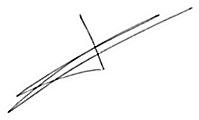
\includegraphics[width=120px,height=40px]{logo/signature200.png}\end{flushright} % signature

~\vfill
\begin{center}
	\begin{minipage}[c]{0.25\linewidth}
		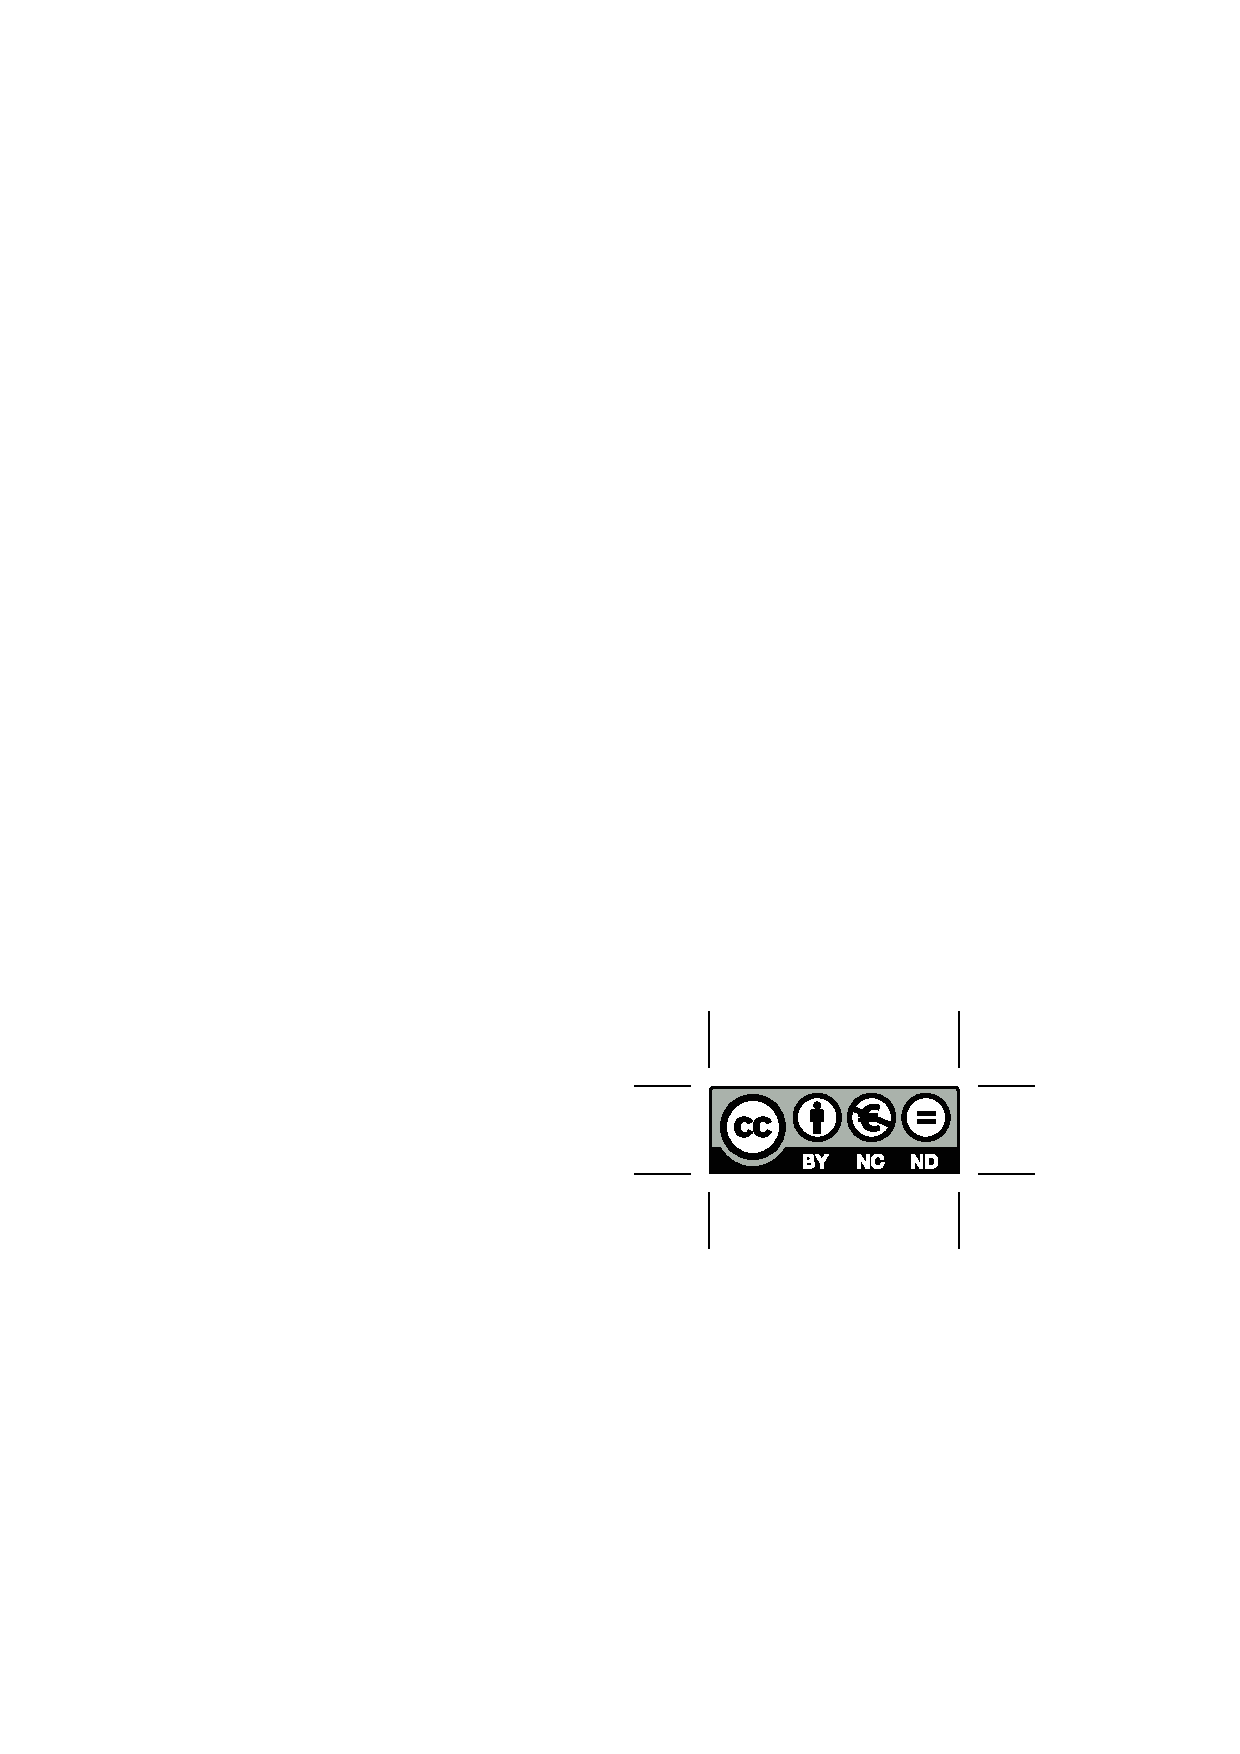
\includegraphics[height=35px]{logo/by-nc-nd-eu}
	\end{minipage}\hfill
\end{center}

Cette \oe{}uvre est mise à disposition selon les termes de la \href{https://creativecommons.org/licenses/by-nc-nd/4.0/deed.fr}{Licence Creative Commons Attribution - Pas d’Utilisation Commerciale - Pas de Modification 4.0 International}.


	\chapter*{Résumé}					%% résumé
    \addcontentsline{toc}{chapter}{Résumé}
	Cette thèse explore le rôle des changements dans les dynamiques intergénérationnelles en économie en se concentrant sur les résultats distributionnels. 
Le premier chapitre explore le déclin de la part du travail dans un contexte de changement de structure de la population avec l’apparence des cohortes de boomer en France et aux Etats-Unis. Je soutiens que la substitution du travail par le capital opérée par les firmes est une conséquence des changements dans les institutions du marché du travail qui sont déterminées de manière endogène par la structure d’âge de la population. 
Le second chapitre décrit comment la polarisation sur le marché du travail a été accompagnée par un déclin de la mobilité sociale intergénérationnelle au Royaume-Uni. Mes co-auteurs et moi comparons deux cohortes britanniques qui sont entrées sur le marché du travail à deux moments qui diffèrent considérablement en termes de structure d’emploi. Nous trouvons que le rôle du revenu parental a augmenté pour la mobilité sociale. Nous suggérons que la compréhension des dynamiques intergénérationnelles nécessite de comprendre la mobilité intragénérationnelle. 
Le troisième chapitre examine les conséquences des événements majeurs dans la vie sur les valeurs individuelles tout au long du cycle de vie. Je développe un cadre théorique pour expliquer comment les individus ajustent leurs valeurs quand elles sont interdépendantes et affectées par des chocs dus aux événements de la vie. En utilisant des données de cohortes britanniques, je montre que les expériences de la vie changent les valeurs des individus directement mais aussi indirectement puisque les individus cherchent à être cohérents dans leurs valeurs.

\vspace{0.5cm}
\noindent\textbf{Mots clés}: Dynamiques intergénérationnelles; Part du travail; Mobilité sociale; Valeurs individuelles\\
% \textbf{Classification JEL}:


	\chapter*{Abstract}					%% abstract
    \addcontentsline{toc}{chapter}{Abstract}
	This thesis explores the role of changing inter-generational dynamics in Economics with a focus on distributional outcomes. The first chapter explores the decline of the labor share in the context of the appearance of boomer cohorts in France and the US. I build a theoretical framework in which a generational conflict arises because young and old individuals have different income sources and opposite objectives in terms of public policy. I argue that the shift away from labor toward capital by firms is a consequence of changes in labor market institutions which are endogenously determined by the age structure of the population. The second chapter describes how polarization in the labor market has been accompanied by a decline in inter-generational social mobility in the UK. My co-authors and I compare two British cohorts that entered the labor market at two points in time that differed considerably in terms of the structure of employment. We find that the role of parental income has increased for social mobility. We suggest that understanding inter-generational dynamics requires considering how individuals move from their entry jobs into other employment categories, i.e. understanding intra-generational mobility. The third chapter examines the consequences of life-changing events on individuals’ values over the lifecycle. I develop a theoretical framework to explain how individuals adjust their values when those latter are inter-dependent and shocked by life events. Bringing the model to British cohort data, I show that life experiences change individuals’ values directly but also indirectly as spillover effects appear when individuals seek consistency in their values.

\vspace{0.5cm}
\noindent\textbf{Keywords}: Inter-generational dynamics; Labor share; Social mobility; Individuals' values\\
% \textbf{JEL classification}:

	\chapter*{Acknowledgements}			%% remerciements
    \addcontentsline{toc}{chapter}{Acknowledgements}
	First of all, I am grateful to Cecilia García Peñalosa and Marc Sangnier. I would like to thank them for their time and help all along this journey. I once summarized those three very diversified chapters to someone, and that person asked me: ``Who's the madman supervising this?''. I could never thank them enough for their intellectual flexibility in that respect. I have learned so much from them since they both decided to supervise my master's dissertation, then this thesis. I would like to thank them for being two brilliant professors and wonderful human beings.

I wish to thank the other members of my Ph.D. committee for their time and very accurate comments. 
Yanos Zylberberg invited me to the University of Bristol and provided me with incredibly useful advice and comments during those few months. I am grateful for his humor and enthusiasm which helped me to cope with this job market year. 
Xavier Raurich was my professor when I was in Erasmus at the Universitat de Barcelona. I am grateful for his interest and support since then. I am deeply convinced that his course motivated me to enroll in this Ph.D. journey while I was only a master's student. 
Giovanni Pica and Thierry Verdier are among the scholars that I enjoyed the most reading their papers. I am grateful to them as they helped improve the quality of my thesis through their comments.

I am grateful to the Aix-Marseille School of Economics as an institution and to all its members that I met during my time there. Karine Gente and Carine Nourry allowed me to do an internship as a research assistant when I was only in my third year. I am grateful to them for this opportunity which was also key in the decision to enroll in a Ph.D. years after. 
I am also grateful to all professors that I met and discussed with along those years, especially, Patricia Augier, Nicolas Berman, Renaud Bourlès, Bruno Decreuse, Eva Moreno-Galbis, Lorenzo Rotunno, Avner Seror, Tanguy van Ypersele, and Roberta Ziparo. 
I wish to thank the administrative team for their support and effectiveness, especially, Marine Boléa, Patrice Cacciuttolo, Anne-Sophie Leclercq Therond, Elisabeth Lhuillier, and Bernadette Vouriot.
I would like to express my gratitude to all former and current PhD students from AMSE with whom I shared very enjoyable moments, especially, Daniela Arlia, Stéphane Benveniste, Laurène Bocognagno, Kenza Elass, Jordan Loper, Nandeeta Neerunjun, Julieta Peveri, Morgan Raux, Laura Sénécal, Rosnel Sessinou, Mathilde Valéro, Sarah Vincent, and Rémi Vives.

My deepest thanks are addressed to both my family and my friends for their support all along those years, especially, 
Jade Benzaki, Tamara Casanova, Hugo Chirossel, Nicolas Court,
Ginette Galliano, Marc Galliano, Marie-Anne Galliano, Nicolas Galliano, Pierette Galliano,
Ombeline Jullien de Pommerol, Philippe Lavall, Fabien Martinet, Luke Mcgee O'Collins, Lucas Motta,
Jérôme Petit, Maryse Petit, Maxime Petit, 
Julie Pierson, Céline Prella, Jean-Marc Prella,
and Yohann Serot.
	
    \microtypesetup{protrusion=false}	%% désactive la protrusion (TOC LOFT GLS)
    	\tableofcontents				%% TOC
    	\listoffigures					%% LOF
    	\listoftables					%% LOT
    \microtypesetup{protrusion=true}	%% rétabli la protrusion

	\chapter*{General Introduction}
	\addcontentsline{toc}{chapter}{General Introduction}
    \markboth{General Introduction}{General Introduction}
	Each individual belongs to a generation that was preceded by other generations and will be followed by others. Studying the dynamics of socio-economic contexts between and within those generations is crucial to academic research to understand how individuals relate to their elders, their peers, and their youngsters. This thesis presents three academic contributions to the role of inter-generational dynamics in driving distributional outcomes in several strands of the literature such as macroeconomics, labor economics, and behavioral economics.

Each generation has gone through different timelines, events, and experiences. For instance, in Western Europe, the Silent Generation (1928-1945) has known World War II, the Baby Boomers (1946-1964) were raised during the 30-year post-war boom, Generation X (1965-1980) has grown up with the first generation of personal computers, while the Millennials (1981-1996) with the Web 2.0, lastly, the Zoomers (1997-2012) were either masked or online at school due to COVID-19.
Those differences can lead to diverging perceptions of the world, hence, preferences that themselves can generate inter-generational conflicts (\citealt{meisner2021you}). My first chapter entitled ``Inter-generational conflict and the declining labor share'' argues that conflicts between generations can have consequences for distributional outcomes.

In that chapter, I emphasize the role of demographic dynamics in the allocation between capital and labor when there are conflicts between generations to determine the public budget allocation. While the labor share remained stable for decades, several OECD countries have witnessed a decline since the beginning of the 1970s (\citealt{Elsby2013Decline}, \citealt{Karabarbounis2014Global}). A heated debate among economists has emerged trying to understand the reasons for these dynamics. Yet, the literature on the labor share has paid no attention to the coincidence in timing between, on the one hand, the start of the decline of the labor share, and on the other hand, the entry of the baby-boomer cohort into adulthood, i.e. entering into the labor market and reaching voting age. 
Thus, this chapter contributes to the growing literature on the demographic determinants of technological change and automation (\citealt{Acemoglu2018Race, Acemoglu2020Robots}). I argue that the observed shift away from labor toward capital is a response to changes in labor market institutions endogenously determined by the age structure of the population, a novel mechanism that this chapter is the first to identify. 

Entering the labor market is a crucial step for every individual. Among all the differences that generations face throughout their lifecycle, the difference in labor market context is likely to be one of the most diverging.\footnote{According to OECD data, a young boomer who entered in the US labor market in 1969---at the peak of the post-war economic boom---faced a 3.51\% unemployment rate, while a young millennial who looked for a job in 2009---during the Great Recession---faced a 9.27\% unemployment rate.}
Over the last decades, the labor market has been transformed due to institutional changes (\citealt{Bentolila1990Firing}, \citealt{Bentolila2003Explaining}) and technological change, notably, with the appearance of robots and automation technologies (\citealt{Acemoglu2020Robots}). Those latter have resulted in a rise in the share of low- and high-paying jobs at the cost of middling jobs, hence, polarizing the labor market (\citealt{Autor2003Skill}, \cite{Goos2007Lousy}). 
Meanwhile, inter-generational mobility has substantially declined in countries where the polarization process has been observed; see, for example, \citet{Blanden2007Accounting} for the UK and \citet{Chetty2020Race} for the US.
My second chapter entitled ``Spreading the polarization disease: From the labor market to social mobility'' suggests that increased employment polarization may be one of the factors behind the observed decline in inter-generational mobility.

In this chapter, written with Cecilia García-Peñalosa and Tanguy van Ypersele, we use data for two British cohorts that entered the labor market at two points in time that differed considerably in terms of the structure of employment to re-examine the drivers of mobility. The data indicate that occupational changes over the individual’s career are an important source of mobility, with large shares of those in low-paying (respectively, middling) occupations moving into middling (resp. high-paying) ones. When we compare the two cohorts we find that these two sources of mobility have declined for the younger cohort and that, whatever the initial occupation, parental income has become more important in leading to occupational upgrading. Moreover, we also document that the impact of parental income increased the most in the regions where the share of middling employment fell the most. We thus bridge a gap between two literatures, one focusing on falling mobility in high-income economies and another establishing an increase in job polarization in those same countries. This chapter adds to the previous one by suggesting that the relationship between technological change and generations is two-way. On the one hand, technological change can be due to institutional changes triggered by the age structure of the population (chapter one). On the other hand, individuals all along that structure do not experience the same type of inter-generational mobility as they face different labor market contexts owing to technological change.

Between and within generations, individuals experience different patterns of social and income mobility which tend to influence their preferences for redistribution (\citealt{Piketty1995Social}, \citealt{Alesina2018Intergenerational}). However, one can think of many life experiences that can affect other types of preferences (e.g. for leisure or for fertility). Values characterize preferences as they reflect what is important in individuals' lives. Studying the dynamics of the former is key to understanding differences in preferences between economic agents which can explain differences in behavior, hence, gaps in economic outcomes. While prior work analyzes those dynamics, it only focuses on the evolution of a single value, thus, neglecting that values are inter-dependent across groups.\footnote{See, for example, \citet{Bolzendahl2004Feminist}, \citet{Cunningham2005Reciprocal}, \citet{Fernandez2007Women}, \citet{Washington2008Female}, and \citet{Grinza2017Entry}.} My third chapter entitled ``Spillover effects across values'' shows that assuming independence between values leads to underestimating to which extent life experiences affect individuals because such an assumption omits the consequences of the group membership, hence, the existence of spillover effects.

In this chapter, I argue that because group identity is defined by a cluster of values, shocks to one value that induce a change in group membership will lead to changes in other values, hence creating spillover effects. 
Those spillover effects appear when individuals seek to be consistent with the values of the group with which they identify. To elucidate the spillover effects, I build a theoretical model accounting for values consistency and endogenous group membership. Using British cohort data, I identify spillover effects through the impact of exogenous life events on values (conservatism and collectivism) in a simultaneous equations model. I also show that changes in values following life events are also associated with a change in the likelihood to vote for different political parties. My results show that individuals adjust the full set of their values when an experience occurs in their life. The findings suggest that value consistency and group identity are key drivers of values dynamics, hence, preferences. Thus, this chapter contributes to the literature on the formation of preferences in which most prior work focuses either on the inter-generational transmission (\citealt{Bisin2001Economics, Bisin2011Economics}) or the development during childhood (\citealt{Fehr2013Development}, \citealt{Doepke2017Parenting}). I, instead, provide a new mechanism---which takes place later on in individuals' lifecycle---that is based on the will to convey values that are consistent with the group with which individuals belong, hence identify. This chapter also suggests that the link between cultural values and institutions, as described by \citet{Acemoglu2021Culture}, may find its origins in the willingness of individuals to group and share consistent values.

This thesis contributes to several strands of the literature in economics (including macroeconomics, labor economics, and behavioral economics) by adopting an inter-disciplinary approach as I build on psychology and sociology, hence, bridging key literatures in social sciences. The central theme of this thesis relates to the existence of several generations embodied with individuals that are different between and within those generations due to their individuals' experiences over the lifecycle which in turn have consequences for institutions, values, and economic outcomes.

\printbibliography[heading=subbibliography]
    \clearpage
	\ohead{\leftmark\ifstr{\rightmark}{\leftmark}{}{ -- \rightmark}} %% place le chapître et la partie en en-tête

	\chapter{Inter-generational conflict and the declining labor share}\label{chap1}
	\noindent \textbf{Abstract}: The coincidence in timing between the start of the decline of the labor share and the entry of the baby-boomers cohort into adulthood---entering the labor market and reaching voting age---has received no attention. I argue that the observed shift away from labor toward capital is a response to changes in labor market institutions endogenously determined by the age structure of the population through voting. The size of the boomer cohort gives them large political weight and allows them to change public policy in their favor when they are young and then old. These institutional changes have consequences for the wage bargaining to which firms respond by substituting labor with capital to thwart workers’ appropriation of the rents. I develop a model which links public policy to wage bargaining and calibrate it for France and the US. Numerical simulations can replicate the decline of the labor share and labor market dynamics.\\
\vspace{1em}\\
\noindent\textbf{Keywords:} Labor share, Inter-generational conflict, Wage bargaining, Probabilistic voting.\\
\noindent\textbf{JEL Codes:} E25, J11, J52.

\clearpage
\chaptertoc{}

\pagebreak

\begin{refsection}

    %%% CONTENT OF THE CHAPTER
    
    \section{Introduction} \label{chap1-introduction}
    % Motivation
The labor income share, its evolution and distributional implications, have been of interest for economists since at least the work of \citet{Kaldor1955Alternative}.\footnote{Starting with \citet{Blanchard1997Medium} a growing literature has documented changes in the labor share. A renewed interest in its distributional consequences is largely due to \citet{Atkinson2009Factor}, and it is a key determinant of the distribution of personal income; see \citet{Checchi2010Labour} and \citet{Bengtsson2018Capital}.}
While initially existing evidence indicated that it remained stable for decades, several OECD countries have witnessed a decline since the beginning of the 1970s and a heated debate has emerged trying to understand the reasons for these dynamics; see, for example, \citet{Karabarbounis2014Global} and \citet{Elsby2013Decline}. These countries also experienced significant changes in the age structure of their population following the birth of the so-called \textit{baby-boomer} cohorts---born between 1945 and 1965. 
Yet, the literature on the labor share has paid no attention to the coincidence in timing between, on the one hand, the start of the decline of the labor share, and on the other hand, the entry of this latter cohort into adulthood, i.e. entering into the labor market and reaching voting age.

% Empirical motivation
Figure \ref{chap1-fig:emp-lsdepcor} depicts the negative correlation between the old-age-dependency ratio---which is driven by the position in the life cycle of the boomer cohorts---and the labor share across several OECD countries between 1950 and 2019.\footnote{The old-age-dependency ratio is defined as the ratio of the number of individuals above 60 over the number of those between 20 and 60. When the boomers are young, they maintain the old-age-dependency ratio relatively low although their elders are aging due to the increasing life expectancy. Once they become old, the ratio explodes.}
% Empirical motivation
\begin{figure}[!tb]
	\centering
	\caption{Labor share and old-age-dependency ratio}\label{chap1-fig:emp-lsdepcor}
	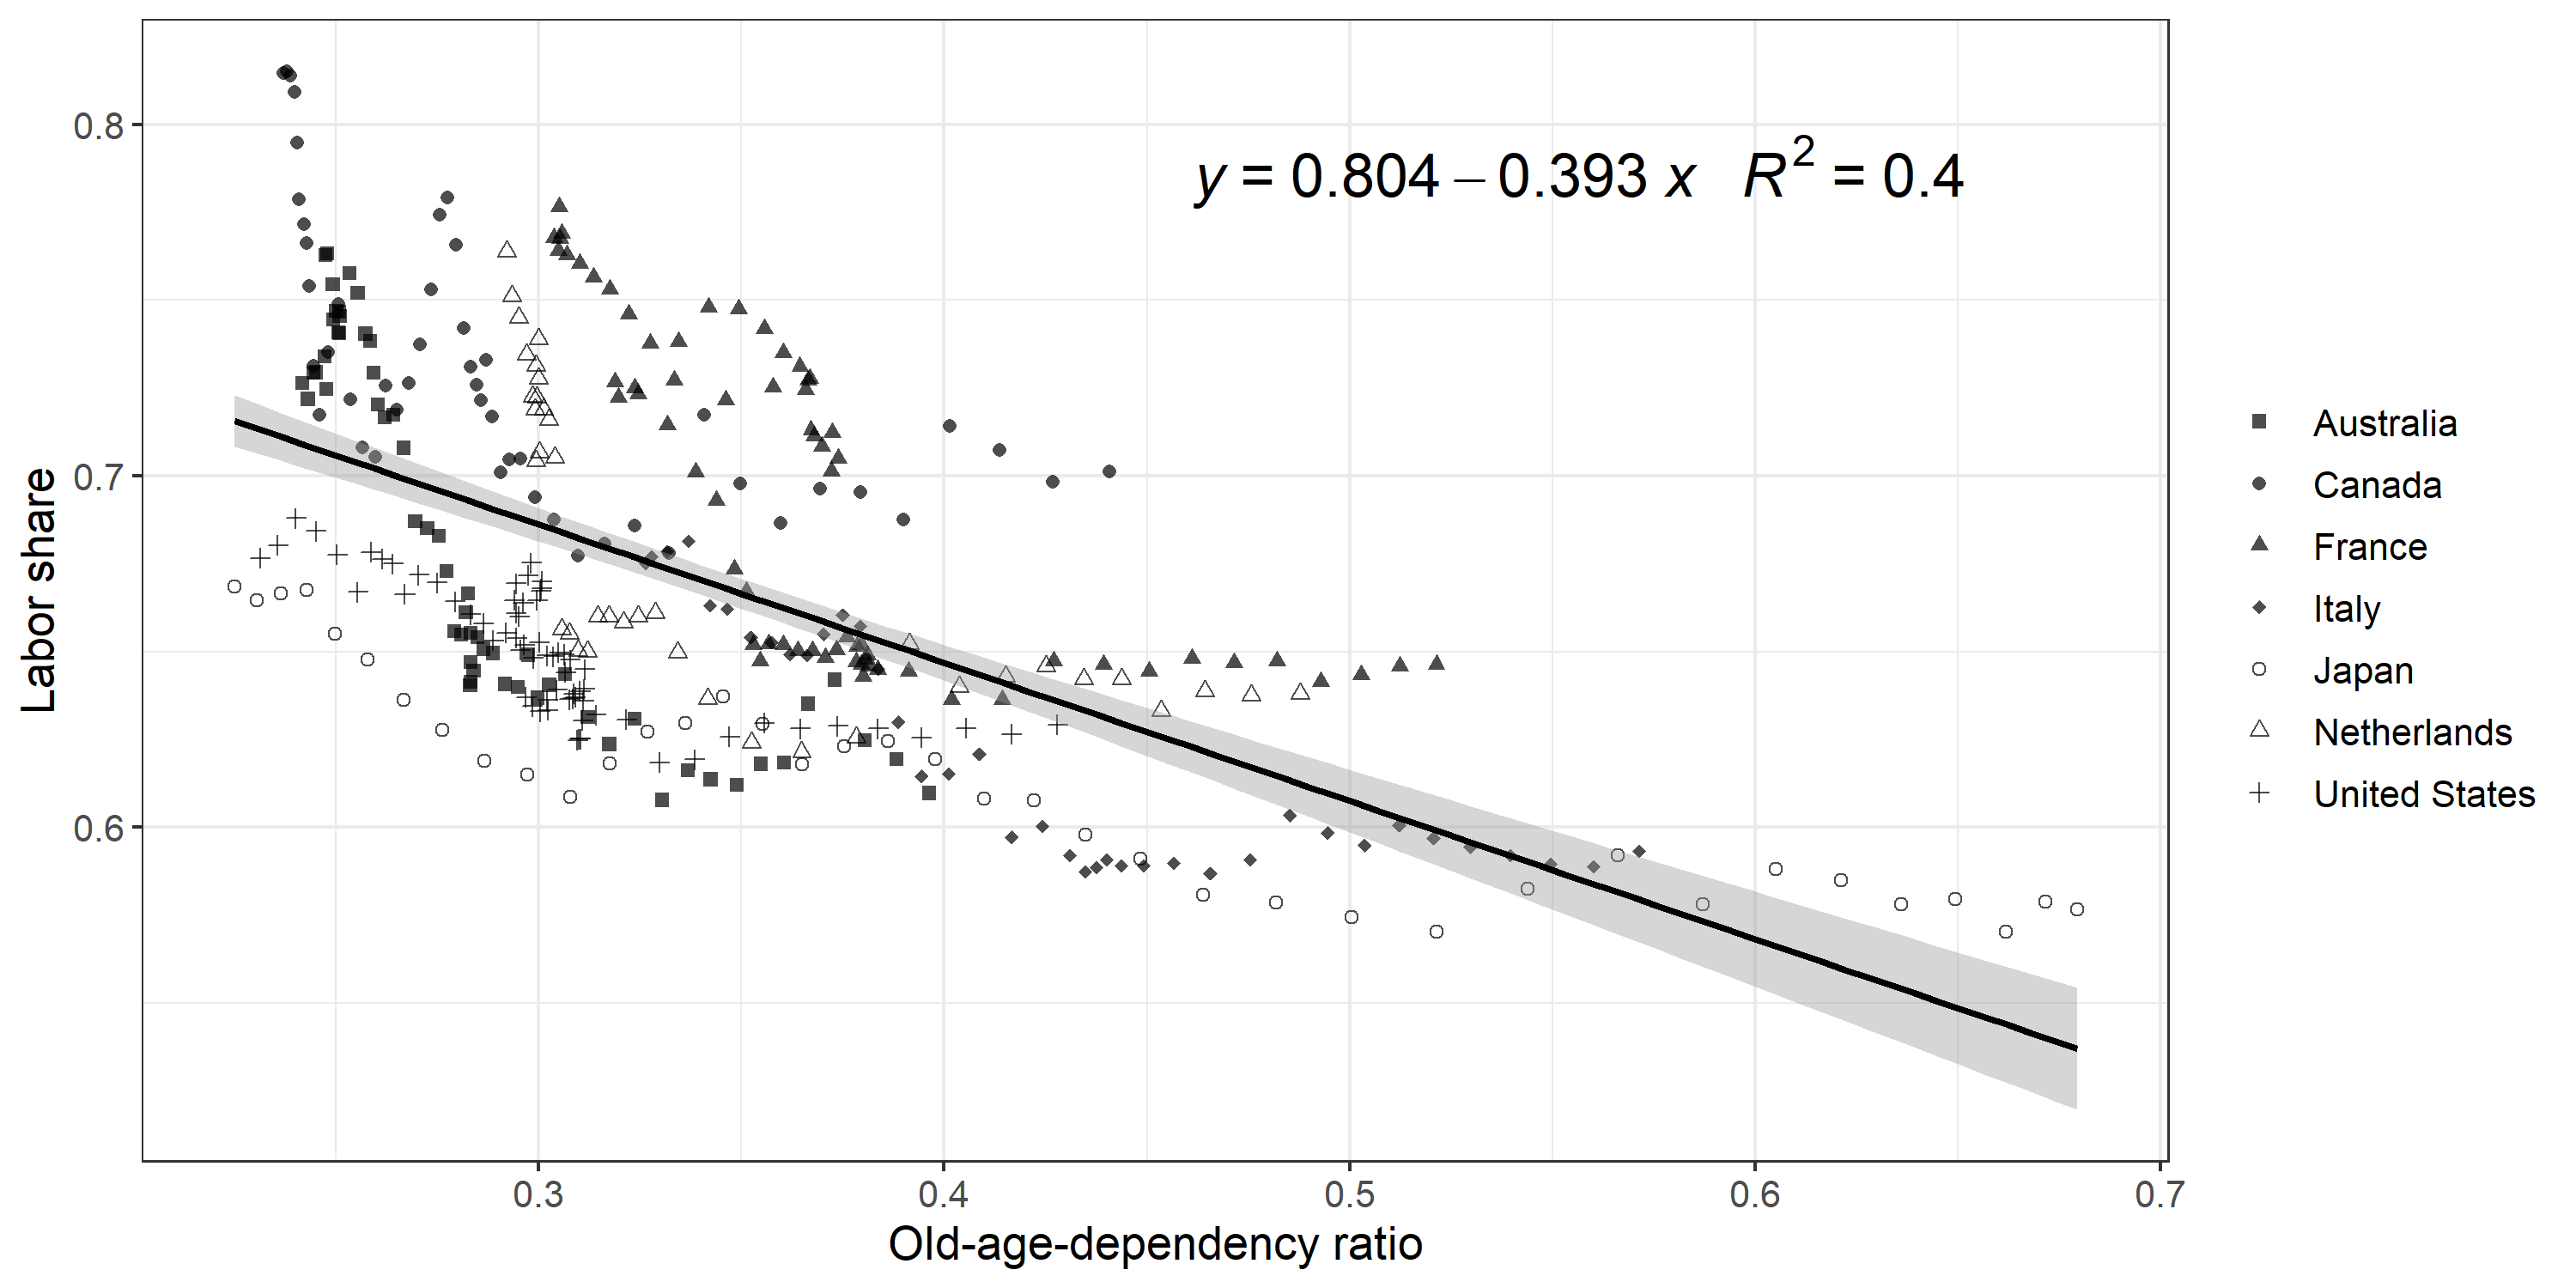
\includegraphics[width=\linewidth]{chap1/graphic/emp-lsdepcor.png}
	\vspace{-3em}
	\justify\singlespacing\footnotesize\textit{Notes:} The figure displays the negative correlation between the labor share and old-age-dependency ratio for several OECD countries. Labor share data are from the \href{https://www.rug.nl/ggdc/productivity/pwt/}{Penn World Table 10.0}. The old-age-dependency ratio is defined as the number of individuals above 60 over the number of those between 20 and 60. The ratio is computed with demographic data from the ``medium variant'' estimates from the \href{https://population.un.org/wpp/}{United Nations World Population Prospects 2017}.
\end{figure}
These data display a positive correlation, as the older the population the lower the labor share. 
Figure \ref{chap1-fig:emp-pubdepcor} shows cross-country correlations between the old-age-dependency ratio and the ratio between two public policy instruments, thus, providing empirical motivation also for linking public policy to the age structure of the population.\footnote{Looking also at the timing of labor market reforms---on employment protection legislation, public pension systems, non-employment benefits, and migration policies---in 14 OECD countries between 1986 and 2005, \citet{Pica2010Capital} shows that the number of reforms raising labor market flexibility has increased over time, hence, as the boomers' cohorts aged.}
\begin{figure}[!tb]
	\centering
	\caption{Public pension to unemployment spending ratio and old-age-dependency ratio}\label{chap1-fig:emp-pubdepcor}
	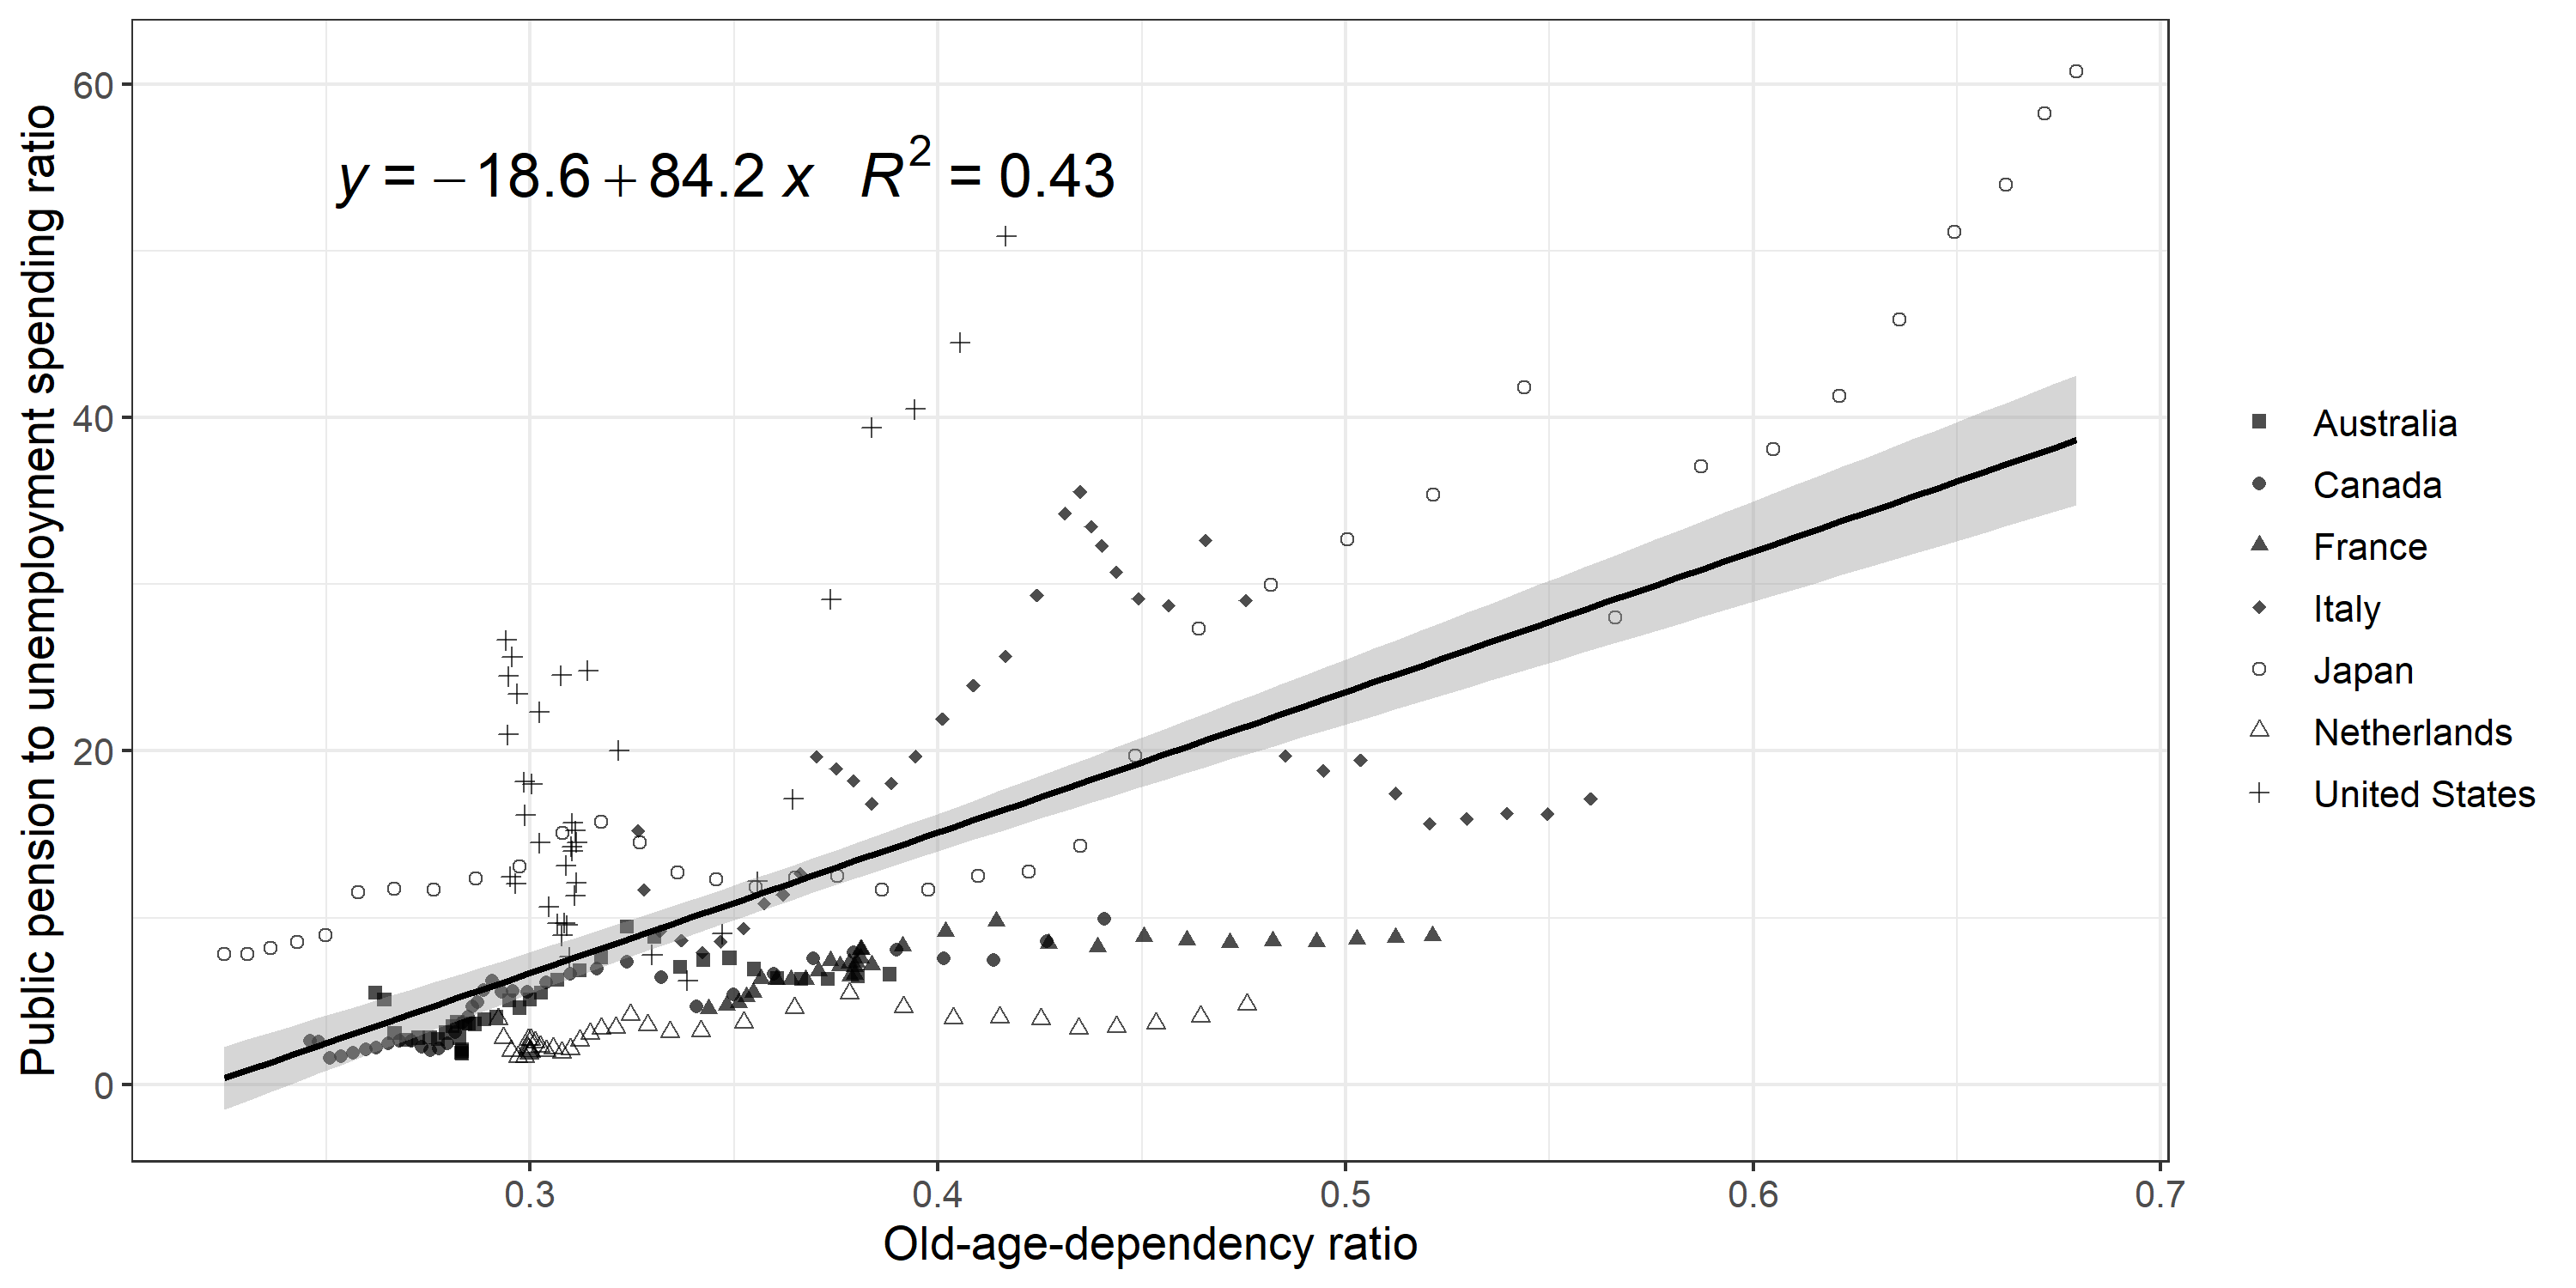
\includegraphics[width=\linewidth]{chap1/graphic/emp-pubdepcor.png}
	\vspace{-3em}
	\justify\singlespacing\footnotesize\textit{Notes:} The figure displays the positive correlation between the public pension to unemployment spending ratio and old-age-dependency ratio for several OECD countries. The public pension to unemployment spending ratio is computed using the total public unemployment spending and the total public pension spending (both as shares of GDP) from the OECD data. The old-age-dependency ratio is defined as the number of individuals above 60 over the number of those between 20 and 60. The ratio is computed with demographic data from the ``medium variant'' estimates from the \href{https://population.un.org/wpp/}{United Nations World Population Prospects 2017}.
\end{figure}
An increase in the old-age dependency ratio is associated with an increase in public pensions as a share of GDP relative to the share of unemployment spending. These data indicate that as the boomer cohorts age, public policy shifts in favor of old-age specific government spending.

% In this paper
In this paper, I argue that the observed shift away from labor toward capital is a response to changes in labor market institutions endogenously determined by the age structure of the population, a novel mechanism that this paper is the first to identify. Through this new \textit{policy-mechanism} effect, boomers drove the decline of the labor share when they were young and continue to drive it down nowadays as they retire. 

My argument is based on the idea that the boomers drive public policy choices because the size of their cohort gives them large political weight. When they are young, they change labor market institutions in their favor which allows them to bargain greater wages. To thwart workers' appropriation of rents, firms shift away from labor toward capital which decreases the labor share. Once the boomers become old and retire, we would expect a reversal of the labor share dynamics as pro-worker labor market institutions dwindle which increases employment. However, the consequent positive effect of employment on the labor share is offset by the capital accumulation fostered by extensive savings of the boomers when they were young, implying a further decline.

%% What I do
% Describe model
I develop a two-period OLG model with young and old households. Both vote to determine public policy while they have different income sources and opposite objectives. Old agents receive capital income and favor old-age specific government spending, whereas the youth receive wages and support unemployment benefits as they face unemployment risk. As a large cohort of boomers arrives, they use their political weight---through voting---to raise taxes and unemployment benefits. Both latter increase the outside option of workers in wage bargaining which allows them to bargain greater wages. The representative firm shifts away from labor toward capital. When labor and capital are gross substitutes, this leads to the decline of the labor share. Once the boomers retire, the political weight of the young declines and so does the unemployment benefit which fosters employment. However, the positive effect of employment on the labor share is offset by capital accumulation due to the extensive savings of young boomers which have been fostered by their higher bargained wages.

% Two mechanism
My framework suggests that demographic dynamics affect the labor share in two different ways. On the one hand, there is a direct \textit{factor-accumulation} effect operating through the labor supply and capital stock. A large generation expecting to live longer, such as the boomers, results in a higher labor supply when they are young and a larger capital stock---fostered by their savings---once they retire. On the other hand, there is an indirect \textit{policy-mechanism} effect reflecting the inter-generational conflict over public policy. A large generation has relatively more political weight---with respect to their elders and their youngsters---which allows it to shape the public budget allocation in its favor through voting.

% Consequences on the labor market
Both effects have consequences for the wage bargaining taking place in the labor market. The factor-accumulation effect encompasses two dynamics: a larger capital stock allows firms to substitute labor with capital which increases the capital-to-labor ratio; while a greater labor supply decreases wages which fosters employment, hence reducing the capital-to-labor ratio. Conversely, the consequence of the policy-mechanism effect is straightforward. When the political weight of the youth increases, so do unemployment benefits which raise workers' outside option. Workers bargain greater wages which undermines employment as firms substitute labor with capital, hence, raising the capital-to-labor ratio. The framework provides dynamics of the capital-per-worker with respect to demographic dynamics that \textit{do not depend on} the elasticity of substitution between capital and labor.

% Elasticity of substitution
The elasticity of substitution between capital and labor plays a crucial role in the model as it determines whether an increase in capital per worker raises or reduces the labor share. To calibrate the model, I estimate this elasticity, respectively, for France and the United States, and find, respectively, the values 1.21 and 1.27.\footnote{
I follow the specification of \citet{Klump2007Factor}, I estimate a single-equation estimation from the two first-order conditions of the profit maximization for a CES production function with biased technical change. Periods of the estimate correspond to 1950-2018 for France and 1950-2019 for the US. See section \ref{chap1-calibration} for the details.} 
Both elasticities being greater than one imply that capital and labor are gross substitutes. Thus, any increase of the capital per worker decreases the labor share, which corresponds to the stylized facts for several OECD countries (\citealt{Karabarbounis2014Global}). There is a substantive debate about the value of this elasticity in the literature. For the United States, many studies tend to find an elasticity between 0.4 and 0.6 (\citealt{Antras2004Aggregate}, \citealt{Chirinko2008Sigma}, \citealt{LeonLedesma2010Identifying}, i.a.). Nonetheless, \citet{Chirinko2017Substitution} recently show that this elasticity is much greater than one when considering income shares defined net of depreciation, which is in line with my theoretical framework. \citet{Rognlie2016Deciphering} also argues that accounting for depreciation is more relevant when dealing with income distribution issues. My estimate builds on the two latter arguments and supports recent estimates considered in the labor share literature.\footnote{
\citet{Caballero1998Jobless} use a capital-labor elasticity of substitution about 6 to simulate French data. \citet{Karabarbounis2014Global} use cross-sectional data on 50 countries between 1975 and 2012 to find a baseline estimate of the elasticity about 1.28. \citet{Piketty2015About} shows that the capital-income ratio and capital share tend to be positively correlated, thus, arguing that only an elasticity above one can reconcile this stylized fact with the one-sector standard model.}

% Quantitative analysis
I calibrate the model for France and the US starting in 1950. The model replicates labor share dynamics until the 2010s, along with those of the labor market. It also provides predictions of future dynamics. In France, the labor share is predicted to steadily decline from 64.7\% in 2020 to 60.4\% by 2100; while in the US, it is predicted to remain stable at 62.7\% until 2040 before declining to 58.8\% by 2100. From 2020 onward and until the end of the century, on average, about one percentage point of the labor income share will shift to capital income every 20 years.

% Counterfactual and decomposition
Counterfactual analysis shows that the policy-mechanism effect is as important as the factor-accumulation effect. In fact, the former partially offsets the latter effect when the boomers are young, hence, reducing the labor share. Once they retire, this newly-identified effect dominates. This pattern holds for both countries.

% Who are the winners
Lastly, I conclude by showing that boomers are the winners of the age-related conflict despite the decline of the labor share when they are young. They manage to compensate their labor income losses through redistribution due to their political weight. Thus, boomer cohorts have been better off in terms of income with respect to their elders and their youngsters.

%% Contributions
% 1/ Consequences of changes in the age structure of the population
My paper is related to several strands of the literature. First, I contribute to the growing literature on the consequences of demographic changes for the allocation between capital and labor income. 
\citet{Schmidt2013Demographic} show that an aging population leads to more savings, hence, more capital. When capital and labor are gross
substitutes, the accumulation of capital shrinks the labor share. 
I build on their mechanism--- which I define as the direct factor-accumulation effect---and introduce a new mechanism, namely, the indirect policy-mechanism effect. %, suggesting that labor market institutions are endogenous to these population dynamics.
\citet{Albis2021Demographic} empirically find that an exogenous change in the net population growth rate leads to a decline of the labor share; while an exogenous change in the net migration rate increases the labor share.
My paper provides a theoretical framework that can explain both patterns through the lens of the factor-accumulation and policy-mechanism effects.
Recent work has focused on changes in the labor share across industries. Notably, \citet{Acemoglu2022Demographics} argue that firms decide to rely more on automation technologies to replace middle-aged workers in manual production tasks as the latter become scarce due to population aging. They predict that the labor share should decline in industries that are intensive in those tasks.
My work provides an additional mechanism that relates firms' response to constraints in optimizing production factors owing to endogenous changes in labor market institutions fostered by demographic dynamics.

% 2/ Labor share determinants
Second, my work is related to the literature on the determinants of the labor share. These determinants have been widely studied and debated, ranging from globalization (\citealt{Jayadev2007Capital}, \citealt{Pica2010Capital}, \citealt{Young2018Globalization}, \citealt{Autor2020Fall}, i.a.) to capital-biased technical change (\citealt{Acemoglu2002Directed},  \citealt{Acemoglu2003Labor}, \citealt{Karabarbounis2014Global}, i.a.) and labor market institutions (\citealt{Blanchard1997Medium}, \citealt{Bentolila2003Explaining}, \citealt{Bental2010Declining}, i.a.). \citet{Caballero1998Jobless} argue that pro-labor income institutions are a burden to firms because they limit their ability to optimize inputs but also because they enable workers to obtain a high income share. As a response, firms shift away from labor toward capital through biased technical change. My paper looks upstream of the key mechanism in \citet{Caballero1998Jobless} and reproduces it without the need for biased technical change; rather I endogenize changes in labor market institutions which are determined by the age structure of the population. I hence show that demography is a key determinant of the labor share and suggest that it can be at the root of several explanations that the literature has measured (see, for instance, \citealt{Bergholt2021Decline}).

% 3/ Role of demography in shaping institutions and macro consequences
Third, the paper fits into the literature on the role of demography in shaping institutions and its consequences for macroeconomic outcomes (\citealt{Lee2010Macroeconomic}, \citealt{Aksoy2019Demographic}). Prior work focuses on the optimal retirement age for economic growth (\citealt{Futagami2001Population}, \citealt{Gonzalez-Eiras2012Ageing}, i.a.) or the sustainability of pension systems (\citealt{DelaCroix2013Aging}, \citealt{Dedry2017Aging}, i.a.). I contribute to this literature by providing insights on a key macroeconomic indicator that has never been considered by this debate, namely, the allocation of income between capital and labor.

% 4/ Boomers
Lastly, I contribute to the scarce literature on the consequences of cohort dynamics for aggregate labor-market dynamics (\citealt{Shimer1998Why}, \citealt{Ferraro2020Aging}). My results suggest that the boomers' generations are important drivers of the declining labor share in France and the US, a concept that has so far not been put forward.

% Plan
This paper is organized as follows. Section \ref{chap1-theory} describes the model starting with households, then presenting the labor market and public policy, to analyze the equilibrium. Section \ref{chap1-quantitative} provides the quantitative analysis. I start with the data, before calibrating the model. I present model predictions, compare the factor-accumulation and policy-mechanism effects, and discuss who are the winners of the age-related conflict. Section \ref{chap1-conclusion} concludes.
    
    \section{The model} \label{chap1-theory}
    %% Introduction of the model
% Household
I consider a two-period OLG model in which there are two types of households: young and old.
% Inter-generational conflict
The inter-generational conflict arises because young and old households have different preferences in terms of public policy; the former are in favor of higher unemployment benefits while the latter prefer more old-age specific government spending.

%%% Argue your choices (1 paragraph)
I model the inter-generational conflict over the public budget allocation with this trade-off between unemployment benefits and old-age specific government spending for two reasons.
%% 1/ Health expenditure are also for the young?
First, we can think about several types of government spending that are specific to old households. For instance, this can be interpreted as an old-age specific health expenditure or more broadly, public services such as residential care homes from which the elderly directly derive utility.\footnote{Although health spending is also for the young, it is correlated to age. \citet{Papanicolas2020Comparison} show that the US average per-capita health expenditure in 2015 is about three times larger for individuals above 65 with respect to those between 20 and 64. They also find an average ratio of about 3.14 for a sample of 8 OECD countries (excluding the US).}
%% 2/ Why don't you use a pension system?
Second, replacing this government spending with pensions would also be an alternative specification. Nonetheless, it would reduce the tractability of the model without any substantial gain in the analysis.\footnote{Pensions would introduce the policy instrument within the budget constraint of the old rather than directly in the utility function. From the point of view of the \textit{indirect policy mechanism}, the elderly would still desire more of this instrument. On the side of the \textit{direct factor-accumulation mechanism}, \citet{Schmidt2013Demographic} reach the same conclusions about the direct effect of aging on the labor share by considering an exogenous pension system. Moreover, additional assumptions would be required about the type of pension system, i.e. pay-as-you-go vs fully-funded pension system.}
To summarize, the model can be extended to other policy instruments for the old as long as they derive utility from it, either directly or through their income. The central point is to oppose young and old agents with different returns to policy instruments in utility terms.

Decisions within each period unfold as follows. First, young and old households vote to choose the tax rate, the unemployment benefit, and the old-age specific government spending, which defines the public policy equilibrium. 
Second, young households bargain over wages with the representative firm which determines the labor market equilibrium. 
Third, the uncertainty about the employment status of young households is resolved. 
Fourth, households choose their consumption and savings.
The vote and the bargaining jointly determine the equilibrium of the economy and, therefore, the labor share. I describe the model backward: starting with households, before presenting production and the labor market, and ending with the voting on public policy. Lastly, I analyze the equilibrium.

\subsection{Households}\label{chap1-households}

%% Demographic dynamics
The population consists of $N^y_t$ young and $N^o_t$ old individuals. Demographic dynamics are given by $N^y_t = n_t N^y_{t-1}$ where $n_t > 0$ is the gross rate of population growth, and $N^o_t = p_t N^y_{t-1}$ with $p_t \in \left(0,1\right]$ being the survival rate. The survival rate $p_t$ is an increasing function of life expectancy and a decreasing function of the retirement age.\footnote{In the model, agents are considered as old once they retire. If the life expectancy and the retirement age grow at the same rate, then the survival rate remains constant. For more details on the measurement of population aging, see \citet{Sanderson2007Perspective}; \citet{Sanderson2013Characteristics}; \citet{DAlbis2013Age}.} Both demographic parameters are exogenous and may vary over time. Their variations will generate population dynamics, and affect the old-age dependency ratio, $N^o_t/N^y_t = p_t/n_t$. 

%% Timing of the model and maximization program
Each cohort consists of a continuum of agents with identical preferences. Households have logarithmic utility functions and derive utility from consumption. Young households discount the future at factor $\alpha \in \left(0,1\right)$. They face an idiosyncratic longevity risk: with probability $p_{t+1}$ they survive and become old households in period $t+1$. Due to risk of death, the effective discount factor of young households equals $\alpha p_{t+1}$. 
Young households earn a disposable income $y_t$ that they allocate between consumption $c_{1,t}$ and savings $s_t$. 
Once old, they receive the net return of their savings $(1-\tau_{t+1}) s_t \hat{R}_{t+1}$, where $\tau_{t+1}$ is the tax rate and $\hat{R}_{t+1}$ the gross return on savings of a young household that survives to old age. I suppose a perfect annuities market where savings of young agents who die before becoming old are distributed among their surviving peers. Due to the perfect annuities market $\hat{R}_t = R_t/p_t$ where $R_t$ is the gross return on physical capital. Old households allocate all their capital income to consumption $c_{2,t+1}$ and also derive utility from old-age specific government spending $g_{t+1}$ which is a public good financed through taxes. This good can be interpreted as a variety of public expenditures---ranging from public provision of leisure activities to the pension of domestic helps---that increase the quality of life. Lastly, old households die at the end of period $t+1$.

% Maximization program
Maximizing expected utility, a household in period $t$ solves the following maximization problem:
\begin{align*}
	\max_{c_{1,t},~c_{2,t+1}}& U_t = \ln c_{1,t} + \alpha p_{t+1}\left( \ln c_{2,t+1} + \beta \ln g_{t+1} \right)\\
	\text{s.t.} ~~ &c_{1,t} + s_t = y_t,\\
	&c_{2,t+1} = (1-\tau_{t+1}) s_t \hat{R}_{t+1},
\end{align*}
% Define beta
where $\beta>0$ characterizes the preference for old-age specific government expenditure. The first-period disposable income $y_t$ depends on the employment situation of the household. Each young household faces an idiosyncratic unemployment risk with probability $u_t \in \left[0,1\right)$. The employment situation is known when choosing consumption and savings. An employed household earns a net wage $y_t^e= (1-\tau_t)w_t$ where $w_t$ is the wage rate, while an unemployed one gets the unemployment benefit $ y_t^u = b_t$ where $b_t$ are the unemployment benefits.

% FOC
Solving the household's maximization problem leads to the optimal consumption in both periods and savings in first period, which are
\begin{align}
	c_{1,t} &= \frac{1}{1+\alpha p_{t+1}} y_{t}, \label{chap1-eq:hhmaxc1}\\
	c_{2,t+1} &= \frac{\alpha p_{t+1}}{1+\alpha p_{t+1}}(1-\tau_{t+1})\hat{R}_{t+1}y_{t}, \label{chap1-eq:hhmaxc2}\\
	s_t &= \frac{\alpha p_{t+1}}{1+\alpha p_{t+1}} y_t. \label{chap1-eq:hhmaxs}
\end{align}
Since the utility function is logarithmic, savings are a constant proportion of disposable income. Aggregate savings in the economy are the weighted average of all disposable incomes of the young such that
\begin{equation}\label{chap1-eq:agg-saving}
	S_t = \frac{\alpha p_{t+1}}{1+\alpha p_{t+1}}\Big[(1-u_t)(1-\tau_t)w_t + u_t b_t\Big] N_t^y.
\end{equation}
I assume that capital fully depreciates between the two periods.\footnote{A period corresponds to half the lifetime of a generation, hence, I assume that capital is either depreciated or obsolete after such a long period.} Thus, equation \eqref{chap1-eq:agg-saving} determines the capital stock next period so that $K_{t+1} = S_t$. This assumption also implies that the gross return on physical capital is equal to the rental rate, i.e. $R_t = r_t$. 

\subsection{Labor market}\label{chap1-labor-market}

Consider a representative firm with a standard CES production function given by
\begin{equation}\label{chap1-eq:prod}
	Y_t = A\left[ \phi K_t^{\frac{\sigma - 1}{\sigma}} + (1-\phi) L_t^{\frac{\sigma - 1}{\sigma}}\right]^{\frac{\sigma}{\sigma-1}},
\end{equation}
where $K_t$ is the capital stock, $L_t$ labor, $\sigma$ the elasticity of substitution between capital and labor, $\phi$ the factor share parameter capturing the relative importance of inputs in production and $A$ a scale parameter. 
Rewriting the production function in per-worker terms, I have
\begin{equation}\label{chap1-eq:prod/L}
	\frac{Y_t}{L_t} = A\left(\phi k_t^{\frac{\sigma-1}{\sigma}} + 1-\phi\right)^{\frac{\sigma}{\sigma-1}},
\end{equation}
% Define k_t
where $k_t\equiv K_t/L_t$ is capital-per-worker.
The inverse labor demand function obtained from profit maximization is
\begin{equation}\label{chap1-eq:labor-demand}
	w_t = (1-\phi)A\left(\phi k_t^{\frac{\sigma-1}{\sigma}}+1-\phi\right)^{\frac{1}{\sigma-1}}.
\end{equation}

% Define labor share
% As long as the representative firm is on its labor demand curve, t
The labor share is defined as the ratio between the wage rate and output-per-worker, i.e. $\theta_t \equiv w_tL_t/Y_t$.
%
Using equations \eqref{chap1-eq:prod/L} and \eqref{chap1-eq:labor-demand}, the labor share is given by
\begin{equation}\label{chap1-eq:theta}
	\theta_t = \left(1+\frac{\phi}{1-\phi}k_t^{\frac{\sigma-1}{\sigma}}\right)^{-1}.
\end{equation}
%
Note that when the capital-labor elasticity of substitution equals unity, then the labor share is constant, i.e. $\theta_t=1-\phi$.
%
From equation \eqref{chap1-eq:theta}, we can also define the labor-to-capital income ratio as
\begin{equation}\label{chap1-eq:Theta}
	\Theta_t \equiv \frac{\theta_t}{1-\theta_t} = \frac{1-\phi}{\phi}k_t^{\frac{1-\sigma}{\sigma}}.
\end{equation}

The comparative statics of these expressions are straightforward. A higher capital-per-worker increases the wage and output per worker, i.e. $\partial w_t/\partial k_t > 0$ and $\partial (Y_t/L_t)/\partial k_t > 0$. However, the impact on the labor share depends on the elasticity of substitution between both factors, with $\partial \theta_t/\partial k_t \lessgtr 0$ if $\sigma \gtrless 1$. To have a negative relationship between the capital-per-worker and the labor share, both factors have to be gross substitutes, i.e. $\sigma > 1$. In such a case, any increase in capital per worker leads to a higher wage that is outweighed by the increase in output per worker. Thus, the labor share declines along with the labor-to-capital income ratio.

Young households bargain over the wage rate with the representative firm. The employer retains the prerogative to hire and fire as the labor market is a monopsony.\footnote{Possible extensions of the model would be to consider either a ``right-to-manage'' model \textit{à la} \citet{Nickell1983Unions} or an ``efficient contract'' model \textit{à la} \citet{McDonald1981Wage}. Both specifications introduce a representative union to bargain with the representative firm which strengthens the relative bargaining power of the workers by adding a distortion to the wage. In those settings, the bargaining power can be endogenous to public policy. Nonetheless, this goes far beyond the scope of the paper. With exogenous bargaining power, the right-to-manage specification leads to qualitatively equivalent results.} Consequently, the firm is always on its labor demand curve and equation \eqref{chap1-eq:labor-demand} holds. Since workers compete to get employed, they subsequently undercut their wages so that the wage rate is pinned down to their incentive constraint. The incentive constraint of workers is such that the net wage cannot be lower than their outside option, namely, the unemployment benefits, i.e. $(1-\tau_t)w_t \geq b_t$. Therefore, the labor market equilibrium wage---which implicitly characterizes the level of employment $L_t$---becomes
\begin{equation}\label{chap1-eq:labor-market}
    w_t = \frac{b_t}{1-\tau_t}.
\end{equation}

Using the labor demand function, as given by equation \eqref{chap1-eq:labor-demand}, I obtain $dL_t/db_t<0$ and $dL_t/d\tau_t<0, \forall \sigma$. When the unemployment benefit or the tax rate increase, so does the workers' outside option. As a result, workers bargain greater wages and the firm shifts away from labor toward capital to thwart workers' appropriation of the rents, i.e. the increase of labor costs. Therefore the model is able to replicate the partial equilibrium effect in \citet{Caballero1998Jobless} \textit{regardless of} the value of the elasticity of substitution between labor and capital.

\subsection{Public policy}\label{chap1-public-policy}

%% Describe government in the model (1 paragraph)
% Government revenue
The government taxes the labor income of the young and the returns to savings of the old at the same tax rate.\footnote{I consider a common tax rate to simplify the analysis. Young and old agents, both prefer a lower tax rate as it reduces their disposable income. By introducing different labor and capital income tax rates, I would have two sources of inter-generational conflict, adding complexity to the voting process but without providing additional insights.} The revenue generated from these taxes is allocated to unemployment benefits and old-age specific government spending. Therefore, the government budget constraint is $\tau_t\Big[ w_t(1-u_t)N^y_t + R_t S_{t-1} \Big] = b_t u_t N^y_t + g_t N^o_t$. Since the expression between square brackets corresponds to the total income in the economy $Y_t$, I rewrite the government budget constraint as
\begin{equation}\label{chap1-eq:gov-budget}
    \tau_t Y_t = b_t u_t N^y_t + g_t N^o_t.
\end{equation}

Everything else equal, both types of agents prefer lower taxes as they reduce their disposable income. The youth prefer a higher unemployment benefit since they face unemployment risk, while the elderly want more government spending because they derive utility from it.\footnote{Recall that households only care about the direct effects of public policy on their utility. Nonetheless, considering indirect effects---on the wage $w_t$ and interest rate $R_t$---would lead to the same conclusions concerning old households as any increase in unemployment benefits reduces the gross return on physical capital and therefore their income.} 

I make the key assumption that individuals make different policy choices when young and when old. Recent empirical evidence shows that people change their public spending preferences over their life cycle which reflects a form of age-related selfishness in public spending preferences. \citet{Sorensen2013Aging} shows that elderly people desire less spending in education while they support higher health expenditure and pensions. \citet{Busemeyer2009Attitudes} find sizable age-related differences in public policy preferences. Although these studies disagree on the magnitude of the conflict, they both show that such a conflict does exist.

% Explain the proba voting setup
I consider a probabilistic voting setup.\footnote{The alternative would be a median voter setup. However, the median voter setup would create two extreme regimes with one of them being a gerontocracy. It would also generate large swings in public policy if the median-voter switches from young to old or vice versa. Under probabilistic voting, the equilibrium policy platform is a continuous function of the old-age-dependency ratio.} With probabilistic voting, all agents vote for a policy platform $\psi_t = (\tau_t, b_t, g_t)$ represented by opportunistic candidates (or parties). Candidates try to maximize their probability of winning the election. They differ in their popularity and there is an idiosyncratic bias among voters for one candidate or the other. Candidates know about these biases. In equilibrium, all candidates choose the same policy platform $\psi_t^\star$ that maximizes the political objective function $W_t(\psi_t)$ defined below. See \citet{Lindbeck1987Balanced} for more details on the probabilistic-voting setup.

The youth vote before their employment status is revealed. There is no coordination between voting and wage bargaining. Therefore, households only care about the direct effects of public policy on their utility. They do not consider the indirect effects operating through unemployment, wages, and the accumulation of capital.
The maximization program that characterizes the public policy equilibrium is
\begin{equation*}
	\max_{\tau_t, b_t, g_t} W_t(\tau_t, b_t, g_t) = \eta_t \begingroup
    \underbrace{\bigg[ (1-u_t)\ln(1-\tau_t) + u_t \ln b_t\bigg]}_\text{Young indirect utility}\endgroup  + \begingroup
    \underbrace{\ln(1-\tau_t) + \beta \ln(g_t)}_\text{Old indirect utility}\endgroup
\end{equation*}
subject to the government budget constraint from equation \eqref{chap1-eq:gov-budget}, where 
\begin{equation}\label{chap1-eq:eta}
	\eta_t = \frac{n_t}{p_t}\omega(1+\alpha p_{t+1})
\end{equation}
is the \textit{political weight of the young}, and $\omega$ the relative ideological spread-out of the youth with respect to the elderly. The relative ideological spread-out is characterized by the ratio of the sensitivities of voting behavior to policy changes for each group. I assume this spread-out is constant over time.\footnote{This assumption can be interpreted in two ways: either both relative ideological spread-outs are time invariant or they vary in same proportions. It would be interesting to consider these spread-outs as endogenous or to make them cohort-specific. This goes beyond the scope of this paper.} See appendix \ref{chap1-probabilistic} for  more details about the probabilistic voting setup in this framework.

% Channel
The political weight is the key variable in the model because it is the channel through which the age structure affects public policy. It depends negatively on the old-age dependency ratio $p_t/n_t$. As expected, the older the population, the lower the political weight of the young in policy determination. It depends positively on the relative ideological spread-out $\omega$. The less ideological are the youth, the higher their political weight is because it is easier for the opportunistic candidates to get their votes with an appropriate public policy. As a consequence, candidates pay more attention to them. The political weight of the young is also increasing in the effective discount factor $\alpha p_{t+1}$. This term appears because the public policy at time $t$ also affects future income dynamics of the young generation.

Focusing on the interior solution of the maximization program, the first order conditions lead to the following public policy equilibrium:
\begin{align}
    b_t &= \frac{\eta_t}{1+\beta+\eta_t}\frac{Y_t}{N_t^y},\label{chap1-eq:unemp-spending}\\
    g_t &= \frac{\beta}{1+\beta+\eta_t}\frac{Y_t}{N_t^o},\label{chap1-eq:gov-spending}\\
    \tau_t &= \frac{\beta + u_t\eta_t}{1+\beta+\eta_t},\label{chap1-eq:tax-rate}
\end{align}
where equation \eqref{chap1-eq:unemp-spending} defines the unemployment benefits, equation \eqref{chap1-eq:gov-spending} the old-age specific government spending per old household, and equation \eqref{chap1-eq:tax-rate} gives the tax rate. 

Comparative statics are straightforward. The young generation desires higher taxation as long as the unemployment risk is large enough, i.e. $\partial \tau_t/\partial \eta_t > 0$ if and only if $u_t> \beta/(1+\beta)$. No matter the level of unemployment, they always prefer larger unemployment benefits, i.e. $\partial b_t/\partial \eta_t > 0$. Conversely, this generation desires less old-age specific government spending because they do not derive any utility from it yet, i.e. $\partial g_t/\partial \eta_t < 0$.\footnote{I do not consider any form of explicit altruism in the model. However, the parameter $\beta$ which is the preference for old-age specific spending captures a form of implicit altruism from young to their elders. The greater the parameter, the more individuals care about government spending once old.  Lastly, a form of explicit altruism from young to old generations would simply soften the age-related conflict without reversing its outcome.}

The aggregate net income of young households can be defined as
\begin{equation*}
    Y_t^y = \left[(1-u_t)(1-\tau_t)w_t + u_tb_t\right]N_t^y.
\end{equation*} Using equations \eqref{chap1-eq:labor-market} and \eqref{chap1-eq:unemp-spending}, I rewrite it as a share of the total income such that 
\begin{equation*}
    \frac{Y_t^y}{Y_t} = \frac{\eta_t}{1+\beta + \eta_t}.
\end{equation*}
For a given level of total income $Y_t$, the comparative statics indicate that when the political weight of the young rises, they increase their income share through more redistribution i.e. $\partial(Y_t^y/Y_t)/\partial\eta_t>0$. Conversely, the income share of the elderly shrinks when the political weight of the young increases, i.e. $\partial(Y_t^o/Y_t)/\partial\eta_t<0$. Furthermore, it is possible to express the after-tax income ratio between young and old households, as 
\begin{equation} \label{chap1-eq:after-tax-income-ratio}
	\frac{Y_t^y}{Y_t^o} = \eta_t.
\end{equation}
The greater is the political weight of the young, the greater their relative net income is, i.e. $\partial(Y_t^y/Y_t^o)/\partial\eta_t>0$.

\subsection{Equilibrium}\label{chap1-equilibrium}

Using equations \eqref{chap1-eq:unemp-spending} and \eqref{chap1-eq:tax-rate} from the public policy equilibrium along with equation \eqref{chap1-eq:labor-market} from the labor market equilibrium lead to the labor share at the equilibrium:
\begin{equation}\label{chap1-eq:equilibrium-theta}
    \theta_t = \frac{\eta_t(1-u_t)}{1+\eta_t(1-u_t)},
\end{equation}
where the political weight of the young $\eta_t$ is exogenous and given by demographic dynamics, while the unemployment rate $u_t$ is endogenous.
Using equation \eqref{chap1-eq:theta}, I can express the capital-per-worker at equilibrium as a function of exogenous variables, namely, 
\begin{equation}\label{chap1-eq:equilibrium-k}
    k_t^\star = \left(\frac{\phi}{1-\phi}\frac{K_t}{N_t^y}\eta_t\right)^\sigma,
\end{equation}
where the capital stock $K_t$ is given by the savings in previous period, whereas the labor supply $N_t^y$ and the political weight of the young are both given by the demographic dynamics. Thus, t here is a unique non-trivial equilibrium.

In equilibrium, the capital-per-worker is an increasing function of the political weight of the young $\eta_t$. The greater the political weight, the greater the unemployment benefits, hence, the bargained wage, thus, the lower the labor demand of the representative firm and the greater the capital-to-labor ratio as the firm relies more on capital than labor. Note that the intensity of the mechanism depends positively on the elasticity of substitution between capital and labor.

Since the capital stock is given by the savings in the previous period, i.e. $K_t = S_{t-1}$, the greater the savings of the previous generation, the larger the amount of capital available to the firm, hence, the larger the capital per worker. Conversely, the larger the young generation $N_t^y$, the larger the labor force, and therefore the lower the capital-to-labor ratio.

    
    \section{Quantitative analysis} \label{chap1-quantitative}
    % Objective of the quantitative analysis
This section presents the quantitative analysis of the model with three main objectives: to reproduce the labor share dynamics observed over the period 1950 to 2010, to provide model predictions after 2010, and to understand the transmission channels of demographic effects on the labor share. I compute model predictions for France and the United States. I focus on these two countries because they face important changes in the age structure of the population due to the emergence of the boomers' generation, while having sizeable differences in terms of labor market institutions and public policy.

% Follow the methodology of Gonzalez-Eiras and Niepelt
To simulate the model, I follow the methodology of \citet{Gonzalez-Eiras2012Ageing} which is standard in the literature to calibrate an OLG model. One period in the model is assumed to correspond to 40 years in the data. Thus, households are considered as young between 20 and 60 years of age and as old thereafter.\footnote{An implicit assumption of the model is that the retirement age is constant. The average French effective retirement age was 67.8 in 1970 and has declined to 59.3 in 2010. In the US it has gone from 68.4 to 65.6 over the same period (data from the \href{https://www.oecd.org/els/emp/average-effective-age-of-retirement.htm}{OECD Database, Ageing and Employment Policies - Statistics on average effective age of retirement}). I suppose, as an approximation, that agents retire at 60 years old to match the period lengths of the calibration. Such an assumption should not affect the voting outcome because almost-retired agents may anticipate their future situation once they vote. Nonetheless, a 5-year change remains moderate compared to the 40 years between two periods.}
I compute four sequences of model predictions with a period length of 40 years each. Periods of the first sequence correspond to 1950, 1990, 2030, 2070; for the second sequence to 1960, 2000, 2040, 2080; for the third sequence to 1970, 2010, 2050, 2090; and for the fourth sequence to 1980, 2020, 2060, 2100. When I report time-series predictions, I list these four sequences in a single time series. Thus, there are always eight generations living simultaneously, four of them being young and the four others old. Every 10 years, a new generation is born and an old one dies.

\subsection{Data}\label{chap1-data}

\textbf{Demography.} I use demographic data from the \href{https://population.un.org/wpp/}{United Nations World Population Prospects 2017}.%
\footnote{Demographic data from 1950 to 2010 come from the \href{https://population.un.org/wpp/}{United Nations World Population Prospects 2017}. For future dynamics, I rely on the ``medium variant'' estimates from the United Nations. Demographic data before 1950 are from \href{http://www.populstat.info}{http://www.populstat.info}. Due to data limitations, the expected survival rate $p_{t+1}$ is not available after 2060. Thus, I suppose that $p_{t+1}$ grows at its observed average growth rate until 2060, for each country, hence, 4.921\% for France and 4.137\% for the United States. Nevertheless, I limit my analysis to 4 periods (hence 2100) due to the large degree of uncertainty thereafter.}
I start by computing the old-age dependency ratio from the data as the number of old individuals divided by the number of young ones. Then, I compute the population growth rate using the ratio between the number of young individuals relative to the number of young people in the previous period of the sequence, i.e. $n_t = N_t^y/N_{t-1}^y$. Lastly, the survival rate verifies the identity and equals the product of the old-age-dependency ratio and the population growth, i.e. $p_t \equiv N_t^o/N_t^y\times n_t$. Figure \ref{chap1-fig:demo} plots demographic dynamics for France and the United States and indicates that both countries face the same demographic context.
\begin{figure}[!tb]
	\centering
	\caption{Demographic dynamics}\label{chap1-fig:demo}
	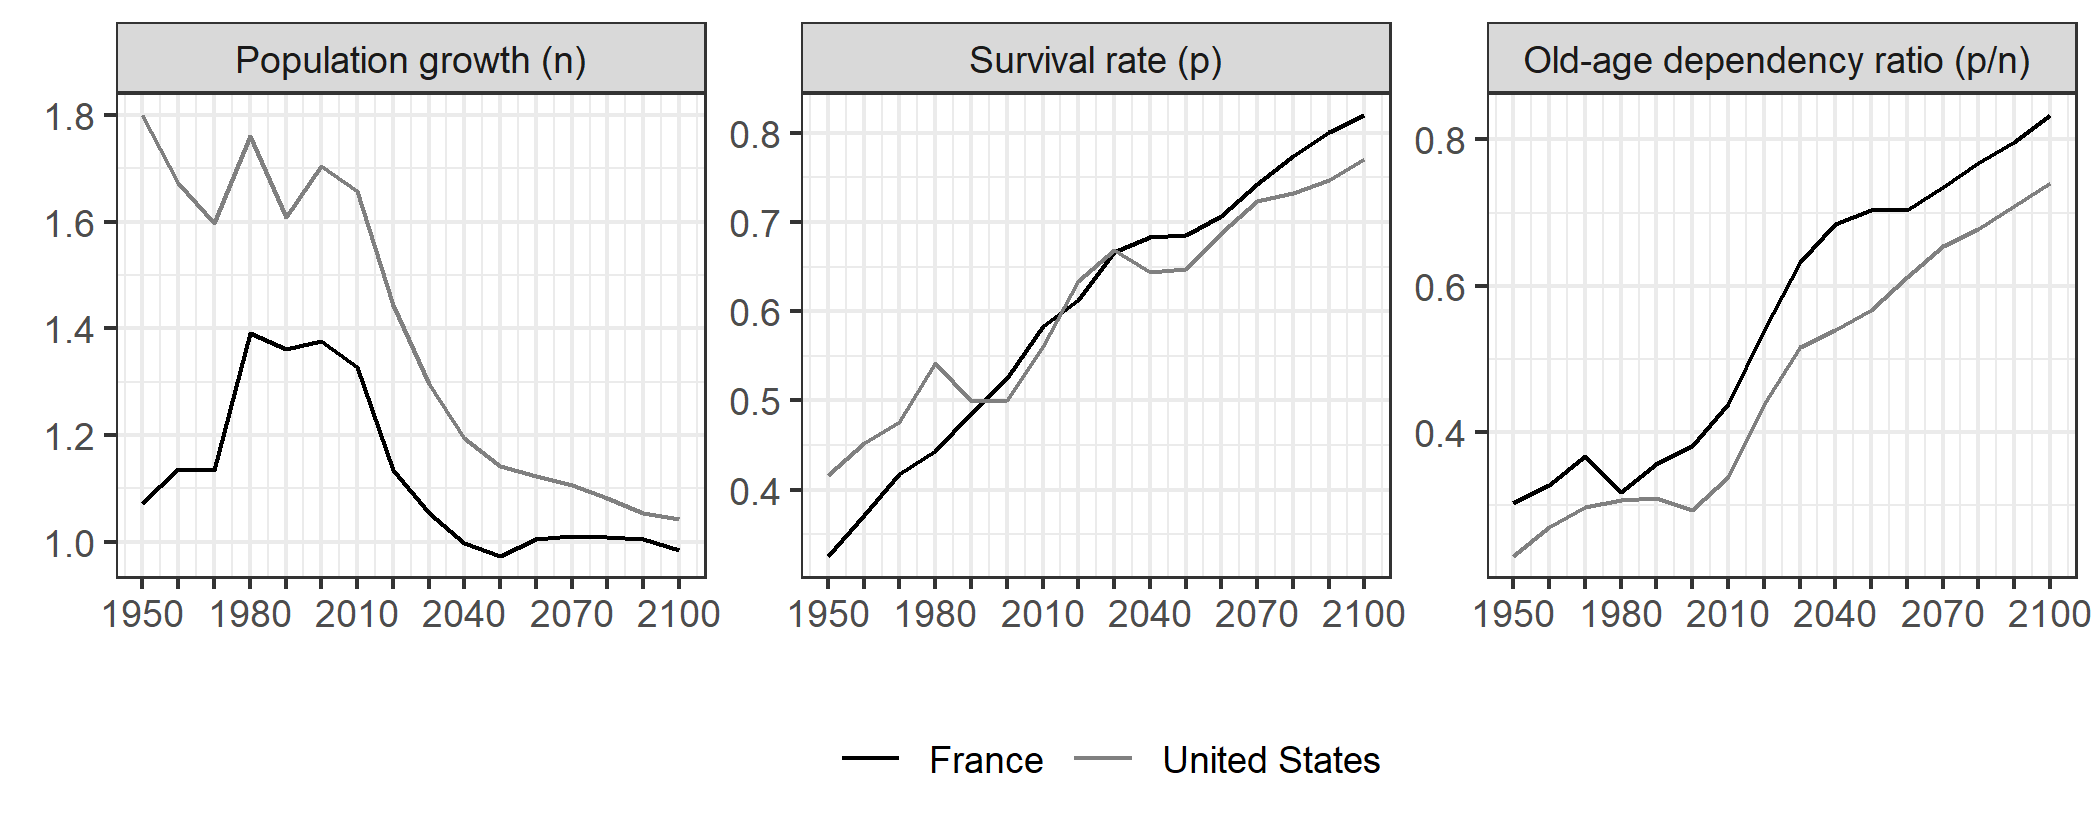
\includegraphics[width=\linewidth]{chap1/graphic/quant-demo.png}
	\vspace{-3em}
	\justify\singlespacing\footnotesize\textit{Notes:} The figure displays, for each country every 10 years, the population growth rate, the survival rate and the old-age dependency ratio. Data correspond to the ``medium variant'' estimates from the  \href{https://population.un.org/wpp/}{United Nations World Population Prospects 2017}.
\end{figure}
I distinguish three eras in terms of dynamics that correspond to the life cycle of the boomers' generation: when the boomers are young between 1970 and 2010; when they retire; and thereafter once they disappeared. Until 2010, the old-age dependency ratio remains roughly stable due to the massive entry of the boomers into the labor force that offsets the rise in the survival rate due to increasing life expectancy. Thereafter, as the boomer generation retires, the survival rate continues to grow and population growth declines. As a consequence, the old-age dependency ratio explodes.

\textbf{Labor share.} I use labor share data from the \href{https://www.rug.nl/ggdc/productivity/pwt/}{Penn World Table 10.0} (PWT); see \citet{Feenstra2015Next} for more details on these data. In this dataset, the labor share $\theta_t$ corresponds to the share of labor compensation in GDP. As argued by \citet{Gollin2002Getting}, the measurement of the labor share is influenced by the adjustment method to take into account self-employed income. In the theoretical framework, workers are young individuals and supply only labor. In line with the model, I consider self-employed income as labor compensation.

\textbf{Capital stock.} I use the capital stock at constant 2011 national prices from the PWT for the capital stock $K_t$. To disentangle the effect of changes in the number of hours worked, I adjust both variables by the average annual hours worked by persons engaged from the same data source.

\textbf{Labor and unemployment.} I also use the number of persons in employment from the PWT. In the model, labor supply is inelastic and there is no distinction between unemployed and inactive individuals. The unemployed, in terms of the model specification, correspond to all agents that do not work. However, in high-income countries such as France and the United States, inactive people also benefit from redistribution through transfer payments. Therefore, I treat them as unemployed and the redistribution is captured through unemployment benefit $b_t$ in the model. I compute the unemployment rate such that $u_t = 1 - emp_t/N^{15-64}_t$, where $emp_t$ is the number of persons in employment and $N_t^{15-64}$ is the working-age population.\footnote{I consider the whole working-age population instead of the young population. Due to the demographic specification of the model, young agents correspond to those between 20 and 60 years old. Data on the number of persons engaged per age group are not available in PWT. Therefore, taking only $N^y_t$ as denominator would bias downward the unemployment rate. % Results are robust to different specifications of the unemployment rate.
Although there are other sources of population data, I rely on the PWT to have consistency using the same data source for input factors and output.}
Then, I compute labor according to the identity $L_t\equiv(1-u_t)N_t^y$.

\textbf{Public policy variables.} I use the government revenue as a share of GDP from the \href{https://www.oecd.org/tax/tax-policy/tax-database/}{OECD Tax Database} to proxy the tax rate $\tau_t$, these data are not available before 1970. I use the pension spending expressed in percentage of GDP as a measure of the old-age specific government spending, i.e. $g_tN^o_t/Y_t$, as it is likely to be positively correlated with. Lastly, I consider the public unemployment spending expressed in percentage of GDP for the share of total unemployment benefits, i.e. $b_tu_tN^y_t/Y_t$. Both latter variables are from the OECD data.

\textbf{Normalization.} 
I normalize the capital-labor ratio $k_t$ and the young population $N_t^y$ to their 1950 values. $L_t$ is computed such that the unemployment rate $u_t$ matches the one derived for 1950 and $K_t$ satisfies the identity $k_t \equiv K_t/L_t$.

\subsection{Calibration}\label{chap1-calibration}

% Calibration
Once stock variables are normalized, I calibrate the parameters of the model $\{ \alpha,$ $\phi,$ $\sigma,$ $\omega,$ $\beta,$ $A \}$. Table \ref{chap1-tab:quant-param} summarizes parameters for both countries.
\begin{table}[!tb]
    \centering
    \begin{threeparttable}
        \caption{Parameters} \label{chap1-tab:quant-param}
        
\begin{tabular}{llrrl}
\toprule
\textbf{} & \textbf{Parameter} & \textbf{France} & \textbf{US} & \textbf{Target}\\
\midrule
$\alpha$ & Discount rate & 0.669 & 0.669 & Set to $0.99^{40}$\\
$\phi$ & Capital share in 1950 & 0.232 & 0.323 & $1-\theta_{1950}$\\
$\sigma$ & Capital-labor elasticity of substitution & 1.206 & 1.270 & Estimation\\
$\omega$ & Relative ideological spread-out & 1.103 & 0.622 & $k_{1970}$\\
$\beta$ & Preference for old-age specific gov. spending & 0.570 & 0.002 & $\tau_{1970}$\\
$A$ & Scale parameter of the production function & 127.782 & 18.430 & $\theta_{1990}$\\
\bottomrule
\end{tabular}

        \begin{tablenotes}[flushleft]
            \footnotesize\item \textit{Notes}: The table reports the parameters and the targets from the calibration of the model for France and the United States. The discount rate is set to 0.99 on annual basis. The capital share in 1950 matches the labor share in the same year.
            The capital-labor elasticity of substitution is obtained with a single-equation estimation from the two first-order conditions of the profit maximization with normalized CES production function.
            The relative ideological spread-out matches the capital-labor ratio in 1970, the preference for old-age specific government spending matches the tax rate in 1970, and the scale parameter of the production function matches the labor share in 1990.
        \end{tablenotes}
    \end{threeparttable}
\end{table}
I set the discount rate $\alpha$ at 0.669, i.e. 0.99 on annual basis. 
The parameter $\phi$ corresponds to the capital share in 1950 and is derived from the labor share in the same year. 

The main parameter of the model is the elasticity of substitution between capital and labor, i.e. $\sigma$. I follow the specification of \citet{Klump2007Factor} for a CES production function with biased technical change. % \textit{à la} \citet{David1965Biased}. 
I estimate $\sigma$ with a single-equation estimation from the two first-order conditions of the profit maximization, namely,
\begin{equation} \label{chap1-eq:est-sigma}
	\ln \Theta_t = \gamma_0 + \gamma_1 \ln (k_t/k_0) + \gamma_2\left(t-t_0\right),
\end{equation}
where $\gamma_0$ is the intercept, $\gamma_1\equiv(1-\sigma)/\sigma$ encompasses the elasticity of substitution between both factors, and $\gamma_2$ captures the overall bias in technical change.

Table \ref{chap1-tab:sigma-estimate-short} summarizes the coefficients and provides the estimated elasticity for both countries.
\begin{table}[!tb]
    \centering
    \caption{Estimation of the capital-labor elasticity of substitution} \label{chap1-tab:sigma-estimate-short}
    \begin{threeparttable}
        \setlength{\tabcolsep}{12pt}
        \begin{tabular}{l D{.}{.}{2.6} D{.}{.}{2.6} D{.}{.}{2.6} D{.}{.}{2.6}}
\toprule
 & \multicolumn{4}{c}{Linear regression - OLS} \\
\cmidrule(lr){2-5}
 & \multicolumn{2}{c}{France} & \multicolumn{2}{c}{United States} \\
\cmidrule(lr){2-3}\cmidrule(lr){4-5}
 & \multicolumn{1}{c}{(1)} & \multicolumn{1}{c}{(2)} & \multicolumn{1}{c}{(1)} & \multicolumn{1}{c}{(2)} \\
\midrule
$\gamma_1$ & 1.233^{***}  & 1.214^{***}  & 0.752^{***}  & 0.762^{***}  \\
           & (0.020)      & (0.019)      & (0.012)      & (0.014)      \\
$\gamma_2$ & -0.318^{***} & -0.171^{***} & -0.213^{***} & -0.363^{***} \\
           & (0.014)      & (0.043)      & (0.017)      & (0.101)      \\
$\gamma_3$ &              & -0.005^{***} &              & 0.002        \\
           &              & (0.001)      &              & (0.002)      \\
\midrule
$\sigma$ & \multicolumn{1}{c}{1.466} & \multicolumn{1}{c}{1.206} & \multicolumn{1}{c}{1.270} & \multicolumn{1}{c}{1.571} \\
\midrule
R$^2$ & \multicolumn{1}{c}{0.891} & \multicolumn{1}{c}{0.908} & \multicolumn{1}{c}{0.703} & \multicolumn{1}{c}{0.713}\\
Adj. R$^2$ & \multicolumn{1}{c}{0.889} & \multicolumn{1}{c}{0.906} & \multicolumn{1}{c}{0.699} & \multicolumn{1}{c}{0.704}\\
Num. obs. & \multicolumn{1}{c}{69} & \multicolumn{1}{c}{69} & \multicolumn{1}{c}{70} & \multicolumn{1}{c}{70}\\
\bottomrule
\end{tabular}

        \begin{tablenotes}[flushleft]
            \footnotesize{\item\textit{Notes}: $^{***}p<0.01$; $^{**}p<0.05$; $^{*}p<0.1$. Standard errors between parentheses. The labor-to-capital income ratio (in log) is the dependent variable. The periods of the estimate correspond to 1950-2018 for France and 1950-2019 for the US. Single-equation estimation from the two first-order conditions of the profit maximization for a CES production function with biased technical change. Coefficients are as follows. $\gamma_0$ is the intercept, $\gamma_1\equiv(1-\sigma)/\sigma$ encompasses the elasticity of substitution between capital and labor, and $\gamma_2$ captures the overall bias in technical change.}
        \end{tablenotes}
    \end{threeparttable}
\end{table}
For France, the specification in column (2) that controls for the bias of technical change is the preferred one. Since $\gamma_3$ is negative and significant it means that the technical change is biased toward capital.
For the US, I consider the first specification as $\gamma_3$ is not significant in column (2). Note that the coefficients from which I derive the elasticity, i.e. $\gamma_2$, are significantly negative, implying that $\sigma$ is significantly greater than one.
I hence obtain an elasticity of 1.206 for France and 1.270 for the United States.
Therefore, both input factors are gross substitutes. These values are in line with recent estimates in the literature on the labor share such as \citet{Karabarbounis2014Global} who use cross-sectional data on 50 countries over the period 1975-2012 to find an elasticity greater than 1, with an average of 1.28 in their baseline estimates.\footnote{\citet{Caballero1998Jobless} use a relatively high value of the capital-labor elasticity of substitution, about 6.00, to simulate French data.}

% 3 remaining parameter => match moments
To calibrate the three remaining parameters, I match three moments in the data. 
% OMEGA
The relative ideological spread-out $\omega$ is set to match the capital-labor ratio $k_t$ in 1970 using equation \eqref{chap1-eq:equilibrium-k}.
The parameter being greater in France than in the US, it suggests that young people have inherently more political weight in France compared to the US.
% BETA
The preference for old-age specific government spending $\beta$ is set to match the tax rate $\tau_t$ in 1970, from the data, using equation \eqref{chap1-eq:tax-rate}.
% beta FR > beta US
As expected, the preference for old-age specific government expenditure---relative to private consumption---is greater in France than in the United States.
% A (scale parameter)
Lastly, the scale parameter of the production function $A$ is set to match the average labor share between 1988 and 1992.

\subsection{Model predictions}\label{chap1-model_pred}

I simulate the model using the parameters values above. For the remaining of the paper, I refer to this simulation as the benchmark simulation. Figure \ref{chap1-fig:quant-bench-ls} displays the labor shares predicted by the model.
\begin{figure}[!tb]
	\centering
	\caption{Model predictions of the labor share} \label{chap1-fig:quant-bench-ls}
	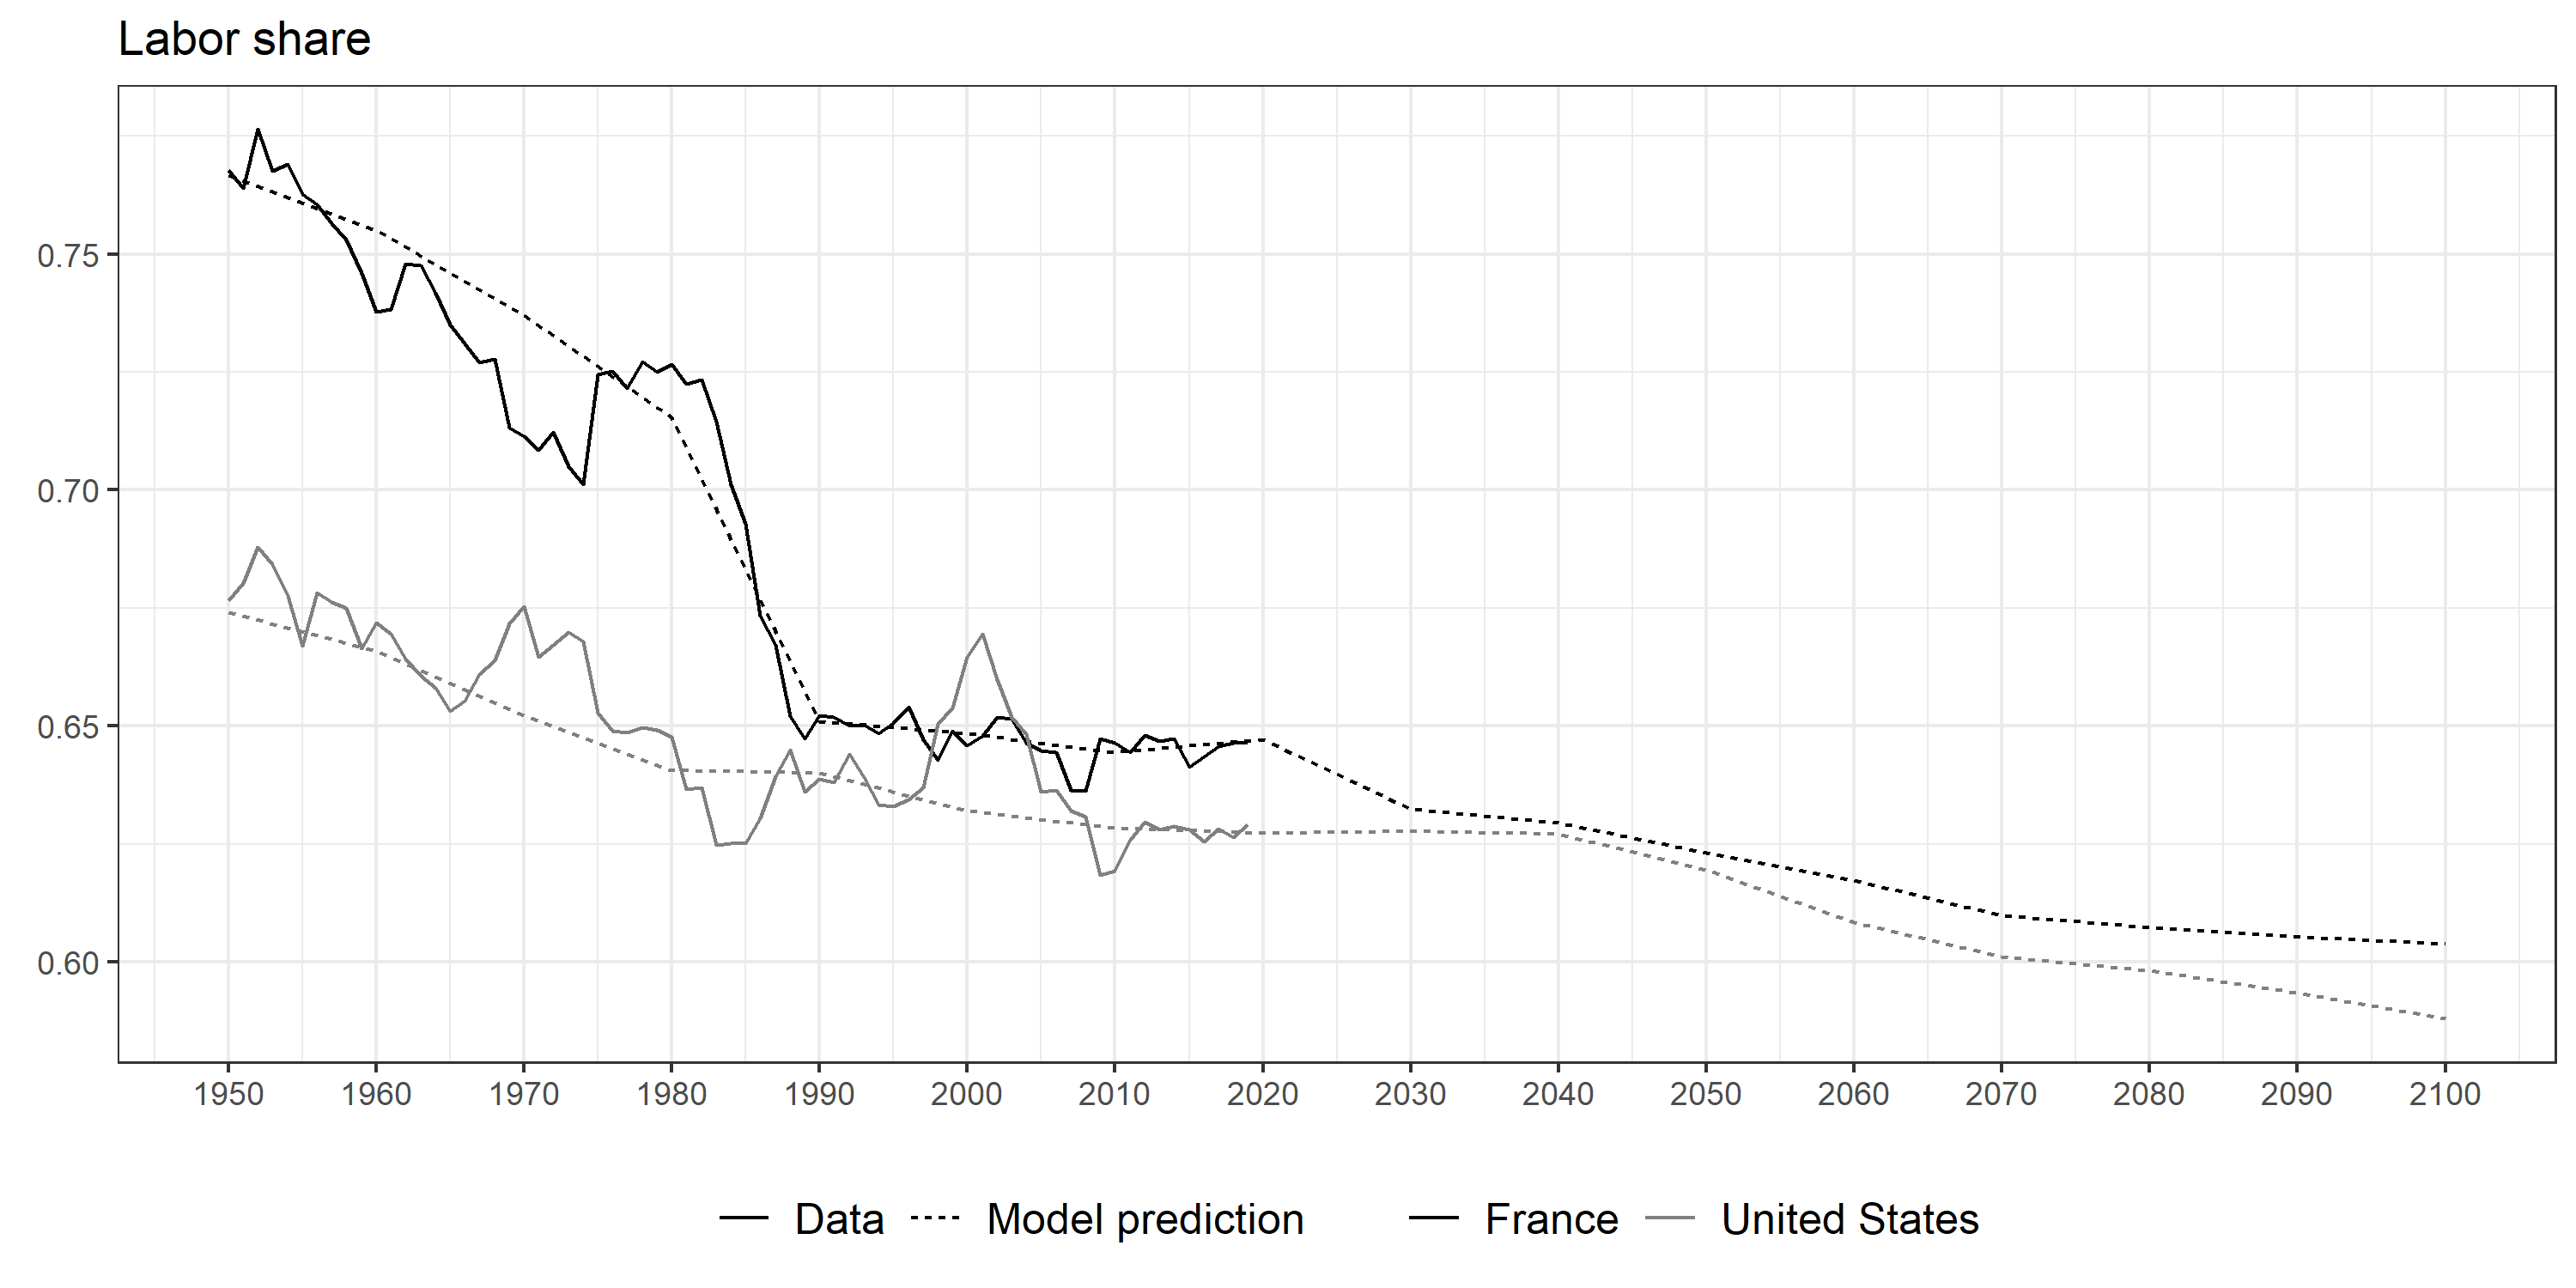
\includegraphics[width=1\linewidth]{chap1/graphic/quant-bench-ls.png}
	\vspace{-3em}
	\justify\singlespacing\footnotesize\textit{Notes:} The figure shows the labor share predictions of the model (dashed lines) and the labor share in the data (solid lines) from 1950 to 2100 for France and the US.
	Labor share data are from the \href{https://www.rug.nl/ggdc/productivity/pwt/}{Penn World Table 10.1} with self-employed income as labor compensation.
\end{figure}
The model reproduces the global trend in the data for both countries until 2020. For the US, the model underestimates the labor share around 2000. However, it captures the overall trend of the labor share over the period.
For France, model predictions are more accurate and reproduce the data since 1950. Looking at the model's predictions after 2020, the labor share should decline until the end of the century in both countries. I discuss the dynamics of variables---in the public policy equilibrium and in the labor market equilibrium---over the three periods: when the boomers are young (1970-2010), when they are retired (2010-2050), and afterward (2050-2100).

%% Other economic variables before 2010
\textbf{The young boomers (1970-2010).} 
Figure \ref{chap1-fig:quant-bench-dev7010-pub} displays the dynamics of public policy variables, expressed in percentage deviation from their 1970's value.
\begin{figure}[!tb]
	\centering
	\caption{Public policy dynamics over the 1970-2010 period} \label{chap1-fig:quant-bench-dev7010-pub}
	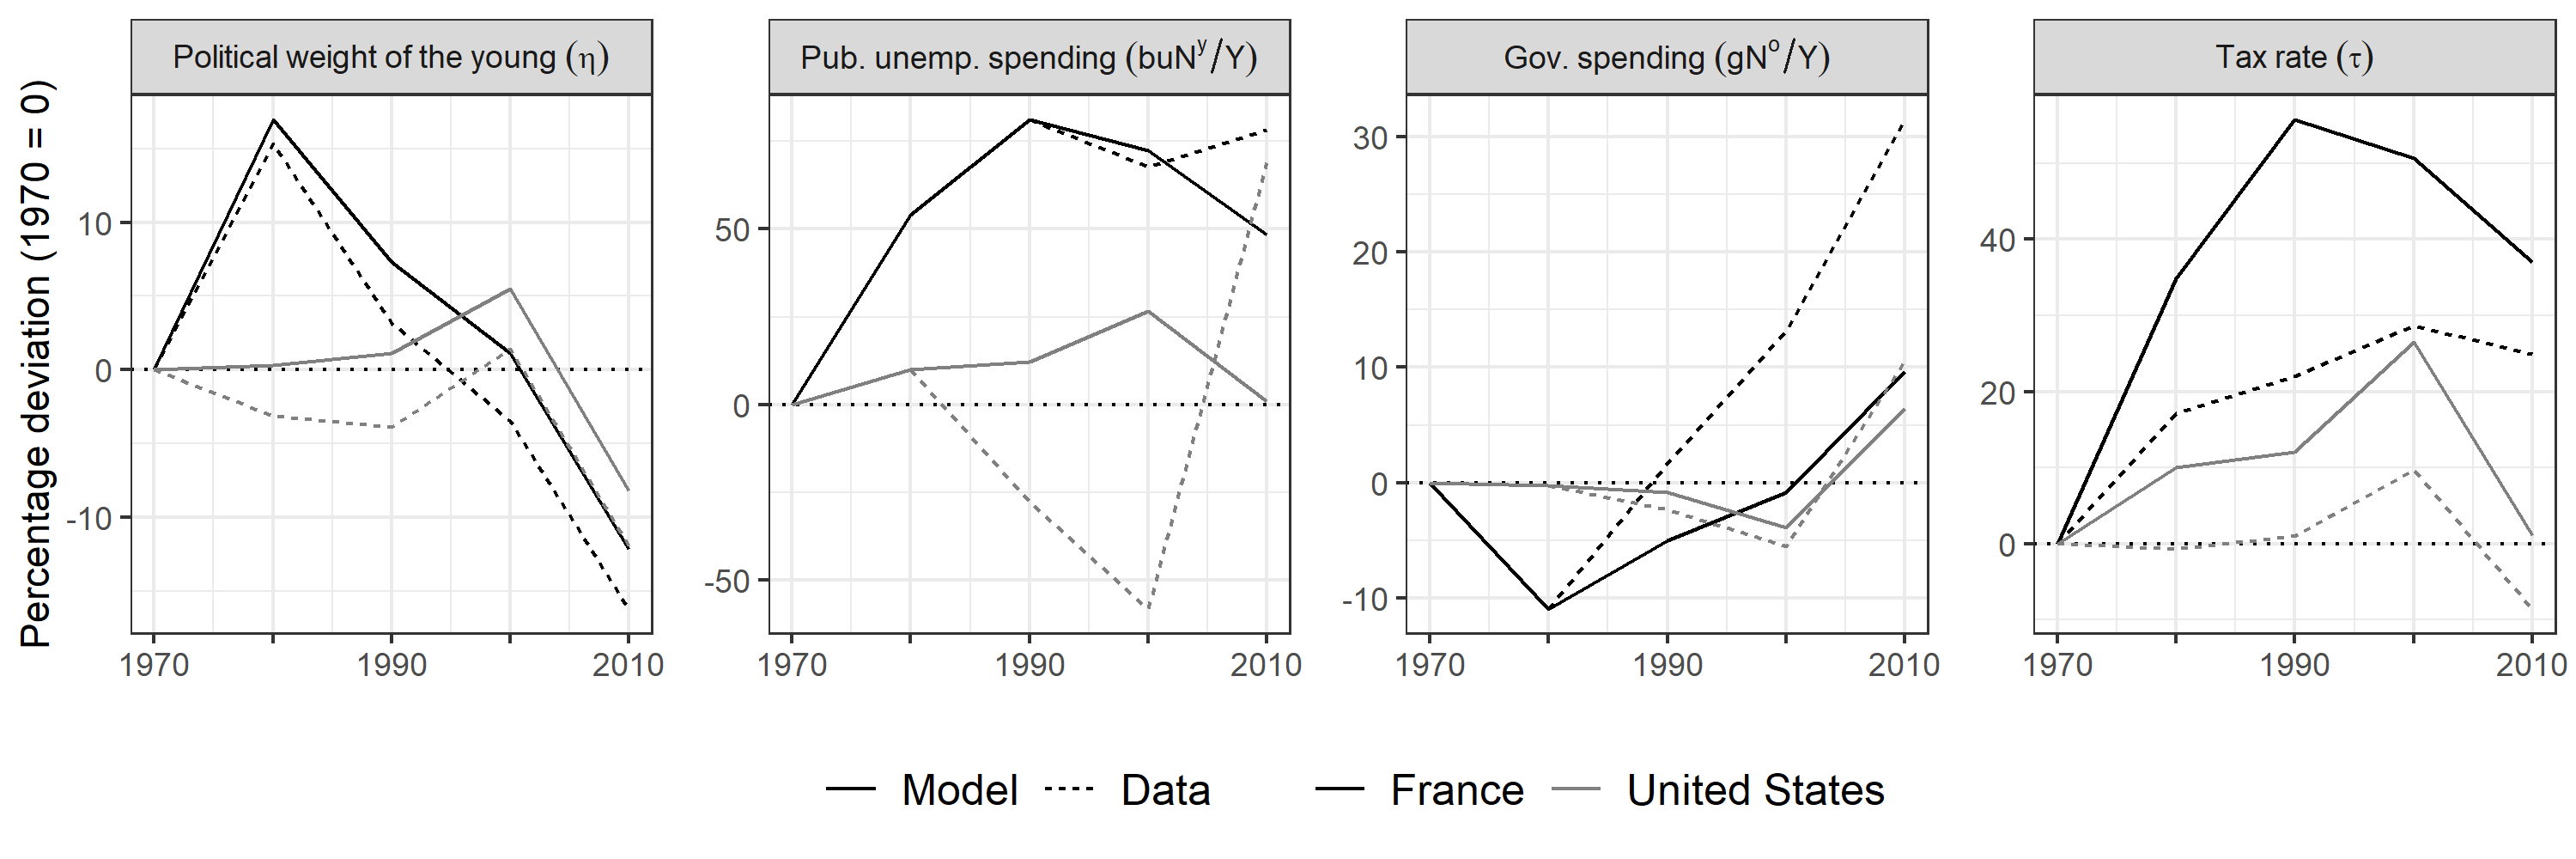
\includegraphics[width=1\linewidth]{chap1/graphic/quant-bench-dev7010-pub.png}
	\vspace{-3em}
	\justify\singlespacing\footnotesize\textit{Notes:} The figure shows the deviation of the variables from the public policy equilibrium from their 1970's value (in percentage) for France and the United States over the 1970-2010 period. Solid lines represent the dynamics obtained from the model simulation, dashed  lines represent the data, and the dotted line represents the 0-degree line.
\end{figure}
% Demographic context (n and p)
The rate of population growth $n_t$ slightly exceeds the increasing survival rate $p_t$ between 1970 and 2000. Thus, the old-age-dependency ratio $p_t/n_t$ remains roughly stable, although it declines slightly in France between 1980 and 1990 due to the massive entry of the boomers into the labor force. The old-age-dependency ratio starts to increase around 2000 due to a steady population growth combined with a sharply increasing survival rate, the boomers' generation starting to retire. As a result of this demographic context, the political weight of the young $\eta_t$ is above its 1970's level until 2000 in both countries as depicted in the first panel of the figure.

As the political weight of the young boomers rises, pro-youth policies are implemented due to the opportunistic behavior of political parties. These policies consist of more redistribution, i.e. a greater tax rate and more unemployment benefits, to prevent the income losses due to unemployment of the young boomers. Thus, the old-age specific government spending also decline, before increasing again as the boomer cohort starts to retire in 2010. Since the unemployment benefits act as an outside option for the workers, these public policy dynamics have consequences on the labor market.

Figure \ref{chap1-fig:quant-bench-dev7010-labor} displays the dynamics of labor market variables, expressed in percentage deviation from their 1970's value.
\begin{figure}[!tb]
	\centering
	\caption{Labor market dynamics over the 1970-2010 period} \label{chap1-fig:quant-bench-dev7010-labor}
	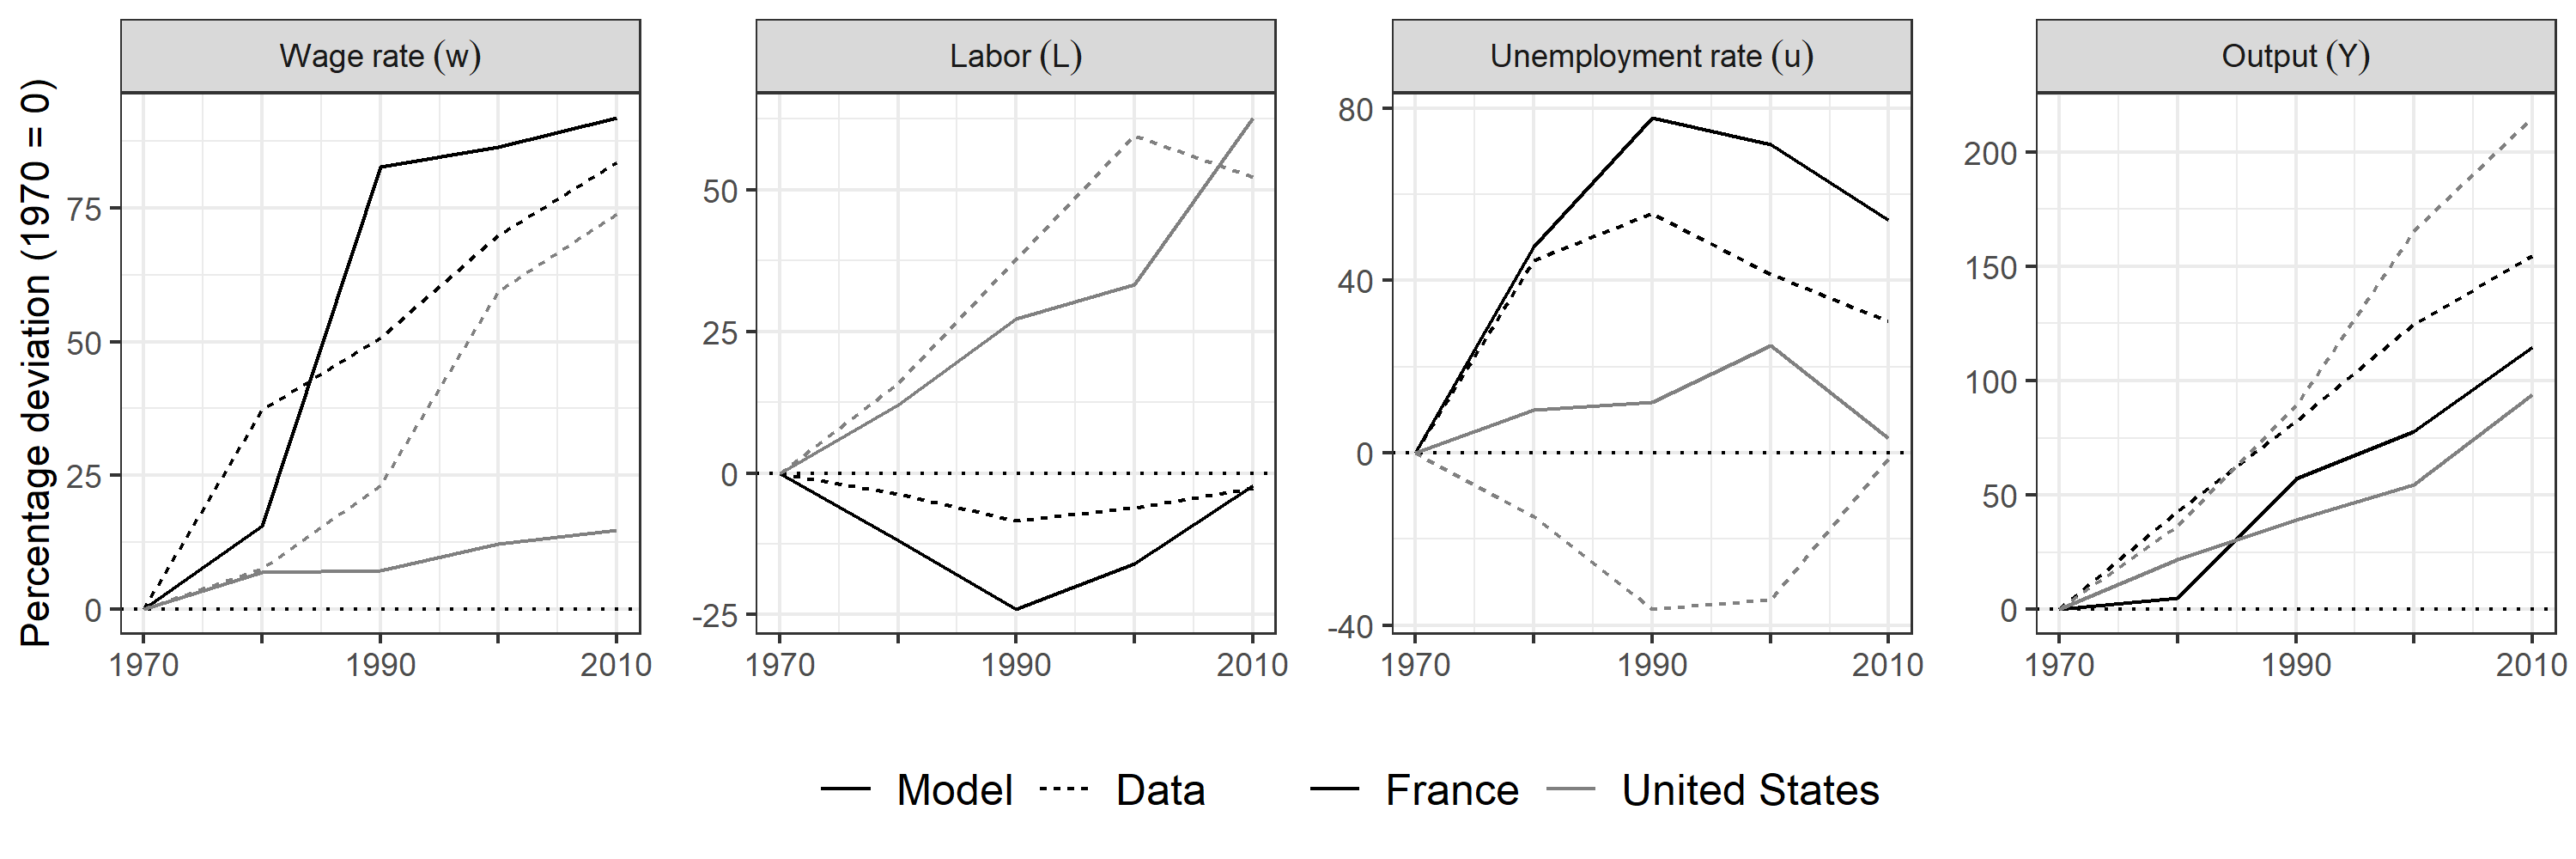
\includegraphics[width=1\linewidth]{chap1/graphic/quant-bench-dev7010-labor.png}
	\vspace{-3em}
	\justify\singlespacing\footnotesize\textit{Notes:} The figure shows the deviation of the variables from the labor market equilibrium from their 1970's value (in percentage) for France and the United States over the 1970-2010 period. Solid lines represent the dynamics obtained from the model simulation, dashed  lines represent the data, and the dotted line represents the 0-degree line.
\end{figure}
Workers can bargain greater wages as their outside option increases. Because the labor cost (i.e. the wage) increases for firms, they shift away from labor. This behavior is permitted by two features of the model. 
First, the monopsony position of the firm in the labor market enables the firm to hire and fire as much as wanted. 
Second, the capital-labor elasticity of substitution $\sigma$ is greater than one, thus, both input factors are gross substitutes and the firm is all the more able to substitute labor with capital for a given output level. This behavior leads to a decline of the number of workers $L_t$ in France and a moderate increase in the US, as highlighted in the second panel. The diverging patterns between the two countries are due to the substitution effect being stronger in France than in the US. The higher elasticity of substitution in France combined with faster growth of the capital stock $K_t$ pushes French firms to substitute relatively more labor with capital. Thus, the number of workers becomes lower than its 1970's level in France, whereas the US manage to slightly increase their labor factor because the increase in wages is not as strong as in France.

This fall in employment raises unemployment in France, the effect being enhanced by the labor force growth due to the number of young boomers. For the US, the moderate increase in labor does not manage to offset population growth. Therefore, the unemployment rate also raises as depicted in the third panel. Since both factors are gross substitutes, output $Y_t$ and output-per-worker grow along with capital-per-worker. The increase in output per worker exceeds the one of the wages, and as a result, the labor share declines.

The mechanisms until 2010 can be summarized as follows. The young boomers change labor market institutions in their favor due to their relatively high political weight. This raises the outside option of workers and hence their bargaining power, enabling them to bargain greater wages. Labor becoming costly, firms decide to shift away toward capital. This shift-away from labor engenders an increase in output-per-worker that exceeds the wage gain; thus, the labor share declines. 

\textbf{The retired boomers (2010-2050) and afterward (2050-2100).} Dynamics of the same set of variables also help to highlight the mechanisms of the model's predictions for the labor share after 2010.
Figure \ref{chap1-fig:quant-bench-dev1000-pub} displays the dynamics of public policy variables, expressed in percentage deviation from their 2010's value.
\begin{figure}[!tb]
	\centering
	\caption{Public policy dynamics over the 2010-2100 period} \label{chap1-fig:quant-bench-dev1000-pub}
	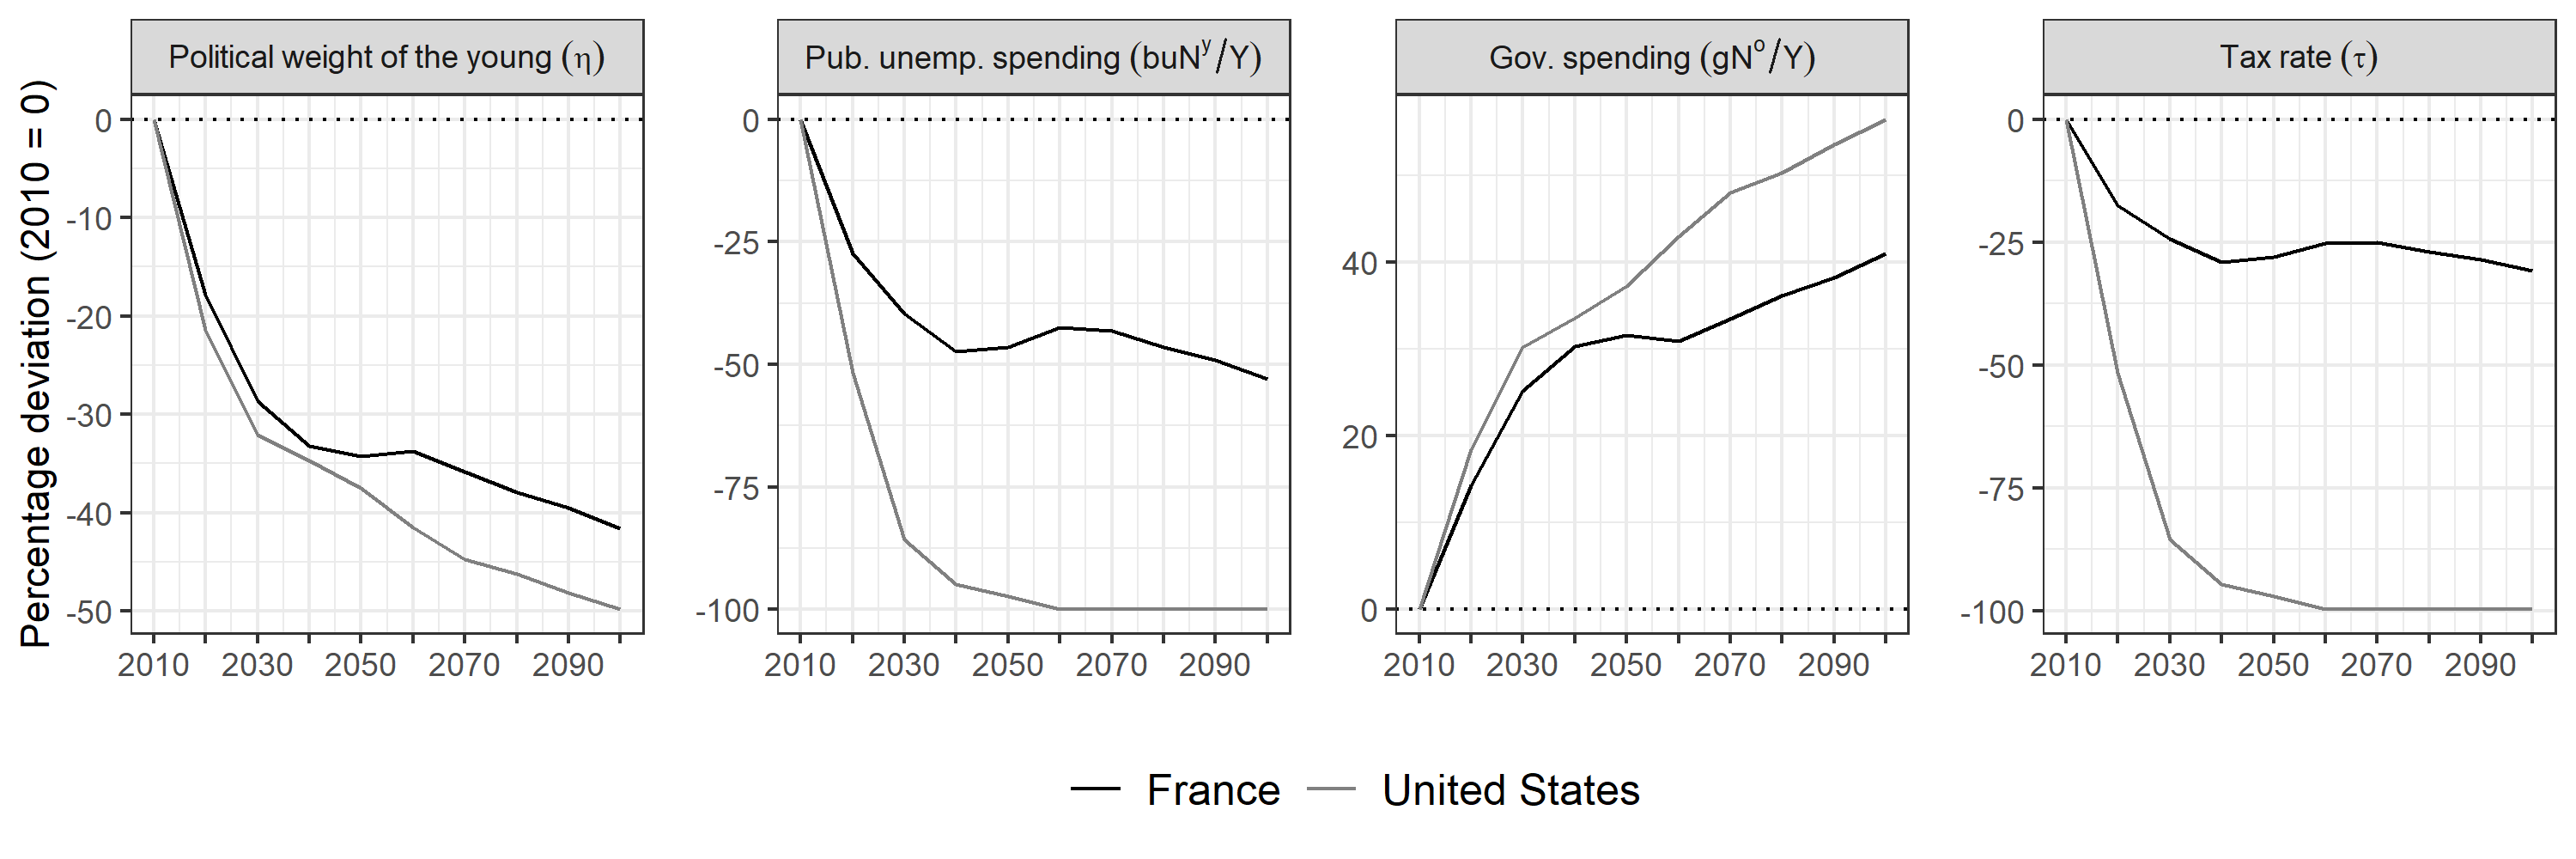
\includegraphics[width=1\linewidth]{chap1/graphic/quant-bench-dev1000-pub.png}
	\vspace{-3em}
	\justify\singlespacing\footnotesize\textit{Notes:} The figure shows the deviation of the variables from the public policy equilibrium from their 2010's value (in percentage) for France and the United States over the 2010-2100 period. Solid lines represent the dynamics obtained from the model simulation and the dotted line represents the 0-degree line.
\end{figure}
The demographic context over this period is the following: the rate of population growth $n_t$ declines sharply between 2010 and 2050 before stabilizing thereafter. Meanwhile, the survival rate $p_t$ grows by around 4\% per decade. Thus, the old-age-dependency ratio sharply increases from 2010 to 2050. Once the rate of population growth becomes stable, the old-age-dependency ratio still grows but at a lower rate. As a result, the political weight of the young, $\eta_t$, never returns to its 2010 level and strongly declines until 2050 for both countries as shown in the first panel.

As the political weight of the young declines, the reverse of the mechanism that led to the decline of the labor share when the boomers were young is expected. Opportunistic political parties favor the retired boomers and implement pro-elderly public policies, i.e. a lower tax rate and more old-age specific government spending. Thus, unemployment benefits decline and so does the outside option of workers. These changes in public policy have consequences on the labor market.

Figure \ref{chap1-fig:quant-bench-dev1000-labor} displays the dynamics of public policy variables, expressed in percentage deviation from their 2010's value.
\begin{figure}[!tb]
	\centering
	\caption{Labor market dynamics over the 2010-2100 period} \label{chap1-fig:quant-bench-dev1000-labor}
	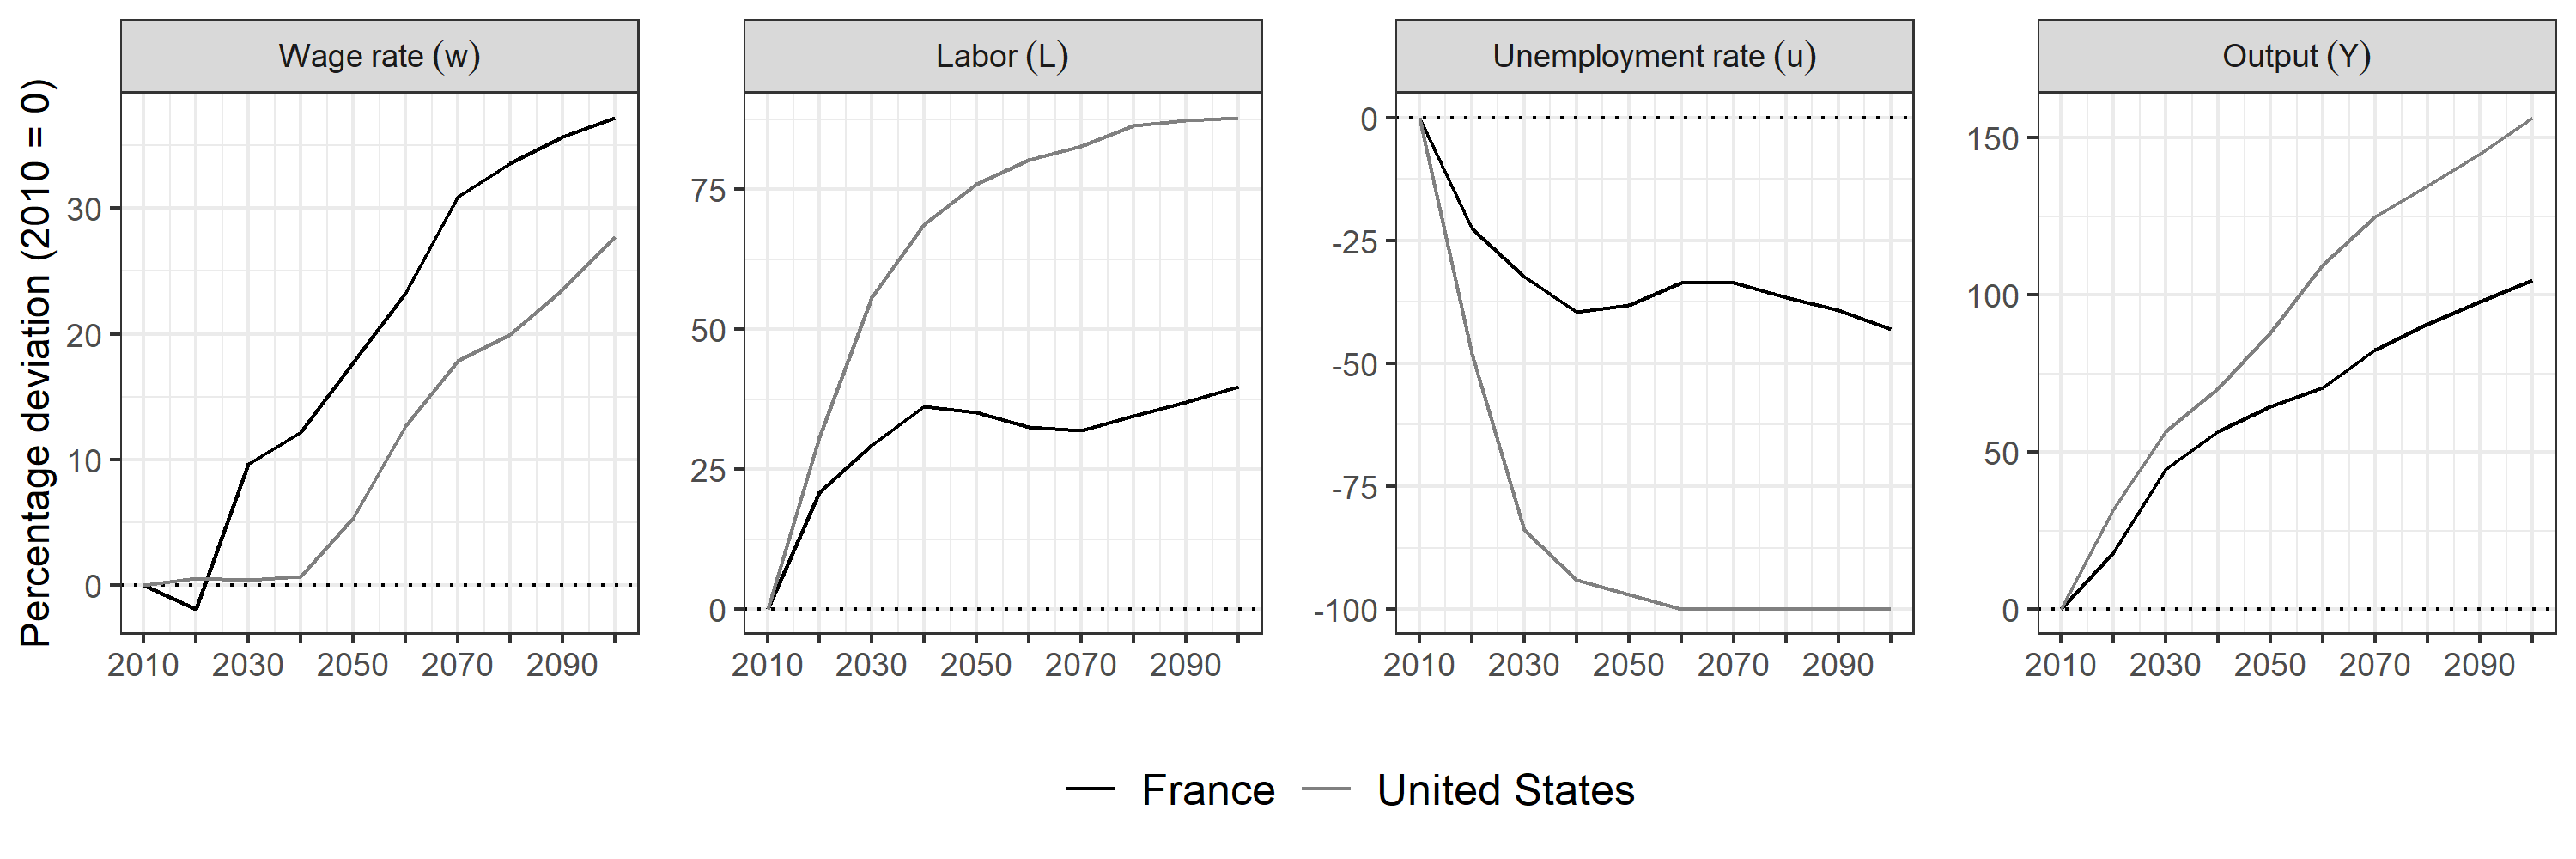
\includegraphics[width=1\linewidth]{chap1/graphic/quant-bench-dev1000-labor.png}
	\vspace{-3em}
	\justify\singlespacing\footnotesize\textit{Notes:} The figure shows the deviation of the variables from the labor market equilibrium from their 2010's value (in percentage) for France and the United States over the 2010-2100 period. Solid lines represent the dynamics obtained from the model simulation and the dotted line represents the 0-degree line.
\end{figure}
As a result, they concede a wage stagnation inciting firms to hire more, as depicted in the second panel. The unemployment rate drops due to higher employment combined with the decline of the rate of population growth, as shown in the third panel.

Nonetheless, the labor share never recovers its 2010's level. The dynamics of the labor share are governed by two factors: an increase in employment and a higher capital stock arising from the savings of the boomers when they were young. These savings were fostered by the size of the boomer generation; the rising expected life expectancy; and the high level of their wages. While higher employment tends to increase the labor share, the larger stock of capital tends to reduce it, keeping the labor share roughly stable in both countries when the boomers are retired.

Once the boomers pass away, after 2050, the decline in the political power of the young slows down in both countries. This slowdown allows workers to bargain greater wages. French firms substitute labor with capital to thwart workers' appropriation of the rents, leading to a decline of the labor factor and so a rise in unemployment. On the other side of the Atlantic, firms in the US manage to hire until full-employment due to the sharp increase in capital and the stagnation of the labor supply. However, the wage gains remain lower than the rise in output-per-worker in both countries. Therefore, both labor shares decline to reach 60.4\% in France and 58.8\% in the US by 2100, while their respective levels were about 64.5\% and 62.8\% in 2010.

The mechanisms after 2010 can be summarized as follows. The boomers retire and change the public policy in their favor, reducing taxes and unemployment benefits which raises employment. The positive effect of employment on the labor share is dampened by capital accumulation due to the extensive savings of the boomers when they were young. Consequently, the labor share slightly increases in France and stabilizes in the US, before declining again by the end of the century due to the aging of the population.

\subsection{Factor-accumulation and policy-mechanism effects} \label{chap1-counterfactual}

% Mechanisms so far
So far I have highlighted the different mechanisms through which the age structure of the population affects economic variables and therefore the labor share. Demographic changes are due to changes in two exogenous variables: the population growth rate $n_t$ and the survival rate $p_t$. 
Their dynamics may affect the labor share through two channels: the \textit{direct factor-accumulation} effect and the \textit{indirect policy-mechanism} effect.

% Quantify
To quantify the respective role of each effect, I make counterfactual simulations. In these simulations, I neutralize a channel of demographic changes by setting it to its level in 1970, i.e. the decade before the massive entry of the boomers on the labor market.
% Initial values
Table \ref{chap1-tab:quant-demo70} summarizes the demographic variables in 1970.
\begin{table}[!tb]
    \centering
    \begin{threeparttable}
        \caption{Demographic variables in 1970} \label{chap1-tab:quant-demo70}
        
\begin{tabular}{llrr}
\toprule
\textbf{} & \textbf{Variable} & \textbf{France} & \textbf{United States}\\
\midrule
$n_{1970}$ & Population growth rate & 1.134 & 1.597\\
$p_{1970}$ & Survival rate & 0.417 & 0.476\\
$p_{1990}$ & Expected survival rate & 0.583 & 0.561\\
$\frac{p_{1970}}{n_{1970}}$ & Old-age dependency ratio & 0.368 & 0.298\\
$\eta_{1970}$ & Young political weight of the young & 4.169 & 2.869\\
\bottomrule
\end{tabular}

        \begin{tablenotes}[flushleft]
            \footnotesize{\item \textit{Notes}: The table reports the demographic variables in 1970 for France and the United States. 
            % Data are from the benchmark simulation of the model.
            }
        \end{tablenotes}
    \end{threeparttable}
\end{table}
Then, I compare counterfactual simulations to the benchmark obtained in section \ref{chap1-model_pred}, thus, I quantify to which extent each channels affect the labor share. For more details on the methodology to construct the counterfactual simulations, see appendix \ref{chap1-countermetho}.

% Direct vs indirect
To neutralize the factor accumulation effect, I suppose that all demographic parameters remain at their 1970's level, i.e. $n^\prime_t = n_{1970}$ and $p^\prime_t = p^\prime_{t+1} = p_{1970}$, which affects population dynamics and the saving rate. In this simulation, only the political weight of the young remains identical to the benchmark simulation, i.e. $\eta_t^\prime = \eta_t$. Conversely, I neutralize the policy mechanism effect by setting the political weight of the young to its level in 1970, i.e. $\eta^\prime_t = \eta_{1970}$, while all demographic parameters remain at their benchmark values. Lastly, I make a counterfactual simulation to neutralize both channels in which $n^\prime_t = n_{1970}$, $p^\prime_t = p^\prime_{t+1} = p_{1970}$ and $\eta_t^\prime = \eta_{1970}$. This latter simulation is the baseline counterfactual simulation.

% Figure for direct vs indirect
Figure \ref{chap1-fig:quant-decomp-channel} presents the sizes of the factor accumulation effect and the policy mechanism effect, derived from the counterfactual simulations, in percentage points.
\begin{figure}[!tb]
	\centering
	\caption{Decomposition of the channels of demographic changes} \label{chap1-fig:quant-decomp-channel}
	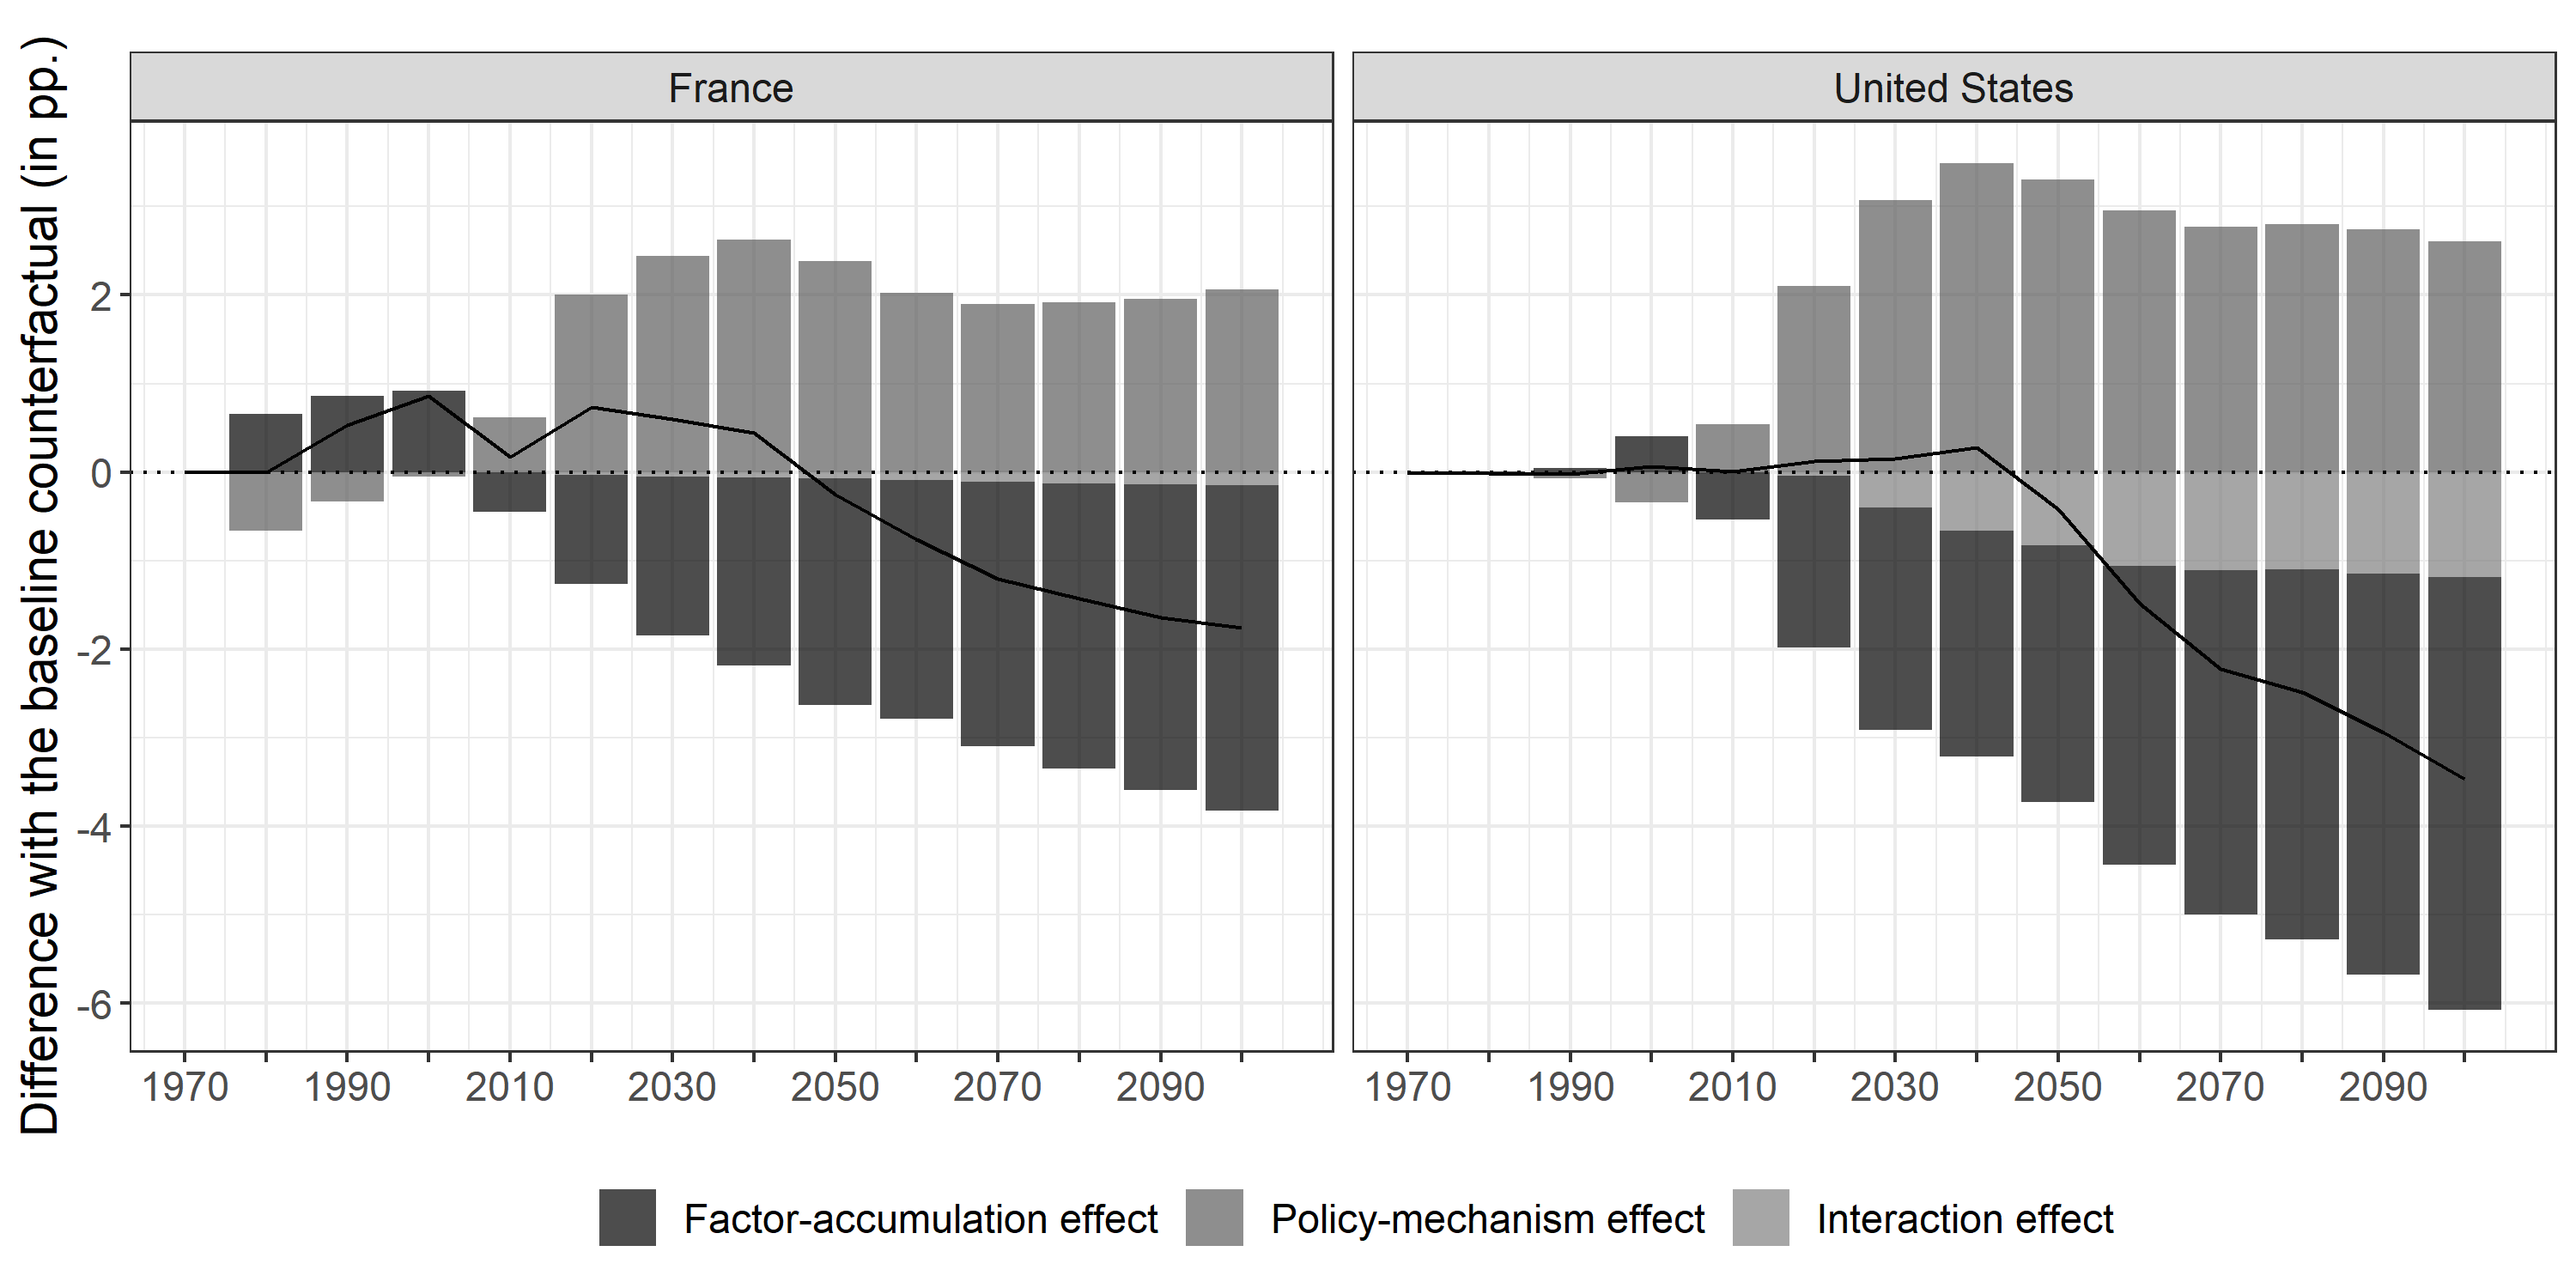
\includegraphics[width=1\linewidth]{chap1/graphic/quant-decomp-channel.png}
	\vspace{-3em}
	\justify\singlespacing\footnotesize\textit{Notes:} The figure shows the decomposition of the channels of demographic changes on the labor share. Effects are expressed in percentage point difference with the baseline counterfactual simulation. The baseline counterfactual corresponds to the simulation where all the demographic variables and the young political weight remain at their initial levels. The factor-accumulation effect accounts for the effect of demographic changes through the factor-accumulation channel on the labor share, while the policy-mechanism effect accounts for the effect of demographic changes through the policy-mechanism channel. Both effects are obtained by taking the difference between the benchmark labor share and the labor share from the simulation in which the channel is canceled. The interaction effect is defined as the part which is not exclusively explained by both effects independently. The solid line represents the net effect corresponding to the sum of the three effects, that is also the difference between the labor shares from the benchmark and the baseline counterfactual simulation.
\end{figure}
% Direct mostly positive % Increasing Ny => low wages => increases L
The factor-accumulation effect is mostly positive when the boomers are young, because the increasing labor supply is in favor of firms within the bargaining, keeping wages low which fosters employment. 
% In addition, the saving rate remains low and so does the capital stock.
Meanwhile, the policy-mechanism effect harms the labor share, owing to the rise of the young boomers' political weight which increases their unemployment benefits, hence wages, and therefore incites firms to shift away from labor toward capital.

% AFTER 2010: boomers retire, both effects are reversed
Once the boomers start to retire in 2010, both effects are reversed. The policy-mechanism effect becomes positive because old boomers foster pro-elderly public policy. This change in the policy is done at the cost of labor market insurance. Thus, workers are not able to bargain greater wages which fosters labor demand. Nonetheless, the factor-accumulation effect is negative because of the large amount of available capital stock due to the savings of the boomers when they were young. As a result, the factor-accumulation effect offsets the positive impact on the labor share of the reversal policy-mechanism effect.

% % \textbf{Summary of the effects.} 
% Figure \ref{chap1-fig:quant-decomp-sum} summarizes the relative share of the effects of demographic changes on the labor share by period and country.
% \begin{figure}[!tb]
% 	\centering
% 	\caption{Relative share of the effects of demographic changes on the labor share} \label{chap1-fig:quant-decomp-sum}
% 	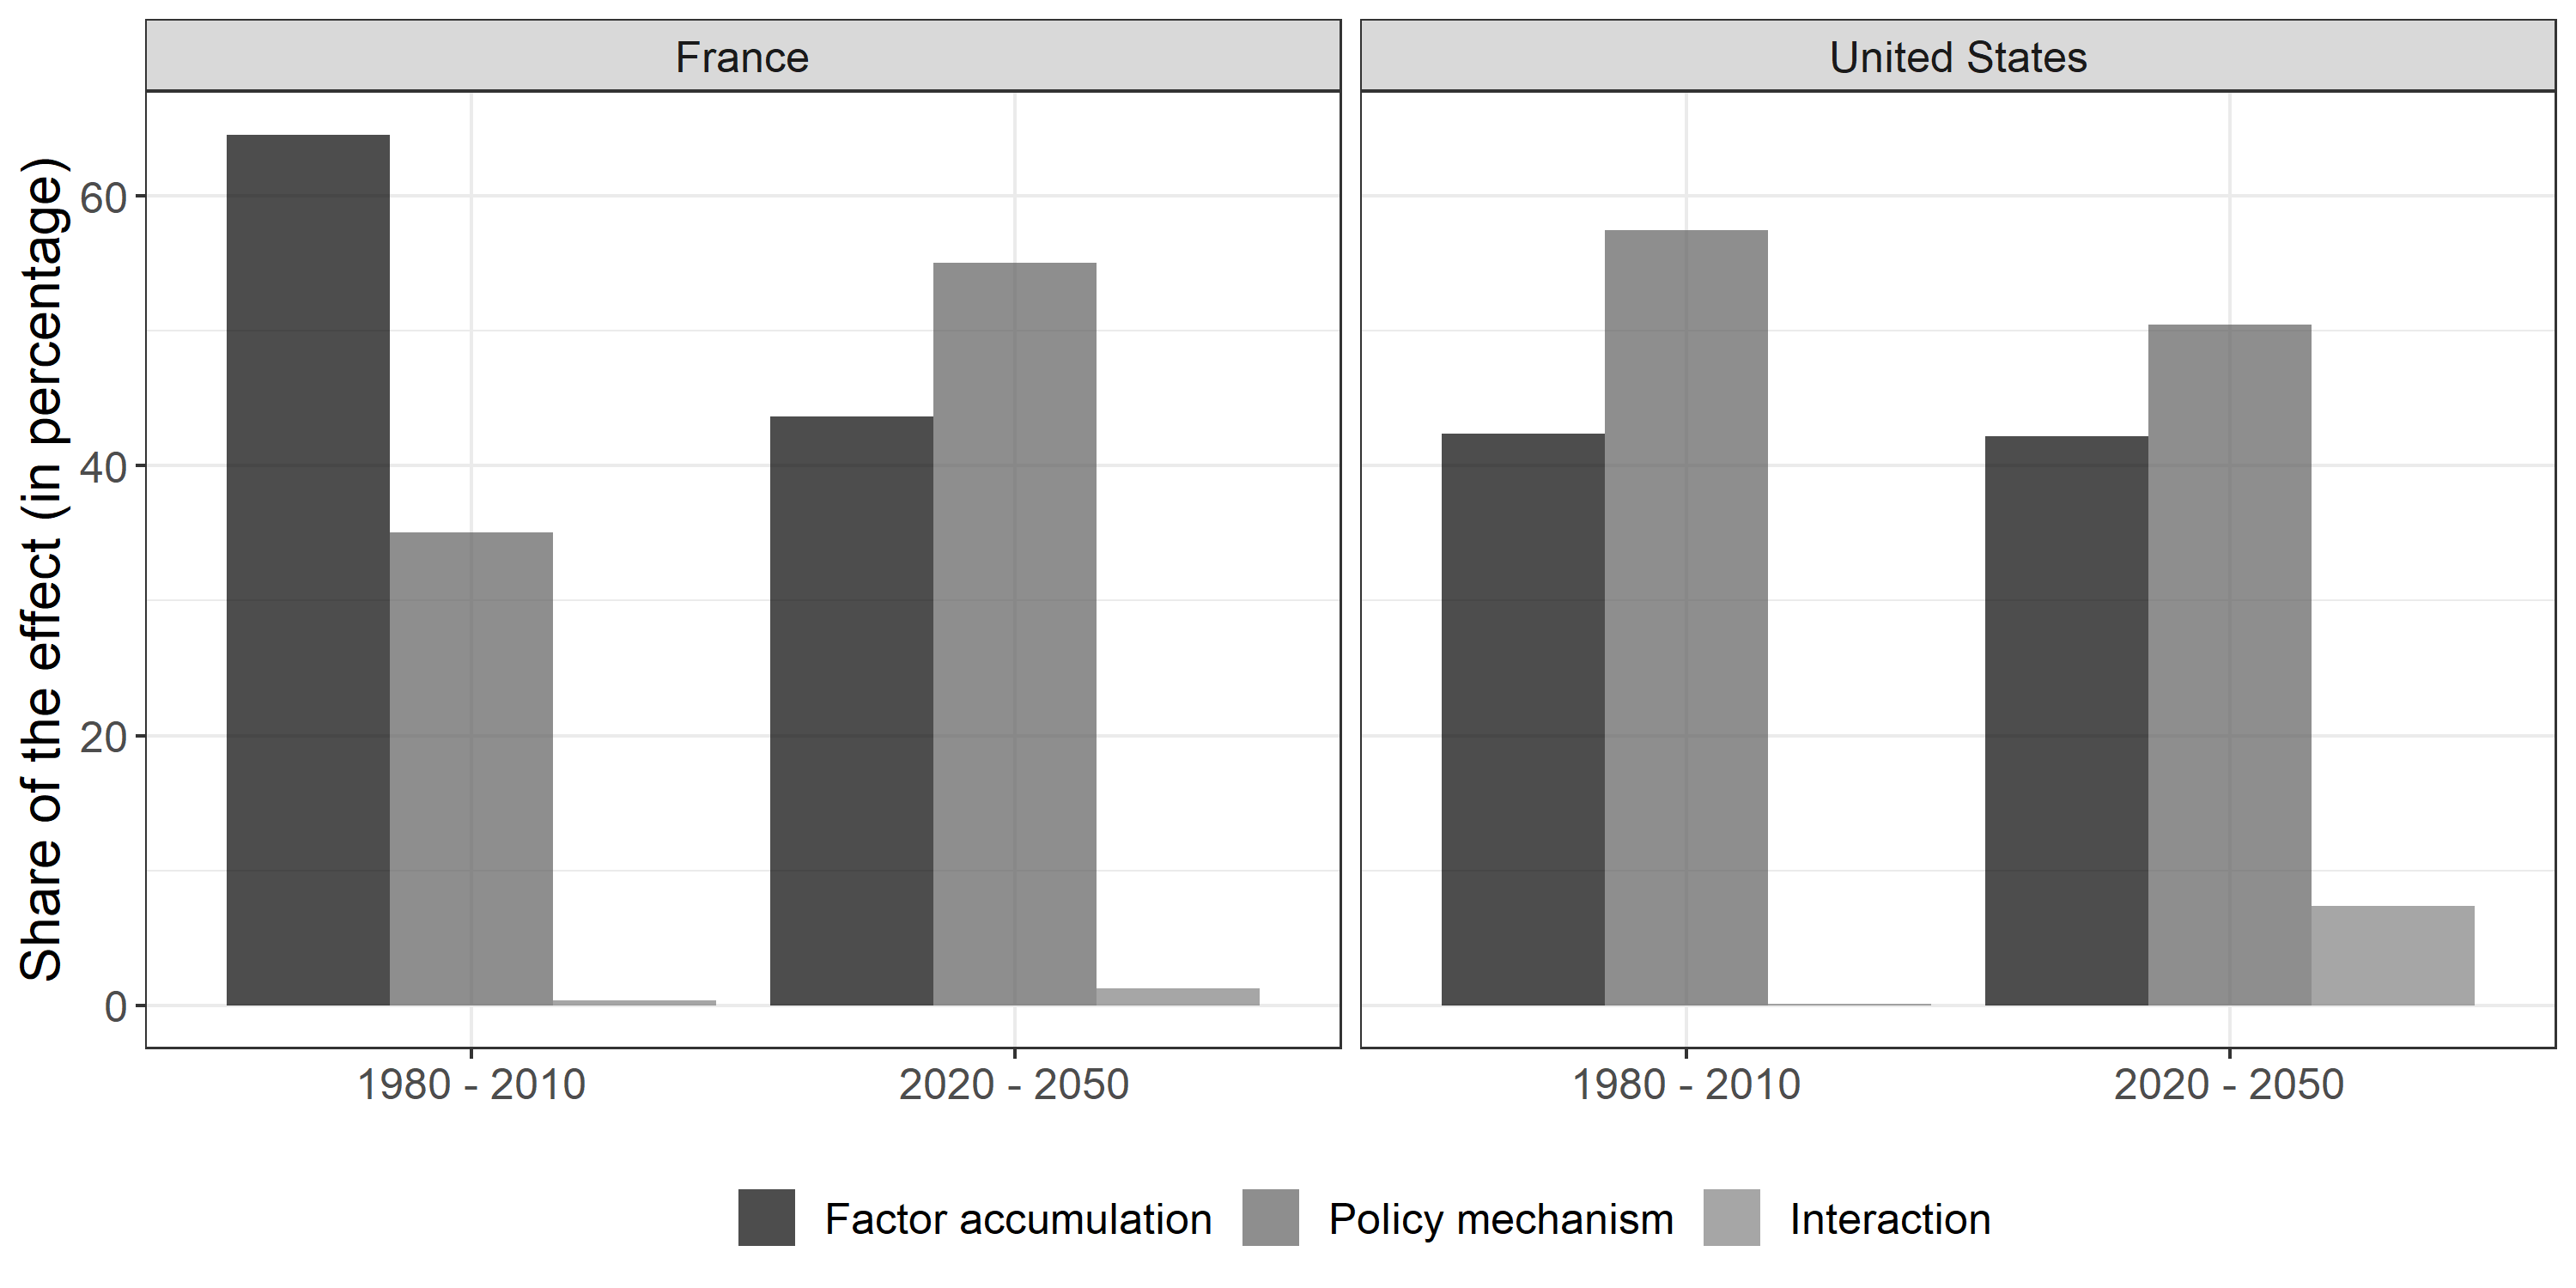
\includegraphics[width=1\linewidth]{chap1/graphic/quant-decomp-sum.png}
% 	\vspace{-3em}
% 	\justify\singlespacing\footnotesize\textit{Notes:} The figure shows the average percentage relative share of the channels of demographic changes on the labor share over the two periods of the boomers generation (young and old), for France and the United States. Data are from the counterfactual simulations of the model and summarize the results from figure \ref{chap1-fig:quant-decomp-channel}.
% \end{figure}
% Changes in the population growth rate and survival rate affect the labor share through two channels: the factor-accumulation effect and the policy-mechanism effect. When the boomers are young, the factor-accumulation effect dominates in France while the policy-mechanism effect prevails in the US. On average, the share explained by the policy-mechanism effect is about 35\% in France and 57.5\% in the US. Thereafter, between 2020 and 2050, the share of this latter effect rises by 20.8 pp. in France becoming the main channel, while it slightly decreases by 7 pp. in the US. These results suggest that the policy-mechanism effect accounts for more than half of the consequences of demographic dynamics on the labor share.

% Compare with SV2013
\citet{Schmidt2013Demographic} consider only the factor accumulation mechanism and show that this mechanism disappears in a small open economy because capital-per-worker and the wage rate are independent of domestic savings, so that labor share dynamics only reflect changes in net foreign assets.
% My approach
The major advantage of my approach is that the policy mechanism holds in a small open economy.
%
With capital mobility, \citet{Pica2010Capital} argues that competition to attract capital between countries leads to reduced labor market regulation and a lower labor share.
%
Nonetheless, he uses a Cobb-Douglas production function which cancels out the shift away from labor toward capital of firms that is allowed by the CES production function that I employ.
%
In terms of consequences for the labor share, the effect of capital markets integration that occurs through labor market deregulation in an open economy is equivalent to the response of the firms that substitute labor with capital to thwart workers' appropriation of the rents in a closed economy.

\subsection{Age-related conflict: who are the winners ?} \label{chap1-winners}

% So far
The results show that the labor share declines due to the size of the boomers' cohort in France and the US. First, when they are young they shape labor market institutions in their favor, raising wages but inciting firms to shift away from labor toward capital. Second, when they are old they have substantially increased the available capital in the economy through their savings, pushing firms to substitute even more. Although it may seem obvious that the boomers are the winners of the age-related conflict when they are old, the results raise the question of whether they were the losers when they were young because the labor share declined considerably over this period.

Although much emphasis is given to it in the policy debate, the labor share is a gross indicator of the income distribution that does not take into account redistribution. The net income ratio between young and old is more appropriate to determine the winners of the age-related conflict.\footnote{I do not consider the difference in lifetime utility between generations to assess who are the winners. The shape of the utility function does depend on the date at which a generation appears because the effective discount factor $\alpha p_{t+1}$ depends on life expectancy which varies across generations. Since two generations do not have the same baseline, then utility comparisons do not make much sense.}
Let $T$ be the per-capita redistribution from old to young that is the product between the old-age dependency ratio, i.e. $p_t/n_t$, and the difference between the after-tax and before-tax young-to-old income ratios, i.e. $Y_t^y/Y_t^o - \Theta_t$. Using equation \eqref{chap1-eq:after-tax-income-ratio},
\begin{equation*}
    T_t \equiv \frac{p_t}{n_t}\left(\frac{Y_t^y}{Y_t^o} - \Theta_t\right) =  \frac{p_t}{n_t}\left(\eta_t - \Theta_t\right).
\end{equation*}
Therefore, changes in per-capita redistribution reflect changes in the old-age dependency ratio, i.e. $p_t/n_t$, and in the aggregate redistribution, i.e. $\eta_t - \Theta_t$.

Figure \ref{chap1-fig:discuss-ratiopc} presents the per-capita redistribution from old to young in percentage deviation from its value in 1970.
\begin{figure}[!tb]
	\centering
	\caption{Per-capita redistribution dynamics} \label{chap1-fig:discuss-ratiopc}
	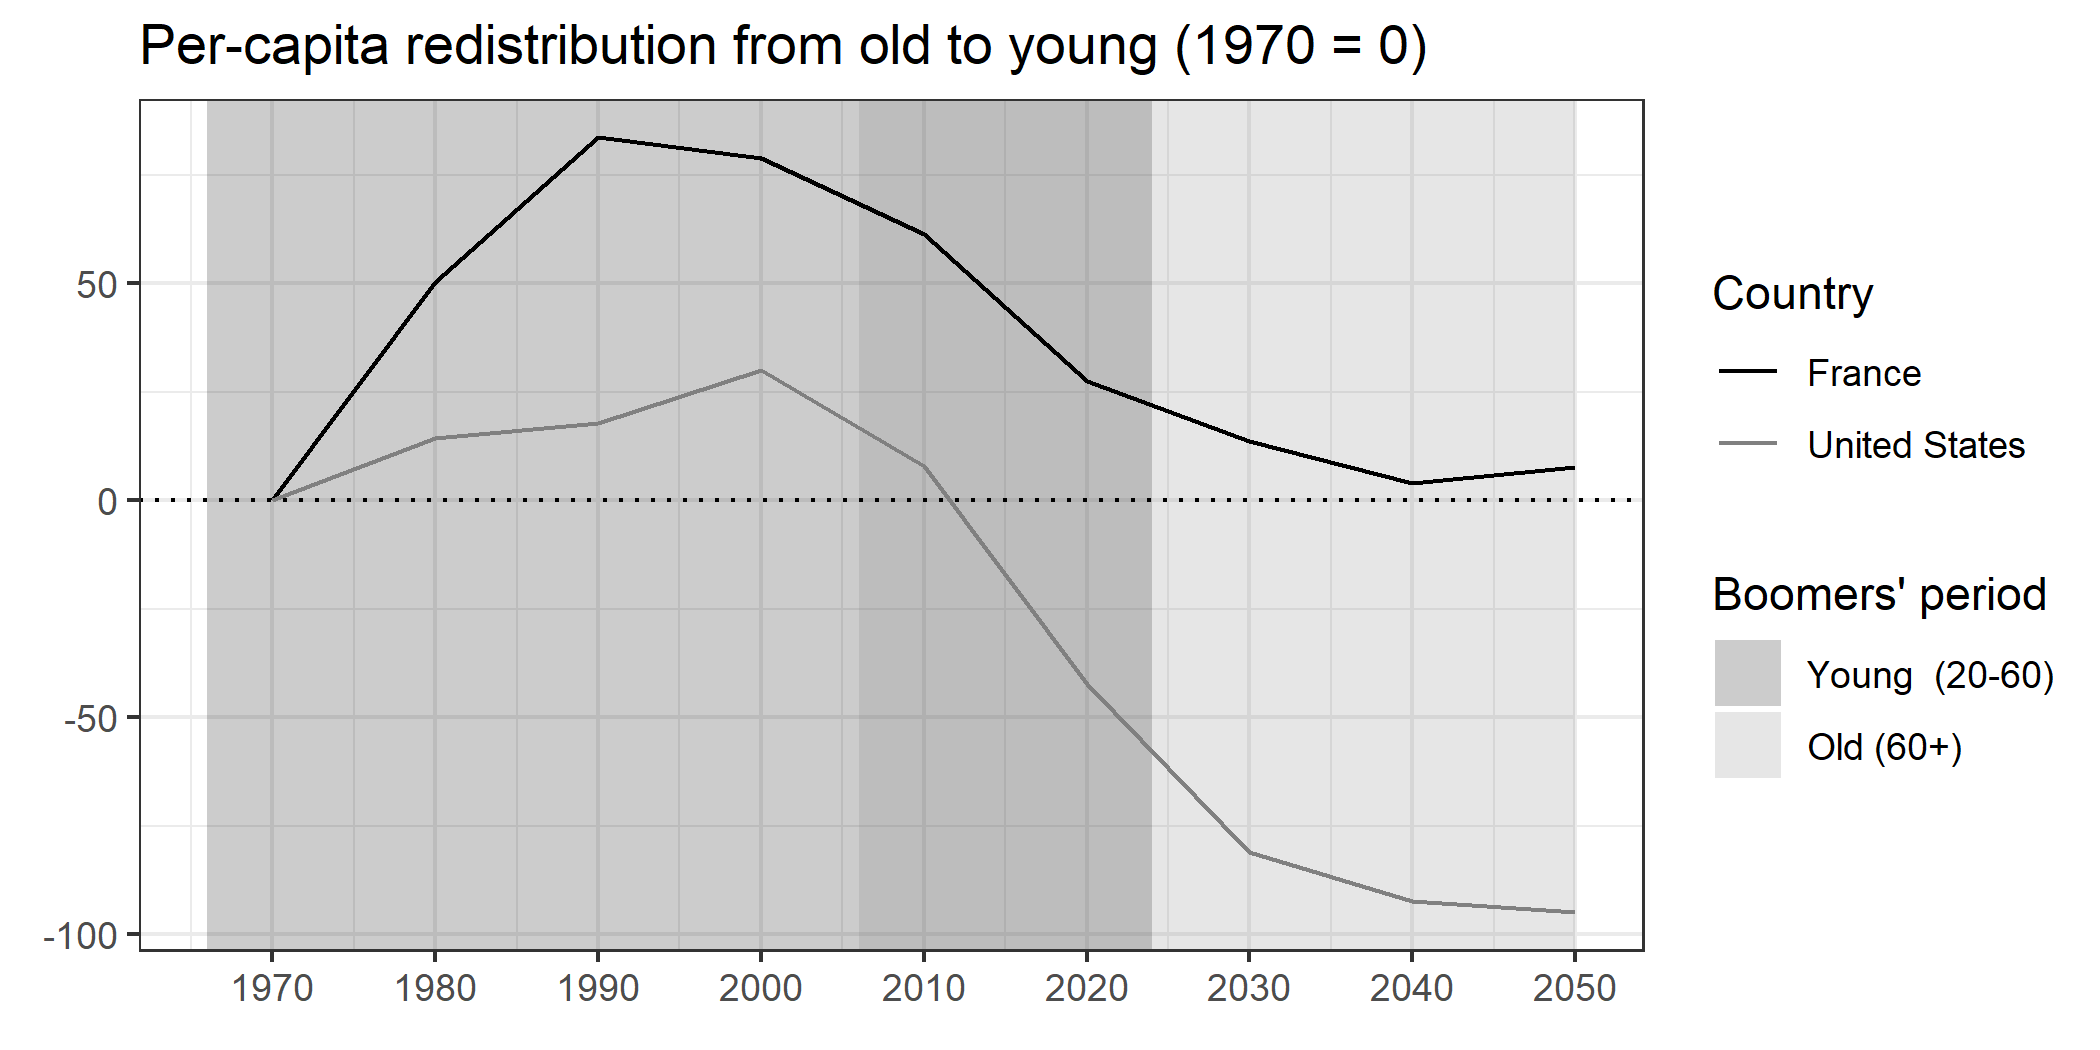
\includegraphics[width=1\linewidth]{chap1/graphic/discuss-ratiopc.png}
	\vspace{-3em}
	\justify\singlespacing\footnotesize\textit{Notes:} The figure shows the per-capita redistribution from old to young for France and the United States in percentage deviation since 1970. The black and grey lines represent, respectively, the France and the United States. The dotted line represents the 0-degree line. Rectangles define the periods when the boomers are young and old. Data are from the benchmark simulation of the model.
\end{figure}
When the boomers are young and enter the labor market (in 1970), they earn labor income until they start to retire in 2010. Over this period, the labor share declines and the per-capita redistribution from old to young increases in both countries. The young boomers are the winners of the age-related conflict over this period because they manage to recover their labor income losses by increasing redistribution due to their political weight. Once they retire and earn capital income, the labor share is rather stable, although the per-capita redistribution sharply declines. As a result, the boomers are also the winners of the age-related conflict when they are old because the level of redistribution from old to young declines. In the case of the US, the redistribution from old to young tends toward zero as the US economy is in full employment, hence, there is little need for unemployment benefits.\footnote{Note that the only source of heterogeneity is age, thus, there may be winners and losers within each cohort in presence of additional dimensions of heterogeneity, e.g. human capital.}
    
    \section{Conclusion} \label{chap1-conclusion}
    %% SUMMARY OF PAPER IDEAS AND MODEL
A vast literature emphasizes the role of biased technical change and institutions to explain the shift from labor toward capital and therefore the decline of the labor share observed in several countries over the past few decades. This paper focuses upstream of these determinants and highlights the role of demography as a force that shapes labor market institutions and hence the allocation of factor incomes. These institutions define the rules of the game for wage bargaining between firms and workers. When a particular generation, such as the boomers, can change institutions in its favor, then these rules also change, which affects the allocation of income between capital and labor. This mechanism accounts for the indirect \textit{policy-mechanism} effect of demographic changes on the labor share that results from the inter-generational conflict when choosing the public policy. Besides, the age structure of the population also has a direct \textit{factor-accumulation} effect that occurs through the labor supply and capital stock. Both effects combined help understand the role of the boomers' cohort in the decline of the labor share in France and the United States.

This paper shows to which extent we should take into account changes in institutions, that are endogenously determined by the age structure of the population, to understand macroeconomic dynamics in the long run. Decomposing the direct factor-accumulation effect and the indirect policy-mechanism effect, I find that the latter is as important as the former in explaining how demographic dynamics affect the labor share. Thus, omitting this indirect mechanism, and more broadly supposing that institutions do not change in the long run, leads to underestimating the role of demography on the factor income distribution. In this regard, my results provide a new conceptual framework to examine demographic dynamics and institutions in future work.

%% IMPLICATIONS IN TERMS OF POLICY DEBATE
These results have implications in terms of current policy debates. On the one hand, several high-income countries have experienced aging of their population which has led to a debate about optimal public policy. In this respect, my results shed light on the consequences of demographic changes on the allocation of income between capital and labor. On the other hand, developing countries are witnessing large demographic changes and may experience the arrival of a generation such as the boomers' cohort, which would change their institutions along with factor shares, and therefore, may have consequences on their development.
    
    %%% DO NOT CHANGE %%%
    \printbibliography[heading=subbibintoc]
    
    \clearpage
    \addsec{Appendices}
    \renewcommand{\thesubsection}{\thechapter.\Alph{subsection}}
    %%% DO NOT CHANGE %%%
    
    %%% APPENDICES
    
    \subsection{Probabilistic voting} \label{chap1-probabilistic}
    In order to determine their preferred public policy, households maximize their indirect utility function. Using the first order conditions from the household maximization problem in equations \eqref{chap1-eq:hhmaxc1}, \eqref{chap1-eq:hhmaxc2} and \eqref{chap1-eq:hhmaxs}, I obtain:
\begin{align}
	U_t^{y,i} &= \ln\left[\frac{1}{1+\alpha p_{t+1}}y_t^i\right]+ \alpha p_{t+1} U_{t+1}^{o,i}, \label{chap1-eq:utility_young} \\ 
	U_t^{o,i} &= \ln\left[\frac{\alpha p_t}{1+\alpha p_t}(1-\tau_t)y_{t-1}^i\hat{R}_t\right] + \beta \ln g_t, \label{chap1-eq:utility_old}
\end{align}
% Define indirect utilities
where $U_t^{y,i}$ is the indirect utility of a young household at time $t$ in employment status $i\in\{e, u\}$ and $U_t^{o,i}$ is the indirect utility of an old household at time $t$ who was in employment status $i$ in the previous period. 
% Depend on the first period income
Thus, indirect utilities depend on the first-period disposable income, $y^i_t$, and therefore the employment status.%
% PP prefs are functions of 1st period income
\footnote{Implicitly, public policy preferences are functions of the economic environment when the individuals are young. In line with the literature on preferences for redistribution, \citet{Giuliano2013Growing} show that individuals growing in recession tend to have greater preferences for redistribution; see also \citet{Alesina2011Preferences} for a general review of this literature. However, in this model, such a link is canceled by the logarithmic form of the utility function. For instance, the partial derivative of the indirect utility of the old with respect to either $\tau_t$ or $g_t$ does not contain the disposable income of the previous period $y_{t-1}^i$.}

% Timing => Young don't know their emp situation
The youth vote before their employment status is revealed.
% Vote based on expectation
They hence vote on the basis of their expected utility, corresponding to the weighted average of both indirect utilities, i.e. $\mathbb{E}({U}_t^y) = (1-u_t)U_t^{y,e} + u_t U_t^{y,u}$.
% Expected indirect utility
Therefore, the expected indirect utility of a young individual at time $t$ is
\begin{equation}
\begin{aligned}\label{chap1-eq:expected_utility_young}
	\mathbb{E}({U}_t^y) &= (1+\alpha p_{t+1})\left\{(1-u_t)\ln\left[\frac{(1-\tau_t) w_t}{1+\alpha p_{t+1}}\right] + u_t \ln\left[\frac{b_t}{1+\alpha p_{t+1}}\right]\right\} \\
	&+ \alpha p_{t+1} \bigg\{ \ln\left[\alpha p_{t+1} (1-\tau_{t+1}) \hat{R}_{t+1}\right] + \beta \ln g_{t+1} \bigg\},
\end{aligned}
\end{equation}
where $\mathbb{E}$ is the expectation operator. In contrast, the old have no uncertainty about the returns of their savings, thus, they vote on the basis of their indirect utility.

% Explain the proba voting setup
I consider a probabilistic voting setup.\footnote{The alternative would be a median voter setup. However, the median voter setup would create two extreme regimes with one of them being a gerontocracy. It would also generate large swings in public policy if the median-voter switches from young to old or vice versa. Under probabilistic voting, the equilibrium policy platform is a continuous function of the old-age dependency ratio.} With probabilistic voting, all agents vote for a policy platform $\psi_t = (\tau_t, b_t, g_t)$ represented by opportunistic candidates (or parties). Candidates try to maximize their probability of winning the election. They differ in their popularity and there is an idiosyncratic bias among voters for one candidate or the other. Candidates know about these biases. In equilibrium, all candidates choose the same policy platform $\psi_t^\star$ that maximizes the political objective function $W_t(\psi_t)$ defined below. See \citet{Lindbeck1987Balanced} for more details on the probabilistic-voting setup.

% Political objective function depends on pop share and omega
The political objective function depends on the share of each group of voters in the population and their respective sensitivity to policy changes $\omega^j$ with $j\in \{y,o\}$, where $\omega^j$ denotes the density parameter of the uniform distribution function that characterizes the ideology of the $j$ group. 
% Three groups of voters: YOUNG and OLD (emp and unemp 1st period)
There are two groups of voters: young and old households. Thus, I assume all elderly have the same sensitivity regardless of their employment situation when they were young.
% High omega => Spread ideology
The greater $\omega^j$, the more spread are the ideologies within the $j$ group. 
% Spread ideology => Easier for candidates to target
Hence, opportunistic candidates prefer targeting less ideological groups, i.e. large $\omega^j$, because they are easier to convince.
% EQ public policy
The equilibrium public policy $\psi_t^\star$ maximizes the following political objective function:
\begin{equation*}
	W_t(\psi_t) = \frac{N_t^y}{N_t} \omega^y \mathbb{E}\left[U_t^y(\psi_t)\right] + \frac{N_t^o}{N_t} \omega^o \Big\{ u_{t-1} U_t^{o,u}(\psi_t) + (1-u_{t-1}) U_t^{o,e}(\psi_t) \Big\},
\end{equation*}
subject to the government budget constraint from equation \eqref{chap1-eq:gov-budget}, where $\mathbb{E}\left[U_t^y(\psi_t)\right]$ and $U_t^{o,i}(\psi_t)$ are respectively defined by equations \eqref{chap1-eq:expected_utility_young} and \eqref{chap1-eq:utility_old}.

% Recall the no-coordination assumption
There is no coordination between voting and wage bargaining. Therefore, households only care about the direct effects of public policy on their utility. They do not consider the indirect effects operating through unemployment, wages, and the accumulation of capital. Let $\tilde{U}^i_t$ be the part of the utility which is directly affected by the public policy platform. From equation \eqref{chap1-eq:utility_old}, we have that $\tilde{U}_t^o = \tilde{U}_t^{o,u} = \tilde{U}_t^{o,e}$. 
% New political objective function
Hence, I rewrite the political objective function as
\begin{equation*}
	W_t(\psi_t) = \frac{N_t^y}{N_t} \omega^y \mathbb{E}\left[\tilde{U}_t^y(\psi_t)\right] + \frac{N_t^o}{N_t} \omega^o \tilde{U}_t^o(\psi_t) + \text{\textit{other~terms}}
\end{equation*}
where $\text{\textit{other~terms}}$ encompasses all the terms that are not directly affected by public policy.

% Define omega
Let $\omega$ be the \textit{relative ideological spread-out} of the youth with respect to the elderly. The relative ideological spread-out is characterized by the ratio of the sensitivities of voting behavior to policy changes for each group, i.e. $\omega \equiv \omega^y/\omega^o$. I assume this spread-out is constant over time.\footnote{This assumption can be interpreted in two ways: either both relative ideological spread-outs are time invariant or they vary in same proportions. It would be interesting to consider these spread-outs as endogenous or to make them cohort-specific. This goes beyond the scope of this paper.} Using equations \eqref{chap1-eq:utility_old} and \eqref{chap1-eq:expected_utility_young}, I rewrite the maximization program that characterizes the public policy equilibrium as 
\begin{align*}
	\max_{\tau_t, b_t, g_t} W_t(\tau_t, b_t, g_t) &= \eta_t \bigg[ (1-u_t)\ln(1-\tau_t) + u_t \ln b_t\bigg] + \ln(1-\tau_t) + \beta \ln(g_t) \\
	&+ \text{\textit{other~terms}}
\end{align*}
subject to the government budget constraint from equation \eqref{chap1-eq:gov-budget}, where 
\begin{equation*}
	\eta_t = \frac{n_t}{p_t}\omega(1+\alpha p_{t+1})
\end{equation*}
is the \textit{political weight of the young}.
    \clearpage
    \subsection{Methodology for counterfactual simulations}\label{chap1-countermetho}
    In this appendix, I provide details on the methodology for the simulations and decompositions in section \ref{chap1-counterfactual}. The benchmark simulation is the one obtained in section \ref{chap1-model_pred}. In what follows, a variable with a prime denotes the new value of this variable that is used in the counterfactual simulation. 

\textbf{Factor-accumulation counterfactual simulation.} I neutralize the factor accumulation effect by setting the rate of population growth and the survival rate at their levels in 1970, i.e. $n^\prime_t = n_{1970}$ and $p^\prime_t = p_{1970}$.
The expected survival rate $p_{t+1}$ of one generation is the survival rate $p_t$ once this generation becomes old, therefore it implies that $p_{t+1}^\prime = p_t^\prime = p_{1970}$.
Thus, the numbers of young and old households in the first period of each sequence, i.e. from 1970 to 2000, are recalculated to be consistent, such that
\begin{equation*}
    N_t^{y\prime} = \frac{n^\prime_t}{n_t} \times N_t^y  ~\text{ and }~    N_t^{o\prime} = \frac{p^\prime_t}{p_t} \times N_t^o,
\end{equation*}
This change affects demographic dynamics, which are therefore recalculated for the second and third periods of each sequence, i.e. from 2010 to 2080, such that
\begin{equation*}
    N_t^{y\prime} = n^\prime_t N_{t-1}^{y\prime} ~\text{ and }~    N_t^{o\prime} = p_t N_{t-1}^{y\prime}.
\end{equation*}
The capital stock in the first period of each sequence, i.e. from 1970 to 2000, is recalculated such that
\begin{equation*}
    K_t^\prime = \frac{1+\alpha p_t}{\alpha p_t}\frac{\alpha p_t^\prime}{1+\alpha p_t^\prime} K_t.
\end{equation*}
The initial capital stocks are recalculated because setting constant the survival rate implies changes in the saving rate as
\begin{equation*}
    K_t \equiv S_{t-1} = \frac{\alpha p_t}{1+\alpha p_t} Y^y_{t-1},
\end{equation*}
where $Y^y_{t-1}$ is the aggregate net income of young households.
Thus, not taking into account the change in the saving rate would bias the interpretation of the effect of survival rate dynamics by leaving behind part of the effect that occurs through capital accumulation.

\textbf{Policy-mechanism counterfactual simulation.} I neutralize the policy-mechanism effect by setting only the political weight of the young at its level in 1970, i.e. $\eta_t^\prime = \eta_{1970}$. All other demographic variables remain identical to the benchmark simulation.

\textbf{Baseline counterfactual simulation.} I neutralize both effects, therefore, I set $n^\prime_t = n_{1970}$, $p^\prime_t = p^\prime_{t+1} = p_{1970}$. This simulation is the combination of the two previous ones. As before, the number of young and old households along with the capital stock at first period of each sequence, i.e. from 1970 to 2000, are recalculated. These changes affect the dynamics of young and old households which are therefore recalculated for the second and third periods of each sequence, i.e. from 2010 to 2080.
For every year, the political weight of the young remains at its level in 1970, i.e. $\eta^\prime_t = \eta_{1970}$

\textbf{Factor accumulation versus policy mechanism.} 

Figure \ref{chap1-fig:quant-counter-channel} presents the labor share from the four counterfactual simulations, as detailed above.
\begin{figure}[!htb]
	\centering
	\caption{Counterfactual simulations of the channels of demographic changes.} \label{chap1-fig:quant-counter-channel}
	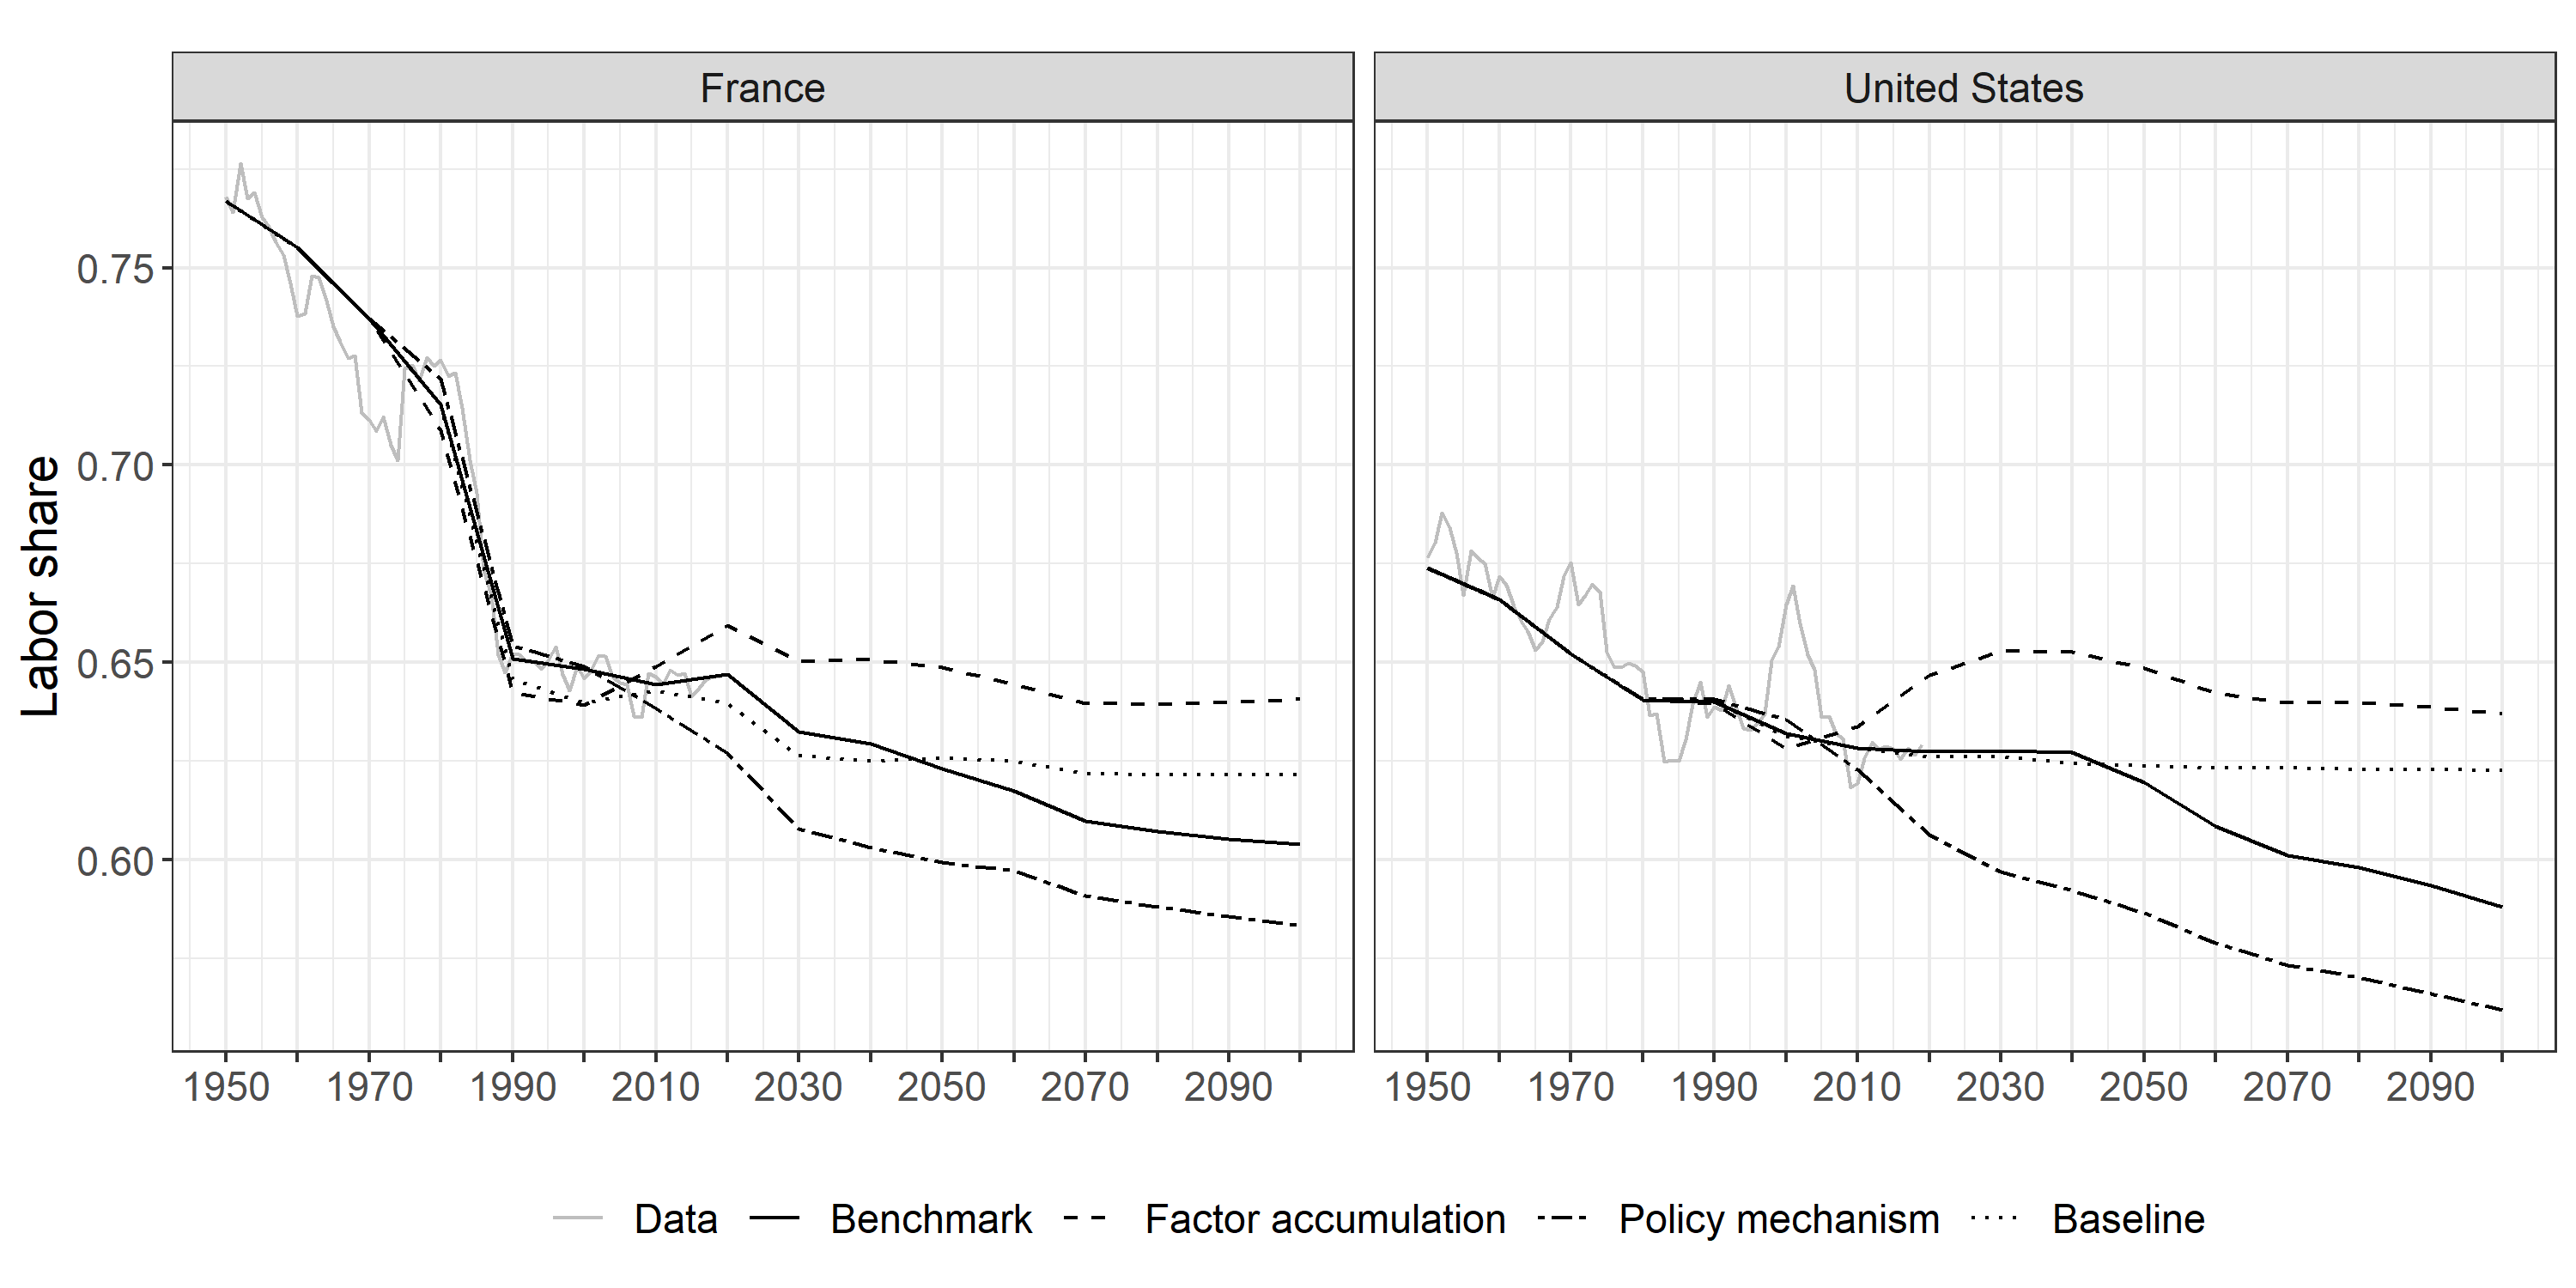
\includegraphics[width=1\linewidth]{chap1/graphic/quant-counter-channel.png}
	\vspace{-3em}
	\justify\singlespacing\footnotesize\textit{Notes:} The figure shows the counterfactual simulations of the channels of demographic changes on the labor share. 
	Labor share data are from the \href{https://www.rug.nl/ggdc/productivity/pwt/}{Penn World Table 9.1} with self-employed income as labor compensation.
	The benchmark labor share corresponds to the benchmark predictions of the model. The factor-accumulation simulation refers to the labor share of the counterfactual simulation in which the factor-accumulation channel is neutralized. The policy-mechanism simulation refers to the labor share of the counterfactual simulation in which the policy-mechanism channel is neutralized. The baseline labor share corresponds to the predictions when both channels are neutralized.
\end{figure}
From this figure, I derive the decomposition of the channels of demographic changes, see figure \ref{chap1-fig:quant-decomp-channel}.

\end{refsection}

	\chapter{Spreading the polarization disease: from the labor market to social mobility}\label{chap2}
	\textit{This chapter is based on a joint research with Cecilia García-Peñalosa (Aix-Marseille University) and Tanguy van Ypersele (Aix-Marseille University).}\\
\vspace{1em}\\
\noindent \textbf{Abstract}: The increase in employment polarization observed in a number of high-income economies has coincided with a reduction in inter-generational mobility. This paper uses data for two British cohorts that entered the labour market at two points in time that differed considerably in terms of the structure of employment to re-examine the drivers of mobility. 
We differ from the existing literature in two aspects. First, we focus on employment categories rather than income, thus obtaining dynamics that can be understood in terms of changes in the structure of employment. Second, we argue that understanding inter-generational dynamics requires considering how individuals move from their entry jobs into other employment categories, i.e. understanding intra-generational mobility. 
The data indicate that occupational changes over the individual’s career are an important source of mobility, with large shares of those in low-paying (respectively, middling) occupations moving into middling (resp. high-paying) ones. When we compare the two cohorts we find that these two sources of mobility have declined for the younger cohort and that, whatever the initial occupation, parental income has become more important in leading to occupational upgrading. 
Moreover, the impact of parental income increased the most in the regions where the share of middling employment fell the most, suggesting that increased employment polarization may be one of the factors behind the observed decline in mobility.\\
\vspace{1em}\\
\noindent\textbf{Keywords:} Inter-generational mobility, Job polarization.\\
\noindent\textbf{JEL Codes:} J62, J21, J24.

\clearpage
\chaptertoc{}

\pagebreak

\begin{refsection}
    
    \section{Introduction}\label{chap2-introduction}
    A recent literature has documented a decline in income and social mobility in the last decades of the 20th century that has strengthened the link between individuals' origins and their socio-economic outcomes; see, for example, \citet{Blanden2007Accounting} for the UK and \citet{Chetty2020Race} for the US.
%Understanding what has driven such a decline is therefore crucial to policy makers in order to reassert equality of opportunity. 
Existing work has proposed several explanations for the reduction in mobility, focusing, for example, on educational investments, non-cognitive skills, or the impact of geographical location, yet little attention has been paid to the role of the structure of employment. This is surprising given that the decrease in mobility has taken place roughly at the same time as labour markets in high-income economies witnessed an increase in employment polarization. Since the 1980s, the share in total employment of low- and high-paying occupations has increased at the expense of that of middling occupations,\footnote{See, for example, \citet{Autor2003Skill}, \citet{Autor2006Polarization}, \citet{Goos2007Lousy}, \citet{Dustmann2009Revisiting}, \citet{Goos2009Job}, and \citet{Cortes2016Middle} on the extent of polarization.} raising the question of whether individuals from less well-off backgrounds can still climb the social ladder as the middle rungs become scarce. 

This paper bridges the gap between the literature on social mobility and that on employment polarization. To do so, we depart from existing work in two respects. First, mobility is not defined in terms of income, as the literature tends to do;\footnote{While economists have tended to examine income mobility (e.g. \citealt{Blanden2007Accounting}, \citealt{Blanden2013Intergenerational}, \citealt{Chetty2014Land}), the literature on social mobility focuses on the analysis of socio-economic class. See \citet{Erikson1992Constant}, as well as \citet{Chan2007Class} and \citet{Erikson2010Social} for a discussion on social class and inter-generational mobility in the United-Kingdom.} rather we focus on occupations and define occupational categories in line with the employment polarization literature (see, for example, \citealt{Goos2014Explaining}). This allows us to identify whether the increased impact of parental income is being driven by how family background affects occupational outcomes. Second, while existing work on inter-generational mobility focuses on the correlation between parental characteristics and the outcomes of mature children, we argue that it is important to disentangle changes in mobility that are due to the \textit{intra-generational} component ---defined as the transition between the entry job and the job when mature--- from those due to the initial job that individuals hold. This change of emphasis allows us to examine whether the impact of parental income is correlated to changes in the structure of employment, thus raising the question of whether polarization has been one of the causes of the decline in mobility. 

We start our analysis by developing a simple model with two employment periods and three occupations, in which individuals differ both in parental income and innate ability. The latter is not initially observable by firms but may be observed at the end of the first period of employment. Crucially, we argue that different occupations have different informational contents. In particular, we suppose that while high-paying and middling jobs reveal the ability of the individual, low-paying jobs do not. 

We consider, for simplicity, only two levels of parental income such that when individuals are young those with low-parental income are initially randomly allocated to either low-paying or middling jobs, and those with high parental income to high-paying or middling jobs. In the second period, ability is revealed making those from poor households and with high ability switch occupations with those from rich households and with low ability. In this context, the availability of middling jobs is the key element determining the extent of mobility. With only a small number of middling jobs, the majority of those from low-income backgrounds will start their careers in low-paying jobs. Because only the few that are initially in middling jobs can reveal that they are of high ability, only a few individuals with low-income parents will be promoted into high-paying occupations and as a consequence few of those who started in high-paying occupations will be demoted. The result will be a lower degree of mobility than when middling jobs are plentiful.

The core of our analysis is an empirical assessment of occupational mobility which uses data from two mature British cohorts, the National Child Development Study (NCDS58) and the British Cohort Study (BCS70). The surveys cover individuals born in, respectively, 1958 and 1970 for whom we have full activity histories along with parental income. These data have been widely used to address the extent of mobility in the UK and existing work indicates that parent-child income mobility has declined for the younger cohort as compared to the older one.\footnote{See for example \citet{Blanden2007Accounting}, \citet{Nicoletti2007Intergenerational}, and \citet{Blanden2013Intergenerational}, as well as the work by sociologists such as \citet{Goldthorpe2007Intergenerational} and \citet{Erikson2010Social}.} Because we are interested in the structure of employment, we define four occupational categories, low-paying, middling and high-paying jobs, in line with the employment polarization literature, as well as a category including those out-of-work. The data also allows us to consider occupational outcomes both at the start of the individual's career\footnote{The ages at which interviews take place for the two cohorts are not identical. Both were interviewed at 42 years of age but differ in the ages of the earlier interviews, with those born in 1958 (resp. 1970) having an interview at age 23 (resp. 26). We use these ages to measure early-career occupations.} as well as when workers are mature, i.e. at age 42, and hence to consider occupations at different stages of the work-life.

Existing work on mobility has taken two approaches, either focusing on the correlation between the child's income or social status at around 40-years of age and that of the parent or examining lifetime dynamics independently of parental background.\footnote{See \citet{Jantti2015Income} for a review.} Our empirical framework aims to disentangle changes in social mobility that are due to the \textit{intra-generational} component ---defined as the transition between the entry job and the job when mature--- from those due to the \textit{inter-generational} component. We proceed in two steps, estimating first the impact of parental income on the child's first-period occupation and then the effect of first-period occupation on the occupation at age 42, as well as whether there is any remaining direct effect of parental income. We can hence ask whether the decline in mobility observed over the period is due to a greater impact of parental background on entry jobs or if the change has occurred mainly through differences in transition probabilities over the child's lifetime. 

Our focus is the comparison between the results for the 1958 cohort and those for the 1970 cohort. Our data indicate that the polarization that has been observed at the aggregate level also appears when we consider the employment structure for each cohort, indicating that those born in 1958 entered the labour market when middling jobs were plentiful, while those born in 1970 faced greater employment polarization. Moreover, the change in the structure of employment has been particularly marked regarding first-period occupations. To further understand the relationship between polarization and mobility, we measure both at the regional level. We consider differences in the impact of parental income on occupational outcomes (i.e. the degree of \emph{immobility}) across large regions, and construct for each region a measure of employment polarization for each cohort using data from the Labour Force Survey so as to compute the change in the extent of polarization faced by the two cohorts. This allows us to correlate the change in \emph{immobility} and the change in the share of middling employment at the regional level in order to ask whether these two variables have moved together. 

Our analysis provides three main results. The first concerns the fact that intra-generational mobility is an essential aspect of the observed correlation between parent and child outcomes. We find that for both cohorts individuals face a large likelihood of changing occupational category over their career. Notably, around 23\% and 30\%, respectively, of those initially in low-paying and middling occupations are in high-paying occupations when they are 42. In fact, for those two groups, less than half of those who were in each occupational category when young are in the same one as mature workers, with both the probabilities of moving upwards and downwards being large. Persistence is much higher for those starting in the best-paid jobs, but nevertheless, a third of them experience downwards mobility. Our results hence imply that it is important to understand career dynamics in order to explain the transmission of economic outcomes across generations.

Second, we find that the increased impact of family background on children's incomes identified in previous work also appears when we focus on occupations.\footnote{A few studies have considered occupational mobility, notably \citet{Long2013Intergenerational} who take a three-generation perspective, and \citet{Bell2018Land} who use recent British data. The occupational categories used are however not the same as those found in the employment polarization literature. For example,  \citet{Long2013Intergenerational} build four categories: white-collar, farmer, skilled and semi-skilled, and unskilled. \citet{Bell2018Land} use narrow occupational categories that they rank by median wages.} Moreover, the reduction in mobility is apparent at all the stages that determine an individual’s occupation when mature, as both the effect of parental income on first-period occupation and that on the job when mature controlling for initial occupation have become stronger for the younger cohort. These results raise the question of what are the implications of the disappearance of middling jobs for mobility. On the one hand, fewer individuals have access to those jobs when young, and those who do tend to come from better-off backgrounds; on the other, whether those in middling jobs move to high-paying occupations is more dependent on parental income for the younger than for the older cohort. The overall outcome are increased differences in intra-generational mobility according to family background. For those at the top of the parental-income distribution, upwards mobility during the working life has risen by about 5 percentage points, both for those starting in low-paid or middling jobs; in contrast it has declined by around 8 percentage points for those from less well-off families, irrespective of what job they initially held. That is, we observe that the possibility of career progression has become more dependent on parental background.

Lastly, when we exploit the regional dimension of our data we find a correlation between mobility and polarization which appears both over time and in the cross-section. At the individual level, our results indicate that the effect of parental income on occupational outcomes is stronger for individuals that---when young--- lived in areas with greater job polarization, indicating that a possible reason for the observed decline in mobility across the two cohorts is the disappearance of middling jobs.  
We then consider differences in \emph{immobility} across large regions and find that regions that have experienced a greater decline in the share of middling jobs are also those in which the impact of parental income has increased the most. These correlations are indicative that the disappearance of middling jobs may be one of the reasons behind the observed decline in mobility.

Our work is related to three strands of literature. 
First, it contributes to the literature on the determinants of inter-generational mobility which has extensively documented the parent-child dynamics in income and social class.\footnote{See, for example, \citet{Nicoletti2007Intergenerational}, \citet{Kopczuk2010Earnings}, \citet{Blanden2013Intergenerational}, \citet{Long2013Intergenerational}, and  \citet{Chetty2014United}, \citet{Chetty2017Fading} for work on inter-generational income mobility and \citet{Erikson1992Constant}, \citet{Chan2007Class}, \citet{Goldthorpe2007Intergenerational}, and \citet{Erikson2010Social} on social class.} Much of the focus has been on how individual characteristics affect income dynamics across generations, notably education,  non-cognitive skills and personality traits, and the quality of the neighborhood.\footnote{See \citealt{Bjorklund2012Important}, \citealt{Blanden2014Education}, \citealt{Blanden2016Educational}, \citealt{Crawford2016Higher}, and \citealt{Neidhofer2018Educational} on education, \citealt{Chetty2020Race} ) on race, and \citealt{Heckman2006Effects}, \citealt{Blanden2007Accounting}, \citealt{Heckman2013Understanding}, and \citealt{Chetty2014Land}) on other childhood outcomes.} Yet little attention has been paid to the importance of early labour market experiences. This paper hence provides a bridge between the literatures on \textit{inter-generational} and \textit{intra-generational} mobility by focusing on access to jobs at the beginning of the career and the subsequent career dynamics, and shows that understanding \textit{intra-generational} mobility is essential to understand an individual's outcome when mature. 

Our paper is particularly close to the recent literature that has identified a reduction in income mobility and an increased role of parental background, notably in the US and the UK. Part of this effect seems to operate through education. For example, for the UK, \citet{Blanden2004Family} and \citet{Gregg2010Family} find a rising impact of parental income on children's educational attainment. More recent work, such as \citealt{Chetty2014United} has shown the importance of the location where the individual grew up for inter-generational income dynamics. Our contribution lies in showing that the increased importance of parental income also appears when we focus on occupational categories, and that this operates in part through a stronger influence of family background on the probabilities of moving from one occupation to another.

Lastly, our paper adds to our understanding of the consequences of employment polarization. Much of this literature has used search models and taken a macroeconomic approach to understand the causes and consequences of polarization. The role of routine-biased technological change has been at the center of the debate. Starting with \citet{Autor2003Skill}, these analyses maintain that advances in information and communication technology affected the structure of employment because the tasks that computers are good at performing are concentrated around a set of middle skills that have a considerable ``routine'' component.\footnote{See also \citet{Goos2014Explaining}, \citet{Caines2017Complex}, \citet{Lordan2018People}, and \citet{Acemoglu2020Robots}, i.a..} The tasks approach which assigns skills to tasks based upon comparative advantage has been fruitful in creating a framework that allows us to understand the allocation of labour both within and across countries, and its implications for the structure of employment and wages. Our paper departs from this literature by proposing a model based on the idea that tasks also differ in the possibilities they give individuals to transmit information to firms about their (initially) unobservable ability. As a result, different occupations will have a different potential to reveal individuals' skills, with important implications for occupational dynamics.

Concerning the consequences of polarization, economists have mainly focused on the distribution of earnings,\footnote{This literature has grown rapidly over the past decade. See, amongst others, \citet{Autor2013Growth}, \citet{Beaudry2016Great}, \citet{Caines2017Complex}, \citet{Ross2017Routine}, \citet{Barany2018Job}. and \citet{Longmuir2020Routinization}.} although there is some work on its impact on educational attainment or the labour supply  (\citealt{Spitz-Oener2006Technical}; \citealt{Verdugo2020Labour}). The task approach introduced by \citet{Autor2003Skill} implies that biased technological change results in both the polarization of employment and a change in wages, and much work has been devoted to trying to understand to what extent polarization has driven observed increases in earnings inequality.\footnote{The widespread view is that indeed the changing structure of employment has resulted in increased earnings dispersion; see the overview in \citet{Acemoglu2011Skills}. Some authors nevertheless disagree; see \citet{Hunt2019Employment}.} Surprisingly, the question of whether employment polarization affects mobility has been largely ignored. To our knowledge, the only exception is \citet{Hennig2021Labor}, who examines the relationship between the structure of employment and income mobility. He builds a model in which the disappearance of routine jobs results in a polarization of education and lower inter-generational mobility, predictions that are shown to be consistent with patterns of inter-generational income mobility in the US. In his framework, the occupation of mature workers is determined exclusively by their educational choice; we hence complement his work by adding an analysis of job-to-job transitions. We show that these transitions are essential to understand mobility and, when we turn to regional data, that they are correlated with the increase in polarization across cohorts. 

The paper is organised as follows. We start by presenting a simple model of the effect of employment polarization on occupational mobility. Section \ref{chap2-data} presents the cohort data and describes the structure of employment for the two cohorts along with their occupational dynamics. We discuss our empirical specification in Section \ref{chap2-specification}, which distinguishes between the effect of parental income on initial occupations and on the transition across occupations during the individual's worklife. Section \ref{chap2-mobility} focuses on the patterns of occupational mobility, examining the changes that have occurred across the two cohorts. The final step in our analysis, provided in Section \ref{chap2-regional}, is to estimate mobility at the regional level and provide evidence on the correlation across regions between the extent of job polarization and changes in mobility. Section \ref{chap2-conclusion} concludes.

    
    \section{Theoretical framework} \label{chap2-model}
    We start by developing a simple theoretical setup that relates polarization to mobility. We consider three types of jobs $j = \{1,2,3\}$, which can be interpreted, respectively, as low-paying, middling and high-paying jobs. Parents transfer human capital to their children and the latter’s productivity, and hence allocation to jobs, is determined both by transmitted human capital and innate (and initially unobservable) ability. Children’s entry jobs will be determined by parental background, but as their ability is revealed, they may move up or down the job ladder. The aim of the model is to illustrate how mobility changes as the share of middling jobs falls.

\subsection{Workers' skills and family background} \label{chap2-model-workers}

We suppose that there are two types of parental background, which we denote by low-income ($L$) and high-income ($H$). The difference between the two groups can encompass income or human capital; what is important for our purposes is that children of $H$-parents have more initial human capital than those of $L$-parents, whether through direct transmission or the possibility of accessing better schools or more years of education. We denote by $z_i$ the share of parents with background $i = \{L,H\}$, with $z_H + z_L = 1$.

Individuals also differ in their innate ability, which will be high with probability $\pi$ and low otherwise, and is assumed not to depend on parental type. Ability is assumed to have no effect on first-period productivity but will affect that in the second period. Ability is potentially observable---by the individual and by the firm---at the end of the first period. We suppose that the individual can always observe her ability but has no way of truthfully revealing it to the firm. Our key assumption is that whether ability is observed by the firm depends on the type of job that the individual performed in the first period. In particular, we suppose that ability is observed by the firm if the individual worked in middling or high-paying occupations but not if she worked in a low-paying occupation. \footnote{The underlying idea is that the simple tasks performed in this kind of occupation make it impossible to infer how capable the individual will be in other types of occupations. Alternatively, we could have considered the possibility that certain jobs allow for the accumulation of human capital which is complementary with ability, while others do not.} 

Assuming that parental type perfectly determines the initial skills of the child, the human capital of an individual in the first period is simply $h_L$ or $h_H$ for those with low- and high-income parents, respectively, and there will be a share $z_L$  and $z_H$ of young individuals of each type. Second period productivity is supposed to depend on both parental background and ability. We denote by $\underline{h}_i$, respectively $\overline{h}_i$, the second-period human capital of an individual of type $i$ that is of low, respectively high, ability. The resulting productivities are ranked as follows: $\underline{h}_L < \underline{h}_H < \overline{h}_L < \overline{h}_H$, implying that while parental background matters, high ability individuals are always more productive than those with low ability irrespective of family background. 

\subsection{The structure of employment} \label{chap2-model-structure}

Denote the share of low-paying jobs by $q_1$, the share of middling jobs by $q_2$, and the share of high-paying jobs by $q_3$. . Since the wage of high-paying (resp. middling) jobs is greater than that of middling (resp. low-paying) jobs, employers fill jobs of each type with the most skilled worker available. 
The model can present various allocations of individuals across occupations depending on parameter values. We focus in a particular case which illustrates the mechanism we have in mind. To do so we make two assumption on parameter values:
\begin{assumption}\label{chap2-ass:threshold-skill-p1}
We suppose that the share of low-income parents, $z_L$, satisfies $1-q_3 > z_L > q_1$.
\end{assumption}
Assumption \ref{chap2-ass:threshold-skill-p1} ensures that in the first period some individuals from both high- and low-income parental backgrounds are in occupation 2.
\begin{assumption}\label{chap2-ass:threshold-skill-p2}
We suppose that the share of high-ability individuals, $\pi$, satisfies $ \frac{q_3}{1-q_1} > \pi > 1- \frac{q_1}{z_L-q_1} $.
\end{assumption}
Assumption \ref{chap2-ass:threshold-skill-p2} characterizes the second period allocations. It ensures that (i) not all low-ability individuals from low-income households work in occupation 1 and (ii) some low-ability individuals from high-income household work in occupation 3. 

\subsection{The allocation of labour} \label{chap2-model-allocation}

Employers fill jobs sequentially according to the worker's human capital. Table \ref{chap2-tab:init-prb-p1} summarizes, under Assumption \ref{chap2-ass:threshold-skill-p1}, the distributions of jobs in the first period. The distribution of jobs and skills in the population are such that only workers with low-income (resp. high-income) parents are initially in low-paid (resp. high-paid) occupations, while both types of individuals are found in middling jobs in the first period.

\begin{table}[!htb]
    \centering
    \caption{First-period allocation of labour}
    \label{chap2-tab:init-prb-p1}
    \begin{threeparttable}
        \setlength{\tabcolsep}{12pt}
        \setlength{\extrarowheight}{6pt}
        \begin{tabular}{r|c|c}
            & $L$ & $H$ \\
            \midrule
            Low-paying & $q_1$ & $0$ \\
            Middling & $z_L - q_1$ & $z_H - q_3$ \\
            High-paying & $0$ & $q_3$
        \end{tabular}
    \end{threeparttable}
\end{table}

In the second period, the allocation of individuals across jobs depends on three factors: parental background, ability, and the occupation in which the individual worked in the first period. Notably, the latter matters because of our assumption that ability is not revealed for those in low-paying occupations. 

Consider those who start in low-paying occupations and for whom ability is not revealed. Firms will attribute them their expected productivity which is given by $\widehat{h}_L\equiv (1-\pi )\underline{h}_{L}+\pi \overline{h}_{L}$. We assume this expression to satisfy $ \underline{h}_{L} < \widehat{h}_L < \underline{h}_{H} $. That is, those who have worked in low-paying occupations have an expected skill level above the low-ability $L$-parent workers that worked in middling occupations but below that of low-ability $H$-parent individuals. The distribution of expected skills is then
\begin{equation*}
    h=\left\{ 
        \begin{array}{cc}
            \underline{h}_{L} & (1-\pi )(z_{L}-q_1) \\ 
            \widehat{h}_L & q_{1} \\ 
            \underline{h}_{H} & (1-\pi )z_{H} \\ 
            \overline{h}_{L} & \pi (z_{L}-q_1) \\ 
            \overline{h}_{H} & \pi z_{H}
        \end{array}
    \right.  
\end{equation*}

We can now consider the allocation of workers to occupations in the second period. Under Assumptions \ref{chap2-ass:threshold-skill-p1} and \ref{chap2-ass:threshold-skill-p2}, low-paying jobs are filled with individuals from low-income households, while middling and high-paying jobs contain workers from both low- and high-income households (see Appendix \ref{chap2-app-model} for the details). Let $P_i(k)$ be the probability that an individual of background $i$ is in occupation $k$ in the second period. 
Table \ref{chap2-tab:uncond-prb-p2} summarizes these probabilities.
\begin{table}[!htb]
    \centering
    \caption{Second-period allocation of labour}
    \label{chap2-tab:uncond-prb-p2}
    \begin{threeparttable}
        \setlength{\tabcolsep}{12pt}
        \setlength{\extrarowheight}{6pt}
        \begin{tabular}{r|c|c}
                        & $L$ & $H$ \\
            \midrule
            Low-paying  & $\frac{q_{1}}{z_{L}}$ & $0$ \\
            Middling    & $(1-\pi)\left(1-\frac{q_1}{z_L}\right) $ & $1- \pi - \frac{q_{3}-\pi (1-q_{1})}{z_{H}}$ \\
            High-paying & $\pi \left(1-\frac{q_1}{z_L}\right)$ & $\pi +\frac{q_{3}-\pi (1-q_{1})}{z_{H}}$
        \end{tabular}
    \end{threeparttable}
\end{table}

Changes in $q_{1}$ and $q_{3}$ have both direct and indirect effects. The direct effects stem from the fact that there are more or fewer jobs of type $k$ available; the indirect ones are due to the information friction that prevents the ability of certain workers from being revealed. Consider, for example, the occupational outcomes of individuals with low-income parents. A higher value of $q_1$ increases the likelihood that they work in low-paying occupations simply because there are more of these positions, which would tend to increase the share of $L$-workers in low-paying occupations and decrease that in middling occupations. Yet the share of $L$-workers in high-paying occupations also falls in response  to a higher value of $q_{1}$ due to the indirect effect stemming from the different information content of the various jobs. A higher value of $q_{1}$ implies that in the first period fewer $L$-workers were in occupation 2 and hence fewer of them revealed that they are high ability, thus reducing the share of $L$-workers that manage to move to high-paying occupations.

The second-period allocation of workers from high-income families depends on both $q_{1}$ and $q_{3}$. A higher share of high-paying jobs, $q_{3}$, will tend to increase the probability of working in type-3 occupations by allowing some low-ability individuals from wealthy households to have access to those jobs. But the extent to which this happens depends on $q_{1}$. A higher value of $q_{1}$ implies that fewer $L$-worker have revealed to be of high-ability and hence fewer of them will have moved from occupation 2 to occupation 3. More high-paying jobs are hence available to be filled by low-ability $H$-workers. These results indicate that the information content of middling jobs plays a key role in shaping the allocation of employment of mature workers. In Appendix \ref{chap2-app-model} we examine in detail the extent to which this results are driven by the direct effect of job availability or by the information friction. What is interesting for our purposes is that while the direct effect does not allow for an improvement in the allocation of workers to jobs, the effect of the information friction does. The friction implies that there are individuals in high-paying whose productivity is lower than that of others that are in low-paying or middling occupations.


\subsection{Transition probabilities}

Table \ref{chap2-tab:uncond-prb-p2} captures the extent of inter-generational mobility, which in turn depends both on the effect of parental background on entry positions and on the probabilities of moving across occupations between periods 1 and 2. The latter, which we can think of as intra-generational mobility, can be computed as the probability $P_i(k|j)$ that an individual of parental background $i$ and initial occupation $j$ ends in occupation $k$ when mature. Table \ref{chap2-tab:trans-prb} summarizes the transition probabilities.  
\begin{table}[!htb]
    \setlength{\tabcolsep}{6pt}
    \setlength{\extrarowheight}{8pt}
    \caption{Transition probabilities across occupations}\label{chap2-tab:trans-prb}
    \centering
    \begin{tabular}{rcccc}
    \toprule
        & & End 1 & End 2 & End 3\\\midrule
         \multirow{2}{*}{L-workers} & Initial 1 & $1-(1-\pi)\frac{z_{L}-q_1}{q_1}$ & $(1-\pi )\frac{z_{L}-q_1}{q_{1}}$ & 0 \\
         & Initial 2 & $1-\pi$ & 0 & $\pi$ \\
         \midrule
         \multirow{2}{*}{H-workers} & Initial 2 & 0 & $1-\pi$ & $\pi$\\
         & Initial 3 & 0 & $1 - \pi - \frac{q_3 - \pi (1-q_{1}) }{q_{3}}$ & $\pi + \frac{q_3 - \pi (1-q_{1}) }{q_{3}}$\\
         \bottomrule
    \end{tabular}
\end{table}

Recall that those from an $L$-background are randomly allocated across occupations 1 and 2 in the first period. Those who start in 2 will either move upwards or downwards depending on their revealed ability but independently of the distribution of occupations. The outcome for those who start their careers in 1 depends on $q_1$, with a higher share of low-paying jobs leading to lower upwards mobility (i.e. into middling occupations) for this group. 

Consider now $H$-workers and note that, by Assumption \ref{chap2-ass:threshold-skill-p2}, $q_3 - \pi (1-q_{1})>0$. For those who started in middling occupation, whether or not they move into high-paying occupations depends exclusively on their ability, so that they have a probability $\pi$ (resp. $1-\pi$) or being in occupation 3 (resp. 2) in the second period. For those who started in occupation 3, the likelihood of downwards mobility depends on both $q_1$ and $q_3$, with higher values of either resulting in a lower probability that (low-ability) $H$-workers move downwards.

\subsection{The impact of polarization} \label{chap2-model-polarization}

We can now consider how polarization affects inter-generational mobility. We define \textit{polarization} as a simultaneous increase in $q_{1}$ and $q_{3}$ at the expense of $q_{2}$. For ease of exposition, we suppose that the share of the two occupations increases by the same amount and that there is no change between the two periods of an individual's active life.\footnote{Other scenarii are possible and would make the model richer, notably by allowing for different degrees of polarization when individuals are young and when they are mature.}

Polarization affects both entry jobs and the transition probabilities (intra-generational mobility), which together will shape the extent of inter-generational mobility. We consider the impact on each in turns, recalling, as discussed above, that changes in the structure of employment have both a direct and an indirect effect. Greater polarization has only the direct effect on the first-period allocation of labour, and, as can be seen in Table \ref{chap2-tab:init-prb-p1}, it increases in a mechanical way the share of individuals with low-income (resp. high-income) parents that are in low-paying (resp. high-paying) occupations. That is, greater polarization implies a stronger influence of parental income on the occupations of young agents. 

The transition probabilities across occupations are affected by both the availability of jobs when individuals are mature and by the fact that the number of $L$-background individuals who were in middling occupations determines how many of them will experience upwards mobility. As can be seen from Table \ref{chap2-tab:trans-prb}, an increase in $q_1$, $q_3$, or both reduces the likelihood to escape the initial occupation, thus causing more intra-generational persistence. 

Since in our framework first-period occupations depend only on parental income, higher intra-generational persistence undermines inter-generational mobility. To see this, we turn now to the probabilities of being in the various occupations when mature as given by Table \ref{chap2-tab:uncond-prb-p2}. There are various ways of measuring inter-generational mobility. To capture it in a simple way, we measure it by the advantage that parental background gives in terms of accessing the various occupations. We hence define \textit{inter-generational mobility} as the gap between $H$-workers and $L$-workers in the probability of being in each occupation, that is, $\Delta P(k) = P_H(k)-P_L(k)$, where the relevant probabilities are given in Table \ref{chap2-tab:uncond-prb-p2}.

Figure \ref{chap2-fig:theory-proba-gap} presents the relationship between mobility and polarization.
\begin{figure}[!tb]
    \centering
    \caption{Probability gap in second-period occupations between $H$ and $L$ background according to change in $q_1$ and $q_3$}
    \label{chap2-fig:theory-proba-gap}
    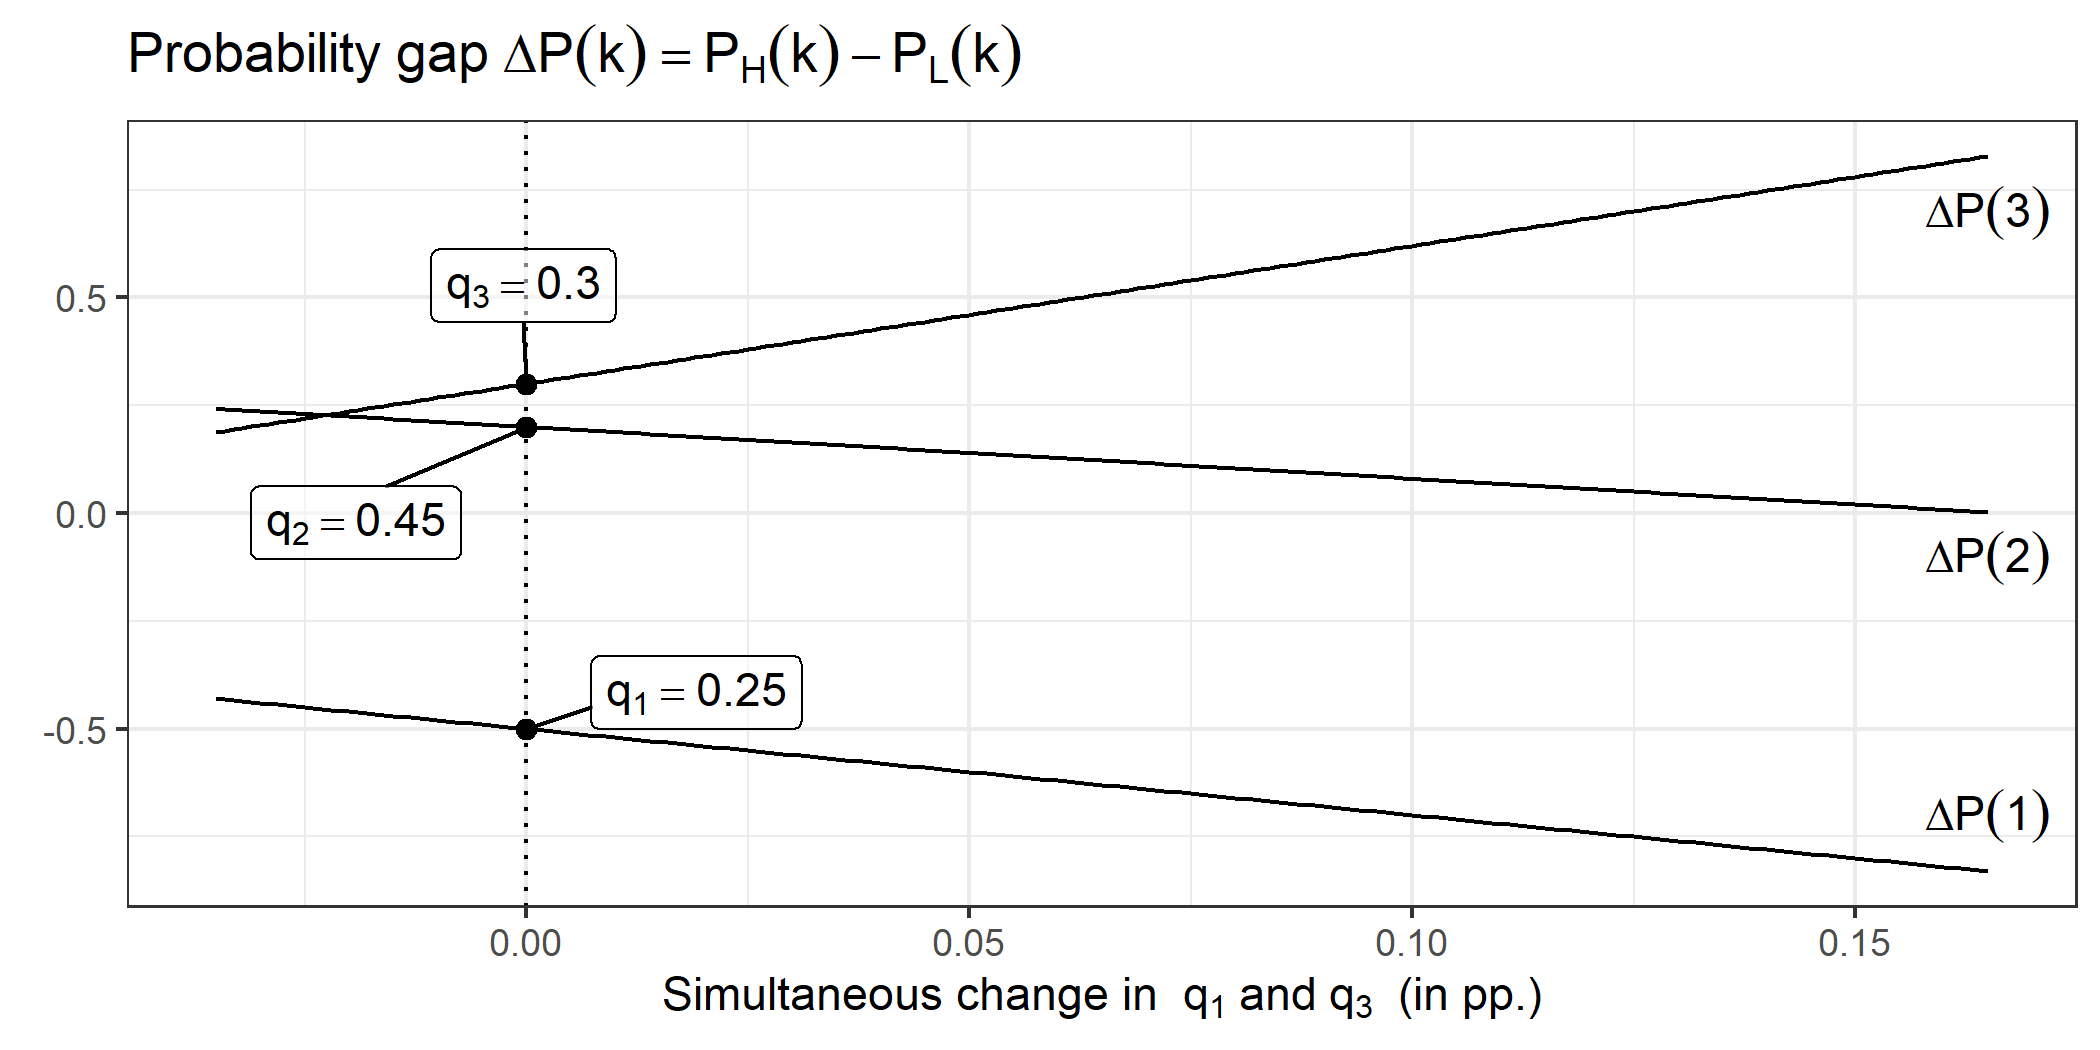
\includegraphics[width=\linewidth]{chap2/graphic/theory-proba-gap.png}
	\vspace{-3em}
	\justify\singlespacing\footnotesize{\textit{Notes:} This figure presents the probability gap in second-period occupations between children from $H$ and $L$ parental income, i.e. $\Delta P(k)$, according to changes in the share of low- and high-paying jobs, i.e. $q_1$ and $q_3$.
	Changes in $q_1$ and $q_3$ are of equal magnitude and at the expense of $q_2$ since $q_1+q_2+q_3=1$.
	Parameters of the model are set such that $z_L = 0.5$, $z_H = 0.5$, and $\pi = 0.25$. The dotted line represents the baseline occupational distribution where $q_1=0.3$, $q_2=0.45$, and $q_3=0.25$.}
\end{figure}
The initial distribution of occupations is assumed to be such that 25\% of workers are in low-paying, 45\% in middling, and 30\% in high-paying occupations. These are figures close to those found in the data, as we will see below. To capture polarization we increase simultaneously $q_{1}$ and $q_{3}$ by the same amount, reducing $q_2$ until only 15\% of workers are in middling occupations (and 40\% and 45\% in $q_1$ and $ q_3$ respectively). The horizontal axis depicts the change in $q_{1}$ and $q_{3}$ in percentage points.

The figure indicates that as polarization increases the advantage in accessing high-paying occupation that those from high-income background have relative to those from low-income households rises. The opposite occurs with low-paying occupations, where the relative likelihood of being in such jobs (which is negative, as only $L$-workers are employed in occupation 1) grows in absolute value with polarization. $H$-workers also have an advantage in being in occupation 2 for low level of polarization, but this advantage falls as $q_1$ and $q_3$ increase, and for high levels of polarization there are more $L$-workers than $H$-workers in middling jobs. The reason for this is that as $q_1$ increases, fewer high-ability $L$-workers manage to move to high-paying occupations, raising their likelihood to be in middling occupations and increasing the number of high-paying jobs available for low-ability $H$-workers. \footnote{In the Appendix we examine separately the effect of changes in $q_1$ and $q_3$ and show that an increase in either of them tends to raise the probability gap between the two types of workers.}

Our results imply a negative relationship between the extent of polarization and the degree of occupation mobility. Greater employment polarization---as measured by an increase in $q_{1}$ and $q_{3}$---reduces mobility by making the distribution of occupations of mature workers more dependent on parental background. This relationship could exist both over time or across locations. If two cohorts of workers face different degrees of polarization when they enter the labour market, we expect to find a lower degree of mobility for the one that experienced a lower share of middling jobs. Similarly, when comparing workers in two geographical areas, we expect to find lower mobility for those based in the location where polarization is greatest.
    
    \section{Data and employment polarization} \label{chap2-data}
    \subsection{Sample and variables}

We use two mature British cohort studies that have been widely used by economists and sociologists to examine the extent of mobility in the UK. The National Child Development Study (NCDS58) is a cohort of individuals born during a given week in March 1958. The British Cohort Study (BCS70) is composed of individuals born during a given week in April 1970. Cohort members were born in England, Scotland, Wales and Northern Ireland and participated in several interviews at different points in time over their life. 
\begin{figure}[!tb]
    \centering
    \caption{Dates of interviews}
    \label{chap2-fig:interviews}
    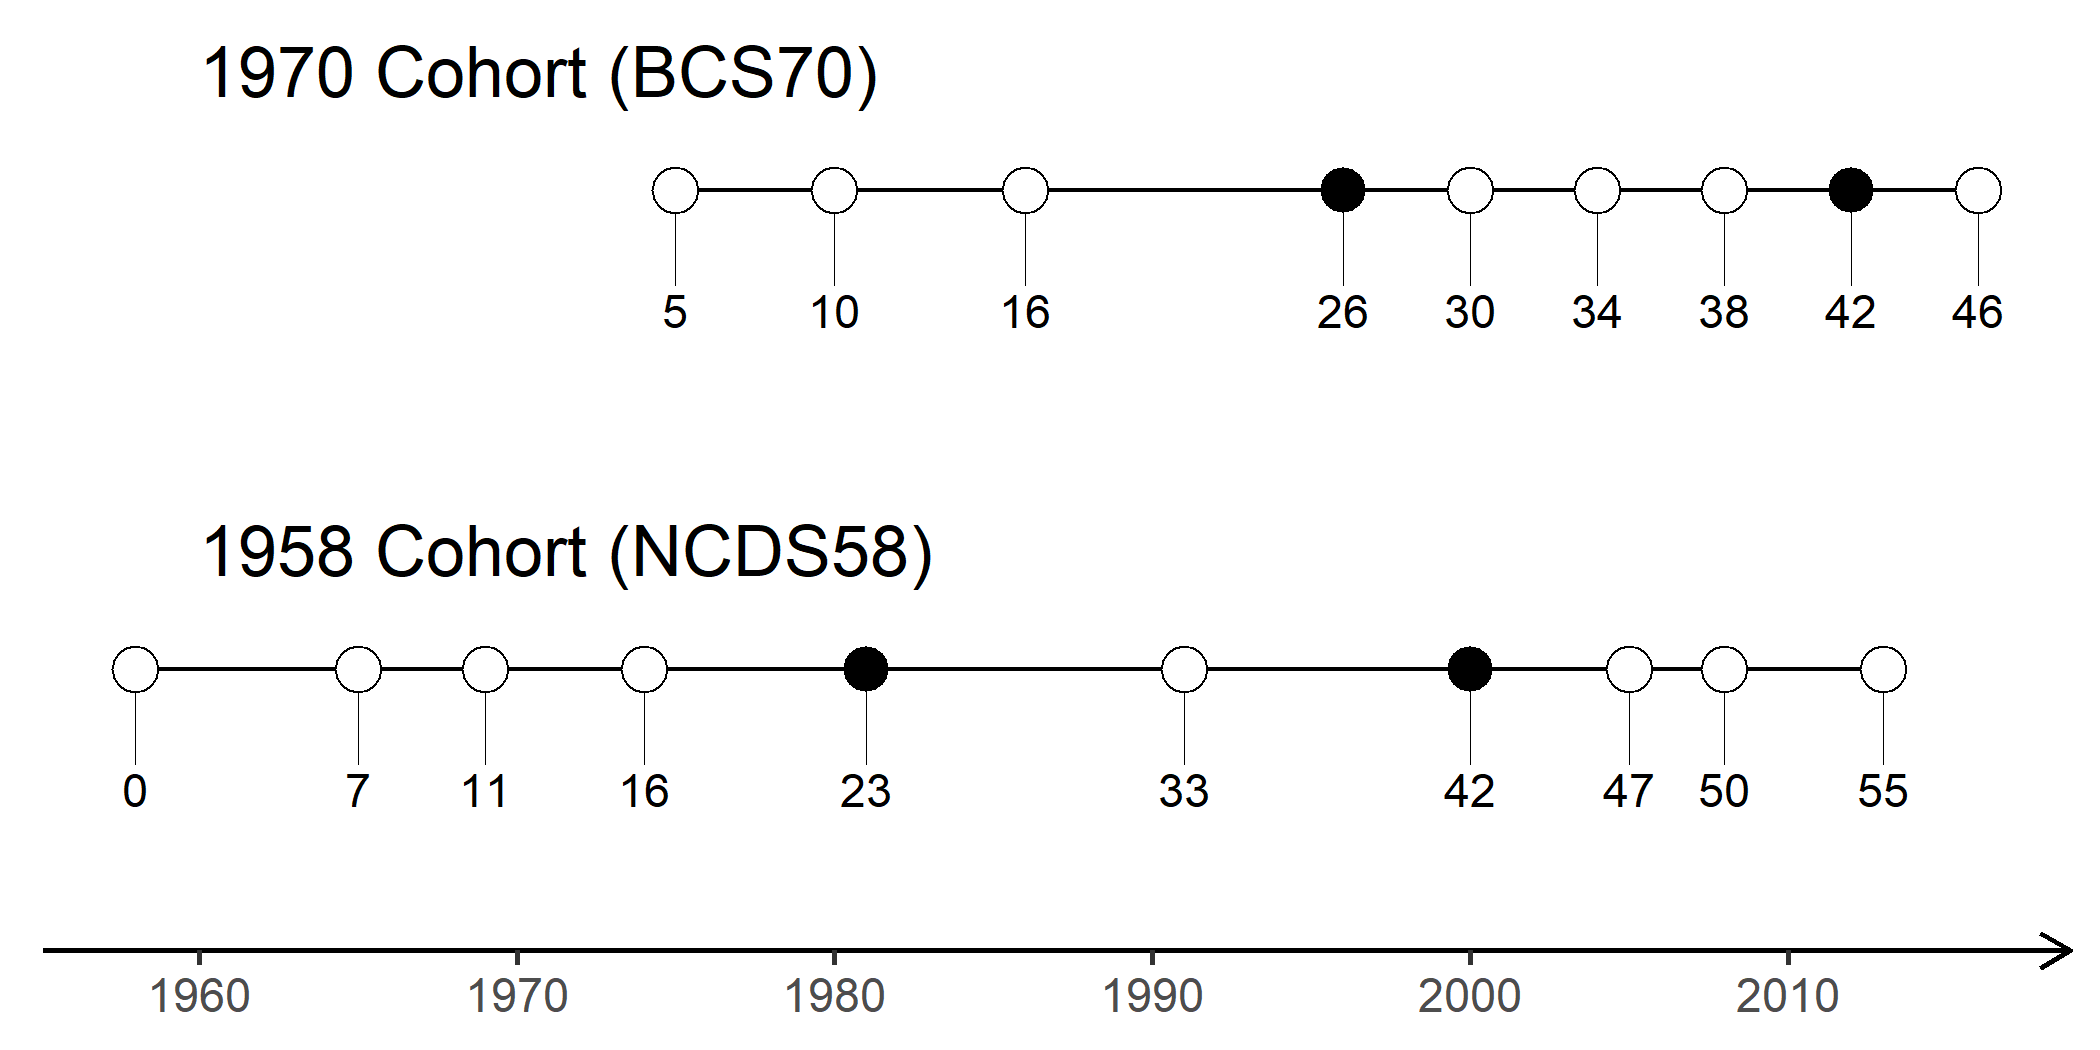
\includegraphics[width=\linewidth]{chap2/graphic/itw-date-spreadpol.png}
	\vspace{-3em}
	\justify\singlespacing\footnotesize{\textit{Notes:} This figure presents the dates at which individuals in the BCS70 and NCDS58 cohorts may have been interviewed and the corresponding years. Black circles represent the first and second periods we consider in the analysis for both cohorts.}
\end{figure}
Figure \ref{chap2-fig:interviews} presents all the interviews at which cohort members were interviewed and the corresponding year.

\textbf{Periods.} We define the first period as the year of interview closest to that in which the individual was 25 years-old, the age usually considered as that of entry into the labour market. Those in the NCDS58 cohort are observed at age 23 and those in the BCS70 cohort at age 26. Both cohorts are interviewed at age 42, which we define as the second period.

\textbf{Income and wages.} We have information on parental income, which is provided when the child was 16 years-old for both cohorts. For the BCS70 cohort, it is also available when the child was 10. Thus, when both are available, we take the average of the two observations; otherwise we use the single one we observe.\footnote{\cite{Blanden2013Intergenerational} show that the observed increase in the role of parental income to determine child's income is not driven by the poor measurement of permanent income in the 1958 cohort.} In order to adjust both for inflation, aggregate income growth and changes in the dispersion of income, parental income is standardized, so that for both cohorts it has mean zero and a variance of 1 (see Table \ref{chap2-tab:stat-indiv} for the summary statistics).

For children, we observe wages, which are reported at each wave. We adjust for inflation using the consumer price index provided by the \href{https://www.ons.gov.uk/economy/inflationandpriceindices}{UK Office for National Statistics}. The resulting monetary variables are all expressed in 1970 British pounds. 

% International Standard Classification of Occupations 1988 (ISCO-88)
\textbf{Occupational categories.} Both cohorts studies provide the full activity histories to the nearest month from which we can derive the ISCO-88 occupations.\footnote{Cohort data provide 3-digit occupations in the \href{https://www.hesa.ac.uk/support/documentation/occupational/soc90}{Standard Occupational Classification 1990 (SOC90)} and the \href{https://www.hesa.ac.uk/support/documentation/occupational/soc2000}{Standard Occupational Classification 2000 (SOC2000)}. We can derive ISCO-88 occupations by using the files from \href{http://www.camsis.stir.ac.uk/occunits/distribution.html}{CAMSIS project} which cover both SOC occupational unit codes and translations into ISCO-88.}
We aggregate ISCO-88 occupations into three categories: high-paying, middling and low-paying occupations. This classification follows the job-polarization literature and is consistent with that used in \cite{Goos2014Explaining} and \cite{Mahutga2018Job}.\footnote{A large body of literature on social mobility relies on the National Statistics Socio-Economic Classification (NS-SEC), starting with \cite{Erikson1992Constant} and \cite{Rose1998ESRC}. However, such classification uses a definition of routine occupations that does not match that used in the job-polarization literature. For instance, the NS-SEC considers that an employee in the 3-digit occupation \textit{Bar staff (622)} has a routine occupation. However, it cannot be considered as a routine job following the definition of \cite{Autor2003Skill} who define this type of job as a non-routine interactive job. We hence chose not to rely on the NS-SEC for our analysis.} Table \ref{chap2-tab:data-isco88} in the appendix presents the classification.  For completeness, we also include a fourth category---individuals who are out-of-work. This category groups those out of the labour force, those who are unemployed, and those in full-time study. Table \ref{chap2-tab:stat-cohper} displays the shares of the various activity status and occupational categories in the cohort data.

As has been shown in previous work, occupational categories are closely related to remuneration levels, and we document this for our cohort data in the appendix. Table \ref{chap2-tab:stat-pay} reports the average weekly pay by occupation, and displays the expected correlation between occupations and pay. 

\textbf{Location.} Since individuals give their address at each interview, we also have their location history. We focus on the region of residence at the age of 16 because it is the age at which the parental income variable is defined. The classification is prior to 1994 and thus uses the Government Offices for the Regions (GORs). We therefore rely on the Standard Statistical Regions (SSR).\footnote{For England, this is the highest sub-national division, while the other countries in Britain consists of a single region. The regions are (in alphabetical order): East Anglia, East Midlands, North, North West, Scotland, South East, South West, Wales, West Midlands, and Yorkshire and Humberside.} Table \ref{chap2-tab:stat-location} reports the share of cohort members in each region for both periods.

Once we restrict the data to those individuals for whom we have the key characteristics, i.e. parental income and occupations, our sample consists of 6,780 individuals in the NCDS58 and 7,983 in the BCS70, as reported in Table \ref{chap2-tab:stat-indiv}.

\textbf{The Labour Force Survey.} As a complementary dataset we use the Labor Force Survey (LFS). The LFS provides data on both labour market status and region of residence. It has the advantage of containing a much larger number of observations (see Appendix \ref{chap2-app-data-LFS} for the details), and allows us to compare the changes in the occupational structure in the cohort data with those from a larger sample, as well as to compute measures of polarization at the regional level.


\subsection{The structure of employment}

% Contribution - alternative view of polarization to the usual snapshot
Before proceeding to our empirical analysis, we consider the extent to which the two cohorts experienced different degrees of polarization. We start by looking at the change in the distribution of occupations at ages 23/26 and 42 for both cohorts, reported in Figure \ref{chap2-fig:stat-occ}.\footnote{We report the proportion of individuals in each occupation for the two cohorts in Tables \ref{chap2-tab:proba-group4-abs} and \ref{chap2-tab:proba-group5-abs} in the appendix.} In the first period there is an increase across cohorts in the probability of working in a high- and low-paying occupation and a decline in that of working in a middling-paying occupation. When we consider the occupations at age 42, the changes are of smaller magnitude, and the main difference across the two cohorts is a reduction in the share of middling jobs that has been offset by high-paying ones. These changes are consistent with the literature on polarization in the UK that shows a considerable decline in middling jobs, and an increase in the other two categories, which is particularly large for high-paying jobs (see Figure \ref{chap2-fig:lfs-national} in the appendix). The differences between the first and second period distributions are interesting for our purposes, as they raise the question of whether polarization in the first period matters even when the changes in the distribution of employment are small for mature individuals. 
\begin{figure}[!tb]
    \centering
    \caption{Occupation distribution across cohorts}
    \label{chap2-fig:stat-occ}
    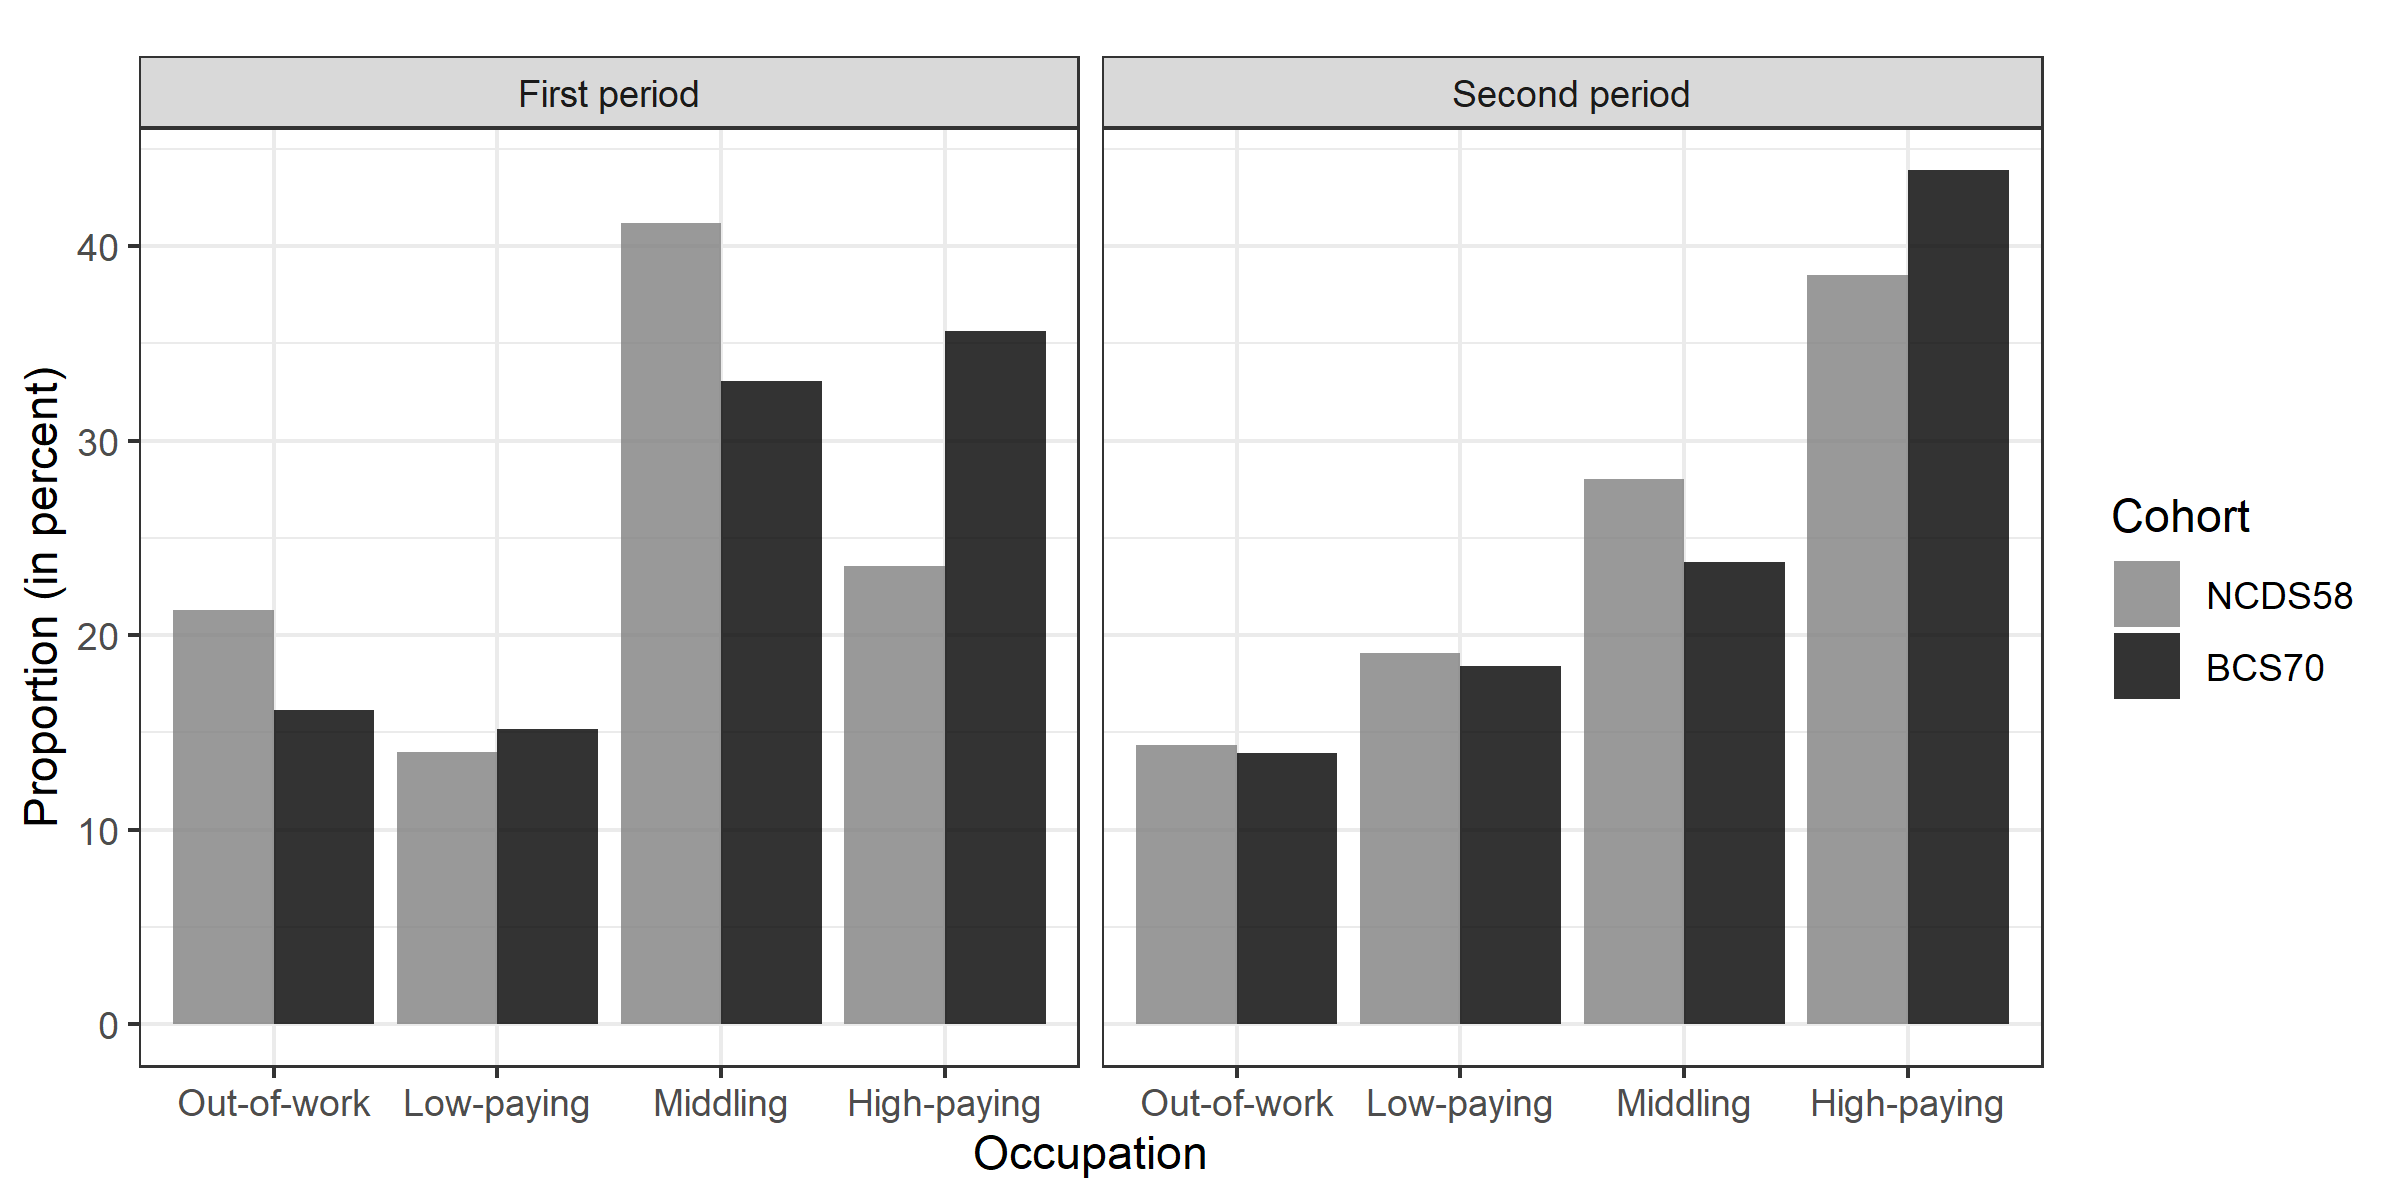
\includegraphics[width=\linewidth]{chap2/graphic/stat-occ.png}
	\vspace{-3em}
	\justify\singlespacing\footnotesize{\textit{Notes:} This figure reports the proportion of individuals, expressed in percent, in each type of occupation (out-of-work, low-paying, middling, high-paying) for the NCDS58 and BCS70 cohorts according to the period.}
\end{figure}
To better understand these dynamics, Figure \ref{chap2-fig:polarize-isco88-both} in the Appendix performs a similar exercise using the ISCO-88 categories, and shows a clear pattern of polarization, which has been particularly large for young individual.

As an alternative way of thinking about polarization we examine how occupations with either different average pay or  ``routine task intensity'' (RTI) have changed across the two cohorts, reported in Figure \ref{chap2-fig:polarize-both-p1}. The left panel depicts the change in the share of individuals in each occupation when young and plots it against the average pay in that occupation (for young individuals of the 1970 cohort). The occupations are depicted by both their code and a geometric symbol, were the latter indicate whether they are in our category of low-paying (circle), middling (triangle) or high-paying (square) occupations. As can be seen from the fitted curve, there is a U-shaped relationship between weekly pay and the change in the share of the occupation, with both those with low and those with high remuneration gaining employment shares at the expense of those in the middle.
\begin{figure}[!tb]
    \centering
    \caption{Change in the probability of being in each ISCO-88 occupation in the first period}
    \label{chap2-fig:polarize-both-p1}
    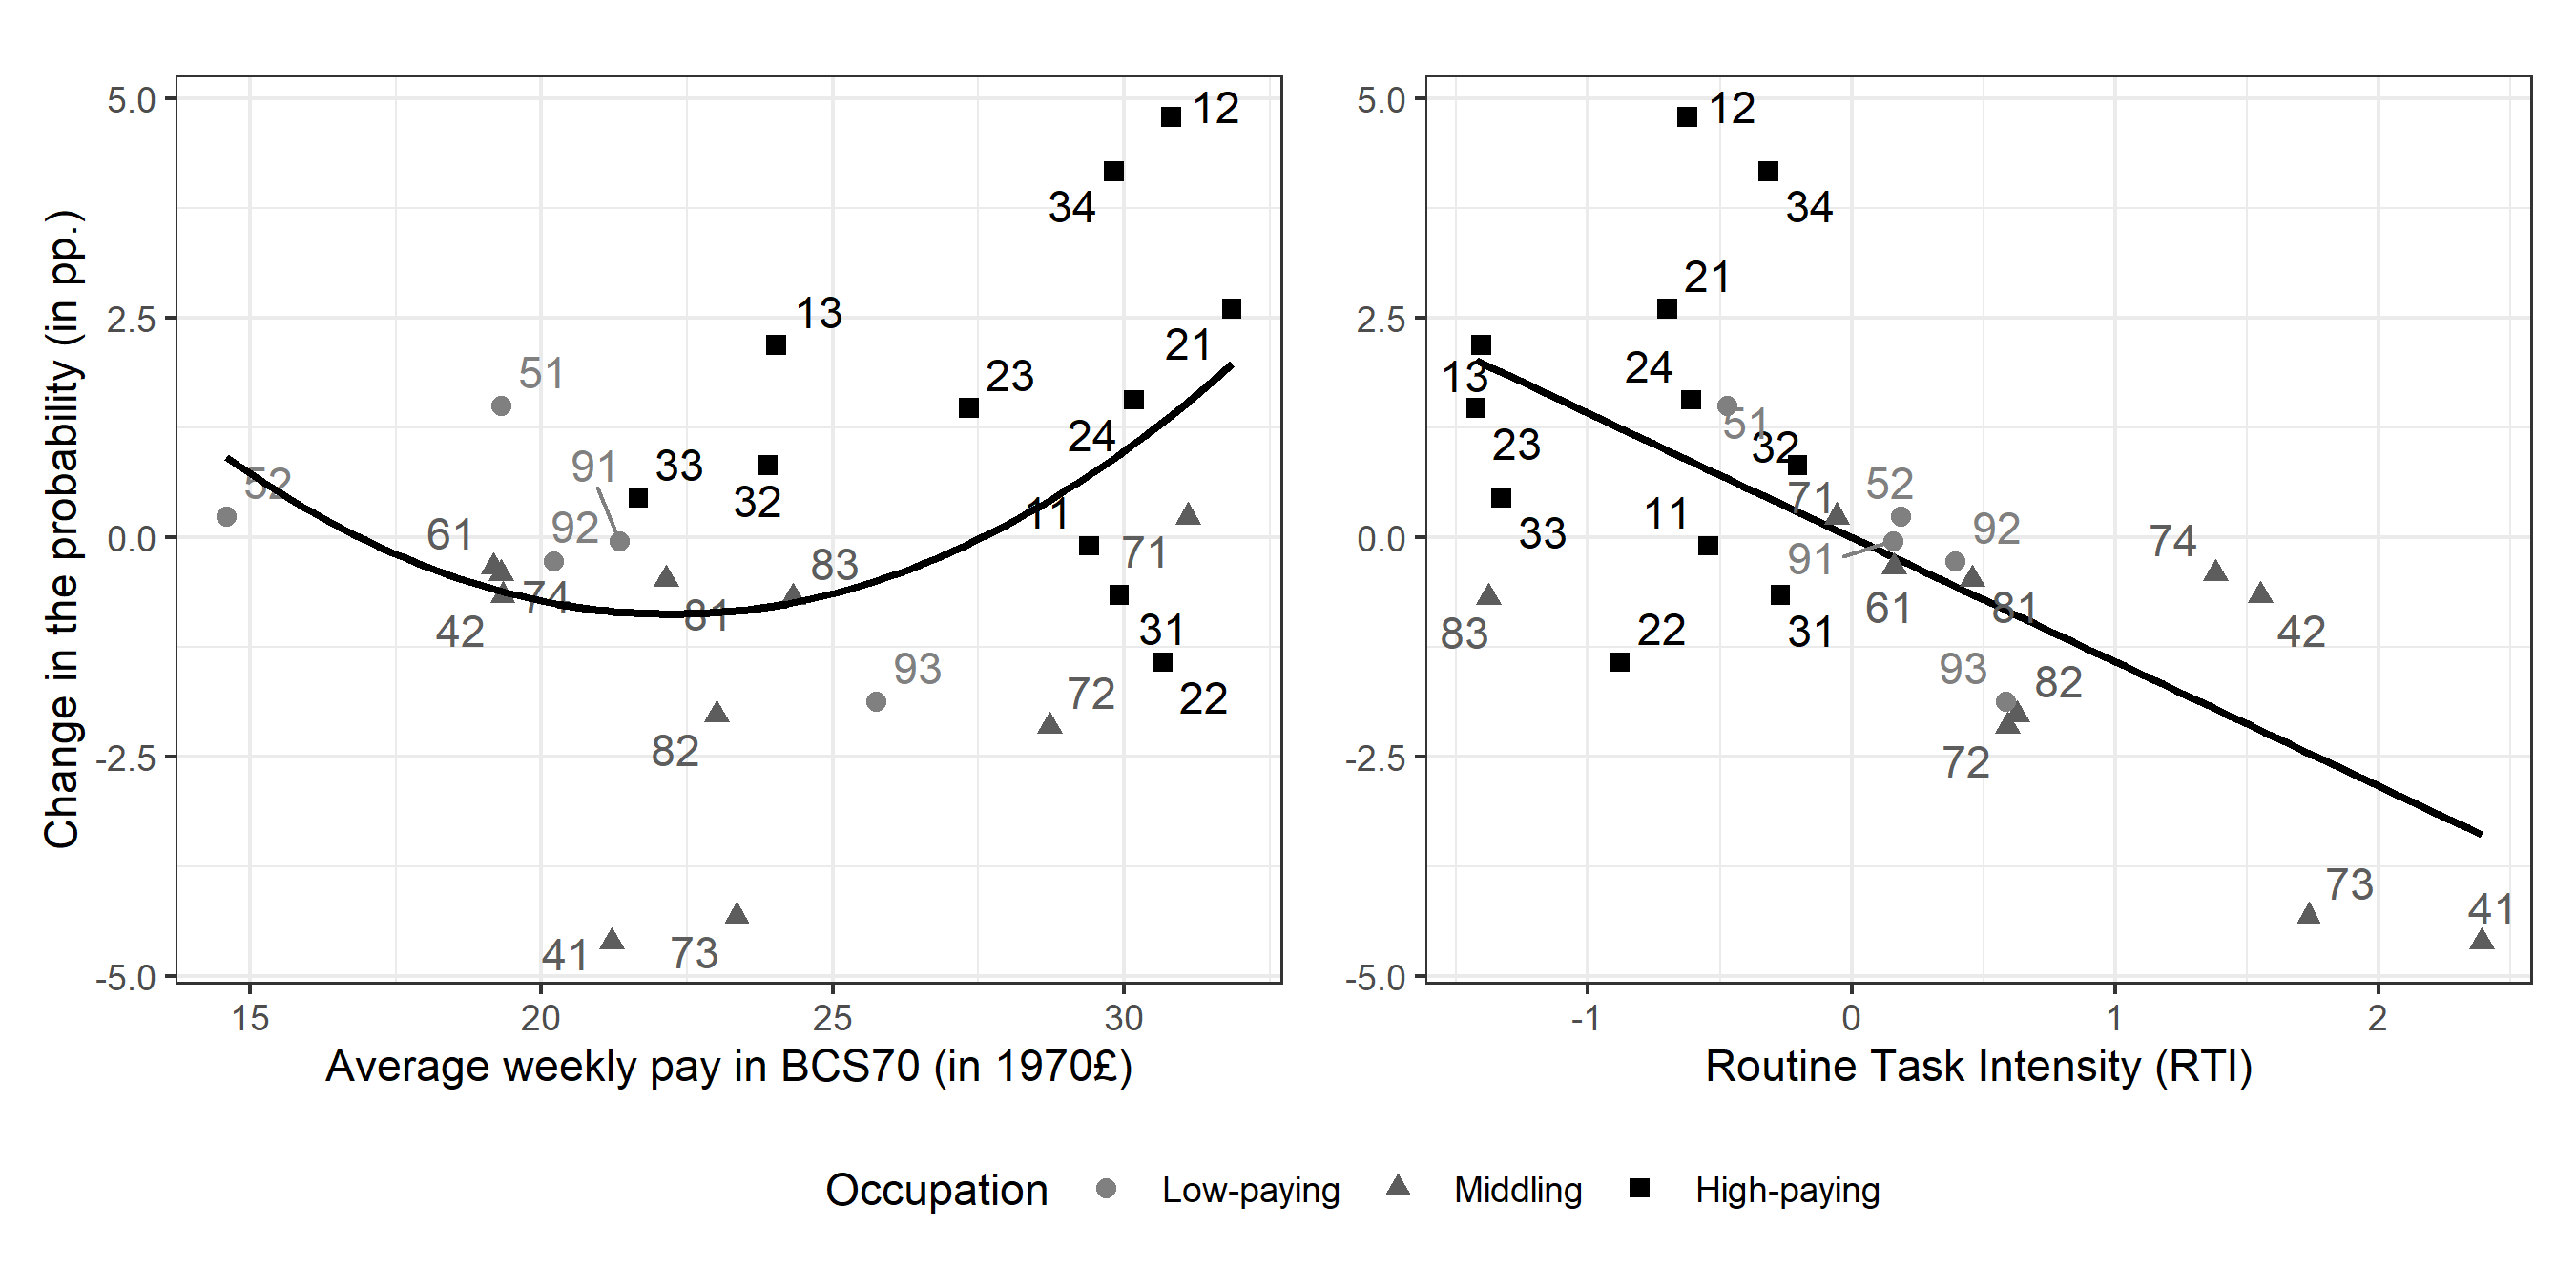
\includegraphics[width=\linewidth]{chap2/graphic/polarize-both-p1.png}
	\vspace{-3em}
	\justify\singlespacing\footnotesize{\textit{Notes:} The left-hand side panel of the figure presents the U-shaped relationship between the difference, expressed in percentage points, between the BCS70 and NCDS58 cohorts in terms of probability of being in each ISCO-88 occupation in the first period and the average weekly pay, expressed in 1970\pounds, in this occupation for the BCS70 cohort. The right-hand side panel shows the negative relationship between the difference, expressed in percentage points, between the BCS70 and NCDS58 cohorts in terms of probability of being in each ISCO-88 occupation in first period and the Routine Task Intensity (RTI) index from \cite{Mahutga2018Job}.}
\end{figure}
The right panel plots the change in the share of each occupation for young individuals against the RTI index provided by \cite{Mahutga2018Job}. The downward slopping line in Figure \ref{chap2-fig:polarize-both-p1} corresponds to the fitted curve implied by the data, and indicates that the change is negatively correlated with the degree of routinization. 

The various pieces of evidence in this section thus indicate that the strong polarization identified in cross-sectional data by previous work is also present when we focus on two specific cohorts. Routine intensity seems to be highly correlated with changes in the share of occupations, with low RTI ones having gained share and those with high RTI having lost it. Moreover, polarization appears whether we use the RTI index to categorize occupations or when we look at average weekly pay.

\subsection{Occupational dynamics} \label{chap2-dynamics}

While the literature on inter-generational mobility has traditionally focused on the outcomes of children when they are mature, we are interested in the occupational dynamics through which individuals reach a particular outcome. To illustrate why this is important, Table \ref{chap2-tab:proba-group4-cdt} reports the conditional probabilities of switching occupations between age 23/26 and age 42.\footnote{To understand why the probability of moving from out-of-work into a high-paying occupation is so high, recall that the former category includes those in education. Conditional probabilities in which we consider those in education as separate category, hence not included in out-of-work, are reported in the appendix, and display the expected (large) difference between those in education and the rest of those out-of-work; see Table \ref{chap2-tab:proba-group5-cdt-short}.}

\begin{table}[!tb]
    \centering
    \caption{Conditional probabilities of changing occupations}
    \label{chap2-tab:proba-group4-cdt}
    \begin{threeparttable}
        \small
        
\begin{tabular}{lrrrrrrrr}
\toprule
\multicolumn{1}{c}{} & \multicolumn{4}{c}{BCS70} & \multicolumn{4}{c}{NCDS58} \\
\cmidrule(l{3pt}r{3pt}){2-5} \cmidrule(l{3pt}r{3pt}){6-9}
Occupation & Out & Low & Mid & High & Out & Low & Mid & High\\
\midrule
Out-of-work & 33.8 & 25.3 & 14.5 & 26.4 & 27.4 & 24.7 & 20.7 & 27.3\\
Low-paying & 13.6 & 45.1 & 17.5 & 23.8 & 16.3 & 40.0 & 20.3 & 23.4\\
Middling & 10.5 & 13.8 & 44.9 & 30.8 & 10.4 & 15.4 & 43.4 & 30.8\\
High-paying & 8.3 & 8.2 & 11.0 & 72.6 & 8.5 & 8.1 & 12.3 & 71.2\\
\bottomrule
\end{tabular}

        \begin{tablenotes}[flushleft]
            \footnotesize{\item \textit{Notes}: This table shows the probability, expressed in percent, of being in each second-period occupation (columns) conditional on the first-period occupation (rows) for individuals in the NCDS58 and BCS70 cohorts.}
        \end{tablenotes}
    \end{threeparttable}
\end{table}

The table shows that there is a considerable degree of mobility across occupations over the individual's lifetime, i.e. of intra-generational mobility. Individuals who start their careers in low-paying and middling occupations have probabilities of staying there of around 40\% and a substantial likelihood of moving upwards. Notably, 30.8\% of those initially in middling occupations have a job in high-paying occupations by age 42 for both cohorts. In contrast, persistence is high for those who start in high-paying occupations, over 70\%. The transition probabilities are remarkably similar across cohorts, in particular those of moving into a high-paying occupation. The most significant differences come from the outcomes of those who start either out of work or in low-paying occupations. In both cases, those in the younger cohort face a lower probability of being in a middling occupation when mature (lower by 5.8 and 2.5 pp., respectively) which translates into higher odds of remaining in the occupation of origin. 

These figures indicate that the occupational outcomes of mature individuals depend both on their initial occupations and on the transitions across occupations, and raise the question of whether a reduction in the share of middling jobs can be a break to mobility. If mobility occurs partly through individuals progressing up the income ladder during their careers, the disappearance of middling jobs can have important consequences. On the one hand, a large proportion of those who are in high-paying occupations at age 42 start their careers in middling occupations. If fewer individuals are in such occupations when young, as indicated by Figure \ref{chap2-fig:stat-occ}, then there will be fewer individuals that can move into high-paying jobs. On the other, those who start in low-paying occupations have access to fewer middling jobs and hence are more likely to stay in their initial occupations. The importance of such changes for mobility will depend on the extent to which parental background matters for entry into each occupation and for the subsequent dynamics.

    
    \section{Empirical specification} \label{chap2-specification}
    Our analysis proceeds in two steps. The first consists in examining how an individual's occupation is affected by parental background. As we will detail in the next subsection, we suppose that this impact can potentially occur both through the effect on the child's initial occupation and on her occupation as a mature worker. In a second step, we consider regional patterns of mobility and assess to what extent regional differences in polarization are correlated to observed mobility patterns at the regional level.

\subsection{The determinants of individual mobility} \label{chap2-specification1}

In order to understand the effect of parental income on occupational dynamics we start by estimating its impact on the child's probability to start her career in each occupation $j\in J = \{O, L , M, H\}$, where the possible occupations are out-of-work ($O$), low-paying ($L$), middling ($M$) and high-paying ($H$). We define the out-of-work occupation as the baseline occupation category. Let $p_j$ be the probability to start in occupation $j = \{L , M, H\}$ which is given by the following multinomial logistic model:
\begin{equation}\label{chap2-eq:emp-multi1}
    \log\left(\frac{p_j}{p_O}\right) = \alpha_{1j} + \beta_{1j} Y^p + \gamma_{1j} X,
\end{equation}
where $Y^p$ is parental income, and $X$ are individual characteristics (in our baseline specifications simply gender). Parental income is log-standardized. All terms will be interacted with a dummy that equals one for those in the 1970 cohort (BCS70) and zero otherwise. Cross-term coefficients hence represent the change across cohorts in the effect of the variable on the child's initial occupation. In the appendix, we also report the estimation of the four binomial logistic models that characterize the multinomial one.

We next consider the determinants of the probability of being in occupation $k \in K = \{O, L , M, H\}$ at age 42. The simplest specification is to consider a specification of the form
\begin{equation}\label{chap2-eq:emp-multi2}
    \log\left(\frac{p_k}{p_O}\right) = \alpha_{2k} + \beta_{2k} Y^p + \gamma_{2k} X,
\end{equation}
which captures how parental income determines the occupational outcome of the mature child. This expression is consistent with the approach usually found in the literature on inter-generational mobility in which only the labour market outcome of the mature worker is considered. In contrast, intra-generational analyses have focused on how incomes evolve over the individual's working life. We hence consider the following specification: 
\begin{equation}\label{chap2-eq:emp-multi3}
    \log\left(\frac{p_k}{p_O}\right) = \alpha_{3k} + \sum_{j} \eta_{kj} \mathbb{1}_{j} + \beta_{3k} Y^p + \gamma_{3k} X,
\end{equation}
where $\mathbb{1}_{j}$ is a dummy variable that equals one when the individual was in occupation $j\in J$ when young. As before, we estimate second-period equations with a multinomial model and separately for the four occupations using binomial logistic regressions, which we report in the appendix.

The expression in equation (\ref{chap2-eq:emp-multi3}) shares with the literature on intra-generational mobility the idea that individual's may change position in the income ladder and that it is important to understand how those dynamics operate. It differs from existing approaches in two respects. First, we focus on occupational mobility over the lifetime, rather than income mobility; second, we control for parental income as a potential factor that can influence the extent to which the child changes occupations over time. Equation (\ref{chap2-eq:emp-multi3}) then adds to the literature on intra-generational mobility by allowing parental income to have an impact on lifetime occupational changes, and to that on inter-generational mobility by allowing the effect of parental income on the occupation of mature workers to occur both through their initial occupation and through the likelihood of transition to other jobs.  

Our empirical strategy makes two important choices. The first is not to consider education decisions and to focus exclusively on the direct impact of parental income. The alternative approach would be to consider a three-step setup in which parental income determines education, which then determines first-period occupation, which in turn determines the second-period job.\footnote{A large literature has considered the role of education for social mobility, and in particular examined to what extent the influence of parental background takes place through educational achievement. Examples of this literature are \cite{Blanden2004Family}, \cite{Blanden2014Education}, \cite{Blanden2016Educational}, \cite{Gregg2010Family} and \cite{Major2018Social}.} The advantage of the latter approach is that it would allow us to infer how much of the parental-income advantage operates through education and how much is a direct effect; the drawback is that educational attainment is correlated with unobservable characteristics, notably ability but also the type of school attended, hence the effect that we may be attributing to years of education could be capturing other aspects, whether innate or related to parental background.\footnote{See \cite{harmon2003returns} for a discussion of the difficulty of differentiating between the returns to education and those to (innate or socially-acquired) ability.} We hence focus exclusively on the two occupational outcomes, although we perform the three-step analysis in Appendix \ref{chap2-app-education}.

Second, we have chosen to use a multinomial logistic model considering the four possible occupational outcomes and where our reference outcome is being out-of-work. It is important to note that the transition from this category into the three employment occupations occurs with roughly equal probabilities. Notably, for the NCDS58 (BSC70) the probability of transiting from out of work to low- and high-paying occupations was, respectively, 24.7 pp. (25.3 pp.) and 27.3 pp. (26.4 pp.), i.e. of very similar magnitude. The likelihood to move into middling occupations was somewhat lower (20.7 and 14.5 pp.) but of comparable magnitude; see Table \ref{chap2-tab:proba-group4-cdt} above.

\subsection{Mobility and regional polarization}

The second step of our analysis consists in exploring the relationship between the observed changes in the role of parental income and polarization. We do so by examining whether changes in regional mobility are correlated to changes in the extent of polarization at the regional level. To do so we run a multinomial regression at the regional level for the determinants of the probability of being in occupation $k \in K = \{O, L , M, H\}$ at age 42. We do not compute first-period mobility and conditional second-period mobility because of sample sizes, as in many regions we have only a small number of individuals moving across certain occupations between first and second period. The equation we estimate is hence
\begin{equation}\label{chap2-eq:regocc-multi2}
    \log\left(\frac{p^r_k}{p^r_O}\right) = \alpha^r_{k} + \beta^r_{k} Y^p + \gamma^r_{k} X,
\end{equation}
where \emph{r} denotes the region. We hence use individual data to estimate 10 coefficients $\beta^r_{k}$ that capture the impact of parental income on occupational outcomes in each of the regions.

As we will see below, our estimates indicate that the dynamics of the impact of parental income vary across regions, with the change across generations being much larger in some than in others. The last step in our analysis is hence to construct a measure of regional polarization and compute its correlation with our regional estimates. To capture changes in mobility in region $r$, we consider the between-cohort change in the role of parental income for being in occupation $k$, namely, $\Delta\beta_k^r$. We hence compute the correlation between mobility and polarization by running the regression
\begin{equation}\label{chap2-eq:reg-multi2}
    \Delta\beta_k^r = \delta_{k} + \eta_{k} \Delta Pol^r,
\end{equation}
where $Pol^r$ is a measure of polarization at the regional level for a particular cohort and $\Delta Pol^r$ its change across cohorts. The measure of polarization will be constructed using the Labour Force Survey in order to have larger regional samples than those provided by the cohort data \footnote{The measure of polarization used is discussed is detail in section \ref{chap2-regional} below, and Appendix \ref{chap2-app-data-LFS} gives details on the data used.} 








    
    \section{Patterns of mobility} \label{chap2-mobility}
    \subsection{Initial occupations} \label{chap2-initial}

We start by estimating the impact of parental income on the child's first-period occupations, before considering the occupation of mature individuals in the next section. We estimate equation \eqref{chap2-eq:emp-multi1} and report the results in the appendix, those for the binomial logits are reported in Table \ref{chap2-tab:occ-bi1-base} and the multinomial results in Table \ref{chap2-tab:occ-multi1-base}.  Logit coefficients are hard to interpret, hence to visualize the results Figure \ref{chap2-fig:occ-multi1-pinc} displays the probability to be in each occupation when young as a function of parental income.
\begin{figure}[!tb]
    \centering
    \caption{First-period occupation probability according to parental income}
    \label{chap2-fig:occ-multi1-pinc}
    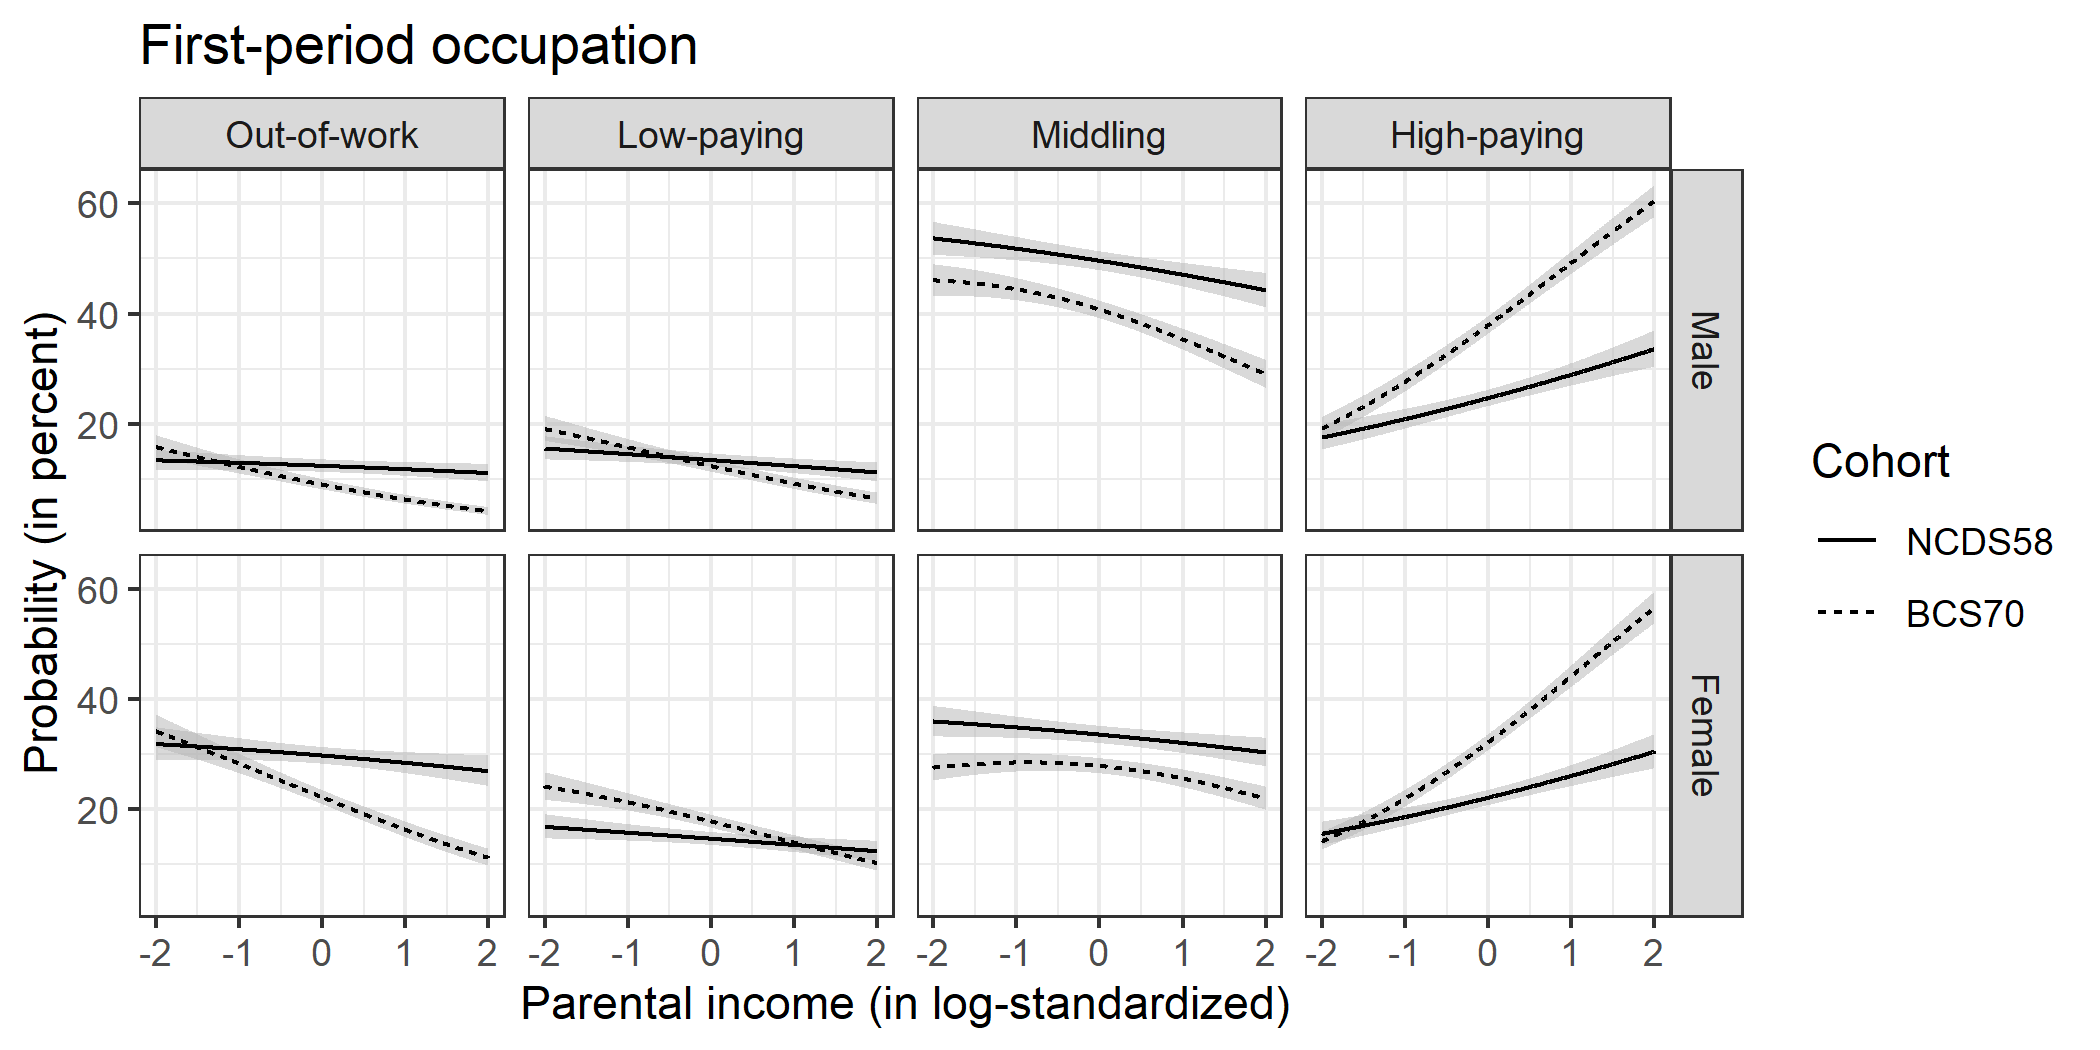
\includegraphics[width=\linewidth]{chap2/graphic/occ-multi1-pinc.png}
    \vspace{-3em}
	\justify\singlespacing\footnotesize{\textit{Notes:} This figure presents the probability, expressed in percent, of being in each type of occupation (out-of-work, low-paying, middling, high-paying) in first period according to parental income, in log-standardized.
	Probabilities are computed for males and females in both cohorts according to the multinomial logistic regression reported in Table \ref{chap2-tab:occ-multi1-base} in the appendix.}
\end{figure}
The probabilities are computed according to the multinomial logistic regression, but the results are qualitatively equivalent when using the binomial estimates. The probabilities are reported separately for the two cohorts and for the two genders; the four columns depict the four possible outcomes, starting with out-of-work occupations on the left.

Consider first the outcomes for the 1958 cohort, depicted by the continuous lines. Parental income is a key determinant of initial occupation, with high income increasing the probability to be in a high-paying occupation and reducing that of being in a middling or low-paying one. There is no effect on the probability of being out-of-work (see also Table \ref{chap2-tab:occ-bi1-base}), a result that is not surprising given the various outcomes included in this category. Note also that the effect of family background is particularly large for high-paying occupations. The levels vary across men and women, with women being more likely than men to be out-of-work and less likely to be in any of the three types of employment.

The impact of parental income on the various probabilities for the 1970 cohort are depicted by the dashed lines. Starting with men, Table \ref{chap2-tab:occ-multi1-base} reports large changes across cohorts in the coefficients on the direct effect of parental income, which are captured in the figures. For example, the coefficient doubles for high-paying occupations, increasing from 0.21 to 0.41, a result that is reflected in the large increase in the slope of the schedule that we observe in the two right panels. There are various possible explanations for this. Obviously, the effect could be operating through education which has become more dependent on parental background (see Appendix \ref{chap2-app-education} for a discussion). Other explanations are that non-cognitive skills have become more important and that they are positively associated with the household’s income, or parental income could be a proxy for the child’s social network, either its size or ‘quality’, which in turn has become more important in determining access to jobs.\footnote{For example, \cite{Blanden2007Accounting}, using the same data as us, show a strengthening of the relationship between parental income and non-cognitive skills between both cohorts. \cite{Major2018Social} emphasize the changing role of education and the increasing importance of the "extra-investments" made by upper-middle class families. For the US, \cite{Chetty2014Land} show that neighborhood characteristics are extensively correlated with mobility.}

As expected, the probability of being in a middling occupation has fallen for all individuals, irrespective of family background. The decline has been greater the higher parental income is. Together with the previous result this indicates that as the share of high-paying jobs increased, those from high-income households are more likely to go into high-paying jobs at the expense of middling ones. The probability of being in a low-paying occupation has pivoted around the mean, with those at the bottom (resp. top) of the parental income distribution being more (resp. less) likely to be in that occupation in the 1970 than in the 1958 cohort. The schedule for being out of work displays a steeper slope, with a decline in the probability of being in this category for all men except those at the very bottom of the parental income distribution.

Consider now the schedules for women. Starting from the right, we can see that women experienced a large decline in the likelihood of being out-of-work, consistent with the increase in female labour force participation observed over the period. Yet, the reduction is strongly correlated to parental income, even more so than for men. The probability of being in a low-paying occupation has increased at virtually all points of the distribution---except at the very top---indicating that much of the increase in female participation occurred through access to low-paying jobs. The probability of being in middling occupations has declined for the younger cohort, as is the case for men. Interestingly, for women the schedule is non-monotonic. At the bottom of the parental income distribution, an increase be income raises the probability of being in middle occupations, with the effect then turning negative. This seems to indicate that in the lower segment of the parental income distribution, an increase in income confers women a occupational advantage, allowing them to access middling rather than low-paying jobs. As is the case for men, the slope of the schedule for high-paying occupations has increased sharply across the two cohorts.

These patterns indicate that parental income conferred a greater advantage for those born in 1970 as compared to those born in 1958. Much of the change was driven by reduced entry into middling occupations, which was offset by a greater likelihood to in in a high-paying (resp. low-paying) occupation for those coming from households at the top (resp. bottom) of the parental income distribution.

\subsection{Mature occupations} \label{chap2-mature}

We turn now to the probability of being in occupation $k$ at age 42. Recall that we suppose that as well as depending on parental income, the occupation of mature workers depends on their job at the start of their career. We hence consider both an expression that does not include the effect of initial occupations, as given by equation \eqref{chap2-eq:emp-multi2}, and one in which they are included, as in equation \eqref{chap2-eq:emp-multi3}. The former specification is equivalent to those usually found in the literature.

As before, we estimate this equation both separately for the four occupations as well as in a multinomial regression. The full results are reported in Tables \ref{chap2-tab:occ-multi23-base} and \ref{chap2-tab:occ-bi23-base} in the appendix, while Table \ref{chap2-tab:occ-multi2-short} summarizes the multinomial results for the baseline regression, in which we do not consider the effect of initial occupations.
\begin{table}[!tb]
    \centering
    \caption{Second-period occupation probability}
    \label{chap2-tab:occ-multi2-short}
    \begin{threeparttable}
        \setlength{\tabcolsep}{18pt}
        \begin{tabular}{l D{.}{.}{5.3} D{.}{.}{5.5} D{.}{.}{5.5}}
\toprule
 & \multicolumn{3}{c}{Multinom. logit - Dep. var.: Second-period occ.} \\
\cmidrule(lr){2-4}
 & \multicolumn{1}{c}{Low-paying} & \multicolumn{1}{c}{Middling} & \multicolumn{1}{c}{High-paying} \\
\midrule
Par. inc.              & 0.01   & 0.04       & 0.19^{***} \\
                       & (0.04) & (0.04)     & (0.04)     \\
Par. inc. $\times$ BCS & 0.05   & 0.15^{***} & 0.36^{***} \\
                       & (0.06) & (0.05)     & (0.05)     \\
\midrule
Num. obs. & \multicolumn{1}{c}{14763} & \multicolumn{1}{c}{14763} & \multicolumn{1}{c}{14763}\\
\bottomrule
\end{tabular}

        \begin{tablenotes}[flushleft]
            \footnotesize{\item\textit{Notes}: 
            % Stars and SE
            $^{***}p<0.01$; $^{**}p<0.05$; $^{*}p<0.1$. Standard errors between parentheses. 
            % Baseline outcome
            Out-of-work occupation in second period is the base outcome of the multinomial logistic regression.
            % Referent group
            Male in the NCDS58 cohort in out-of-work occupation in first period is the referent group. 
            % Variables details
            Parental income in logarithm and then standardized at the cohort level. 
            % Control variables
            Control variables in all regressions include Intercept, BCS cohort, Female and Female $\times$ BCS; see Table \ref{chap2-tab:occ-multi23-base} in the appendix for these coefficients.}
        \end{tablenotes}
    \end{threeparttable}
\end{table}

As before, the reference category are those out of work. Parental income has a large impact on occupational outcomes at age 42, with the coefficient for high-paying jobs almost doubling across cohorts. This result is in line with the extensive work that has found an increased correlation in parent-child incomes, as discussed in the introduction. While a one-standard-deviation increase in parental income used to raise the odds to be in a high-paying occupation by 21\% for the older cohort, this same increase raises the odds by 73\% for the younger one.\footnote{These coefficients are obtained by taking the exponential of the change in log odds, i.e. $\exp(0.19) = 1.209$ and $\exp(0.19+0.36) = 1.733$.} 

To illustrate the relationship between parental income and occupational dynamics, Figure \ref{chap2-fig:occ-multi2-pinc} reports the probabilities of being in each occupational category at age 42 as a function of parental income, for both genders.
\begin{figure}[!tb]
    \centering
    \caption{Second-period occupation probability according to parental income}
    \label{chap2-fig:occ-multi2-pinc}
    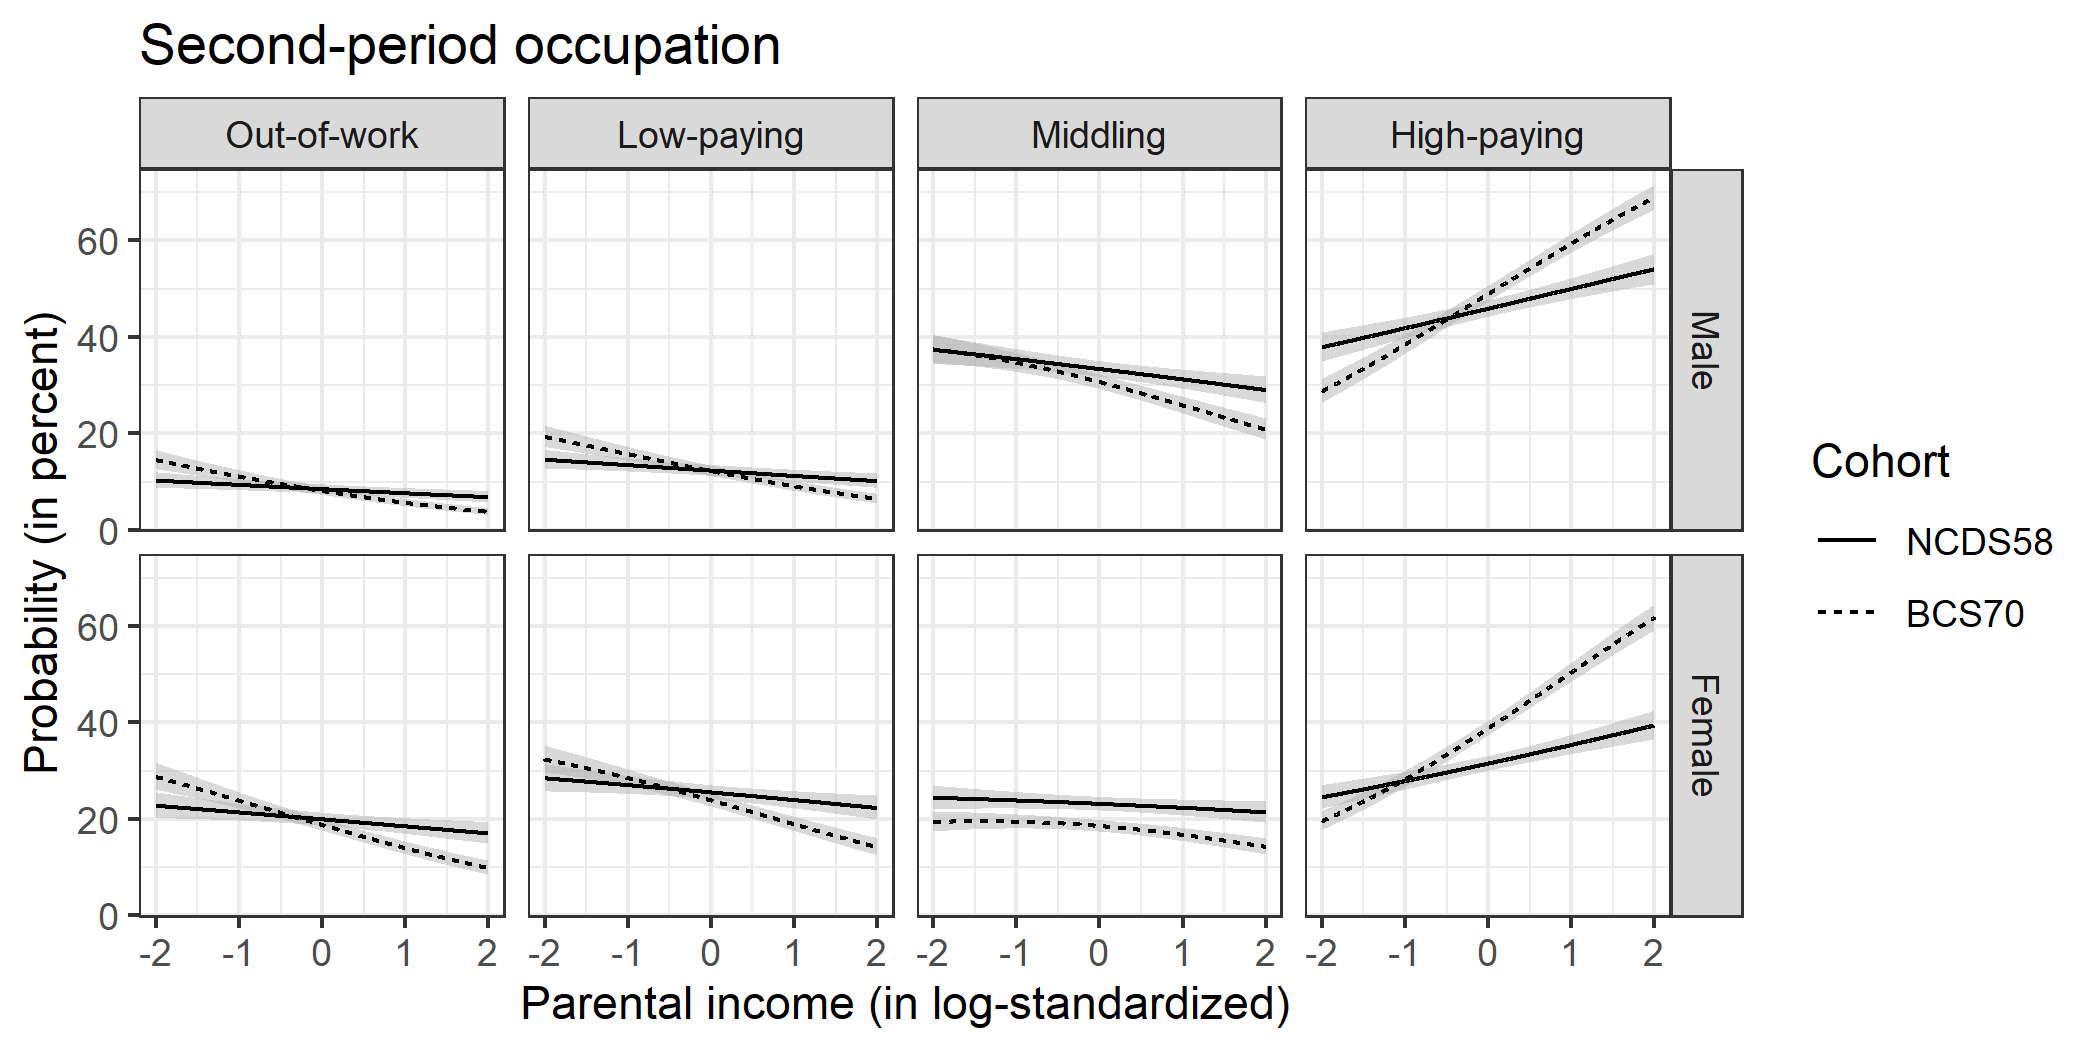
\includegraphics[width=\linewidth]{chap2/graphic/occ-multi2-pinc.png}
    \vspace{-3em}
	\justify\singlespacing\footnotesize{\textit{Notes:} This figure presents the probability, expressed in percent, of being in each type of occupation (out-of-work, low-paying, middling, high-paying) in second period according to parental income, in log-standardized.
	Probabilities are computed for males and females in both cohorts according to the multinomial logistic regression reported in Table \ref{chap2-tab:occ-multi23-base} in the appendix.}
\end{figure}
As for initial occupations, coming from a better-off background increases the probability of being in a high-paying occupation and reduces all others. The main difference with our results for initial occupations is the crossing of several of the probability schedules. Consider the probability of being in a high-paying occupation; we can ask whether individuals from all backgrounds have benefited from the increase in the share of such jobs across the two cohorts. Figure \ref{chap2-fig:occ-multi1-pinc} indicates that, as far as initial occupations are concerned, this is the case, with even those men at the bottom of the parental-income distribution (i.e. 2 standard deviations below the average) exhibiting a larger probability of being in a high-paying job for the younger than for the older cohort. In contrast, we can see in Figure \ref{chap2-fig:occ-multi2-pinc} that by age 42 only those from sufficiently well-off households have reaped the benefits of the expansion in high-paying jobs. Men whose parents had an income 0.5 standard-deviations below the average had the same probability of being in a high-paying occupation in both cohorts; those with lower parental income, experienced a lower probability if born in 1970 than if born in 1958.

Figure \ref{chap2-fig:occ-multi2-pinc} is reminiscent of the analysis in \cite{Major2018Social}, who show, using the same data, that the effect of parental income on the probabilities of being in the various quintiles of the income distribution has increased across the two cohorts (see \cite{Major2018Social}, Figures 0.1 and 0.2). Our results indicate, not surprisingly, that the occupational structure is behind the observed changes in income mobility and closely mimic their findings when we consider the probabilities of being in each of the four occupations for each decile in the parental-income distribution (see Figure \ref{chap2-fig:occ-multi2-quant-male} in Appendix \ref{chap2-app-additional}).


\subsection{From initial to mature occupations} \label{chap2-intra}

The marked change in the overall effect of parental income across the two generations can be due to changes in either how parental income impacts initial occupations or in its effect on mobility during the child's career, i.e. on intra-generational mobility. As we have seen above, the influence of parental background on the former has become stronger; we turn next to whether coming from a better-off background also changes the extent to which, given her initial occupation, an individual progresses over her career.

Table \ref{chap2-tab:occ-multi23-base} in Appendix \ref{chap2-app-logit} reports the multinomial results when we introduce initial occupations in the regressions for occupation at 42 and we provide a graphical analysis in Figure \ref{chap2-fig:occ-multi3-pinc-male}. The figure displays the difference, expressed in percentage points, in the probability of being in each second-period occupation (out-of-work, low-paying, middling, high-paying) conditional on first-period occupation between the BCS70 and the NCDS58 cohorts. 
\begin{figure}[!tb]
    \centering
    \caption{Change in second-period occupation probability conditional on first-period occupation and parental income (male only)}
    \label{chap2-fig:occ-multi3-pinc-male}
    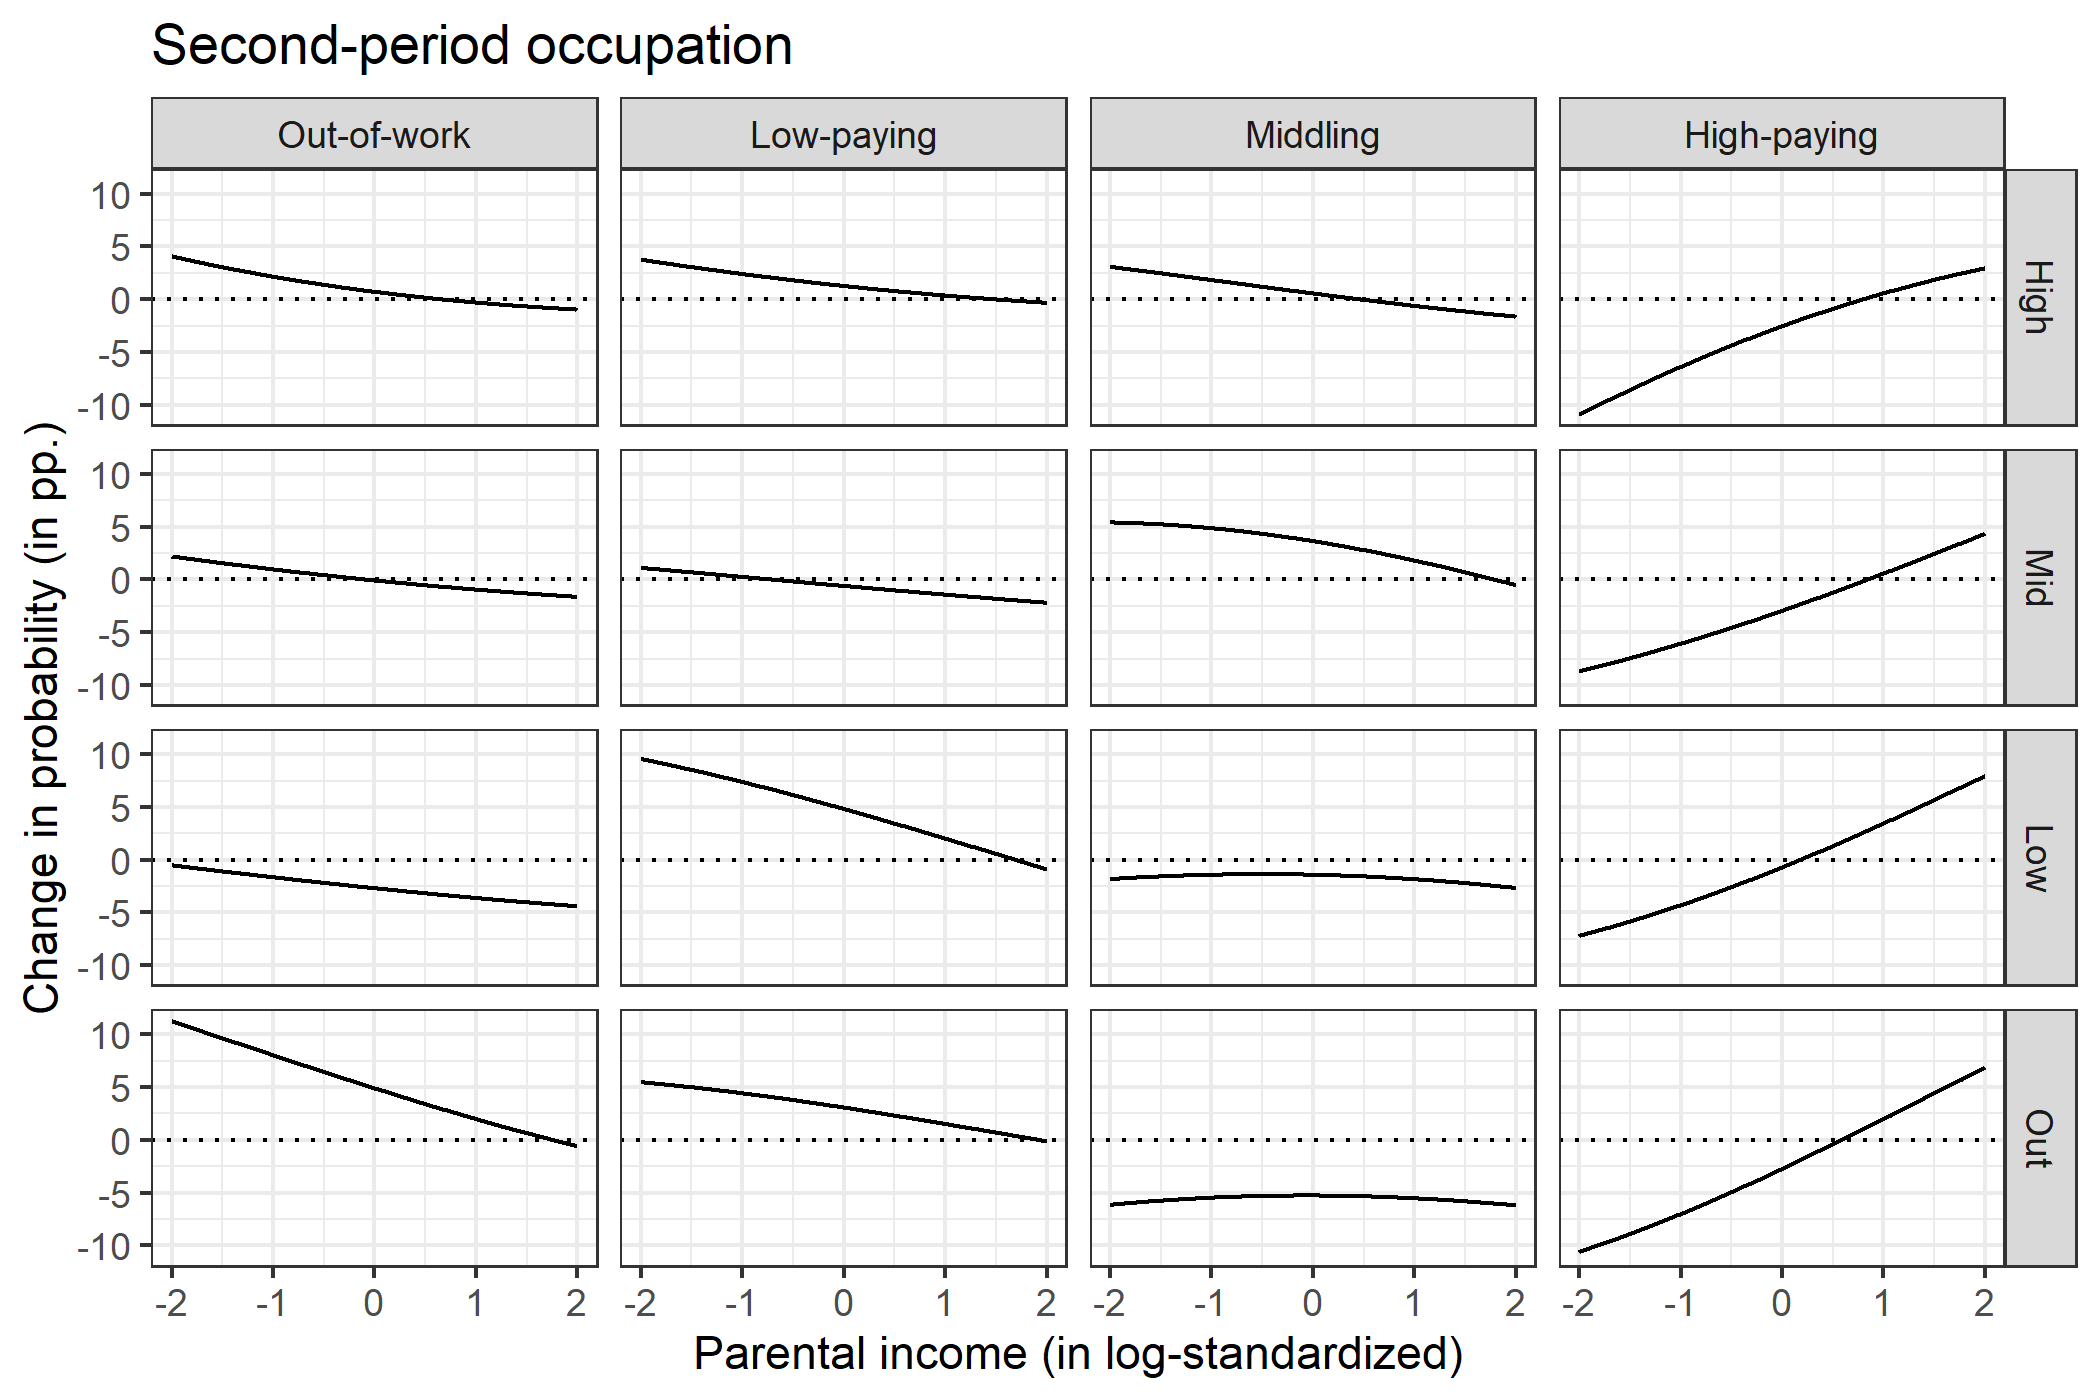
\includegraphics[width=\linewidth]{chap2/graphic/occ-multi3-pinc-male.png}
    \vspace{-3em}
    \justify\singlespacing\footnotesize{\textit{Notes:} This figure presents the difference, expressed in percentage points, between the BCS70 and the NCDS58 cohorts in terms of probability of being in each type of second-period occupation (out-of-work, low-paying, middling, high-paying), conditional on the first-period occupation, according to parental income, in log-standardized.
    Probabilities are computed for males in both cohorts according to the multinomial logistic regression reported in columns (2) of Table \ref{chap2-tab:occ-multi23-base}}
\end{figure}
Each panel represents the gap across cohorts in a particular transition probability for various levels of (standardized) parental income, with positive values implying that the younger cohort has a greater probability of moving from occupation $j$ to occupation $k$, and vice versa. The reported changes are those for men, with the equivalent figure for women provided in appendix \ref{chap2-app-additional}---see Figure \ref{chap2-fig:occ-multi3-pinc-female}.

Consider first individuals at the mean of the distribution. The probability of being in a middling occupation in late career has increased by almost 3.7 pp. for those who started in such occupation but declined for those starting in low-paying occupations or out of work. This indicates a reduction in upwards mobility for those starting in the least well-paid categories. For example, for those who were initially out-of-work, the probability of remaining there has increased by 4.92 pp., and although the probability of being in a high-paying occupation at 42 has slightly increased (by 0.71 pp.), this has occurred at the expense of a large decline in the likelihood of moving into low-paying or middling jobs. The fourth column of graphs, reporting changes in the probability of being in a high-paying occupation, indicates that---for those with mean parental income---the probability of being in such an occupation has fallen irrespective of the initial job. The change is small for those starting in low-paying occupations (-0.71 pp.) but larger for the other three initial occupations, with values between -2.5 and -2.9 pp. This is a surprising finding given that the share of such jobs rose by 5.4 pp.

These changes hide large differences depending on parental background. Consider the changes in the probability of being in a high-paying occupation across cohorts. For those at the top and the bottom of the parental income distribution the changes are large and of opposite sign. Notably, for those who came from a household with parental income 2-standard-deviations below the mean there is a reduction in the probability of attaining the top occupations, irrespective of the initial occupation, which is of considerable magnitude, between 7.2 and 11 pp.. Note that even those who started in high-paying occupations are now less likely to remain there if parental income is low. In contrast, when parental income is 2-standard-deviations above the mean, there is an increase in the likelihood of remaining in or moving to the top, with those who started in a low-paying occupation experiencing a particularly large increase, by 8 pp. 

The second important pattern observed in the data is a dichotomy that appears for those who started in a low-paying occupation. Their probability of moving to a middling occupation has fallen, but the alternative outcome depends on parental income. For those at the bottom of the distribution, the likelihood of remaining in a low-paying occupation has increased (by  4.8 pp. for those with average parental income and by 9.6 pp. for those at -2 standard deviations). In contrast, for those at the top of the parental income distribution the decline in mobility into middling jobs has been accompanied by a greater probability of moving into a high-paying occupation. The natural progression in which individuals would move from low-paying into middling occupations as their careers evolved seems to have weakened, and has been replaced by higher probabilities of either staying in the occupation of origin or jumping up to a high-paying one, with the transition probabilities being strongly dependent on parental income. An equivalent pattern is found when considering those who started in middling occupations, with those at the top (bottom) of the parental income distribution being more likely to be in high-paying (low-paying) jobs in the younger than in the older cohort. 

\subsection{Intra-generational mobility and parental income}

In order to provide a compact measure of mobility, we define three possible outcomes for the second period. Downward mobility is defined as ending up in a category with lower average pay than the individual's initial category; persistence consists of remaining in the same category, and upwards mobility occurs when the individual moves to a category with higher average pay. Hence for those starting in a low-paying occupation, downward mobility occurs if they are out-of-work at age 42, and upwards mobility if they are in a middling or high-paying occupation. 

The upwards/downwards intra-generational mobility measures are depicted graphically in Figure \ref{chap2-fig:persist-both}, in which we plot the \emph{change} in the three probabilities (of moving up, remaining in, and moving down with respect to the initial occupation) for different deciles of the parental income distribution; see also Table \ref{chap2-tab:mob-pinc-both} in the appendix.
\begin{figure}[!tb]
    \centering
    \caption{Change in intra-generational mobility across cohorts}
    \label{chap2-fig:persist-both}
    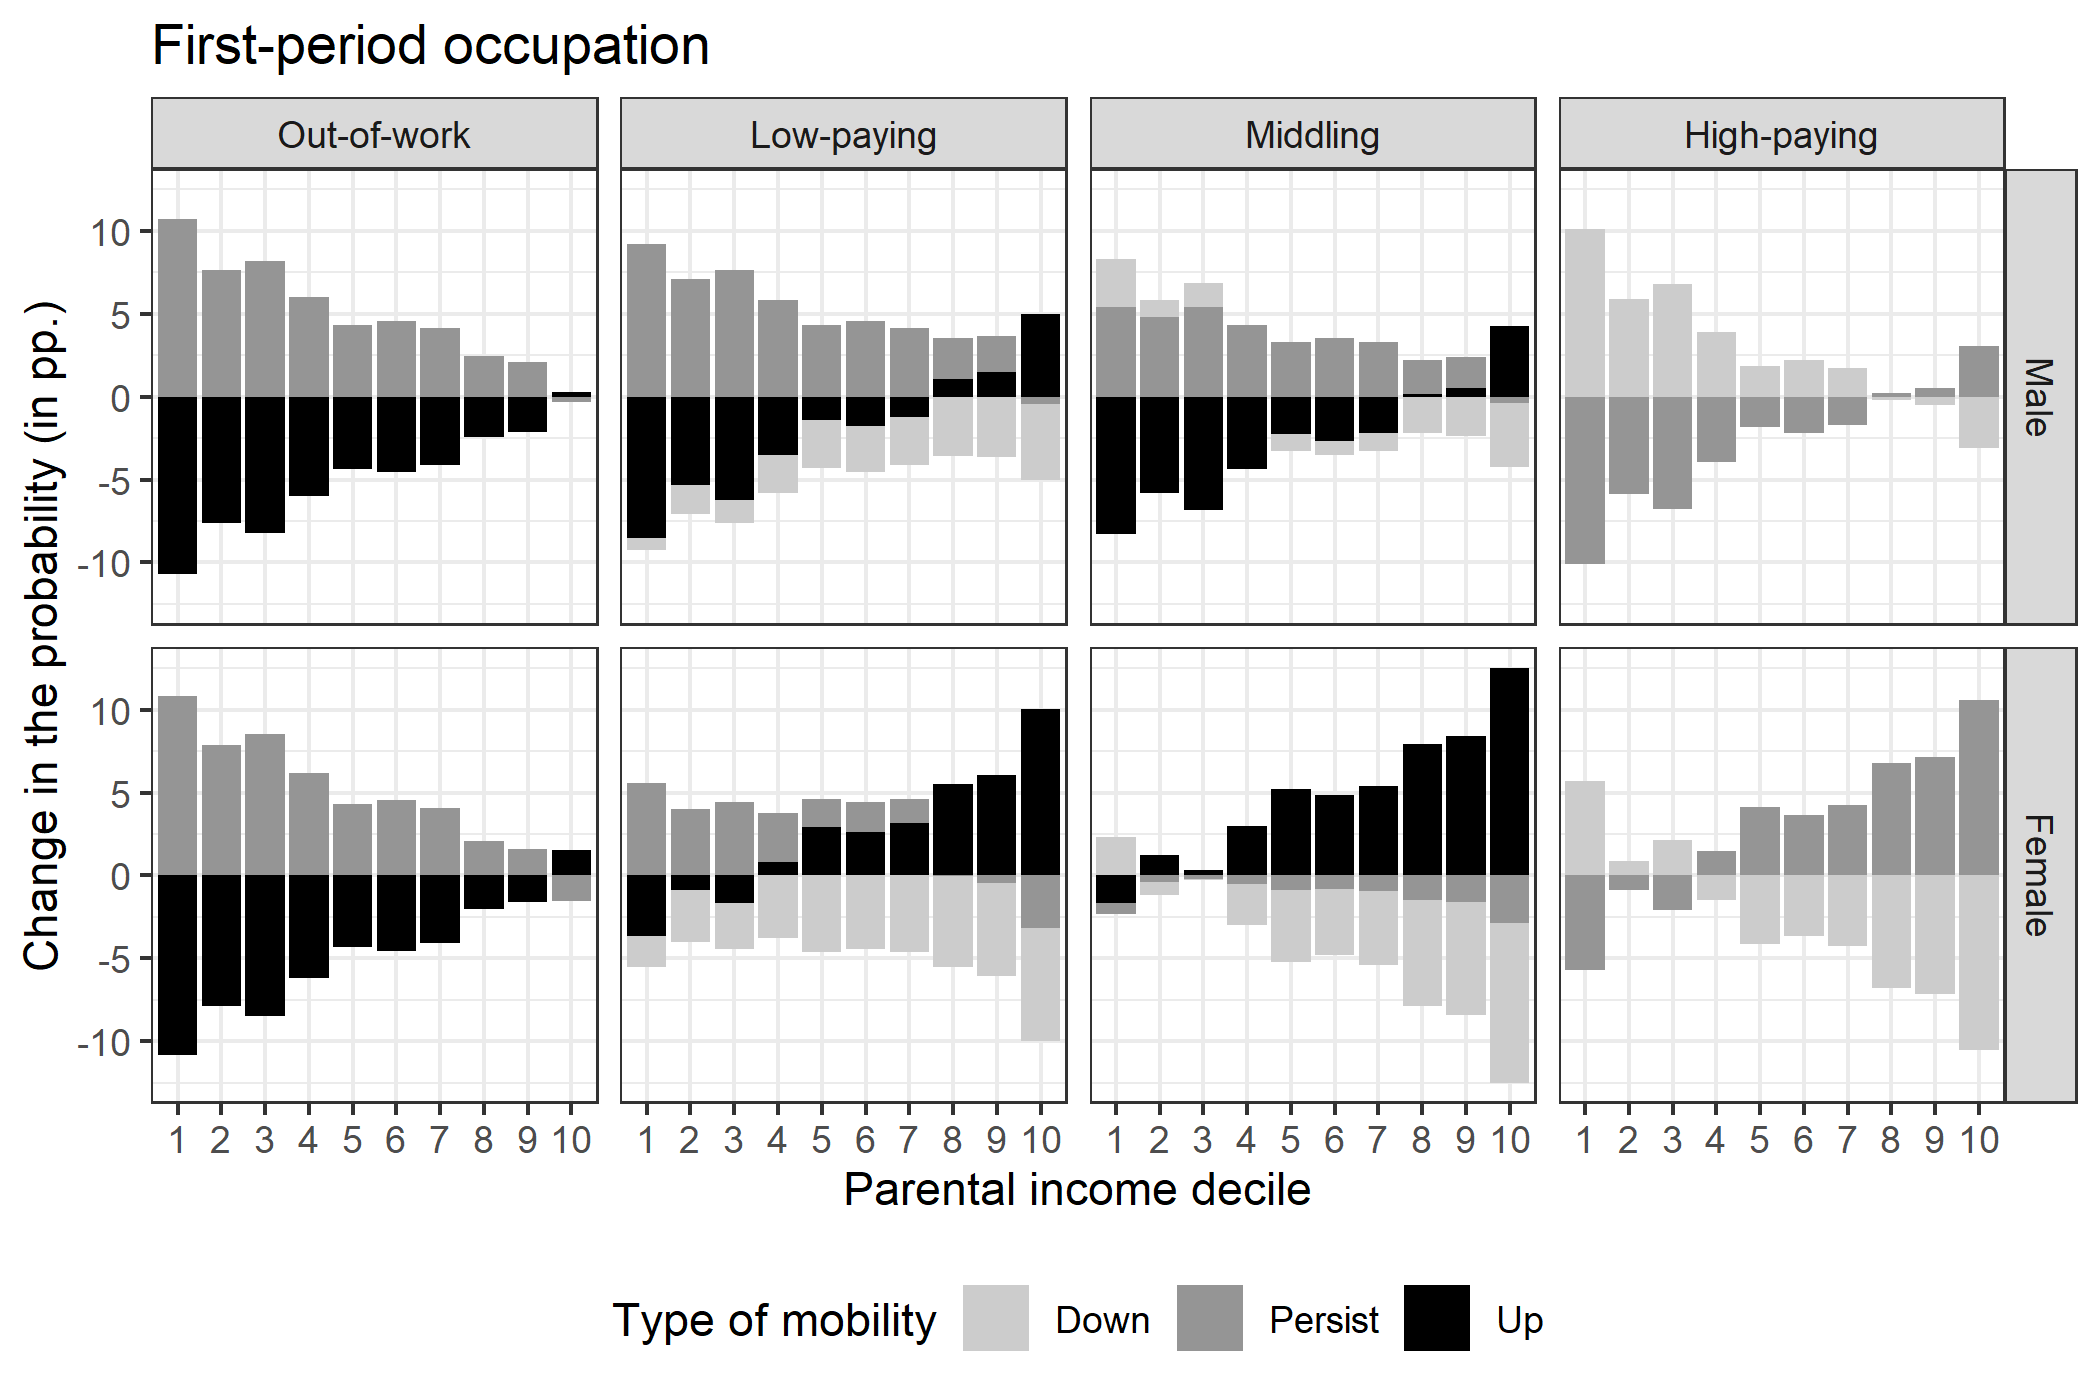
\includegraphics[width=\linewidth]{chap2/graphic/persist-both.png}
    \vspace{-3em}
    \justify\singlespacing\footnotesize{\textit{Notes:} This figure presents the difference, expressed in percentage points, between the BCS70 and the NCDS58 cohorts in terms of type of mobility (down, persist, up) conditional on the first period occupation (out-of-work, low-paying, middling, high-paying) according to the decile of the parental income distribution.
    Probabilities are computed for males and females at each parental income decile, according to the multinomial logistic regression reported in columns (2) of Table \ref{chap2-tab:occ-multi23-base} in the appendix.}
\end{figure}

Consider first those who started in high-paying occupations. The two possible occupational dynamics are to move downwards (depicted in light grey) or to remain in a high-paying occupation (depicted in dark grey). Those born to parents in the top decile are 3 pp. more likely to stay in that occupation and 3 pp. less likely to move into a lower-income occupation in the 1970 cohort than those born in 1958. The reverse effect appears for those at the bottom of the parental income distribution, with those in the bottom decile being 10 pp. more (less) likely to experience downwards mobility (remain in the occupation). The reduction in persistence falls as we move up the parental income distribution, with the sign reversing for the 9th and 10th deciles. The figure displays what we could call a \emph{polarization of mobility}, whereby for those in the middle of the distribution there have been only moderate changes in mobility, while at the extreme the changes have been large, although in opposite directions for those at the bottom and at the top. 

An equivalent pattern is observed for those that start their careers in middling occupations. Those at the bottom of the parental distribution witnessed sharp declines in upwards mobility and higher persistence and likelihood of moving down, with the size of the changes declining as we move along the income distribution. The pattern is reversed from the 8th decile, with the likelihood of moving upwards increasing across cohorts for the top three deciles. The polarization of mobility is also apparent for those starting in low-paying occupations for whom the probability of moving into middling or high-paying occupations increases only for the top three deciles. Lastly, for those initially out-of-work, only those in the top decile of the parental income distribution witness an increase in the likelihood of upwards mobility. Note that for those in the bottom decile the magnitudes of the change are large: the probability of staying has increased by 10 pp., which is offset by an equivalent decline in the probability of moving upwards. Overall these results indicate that the change in the structure of employment has been accompanied by a polarization of intra-generational mobility, with the probabilities of moving across occupations changing in opposite directions depending on whether individuals had parents at the top or at the bottom of the income distribution.

Not surprisingly, the dynamics for women differ considerably from those for men, as women of the older cohort where much less likely to occupy middling and especially high-paying occupations. The bottom panels of Figure \ref{chap2-fig:persist-both} capture, however, the advantage that parental income gives in providing the means for upwards mobility. Irrespective of parental income, women starting in a high-paying occupation (resp. middling) have a greater probability of remaining there (moving upwards) for the younger cohort. This is not surprising in view of the occupational upgrading experienced by women of the younger cohort. In contrast, for those who started in low-paying occupations, a polarization appears, although the turning point occurs for lower parental incomes than in the case of men (4th decile), indicating the tension between the general occupational upgrading of women and the decline in mobility observed for workers coming from a less well-off background. The results for those out of work broadly mimic those for men. Overall, despite the differences due to women's increased access to all occupations, these figures confirm the increased importance of parental income for intra-generational mobility.


    
    \section{Mobility and polarization at the regional level}\label{chap2-regional}
    \subsection{Regional polarization}

The geography of mobility has received considerable attention over the past few years,\footnote{See \cite{Chetty2014Land} and \cite{Bell2018Land} amongst others.} and in this section we turn to exploring the regional dimension of our data. We focus on two aspects, both of which address the hypothesis that the observed increase in the impact of parental income on occupational outcomes is related to the polarization of employment. The next subsection considers whether the reduction in mobility that we have identified appears when we replace the cohort dummies by a measure of the extent of polarization that individuals faced in their region when they were young. It hence asks if the cohort dummies are capturing the differences in the structure of the labour market over time. Our second strategy consists in estimating the impact of parental income on occupational outcomes at the regional level in order to get regional measures of mobility. We then ask whether there is a correlation between the changes over time in regional mobility and the increase in polarization at the local level.

Our data have information on 10 regions and hence do not allow us to identity the very local effects that other work has observed.\footnote{\cite{Chetty2014Land} focus on considerably smaller locations in their analysis for the US. For the UK, \cite{Bell2018Land} consider a dataset with the 32 NUTS2 regions but which does not have information on parental income.} For both analyses we need to construct a measure of polarization at the regional level, but we are impaired by the fact that sample sizes at the regional level are small and thus measures of regional polarization based on our cohort data may not capture well the actual changes in the structure of employment. In order to have a more representative sample we use data from the Labour Force Survey (LFS) to build polarization measures. 

When computing the extent of polarization we face two concerns. First, as shown in the appendix, the share of middling employment has fallen in all regions, but whether this has occurred at the expense of low-paying or high-paying occupations varies. For this reason, rather than focusing exclusively on the share of middling jobs we consider changes in the share of jobs in all three occupations. Second, we need to define the job market that individuals in our dataset were facing and measure the extent of polarization in that particular market. To do so we consider the distribution of employment for the relevant age cohorts in the LFS. We hence suppose that members of a cohort are in competition for jobs with individuals that were born in the 5 years before and 5 years after them. That is, for the NCDS58 cohort we consider individuals born between 1953 and 1963, and for the BCS70 those born between 1965 and 1975. We measure the share of employment in each year between the initial and final period that we use for each cohort, and compute the average over the whole period in which each cohort has been exposed to employment changes. That is, for the NCD58 we consider the structure of employment between 1981 and 2000, for the BCS70 between 1996 and 2012. We then measure the extent of polarization as changes in the occupational shares obtained for the 1953-63 cohorts and those for the 1965-75 ones. Appendix \ref{chap2-app-data-LFS} gives details on the LFS data and our measures of polarization, and shows that all regions exhibited an increase in polarization (see Figure \ref{chap2-fig:lfs-change}).


\subsection{Individual outcomes and regional employment patterns}

Several factors may be behind the increased importance of parental income for occupational outcomes across cohorts. Here we explore the possibility that employment polarization is one of these factors. To do so, we substitute the cohort dummy used in our regressions by our measure of regional polarization. We use the region in which the individual lived at age 16, and measure polarization in that region as the share of middling employment in the year in which the individuals are 23/26.

Table \ref{chap2-tab:regocc-multi2A-short} displays the results obtained from the multinomial regression, regression, with the first three columns reporting again the estimates when we use the cohort dummies (i.e. those in Table \ref{chap2-tab:occ-multi2-short} above), and the last three columns those in which we substitute the dummies for the share of non-middling jobs and this share interacted with parental income (both standardized). The regressions also include a region fixed effect. We focus on the effect of the share of non-middling employment as an increase in its value can be interpreted as an increase in polarization. \footnote{Results using jointly the low- and high-paying employment shares are reported in Table \ref{chap2-tab:regocc-multi2B-short} in the appendix. We also used alternative measures of polarization using data on only the initial year measure of polarization for each cohort (1981 and 1996) rather than the average over the working-life and found equivalent results to those reported here (results not reported).} 
\begin{table}[!tb]
    \centering
    \caption{Second-period occupation probability according to share of non-middling occupations in the region at the age 16}
    \label{chap2-tab:regocc-multi2A-short}
    \resizebox*{\textwidth}{!}{
    \begin{threeparttable}
        \setlength{\tabcolsep}{0pt}
        \begin{tabular}{l D{.}{.}{5.3} D{.}{.}{5.5} D{.}{.}{5.5} D{.}{.}{5.3} D{.}{.}{5.5} D{.}{.}{5.5}}
\toprule
 & \multicolumn{6}{c}{Multinomial logit - Dep. var.: Second-period occupation} \\
\cmidrule(lr){2-7}
 & \multicolumn{3}{c}{(1)} & \multicolumn{3}{c}{(2)} \\
\cmidrule(lr){2-4}\cmidrule(lr){5-7}
 & \multicolumn{1}{c}{Low} & \multicolumn{1}{c}{Mid} & \multicolumn{1}{c}{High} & \multicolumn{1}{c}{Low} & \multicolumn{1}{c}{Mid} & \multicolumn{1}{c}{High} \\
\midrule
BCS cohort                        & 0.05   & -0.03      & 0.11       &        &            &            \\
                                  & (0.11) & (0.09)     & (0.09)     &        &            &            \\
Non-Middling share                &        &            &            & 0.07   & 0.02       & 0.17^{***} \\
                                  &        &            &            & (0.06) & (0.05)     & (0.05)     \\
Parental income                   & 0.01   & 0.04       & 0.19^{***} & 0.04   & 0.11^{***} & 0.35^{***} \\
                                  & (0.04) & (0.04)     & (0.04)     & (0.03) & (0.03)     & (0.03)     \\
Par. inc. $\times$ BCS            & 0.05   & 0.16^{***} & 0.36^{***} &        &            &            \\
                                  & (0.06) & (0.05)     & (0.05)     &        &            &            \\
Par. inc. $\times$ Non-Mid. share &        &            &            & -0.00  & 0.04^{*}   & 0.11^{***} \\
                                  &        &            &            & (0.03) & (0.02)     & (0.02)     \\
\midrule
Num. obs. & \multicolumn{1}{c}{14763} & \multicolumn{1}{c}{14763} & \multicolumn{1}{c}{14763} & \multicolumn{1}{c}{14763} & \multicolumn{1}{c}{14763} & \multicolumn{1}{c}{14763}\\
\bottomrule
\end{tabular}

        \begin{tablenotes}[flushleft]
            \footnotesize{\item\textit{Notes}: 
            % Stars and SE
            $^{***}p<0.01$; $^{**}p<0.05$; $^{*}p<0.1$. Standard errors between parentheses. 
            % Baseline outcome
            Out-of-work occupation in second period is the base outcome of the multinomial logistic regression.
            % Referent group
            Male in the NCDS58 cohort is the referent group in (1), while male is the referent group in (2).
            % Variables details
            Parental income in logarithm and then standardized at the cohort level. 
            Non-middling share corresponds to the share of occupations that are not middling, hence, low-paying and high-paying, in total employment in the region at age 16. The shares has been standardized for the interpretability of coefficients when interacted with parental income.
            % Control variables
            Control variables in (1) include Intercept, Female and Female $\times$ BCS, while control variables in (2) include Intercept, Female and Female $\times$ Non-Mid. share. %; see Table \ref{chap2-tab:tobefilled} in the appendix for these coefficients.
            }
        \end{tablenotes}
    \end{threeparttable}
    }
\end{table}

The coefficients of interest have the expected sign. A higher share of non-middling employment is associated with a greater average probability of being in a high-paying occupation, as we would expect given the greater availability of these jobs. There is no significant effect on the other employment categories, implying that higher polarization does not affect the allocation of workers between out-of-work, low-paying jobs and middling jobs. Parental income has, as expected, a positive impact on the likelihood to be in middling and high-paying jobs, and the interaction terms indicate that as polarization increases the effect of background becomes stronger. To gauge the magnitude of these effects, we average the (standardized) share of middling employment across regions for each cohort, obtaining that for the NCDS58 (resp. BCS70) it is 0.845 standard deviations below (above) the mean. Using these figures, the coefficients on column (6) imply that a one standard deviation increase in parental income raised the probability of being in a high-paying occupation by 0.14 pp. for the older cohort and by 0.44 for the younger one. These values are close to those obtained in our core specification (column (3)) of 0.19 and 0.55, indicating that using the differences in polarization across cohorts yield effects that are close to those obtained with the cohort dummy. 


\subsection{Regional mobility} 

Our final step consists in exploiting the cross-sectional variation in the regional data to consider the correlation between regional mobility and polarization. We start by running the same multinomial regressions as in equation \ref{chap2-eq:emp-multi3} but at the regional level.\footnote{We do not compute first-period mobility and conditional second-period mobility because of sample sizes, as in many regions we have only a small number of individuals moving across certain occupations between first and second period.} Table \ref{chap2-tab:reg-multi2-short} presents the coefficients on parental income obtained when we regress second period occupation on parental income. As before, we need to recall that these are the coefficients relative to the probability of being out-of-work (see also Figures \ref{chap2-fig:reg-multi2-pinc-male} and \ref{chap2-fig:reg-multi2-pinc-female} in the appendix).

\begin{table}[!tb]
    \centering
    \caption{Probability of second-period occupation by region}
    \label{chap2-tab:reg-multi2-short}
    \resizebox*{!}{\dimexpr\textheight-2\baselineskip\relax}{
    \begin{threeparttable}
        \centering
        \setlength{\tabcolsep}{12pt}
        \begin{tabular}{l D{.}{.}{3.5} D{.}{.}{3.5} D{.}{.}{3.5}}
\toprule
 & \multicolumn{3}{c}{Multi. logit - Dep. var.: Second-period occupation} \\
\cmidrule(lr){2-4}
 & \multicolumn{1}{c}{Low-paying} & \multicolumn{1}{c}{Middling} & \multicolumn{1}{c}{High-paying} \\
\midrule
\midrule
 East Anglia (N = 904) & & & \\
\midrule
Par. inc.              & 0.04       & -0.00       & 0.13        \\
                       & (0.15)     & (0.14)      & (0.14)      \\
Par. inc. $\times$ BCS & -0.10      & 0.31        & 0.57^{**}   \\
                       & (0.25)     & (0.26)      & (0.26)      \\
\midrule
 East Midlands (N = 1066) & & & \\
\midrule
Par. inc.              & 0.06       & 0.12        & 0.17        \\
                       & (0.15)     & (0.15)      & (0.15)      \\
Par. inc. $\times$ BCS & 0.45^{**}  & 0.44^{**}   & 0.92^{***}  \\
                       & (0.22)     & (0.21)      & (0.21)      \\
\midrule
 North (N = 1037) & & & \\
\midrule
Par. inc.              & -0.04  & -0.08       & 0.02        \\
                       & (0.15) & (0.14)      & (0.14)      \\
Par. inc. $\times$ BCS & 0.07   & 0.34        & 0.58^{***}  \\
                       & (0.22) & (0.22)      & (0.21)      \\
\midrule
 North West (N = 1810) & & & \\
\midrule
Par. inc.              & 0.12       & 0.06        & 0.32^{***}  \\
                       & (0.11)     & (0.10)      & (0.11)      \\
Par. inc. $\times$ BCS & -0.01      & 0.32^{**}   & 0.35^{**}   \\
                       & (0.16)     & (0.15)      & (0.15)      \\
\midrule
 Scotland (N = 1489) & & & \\
\midrule
Par. inc.              & 0.03   & 0.13        & 0.14        \\
                       & (0.12) & (0.12)      & (0.12)      \\
Par. inc. $\times$ BCS & 0.18   & 0.17        & 0.52^{***}  \\
                       & (0.18) & (0.18)      & (0.17)      \\
\midrule
 South East (N = 3718) & & & \\
\midrule
Par. inc.              & 0.01       & 0.06        & 0.17^{**}   \\
                       & (0.09)     & (0.08)      & (0.08)      \\
Par. inc. $\times$ BCS & -0.06      & 0.02        & 0.26^{**}   \\
                       & (0.11)     & (0.11)      & (0.11)      \\
\midrule
 South West (N = 1141) & & & \\
\midrule
Par. inc.              & -0.10      & 0.05        & 0.17        \\
                       & (0.16)     & (0.16)      & (0.16)      \\
Par. inc. $\times$ BCS & 0.08       & -0.02       & 0.31        \\
                       & (0.21)     & (0.21)      & (0.21)      \\
\midrule
 Wales (N = 821) & & & \\
\midrule
Par. inc.              & -0.23  & -0.16       & -0.07      \\
                       & (0.17) & (0.16)      & (0.16)     \\
Par. inc. $\times$ BCS & 0.34   & 0.27        & 0.62^{***} \\
                       & (0.24) & (0.23)      & (0.22)     \\
\midrule
 West Midlands (N = 1495) & & & \\
\midrule
Par. inc.              & 0.04   & 0.12        & 0.63^{***}  \\
                       & (0.12) & (0.12)      & (0.14)      \\
Par. inc. $\times$ BCS & 0.09   & 0.12        & -0.08       \\
                       & (0.17) & (0.17)      & (0.18)      \\
\midrule
 Yorkshire and Humberside (N = 1282) & & & \\
\midrule
Par. inc.              & 0.03   & -0.05       & 0.02        \\
                       & (0.14) & (0.12)      & (0.12)      \\
Par. inc. $\times$ BCS & 0.06   & 0.21        & 0.53^{***}  \\
                       & (0.19) & (0.17)      & (0.17)      \\
\bottomrule
\end{tabular}

        \begin{tablenotes}[flushleft]
            \footnotesize{\item \textit{Notes}: 
            % Stars and SE
            $^{***}p<0.01$; $^{**}p<0.05$; $^{*}p<0.1$. Standard errors between parentheses. 
            % Baseline outcome
            Out-of-work occupation in second period is the base outcome of the multinomial logistic regression.
            % Referent group
            Male in the NCDS58 cohort is the referent group.
            % Variables details
            Parental income in logarithm and then standardized at the cohort level.
            % Control variables
            Control variables in all regressions include Intercept, BCS cohort, Female and Female $\times$ BCS.}
        \end{tablenotes}
    \end{threeparttable}
    }
\end{table}

These regressions allow us to make two inferences. First, we can ask whether the changes in occupational mobility observed across cohorts at the national level also took place at the regional level and are not the result of the population reallocating across regions with different mobility patterns. When we split the data we find that for the vast majority of regions (7/10) parental income exhibits insignificant coefficients for the older cohort. Only in the North West, the South East and the West Midlands do we find a significant coefficient on parental income. Note, however, that out of the seven regions for which the coefficient is not significant, 4 of them have magnitudes close to the 0.19 point estimate we obtained at the national level. The lack of significance can then be due to a lack of statistical power given the limited number of observations (per region and also in certain region-occupation cells). For those born in 1970, the likelihood to be in a high-paying occupation exhibits systematically large and significant coefficients on parental income. Out of the 10 regions only two (South West and West Midlands) do not display a significant coefficient. In all the others, the magnitude of the effect is large, with the coefficient being at least twice as large for the younger as for the older cohort (eg. North West) and much larger in others. These results indicate that the increase in the importance of parental income across cohorts holds at the regional level.

Second, the estimates imply large variations in the degree of inter-generational income mobility across locations, with the probability of someone born in a household in the bottom quintile moving to the top quintile being three times higher in the most than in the least mobile locations. This raises the question of whether the magnitude of the changes in mobility is correlated to the degree of employment polarization observed at the regional level. 

To capture changes in mobility in region $r$, we consider the between-cohort change in the role of parental income for being in a high-paying occupation, namely, $\Delta\beta_H^r$. These coefficients correspond to the ``$\text{Par. Inc. }\times\text{ BCS}$'' coefficients in Table \ref{chap2-tab:reg-multi2-short}. The change in the extent of regional polarization is measured by the change across cohorts in regional polarization as measured from the LFS. Figure \ref{chap2-fig:regocc-absolute-high} displays the correlation between the two variables, with both measured in percentage points. The three panels report, in the horizontal axis, the changes in absolute value of the share of employment in each of the three categories. The actual changes are positive for high- and low-paying occupations and negative for middling ones, hence reporting the absolute value implies that for all three occupational categories moving from the left to the right of each graph implies an increase in polarization. The vertical axis displays the regional $\Delta\beta_{H}$ described above.
\begin{figure}[!tb]
    \centering
    \caption{Change in parental income coefficient for high-paying second-period occupation according to job polarization at the regional level}
    \label{chap2-fig:regocc-absolute-high}
    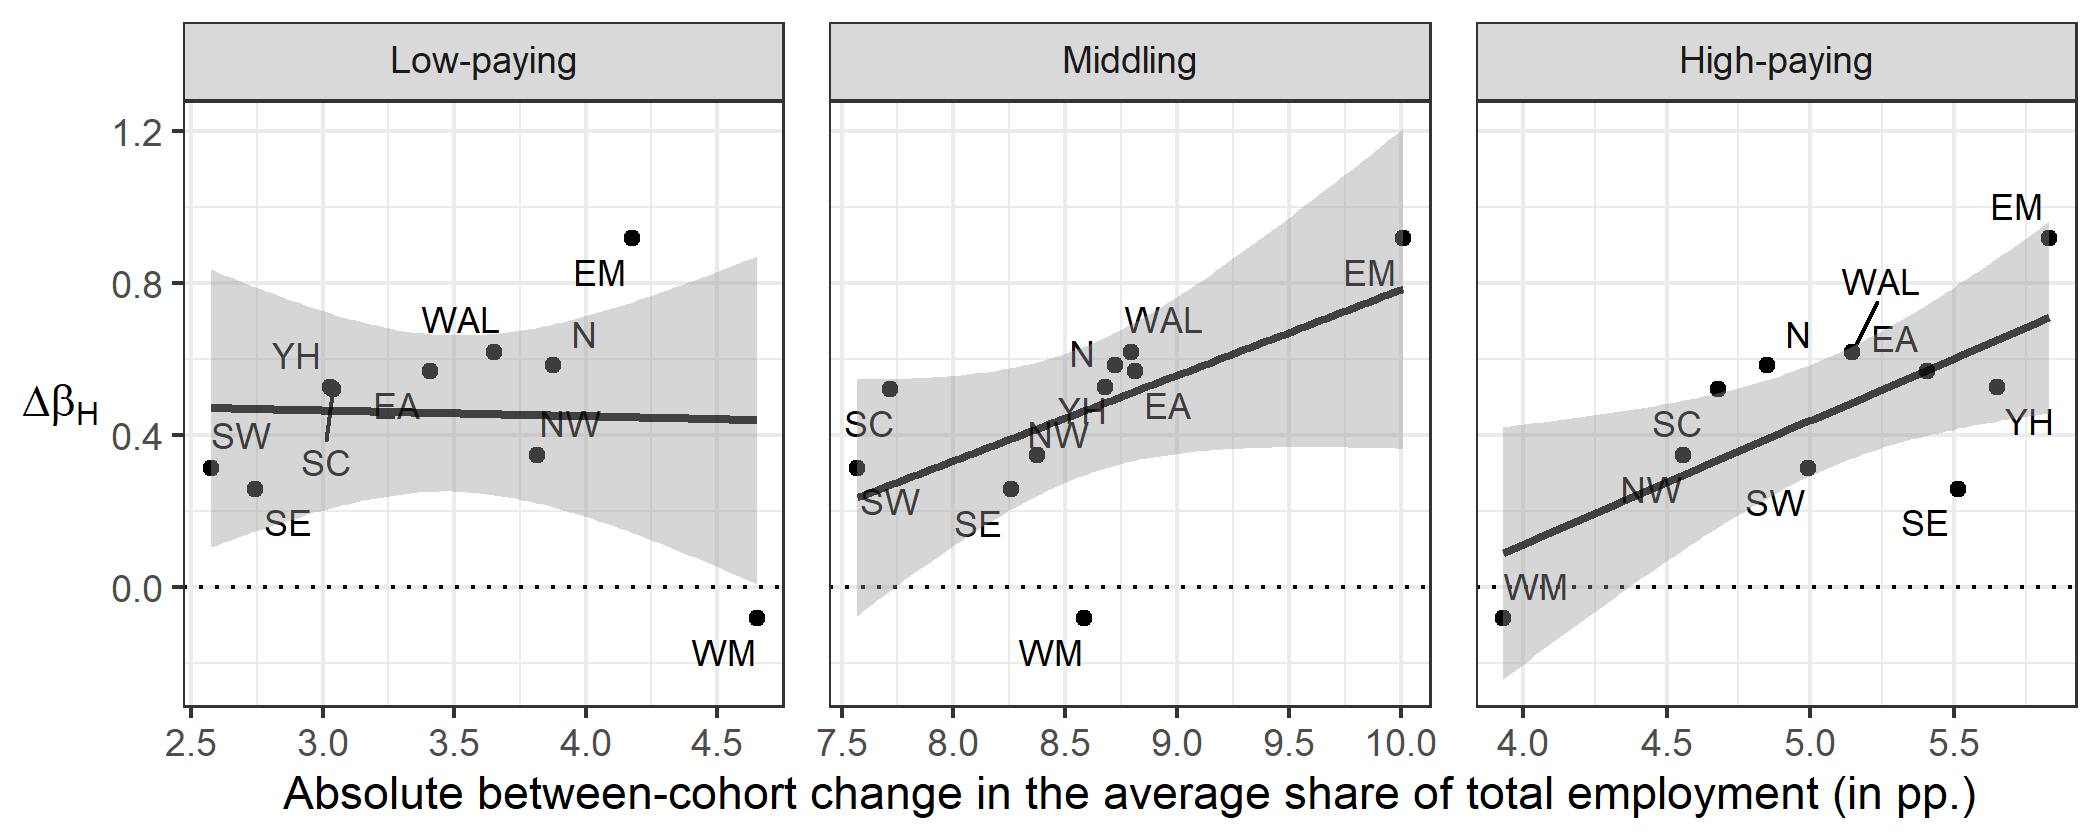
\includegraphics[width=\linewidth]{chap2/graphic/regocc-absolute-high.png}
    \vspace{-3em}
	\justify\singlespacing\footnotesize{\textit{Notes:} This figure presents the correlation across regions between the change in the parental income coefficient for the high-paying occupation in second period $\Delta\beta_H$ and the between-cohort change in absolute value in the average share of total employment of low-paying, middling, and high-paying occupations, in percentage points. Note that, by taking the absolute value of the change, we reversed the x-axis for the middling panels (middle column). Thus, regions on the left-hand (resp. right-hand) side of each panel are those where the polarization of employment has been lower (resp. larger).}
\end{figure}

Each dot represents one of the 10 regions, while the line corresponds to the linear regression line.\footnote{Figure \ref{chap2-fig:regocc-absolute-all} in the appendix presents equivalent graphs for the change in the coefficients on parental income in the probability of being in middling and low-paying occupations, namely, $\Delta\beta_{M}$ and $\Delta\beta_{L}$. We obtain broadly similar results in the two cases,} Consider the right-most graph. The upward slope indicates that regions where the share of high-paying occupations (in the relevant age group) increased the most are also the regions where the impact of parental income in accessing high-paying occupations rose the most. Similarly, the middle graph also displays an upwards-slopping schedule when we plot the magnitude of the change in the share of middling occupations against $\Delta\beta_{H}$, indicating that regions where the share of middling income jobs declined the most are also those where parental impact became strongest. The left-hand graph depicts the correlation between the change in the coefficient and the change in the share of low-paying occupations, and displays a flat schedule, which is driven by an outlier, the West-Midlands. Removing this observation, yields a positive correlation between the change in polarization and the change in the effect of parental income.

This subsection, together with the previous one, provide suggestive evidence that the increase in employment polarization may be a cause of the reduction in occupational mobility observed across the two cohorts. When we exploit the time dimension, we find that differences in the extent of polarization experienced by the two cohorts result in estimates of the impact of parental income that are close to those obtained when using cohort dummies. The cross-sectional evidence, in turn, indicates that when we estimate mobility measures by regions, the increases in \emph{immobility} that we observe are correlated with regional increases in polarization.





    
    \section{Conclusion} \label{chap2-conclusion}
    A vast literature has discussed the consequences of job polarization for wage inequality. In contrast, little is known about whether the change in the employment structure has also had an impact on social mobility. This paper raises such question using British data for two cohorts for which we have information for parents and children.

We start by developing a simple theoretical setup with three types of jobs and two levels of parental income. Parental background will affect the child's human capital so that the latter’s productivity is determined both by human capital and innate (and initially unobservable) ability. Children’s entry jobs will be determined by parental background, but as their ability is revealed, they may move up or down the occupational ladder. As the share of middle jobs disappears, the possibilities for mobility fall, thus leading to greater job persistence across generations.

The model highlights not only the importance of polarization for social mobility, but also the fact that transitions across occupations---i.e. intra-generational occupational dynamics---are an essential aspect of inter-generational mobility. Our empirical approach uses data on two British cohorts that are particularly suited for our purposes. First, the two cohorts, born 12  years apart, entered the labour market under substantially different conditions in terms of the structure of employment, with the latter cohort facing a much more polarized labour market. Second, we have data for children at various ages so that we can identify to what extent upwards mobility is driven by an improvement in the occupation at which children enter the labour market or by them going up the occupational ladder during their work-life. 

The data indicate that intra-generational occupational changes are an important source of mobility, with large shares of those starting in low-paying and middling occupations moving, respectively, to middling and high-paying jobs over their work lives. When we compare the two cohorts, we find that as the share of middling jobs has fallen these two sources of occupational mobility have weakened. Our results indicate that the role of parental income in determining occupations has increased, both for first-period occupations and for the transition towards better-paid occupations. For example, the fortunes of those who start in low-paying jobs differ considerably across generations. For the older cohort, a considerable fraction moved into middling jobs, but this probability has fallen markedly for the younger cohort. At the same time, the probability for those who start in low-paying jobs to move into high-paying jobs has remained roughly stable on average, but this average hides the fact that it has considerably increased for those with high-income parents and declined for those from low-income backgrounds. 

Although our data does not allow us to establish causality, the changes we identify are suggestive that as middling jobs have been eroded, parental income has become more important in determining occupational outcomes. Our analysis of regional mobility patterns finds that regions where employment polarization rose the most are also those where \emph{immobility} increased the most. These results hence suggest that the structure of employment affects not only the distribution of earnings but also the degree of occupational mobility. Moreover, they point towards the possibility that there is a transmission of polarization across generations, and that the increased importance of parental background may accumulate across generations creating a multiplier effect that over time accentuates the occupational distance across groups from different backgrounds. This is a question that we intend to pursue in future work. 
    
    \printbibliography[heading=subbibintoc]
    
    \clearpage
    \addsec{Appendices}
    \renewcommand{\thesubsection}{\thechapter.\Alph{subsection}}
    
    \subsection{Model derivations}\label{chap2-app-model}
    This appendix presents details on the model.

\subsubsection{The allocation of labour under imperfect information}

Under imperfect information, the second-period distribution of expected skills is given by
\begin{equation*}
    h=\left\{ 
    \begin{array}{cc}
    \underline{h}_{L} & (1-\pi )(z_{L}-q_1) \\ 
    \widehat{h}_L & q_{1} \\ 
    \underline{h}_{H} & (1-\pi )z_{H} \\ 
    \overline{h}_{L} & \pi (z_{L}-q_1) \\ 
    \overline{h}_{H} & \pi z_{H}%
    \end{array}%
    \right.  
\end{equation*}

Let $d_{1,2}$ (resp. $d_{2,3}$) be the threshold productivity between low-paying and middling jobs (resp. middling and high-paying jobs), i.e. $d_{1,2}$ is the skill for which individuals below this level are assigned to job type $1$. By construction, we have that $d_{1,2} \leq d_{2,3}$. Various scenarii are possible, and we focus on the case where low-paying jobs are filled with individuals from low-skill households, while middling and high-paying jobs contain workers from both low- and high-skill households. Assumption \ref{chap2-ass:threshold-skill-p2} ensures that this is the case. 

Under assumptions \ref{chap2-ass:threshold-skill-p1} and \ref{chap2-ass:threshold-skill-p2}, the
probability that an individual with parental background $i=\{L,H\}$ is in occupation $k\in\{1,2,3\}$ when mature, namely $P_j(k)$, is given by
\begin{align*}
    P_L(1) &=\frac{q_1}{z_L}, &&P_H(1) = 0,\\
    P_L(2) &=(1-\pi)\left(1-\frac{q_1}{z_L}\right), &&P_H(2) = 1- \pi - \frac{q_{3}-\pi (1-q_{1})}{z_{H}},\\
    P_L(3) &=\pi \left(1-\frac{q_1}{z_L}\right), &&P_H(3) = \pi +\frac{q_{3}-\pi (1-q_{1})}{z_{H}}.
\end{align*}
Note that Assumption \ref{chap2-ass:threshold-skill-p2} above imply that $q_{3}-\pi (1-q_{1})>0$. 

We can now consider how changes in $q_{1}$ and $q_{3}$ (at the expense of $q_{2}$) affect inter-generational mobility. As long as Assumptions \ref{chap2-ass:threshold-skill-p1} and \ref{chap2-ass:threshold-skill-p2} hold, we have that
\begin{itemize}
    \item An increase in $q_{1}$ increases the probability of being in occupation 1 and reduces those of being in occupations 2 and 3 for individuals from low-income households. For individuals from high-income households, it increases the probability of being in occupation 3 and reduces that of being in occupation 2.
    \item An increase in $q_{3}$ has no effect on the probabilities for individuals from low-skilled households. For individuals from high-income households, it increases the probability of being in occupation 3 and reduces that of being in occupation 2.
\end{itemize}

\subsubsection{The occupation distribution of mature workers under perfect information }

In this subsection we consider the way in which our assumption about the information content of occupations affects mobility. We compare the distribution of occupations obtained under this assumption with that in the case in which there is perfect information. Under perfect information, firms face a distribution of skills in which they know for all workers whether they are high or low ability as well as their family type. The distribution of observed second-period skills is then
\begin{equation*}
    h=\left\{ 
    \begin{array}{cc}
        \underline{h}_{L} & (1-\pi )z_{L} \\ 
        \underline{h}_{H} & (1-\pi )z_{H} \\ 
        \overline{h}_{L} & \pi z_{L} \\ 
        \overline{h}_{H} & \pi z_{H}%
    \end{array}%
    \right.  
\end{equation*}

Under assumptions \ref{chap2-ass:threshold-skill-p1} and \ref{chap2-ass:threshold-skill-p2}, the
probability that an individual with parental background $i=\{L,H\}$ is in occupation $k\in\{1,2,3\}$ when mature, namely $P^\prime_i(k)$, is given by
\begin{align*}
    P^\prime_L(1) &=\frac{q_1}{z_L}, &&P^\prime_H(1) = 0,\\
    P^\prime_L(2) &=1-\frac{q_1+q_3}{z_{L}}, &&P^\prime_H(2) = 1-\pi,\\
    P^\prime_L(3) &=\frac{q_{3}-\pi (1-z_{L})}{z_{L}}, &&P^\prime_H(3) = \pi.
\end{align*}
These expressions imply that for those born in high-income households, the probabilities of being in the various occupations are independent of the distribution of employment. For those born in low-income households, both $q_1$ and $q_3$ have an impact. An increase in either of them (i.e. greater polarization) would reduce the share of those born in low-income households that works in middling occupations, thus, increasing the likelihood of being employed in the other two types of jobs. Polarization can hence affect mobility also in the case of perfect information through a direct mechanical effects due to the availability of jobs. Note, however, that in this case there are no inefficiencies associated with the allocation of labour, and that whether those from L-households benefit is ambiguous as both their likelihood of being in high- and low-paying occupations increases.

Comparing these latter probabilities to those in Table \ref{chap2-tab:uncond-prb-p2} and given assumptions \ref{chap2-ass:threshold-skill-p1} and \ref{chap2-ass:threshold-skill-p2}, we can write
\begin{align*}
    P_L(1)-P_L^\prime(1) &= 0, \\
    P_L(2)-P_L^\prime(2) &=\frac{q_{3}-\pi
    (1-q_{1})}{z_{L}}>0, \\
    P_L(3)-P_L^\prime(3) &= -\frac{q_{3}-\pi
    (1-q_{1})}{z_{L}}<0, \\
    P_H(1)-P_H^\prime(1) &= 0, \\
    P_H(2)-P_H^\prime(2) &= -\pi -\frac{q_{3}-\pi(1-q_{1})}{z_{H}}<0, \\
    P_H(3)-P_H^\prime(3) &= \pi +\frac{q_{3}-\pi (1-q_{1})}{z_{H}}>0.
\end{align*}
When comparing to the case with perfect information, the \textit{information friction} implies that:
\begin{itemize}
    \item those who come from worse-off households experience no change in the probabilities of being in low-paying occupations, but a higher (lower) likelihood of being in a middling (high-paying) occupation;
    \item those who come from high-income households experience no change in the probabilities of being in low-paying occupations, but a lower (higher) likelihood of being in a middling (high-paying) occupation.
\end{itemize}
The information friction provides an inefficiency as under the friction we find in occupation 3 individuals that have a lower productivity that some of those in occupation 2, the former being low-ability individuals with high-income parents and the latter high-ability individuals with low-income parents. We can now consider how polarization affects the gaps due to the information friction. An increase in either $q_{1}$, or $q_{3}$, or both, will increase (decrease) the likelihood that individuals from high-income households are in occupation 3 (occupation 2) and decrease (increase) the likelihood that individuals from low-income households are in occupation 3 (occupation 2).

The model then highlights that although polarization will affect the extent of mobility even under perfect information, imperfect information strengthens the effect. Moreover, it creates an inefficiency as some workers occupying high-paying jobs have a lower productivity than certain that are in less well paid jobs, and the extent of this missallocation will be greater the more polarized the distribution of employment is.
    \clearpage
    \subsection{Data and summary statistics}\label{chap2-app-data}
    This appendix presents further details on the data as well as summary statistics, and provides additional tables and figures about the structure of employment and the extent of job polarization observed in the data. 

\subsubsection{Cohort studies}\label{chap2-app-data-cohort}

We start by describing additional variables that will be used in the robustness analysis. 

\textbf{Education.} We observe both child and parental education as time-invariant variables. To define the child education variable, we take the highest academic qualification ever obtained from the educational qualifications history.\footnote{There are 11 categories which are (from the lowest to the highest): no qualifications; less than O-level; less than 5 O-levels; 5+ O-levels; 1 A-level and less than 5 O-levels; 1 A-level and 5+ O-levels; 2+ A-levels and less than 5 O-levels; 2+ A-levels and 5+ O-levels; Sub degrees; Degree - lower grade; Degree - first and upper second grade; and Higher degree.} For parental education such information is not available, hence we use the age at which each parent left full-time education as a proxy. All education variables are ranked at the cohort level in peer-inclusive downward-looking ranking.\footnote{We follow \cite{Cowell2017Inequality} to define the peer-inclusive downward-looking ranking. It corresponds to the rank within the sample of an individual on the variable's dimension divided by the number of individuals in the sample. Peer-inclusive means that when two individuals have the same value for the variable they have the same rank, while downward-looking means that we attribute the value of 1 (respectively, 0) to the individual with the highest (respectively, lowest) value in the sample. An observation with a value of 0.3 means that 30\% of the sample has a lower or equal level of the variable. See, for example, \cite{Jenkins2021Inequality} for an application.} This approach is particularly suited to the period, given the massive expansion of secondary and higher education that occurred between the two cohorts; see Figures \ref{chap2-fig:stat-educ-child-short} and \ref{chap2-fig:stat-educ-parents}.

\textbf{Family characteristics.} A number of family characteristics are available in our data. Father's social class is provided at the age of 11 for the NCDS58 cohort and 10 for the BCS70 cohort. We refer to the Registrar General’s Social Classes (RGSC) that are defined with five categories: professional occupations (I); managerial and technical occupations (II); non-manual skilled occupations (III-N); manual skilled occupations (III-M); partly skilled occupations (IV); and unskilled occupations (V). We then rank father's social class at the cohort level in peer-inclusive downward-looking ranking according to the aforementioned list.

We also consider the number of siblings at the age of 16 for both cohorts, and create a dummy variable that equals one if the cohort member is the eldest child. An additional available variable is parents' interest in education. During interviews at the age of 11 (NCDS58) and 10 (BCS70), parents answered a question on their interest in their own child's education, with the following possible replies: very interested; moderate interest; little interest; and cannot say.

Table \ref{chap2-tab:stat-indiv} reports the summary statistics for the individual data. Given that the overall educational attainment of the population has increased considerably across the two cohorts, Figure \ref{chap2-fig:stat-educ-child-short} presents the distribution of the child's education for both cohorts. We have regrouped child education into four categories for ease of exposition. As expected, educational attainment has increased across the cohorts. The proportion of individuals with a higher degree has more than doubled. Figure \ref{chap2-fig:stat-educ-parents} presents the distributions of education for fathers and mothers.

\begin{table}[!htb]
    \centering
    \caption{Summary statistics - Individual data}
    \label{chap2-tab:stat-indiv}
    \begin{threeparttable}
        \setlength{\tabcolsep}{3pt}
        
\begin{tabular}{lrrrrrrrr}
\toprule
\multicolumn{1}{c}{} & \multicolumn{8}{c}{N = 14763} \\
\cmidrule(l{3pt}r{3pt}){2-9}
Variable & Mean & SD & Min & Q1 & Median & Q3 & Max & NA\\
\midrule
\multicolumn{9}{l}{\textit{Child}}\\
\midrule
\hspace{1em}BCS Cohort & 0.54 & 0.50 & 0.00 & 0.00 & 1.00 & 1.00 & 1.00 & 0\\
\hspace{1em}Female & 0.52 & 0.50 & 0.00 & 0.00 & 1.00 & 1.00 & 1.00 & 0\\
\hspace{1em}Education - Secondary & 0.75 & 0.43 & 0.00 & 1.00 & 1.00 & 1.00 & 1.00 & 216\\
\hspace{1em}Education - Sub degree & 0.03 & 0.16 & 0.00 & 0.00 & 0.00 & 0.00 & 1.00 & 216\\
\hspace{1em}Education - Degree & 0.16 & 0.36 & 0.00 & 0.00 & 0.00 & 0.00 & 1.00 & 216\\
\hspace{1em}Education - Higher degree & 0.06 & 0.24 & 0.00 & 0.00 & 0.00 & 0.00 & 1.00 & 216\\
\midrule
\multicolumn{9}{l}{\textit{Household}}\\
\midrule
\hspace{1em}Parental income & 30.31 & 14.59 & 1.47 & 19.27 & 27.87 & 37.55 & 115.35 & 0\\
\hspace{1em}Sibling size & 2.65 & 1.37 & 1.00 & 2.00 & 2.00 & 3.00 & 12.00 & 1771\\
\hspace{1em}Eldest child & 0.56 & 0.50 & 0.00 & 0.00 & 1.00 & 1.00 & 1.00 & 1771\\
\midrule
\multicolumn{9}{l}{\textit{Mother}}\\
\midrule
\hspace{1em}Age & 24.18 & 6.30 & 8.00 & 20.00 & 24.00 & 28.00 & 58.00 & 1566\\
\hspace{1em}Age left school & 16.34 & 1.49 & 13.00 & 15.00 & 16.00 & 17.00 & 22.00 & 1600\\
\hspace{1em}Int. in educ. - Very interested & 0.48 & 0.50 & 0.00 & 0.00 & 0.00 & 1.00 & 1.00 & 2289\\
\hspace{1em}Int. in educ. - Moderate interest & 0.32 & 0.47 & 0.00 & 0.00 & 0.00 & 1.00 & 1.00 & 2289\\
\hspace{1em}Int. in educ. - Cannot say & 0.11 & 0.32 & 0.00 & 0.00 & 0.00 & 0.00 & 1.00 & 2289\\
\hspace{1em}Int. in educ. - Little interest & 0.09 & 0.28 & 0.00 & 0.00 & 0.00 & 0.00 & 1.00 & 2289\\
\midrule
\multicolumn{9}{l}{\textit{Father}}\\
\midrule
\hspace{1em}Age & 27.16 & 7.08 & 11.00 & 22.00 & 26.00 & 31.00 & 67.00 & 2052\\
\hspace{1em}Age left school & 16.42 & 1.78 & 13.00 & 15.00 & 16.00 & 17.00 & 22.00 & 2170\\
\hspace{1em}Int. in educ. - Very interested & 0.37 & 0.48 & 0.00 & 0.00 & 0.00 & 1.00 & 1.00 & 2965\\
\hspace{1em}Int. in educ. - Moderate interest & 0.24 & 0.43 & 0.00 & 0.00 & 0.00 & 0.00 & 1.00 & 2965\\
\hspace{1em}Int. in educ. - Cannot say & 0.29 & 0.45 & 0.00 & 0.00 & 0.00 & 1.00 & 1.00 & 2965\\
\hspace{1em}Int. in educ. - Little interest & 0.11 & 0.31 & 0.00 & 0.00 & 0.00 & 0.00 & 1.00 & 2965\\
\hspace{1em}Social class & 3.02 & 0.93 & 1.00 & 2.00 & 3.20 & 3.20 & 5.00 & 3052\\
\hspace{1em}Occupation - High-paying & 0.27 & 0.44 & 0.00 & 0.00 & 0.00 & 1.00 & 1.00 & 2726\\
\hspace{1em}Occupation - Middling & 0.52 & 0.50 & 0.00 & 0.00 & 1.00 & 1.00 & 1.00 & 2726\\
\hspace{1em}Occupation - Low-paying & 0.17 & 0.37 & 0.00 & 0.00 & 0.00 & 0.00 & 1.00 & 2726\\
\hspace{1em}Occupation - Out-of-work & 0.04 & 0.20 & 0.00 & 0.00 & 0.00 & 0.00 & 1.00 & 2726\\
\bottomrule
\end{tabular}

        \begin{tablenotes}[flushleft]
            \footnotesize{\item \textit{Notes}: This table provides summary statistics for individual time-invariant data from the BCS70 and NCDS58 cohorts.}
        \end{tablenotes}
    \end{threeparttable}
\end{table}


\begin{table}[!htb]
    \centering
    \caption{Summary statistics - Location}
    \label{chap2-tab:stat-location}
    \begin{threeparttable}
        \setlength{\tabcolsep}{18pt}
        
\begin{tabular}{lrrrr}
\toprule
\multicolumn{1}{c}{} & \multicolumn{2}{c}{NCDS58} & \multicolumn{2}{c}{BCS70} \\
\cmidrule(l{3pt}r{3pt}){2-3} \cmidrule(l{3pt}r{3pt}){4-5}
Region & Age 23 & Age 42 & Age 26 & Age 42\\
\midrule
East Anglia & 3.8 & 4.7 & 4.7 & 4.6\\
East Midlands & 7.3 & 7.6 & 7.8 & 8.2\\
North & 7.4 & 7.4 & 6.4 & 6.2\\
North West & 12.5 & 11.9 & 12.2 & 12.2\\
Scotland & 11.9 & 11.7 & 9.5 & 9.6\\
South East & 32.2 & 30.4 & 34.0 & 32.0\\
South West & 8.9 & 10.5 & 9.6 & 10.3\\
Wales & 5.9 & 5.9 & 5.4 & 6.2\\
West Midlands & 10.1 & 9.8 & 10.3 & 10.6\\
\bottomrule
\end{tabular}

        \begin{tablenotes}[flushleft]
            \footnotesize{\item \textit{Notes}: This table presents the share of cohort members in each region, expressed in percent, for the NCDS58 and BCS70 cohorts when young and old.}
        \end{tablenotes}
    \end{threeparttable}
\end{table}

\begin{figure}[!htb]
    \centering
    \caption{Child education distribution}
    \label{chap2-fig:stat-educ-child-short}
    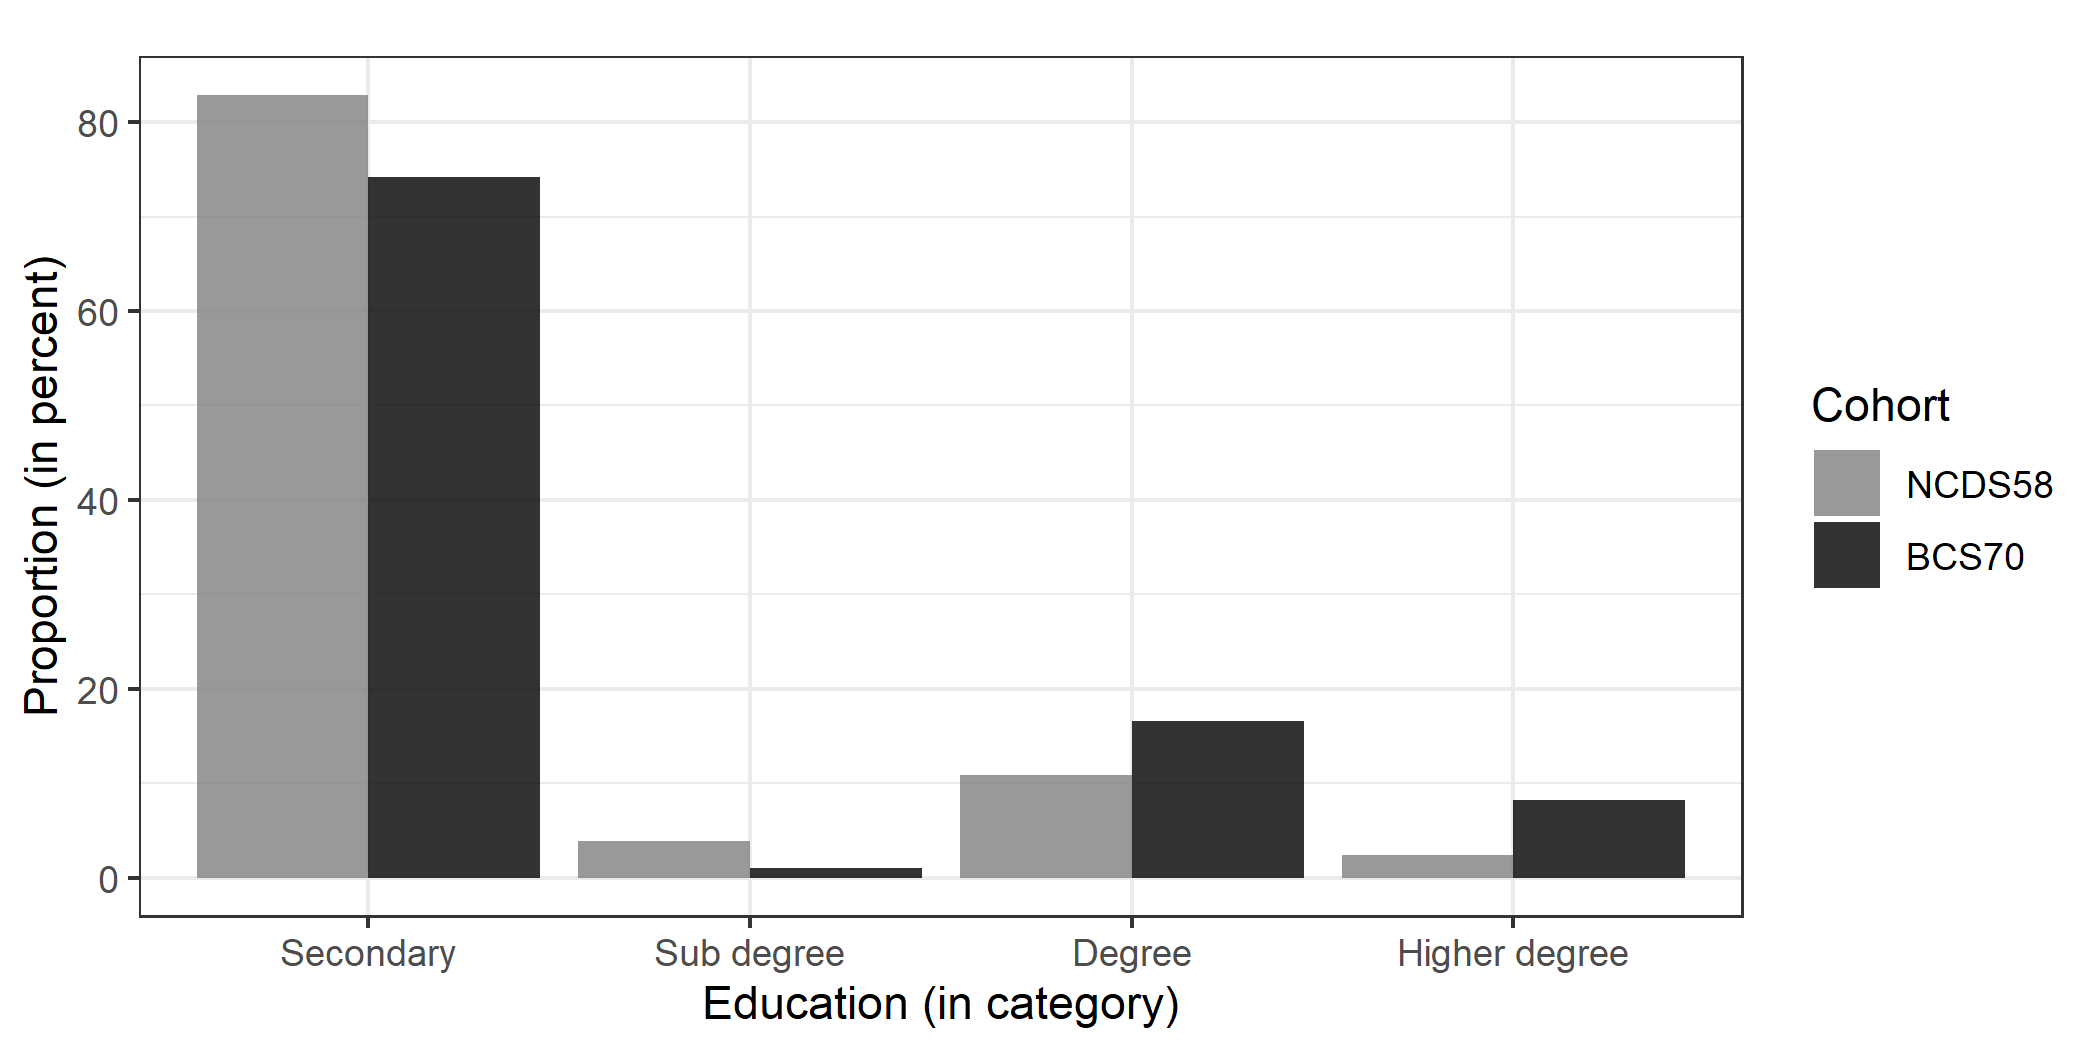
\includegraphics[width=\linewidth]{chap2/graphic/stat-educ-child-short.png}
	\vspace{-3em}
	\justify\singlespacing\footnotesize{\textit{Notes:} This figure presents the distribution of child education for the NCDS58 and BCS70 cohorts. Education corresponds to the highest academic qualification obtained by the child. Education levels are grouped into four categories for readability.}
\end{figure}

\begin{figure}[!htb]
    \centering
    \caption{Parental education distribution}
    \label{chap2-fig:stat-educ-parents}
    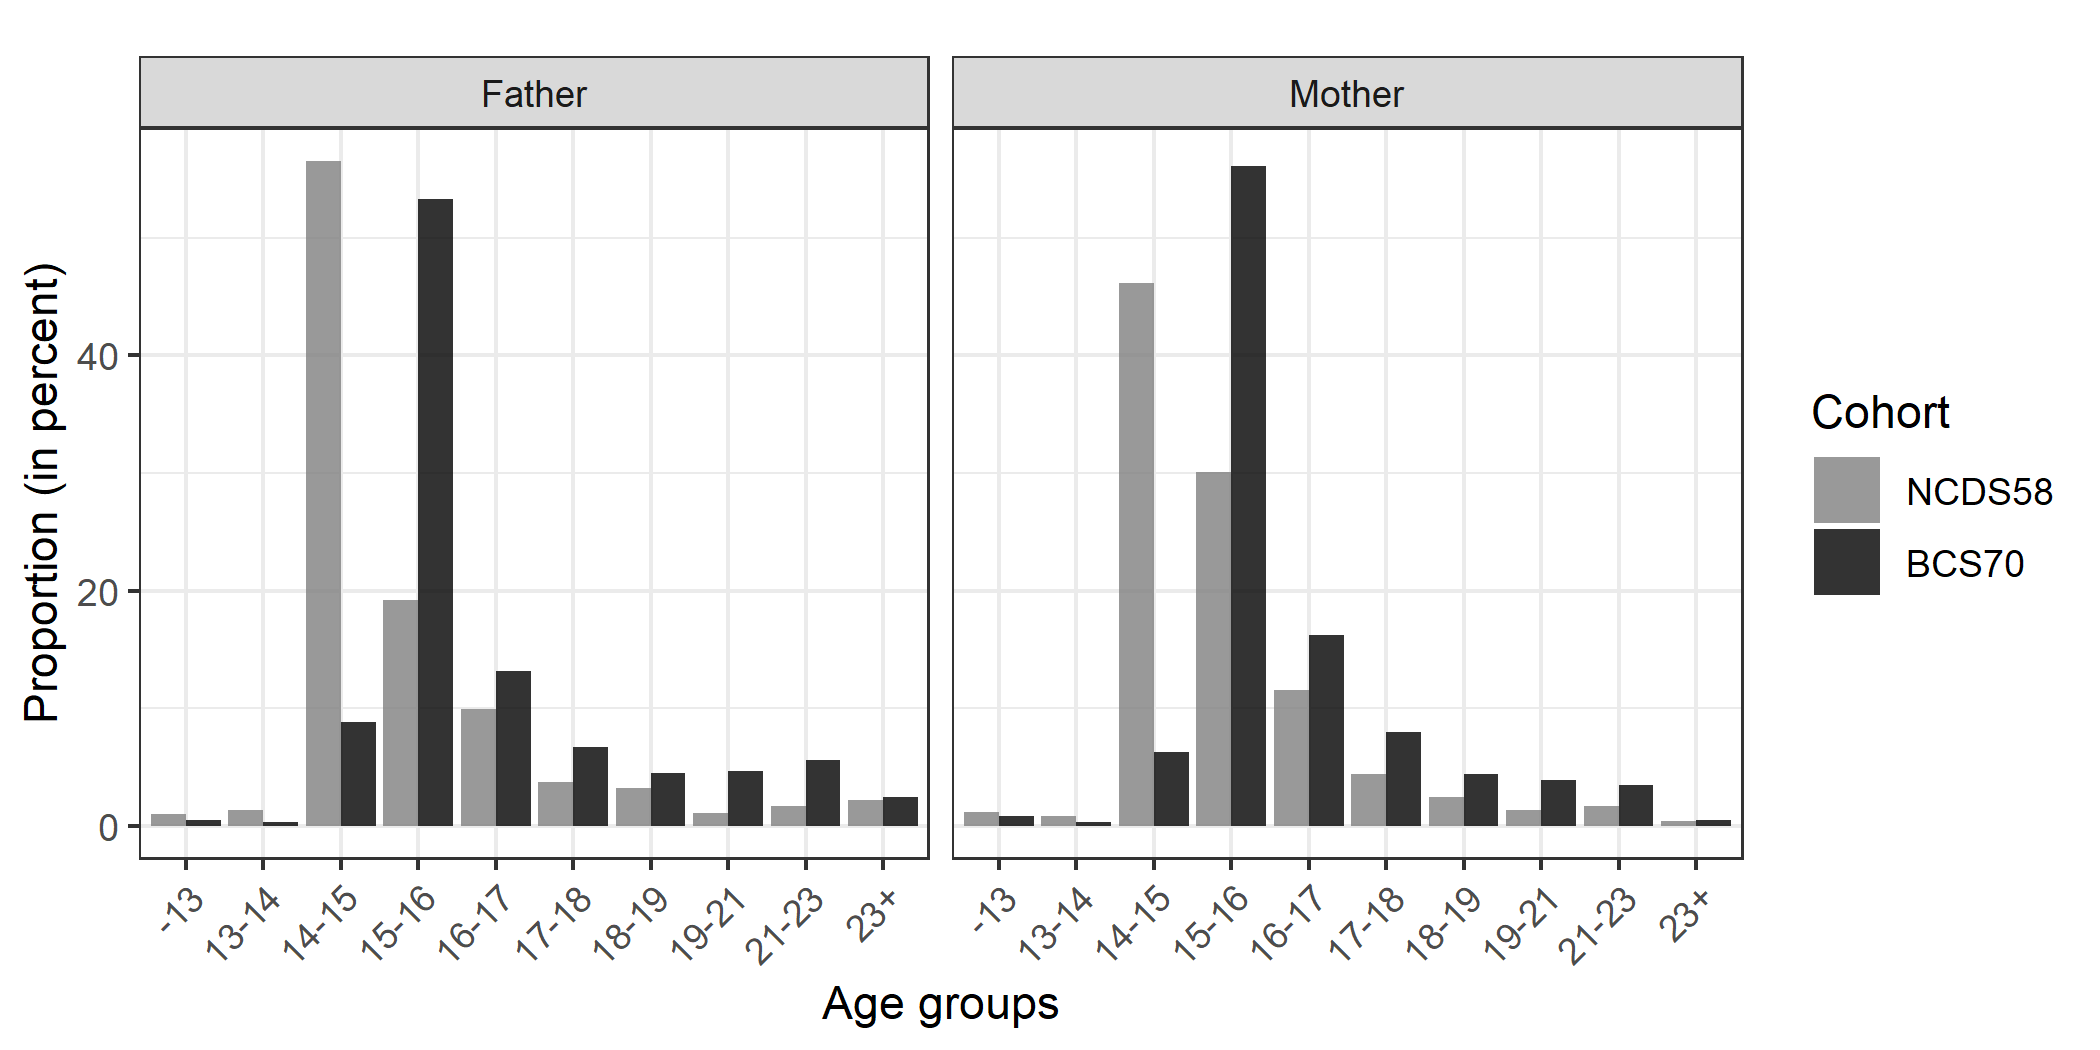
\includegraphics[width=\linewidth]{chap2/graphic/stat-educ-parents.png}
	\vspace{-3em}
	\justify\singlespacing\footnotesize{\textit{Notes:} This figure presents the distribution of parents' education for the NCDS58 and BCS70 cohorts. Parental education refers to the age at which parents left school that is used as a proxy. Education levels at the bottom and top are grouped for readability.}
\end{figure}

\textbf{Occupational structure.} In the data, occupations are reported according to e ISCO-88 categories. In Figure \ref{chap2-fig:stat-occ} we grouped occupations in three broad categories in line with the polarization literature, while Figure \ref{chap2-fig:polarize-isco88-both} performs a similar exercise using the original ISCO-88 categories. Occupations are depicted in light gray for those we place in the low-paying category, in dark grey for those in the middling category, and in black for high-paying ones. Although there are differences within the three broad categories, a clear pattern emerges both when we consider young and mature individuals. The change has been particularly large for young individual's occupations, for whom the reduction in the share of middling jobs has been marked. 

\begin{figure}[!htb]
     \centering
     \caption{Change in the probability of being in each ISCO-88 occupation in both periods}
     \label{chap2-fig:polarize-isco88-both}
     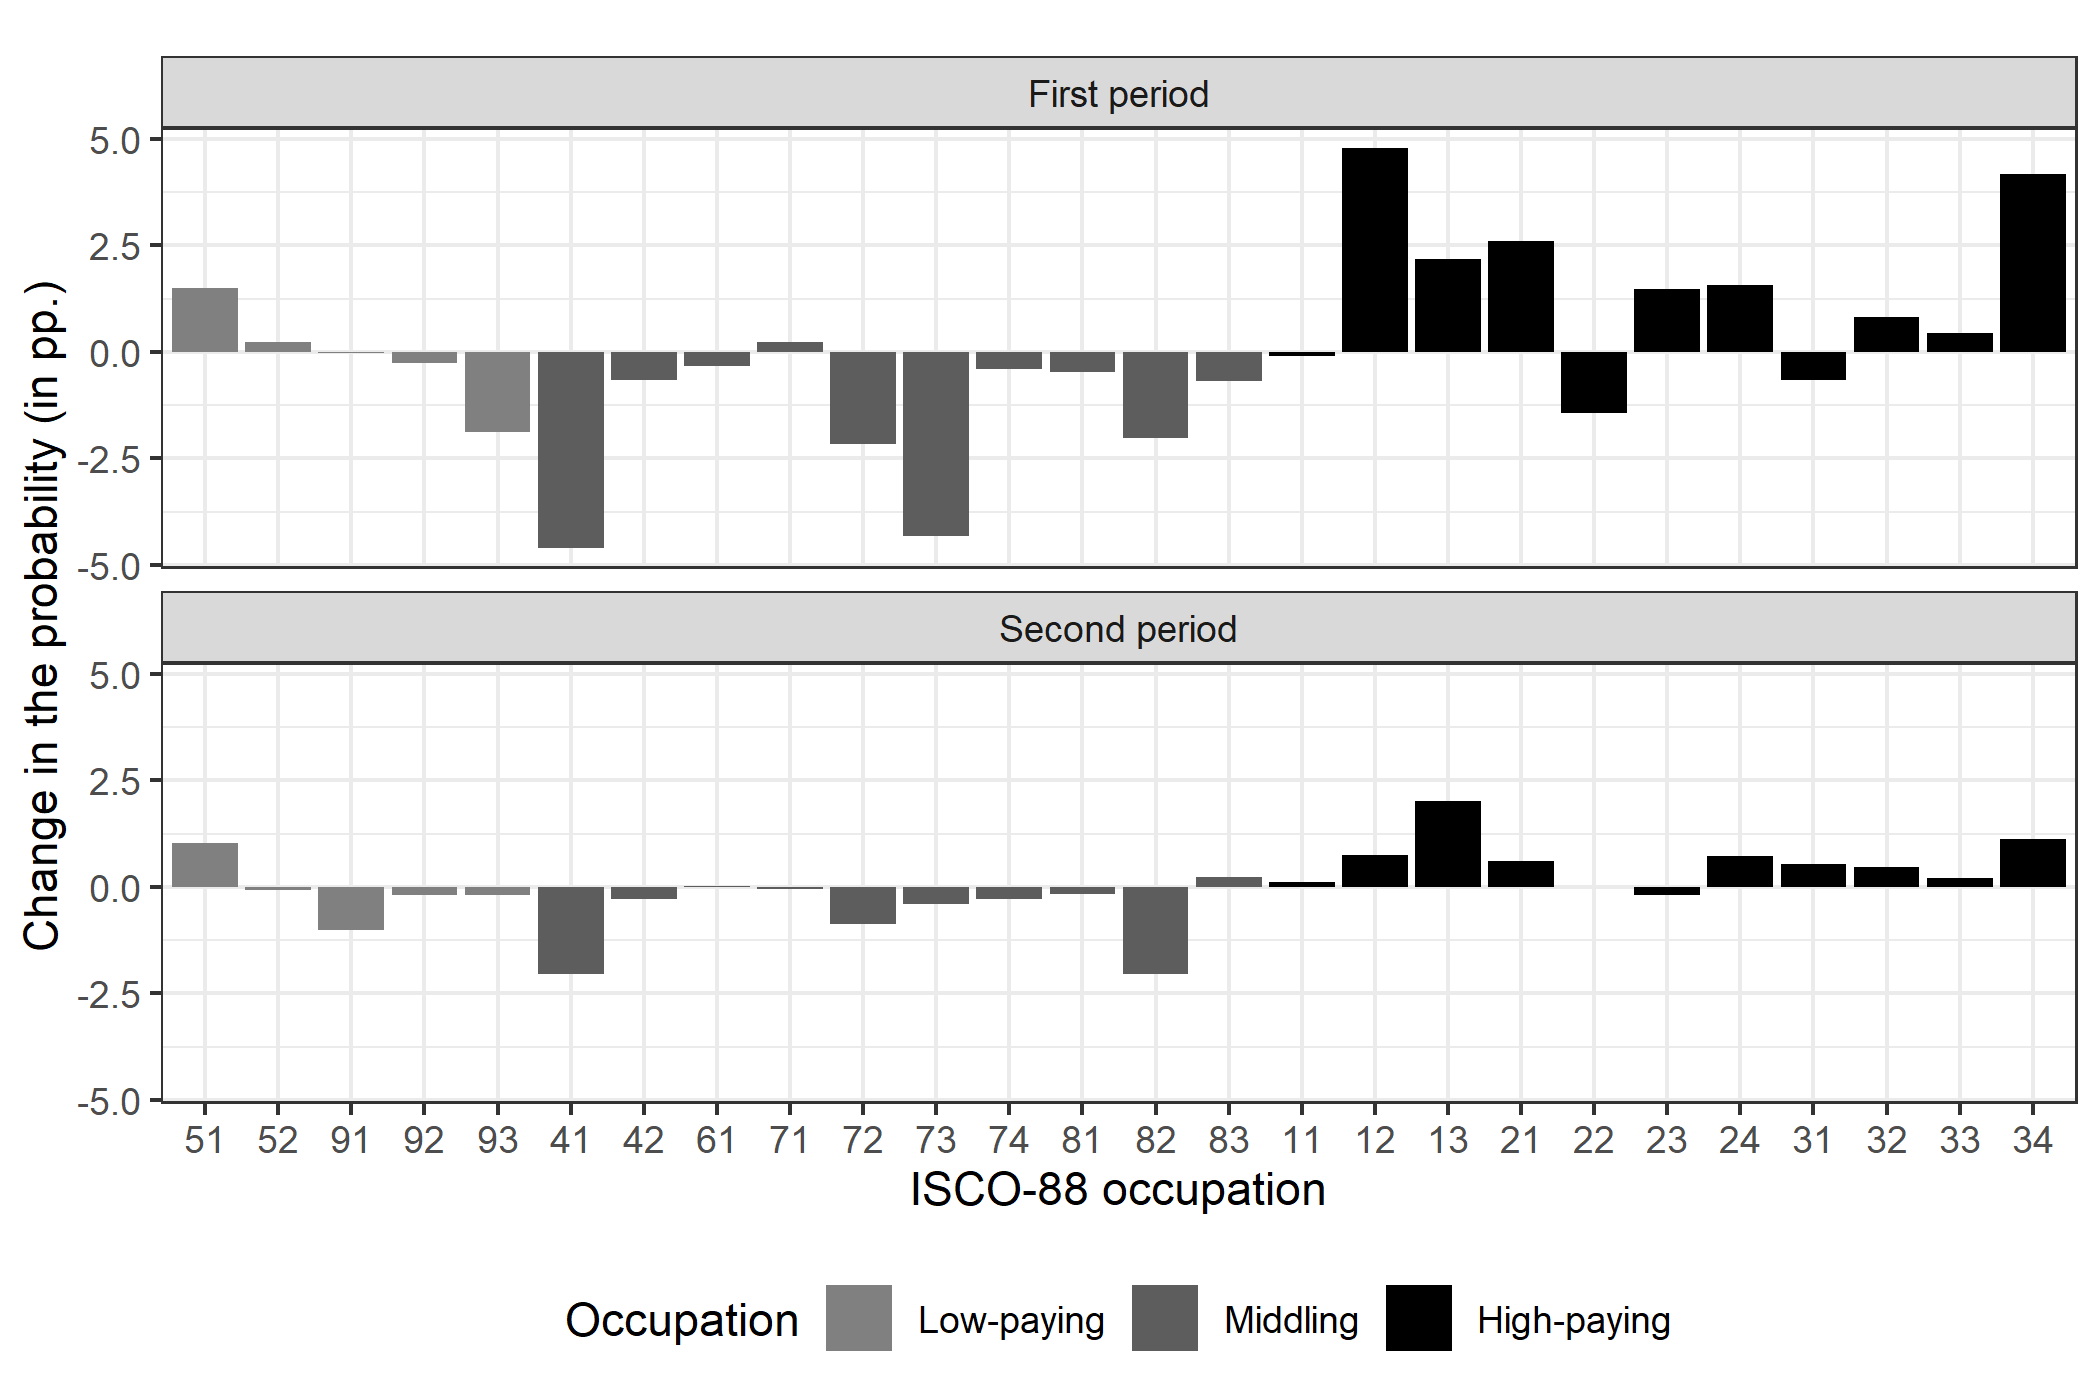
\includegraphics[width=\linewidth]{chap2/graphic/polarize-isco88-both.png}
 	\vspace{-3em}
 	\justify\singlespacing\footnotesize{\textit{Notes:} This figure presents the difference, expressed in percentage points, between the BCS70 and NCDS58 cohorts in terms of probability of being in each ISCO-88 occupation in both periods.}
\end{figure}


\subsubsection{The Labour Force Survey (1981-2012)}\label{chap2-app-data-LFS}

As a complementary dataset we use the Labor Force Survey (LFS). It is a random sampling of households living in the UK and collects data on labour market status and, since 1993, wages. The LFS was conducted every two years until 1983, then annually until 1992, and quarterly since then. It has the advantage of giving details on the occupation and industry in which individuals work, thus allowing us to take a snapshot of the structure of employment on a given year. The survey is intended to be representative of the whole population of the UK, and currently contains around 37,000 responding households in every quarter.

We use information from the LFS for the period 1981 to 2012, these being the years defined as the first-period for the older and the second-period for the younger cohorts. Initially the information is biannual, then annual from 1983 to 1992, and after that date we use data from the second quarter, as it is the one that most closely fits with the period over which annual interviews were conducted. The structure of the data allows us to define occupations in exactly the same way as for the cohort data and provides information on the region of employment.

Figure \ref{chap2-fig:lfs-national} shows the extent of job polarization at the national level using the LFS data. The share of middling jobs has declined by over 20 percentage points from 1981 to 2012. This reduction has been offset by an increase in the share of high-paying occupations by 16 percentage points over the same period, whereas the share of low-paying jobs has increased by 7 percentage points.
\begin{figure}[!htb]
    \centering
    \caption{Job polarization at the national level (The Labour Force Survey)}
    \label{chap2-fig:lfs-national}
    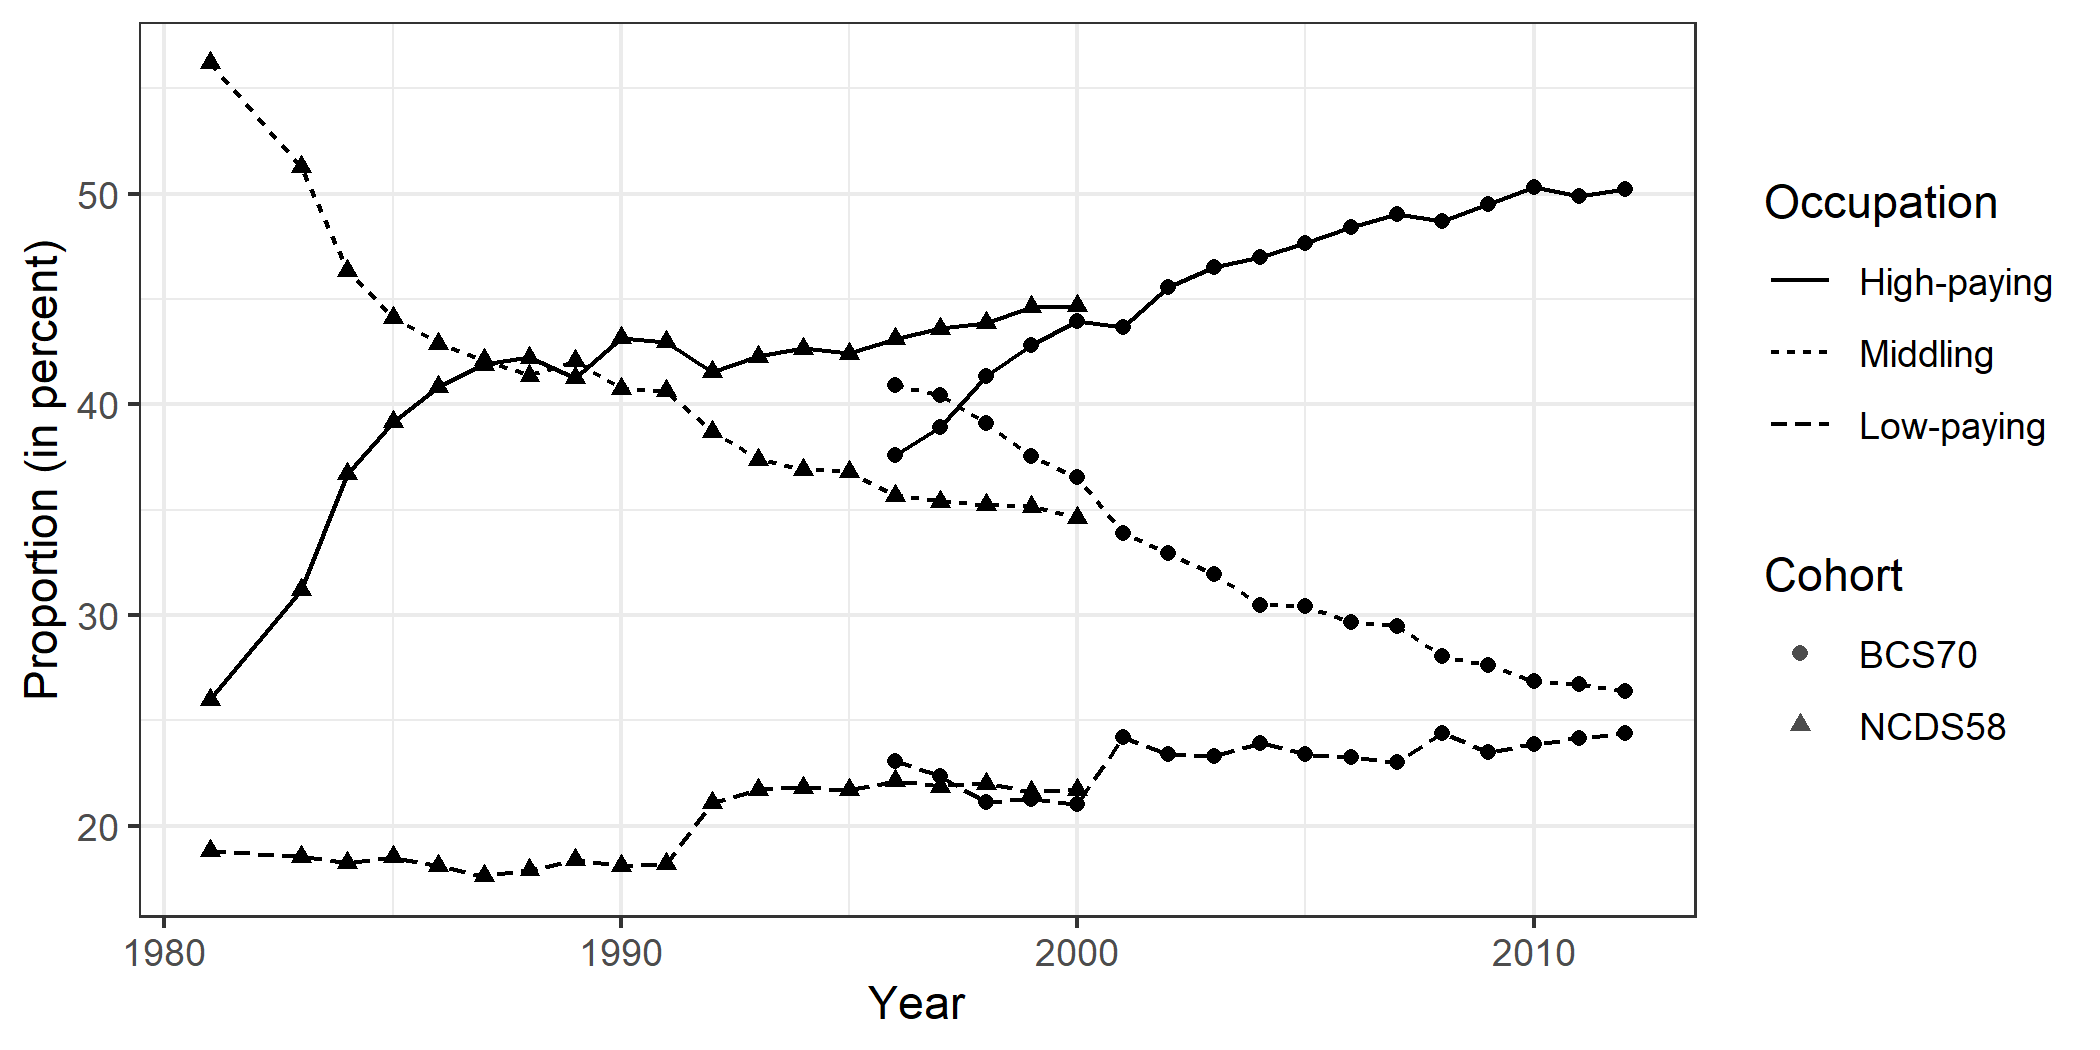
\includegraphics[width=\linewidth]{chap2/graphic/lfs-national.png}
	\vspace{-3em}
	\justify\singlespacing\footnotesize{\textit{Notes:} This figure presents the job polarization at the national level using the Labour Force Survey (LFS) data from 1981 to 2012. Curves represent the share of individuals in low-paying, middling, and high-paying occupations for the relevant age cohort in the LFS, i.e. from those born five years before to those born five years latter.}
\end{figure}

\begin{figure}[!htb]
    \centering
    \caption{Job polarization at the regional level over the lifecycle of both cohorts}
    \label{chap2-fig:lfs-regional}
    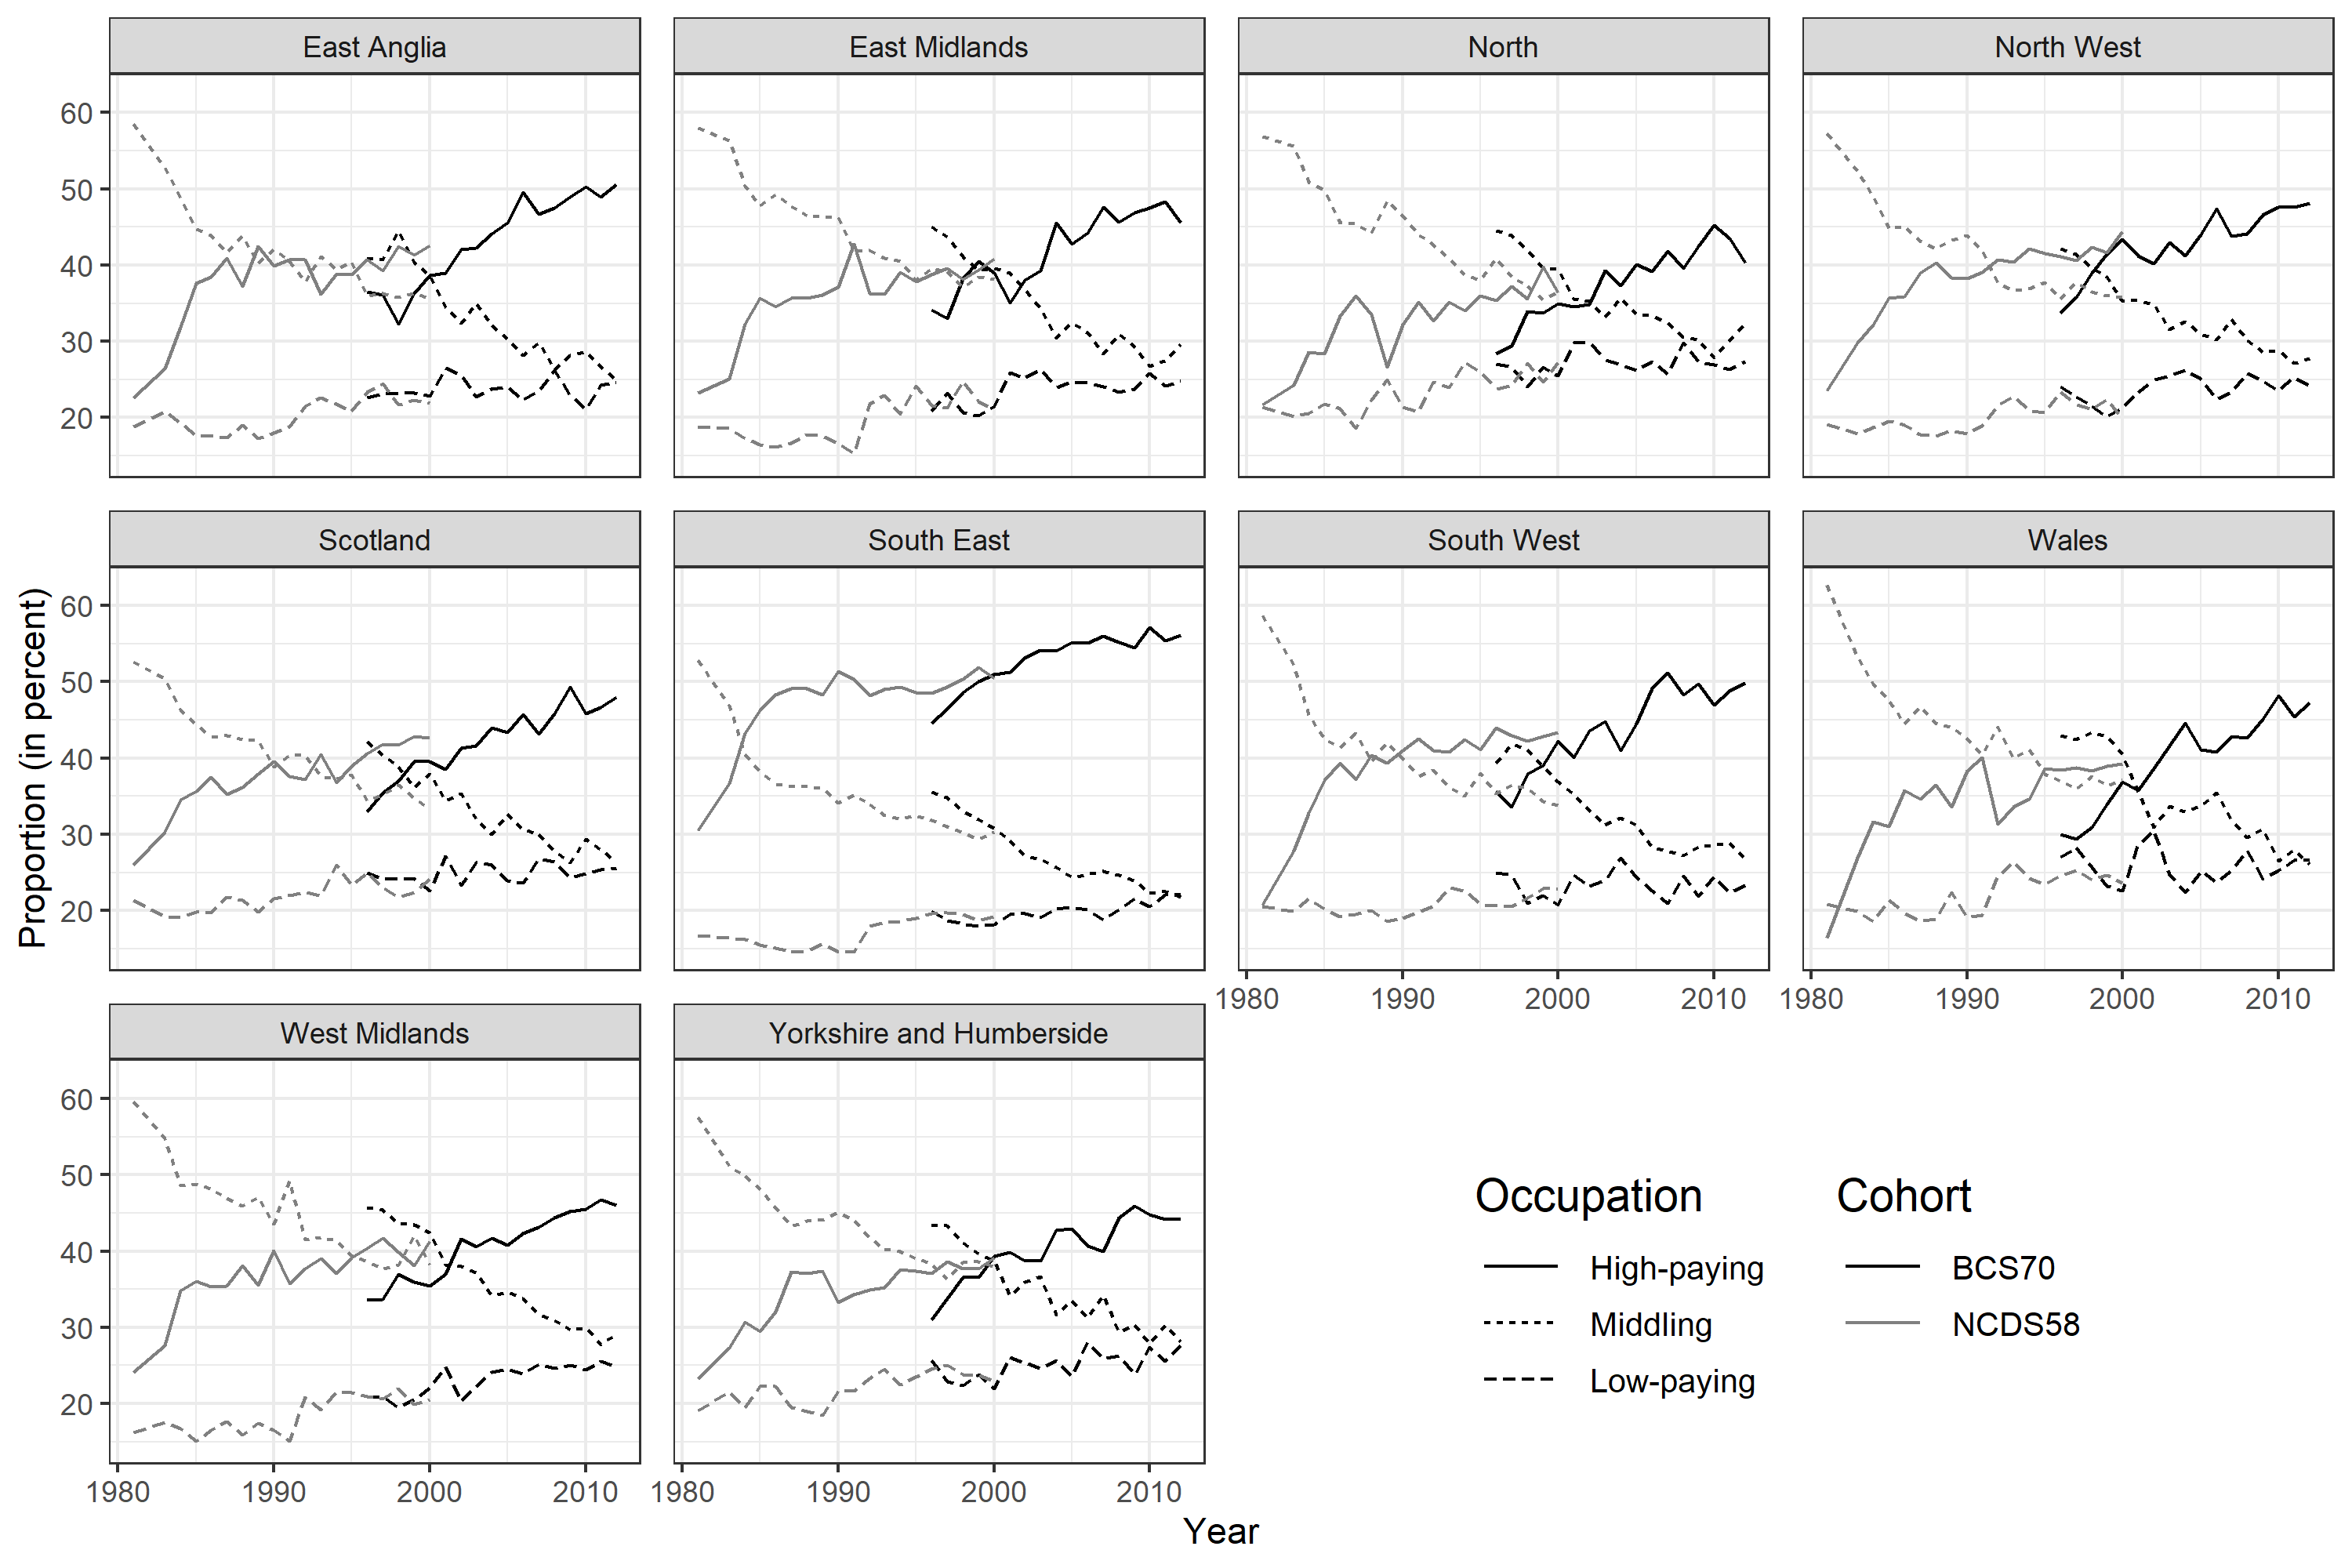
\includegraphics[width=\linewidth]{chap2/graphic/lfs-regional.png}
	\vspace{-3em}
	\justify\singlespacing\footnotesize{\textit{Notes:} This figure presents the job polarization at the regional level using the Labour Force Survey (LFS) data from 1981 to 2012. Curves represent the share of individuals in out-of-work, low-paying, middling, and high-paying occupations for the relevant age cohort in the LFS, i.e. from those born five years before to those born five years latter.}
\end{figure}

\subsubsection{Occupational classification}\label{chap2-app-data-classification}

Table \ref{chap2-tab:data-isco88} describes the classification of occupations that we use, providing an overview of ISCO-88 occupation codes along with the routine task intensities from \cite{Goos2014Explaining} and \cite{Mahutga2018Job}.
\begin{table}[!htb]
    \centering
    \begin{threeparttable}
        \caption{Overview of ISCO-88 occupation codes and routine task intensity}
        \label{chap2-tab:data-isco88}
        
\begin{tabular}{rlrr}
\toprule
\multicolumn{1}{c}{} & \multicolumn{1}{c}{} & \multicolumn{2}{c}{RTI} \\
\cmidrule(l{3pt}r{3pt}){3-4}
\textbf{Code} & \textbf{Occupation} & \textbf{GMS} & \textbf{LIS}\\
\midrule
\addlinespace[0.3em]
\multicolumn{4}{l}{\textbf{High-paying occupations}}\\
\hspace{1em}11 & Legislators and senior officials &  & -0.54\\
\hspace{1em}12 & Corporate managers & -0.75 & -0.62\\
\hspace{1em}13 & Managers of small enterprises & -1.52 & -1.41\\
\hspace{1em}21 & Physical, mathematical and engineering professionals & -0.82 & -0.70\\
\hspace{1em}22 & Life science and health professionals & -1.00 & -0.88\\
\hspace{1em}23 & Teaching professionals &  & -1.43\\
\hspace{1em}24 & Other professionals & -0.73 & -0.61\\
\hspace{1em}31 & Physical, mathematical and engineering associate professionals & -0.40 & -0.27\\
\hspace{1em}32 & Life science and health associate professionals & -0.33 & -0.20\\
\hspace{1em}33 & Teaching associate professionals &  & -1.33\\
\hspace{1em}34 & Other associate professionals & -0.44 & -0.32\\
\addlinespace[0.3em]
\multicolumn{4}{l}{\textbf{Middling occupations}}\\
\hspace{1em}41 & Office clerks & 2.24 & 2.39\\
\hspace{1em}42 & Customer service clerks & 1.41 & 1.55\\
\hspace{1em}61 & Skilled agricultural and fishery workers &  & 0.16\\
\hspace{1em}71 & Extraction and building trades workers & -0.19 & -0.06\\
\hspace{1em}72 & Metal, machinery and related trade work & 0.46 & 0.59\\
\hspace{1em}73 & Precision, handicraft, craft printing and related trade workers & 1.59 & 1.73\\
\hspace{1em}74 & Other craft and related trade workers & 1.24 & 1.38\\
\hspace{1em}81 & Stationary plant and related operators & 0.32 & 0.46\\
\hspace{1em}82 & Machine operators and assemblers & 0.49 & 0.63\\
\hspace{1em}83 & Drivers and mobile plant operators & -1.50 & -1.38\\
\addlinespace[0.3em]
\multicolumn{4}{l}{\textbf{Low-paying occupations}}\\
\hspace{1em}51 & Personal and protective service workers & -0.60 & -0.47\\
\hspace{1em}52 & Models, salespersons and demonstrators & 0.05 & 0.18\\
\hspace{1em}91 & Sales and service elementary occupations & 0.03 & 0.16\\
\hspace{1em}92 & Agricultural, fishery and related labourers &  & 0.39\\
\hspace{1em}93 & Laborers in mining, construction, manufacturing and transport & 0.45 & 0.58\\
\bottomrule
\end{tabular}

        \begin{tablenotes}[flushleft]
            \footnotesize{\item \textit{Notes}: This table provides an overview of ISCO-88 occupation codes and their corresponding Routine Task Intensity (RTI) from \cite{Goos2014Explaining} (GMS) and \cite{Mahutga2018Job} (LIS). Occupation groups (high-paying, middling and low-paying) correspond to those from \cite{Goos2014Explaining}, except for occupations 11, 23, 34, 61 and 92 that were removed from their analysis. We add these missing occupations to categories according to closest occupations, hence, relying on the 1-digit ISCO-88 classification.}
        \end{tablenotes}
    \end{threeparttable}
\end{table}
Table \ref{chap2-tab:stat-cohper} displays the shares of the various activity status and occupational categories.
\begin{table}[!htb]
    \centering
    \caption{Summary statistics - Cohort data per period}
    \label{chap2-tab:stat-cohper}
    \begin{threeparttable}
        % \setlength{\tabcolsep}{3pt}
        
\begin{tabular}{lrrrrrrrr}
\toprule
\multicolumn{1}{c}{} & \multicolumn{4}{c}{NCDS58 - N = 6780} & \multicolumn{4}{c}{BCS70 - N = 7992} \\
\cmidrule(l{3pt}r{3pt}){2-5} \cmidrule(l{3pt}r{3pt}){6-9}
\multicolumn{1}{c}{} & \multicolumn{2}{c}{First period} & \multicolumn{2}{c}{Second period} & \multicolumn{2}{c}{First period} & \multicolumn{2}{c}{Second period} \\
\cmidrule(l{3pt}r{3pt}){2-3} \cmidrule(l{3pt}r{3pt}){4-5} \cmidrule(l{3pt}r{3pt}){6-7} \cmidrule(l{3pt}r{3pt}){8-9}
Variable & Mean & SD & Mean & SD & Mean & SD & Mean & SD\\
\midrule
Activity - Employee & 0.74 & 0.44 & 0.74 & 0.44 & 0.78 & 0.42 & 0.72 & 0.45\\
Activity - Self-employed & 0.05 & 0.21 & 0.12 & 0.33 & 0.06 & 0.24 & 0.14 & 0.35\\
Activity - Unemployed & 0.05 & 0.23 & 0.02 & 0.14 & 0.02 & 0.16 & 0.02 & 0.14\\
Activity - in Education & 0.02 & 0.15 & 0.01 & 0.08 & 0.03 & 0.16 & 0.00 & 0.06\\
Activity - Inactive & 0.14 & 0.34 & 0.12 & 0.32 & 0.11 & 0.31 & 0.11 & 0.32\\
Occupation - High-paying & 0.24 & 0.42 & 0.39 & 0.49 & 0.36 & 0.48 & 0.44 & 0.50\\
Occupation - Middling & 0.41 & 0.49 & 0.28 & 0.45 & 0.33 & 0.47 & 0.24 & 0.43\\
Occupation - Low-paying & 0.14 & 0.35 & 0.19 & 0.39 & 0.15 & 0.36 & 0.18 & 0.39\\
Occupation - Out-of-work & 0.19 & 0.39 & 0.14 & 0.34 & 0.13 & 0.34 & 0.14 & 0.34\\
Occupation - in Education & 0.02 & 0.15 & 0.01 & 0.08 & 0.03 & 0.16 & 0.00 & 0.06\\
Pay & 19.06 & 7.23 & 30.35 & 24.20 & 25.21 & 16.47 & 36.01 & 25.54\\
\bottomrule
\end{tabular}

        \begin{tablenotes}[flushleft]
            \footnotesize{\item \textit{Notes}: This table provides summary statistics for individual time-variant data from the BCS70 and NCDS58 according to the period.}
        \end{tablenotes}
    \end{threeparttable}
\end{table}
Table \ref{chap2-tab:stat-pay} reports the average weekly pay by occupation in the cohort data. Weekly pay is more concentrated for young individuals than for mature ones, as wages tend to grow faster with age for those in high-paying occupations. The table indicates that the average pay has increased for every type of occupation between both cohorts. The change across cohort of pay at age 42 is roughly the same for the three categories, lying between 14 and 15\%. In contrast, for young individuals, the change has been much larger for those in high-paying occupations (50\%) than for the other two groups (13 and 20\%, respectively, in low-paying and middling occupations).

\begin{table}[!htb]
    \centering
    \caption{Average weekly pay by occupation (in 1970£)}
    \label{chap2-tab:stat-pay}
    \begin{threeparttable}
        \setlength{\tabcolsep}{18pt}
        \begin{tabular}{l D{.}{.}{3.3} D{.}{.}{3.3} D{.}{.}{3.3} D{.}{.}{3.3}}
\toprule
\multicolumn{1}{c}{} & \multicolumn{2}{c}{First period} & \multicolumn{2}{c}{Second period} \\
\cmidrule(l{3pt}r{3pt}){2-3} \cmidrule(l{3pt}r{3pt}){4-5}
Occupation & \multicolumn{1}{c}{NCDS58} & \multicolumn{1}{c}{BCS70} & \multicolumn{1}{c}{NCDS58} & \multicolumn{1}{c}{BCS70}\\
\midrule
Low-paying & 17.05 & 19.35 & 17.75 & 20.25\\
 & (0.30) & (0.61) & (0.39) & (0.37)\\
Middling & 19.60 & 23.42 & 25.26 & 29.07\\
 & (0.16) & (0.34) & (0.45) & (0.39)\\
High-paying & 19.51 & 29.23 & 40.82 & 46.64\\
 & (0.17) & (0.40) & (0.64) & (0.55)\\
\bottomrule
\end{tabular}

        \begin{tablenotes}[flushleft]
            \footnotesize{\item \textit{Notes}: This table presents the average weekly pay, expressed in 1970£, in each first- and second-period occupations for the NCDS58 and BCS70 cohorts. Standard errors between parentheses. We exclude the very bottom and top of the pay distribution for each cohort, i.e. pay which are below £1 and above £300.}
        \end{tablenotes}
    \end{threeparttable}
\end{table}

Occupations are also characterized by different educational requirements. Note, however, that a comparison across the two cohorts is not straight forward as the overall educational attainment of the population has increased, as seen in Figure \ref{chap2-fig:stat-educ-child-short}. Because of these changes, Table \ref{chap2-tab:stat-educ} reports average education by occupation using the peer-inclusive downward-looking ranking. As well as our three employment categories we also report the educational attainment of those who are not in employment, splitting this category into those in full time education and the rest of those who are out-of-work (unemployed or not participating).\footnote{In our data, child education is time invariant because we consider the highest qualification ever obtained. Although some individuals may still appear in the occupational category full-time education, their educational level is the one they will obtain in the future.} When we do not split this category we find that average education is rather high, this being the combination of the low attainment of those not participating or unemployed and the high attainment of those still in education.

\begin{table}[!htb]
    \centering
    \caption{Average education by occupations}
    \label{chap2-tab:stat-educ}
    \begin{threeparttable}
        \setlength{\tabcolsep}{18pt}
        \begin{tabular}{l D{.}{.}{3.3} D{.}{.}{3.3} D{.}{.}{3.3} D{.}{.}{3.3}}
\toprule
\multicolumn{1}{c}{} & \multicolumn{2}{c}{First period} & \multicolumn{2}{c}{Second period} \\
\cmidrule(l{3pt}r{3pt}){2-3} \cmidrule(l{3pt}r{3pt}){4-5}
Occupation & \multicolumn{1}{c}{NCDS58} & \multicolumn{1}{c}{BCS70} & \multicolumn{1}{c}{NCDS58} & \multicolumn{1}{c}{BCS70}\\
\midrule
Out-of-work & 0.55 & 0.51 & 0.54 & 0.54\\
 & (0.01) & (0.01) & (0.01) & (0.01)\\
Education & 0.89 & 0.79 & 0.84 & 0.62\\
 & (0.01) & (0.01) & (0.03) & (0.05)\\
Low-paying & 0.54 & 0.52 & 0.52 & 0.51\\
 & (0.01) & (0.01) & (0.00) & (0.00)\\
Middling & 0.58 & 0.54 & 0.55 & 0.53\\
 & (0.00) & (0.00) & (0.00) & (0.00)\\
High-paying & 0.74 & 0.72 & 0.73 & 0.70\\
 & (0.01) & (0.00) & (0.00) & (0.00)\\
\bottomrule
\end{tabular}

        \begin{tablenotes}[flushleft]
            \footnotesize{\item \textit{Notes}: This table presents the average education, expressed in peer-inclusive downward-looking ranking, in each first- and second-period occupations for the NCDS58 and BCS70 cohorts. Standard errors between parentheses.}
        \end{tablenotes}
    \end{threeparttable}
\end{table}

\subsubsection{Structure of employment}\label{chap2-app-data-structure}

Table \ref{chap2-tab:proba-group4-abs} presents the probability to be in each occupation at both periods, for both cohorts. The first-period probabilities indicate that BCS70-cohort individuals are about 7.9 pp. less likely to start in middling occupations, while they are about 12.4 pp. more likely to start their careers in a high-paying occupation. The probabilities with those in education in a separate category, hence not included in out-of-work, are reported in Table \ref{chap2-tab:proba-group5-abs}. Table \ref{chap2-tab:proba-group5-cdt-short} provides the probability of being in each second-period occupation conditional on the first-period occupation, isolating those in-education from the out-of-work. 

\begin{table}[!htb]
    \centering
    \caption{Probability of being in each occupation at both periods, for both cohorts (in percent)}
    \label{chap2-tab:proba-group4-abs}
    \begin{threeparttable}
        \setlength{\tabcolsep}{10pt}
        
\begin{tabular}{lrrrrrr}
\toprule
\multicolumn{1}{c}{} & \multicolumn{3}{c}{First period} & \multicolumn{3}{c}{Second period} \\
\cmidrule(l{3pt}r{3pt}){2-4} \cmidrule(l{3pt}r{3pt}){5-7}
Occupation & BCS70 & NCDS58 & $\Delta$ & BCS70 & NCDS58 & $\Delta$\\
\midrule
Out-of-work & 16.2 & 21.3 & -5.1 & 13.9 & 14.4 & -0.4\\
Low-paying & 15.2 & 14.0 & 1.2 & 18.4 & 19.1 & -0.7\\
Middling & 33.1 & 41.2 & -8.1 & 23.8 & 28.0 & -4.2\\
High-paying & 35.6 & 23.6 & 12.1 & 43.9 & 38.5 & 5.4\\
\bottomrule
\end{tabular}

        \begin{tablenotes}[flushleft]
            \footnotesize{\item \textit{Notes}: This table shows the probability, expressed in percent, of being in each first- and second-period occupation for the BCS70 and NCDS58 cohorts. Differences between both cohorts, expressed in percentage points, are reported in the last column of both periods.}
        \end{tablenotes}
    \end{threeparttable}
\end{table}

\begin{table}[!htb]
     \centering
     \caption{Probability to be in each occupation at both periods, isolating those in-education (in percent)}
     \label{chap2-tab:proba-group5-abs}
    \begin{threeparttable}
        % \small
        \setlength{\tabcolsep}{10pt}
        
\begin{tabular}{lrrrrrr}
\toprule
\multicolumn{1}{c}{} & \multicolumn{3}{c}{First period} & \multicolumn{3}{c}{Second period} \\
\cmidrule(l{3pt}r{3pt}){2-4} \cmidrule(l{3pt}r{3pt}){5-7}
Occupation & BCS70 & NCDS58 & $\Delta$ & BCS70 & NCDS58 & $\Delta$\\
\midrule
Out-of-work & 13.5 & 19.1 & -5.6 & 13.6 & 13.7 & -0.1\\
in-Education & 2.7 & 2.2 & 0.5 & 0.3 & 0.6 & -0.3\\
Low-paying & 15.2 & 14.0 & 1.2 & 18.4 & 19.1 & -0.7\\
Middling & 33.1 & 41.2 & -8.1 & 23.8 & 28.0 & -4.2\\
High-paying & 35.6 & 23.6 & 12.1 & 43.9 & 38.5 & 5.4\\
\bottomrule
\end{tabular}

        \begin{tablenotes}[flushleft]
            \footnotesize{\item \textit{Notes}: This table shows the probability, expressed in percent, of being in each first- and second-period occupation for the BCS70 and NCDS58 cohorts. Differences between both cohorts, expressed in percentage points, are reported in the last column of both periods.}
        \end{tablenotes}
    \end{threeparttable}
\end{table}

\begin{table}[!htb]
    \centering
    \caption{Conditional probabilities of changing occupations during the career, isolating those in-education (in percent)}
    \label{chap2-tab:proba-group5-cdt-short}
    \resizebox{\textwidth}{!}{
    \begin{threeparttable}
        
\begin{tabular}{lrrrrrrrrrr}
\toprule
\multicolumn{1}{c}{} & \multicolumn{5}{c}{BCS70} & \multicolumn{5}{c}{NCDS58} \\
\cmidrule(l{3pt}r{3pt}){2-6} \cmidrule(l{3pt}r{3pt}){7-11}
Occupation & Out & Educ & Low & Mid & High & Out & Educ & Low & Mid & High\\
\midrule
Out-of-work & 37.0 & 0.7 & 28.3 & 15.2 & 18.9 & 28.5 & 0.9 & 26.9 & 22.1 & 21.6\\
in-Education & 14.0 & 0.5 & 10.7 & 11.2 & 63.7 & 10.7 & 0.0 & 5.3 & 8.0 & 76.0\\
Low-paying & 13.3 & 0.3 & 45.1 & 17.5 & 23.8 & 15.8 & 0.5 & 40.0 & 20.3 & 23.4\\
Middling & 10.2 & 0.3 & 13.8 & 44.9 & 30.8 & 9.9 & 0.5 & 15.4 & 43.4 & 30.8\\
High-paying & 8.0 & 0.2 & 8.2 & 11.0 & 72.6 & 7.6 & 0.8 & 8.1 & 12.3 & 71.2\\
\bottomrule
\end{tabular}

        \begin{tablenotes}[flushleft]
            \footnotesize{\item \textit{Notes}: Conditional probabilities with people in education included in out-of-work are reported in the paper, see table \ref{chap2-tab:proba-group4-cdt}.}
        \end{tablenotes}
    \end{threeparttable}
    }
\end{table}

Figure \ref{chap2-fig:polarize-isco88-pay-p3} presents the change in the frequencies of second period occupation according to the average weekly pay for the BCS70 cohort. 
Figure \ref{chap2-fig:polarize-rtiLIS-p3} displays the negative relationship between the probability of being in each second-period occupation according to its routine task intensity.

\begin{figure}[!htb]
    \centering
    \caption{Change in the probability of being in an occupation in the second period and average weekly pay}
    \label{chap2-fig:polarize-isco88-pay-p3}
    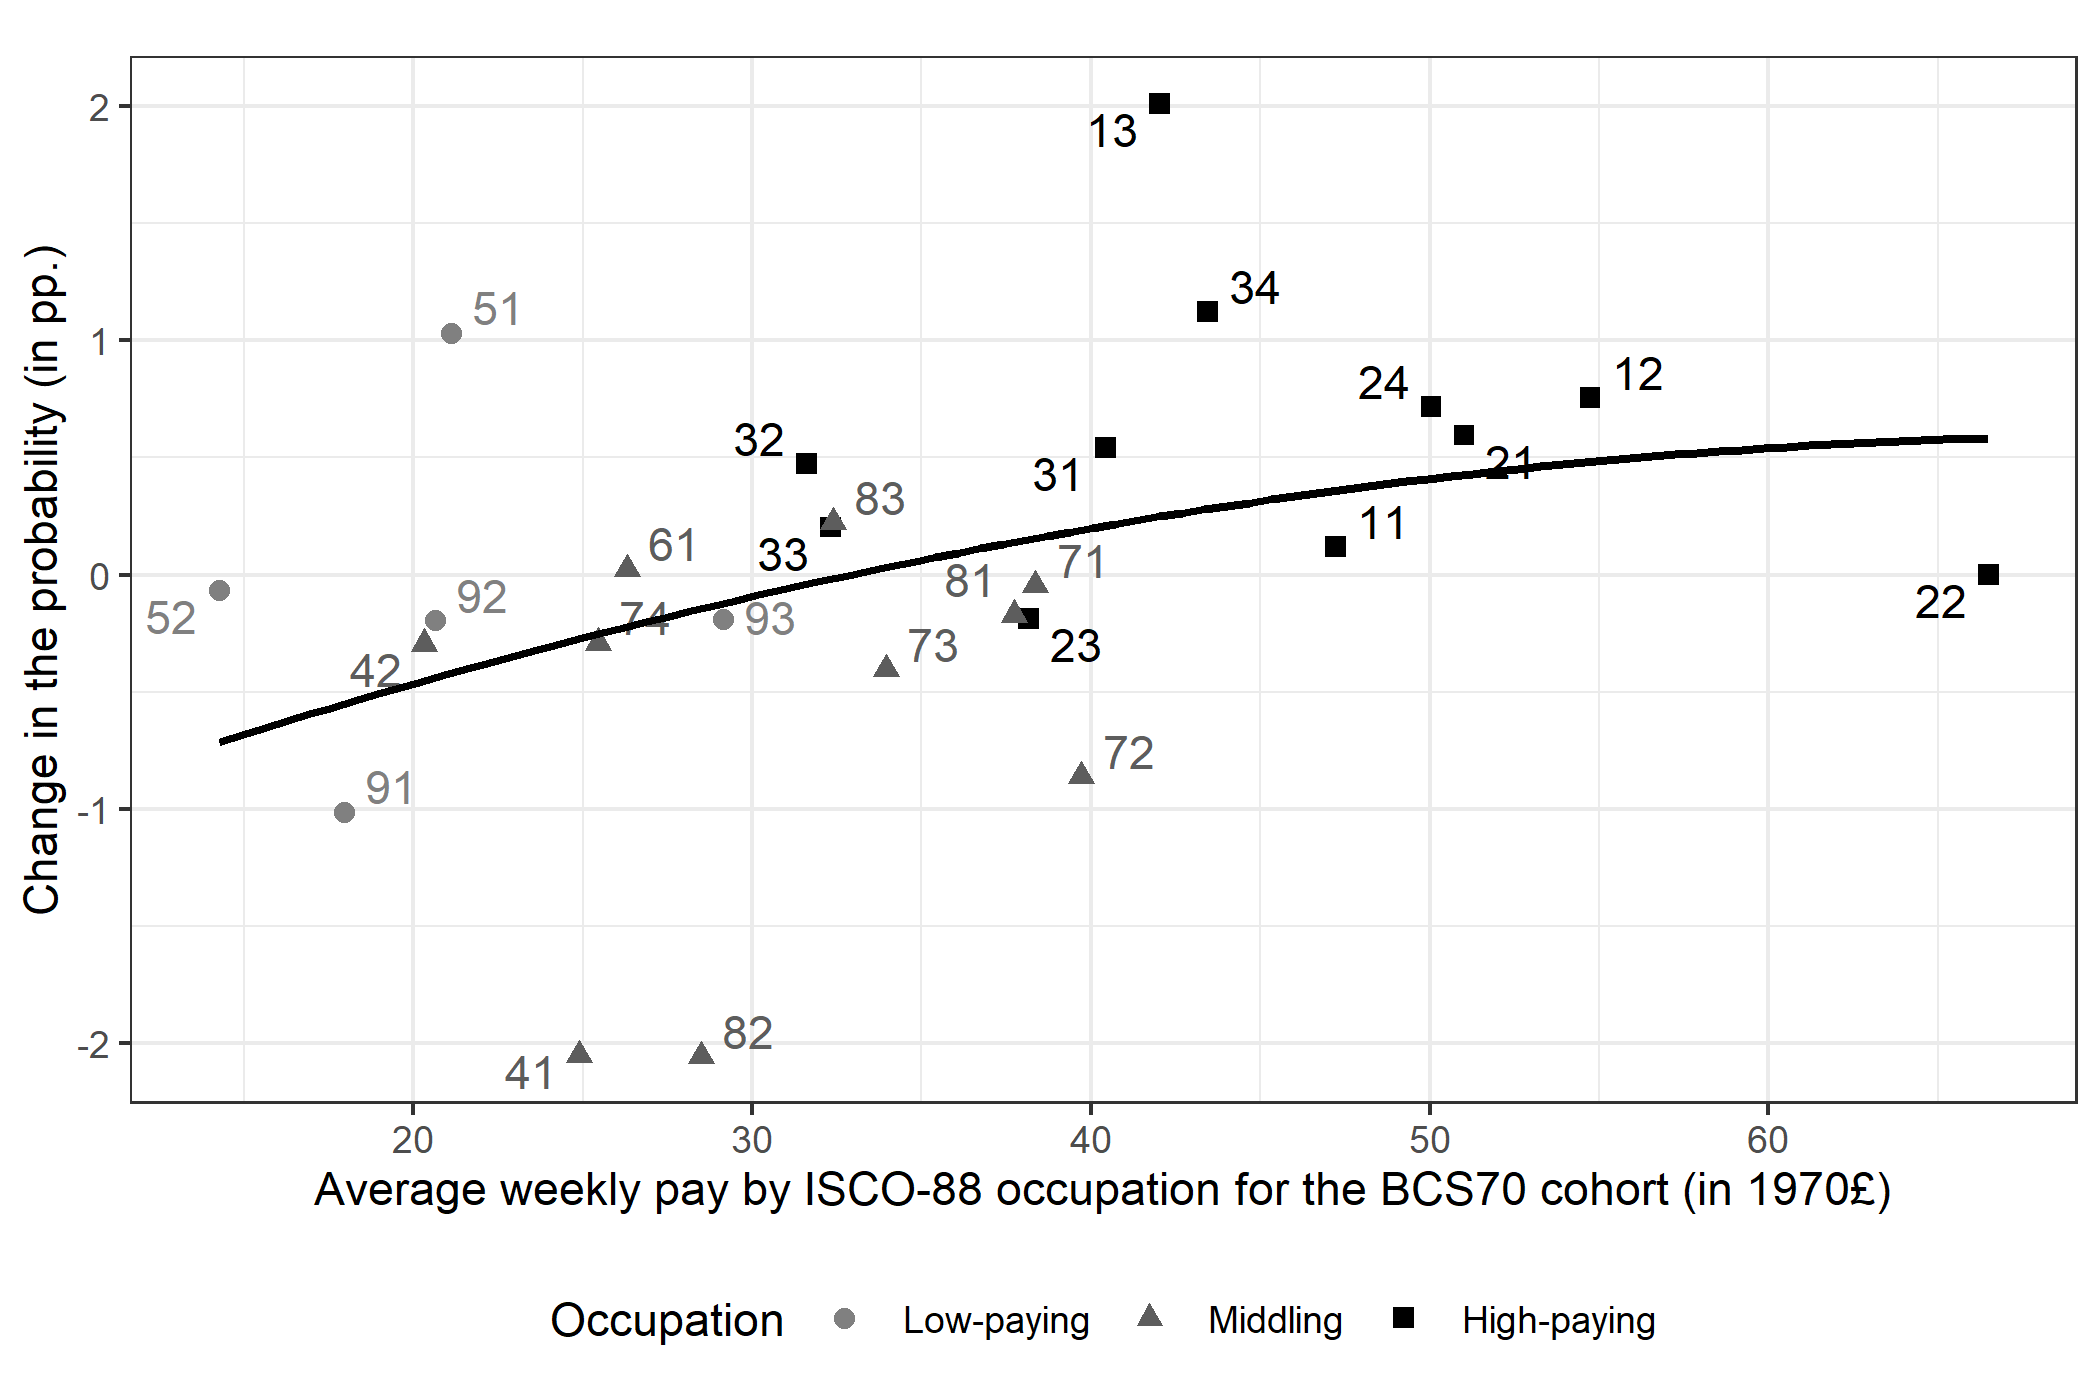
\includegraphics[width=\linewidth]{chap2/graphic/polarize-BCSpay-p3.png}
	\vspace{-3em}
	\justify\singlespacing\footnotesize{\textit{Notes:} This figure presents the positive relationship between the difference, expressed in percentage points, between the BCS70 and NCDS58 cohorts in terms of probability of being in each ISCO-88 occupation in second period and the average weekly pay, expressed in 1970£, in this occupation for the BCS70 cohort.}
\end{figure}

\begin{figure}[!htb]
    \centering
    \caption{Change in the probability of being in an occupation in the second period and routine task intensity}
    \label{chap2-fig:polarize-rtiLIS-p3}
    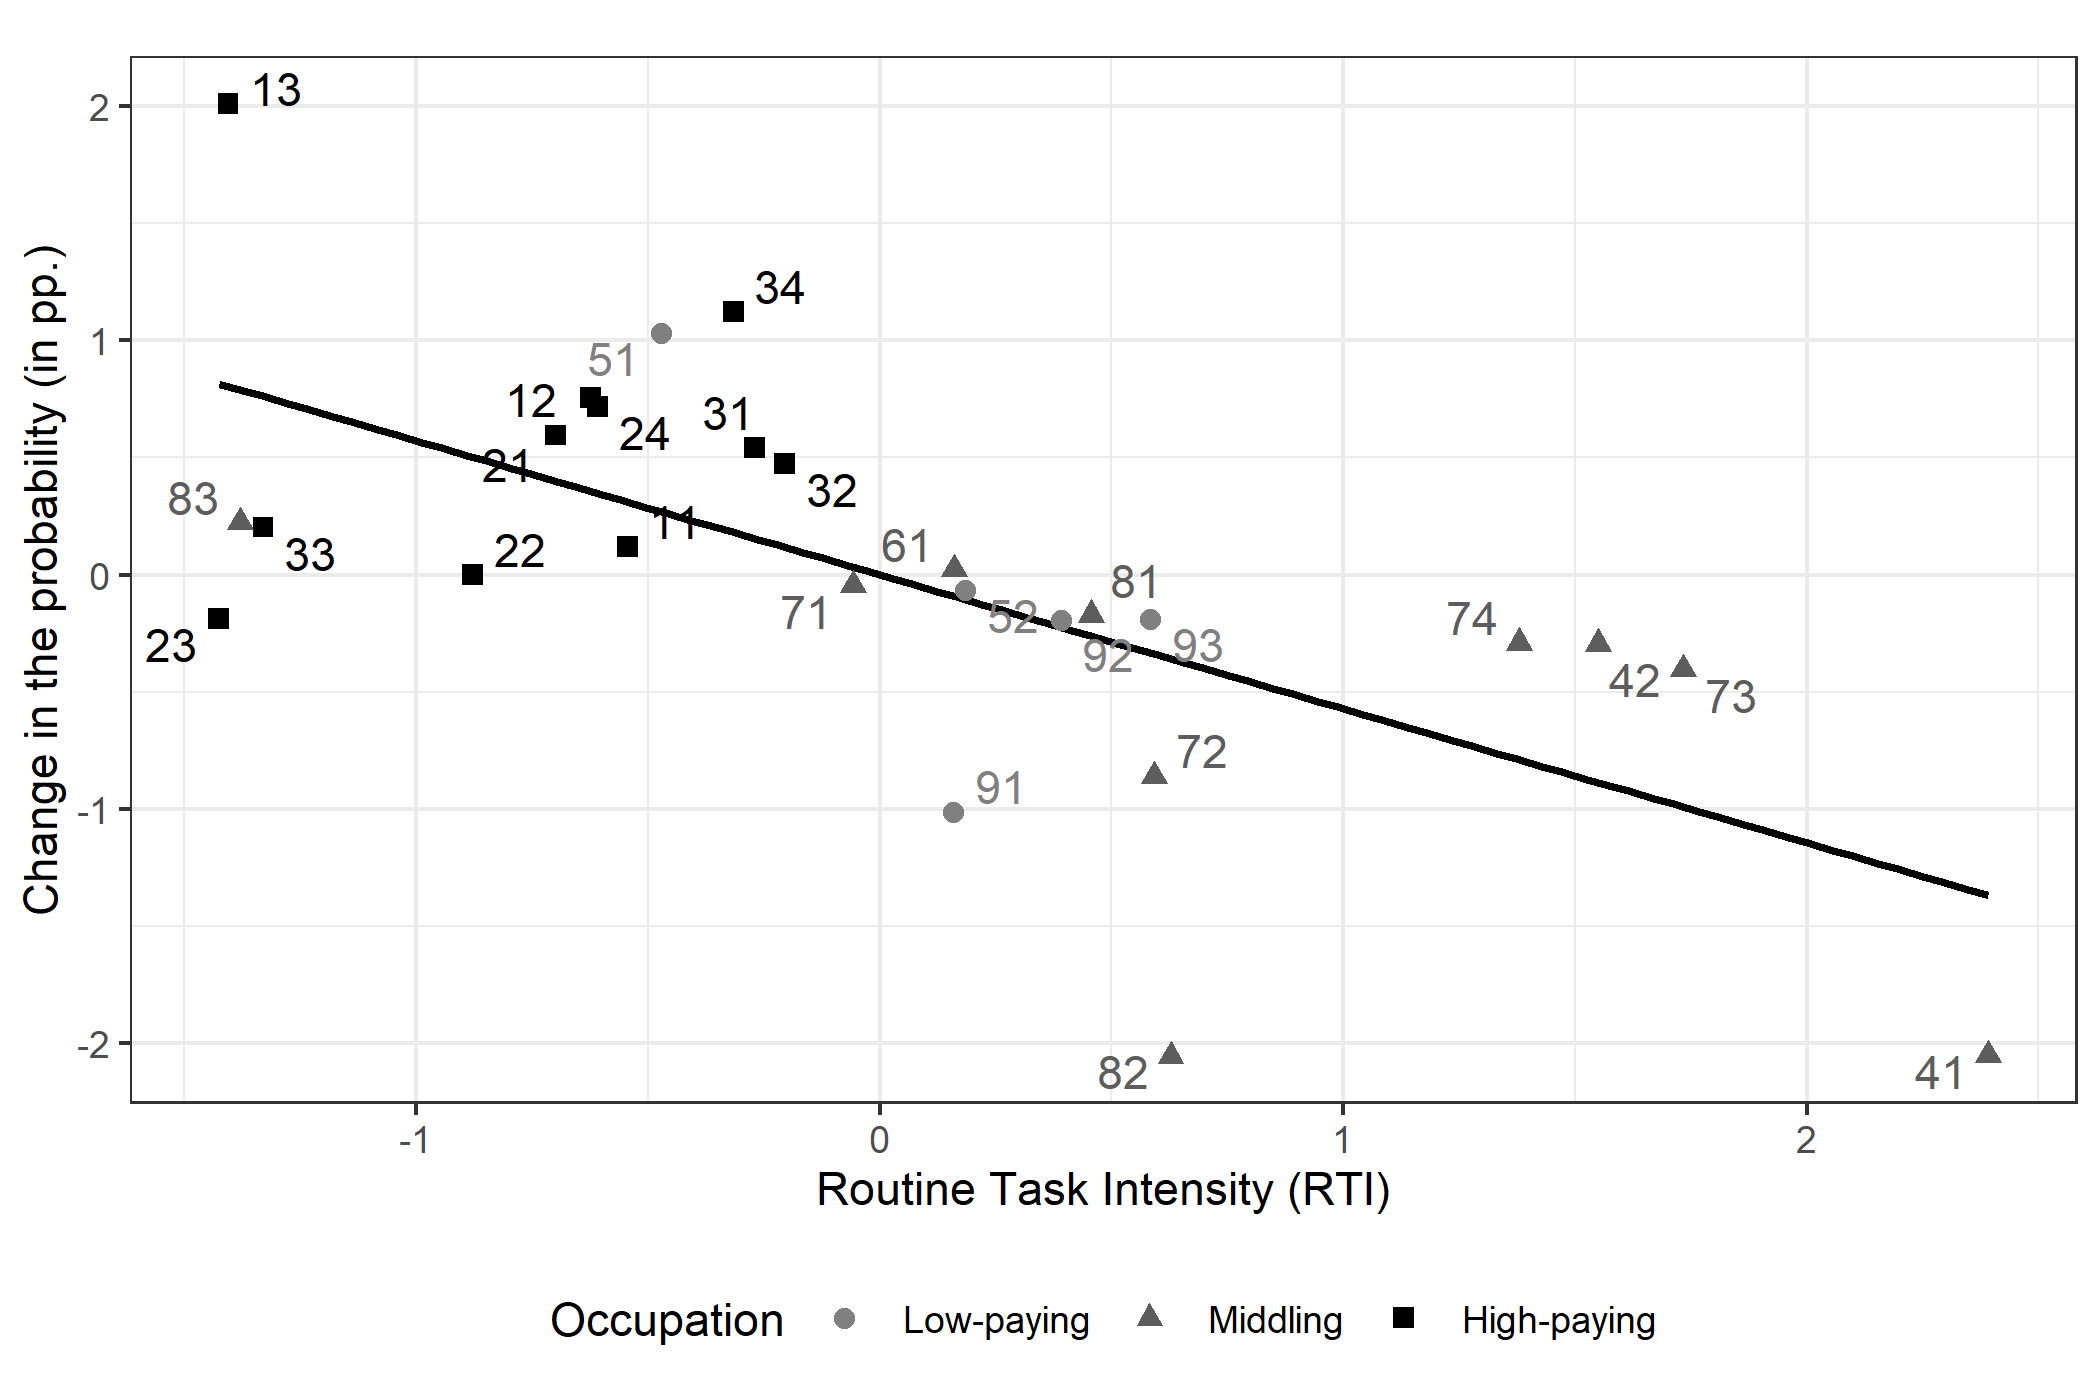
\includegraphics[width=\linewidth]{chap2/graphic/polarize-rtiLIS-p3.png}
	\vspace{-3em}
	\justify\singlespacing\footnotesize{\textit{Notes:} This figure shows the negative relationship between the difference, expressed in percentage points, between the BCS70 and NCDS58 cohorts in terms of probability of being in each ISCO-88 occupation in second period and the Routine Task Intensity (RTI) index from \cite{Mahutga2018Job}.}
\end{figure}

Lastly, Figure \ref{chap2-fig:lfs-change} reports the change in polarization in each of the regions obtained from the LFS.  

\begin{figure}[!htb]
    \centering
    \caption{Between-cohort change in the average share of total employment over the lifecycle of both cohorts (at the regional level)}
    \label{chap2-fig:lfs-change}
    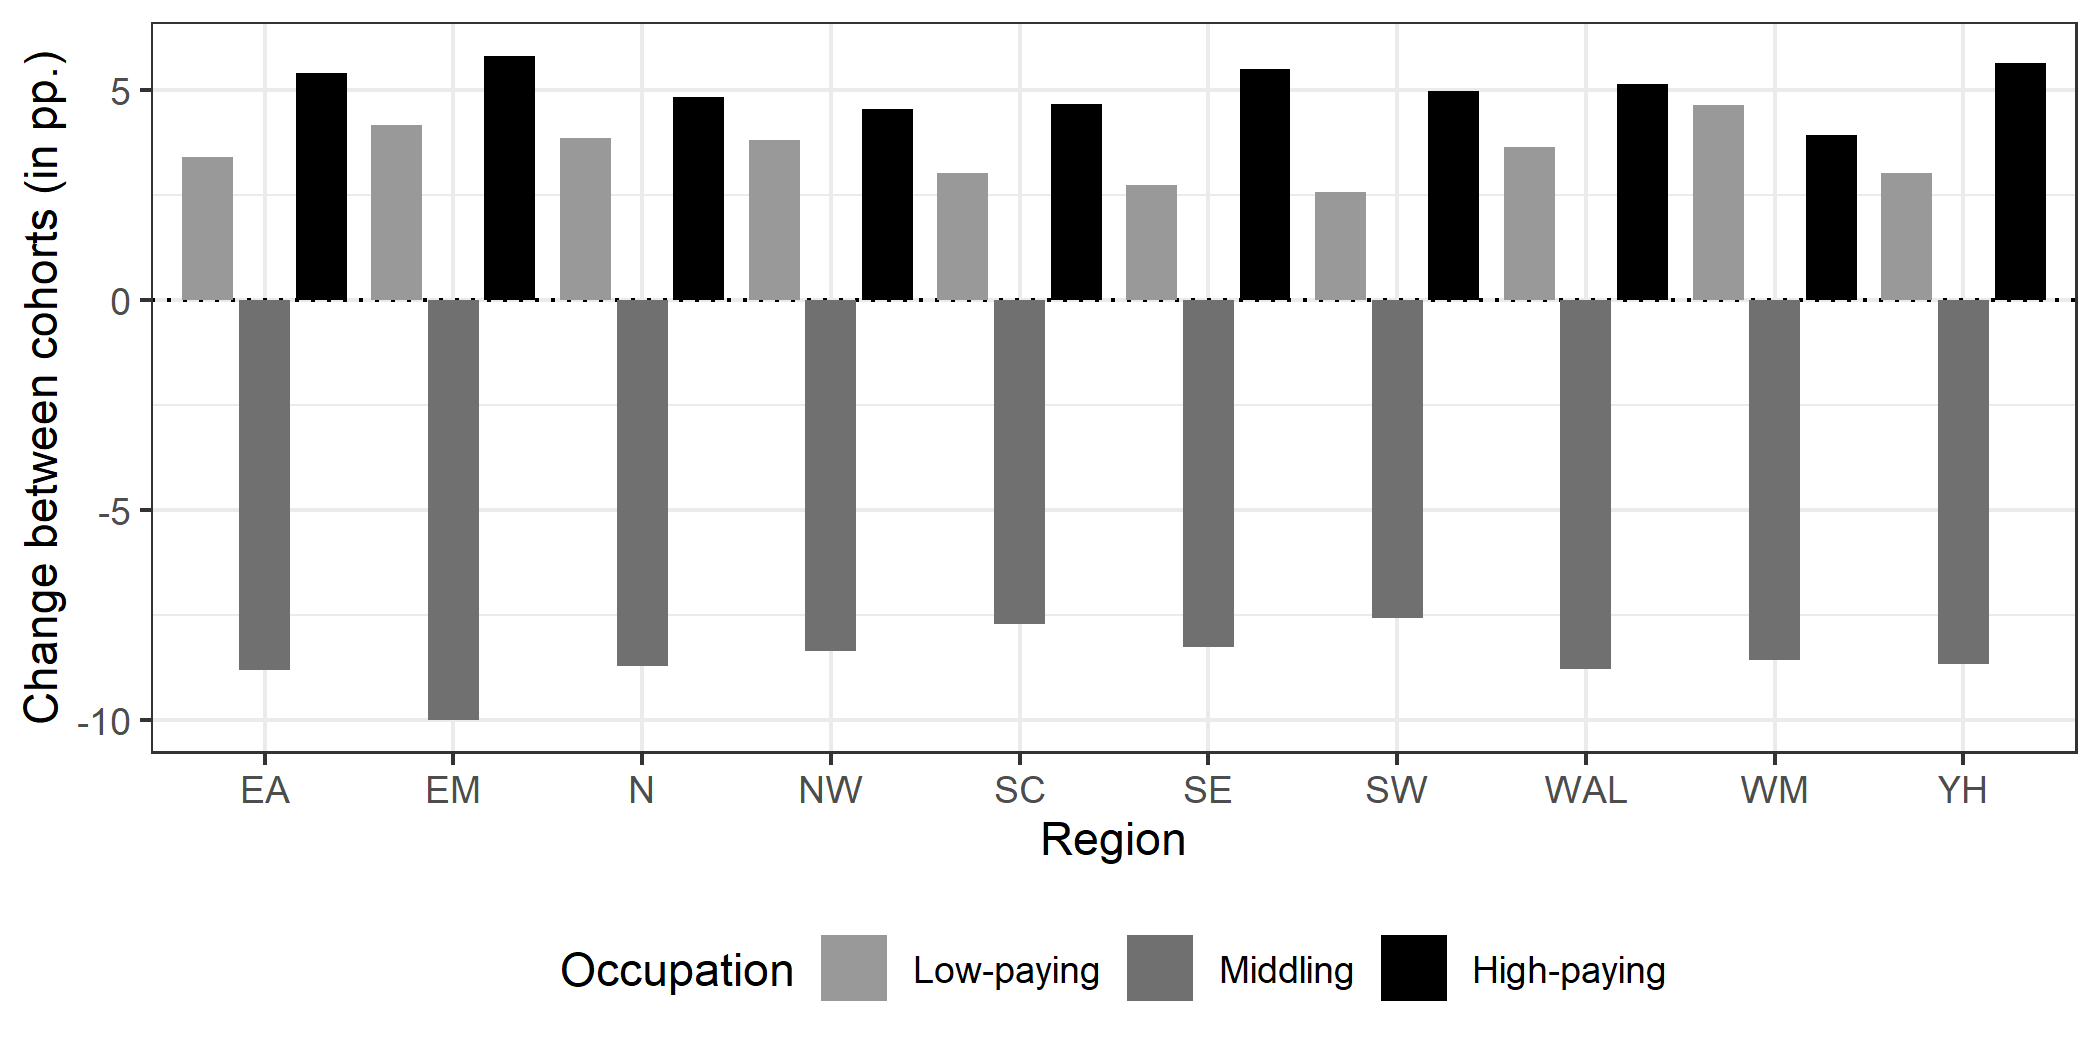
\includegraphics[width=\linewidth]{chap2/graphic/lfs-change.png}
	\vspace{-3em}
	\justify\singlespacing\footnotesize{\textit{Notes:} This figure presents the job polarization at the regional level using the Labour Force Survey data from 1981 to 2012.}
\end{figure}
    \clearpage
    \subsection{Logistic regressions}\label{chap2-app-logit}
    This appendix provides the regression tables for occupations under the multinomial and the binomial specifications of the logistic regressions. We also discuss the complementarity of both specifications to interpret coefficients as the the multinomial coefficients are relative to the baseline occupation category, namely, out-of-work.

\subsubsection{First-period occupation}

Table \ref{chap2-tab:occ-multi1-base} reports the coefficients of the \emph{multinomial} logistic regression from equation \eqref{chap2-eq:emp-multi1} for the first-period occupation. Table \ref{chap2-tab:occ-bi1-base} reports the coefficients regressions for the equivalent \emph{binomial} specification.

Each of these two estimation methods has advantages and disadvantages. Consider first the binomial logit in Table \ref{chap2-tab:occ-bi1-base}. Each regression compares the probability of being in occupation $j$ relative to the other three outcomes. In some cases, the regression is easy to interpret. For example, the regression for out-of-work compares this outcome relative to a composite of all three other occupations, i.e. being in employment. The coefficients on the Out-of-work column then tell us that for the NCDS58 cohort parental income had no effect on being out-of-work, while for the BCS70 it had a negative and significant effect. For low-paying occupations we find that parental income reduces the likelihood to be in the occupation, with the effect being three times as high for the BCS70 than for the NCDS58. The 4th column indicates that parental income increases the probability of being in a high-paying occupation (as compared to the other three outcomes) for both cohorts, although the coefficient is twice as high for the younger cohort. The interpretation of the regressions becomes harder for middling occupations as the alternative not-being-in-middling-occupations includes outcomes that are better and outcomes that are worse than middling. We find a moderate effect of parental income (-0.07) and no significant change across cohorts. Yet this may be the result of differential effects for moving up or down the occupational scale.

A solution to the above problem is to consider a multinomial logit, which compares the likelihood to be in each of the three employment categories to that of the reference group, out-of-work. The multinomial regressions have the advantage of considering simultaneously all the possible outcomes, yet they are harder to interpret as the coefficients represent odds relative to the omitted group. That is, when considering coefficients one needs to keep in mind the dynamics for the out-of-work outcome as captured by the Out-of-work column in Table \ref{chap2-tab:occ-bi1-base}. 

The results for the multinomial estimation reported in Table \ref{chap2-tab:occ-multi1-base} indicate that the likelihood to be in a high-paying occupation is strongly affected by parental income, with the coefficient doubling across cohorts (from 0.21 to 0.42). The insignificant coefficients on ``$\text{Par. Inc.}$'' indicate that, for the NCDS58 cohort, parental income does not give an advantage to get low-paying or middling jobs relative to being out of work. However, it does confer such an advantage for the younger cohort. The negative slopes reported in Figure \ref{chap2-fig:occ-multi1-pinc} are the combination of a large decline in the coefficient on parental income for those out-of-work (see the coefficient on ``$\text{Par. inc.}~\times~\text{BCS}$'' in the first column in Table \ref{chap2-tab:occ-bi1-base}) and the positive but smaller coefficients on the first two columns of Table \ref{chap2-tab:occ-multi1-base}.

\begin{table}[!htb]
    \centering
    \caption{Probability of being in each occupation at first period (multinomial)}
    \label{chap2-tab:occ-multi1-base}
    \begin{threeparttable}
        \centering
        \setlength{\tabcolsep}{15pt}
        \begin{tabular}{l D{.}{.}{5.5} D{.}{.}{5.5} D{.}{.}{5.5}}
\toprule
 & \multicolumn{3}{c}{Multinomial logit - Dep. var.: First-period occupation} \\
\cmidrule(lr){2-4}
 & \multicolumn{1}{c}{Low-paying} & \multicolumn{1}{c}{Middling} & \multicolumn{1}{c}{High-paying} \\
\midrule
Intercept              & 0.08        & 1.39^{***}  & 0.69^{***}  \\
                       & (0.07)      & (0.06)      & (0.06)      \\
BCS cohort             & 0.24^{**}   & 0.12        & 0.75^{***}  \\
                       & (0.10)      & (0.08)      & (0.09)      \\
Female                 & -0.79^{***} & -1.27^{***} & -0.99^{***} \\
                       & (0.09)      & (0.07)      & (0.08)      \\
Female $\times$ BCS    & 0.25^{**}   & -0.02       & -0.08       \\
                       & (0.12)      & (0.10)      & (0.11)      \\
Par. inc.              & -0.03       & -0.00       & 0.21^{***}  \\
                       & (0.04)      & (0.03)      & (0.04)      \\
Par. inc. $\times$ BCS & 0.10^{*}    & 0.22^{***}  & 0.41^{***}  \\
                       & (0.06)      & (0.05)      & (0.05)      \\
\midrule
Num. obs. & \multicolumn{1}{c}{14763} & \multicolumn{1}{c}{14763} & \multicolumn{1}{c}{14763}\\
\bottomrule
\end{tabular}

        \begin{tablenotes}[flushleft]
            \footnotesize{\item \textit{Notes}: 
            % Stars and SE
            $^{***}p<0.01$; $^{**}p<0.05$; $^{*}p<0.1$. Standard errors between parentheses. 
            % Baseline outcome
            Out-of-work occupation in first period is the base outcome of the multinomial logistic regression.
            % Referent group
            Male in the NCDS58 cohort is the referent group. 
            % Variables details
            Parental income in logarithm and then standardized at the cohort level.}
        \end{tablenotes}
    \end{threeparttable}
\end{table}

\begin{table}[!htb]
    \centering
    \caption{Probability of being in each occupation at first period (binomial)}
    \label{chap2-tab:occ-bi1-base}
    \begin{threeparttable}
        \centering
        % \setlength{\tabcolsep}{0pt}
        \begin{tabular}{l D{.}{.}{5.5} D{.}{.}{5.5} D{.}{.}{5.5} D{.}{.}{5.5}}
\toprule
 & \multicolumn{4}{c}{Binomial logit - Dep. var.: First-period occupation} \\
\cmidrule(lr){2-5}
 & \multicolumn{1}{c}{Out-of-work} & \multicolumn{1}{c}{Low-paying} & \multicolumn{1}{c}{Middling} & \multicolumn{1}{c}{High-paying} \\
\midrule
Intercept              & -1.96^{***} & -1.87^{***} & -0.02       & -1.12^{***} \\
                       & (0.05)      & (0.05)      & (0.03)      & (0.04)      \\
BCS cohort             & -0.37^{***} & -0.11       & -0.39^{***} & 0.62^{***}  \\
                       & (0.08)      & (0.07)      & (0.05)      & (0.05)      \\
Female                 & 1.10^{***}  & 0.10        & -0.67^{***} & -0.14^{**}  \\
                       & (0.06)      & (0.07)      & (0.05)      & (0.06)      \\
Female $\times$ BCS    & -0.04       & 0.31^{***}  & 0.08        & -0.10       \\
                       & (0.09)      & (0.10)      & (0.07)      & (0.07)      \\
Par. inc.              & -0.05       & -0.08^{**}  & -0.07^{***} & 0.22^{***}  \\
                       & (0.03)      & (0.03)      & (0.02)      & (0.03)      \\
Par. inc. $\times$ BCS & -0.29^{***} & -0.17^{***} & -0.04       & 0.27^{***}  \\
                       & (0.04)      & (0.04)      & (0.03)      & (0.04)      \\
\midrule
Pseudo R$^2$ & \multicolumn{1}{c}{0.05} & \multicolumn{1}{c}{0.01} & \multicolumn{1}{c}{0.02} & \multicolumn{1}{c}{0.04}\\
Log Likelihood & \multicolumn{1}{c}{-6687.29} & \multicolumn{1}{c}{-6085.09} & \multicolumn{1}{c}{-9482.35} & \multicolumn{1}{c}{-8664.53}\\
Num. obs. & \multicolumn{1}{c}{14763} & \multicolumn{1}{c}{14763} & \multicolumn{1}{c}{14763} & \multicolumn{1}{c}{14763}\\
\bottomrule
\end{tabular}

        \begin{tablenotes}[flushleft]
            \footnotesize{\item \textit{Notes}: 
            % Stars and SE
            $^{***}p<0.01$; $^{**}p<0.05$; $^{*}p<0.1$. Standard errors between parentheses. 
            % Referent group
            Male in the NCDS58 cohort is the referent group. 
            % Variables details
            Parental income in logarithm and then standardized at the cohort level.}
        \end{tablenotes}
    \end{threeparttable}
\end{table}

\subsubsection{Second-period occupation}

Table \ref{chap2-tab:occ-multi23-base} reports the coefficients of the \emph{multinomial} logistic regression for second-period occupation. Table \ref{chap2-tab:occ-bi23-base} reports the coefficients regressions for the equivalent \emph{binomial} specification.

The first three columns report the coefficients for the baseline regression discussed in the text. The next three consider the role played by initial occupation. For the interpretation of the impact of the first period occupations, we have to keep in mind that the omitted group are those out of work. Thus absolute coefficients are the difference in log-odds with respect to out-of-work young individuals (middle panel) and the coefficients for BCS70 indicate the change in the log-odds between both cohorts (bottom panel). The positive coefficients in the second panel indicate that being in either of these occupations when young increases the probability of being in employment at age 42. The figures display a considerable degree of persistence, with the coefficients on the diagonal being large and highly significant. Note that being in a middling-occupation when young implies not only a high probability of being in that occupation when mature (coefficient of 1.47) but also a high probability of moving to a high-paying occupation (coefficient of 0.82). 

When we compare the impact of initial occupation across the cohorts (bottom panel) there are only two significant changes. First, we see a considerable improvement in the outcomes for those who started in a low-paying occupation, for whom the odds of being out-of-work fell for the younger cohort. Second, for those who started in middling occupations, persistence increased considerably. This contrasts with the finding that persistence did not increase for those in high-paying occupations. 


\begin{table}[!htb]
    \centering
    \caption{Probability of being in each occupation in the second period (multinomial)}
    \label{chap2-tab:occ-multi23-base}
    \resizebox*{\textwidth}{!}{
    \begin{threeparttable}
        \setlength{\tabcolsep}{0pt}
        \begin{tabular}{l D{.}{.}{5.5} D{.}{.}{5.5} D{.}{.}{5.5} D{.}{.}{5.5} D{.}{.}{5.5} D{.}{.}{5.5}}
\toprule
 & \multicolumn{6}{c}{Multinomial logit - Dep. var.: Second-period occupation} \\
\cmidrule(lr){2-7}
 & \multicolumn{3}{c}{(1)} & \multicolumn{3}{c}{(2)} \\
\cmidrule(lr){2-4}\cmidrule(lr){5-7}
 & \multicolumn{1}{c}{Low} & \multicolumn{1}{c}{Mid} & \multicolumn{1}{c}{High} & \multicolumn{1}{c}{Low} & \multicolumn{1}{c}{Mid} & \multicolumn{1}{c}{High} \\
\midrule
Intercept                                                                          & 0.38^{***} & 1.37^{***}  & 1.69^{***}  & -0.10      & 0.44^{***}  & 0.81^{***}  \\
                                                                                   & (0.08)     & (0.07)      & (0.07)      & (0.11)     & (0.10)      & (0.10)      \\
BCS cohort                                                                         & 0.04       & -0.04       & 0.11        & -0.07      & -0.46^{***} & -0.32^{**}  \\
                                                                                   & (0.11)     & (0.09)      & (0.09)      & (0.15)     & (0.15)      & (0.14)      \\
Female                                                                             & -0.13      & -1.23^{***} & -1.23^{***} & -0.01      & -0.98^{***} & -1.13^{***} \\
                                                                                   & (0.09)     & (0.08)      & (0.08)      & (0.10)     & (0.09)      & (0.09)      \\
Female $\times$ BCS                                                                & -0.04      & -0.12       & 0.16        & -0.11      & -0.09       & 0.25^{**}   \\
                                                                                   & (0.13)     & (0.12)      & (0.11)      & (0.13)     & (0.12)      & (0.12)      \\
Par. inc.                                                                          & 0.01       & 0.04        & 0.19^{***}  & 0.02       & 0.05        & 0.14^{***}  \\
                                                                                   & (0.04)     & (0.04)      & (0.04)      & (0.04)     & (0.04)      & (0.04)      \\
Par. inc. $\times$ BCS                                                             & 0.05       & 0.15^{***}  & 0.36^{***}  & 0.05       & 0.11^{**}   & 0.25^{***}  \\
                                                                                   & (0.06)     & (0.05)      & (0.05)      & (0.06)     & (0.06)      & (0.05)      \\
\midrule\multicolumn{7}{l}{Change with respect to the referent group as first period occupation (Out-of-work)} \\ \midrule
\quad Low-paying                                                                   &            &             &             & 1.00^{***} & 0.31^{**}   & 0.14        \\
                                                                                   &            &             &             & (0.12)     & (0.13)      & (0.13)      \\
\quad Middling                                                                     &            &             &             & 0.50^{***} & 1.47^{***}  & 0.82^{***}  \\
                                                                                   &            &             &             & (0.11)     & (0.10)      & (0.10)      \\
\quad High-paying                                                                  &            &             &             & 0.06       & 0.52^{***}  & 1.96^{***}  \\
                                                                                   &            &             &             & (0.14)     & (0.14)      & (0.12)      \\
\midrule\multicolumn{7}{l}{Change between cohorts} \\ \midrule
\quad Low. $\times$ BCS                                                            &            &             &             & 0.47^{***} & 0.66^{***}  & 0.55^{***}  \\
                                                                                   &            &             &             & (0.17)     & (0.19)      & (0.18)      \\
\quad Mid. $\times$ BCS                                                            &            &             &             & 0.02       & 0.55^{***}  & 0.25^{*}    \\
                                                                                   &            &             &             & (0.15)     & (0.15)      & (0.15)      \\
\quad High. $\times$ BCS                                                           &            &             &             & 0.17       & 0.37^{**}   & 0.15        \\
                                                                                   &            &             &             & (0.19)     & (0.19)      & (0.16)      \\
\midrule
Num. obs. & \multicolumn{1}{c}{14763} & \multicolumn{1}{c}{14763} & \multicolumn{1}{c}{14763} & \multicolumn{1}{c}{14763} & \multicolumn{1}{c}{14763} & \multicolumn{1}{c}{14763}\\
\bottomrule
\end{tabular}

        \begin{tablenotes}[flushleft]
            \footnotesize{\item\textit{Notes}: 
            % Stars and SE
            $^{***}p<0.01$; $^{**}p<0.05$; $^{*}p<0.1$. Standard errors between parentheses. 
            % Baseline outcome
            Out-of-work occupation in second period is the base outcome of the multinomial logistic regression.
            % Referent group
            Male in the NCDS58 cohort in out-of-work occupation in first period is the referent group. 
            % Variables details
            Parental income in logarithm and then standardized at the cohort level. 
            % Explaining bottom panels
            Coefficients in the first bottom panel captures the change in the marginal effect of the first-period occupation with respect to the referent one, i.e. out-of-work. Coefficients in the second bottom panel indicates the change across cohorts in the marginal effect of the first-period occupation.}
        \end{tablenotes}
    \end{threeparttable}
    }
\end{table}

\begin{table}[!htb]
    \centering
    \caption{Probability of being in each occupation in the second period (binomial)}
    \label{chap2-tab:occ-bi23-base}
    \resizebox*{\textwidth}{!}{
    % \resizebox*{!}{\dimexpr\textheight-2\baselineskip\relax}{
    \begin{threeparttable}
        \setlength{\tabcolsep}{0pt}
        \begin{tabular}{l D{.}{.}{5.5} D{.}{.}{5.5} D{.}{.}{5.5} D{.}{.}{5.5} D{.}{.}{5.5} D{.}{.}{5.5} D{.}{.}{5.5} D{.}{.}{5.5}}
\toprule
 & \multicolumn{8}{c}{Binomial logit - Dep. var.: Second-period occupation} \\
\cmidrule(lr){2-9}
 & \multicolumn{2}{c}{Out-of-work} & \multicolumn{2}{c}{Low-paying} & \multicolumn{2}{c}{Middling} & \multicolumn{2}{c}{High-paying} \\
\cmidrule(lr){2-3}\cmidrule(lr){4-5}\cmidrule(lr){6-7}\cmidrule(lr){8-9}
 & \multicolumn{1}{c}{(1)} & \multicolumn{1}{c}{(2)} & \multicolumn{1}{c}{(1)} & \multicolumn{1}{c}{(2)} & \multicolumn{1}{c}{(1)} & \multicolumn{1}{c}{(2)} & \multicolumn{1}{c}{(1)} & \multicolumn{1}{c}{(2)} \\
\midrule
Intercept                                                                          & -2.39^{***} & -1.59^{***} & -1.97^{***} & -1.76^{***} & -0.69^{***} & -1.07^{***} & -0.16^{***} & -0.52^{***} \\
                                                                                   & (0.06)      & (0.09)      & (0.05)      & (0.08)      & (0.04)      & (0.08)      & (0.04)      & (0.07)      \\
BCS cohort                                                                         & -0.06       & 0.27^{**}   & -0.02       & 0.13        & -0.15^{***} & -0.33^{***} & 0.12^{**}   & -0.18^{*}   \\
                                                                                   & (0.09)      & (0.12)      & (0.07)      & (0.12)      & (0.05)      & (0.12)      & (0.05)      & (0.10)      \\
Female                                                                             & 0.99^{***}  & 0.80^{***}  & 0.89^{***}  & 0.85^{***}  & -0.51^{***} & -0.39^{***} & -0.61^{***} & -0.66^{***} \\
                                                                                   & (0.08)      & (0.08)      & (0.07)      & (0.07)      & (0.05)      & (0.06)      & (0.05)      & (0.06)      \\
Female $\times$ BCS                                                                & -0.04       & -0.06       & -0.09       & -0.19^{**}  & -0.17^{**}  & -0.17^{**}  & 0.20^{***}  & 0.30^{***}  \\
                                                                                   & (0.10)      & (0.11)      & (0.09)      & (0.10)      & (0.08)      & (0.08)      & (0.07)      & (0.08)      \\
Par. inc.                                                                          & -0.09^{***} & -0.07^{**}  & -0.08^{***} & -0.05       & -0.06^{**}  & -0.03       & 0.17^{***}  & 0.12^{***}  \\
                                                                                   & (0.03)      & (0.03)      & (0.03)      & (0.03)      & (0.03)      & (0.03)      & (0.03)      & (0.03)      \\
Par. inc. $\times$ BCS                                                             & -0.23^{***} & -0.16^{***} & -0.18^{***} & -0.10^{**}  & -0.07^{**}  & -0.04       & 0.28^{***}  & 0.19^{***}  \\
                                                                                   & (0.05)      & (0.05)      & (0.04)      & (0.04)      & (0.04)      & (0.04)      & (0.04)      & (0.04)      \\
\midrule\multicolumn{9}{l}{Change with respect to the referent group as first period occupation (Out-of-work)} \\ \midrule
\quad Low-paying                                                                   &             & -0.54^{***} &             & 0.88^{***}  &             & -0.10       &             & -0.33^{***} \\
                                                                                   &             & (0.11)      &             & (0.09)      &             & (0.10)      &             & (0.10)      \\
\quad Middling                                                                     &             & -0.98^{***} &             & -0.36^{***} &             & 0.97^{***}  &             & -0.03       \\
                                                                                   &             & (0.09)      &             & (0.08)      &             & (0.08)      &             & (0.07)      \\
\quad High-paying                                                                  &             & -1.25^{***} &             & -1.15^{***} &             & -0.71^{***} &             & 1.76^{***}  \\
                                                                                   &             & (0.11)      &             & (0.11)      &             & (0.10)      &             & (0.08)      \\
\midrule\multicolumn{9}{l}{Change between cohorts} \\ \midrule
\quad Low. $\times$ BCS                                                            &             & -0.57^{***} &             & 0.11        &             & 0.26^{*}    &             & 0.13        \\
                                                                                   &             & (0.15)      &             & (0.13)      &             & (0.15)      &             & (0.14)      \\
\quad Mid. $\times$ BCS                                                            &             & -0.26^{**}  &             & -0.18       &             & 0.47^{***}  &             & 0.08        \\
                                                                                   &             & (0.13)      &             & (0.12)      &             & (0.12)      &             & (0.11)      \\
\quad High. $\times$ BCS                                                           &             & -0.22       &             & 0.03        &             & 0.29^{**}   &             & 0.03        \\
                                                                                   &             & (0.14)      &             & (0.15)      &             & (0.14)      &             & (0.11)      \\
\midrule
Pseudo R$^2$ & \multicolumn{1}{c}{0.04} & \multicolumn{1}{c}{0.08} & \multicolumn{1}{c}{0.03} & \multicolumn{1}{c}{0.10} & \multicolumn{1}{c}{0.02} & \multicolumn{1}{c}{0.10} & \multicolumn{1}{c}{0.03} & \multicolumn{1}{c}{0.14}\\
Log Likelihood & \multicolumn{1}{c}{-5771.10} & \multicolumn{1}{c}{-5530.48} & \multicolumn{1}{c}{-6886.99} & \multicolumn{1}{c}{-6378.03} & \multicolumn{1}{c}{-8257.73} & \multicolumn{1}{c}{-7541.67} & \multicolumn{1}{c}{-9679.83} & \multicolumn{1}{c}{-8582.94}\\
Num. obs. & \multicolumn{1}{c}{14763} & \multicolumn{1}{c}{14763} & \multicolumn{1}{c}{14763} & \multicolumn{1}{c}{14763} & \multicolumn{1}{c}{14763} & \multicolumn{1}{c}{14763} & \multicolumn{1}{c}{14763} & \multicolumn{1}{c}{14763}\\
\bottomrule
\end{tabular}

        \begin{tablenotes}[flushleft]
            \footnotesize{\item\textit{Notes}: 
            % Stars and SE
            $^{***}p<0.01$; $^{**}p<0.05$; $^{*}p<0.1$. Standard errors between parentheses. 
            % Referent group
            Male in the NCDS58 cohort in out-of-work occupation in first period is the referent group. 
            % Variables details
            Parental income in logarithm and then standardized at the cohort level. 
            % Explaining bottom panels
            Coefficients in the first bottom panel captures the change in the marginal effect of the first-period occupation with respect to the referent one, i.e. out-of-work. Coefficients in the second bottom panel indicates the change across cohorts in the marginal effect of the first-period occupation.}
        \end{tablenotes}
    \end{threeparttable}
    }
\end{table}
    \clearpage
    \subsection{Accounting for education} \label{chap2-app-education}
    This section replicates our core analysis but considers a three-step process in which we also account for education. We start by estimating the impact of parental income on child education, and consider the following linear specification:
\begin{equation}\label{chap2-eq:emp-educ0}
    E^c = \alpha_4 + \beta_4 Y^p + \phi_f E^f + \phi_m E^m + \gamma_4 X,
\end{equation}
where $E^c$ is the child's education, and $E^f$ (resp. $E^m$) is the father's (resp. mother's) education. Education variables are measured in peer-inclusive downward-looking ranking. All terms are
interacted with a dummy that equals one for those in the 1970 cohort (BCS70).
Table \ref{chap2-tab:educ-linear1} summarizes the coefficients for the determinants of child's education.
\begin{table}[!htb]
    \centering
    \caption{Determinants of child's education}
    \label{chap2-tab:educ-linear1}
    \resizebox*{\textwidth}{!}{
    \begin{threeparttable}
        \centering
        % \setlength{\tabcolsep}{3pt}
        \begin{tabular}{l D{.}{.}{5.5} D{.}{.}{5.5} D{.}{.}{5.5} D{.}{.}{5.5} D{.}{.}{5.5}}
\toprule
 & \multicolumn{5}{c}{Linear regression - Dep. var.: Education (in PIR-STD)} \\
\cmidrule(lr){2-6}
 & \multicolumn{1}{c}{(1)} & \multicolumn{1}{c}{(2)} & \multicolumn{1}{c}{(3)} & \multicolumn{1}{c}{(4)} & \multicolumn{1}{c}{(5)} \\
\midrule
Intercept                        & -0.01      & 0.01        & 0.03^{*}    & -0.16^{***} & -0.21^{***} \\
                                 & (0.01)     & (0.01)      & (0.02)      & (0.04)      & (0.05)      \\
BCS cohort                       & -0.03      & -0.05^{**}  & -0.05^{**}  & -0.11^{***} & -0.05       \\
                                 & (0.02)     & (0.02)      & (0.02)      & (0.02)      & (0.03)      \\
Female                           & 0.07^{***} & 0.06^{***}  & 0.07^{***}  & 0.05^{**}   & 0.05^{**}   \\
                                 & (0.02)     & (0.02)      & (0.02)      & (0.02)      & (0.02)      \\
Female $\times$ BCS              & 0.02       & 0.03        & 0.02        & 0.00        & -0.02       \\
                                 & (0.03)     & (0.03)      & (0.03)      & (0.03)      & (0.04)      \\
Par. inc.                        & 0.13^{***} & 0.08^{***}  & 0.08^{***}  & 0.07^{***}  & 0.07^{***}  \\
                                 & (0.01)     & (0.01)      & (0.01)      & (0.01)      & (0.01)      \\
Father's education               &            & 0.19^{***}  & 0.14^{***}  & 0.09^{***}  & 0.09^{***}  \\
                                 &            & (0.01)      & (0.01)      & (0.01)      & (0.01)      \\
Mother's education               &            & 0.13^{***}  & 0.12^{***}  & 0.10^{***}  & 0.10^{***}  \\
                                 &            & (0.01)      & (0.01)      & (0.01)      & (0.01)      \\
Father's soc. class              &            &             & 0.19^{***}  & 0.13^{***}  & 0.13^{***}  \\
                                 &            &             & (0.01)      & (0.01)      & (0.01)      \\
Number of siblings               &            &             &             &             & -0.06^{***} \\
                                 &            &             &             &             & (0.01)      \\
Eldest child                     &            &             &             &             & 0.07^{***}  \\
                                 &            &             &             &             & (0.03)      \\
Par. inc. $\times$ BCS           & 0.11^{***} & 0.11^{***}  & 0.08^{***}  & 0.05^{**}   & 0.06^{***}  \\
                                 & (0.01)     & (0.02)      & (0.02)      & (0.02)      & (0.02)      \\
Father's educ. $\times$ BCS      &            & -0.10^{***} & -0.07^{***} & -0.04^{*}   & -0.03       \\
                                 &            & (0.02)      & (0.02)      & (0.02)      & (0.02)      \\
Mother's educ. $\times$ BCS      &            & -0.03       & -0.02       & -0.03^{*}   & -0.05^{**}  \\
                                 &            & (0.02)      & (0.02)      & (0.02)      & (0.02)      \\
Father's soc. class $\times$ BCS &            &             & -0.06^{***} & -0.04^{**}  & -0.05^{**}  \\
                                 &            &             & (0.02)      & (0.02)      & (0.02)      \\
Number of siblings $\times$ BCS  &            &             &             &             & 0.08^{***}  \\
                                 &            &             &             &             & (0.02)      \\
Eldest child $\times$ BCS        &            &             &             &             & -0.01       \\
                                 &            &             &             &             & (0.04)      \\
\midrule
Parents' interest in education & \multicolumn{1}{c}{ } & \multicolumn{1}{c}{ } & \multicolumn{1}{c}{ } & \multicolumn{1}{c}{Yes} & \multicolumn{1}{c}{Yes} \\
Region FE & \multicolumn{1}{c}{ } & \multicolumn{1}{c}{ } & \multicolumn{1}{c}{ } & \multicolumn{1}{c}{Yes} & \multicolumn{1}{c}{Yes} \\
\midrule
R$^2$ & \multicolumn{1}{c}{0.04} & \multicolumn{1}{c}{0.09} & \multicolumn{1}{c}{0.11} & \multicolumn{1}{c}{0.18} & \multicolumn{1}{c}{0.18}\\
Adj. R$^2$ & \multicolumn{1}{c}{0.04} & \multicolumn{1}{c}{0.09} & \multicolumn{1}{c}{0.11} & \multicolumn{1}{c}{0.17} & \multicolumn{1}{c}{0.18}\\
Num. obs. & \multicolumn{1}{c}{20722} & \multicolumn{1}{c}{17354} & \multicolumn{1}{c}{13901} & \multicolumn{1}{c}{11814} & \multicolumn{1}{c}{10509}\\
\bottomrule
\end{tabular}

        \begin{tablenotes}[flushleft]
            \footnotesize{\item \textit{Notes}: 
            % Stars and SE
            $^{***}p<0.01$; $^{**}p<0.05$; $^{*}p<0.1$. Standard errors between parentheses. 
            % Referent group
            Male in the NCDS58 cohort is the referent group. 
            % Variables details
            Parental income in logarithm and child education in peer-inclusive ranking, both are standardized at the cohort level.}
        \end{tablenotes}
    \end{threeparttable}
    }
\end{table}

Table \ref{chap2-tab:educ-linear1} reports the coefficients obtained when we run various specifications for the determinants of education. The baseline column simply regresses educational attainment on parental income and gender. As expected, the effect of parental income is strong. Moreover, it almost doubles across the two cohorts, increasing from 0.13 for the older cohort to 0.24 for the BCS. The next four columns sequentially introduce other possible determinant of education such as parental education, father's social class and number of siblings. The effect of parental income is reduced as these controls are added to the regression; however, the doubling of the coefficient on parental income across cohorts remains robust.   

The education of the mother and the father as well as the social class of the latter are all important factors in the child's educational outcome, and much of the effect of income identified in column (1) is capturing the effect of these factors. Interestingly, for the BCS70 cohort the impact of such variables has fallen relative to that found for the NCDS58 (although the coefficients are not always significant). This seems to indicate that across the two cohorts parental income has gained importance and other parental characteristics have lost it in determining a child's education.

We next estimate the multinomial logistic regressions for both first- and second-period occupations---equivalent to equations \eqref{chap2-eq:emp-multi1}, \eqref{chap2-eq:emp-multi2}, and \eqref{chap2-eq:emp-multi3} but introducing child's education as an explanatory variable.  The regressions are reported in tables \ref{chap2-tab:educ-multi1-base} and \ref{chap2-tab:educ-multi23-base} and reproduce the results previously obtained. 

Consider the determinants of an individual's probability to start her career in each of the occupations $j$. Comparing these results with those in Table  \ref{chap2-tab:occ-multi1-base} we see that, as far as high-paying occupations go, much of the effect of parental income occurs through education (or unobserved characteristics correlated with education). When we compare the two cohorts, the most important result is that while the direct effect of parental income has increased across cohorts (by the same magnitude as when we did not control for education), that of education has not. 
\begin{table}[!htb]
    \centering
    \caption{Probability of being in each occupation at first period (multinomial)}
    \label{chap2-tab:educ-multi1-base}
    \begin{threeparttable}
        \centering
        \setlength{\tabcolsep}{15pt}
        \begin{tabular}{l D{.}{.}{5.5} D{.}{.}{5.5} D{.}{.}{5.5}}
\toprule
 & \multicolumn{3}{c}{Multinomial logit - Dep. var.: First-period occupation} \\
\cmidrule(lr){2-4}
 & \multicolumn{1}{c}{Low-paying} & \multicolumn{1}{c}{Middling} & \multicolumn{1}{c}{High-paying} \\
\midrule
Intercept              & -0.00       & 1.38^{***}  & 0.53^{***}  \\
                       & (0.07)      & (0.06)      & (0.06)      \\
BCS cohort             & 0.22^{**}   & 0.11        & 0.88^{***}  \\
                       & (0.10)      & (0.08)      & (0.09)      \\
Female                 & -0.76^{***} & -1.26^{***} & -1.02^{***} \\
                       & (0.09)      & (0.07)      & (0.08)      \\
Female $\times$ BCS    & 0.27^{**}   & 0.01        & -0.12       \\
                       & (0.12)      & (0.10)      & (0.11)      \\
Par. inc.              & -0.01       & 0.00        & 0.10^{***}  \\
                       & (0.04)      & (0.03)      & (0.04)      \\
Par. inc. $\times$ BCS & 0.10        & 0.22^{***}  & 0.36^{***}  \\
                       & (0.06)      & (0.05)      & (0.05)      \\
Education              & -0.28^{***} & -0.02       & 0.77^{***}  \\
                       & (0.05)      & (0.04)      & (0.04)      \\
Education $\times$ BCS & 0.04        & -0.04       & -0.05       \\
                       & (0.07)      & (0.05)      & (0.06)      \\
\midrule
Num. obs. & \multicolumn{1}{c}{14547} & \multicolumn{1}{c}{14547} & \multicolumn{1}{c}{14547}\\
\bottomrule
\end{tabular}

        \begin{tablenotes}[flushleft]
            \footnotesize{\item \textit{Notes}: 
            % Stars and SE
            $^{***}p<0.01$; $^{**}p<0.05$; $^{*}p<0.1$. Standard errors between parentheses. 
            % Baseline outcome
            Out-of-work occupation in first period is the base outcome of the multinomial logistic regression.
            % Referent group
            Male in the NCDS58 cohort is the referent group. 
            % Variables details
            Parental income in logarithm and then standardized at the cohort level.
            Education variables and the father’s social class are defined in peer-inclusive ranking. All variables, except dummies, are standardized at the cohort level to take into account changes in the variance of the variables’ distributions between both cohorts.}
        \end{tablenotes}
    \end{threeparttable}
\end{table}


Concerning the occupation of mature workers, Table \ref{chap2-tab:educ-multi23-base} reports regressions in which it depends on education as well as on parental income and the initial job. The coefficients on initial occupations and on parental income are similar to those obtained in the specification without education. Interestingly, the relative impacts of education and parental income on the likelihood to be in a high-paying occupation have changed across cohorts, with parental income becoming more important  and (our measure of) education less for the BCS70 than for the NCDS58 cohort.

\begin{table}[!htb]
    \centering
    \caption{Probability of being in each occupation in the second period (multinomial)}
    \label{chap2-tab:educ-multi23-base}
    \resizebox*{\textwidth}{!}{
    \begin{threeparttable}
        \setlength{\tabcolsep}{0pt}
        \begin{tabular}{l D{.}{.}{5.5} D{.}{.}{5.5} D{.}{.}{5.5} D{.}{.}{5.5} D{.}{.}{5.5} D{.}{.}{5.5}}
\toprule
 & \multicolumn{6}{c}{Multinomial logit - Dep. var.: Second-period occupation} \\
\cmidrule(lr){2-7}
 & \multicolumn{3}{c}{(1)} & \multicolumn{3}{c}{(2)} \\
\cmidrule(lr){2-4}\cmidrule(lr){5-7}
 & \multicolumn{1}{c}{Low} & \multicolumn{1}{c}{Mid} & \multicolumn{1}{c}{High} & \multicolumn{1}{c}{Low} & \multicolumn{1}{c}{Mid} & \multicolumn{1}{c}{High} \\
\midrule
Intercept                                                                          & 0.28^{***}  & 1.38^{***}  & 1.69^{***}  & -0.19^{*}   & 0.45^{***}  & 0.81^{***}  \\
                                                                                   & (0.08)      & (0.07)      & (0.07)      & (0.11)      & (0.11)      & (0.10)      \\
BCS cohort                                                                         & 0.06        & -0.03       & 0.18^{*}    & -0.00       & -0.39^{**}  & -0.17       \\
                                                                                   & (0.11)      & (0.10)      & (0.10)      & (0.16)      & (0.16)      & (0.14)      \\
Female                                                                             & -0.08       & -1.22^{***} & -1.43^{***} & 0.03        & -0.95^{***} & -1.25^{***} \\
                                                                                   & (0.09)      & (0.09)      & (0.09)      & (0.10)      & (0.09)      & (0.09)      \\
Female $\times$ BCS                                                                & -0.07       & -0.11       & 0.22^{*}    & -0.14       & -0.12       & 0.27^{**}   \\
                                                                                   & (0.13)      & (0.12)      & (0.12)      & (0.13)      & (0.12)      & (0.12)      \\
Par. inc.                                                                          & 0.03        & 0.04        & 0.08^{**}   & 0.04        & 0.05        & 0.07^{*}    \\
                                                                                   & (0.04)      & (0.04)      & (0.04)      & (0.04)      & (0.04)      & (0.04)      \\
Par. inc. $\times$ BCS                                                             & 0.05        & 0.14^{**}   & 0.31^{***}  & 0.04        & 0.09        & 0.22^{***}  \\
                                                                                   & (0.06)      & (0.06)      & (0.05)      & (0.06)      & (0.06)      & (0.06)      \\
Education                                                                          & -0.20^{***} & 0.02        & 0.97^{***}  & -0.17^{***} & -0.01       & 0.81^{***}  \\
                                                                                   & (0.05)      & (0.05)      & (0.04)      & (0.05)      & (0.05)      & (0.05)      \\
Education $\times$ BCS                                                             & -0.01       & -0.02       & -0.21^{***} & 0.02        & 0.05        & -0.21^{***} \\
                                                                                   & (0.07)      & (0.06)      & (0.06)      & (0.07)      & (0.07)      & (0.06)      \\
\midrule\multicolumn{7}{l}{Change with respect to the referent group as first period occupation (Out-of-work)} \\ \midrule
\quad Low-paying                                                                   &             &             &             & 0.98^{***}  & 0.29^{**}   & 0.33^{**}   \\
                                                                                   &             &             &             & (0.12)      & (0.14)      & (0.14)      \\
\quad Middling                                                                     &             &             &             & 0.52^{***}  & 1.44^{***}  & 0.90^{***}  \\
                                                                                   &             &             &             & (0.11)      & (0.10)      & (0.11)      \\
\quad High-paying                                                                  &             &             &             & 0.13        & 0.48^{***}  & 1.62^{***}  \\
                                                                                   &             &             &             & (0.15)      & (0.14)      & (0.12)      \\
\midrule\multicolumn{7}{l}{Change between cohorts} \\ \midrule
\quad Low. $\times$ BCS                                                            &             &             &             & 0.41^{**}   & 0.61^{***}  & 0.41^{**}   \\
                                                                                   &             &             &             & (0.17)      & (0.19)      & (0.19)      \\
\quad Mid. $\times$ BCS                                                            &             &             &             & -0.02       & 0.52^{***}  & 0.19        \\
                                                                                   &             &             &             & (0.16)      & (0.15)      & (0.15)      \\
\quad High. $\times$ BCS                                                           &             &             &             & 0.13        & 0.33^{*}    & 0.18        \\
                                                                                   &             &             &             & (0.19)      & (0.19)      & (0.16)      \\
\midrule
Num. obs. & \multicolumn{1}{c}{14547} & \multicolumn{1}{c}{14547} & \multicolumn{1}{c}{14547} & \multicolumn{1}{c}{14547} & \multicolumn{1}{c}{14547} & \multicolumn{1}{c}{14547}\\
\bottomrule
\end{tabular}

        \begin{tablenotes}[flushleft]
            \footnotesize{\item\textit{Notes}: 
            % Stars and SE
            $^{***}p<0.01$; $^{**}p<0.05$; $^{*}p<0.1$. Standard errors between parentheses. 
            % Baseline outcome
            Out-of-work occupation in second period is the base outcome of the multinomial logistic regression.
            % Referent group
            Male in the NCDS58 cohort in out-of-work occupation in first period is the referent group.  
            % Variables details
            Parental income in logarithm and child education in peer-inclusive ranking, both are standardized at the cohort level.
            % Explaining bottom panels
            Coefficients in the first bottom panel captures the change in the marginal effect of the first-period occupation with respect to the referent one, i.e. out-of-work. Coefficients in the second bottom panel indicates the change across cohorts in the marginal effect of the first-period occupation.}
        \end{tablenotes}
    \end{threeparttable}
    }
\end{table}
Overall, these three tables indicate that including education in the analysis has little impact on our estimates of the differences in the parental income coefficients across the to cohorts.

    \clearpage
    \subsection{Additional material}\label{chap2-app-additional}
    This appendix provides various additional figures and tables to complete the analysis.

\subsubsection{Occupational outcomes at age 42}

This subsection provides additional results concerning the outcomes for individuals at age 42. We first provide an alternative depiction of the results provided in Figure \ref{chap2-fig:occ-multi2-pinc} to further illustrate the relationship between parental income and occupational dynamics. Figure \ref{chap2-fig:occ-multi2-quant-male} reports the \emph{change} across the two cohorts in the probability of being in each occupational category at age 42. For each decile in the parental-income distribution, we report the probabilities of being in each of the four occupations, when using the estimates in Table \ref{chap2-tab:occ-multi2-short}. The figure hence indicates how the probability of being in, say, a high-paying occupation for the cohort born in 1970 has changed for a particular parental-income decile relative to what that probability was for those born in 1958. 

\begin{figure}[!tb]
    \centering
    \caption{Change across cohorts in the probability of being in each occupation at age 42 (in percentage points)}
    \label{chap2-fig:occ-multi2-quant-male}
    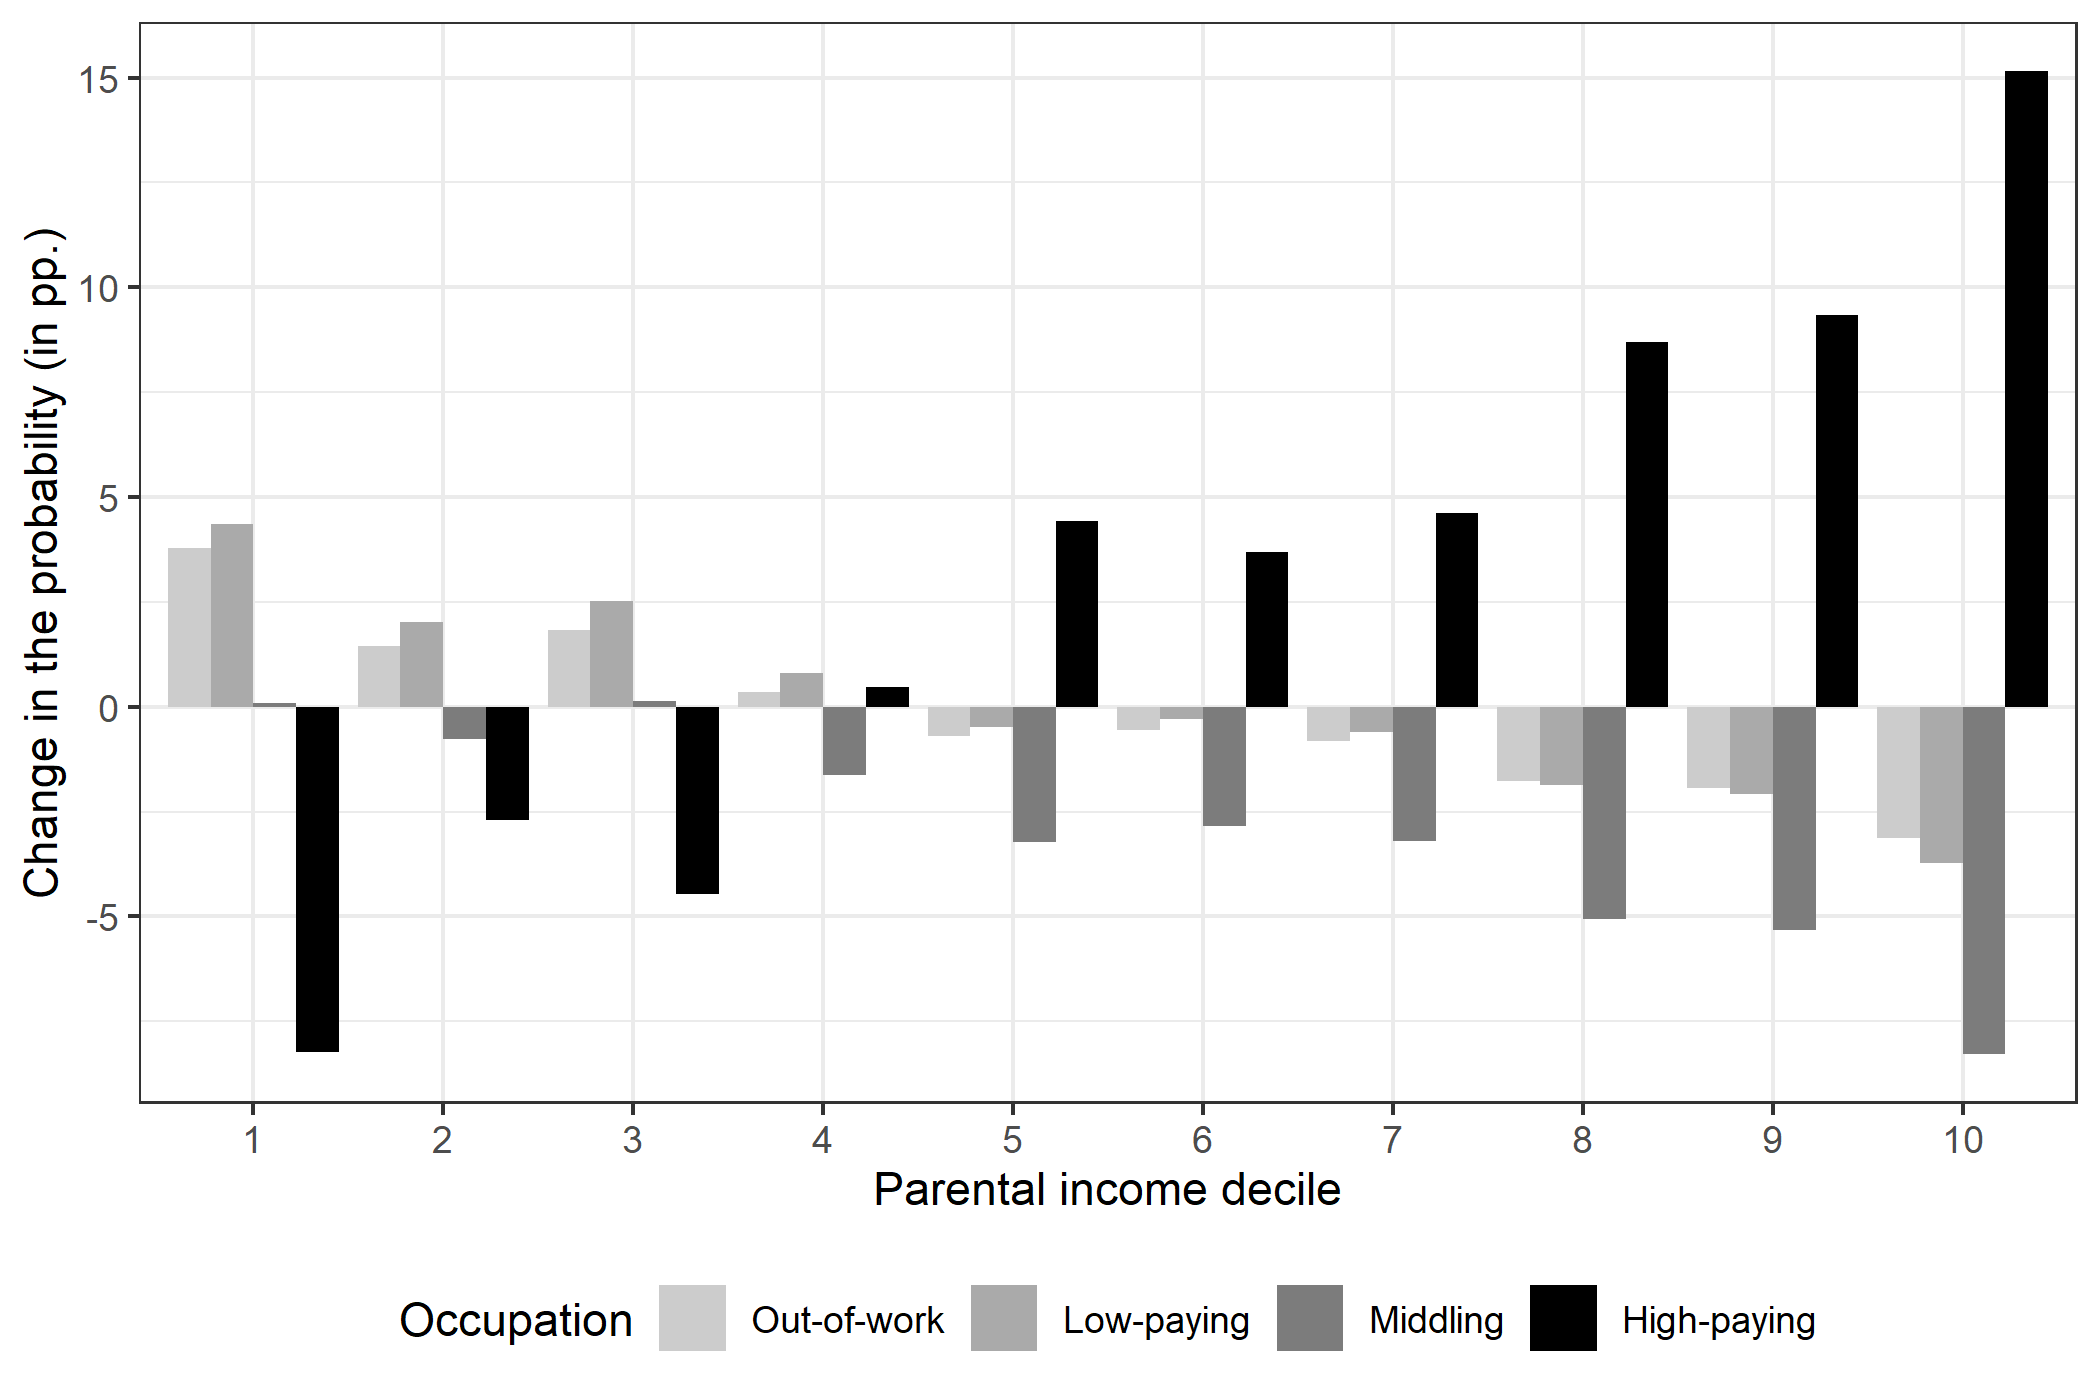
\includegraphics[width=\linewidth]{chap2/graphic/occ-multi2-quant-male.png}
 	\vspace{-3em}
 	\justify\singlespacing\footnotesize{\textit{Notes:} This figure shows the difference, expressed in percentage points, between the BCS70 and NCDS58 cohorts in terms of probability of being in each type of occupation (out-of-work, low-paying, middling, high-paying) at age 42 according to the decile of the parental income distribution. 
 	Probabilities are computed for males in both cohorts at each parental income decile, according to the multinomial logistic regression reported in columns (1) of Table \ref{chap2-tab:occ-multi23-base}.}
 \end{figure}
 
Not surprisingly, for almost all parental-income categories the likelihood of being in a middling job has declined for the younger cohort. The exception are those in the first and third deciles, for whom there has been a small increase. Yet, whether this decline is offset by an increase in the probability of working in a low- or a high-paying occupation is strongly dependent on parental income. It is only for those in the fourth decile that we see the pattern observed in the aggregate data: a reduction in the share of middling jobs accompanied by an increase in that of both low- and high-paying ones. Everywhere else in the distribution the changes in the share of high- and low-paying occupations are of opposite sign. For those in the top half of the parental-income distribution, the decline in the share of middling occupations has been accompanied by lower shares of individuals in both low-paying jobs and out of work and a higher share in high-paying occupations. The magnitude of these changes increases with parental income. For those in the top decile, the proportion of individuals in high-paying jobs rose by 15.1 pp., while that of those in middling fell by 8.3 pp. The bottom three deciles display an increase for out-of-work and low-paying and a decline for high-paying, irrespective of whether there was a positive or negative change in the share of middling jobs, though the magnitudes for the latter are small an all three cases.

Figure \ref{chap2-fig:occ-multi3-pinc-female} provides the change in the probability of being in each occupation in the second period conditional on first-period occupation at several points of the parental income distribution for females. 

\begin{figure}[!htb]
    \centering
    \caption{Change in probability to be in each occupation in the second period according to the first-period occupation and parental income (female only)}
    \label{chap2-fig:occ-multi3-pinc-female}
    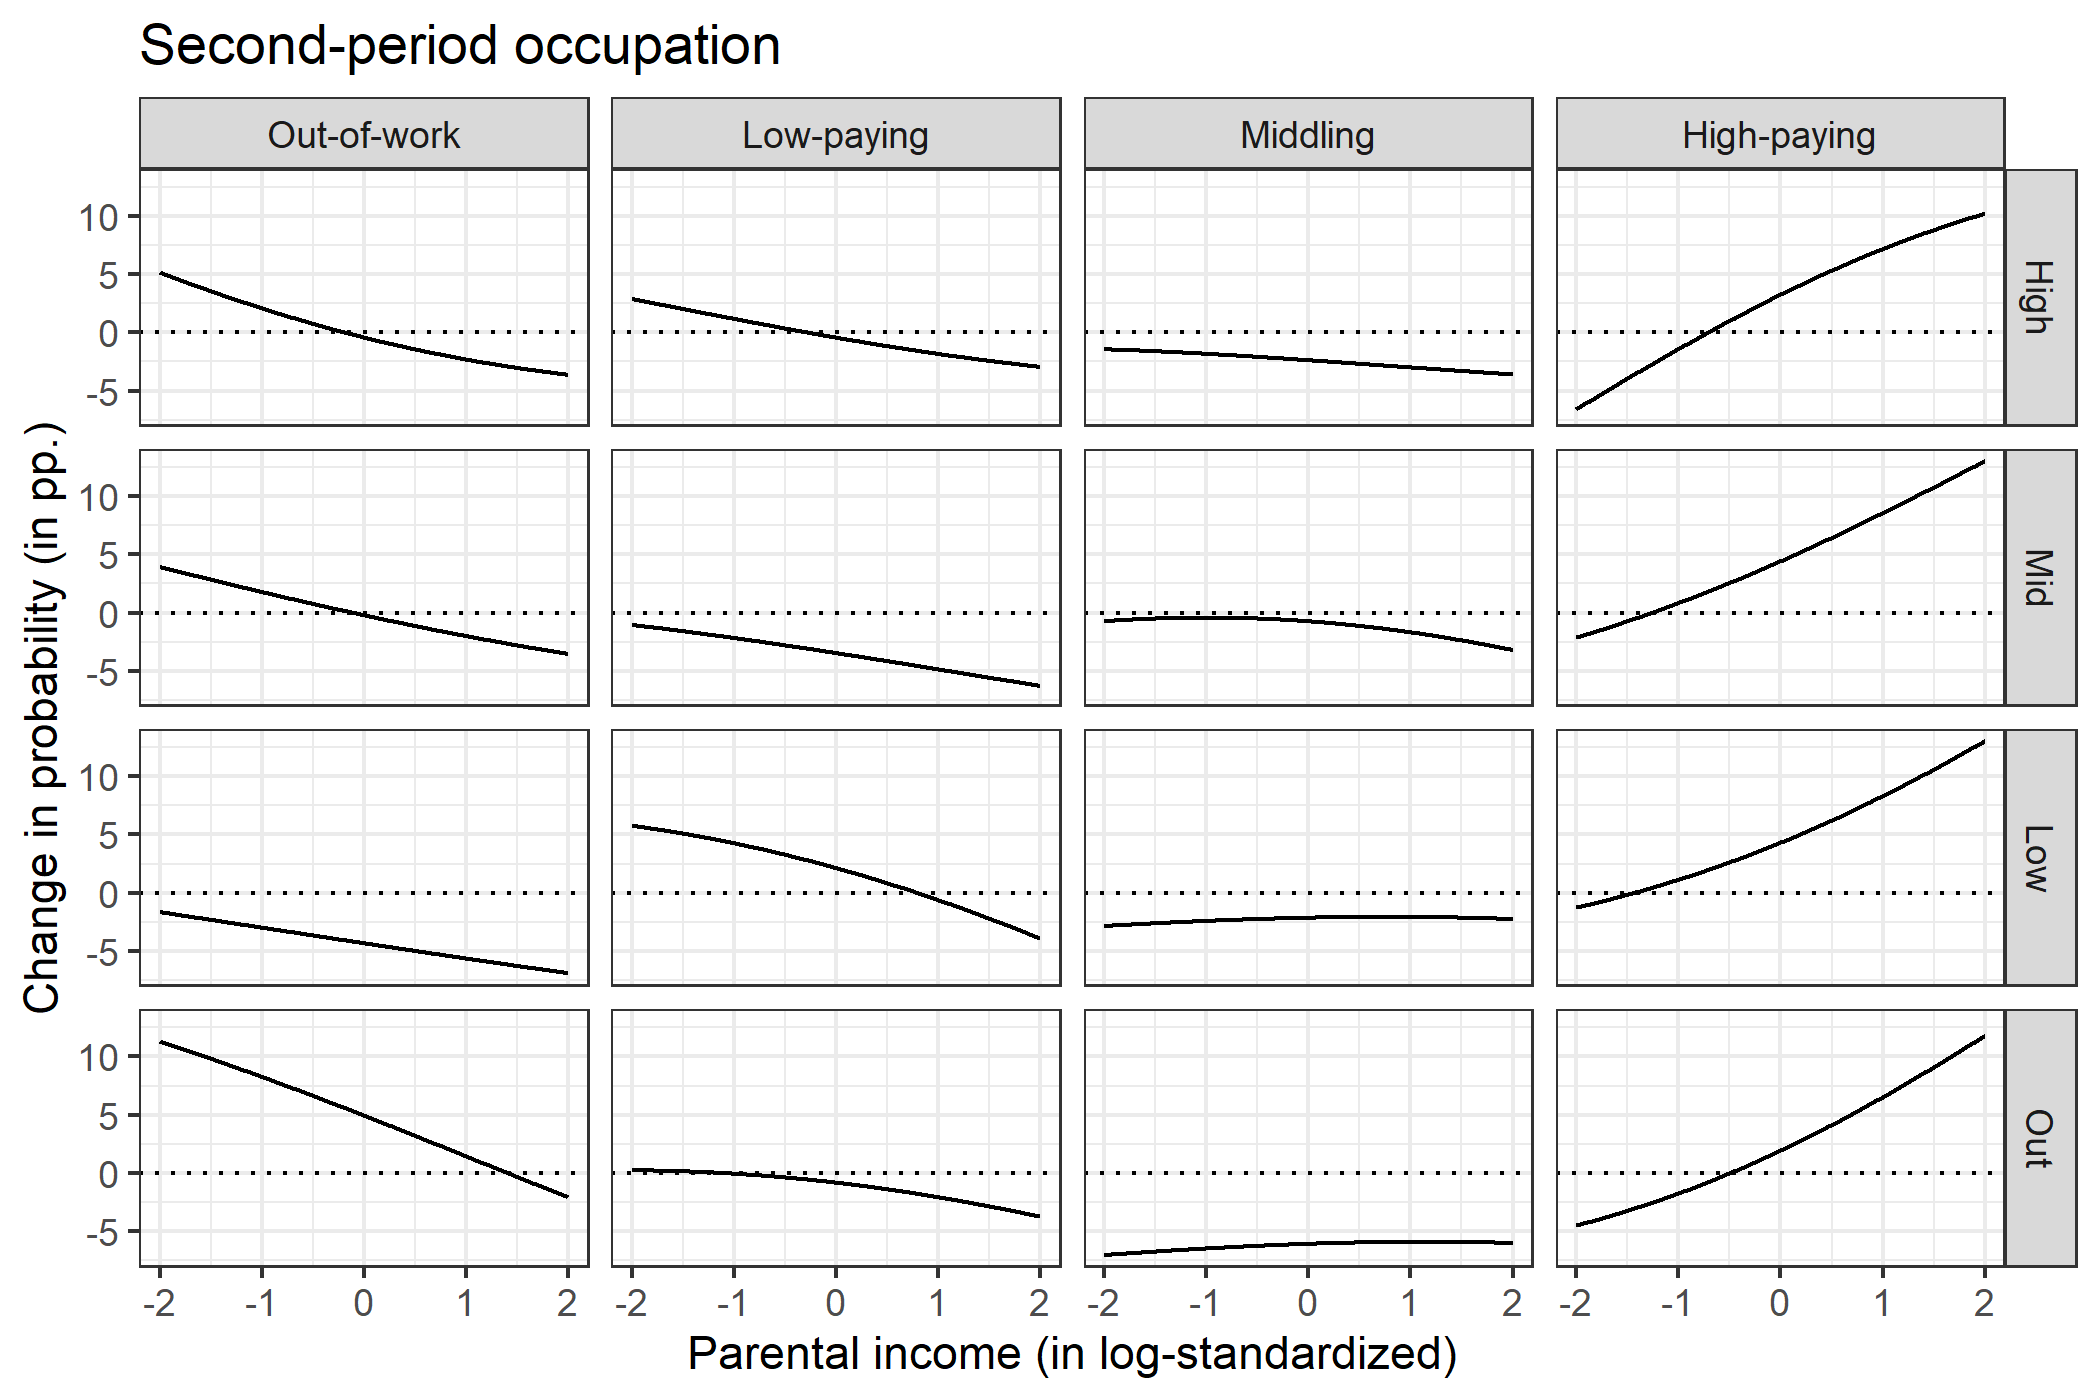
\includegraphics[width=\linewidth]{chap2/graphic/occ-multi3-pinc-female.png}
    \vspace{-3em}
    \justify\singlespacing\footnotesize{\textit{Notes:} This figure presents the difference, expressed in percentage points, between the BCS70 and the NCDS58 cohorts in terms of probability of being in each type of second-period occupation (out-of-work, low-paying, middling, high-paying), conditional on the first-period occupation, according to parental income, in log-standardized.
    Probabilities are computed for females in both cohorts according to the multinomial logistic regression reported in columns (2) of Table \ref{chap2-tab:occ-multi23-base}.}
\end{figure}

We summarize the results on transition probabilities in Table \ref{chap2-tab:mob-pinc-both}. The table reports changes in the probability of each type of mobility depending on the individual’s initial occupation, assessed at several points of the parental income distribution as in the graphs above. The left panel of the table provides the results for men, the right panel for women.
\begin{table}[!tb]
    \centering
    \caption{Change in intra-generational mobility across cohorts}
    \label{chap2-tab:mob-pinc-both}
    \begin{threeparttable}
        \setlength{\tabcolsep}{9pt}
        
\begin{tabular}{lrrrrrr}
\toprule
\multicolumn{1}{c}{} & \multicolumn{3}{c}{Male} & \multicolumn{3}{c}{Female} \\
\cmidrule(l{3pt}r{3pt}){2-4} \cmidrule(l{3pt}r{3pt}){5-7}
First-period occupation & Down & Persist & Up & Down & Persist & Up\\
\midrule
& \multicolumn{3}{c}{\textit{at +2 STD}} & \multicolumn{3}{c}{\textit{at +2 STD}}\\ 
\midrule
Out-of-work &  & -0.57 & 0.57 &  & -2.05 & 2.05\\
Low-paying & -4.41 & -0.88 & 5.29 & -6.88 & -3.90 & 10.78\\
Middling & -3.84 & -0.52 & 4.36 & -9.82 & -3.20 & 13.02\\
High-paying & -2.95 & 2.95 &  & -10.19 & 10.19 & \\
\midrule 
 & \multicolumn{3}{c}{\textit{at the Mean}} & \multicolumn{3}{c}{\textit{at the Mean}}\\ 
\midrule
Out-of-work &  & 4.92 & -4.92 &  & 4.96 & -4.96\\
Low-paying & -2.70 & 4.83 & -2.13 & -4.32 & 2.14 & 2.18\\
Middling & -0.70 & 3.65 & -2.95 & -3.68 & -0.74 & 4.42\\
High-paying & 2.54 & -2.54 &  & -3.25 & 3.25 & \\
\midrule 
 & \multicolumn{3}{c}{\textit{at -2 STD}} & \multicolumn{3}{c}{\textit{at -2 STD}}\\ 
\midrule
Out-of-work &  & 11.27 & -11.27 &  & 11.30 & -11.30\\
Low-paying & -0.53 & 9.57 & -9.04 & -1.65 & 5.76 & -4.11\\
Middling & 3.29 & 5.41 & -8.70 & 2.87 & -0.74 & -2.14\\
High-paying & 10.92 & -10.92 &  & 6.58 & -6.58 & \\
\bottomrule
\end{tabular}

            \begin{tablenotes}[flushleft]
                \footnotesize{\item \textit{Notes}: This Table summarizes the difference, expressed in percentage points, between the BCS70 and the NCDS58 cohorts in terms of type of mobility (down, persist, up) conditional on first period occupation (out-of-work, low-paying, middling, high-paying) at several points of the parental income distribution (at +2 std., at the mean, at -2 std.). These values are computed from the results obtained in Figure \ref{chap2-fig:occ-multi3-pinc-male} for males and in Figure \ref{chap2-fig:occ-multi3-pinc-female} for females.}
            \end{tablenotes}
    \end{threeparttable}
\end{table}

\subsubsection{Results at the regional level}\label{chap2-app-additional-regional}

Figures \ref{chap2-fig:reg-multi2-pinc-male} and \ref{chap2-fig:reg-multi2-pinc-female} depict the probabilities of being in each second period occupation according to parental income at the regional level, for men and women respectively. Figure  \ref{chap2-fig:regocc-absolute-all} depicts the correlation between the change in the parental income coefficient for second-period occupations and the change in job polarization at the regional level.

\begin{figure}[!htb]
    \centering
    \caption{Second-period occupation probability according to parental income at the regional level (male only)}
    \label{chap2-fig:reg-multi2-pinc-male}
    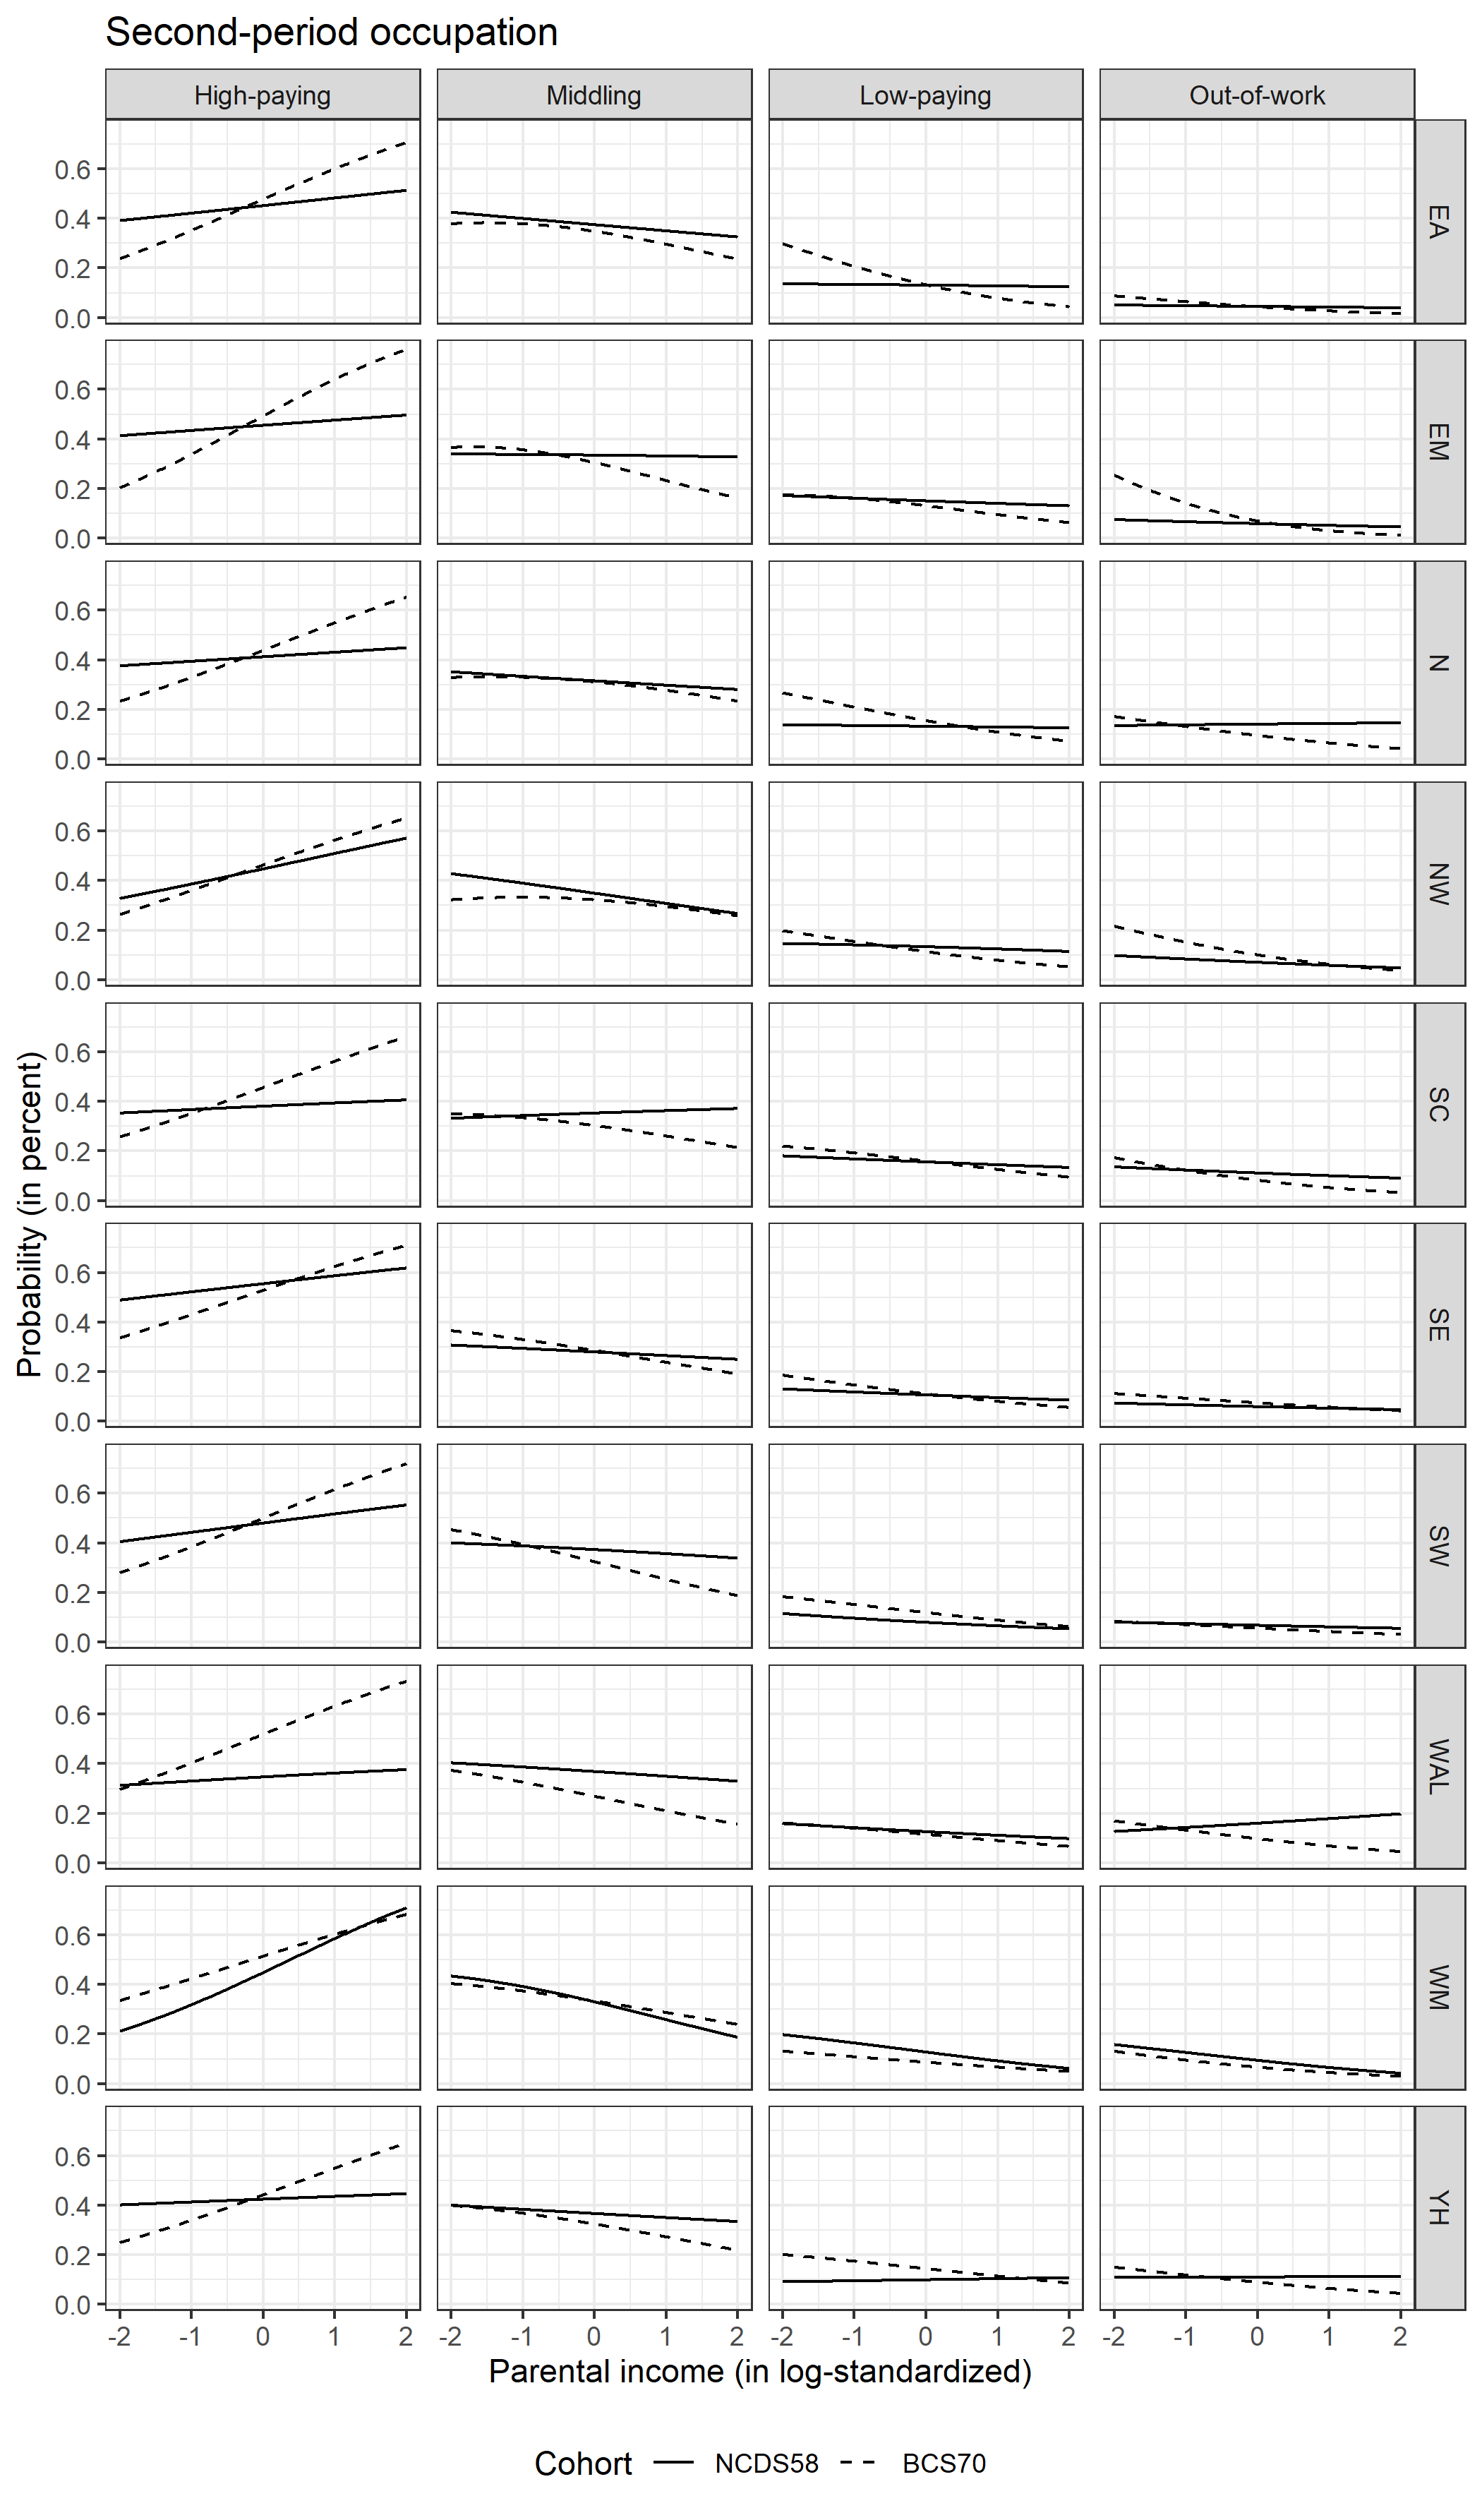
\includegraphics[width=.7\linewidth]{chap2/graphic/reg-multi2-pinc-male.png}
    \vspace{-3em}
	\justify\singlespacing\footnotesize{\textit{Notes:} This figure presents the probability, expressed in percent, of being in each type of occupation (out-of-work, low-paying, middling, high-paying) in second period according to parental income, in log-standardized, for each region.
	Probabilities are computed for males in both cohorts according to the multinomial logistic regressions reported in Table \ref{chap2-tab:reg-multi2-short}.}
\end{figure}

\begin{figure}[!htb]
    \centering
    \caption{Second-period occupation probability according to parental income at the regional level (female only)}
    \label{chap2-fig:reg-multi2-pinc-female}
    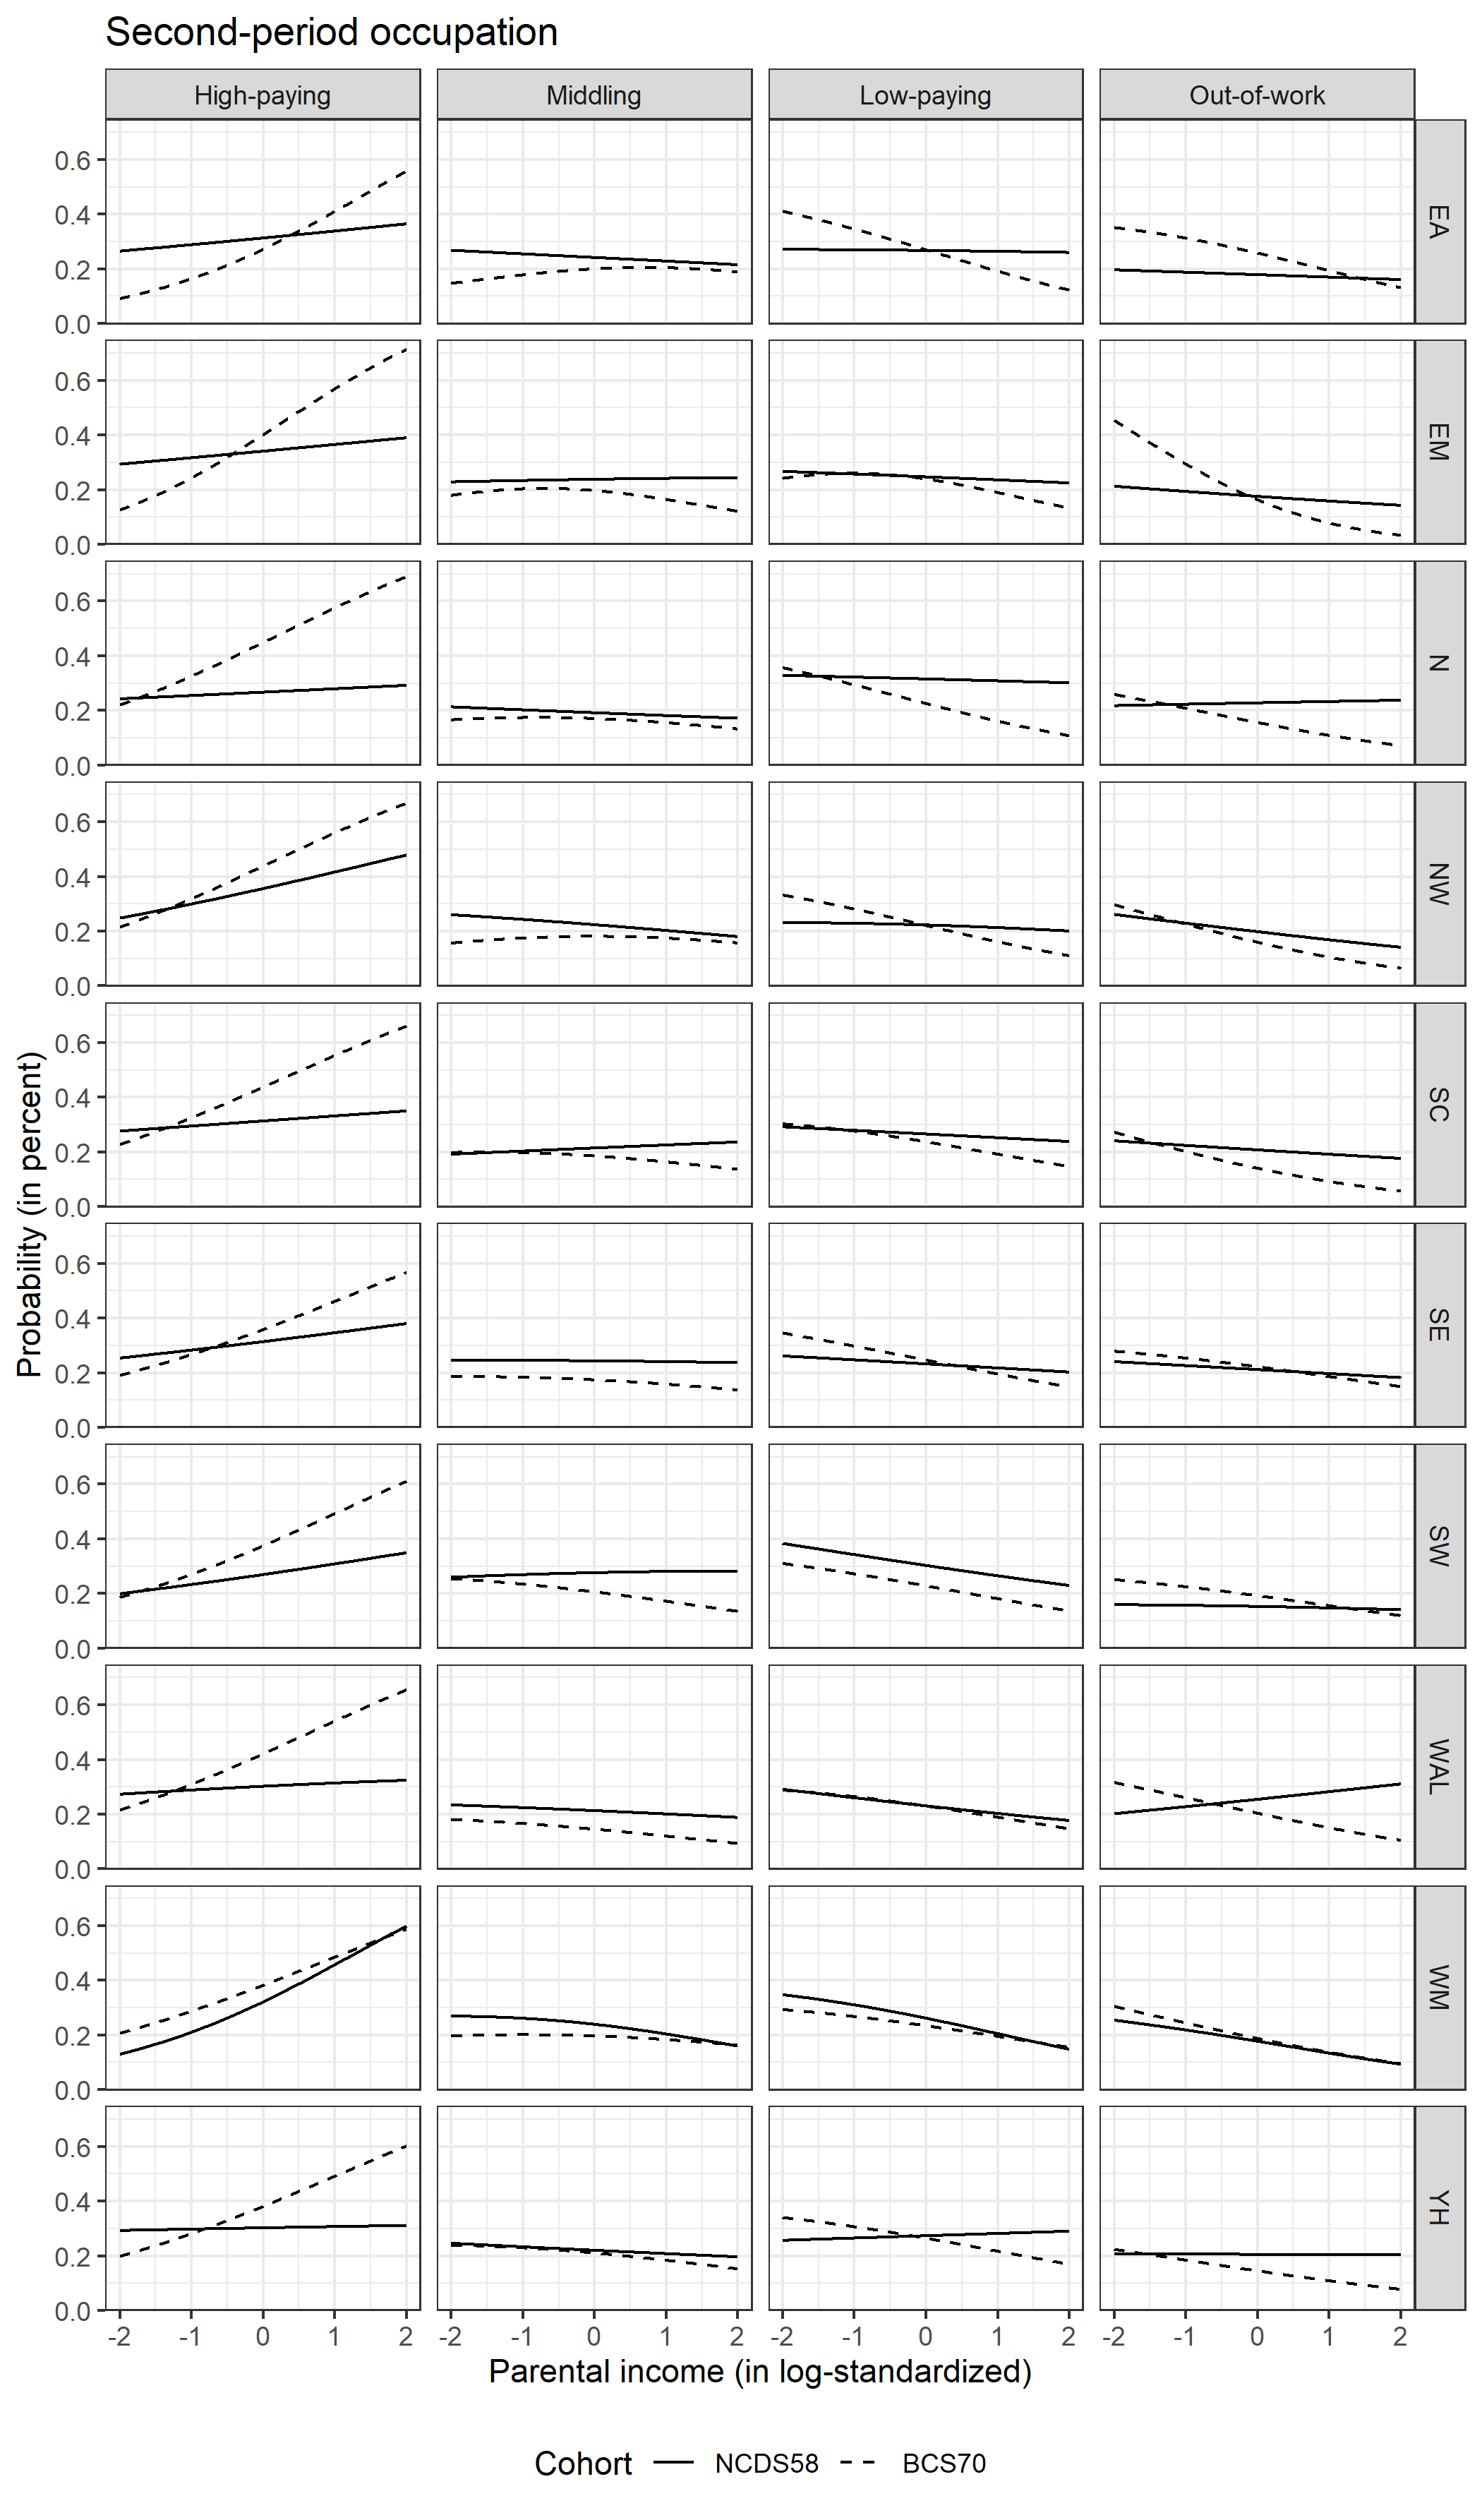
\includegraphics[width=.7\linewidth]{chap2/graphic/reg-multi2-pinc-female.png}
    \vspace{-3em}
	\justify\singlespacing\footnotesize{\textit{Notes:} This figure presents the probability, expressed in percent, of being in each type of occupation (out-of-work, low-paying, middling, high-paying) in second period according to parental income, in log-standardized, for each region.
	Probabilities are computed for females in both cohorts according to the multinomial logistic regressions reported in Table \ref{chap2-tab:reg-multi2-short}.}
\end{figure}

\begin{landscape}
\begin{table}[!tb]
    \centering
    \caption{Probability of being in each occupation in the second period according to the shares of middling and high-paying occupations in the region at the age 16 (multinomial)}
    \label{chap2-tab:regocc-multi2B-short}
    % \resizebox*{!}{\dimexpr\textheight-2\baselineskip\relax}{
    % \resizebox*{\textwidth}{!}{
    \begin{threeparttable}
        \setlength{\tabcolsep}{-1pt}
        \begin{tabular}{l D{.}{.}{5.3} D{.}{.}{5.5} D{.}{.}{5.5} D{.}{.}{5.3} D{.}{.}{5.5} D{.}{.}{5.5} D{.}{.}{5.3} D{.}{.}{5.5} D{.}{.}{5.5}}
\toprule
 & \multicolumn{9}{c}{Multinomial logit - Dep. var.: Second-period occupation} \\
\cmidrule(lr){2-10}
 & \multicolumn{3}{c}{(1)} & \multicolumn{3}{c}{(2)} & \multicolumn{3}{c}{(3)} \\
\cmidrule(lr){2-4}\cmidrule(lr){5-7}\cmidrule(lr){8-10}
 & \multicolumn{1}{c}{Low} & \multicolumn{1}{c}{Mid} & \multicolumn{1}{c}{High} & \multicolumn{1}{c}{Low} & \multicolumn{1}{c}{Mid} & \multicolumn{1}{c}{High} & \multicolumn{1}{c}{Low} & \multicolumn{1}{c}{Mid} & \multicolumn{1}{c}{High} \\
\midrule
Middling share                 & -0.07  & -0.02      & -0.17^{***} &        &            &            & 0.22   & -0.22      & -0.21       \\
                               & (0.06) & (0.05)     & (0.05)      &        &            &            & (0.34) & (0.32)     & (0.30)      \\
High-paying share              &        &            &             & 0.10   & -0.01      & 0.28^{***} & 0.37   & -0.41      & -0.25       \\
                               &        &            &             & (0.07) & (0.06)     & (0.06)     & (0.51) & (0.48)     & (0.46)      \\
Parental income                & 0.04   & 0.11^{***} & 0.35^{***}  & 0.04   & 0.11^{***} & 0.36^{***} & 0.05   & 0.12^{***} & 0.38^{***}  \\
                               & (0.03) & (0.03)     & (0.03)      & (0.03) & (0.03)     & (0.03)     & (0.03) & (0.03)     & (0.03)      \\
Par. inc. $\times$ Mid. share  & 0.00   & -0.04^{*}  & -0.11^{***} &        &            &            & -0.06  & -0.13^{**} & -0.29^{***} \\
                               & (0.03) & (0.02)     & (0.02)      &        &            &            & (0.06) & (0.05)     & (0.05)      \\
Par. inc. $\times$ High. share &        &            &             & -0.01  & 0.02       & 0.05^{**}  & -0.06  & -0.09^{*}  & -0.17^{***} \\
                               &        &            &             & (0.02) & (0.02)     & (0.02)     & (0.05) & (0.05)     & (0.05)      \\
\midrule
Num. obs. & \multicolumn{1}{c}{14763} & \multicolumn{1}{c}{14763} & \multicolumn{1}{c}{14763} & \multicolumn{1}{c}{14763} & \multicolumn{1}{c}{14763} & \multicolumn{1}{c}{14763} & \multicolumn{1}{c}{14763} & \multicolumn{1}{c}{14763} & \multicolumn{1}{c}{14763}\\
\bottomrule
\end{tabular}

        \begin{tablenotes}[flushleft]
            \footnotesize{\item\textit{Notes}: 
            % Stars and SE
            $^{***}p<0.01$; $^{**}p<0.05$; $^{*}p<0.1$. Standard errors between parentheses. 
            % Baseline outcome
            Out-of-work occupation in second period is the base outcome of the multinomial logistic regression.
            % Referent group
            Male is the referent group in all regressions.
            % Variables details
            Parental income in logarithm and then standardized at the cohort level. Middling and High-paying shares correspond to, respectively, the shares of middling and high-paying in total employment in the region at age 16. Both shares have been standardized for the interpretability of coefficients when interacted with parental income.
            % Control variables
            Control variables in (1) include Intercept, Female and Female $\times$ BCS, while control variables in (2) include Intercept, Female and Female $\times$ Non-Mid. share. %; see Table \ref{chap2-tab:tobefilled} in the appendix for these coefficients.
            }
        \end{tablenotes}
    \end{threeparttable}
    % }}
\end{table}
\end{landscape}

\begin{figure}[!tb]
    \centering
    \caption{Change in parental income coefficient for second-period occupation according to job polarization at the regional level}
    \label{chap2-fig:regocc-absolute-all}
    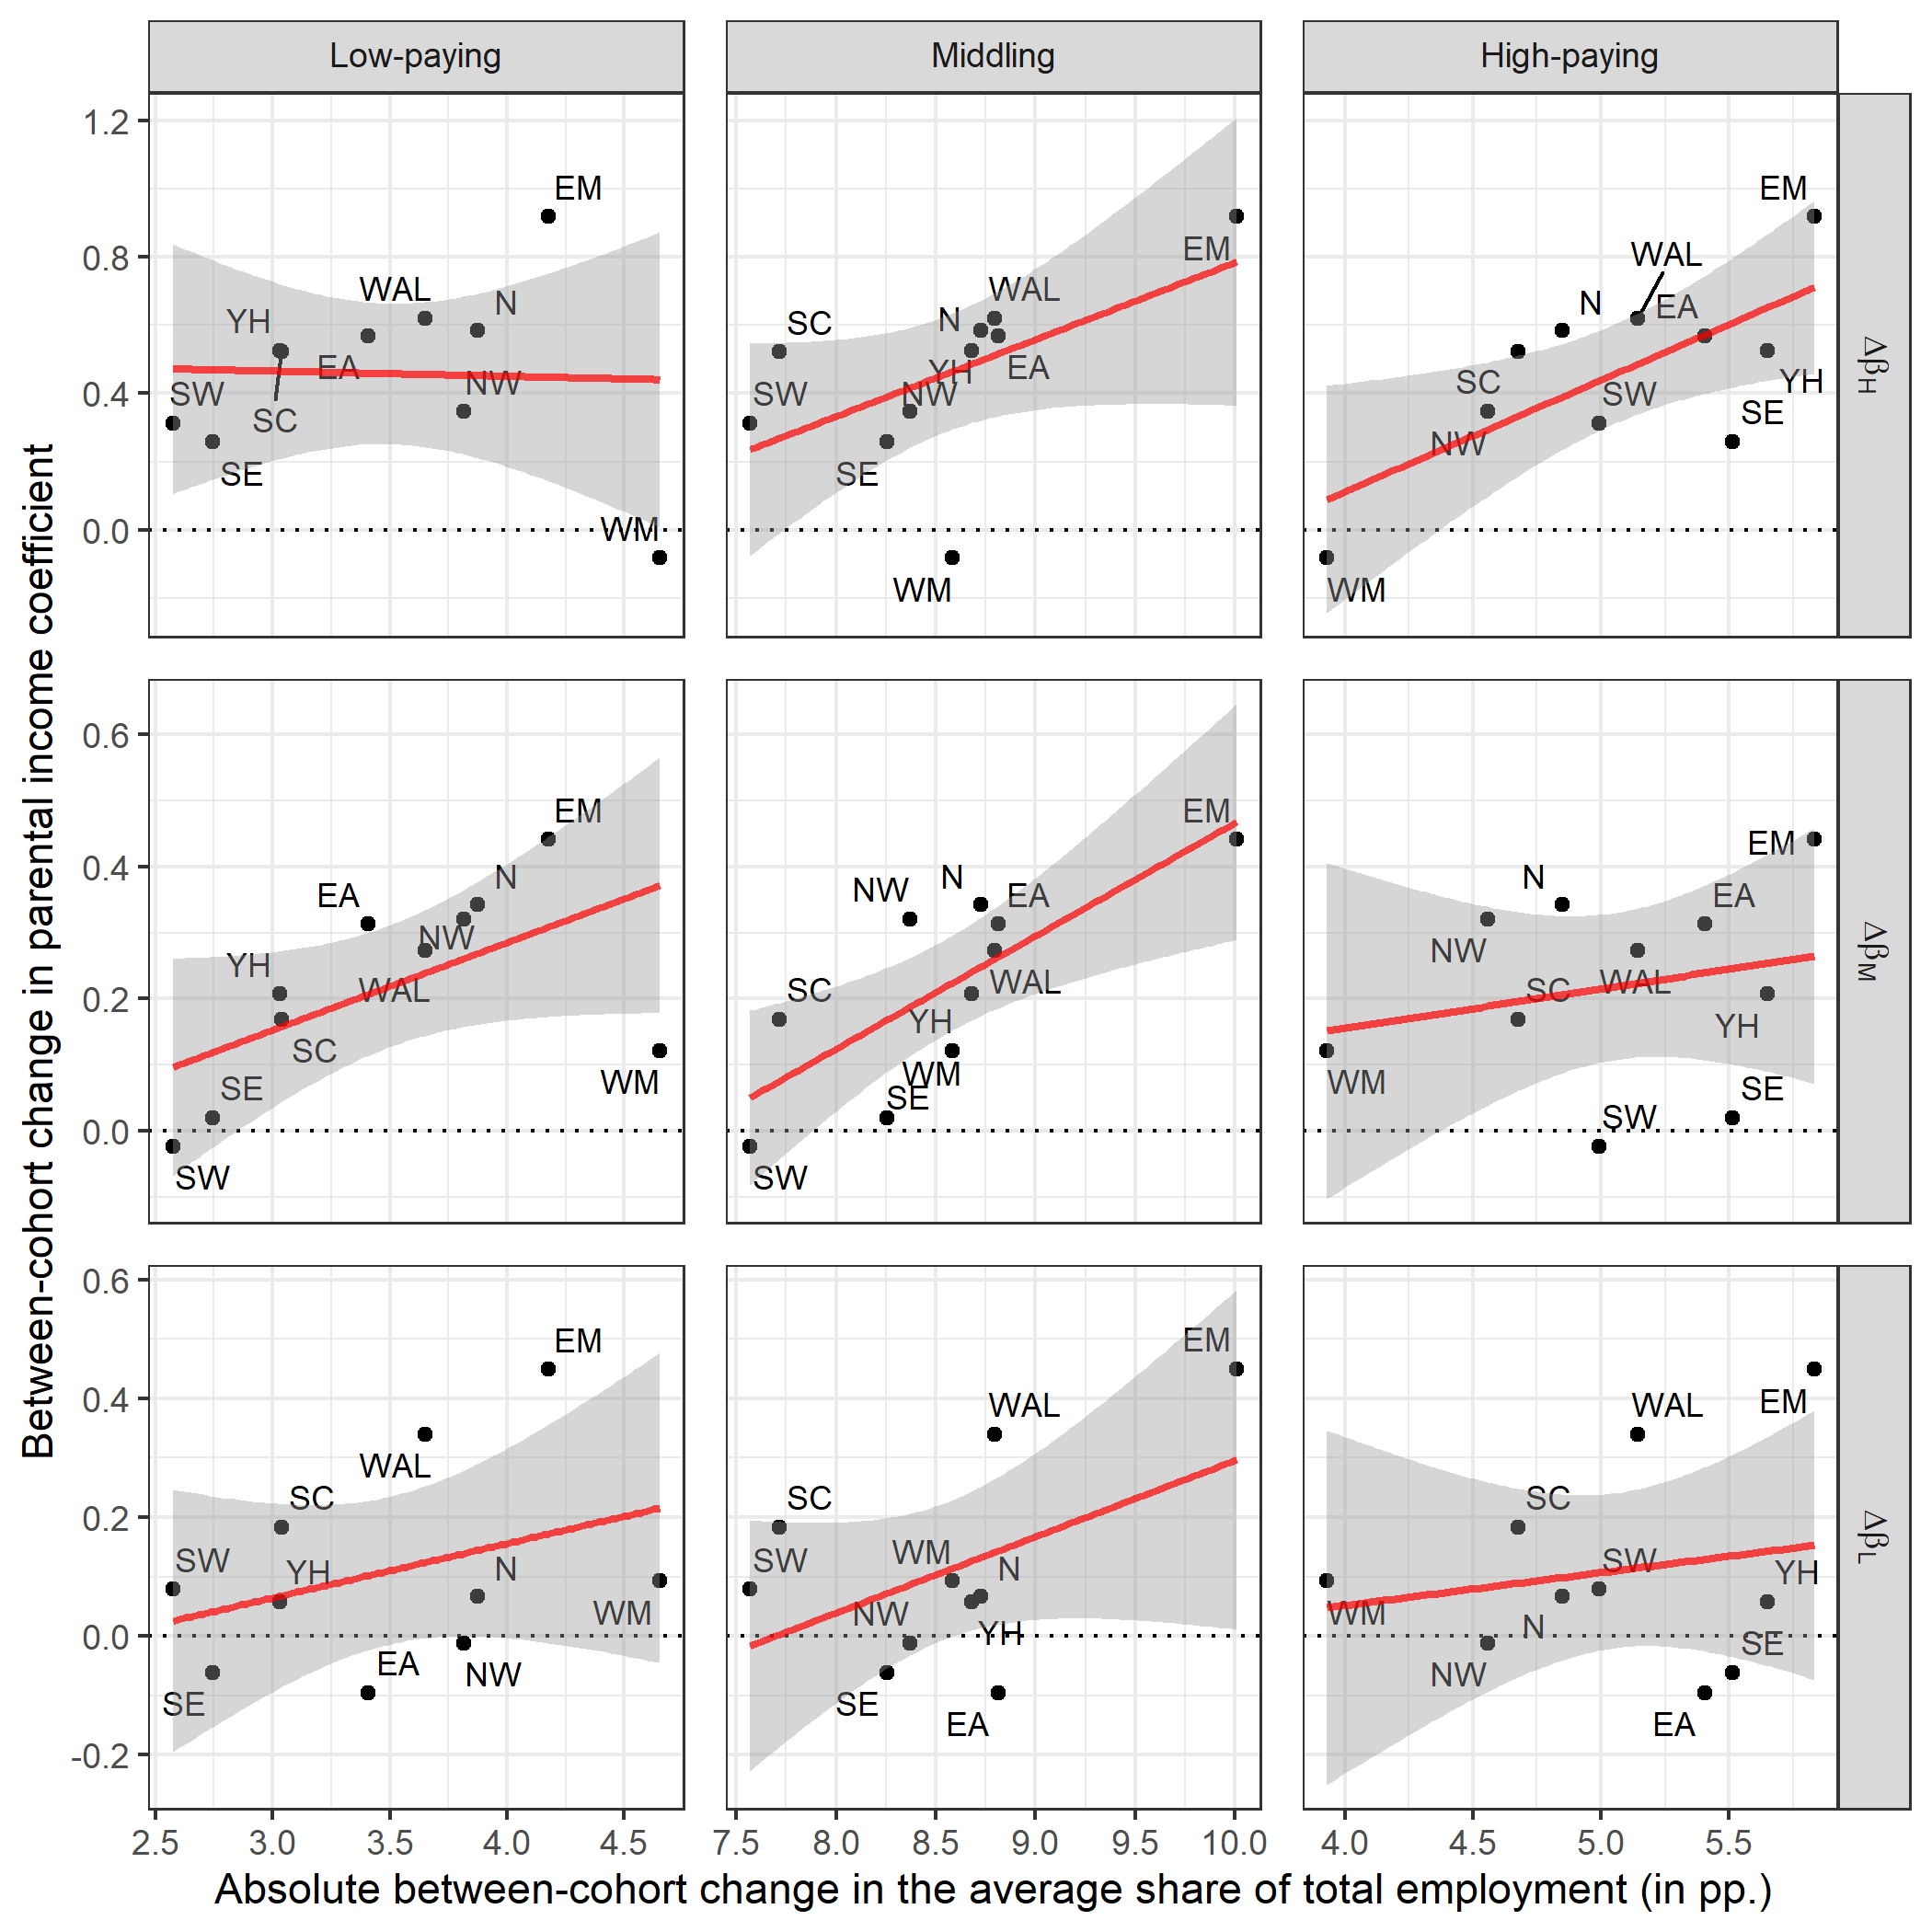
\includegraphics[width=\linewidth]{chap2/graphic/regocc-absolute-all.png}
    \vspace{-3em}
	\justify\singlespacing\footnotesize{\textit{Notes:} This figure presents the correlation across regions between the change in the parental income coefficient for each occupation (low-paying, middling, and high-paying) in second period $\Delta\beta_k$ and the between-cohort change in absolute value in the average share of total employment of low-paying, middling, and high-paying occupations, in percentage points. Note that, by taking the absolute value of the change, we reversed the x-axis for the middling panels (middle column). Thus, regions on the left-hand (resp. right-hand) side of each panel are those where the polarization of employment has been lower (resp. larger).}
\end{figure}
    \clearpage
    \subsection{Decomposing the effect of parental income}\label{chap2-app-decomposing}
    %\subsubsection{Decomposing the effect of parental income} \label{chap2-trade-off}

This appendix examines how the effect of parental income on the occupations of mature workers operates through its impact on both first and second period occupations. Our results indicate that, conditional on first period occupation, the role of parental income in determining occupational outcomes has increased. At the same time, as is clear from the regressions, initial occupations are also important to determine outcomes at age 42. In particular, those who started their careers in middling have a probability to move to high-paying occupations that is about 7 pp. higher than those who started in a low-paying occupation (see Table \ref{chap2-tab:proba-group5-cdt-short}). Similarly, entering the labour market in a middling occupation implies a likelihood to be in such an occupation at age 42 at least 20 pp. higher than entering in a low-paying job. We would hence like to assess to what extent parental income compensates for past occupations. 

We compare the probability to be in a middling occupation at age 42 for two individuals who started in different initial occupations, middling and low-paying, and compute the additional parental income that the latter would need to have in order to compensate the advantage given by starting work in a middling occupation. To do so, we define the ratio between the two probabilities
\begin{equation}\label{chap2-eq:relative-proba}
    \frac{p_{M}^{M}}{p_{M}^{L}} = \frac{p_O^M}{p_O^L}\exp\Big(\eta_{MM} -\eta_{ML} + \beta_{3M} (Y^M-Y^L)\Big),
\end{equation}
where $p^j_k$ is the probability of being in occupation $k$ in second period conditional on having started in occupation $j$, and $Y^L$ and $Y^M$ are, respectively, the parental income of the individual starting in a low-paying occupation and of that starting in a middling occupation. 

For both cohorts, we derive the parental income $Y^c=Y^L-Y^M$ such that the two individuals are as likely to be in a middling occupation at age 42, i.e. $p_{M}^{M}=p_{M}^{L}$. Thus,
\begin{equation}\label{chap2-eq:counter-Y}
    Y^c \equiv \frac{\eta^c}{\beta^c} = \frac{\eta^c_{MM} -\eta^c_{ML} - \log(p_O^M/p_O^L)}{\beta^c_{3M}},
\end{equation}
where $p_O^M$ and $p_O^L$ are evaluated at the mean of the parental income distribution. We interpret $Y^c$ as the additional parental income that an individual in cohort $c$ starting in occupation $L$ needs in order to be as likely as one starting in occupation $M$ to be in a middling occupation when mature.
Thus, $\eta^c$ captures the degree of persistence in $M$, whereas $\beta^c$ reflects the effectiveness of parental income in moving into a middling occupation in second period. The greater the degree of persistence in $M$, the greater the parental income required to compensate the advantage given by the first-period occupation, i.e. $\partial Y^c/\partial\eta^c > 0$. The greater the effectiveness of parental income, the smaller the parental income required to compensate, i.e. $\partial Y^c/\partial\beta^c < 0~\forall\Delta\beta > 0$.

This difference in parental income reflects the value conferred by being in a certain first-period occupation---compared to parental income---for mobility across occupations. Taking the ratio between $Y^{70}$ and $Y^{58}$, we obtain the \emph{change across cohorts in the relative advantage} such that
\begin{equation}\label{chap2-eq:delta-Y}
    \Delta Y \equiv \frac{Y^{70}}{Y^{58}}= \frac{\Delta\eta}{\Delta\beta}
\end{equation}
where $\Delta\eta = \eta^{70}/\eta^{58}$ captures the effect of the change in the degree of persistence and $\Delta\beta = \beta^{70}/\beta^{58}$ reflects the effect of the change in the role of parental income. 
Both affect the worth of the first-period occupation in opposite ways.
%\footnote{ 
The greater the change in the degree of persistence, the greater the change in parental income needed to compensate, hence, the greater the relative worth of first-period occupation, i.e. $\partial\Delta Y/\partial\Delta\eta > 0$.
The greater the change in the effectiveness of parental income, the smaller the change in the parental income to compensate, hence, the smaller the relative worth of first-period occupation, i.e. $\partial\Delta Y/\partial\Delta\beta < 0~\forall\Delta\beta > 0$.
%}

Table \ref{chap2-tab:decomp-all} presents the decomposition of the relative advantage of first-period occupation---compared to parental income---for upward mobility.
\begin{table}[!tb]
    \centering
    \caption{Relative advantage of the first-period occupation with respect to parental income}
    \label{chap2-tab:decomp-all}
    \begin{threeparttable}
        \setlength{\tabcolsep}{9pt}
        
\begin{tabular}{lrrrrrrrrr}
\toprule
\multicolumn{1}{c}{} & \multicolumn{3}{c}{$p_{M}^{M}=p_{M}^{L}$} & \multicolumn{3}{c}{$p_{H}^{H}=p_{H}^{M}$} & \multicolumn{3}{c}{$p_{H}^{H}=p_{H}^{L}$} \\
\cmidrule(l{3pt}r{3pt}){2-4} \cmidrule(l{3pt}r{3pt}){5-7} \cmidrule(l{3pt}r{3pt}){8-10}
  & \multicolumn{1}{c}{$Y$} & \multicolumn{1}{c}{$\eta$} & \multicolumn{1}{c}{$\beta$} & \multicolumn{1}{c}{$Y$} & \multicolumn{1}{c}{$\eta$} & \multicolumn{1}{c}{$\beta$} & \multicolumn{1}{c}{$Y$} & \multicolumn{1}{c}{$\eta$} & \multicolumn{1}{c}{$\beta$}\\
\midrule
BCS70 & 4.63 & 0.73 & 0.16 & 2.13 & 0.84 & 0.39 & 2.25 & 0.89 & 0.39\\
NCDS58 & 13.11 & 0.60 & 0.05 & 5.47 & 0.79 & 0.14 & 6.24 & 0.90 & 0.14\\
\midrule
$\Delta$ & 0.35 & 1.22 & 3.45 & 0.39 & 1.07 & 2.74 & 0.36 & 0.99 & 2.74\\
\midrule
$\Delta$ ($\eta$ constant) & 0.29 & 1.00 & 3.45 & 0.37 & 1.00 & 2.74 & 0.37 & 1.00 & 2.74\\
$\Delta$ ($\beta$ constant) & 1.22 & 1.22 & 1.00 & 1.07 & 1.07 & 1.00 & 0.99 & 0.99 & 1.00\\
\bottomrule
\end{tabular}

        \begin{tablenotes}[flushleft]
            \footnotesize{\item\textit{Notes}: This table presents the relative advantage of the first-period occupation with respect to parental income for upward mobility. 
            $Y$ corresponds to the parental income that an individual in cohort $c$ needs in order to compensate for having started one occupational category below, $\eta$ captures the degree of persistence, whereas $\beta$ captures the effectiveness of parental income. 
            Coefficients for the NCDS58 and BCS70 cohorts are computed for males using Table \ref{chap2-tab:occ-multi23-base} in the appendix.
            $\Delta$ rows refer to the ratio between the BCS70 and NCDS58 under three specifications: the actual ratio, the ratio keeping $\eta$ constant, and the ratio keeping $\beta$ constant.}
        \end{tablenotes}
    \end{threeparttable}
\end{table}
We consider three cases: the difference in reaching a middling occupation for those starting in low-paying or in middling occupations (left panel), the difference in reaching a high-paying occupation for those starting in high-paying or in middling occupations (middle panel), and the difference in reaching a high-paying occupation for those starting in low-paying or in high-paying occupations (right panel). 

% BUT recall that parental income was ABSOLUTELY less important to determine first-period occ. in the NCDS58. Also eta has increased so the ABSOLUTE value of initial occupation has increased 

Consider first the relative effect of initial occupations versus parental income for the NCDS58. Because parental income is standardized, the figures reported for $Y^{70}$ represent the standard deviations needed to compensate the difference when starting in the various initial occupations (computed at the mean of parental income.). For the three cases we report, the additional income required is between 5.47 and 13.11 standard deviations. Such large magnitudes imply that it was hard for parental income to compensate the advantage conferred by a more favourable initial occupation, and, in the case of the probabilities of being in a middling occupation at age 42 ($p_M^M$  and $p_M^L$, left panel) only a massive difference in parental income could compensate the advantage that being in a middling occupation at 23 conferred. When we compare these figures with those for the BCS70, we can see that the additional income required to compensate the most favourable occupation is between 2.13 and 4.63 standard deviations, magnitudes that amount to about a third of those needed for the older cohort. 

The bottom two lines allow us to understand what is driving this change. We compute the ratio $Y^{70}/Y^{58}$ by keeping constant, i.e. at the value it had for the NCDS58, either $\eta$ or $\beta$. Recall from equation (5) that $\eta$ captures the degree of persistence in an occupation, whereas $\beta$ reflects the advantage to move upwards conferred by parental income. The three cases we examine display the same pattern. When we keep $\eta$ constant we obtain a change in the relative importance of parental income that is very close to the actual one, indicating that changes in persistence have played a minor role. In contrast, keeping $\beta$ constant results in values of $\Delta Y$ that are around or above 1. That is, what is driving the differences across cohorts in the advantage that parental income affords relative to initial occupations is the direct effect of the former rather than any changes in persistence associated with the latter.

These results indicate that there has been a major change in the relative roles that entry jobs and parental background play in determining the occupational outcomes of mature individuals. For the older cohort, the advantage conferred by entry occupations could only be offset by vast amounts of parental income; for the younger one, the latter has become much more able to offset the career advantages conferred by early career experiences.

    \clearpage
    \subsection{Robustness checks}\label{chap2-app-robustness}
    \subsubsection{Squared parental income}

This appendix provides a robustness check on the role of squared parental income. We consider the non-logarithmic parental income although standardized.
Table \ref{chap2-tab:rob1-multi1-base} shows the coefficients of the multinomial logistic regression for the probability of being in each first-period occupation.
Table \ref{chap2-tab:rob1-multi2-base} shows the coefficients of the multinomial logistic regression for the probability of being in each second-period occupation.
Table \ref{chap2-tab:rob1-multi3-base} shows the coefficients of the multinomial logistic regression for the probability of being in each second-period occupation according to first-period occupation.

\begin{table}[!htb]
    \centering
    \caption{Probability of being in each occupation in first period (Squared-parental-income robustness check)}
    \label{chap2-tab:rob1-multi1-base}
    \resizebox{\textwidth}{!}{
    \begin{threeparttable}
        \setlength{\tabcolsep}{0pt}
        \begin{tabular}{l D{.}{.}{5.5} D{.}{.}{5.5} D{.}{.}{5.5} D{.}{.}{5.5} D{.}{.}{5.5} D{.}{.}{5.5}}
\toprule
 & \multicolumn{6}{c}{Multinomial logit - Dep. var.: First-period occupation} \\
\cmidrule(lr){2-7}
 & \multicolumn{3}{c}{(1)} & \multicolumn{3}{c}{(2)} \\
\cmidrule(lr){2-4}\cmidrule(lr){5-7}
 & \multicolumn{1}{c}{Low} & \multicolumn{1}{c}{Mid} & \multicolumn{1}{c}{High} & \multicolumn{1}{c}{Low} & \multicolumn{1}{c}{Mid} & \multicolumn{1}{c}{High} \\
\midrule
Intercept                  & 0.08        & 1.39^{***}  & 0.69^{***}  & 0.06        & 1.38^{***}  & 0.66^{***}  \\
                           & (0.07)      & (0.06)      & (0.06)      & (0.07)      & (0.06)      & (0.06)      \\
BCS cohort                 & 0.23^{**}   & 0.12        & 0.76^{***}  & 0.29^{***}  & 0.25^{***}  & 0.90^{***}  \\
                           & (0.10)      & (0.08)      & (0.09)      & (0.11)      & (0.09)      & (0.09)      \\
Female                     & -0.79^{***} & -1.27^{***} & -1.00^{***} & -0.79^{***} & -1.27^{***} & -1.00^{***} \\
                           & (0.09)      & (0.07)      & (0.08)      & (0.09)      & (0.07)      & (0.08)      \\
Female $\times$ BCS        & 0.25^{**}   & -0.01       & -0.07       & 0.25^{**}   & -0.02       & -0.07       \\
                           & (0.12)      & (0.10)      & (0.11)      & (0.12)      & (0.10)      & (0.11)      \\
Par. inc.                  & -0.03       & 0.02        & 0.28^{***}  & -0.04       & 0.02        & 0.26^{***}  \\
                           & (0.04)      & (0.03)      & (0.04)      & (0.04)      & (0.03)      & (0.04)      \\
Par. inc. $\times$ BCS     & 0.09        & 0.20^{***}  & 0.35^{***}  & 0.11        & 0.28^{***}  & 0.46^{***}  \\
                           & (0.06)      & (0.05)      & (0.05)      & (0.07)      & (0.06)      & (0.06)      \\
Par. inc.$^2$              &             &             &             & 0.02        & 0.01        & 0.03        \\
                           &             &             &             & (0.03)      & (0.02)      & (0.02)      \\
Par. inc.$^2$ $\times$ BCS &             &             &             & -0.06       & -0.14^{***} & -0.15^{***} \\
                           &             &             &             & (0.04)      & (0.03)      & (0.03)      \\
\midrule
Num. obs. & \multicolumn{1}{c}{14763} & \multicolumn{1}{c}{14763} & \multicolumn{1}{c}{14763} & \multicolumn{1}{c}{14763} & \multicolumn{1}{c}{14763} & \multicolumn{1}{c}{14763}\\
\bottomrule
\end{tabular}

        \begin{tablenotes}[flushleft]
            \footnotesize{\item\textit{Notes}:
            % Stars and SE
            $^{***}p<0.01$; $^{**}p<0.05$; $^{*}p<0.1$. Standard errors between parentheses. 
            % Referent group
            Male in the NCDS58 cohort is the referent group. 
            % Variables details
            Parental income is standardized at the cohort level and squared parental-income is the square of the standardized parental income.}
        \end{tablenotes}
    \end{threeparttable}
    }
\end{table}

\begin{table}[!htb]
    \centering
    \caption{Probability of being in each occupation in second period (Squared-parental-income robustness check)}
    \label{chap2-tab:rob1-multi2-base}
    \resizebox{\textwidth}{!}{
    \begin{threeparttable}
        \setlength{\tabcolsep}{0pt}
        \begin{tabular}{l D{.}{.}{5.5} D{.}{.}{5.5} D{.}{.}{5.5} D{.}{.}{5.5} D{.}{.}{5.5} D{.}{.}{5.5}}
\toprule
 & \multicolumn{6}{c}{Multinomial logit - Dep. var.: Second-period occupation} \\
\cmidrule(lr){2-7}
 & \multicolumn{3}{c}{(1)} & \multicolumn{3}{c}{(2)} \\
\cmidrule(lr){2-4}\cmidrule(lr){5-7}
 & \multicolumn{1}{c}{Low} & \multicolumn{1}{c}{Mid} & \multicolumn{1}{c}{High} & \multicolumn{1}{c}{Low} & \multicolumn{1}{c}{Mid} & \multicolumn{1}{c}{High} \\
\midrule
Intercept                  & 0.37^{***} & 1.37^{***}  & 1.69^{***}  & 0.45^{***}  & 1.46^{***}  & 1.72^{***}  \\
                           & (0.08)     & (0.07)      & (0.07)      & (0.08)      & (0.07)      & (0.07)      \\
BCS cohort                 & 0.03       & -0.05       & 0.11        & 0.06        & 0.03        & 0.22^{**}   \\
                           & (0.11)     & (0.09)      & (0.09)      & (0.12)      & (0.10)      & (0.10)      \\
Female                     & -0.13      & -1.22^{***} & -1.24^{***} & -0.12       & -1.22^{***} & -1.24^{***} \\
                           & (0.09)     & (0.08)      & (0.08)      & (0.09)      & (0.08)      & (0.08)      \\
Female $\times$ BCS        & -0.04      & -0.12       & 0.17        & -0.05       & -0.13       & 0.17        \\
                           & (0.13)     & (0.12)      & (0.11)      & (0.13)      & (0.12)      & (0.11)      \\
Par. inc.                  & -0.02      & 0.02        & 0.25^{***}  & -0.01       & 0.03        & 0.25^{***}  \\
                           & (0.04)     & (0.04)      & (0.04)      & (0.04)      & (0.04)      & (0.04)      \\
Par. inc. $\times$ BCS     & 0.03       & 0.12^{**}   & 0.28^{***}  & 0.09        & 0.22^{***}  & 0.39^{***}  \\
                           & (0.06)     & (0.06)      & (0.06)      & (0.07)      & (0.06)      & (0.06)      \\
Par. inc.$^2$              &            &             &             & -0.08^{***} & -0.09^{***} & -0.02       \\
                           &            &             &             & (0.03)      & (0.03)      & (0.02)      \\
Par. inc.$^2$ $\times$ BCS &            &             &             & -0.02       & -0.07^{*}   & -0.11^{***} \\
                           &            &             &             & (0.04)      & (0.04)      & (0.03)      \\
\midrule
Num. obs. & \multicolumn{1}{c}{14763} & \multicolumn{1}{c}{14763} & \multicolumn{1}{c}{14763} & \multicolumn{1}{c}{14763} & \multicolumn{1}{c}{14763} & \multicolumn{1}{c}{14763}\\
\bottomrule
\end{tabular}

        \begin{tablenotes}[flushleft]
            \footnotesize{\item\textit{Notes}: 
            % Stars and SE
            $^{***}p<0.01$; $^{**}p<0.05$; $^{*}p<0.1$. Standard errors between parentheses. 
            % Referent group
            Male in the NCDS58 cohort in out-of-work occupation in first period is the referent group. 
            % Variables details
            Parental income is standardized at the cohort level and squared parental-income is the square of the standardized parental income.
            % Explaining bottom panels
            Coefficients in the first bottom panel captures the change in the marginal effect of the first-period occupation with respect to the referent one, i.e. out-of-work. 
            Coefficients in the second bottom panel indicates the change across cohorts in the marginal effect of the first-period occupation.}
        \end{tablenotes}
    \end{threeparttable}
    }
\end{table}

\begin{table}[!htb]
    \centering
    \caption{Probability of being in each occupation in second period (Squared-parental-income robustness check)}
    \label{chap2-tab:rob1-multi3-base}
    \resizebox{\textwidth}{!}{
    \begin{threeparttable}
        \setlength{\tabcolsep}{0pt}
        \begin{tabular}{l D{.}{.}{5.5} D{.}{.}{5.5} D{.}{.}{5.5} D{.}{.}{5.5} D{.}{.}{5.5} D{.}{.}{5.5}}
\toprule
 & \multicolumn{6}{c}{Multinomial logit - Dep. var.: Second-period occupation} \\
\cmidrule(lr){2-7}
 & \multicolumn{3}{c}{(1)} & \multicolumn{3}{c}{(2)} \\
\cmidrule(lr){2-4}\cmidrule(lr){5-7}
 & \multicolumn{1}{c}{Low} & \multicolumn{1}{c}{Mid} & \multicolumn{1}{c}{High} & \multicolumn{1}{c}{Low} & \multicolumn{1}{c}{Mid} & \multicolumn{1}{c}{High} \\
\midrule
Intercept                                                                          & -0.10      & 0.44^{***}  & 0.82^{***}  & -0.03       & 0.52^{***}  & 0.85^{***}  \\
                                                                                   & (0.11)     & (0.10)      & (0.10)      & (0.11)      & (0.11)      & (0.10)      \\
BCS cohort                                                                         & -0.09      & -0.49^{***} & -0.34^{**}  & -0.05       & -0.42^{***} & -0.25^{*}   \\
                                                                                   & (0.15)     & (0.15)      & (0.14)      & (0.16)      & (0.15)      & (0.14)      \\
Female                                                                             & -0.01      & -0.98^{***} & -1.14^{***} & -0.00       & -0.98^{***} & -1.14^{***} \\
                                                                                   & (0.10)     & (0.09)      & (0.09)      & (0.10)      & (0.09)      & (0.09)      \\
Female $\times$ BCS                                                                & -0.10      & -0.09       & 0.27^{**}   & -0.11       & -0.10       & 0.26^{**}   \\
                                                                                   & (0.13)     & (0.12)      & (0.12)      & (0.13)      & (0.12)      & (0.12)      \\
Par. inc.                                                                          & -0.01      & 0.02        & 0.19^{***}  & 0.01        & 0.04        & 0.19^{***}  \\
                                                                                   & (0.04)     & (0.04)      & (0.04)      & (0.04)      & (0.04)      & (0.04)      \\
Par. inc. $\times$ BCS                                                             & 0.03       & 0.09        & 0.18^{***}  & 0.09        & 0.17^{***}  & 0.27^{***}  \\
                                                                                   & (0.07)     & (0.06)      & (0.06)      & (0.07)      & (0.07)      & (0.06)      \\
Par. inc.$^2$                                                                      &            &             &             & -0.08^{***} & -0.09^{***} & -0.03       \\
                                                                                   &            &             &             & (0.03)      & (0.03)      & (0.02)      \\
Par. inc.$^2$ $\times$ BCS                                                         &            &             &             & -0.02       & -0.04       & -0.08^{**}  \\
                                                                                   &            &             &             & (0.04)      & (0.04)      & (0.03)      \\
\midrule\multicolumn{7}{l}{Change with respect to the referent group as first period occupation (Out-of-work)} \\ \midrule
\quad Low-paying                                                                   & 1.00^{***} & 0.31^{**}   & 0.14        & 1.00^{***}  & 0.31^{**}   & 0.14        \\
                                                                                   & (0.12)     & (0.13)      & (0.13)      & (0.12)      & (0.13)      & (0.13)      \\
\quad Middling                                                                     & 0.50^{***} & 1.47^{***}  & 0.81^{***}  & 0.51^{***}  & 1.48^{***}  & 0.82^{***}  \\
                                                                                   & (0.11)     & (0.10)      & (0.10)      & (0.11)      & (0.10)      & (0.10)      \\
\quad High-paying                                                                  & 0.06       & 0.52^{***}  & 1.94^{***}  & 0.07        & 0.53^{***}  & 1.95^{***}  \\
                                                                                   & (0.14)     & (0.14)      & (0.12)      & (0.14)      & (0.14)      & (0.12)      \\
\midrule\multicolumn{7}{l}{Change between cohorts} \\ \midrule
\quad Low. $\times$ BCS                                                            & 0.47^{***} & 0.66^{***}  & 0.56^{***}  & 0.46^{***}  & 0.65^{***}  & 0.55^{***}  \\
                                                                                   & (0.17)     & (0.19)      & (0.18)      & (0.17)      & (0.19)      & (0.18)      \\
\quad Mid. $\times$ BCS                                                            & 0.03       & 0.57^{***}  & 0.27^{*}    & 0.01        & 0.54^{***}  & 0.25^{*}    \\
                                                                                   & (0.15)     & (0.15)      & (0.15)      & (0.15)      & (0.15)      & (0.15)      \\
\quad High. $\times$ BCS                                                           & 0.19       & 0.39^{**}   & 0.18        & 0.17        & 0.37^{**}   & 0.16        \\
                                                                                   & (0.19)     & (0.19)      & (0.16)      & (0.19)      & (0.19)      & (0.16)      \\
\midrule
Num. obs. & \multicolumn{1}{c}{14763} & \multicolumn{1}{c}{14763} & \multicolumn{1}{c}{14763} & \multicolumn{1}{c}{14763} & \multicolumn{1}{c}{14763} & \multicolumn{1}{c}{14763}\\
\bottomrule
\end{tabular}

        \begin{tablenotes}[flushleft]
            \footnotesize{\item\textit{Notes}: 
            % Stars and SE
            $^{***}p<0.01$; $^{**}p<0.05$; $^{*}p<0.1$. Standard errors between parentheses. 
            % Referent group
            Male in the NCDS58 cohort in out-of-work occupation in first period is the referent group. 
            % Variables details
            Parental income is standardized at the cohort level and squared parental-income is the square of the standardized parental income.
            % Explaining bottom panels
            Coefficients in the first bottom panel captures the change in the marginal effect of the first-period occupation with respect to the referent one, i.e. out-of-work. 
            Coefficients in the second bottom panel indicates the change across cohorts in the marginal effect of the first-period occupation.}
        \end{tablenotes}
    \end{threeparttable}
    }
\end{table}

\clearpage
\subsubsection{First-period age}

This appendix provides a robustness check about the difference in terms of age in the first period between both cohorts.
Tables \ref{chap2-tab:rob2-multi1-base} and \ref{chap2-tab:rob2-multi3-base} show the coefficients of the multinomial logistic regressions for the probability of being in each occupation in first and second periods, when both cohorts are either 23 or 26 years old and compare them to their respective baseline estimates from Tables \ref{chap2-tab:occ-multi1-base} and \ref{chap2-tab:occ-multi23-base}.

% \clearpage

\begin{landscape}
\begin{table}[!htb]
    \centering
    \caption{Probability of being in each occupation in first period (First-period age robustness check)}
    \label{chap2-tab:rob2-multi1-base}
    % \resizebox*{!}{\dimexpr\textheight-2\baselineskip\relax}{
    % \resizebox{\textwidth}{!}{
    \begin{threeparttable}
        \setlength{\tabcolsep}{-2pt}
        \begin{tabular}{l D{.}{.}{5.5} D{.}{.}{5.5} D{.}{.}{5.5} D{.}{.}{5.5} D{.}{.}{5.5} D{.}{.}{5.5} D{.}{.}{5.5} D{.}{.}{5.5} D{.}{.}{5.5}}
\toprule
 & \multicolumn{9}{c}{Multinomial logit - Dep. var.: First-period occupation} \\
\cmidrule(lr){2-10}
 & \multicolumn{3}{c}{(Base)} & \multicolumn{3}{c}{(Age 23)} & \multicolumn{3}{c}{(Age 26)} \\
\cmidrule(lr){2-4}\cmidrule(lr){5-7}\cmidrule(lr){8-10}
 & \multicolumn{1}{c}{Low} & \multicolumn{1}{c}{Mid} & \multicolumn{1}{c}{High} & \multicolumn{1}{c}{Low} & \multicolumn{1}{c}{Mid} & \multicolumn{1}{c}{High} & \multicolumn{1}{c}{Low} & \multicolumn{1}{c}{Mid} & \multicolumn{1}{c}{High} \\
\midrule
Intercept              & 0.08        & 1.39^{***}  & 0.69^{***}  & 0.08        & 1.39^{***}  & 0.69^{***}  & 0.31^{***}  & 1.62^{***}  & 1.13^{***}  \\
                       & (0.07)      & (0.06)      & (0.06)      & (0.07)      & (0.06)      & (0.06)      & (0.08)      & (0.06)      & (0.07)      \\
BCS cohort             & 0.24^{**}   & 0.12        & 0.75^{***}  & -0.27^{***} & -0.37^{***} & -0.11       & 0.01        & -0.11       & 0.31^{***}  \\
                       & (0.10)      & (0.08)      & (0.09)      & (0.09)      & (0.07)      & (0.08)      & (0.10)      & (0.09)      & (0.09)      \\
Female                 & -0.79^{***} & -1.27^{***} & -0.99^{***} & -0.79^{***} & -1.27^{***} & -0.99^{***} & -1.17^{***} & -1.88^{***} & -1.59^{***} \\
                       & (0.09)      & (0.07)      & (0.08)      & (0.09)      & (0.07)      & (0.08)      & (0.09)      & (0.08)      & (0.08)      \\
Female $\times$ BCS    & 0.25^{**}   & -0.02       & -0.08       & 0.65^{***}  & 0.49^{***}  & 0.48^{***}  & 0.63^{***}  & 0.60^{***}  & 0.52^{***}  \\
                       & (0.12)      & (0.10)      & (0.11)      & (0.12)      & (0.10)      & (0.10)      & (0.13)      & (0.11)      & (0.11)      \\
Par. inc.              & -0.03       & -0.00       & 0.21^{***}  & -0.03       & -0.00       & 0.21^{***}  & -0.02       & 0.03        & 0.25^{***}  \\
                       & (0.04)      & (0.03)      & (0.04)      & (0.04)      & (0.03)      & (0.04)      & (0.04)      & (0.03)      & (0.04)      \\
Par. inc. $\times$ BCS & 0.10^{*}    & 0.22^{***}  & 0.41^{***}  & -0.07       & 0.04        & 0.16^{***}  & 0.09        & 0.19^{***}  & 0.37^{***}  \\
                       & (0.06)      & (0.05)      & (0.05)      & (0.05)      & (0.05)      & (0.05)      & (0.06)      & (0.05)      & (0.05)      \\
\midrule
Num. obs. & \multicolumn{1}{c}{14763} & \multicolumn{1}{c}{14763} & \multicolumn{1}{c}{14763} & \multicolumn{1}{c}{14522} & \multicolumn{1}{c}{14522} & \multicolumn{1}{c}{14522} & \multicolumn{1}{c}{14710} & \multicolumn{1}{c}{14710} & \multicolumn{1}{c}{14710}\\
\bottomrule
\end{tabular}

        \begin{tablenotes}[flushleft]
            \footnotesize{\item\textit{Notes}: 
            % Stars and SE
            $^{***}p<0.01$; $^{**}p<0.05$; $^{*}p<0.1$. Standard errors between parentheses. 
            % Baseline outcome
            Out-of-work occupation in second period is the base outcome of the multinomial logistic regression.
            % Referent group
            Male in the NCDS58 cohort in out-of-work occupation in first period is the referent group. 
            % Variables details
            Parental income in logarithm and then standardized at the cohort level. 
            % Explaining bottom panels
            Coefficients in the first bottom panel captures the change in the marginal effect of the first-period occupation with respect to the referent one, i.e. out-of-work. Coefficients in the second bottom panel indicates the change across cohorts in the marginal effect of the first-period occupation.
            % Columns
            Columns (Base) correspond to the baseline estimate from table \ref{chap2-tab:occ-multi1-base}. Columns (Age 23) estimate the same regression with first-period occupation at the age of 23 for both cohorts. Columns (Age 26) estimate the same regression with first-period occupation at the age of 26 for both cohorts.}
        \end{tablenotes}
    \end{threeparttable}
    % }
\end{table}
\end{landscape}

% \clearpage

% \begin{landscape}
\begin{table}[!htb]
    \centering
    \caption{Probability of being in each occupation in second period (First-period age robustness check)}
    \label{chap2-tab:rob2-multi3-base}
    % \resizebox*{!}{\dimexpr\textheight-2\baselineskip\relax}{
    \resizebox{\textwidth}{!}{
    \begin{threeparttable}
        \setlength{\tabcolsep}{-4pt}
        \begin{tabular}{l D{.}{.}{5.5} D{.}{.}{5.5} D{.}{.}{5.5} D{.}{.}{5.5} D{.}{.}{5.5} D{.}{.}{5.5} D{.}{.}{5.5} D{.}{.}{5.5} D{.}{.}{5.5}}
\toprule
 & \multicolumn{9}{c}{Multinomial logit - Dep. var.: Second-period occupation} \\
\cmidrule(lr){2-10}
 & \multicolumn{3}{c}{(Base)} & \multicolumn{3}{c}{(Age 23)} & \multicolumn{3}{c}{(Age 26)} \\
\cmidrule(lr){2-4}\cmidrule(lr){5-7}\cmidrule(lr){8-10}
 & \multicolumn{1}{c}{Low} & \multicolumn{1}{c}{Mid} & \multicolumn{1}{c}{High} & \multicolumn{1}{c}{Low} & \multicolumn{1}{c}{Mid} & \multicolumn{1}{c}{High} & \multicolumn{1}{c}{Low} & \multicolumn{1}{c}{Mid} & \multicolumn{1}{c}{High} \\
\midrule
Intercept                                                                          & -0.10      & 0.44^{***}  & 0.81^{***}  & -0.10      & 0.44^{***}  & 0.81^{***}  & -0.02      & 0.50^{***}  & 0.52^{***}  \\
                                                                                   & (0.11)     & (0.10)      & (0.10)      & (0.11)     & (0.10)      & (0.10)      & (0.11)     & (0.10)      & (0.10)      \\
BCS cohort                                                                         & -0.07      & -0.46^{***} & -0.32^{**}  & -0.10      & -0.30^{**}  & 0.36^{***}  & -0.15      & -0.52^{***} & -0.03       \\
                                                                                   & (0.15)     & (0.15)      & (0.14)      & (0.15)     & (0.15)      & (0.13)      & (0.15)     & (0.15)      & (0.14)      \\
Female                                                                             & -0.01      & -0.98^{***} & -1.13^{***} & -0.01      & -0.98^{***} & -1.13^{***} & -0.01      & -0.88^{***} & -0.94^{***} \\
                                                                                   & (0.10)     & (0.09)      & (0.09)      & (0.10)     & (0.09)      & (0.09)      & (0.10)     & (0.09)      & (0.09)      \\
Female $\times$ BCS                                                                & -0.11      & -0.09       & 0.25^{**}   & -0.14      & -0.20       & 0.10        & -0.11      & -0.19       & 0.07        \\
                                                                                   & (0.13)     & (0.12)      & (0.12)      & (0.13)     & (0.12)      & (0.12)      & (0.13)     & (0.12)      & (0.12)      \\
Par. inc.                                                                          & 0.02       & 0.05        & 0.14^{***}  & 0.02       & 0.05        & 0.14^{***}  & 0.03       & 0.05        & 0.13^{***}  \\
                                                                                   & (0.04)     & (0.04)      & (0.04)      & (0.04)     & (0.04)      & (0.04)      & (0.04)     & (0.04)      & (0.04)      \\
Par. inc. $\times$ BCS                                                             & 0.05       & 0.11^{**}   & 0.25^{***}  & 0.06       & 0.13^{**}   & 0.34^{***}  & 0.04       & 0.11^{*}    & 0.26^{***}  \\
                                                                                   & (0.06)     & (0.06)      & (0.05)      & (0.06)     & (0.06)      & (0.05)      & (0.06)     & (0.06)      & (0.05)      \\
\midrule\multicolumn{10}{l}{Change with respect to the referent group as first period occupation (Out-of-work)} \\ \midrule
\quad Low-paying                                                                   & 1.00^{***} & 0.31^{**}   & 0.14        & 1.00^{***} & 0.31^{**}   & 0.14        & 1.03^{***} & 0.30^{**}   & 0.40^{***}  \\
                                                                                   & (0.12)     & (0.13)      & (0.13)      & (0.12)     & (0.13)      & (0.13)      & (0.12)     & (0.13)      & (0.13)      \\
\quad Middling                                                                     & 0.50^{***} & 1.47^{***}  & 0.82^{***}  & 0.50^{***} & 1.47^{***}  & 0.82^{***}  & 0.36^{***} & 1.44^{***}  & 1.00^{***}  \\
                                                                                   & (0.11)     & (0.10)      & (0.10)      & (0.11)     & (0.10)      & (0.10)      & (0.11)     & (0.11)      & (0.11)      \\
\quad High-paying                                                                  & 0.06       & 0.52^{***}  & 1.96^{***}  & 0.06       & 0.52^{***}  & 1.96^{***}  & -0.06      & 0.23^{*}    & 2.17^{***}  \\
                                                                                   & (0.14)     & (0.14)      & (0.12)      & (0.14)     & (0.14)      & (0.12)      & (0.14)     & (0.14)      & (0.12)      \\
\midrule\multicolumn{10}{l}{Change between cohorts} \\ \midrule
\quad Low. $\times$ BCS                                                            & 0.47^{***} & 0.66^{***}  & 0.55^{***}  & 0.39^{**}  & 0.55^{***}  & 0.11        & 0.44^{***} & 0.67^{***}  & 0.29        \\
                                                                                   & (0.17)     & (0.19)      & (0.18)      & (0.17)     & (0.19)      & (0.17)      & (0.17)     & (0.19)      & (0.18)      \\
\quad Mid. $\times$ BCS                                                            & 0.02       & 0.55^{***}  & 0.25^{*}    & 0.13       & 0.39^{***}  & -0.31^{**}  & 0.16       & 0.59^{***}  & 0.06        \\
                                                                                   & (0.15)     & (0.15)      & (0.15)      & (0.15)     & (0.15)      & (0.14)      & (0.16)     & (0.15)      & (0.15)      \\
\quad High. $\times$ BCS                                                           & 0.17       & 0.37^{**}   & 0.15        & 0.48^{**}  & 0.43^{**}   & -0.38^{**}  & 0.29       & 0.66^{***}  & -0.06       \\
                                                                                   & (0.19)     & (0.19)      & (0.16)      & (0.19)     & (0.19)      & (0.16)      & (0.18)     & (0.19)      & (0.16)      \\
\midrule
Num. obs. & \multicolumn{1}{c}{14763} & \multicolumn{1}{c}{14763} & \multicolumn{1}{c}{14763} & \multicolumn{1}{c}{14522} & \multicolumn{1}{c}{14522} & \multicolumn{1}{c}{14522} & \multicolumn{1}{c}{14710} & \multicolumn{1}{c}{14710} & \multicolumn{1}{c}{14710}\\
\bottomrule
\end{tabular}

        \begin{tablenotes}[flushleft]
            \footnotesize{\item\textit{Notes}: 
            % Stars and SE
            $^{***}p<0.01$; $^{**}p<0.05$; $^{*}p<0.1$. Standard errors between parentheses. 
            % Baseline outcome
            Out-of-work occupation in second period is the base outcome of the multinomial logistic regression.
            % Referent group
            Male in the NCDS58 cohort in out-of-work occupation in first period is the referent group. 
            % Variables details
            Parental income in logarithm and then standardized at the cohort level. 
            % Columns
            Columns (Base) correspond to the baseline estimate from columns (2) in table \ref{chap2-tab:occ-multi23-base}. Columns (Age 23) estimate the same regression with first-period occupation at the age of 23 for both cohorts. Columns (Age 26) estimate the same regression with first-period occupation at the age of 26 for both cohorts.}
        \end{tablenotes}
    \end{threeparttable}
    }
\end{table}
% \end{landscape}

\clearpage
\subsubsection{Business cycles}

This appendix provides a robustness check about business cycles. One might be concern by the fact that we measure the individual's employment situation in given years, namely, 1981 and 2000 for the NCDS58 and 1996 and 2012 for the BCS70. Since business cycles can affect employment status, especially in recessions, our comparisons may be biased if we are considering occupational outcomes at different points in the business cycle. 

Figure \ref{chap2-fig:gdp-growth} displays the quarterly UK GDP growth rate between 1975 and 2015. We identify three periods of recessions which can be threats to our analysis: the Early 1980s recession (from 1979Q1 to 1981Q1), the Early 1990s recession (from 1990Q3 to 1992Q2), and the Great Recession (from 2008Q2 to 2009Q2). 
\begin{figure}[!htb]
    \centering
    \caption{UK GDP growth rate (1975-2015)}
    \label{chap2-fig:gdp-growth}
    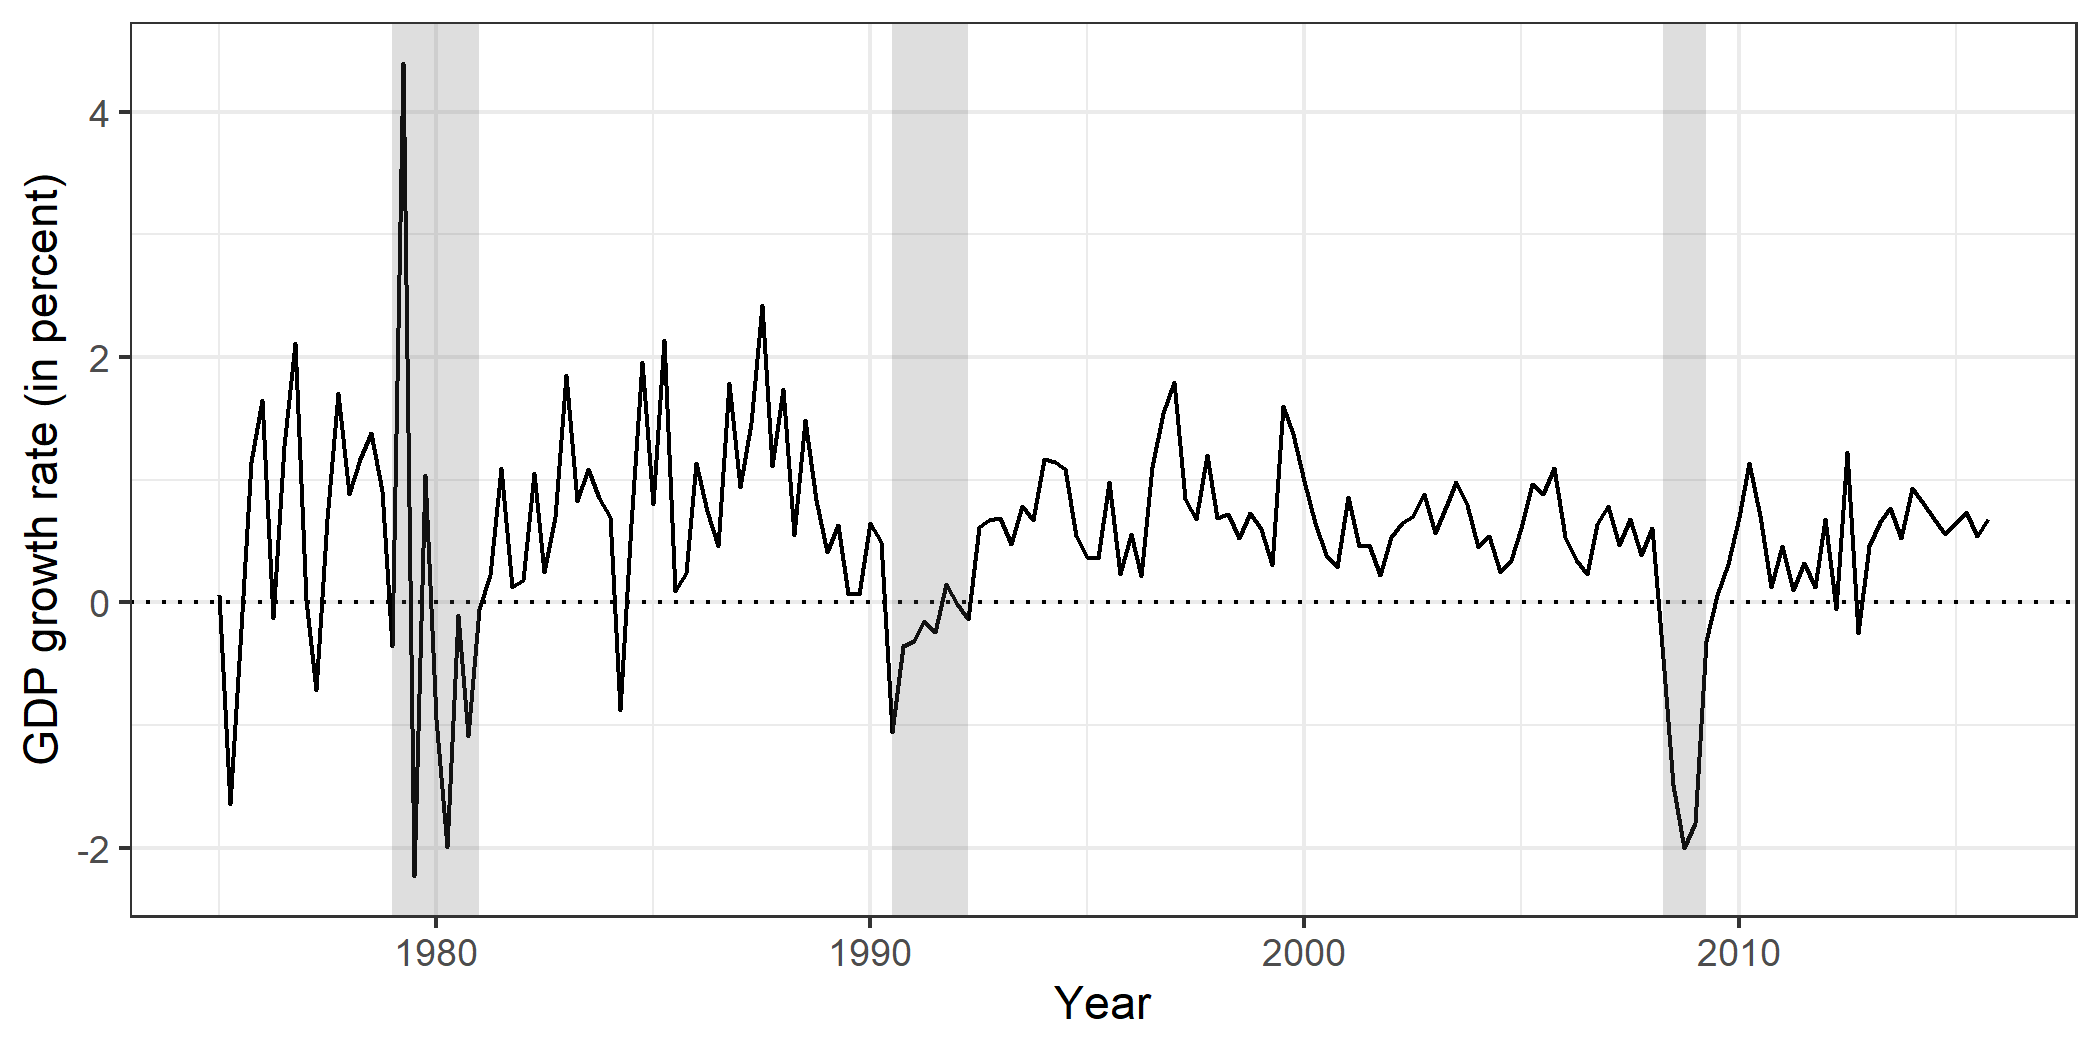
\includegraphics[width=\linewidth]{chap2/graphic/gdp-growth.png}
    \vspace{-3em}
	\justify\singlespacing\footnotesize{\textit{Notes:} This figure presents the quarterly GDP growth rate in the UK from 1975 to 2015. GDP is measured in chained volume and seasonally adjusted. Data are from the Office for National Statistics \href{https://www.ons.gov.uk/economy/grossdomesticproductgdp/timeseries/abmi/pn2}{Office for National Statistics}. Highlighted periods refer to recession periods in the UK.}
\end{figure}

Figure \ref{chap2-fig:lfs-national-cycle} presents the occupational dynamics for individuals born in the same years as our two cohorts using data from the LFS. Our estimates of probabilities for first-period and second-period occupations are performed at the start and the end of those curves. For the NCDS58, we consider their first period at age 23, hence in year 1981, which lies in a the Early 1980s recession. For other periods, they do not seem to be affected by business cycle dynamics as they follow the expected steady trends.
\begin{figure}[!htb]
    \centering
    \caption{LFS occupational dynamics over both cohort lifecycle}
    \label{chap2-fig:lfs-national-cycle}
    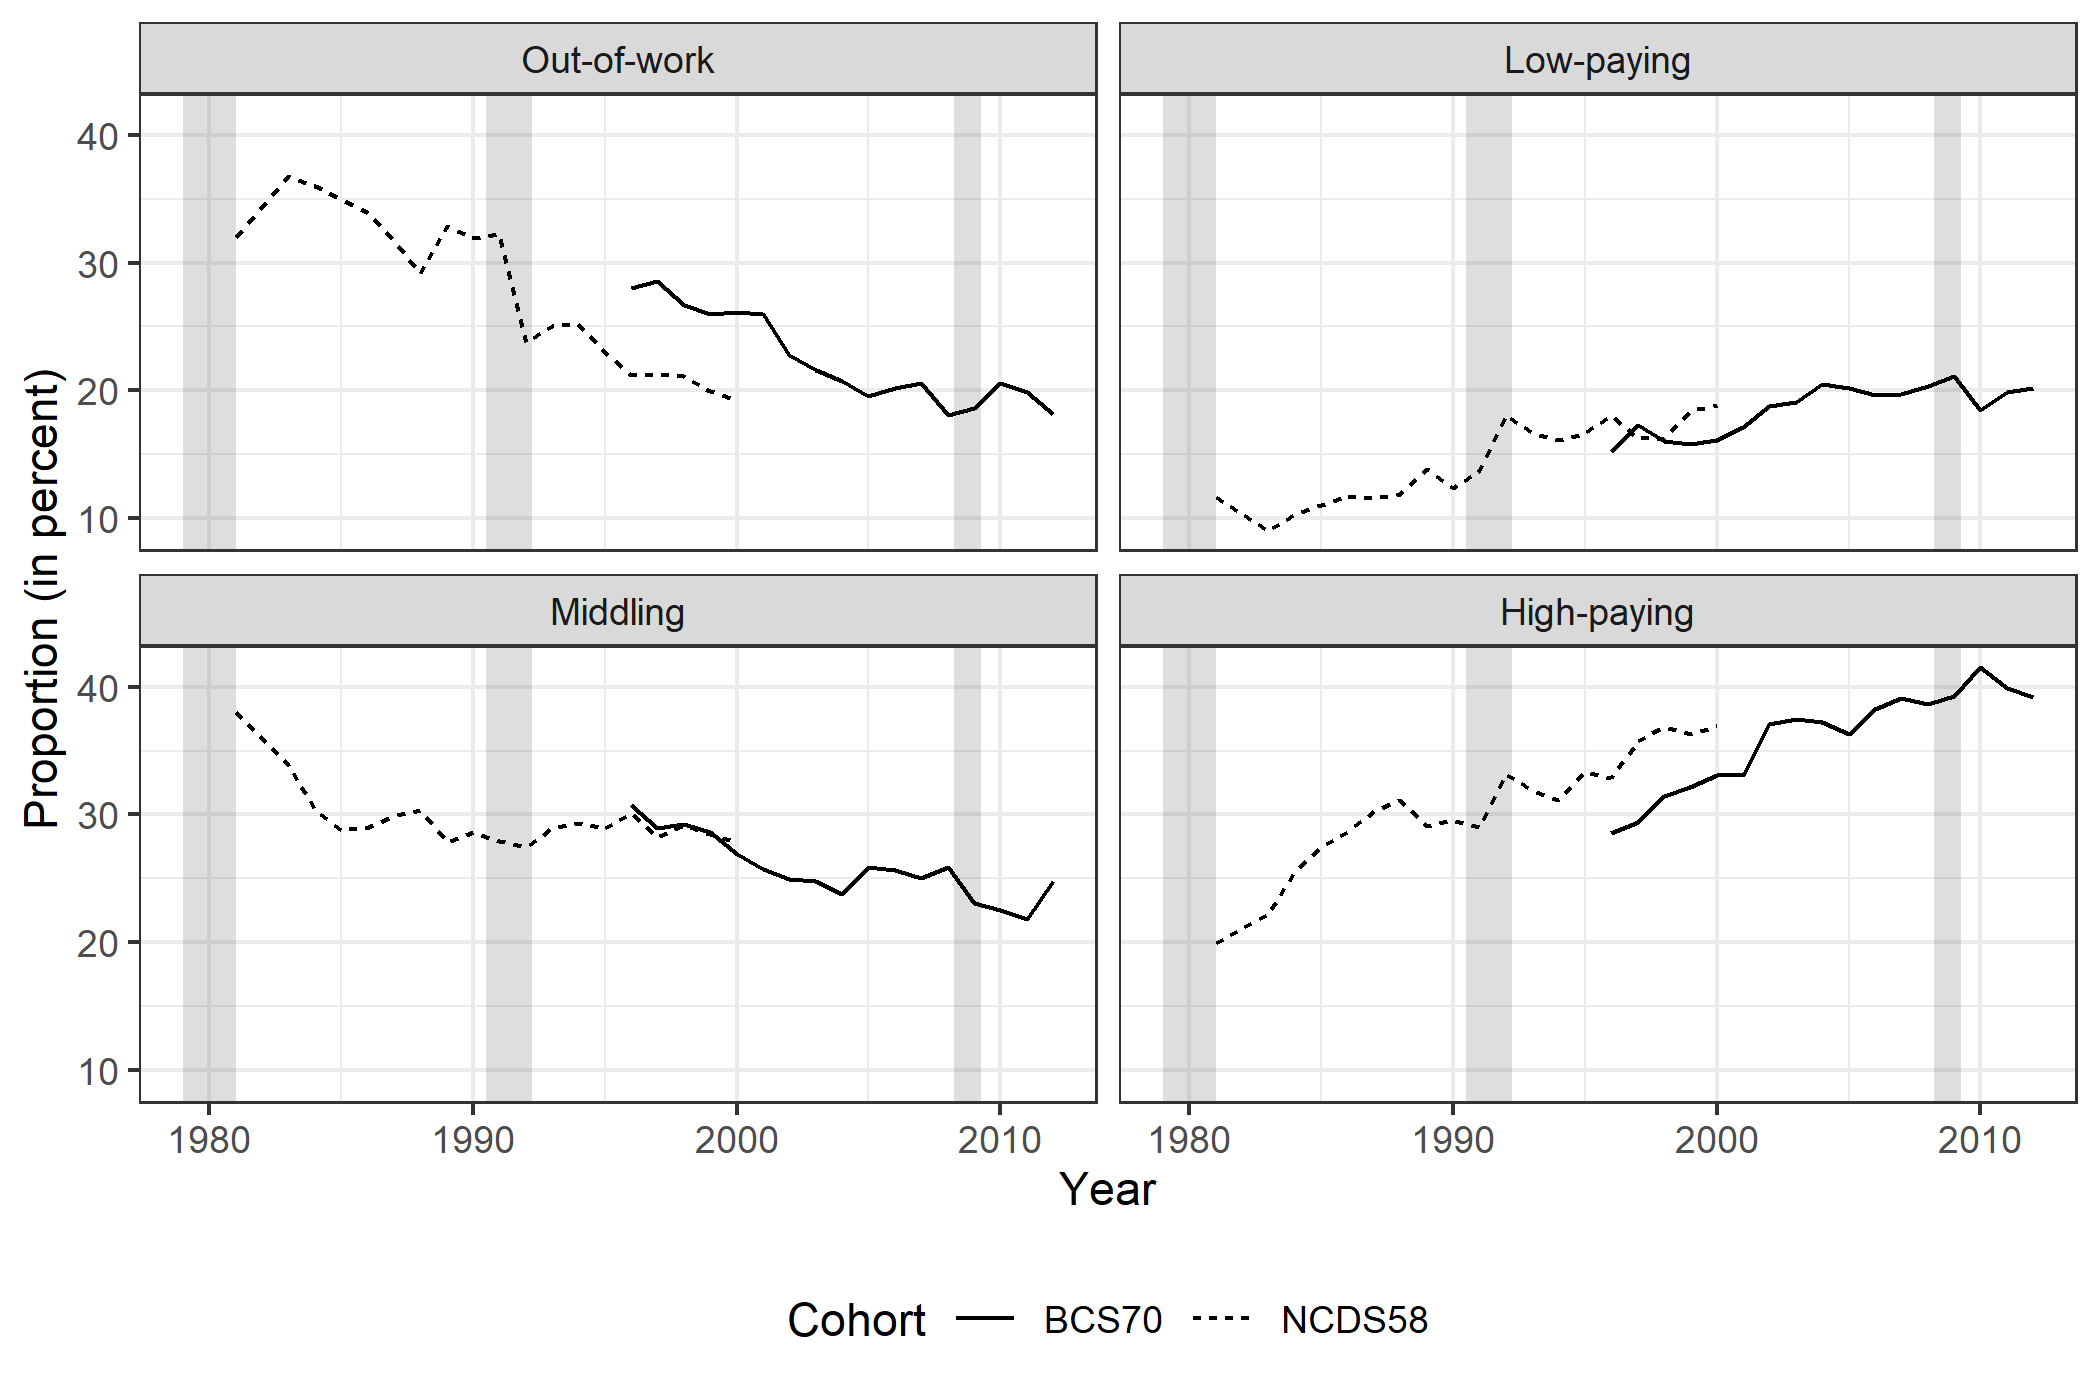
\includegraphics[width=\linewidth]{chap2/graphic/lfs-national-cycle.png}
    \vspace{-3em}
	\justify\singlespacing\footnotesize{\textit{Notes:} This figure presents the job polarization at the national level using the Labour Force Survey (LFS) data from 1981 to 2012. Curves represent the share of individuals in out-of-work, low-paying, middling, and high-paying occupations from the LFS for individuals born in the same year as the BCS70 and NCDS58 cohorts. Highlighted periods refer to recession periods in the UK.}
\end{figure}
The concern about the age of 23 as first period for the NCDS58 cohort can be addressed by looking at tables \ref{chap2-tab:rob2-multi1-base} and \ref{chap2-tab:rob2-multi3-base}. In those tables, we provide estimates of our main regressions when both cohorts are either 23 or 26 years old and show that our results are not driven by first-period age difference. The older cohort is age 26 in 1984 which does not lie in the Early 1980s recession.

\end{refsection}

	\chapter{Spillover effects across values}\label{chap3}
	\noindent \textbf{Abstract}: Values characterize preferences that themselves shape individuals’ decisions explaining future gaps in economic outcomes. I study the dynamics of values when values are inter-dependent and shocked by life events and I show that spillover effects across values do exist. Individuals choose to identify with a group with which they share values, but there are psychological costs to have values that are not consistent with those of the group. Whenever an event occurs in someone’s life---bringing new information---this may change some of her values. This shock can drive the individual to identify with a new group if the shocked values have taken her too far from her previous group. By identifying with the new group, she changes all her values---including not initially affected values---toward those of that new group. By changing values that are not affected by the shock, life events generate spillover effects across values.\\
\vspace{1em}\\
\noindent\textbf{Keywords:} Values dynamics; Cognitive dissonance; Spillover effects; Simultaneous equations model.\\
\noindent\textbf{JEL Codes:} A13, D63, D91, Z10.

\clearpage
\chaptertoc{}

\pagebreak

\begin{refsection}
    
    \section{Introduction} \label{chap3-introduction}
    Values are personal beliefs about what is important in individuals' lives and therefore characterize preferences.\footnote{Values differ from personality traits. Personality traits describe how individuals behave across time and situations, while values refer to what they consider important. See \citet{Schwartz2012Overview} for a discussion on how values relate to attitudes, beliefs, traits, and norms.}
For instance, universalism is a value which all of us hold to a certain extent; this, in turn, influences our preferences for redistribution (\citealt{Enke2020Moral}).
One can think of as many values as there are preferences (e.g. for leisure or for fertility).
Studying the dynamics of values is therefore crucial to understand differences in preferences between economic agents which explain differences in behaviors (e.g. effort or fertility decisions), hence, gaps in economic outcomes (e.g. wage or employment).
Although the inter-generational transmission is key in explaining the formation of values, their subsequent dynamics are driven by life experiences.

As the saying goes: ``a wise man changes his mind, a fool never will''. What the saying does not explain is why the wise man began to reassess his mind. One potential answer would be that something happened to him, but if that something also happened to the fool, such an answer is not sufficient. 
Another avenue is to ask whether they pay the same costs to change their minds or not. In the latter case, the fool would not be so much of a fool. Although he is a fool, he may have friends with whom he shares values, hence changing his mind is costly as it creates a distance between him and them. One may argue that the wise man bears the same cost as he also has friends who share values with him. 
The key point of that riddle is that the two groups of friends are drastically different in the values they convey, thus, values are inter-dependent within groups and both---the fool and the wise man---aim to be consistent with respect to values held in their groups. Therefore, the life-changing event may have changed one of the wise man's values which made him less compatible with his friends' values, hence, he preferred to identify with a new group of friends and therefore changed all his values toward those of that new group.

This paper argues that because group identity is defined by a cluster of values, shocks to one value that induce a change in group membership will lead to changes in other values, hence creating \textit{spillover effects}. Individuals are social and form groups based on values they share with others. Whenever an event occurs in someone's life, this brings new information and can generate a shock on some of her values. This shock can drive the individual to identify with a new group---because the shocked values have become too distant from those of her previous group. By identifying with the new group, she changes all her values---including not initially affected values---toward those of the new group. By changing values that are not affected by the shock, life events generate spillover effects across values.

Based on social psychology, I develop a model where the dynamics of values is disciplined by two anchoring forces: \textit{time consistency} and \textit{group consistency}. 
The former indicates that one prefers her today's values being close to her yesterday's values, that is, that values be consistent over time. This induces rigidity shaping how values adjust over time after a life-changing event that brings new information. 
The latter relates to the proximity of values held within the group with which we identify, hence, one prefers values to be consistent with those of her group. 
Both consistencies are based on the concept of cognitive dissonance introduced by \citet{Festinger1957Theory} as individuals seek to avoid the psychological burden of having values that are dissonant with either their past self or their group.

Following a life-changing event, the agent faces a consistency trade-off between time consistency and group consistency. An event corresponds to an information shock on one of her values at the end of a period. 
In the next period, the individual has to reset her values subject to both time and group consistencies. 
One way to soften such a trade-off consists of diminishing the dissonance with her group by identifying with a new group (e.g. new friends or a new political party) which conveys values that are closer to her recently shocked value.
Thus, with endogenous group membership, the agent will consider identifying with another group, which may imply resetting all her values toward the ones of this new group. 
For this to occur, the information shock needs to be sufficiently large to make this costly convergence process more desirable than keeping the previous group identity.

When values are independent, the agent adjusts her shocked value \textit{independently} of other values by simply minimizing the distance between her past value (time consistency) and the value of the group to which she decides to belong (group consistency).
The inter-dependence between values distorts the consistency trade-off.
When values are correlated within groups, the agent adjusts all her values \textit{simultaneously} as the relative weight of both consistencies depends on the intensity of the inter-dependence between values.\footnote{The intensity of the inter-dependence between values is exogenous to the agent and reflects the mapping of values in the society; see \citet{Roccas2010Personal} for the importance of the cultural context.}
Thus, the trade-off is in favor of the group consistency as the dissonance with the current group occurs across several dimensions.
As a result, the information shock on one value that would lead the agent to identify with another group has to be larger than the one that is needed when values are independent. 
Yet, if such a shock occurs on a value, then the agent identifies with a new group and changes all her values toward the ones of the new group, hence, triggering the so-called \textit{spillover effect}.

I test the prediction of the theory about the existence of spillover effects by using data from two British cohort studies in which I measure individuals' values and observe political vote at several ages. Using a principal component analysis, I show that the variation in the answers to a large set of questions about values can be summarized by two main dimensions which will be the two values of my latter analysis. These two dimensions coincide with the (motivational types of) values introduced by \citet{Schwartz1992Universals, Schwartz2012Overview}.
% CONSERVATION VS OPENNESS TO CHANGE
The first dimension captures conservation versus openness to change---the preference for stability, security, tradition, and conformity versus the openness to new experiences related to self-direction and stimulation. For ease of exposition, in what follows, I refer to those values as \textit{conservatism} versus \textit{progressivism}.
% SELF TRANSCENDENCE VERSUS SELF ENHANCEMENT
The second dimension reflects self-transcendence versus self-enhancement---values associated to care for and concern about others such as universalism and benevolence versus the self-interest and ambition linked to achievement and power. In what follows, I refer to them as \textit{collectivism} versus \textit{individualism}.

%% Political vote
I use the political vote of individuals at the general election to proxy their group membership. The mapping of voters is consistent with the two-dimensional value space across cohorts and periods. For instance, Conservative voters tend to have conservative and individualist values, whereas Labour voters are instead progressive and collectivist.

%% OLS
The identification of changes in values and group membership is challenging. 
I start by estimating separately the effect of two exogenous and non-reversible life events---to have a girl as a first child (conditional on having a baby), and to have ever had cancer---on both individuals' values. Individuals who went through one of those two life events tend to have more conservative values but there are no significant differences in collectivism. 
Then, I estimate the probability to vote for each political party at the general election according to changes in values since the previous period. Changes in values are associated with changes in the likelihood to vote for the political parties, hence, with changes in the probability to identify with a new group.

%% IV
To examine the presence of spillover effects, I instrument conservatism by the information shock associated to the life event and then I look at the impact on collectivism. A one-standard-deviation increase in conservatism induces an increase in individualism of about one third of a standard deviation. Using the first-stage regression to estimate the probability of voting for each political party also indicates that increasing conservatism promotes the probability of voting for right-wing political parties over left-wing ones. Thus, providing empirical evidence of the group membership as the underlying mechanism in explaining the existence of spillover effects.

% SEM
The identification relies on the assumption that each life event brings no information shock on collective values. The identification assumption may be violated for many life events. For instance, to have ever been unemployed is likely to bring information shocks on both values, hence, the spillover effects cannot be identified in that setting. To deal with the two-side effect of unemployment on values that threatens identification, I use a simultaneous equations model in which I instrument endogenous values with their own respective lags.\footnote{I also address the question of the endogeneity of the life-event with respect to values in the case of unemployment. From the theoretical framework, I derive an expression of this bias that is a scale multiplier of the direct and indirect effects, hence, of the total effect. I show that \textit{i)} the bias can affect the magnitude of the total effect without changing the qualitative result, \textit{ii)} it is still possible to provide a lower-bound estimate of the effect, and \textit{iii)} the bias does not change the relative share of the total effect that is due to the direct and the spillover effects.} Thus, the identification relies on symmetrical exclusion restrictions which assume that one value is not directly affected by the lag of the other value. Based on the simultaneous equations model, I can estimate and decompose the change in values due to the information shock (direct effect) and the change owing to spillover effects across values (indirect effect). 

% RESULT 1
My empirical analysis yields three main results. First, life events change values throughout the lifecycle. Both exogenous life-changing events---to have a girl as a first child and to have ever had cancer---increase conservative values, while to have never been unemployed make individuals more progressive. Collectivist values are fostered by both the latter event and having ever had cancer.

% RESULT 2
Second, changes in values are associated with changes in political voting, hence, group membership. On the one hand, when individuals become more conservative they also become more likely to vote for right-wing political parties (e.g. Conservative Party or UKIP) with respect to left-wing ones (e.g. Labour Party or Green Party). On the other hand, when individuals become more collectivist they shift their vote toward non-traditional political parties (e.g. Green Party, or UKIP) instead of traditional ones (i.e. Conservative Party and Labor Party).

% RESULT 3
Third, life events affect both values at the same time since spillover effects across values do exist. After an increase in conservatism due to a life-changing event, collectivism declines by a third of the increase in conservatism. Once the framework is generalized to shocks that can simultaneously affect both values, the spillover effects become non-reciprocal: an increase in conservatism still generates a \textit{negative} spillover effect on collectivism; but an increase in collectivism generates a \textit{positive} spillover effect on conservatism. Thus, there is a spiral pattern in the dynamics between values that can be rationalized by the dynamic underpinnings of value changes from the social psychology literature (\citealt{Schwartz2012Overview}).

% CONTRIB 1
This paper is the first to show the existence of spillover effects across values by considering the multi-dimensionality of values that characterizes group identity as a cluster of values. Prior work analyses the dynamics of values but focuses on the evolution of a single value (\citealt{Piketty1995Social}, \citealt{Mayda2006Against}, \citealt{Fernandez2007Women}, \citealt{Alesina2018Intergenerational}, i.a.). I contribute to this literature by showing that neglecting the inter-dependence between values---i.e. assuming that values are independent---underestimates to which extent life experiences affect individuals because this omits the consequences of the group membership, hence, the spillover effects.

This paper adds to the literature on the formation and dynamics of values. Prior work highlights several mechanisms such as the inter-generational transmission (\citealt{Bisin2001Economics, Bisin2011Economics}, \citealt{Montgomery2010Intergenerational}, \citealt{Hiller2016Cultural}, \citealt{Alan2017Transmission}, i.a.) along with the role of cultural values (\citealt{Ichino2000Work}, \citealt{Fernandez2004Mothers}, \citealt{Guiso2006Culture}, \citealt{Fernandez2007Women}, \citealt{Giuliano2007Living}, \citealt{Chen2013Effect}, \citealt{Alesina2014Family}) and norms (\citealt{Fehr2002Psychological}, \citealt{Bardi2003Values}, \citealt{Tabellini2008Scope}) to explain how people form their values. Recent work focuses on the development of values during childhood (\citealt{Fehr2013Development}, \citealt{Doepke2017Parenting}, \citealt{Basic2020Development}).
I contribute to this literature by providing an additional mechanism based on cognitive dissonance and endogenous group membership (i.e. identity).

My work is also related to the literature on the consequences of cognitive dissonance in economics (\citealt{Akerlof1982Cognitive}, \citealt{Konow2000Fair}, \citealt{Benabou2006Belief}).
Prior work uses the concept of cognitive dissonance---introduced by \citet{Festinger1957Theory} and \citet{McGuire1960Cognitive}---to explain the belief-behavior relationship. I, instead, consider its effects on the between-values relationship; either to avoid dissonance with the previous self (\citealt{Eyster2002Rationalizing}, \citealt{Yariv2002See}) or to avoid dissonance with the values of the group.

My approach is also inspired by the literature on identity in economics (\citealt{Akerlof2005Identity, Akerlof2010Identity}, \citealt{Benabou2011Identity}, \citealt{Kranton2016Identity}). Prior work shows the effect of group membership on individual behavior (\citealt{Charness2007Individual}, \citealt{Sutter2009Individual}). I link changes in values, hence spillover effects, to change in endogenous group membership. Thus, individuals decide with which group they prefer to identify by comparing their values with the ones held in these groups.
In the empirical part, I build my identification strategy of changes in group membership using political identity (\citealt{Shayo2009Model}, \citealt{Bonomi2021Identity}).

My work also builds an additional bridge between the social psychology literature and that in economics. Psychological determinants of economic behaviors have been mostly introduced through personality traits (\citealt{Borghans2008Economics}, \citealt{Almlund2011Personality}, \citealt{Ferguson2011Personality}, \citealt{Becker2012Relationship}, \citealt{Flinn2018Personality}, \citealt{Todd2020Dynamic}). 
The \textit{big-five} personality traits are quite stable over the lifecycle and therefore can hardly explain changes in individuals' decision-making process (\citealt{Terracciano2006Personality, Terracciano2010Intra}, \citealt{Cobb-Clark2012Stability}). Thus, I introduce motivational types of values \textit{à la} \citet{Schwartz1992Universals, Schwartz2012Overview} as novel determinants of economic behaviors, which are more volatile than personality traits because of the impact of life experiences (\citealt{Lonnqvist2011Personal}, \citealt{Daniel2021Changes}).
Yet, personality traits and values are related as they look at the same object, individuals, from different perspectives which are therefore complementary (\citealt{Caprara2009Mediational}, \citealt{Fischer2015Motivational}, \citealt{Parks2015Personality}).

Lastly, my results on the consequences of life-changing events relate to three additional literatures. First, to the literature on the impact of children's gender on their parents' views.
\citet{Washington2008Female} finds that congressmen become more progressive in their voting after having a daughter. I, instead, find that having a girl as a first child makes parents more conservative. I show that both results can be reconciled as I find that tertiary-educated parents become indeed more progressive after having a girl. This suggests that \citet{Washington2008Female} captures the effect of having a daughter at the top of the distribution since congressmen tend to be highly educated; whereas I capture the average effect.
\citet{Grinza2017Entry} argue that, when entering into parenthood, women shift toward more conservative views.\footnote{Similarly, \citet{Bolzendahl2004Feminist} and \citet{Cunningham2005Reciprocal} find that entry into parenthood reduces the support for egalitarian roles for women and men in families.}
I provide additional evidence to this literature by showing that the effect is all the more important when they have a daughter and that changes in values are larger for mothers than for fathers.

Second, my work also relates to the literature on the impact of cancer on employment.
\citet{Peteet2000Cancer} discusses the relationship between cancer and the meaning of work, in a context where the loss of occupational identity becomes a source of anxiety and depression. \citet{Moran2011Long} show that cancer survivors have lower employment rates and work fewer hours than other similarly aged adults which can be due to consequences on life purpose and limitations in the ability to work (\citealt{Short2005Employment, Short2008Work, Short2008Long}, \citealt{Bradley2002Breast, Bradley2005Short}, i.a.). I add to this literature by providing an underlying mechanism through which cancer has consequences for employment, hence, through changes in values.

Third, my results relate to the literature on unemployment scarring as they open another potential explanation for this phenomenon. Unemployment is known to have consequences on well-being and health (\citealt{Clark1994Unhappiness}, \citealt{Knabe2010Dissatisfied}, \citealt{Nordt2015Modelling}). Scarring emphasizes the depreciation of human capital and firm-specific skills as the main driver of future employment (\citealt{Arulampalam2001Unemployment}, \citealt{Clark2001Scarring}, \citealt{Gregg2005Wage}). I show that having ever been unemployed decreases individualism, thus, if the likelihood to find a job is an increasing function of individualist values, then my framework would provide a novel mechanism in which past unemployment could affect future employment through changes in values.

The remainder of the paper proceeds as follows. Section \ref{chap3-theoretical} presents the theoretical framework and emphasizes the role of inter-dependence between values and consistency. Section \ref{chap3-data} describes the cohort data, derives values, shows the mapping of political parties on the two-dimensional value space, and presents the life events that are used as information shocks in the empirical part. Section \ref{chap3-empirics} shows the presence of spillover effects using instrumental variable regressions. Section \ref{chap3-simultaneous} presents the simultaneous equations model to identify spillover effects when the information shock affects both values simultaneously, and then discusses the dynamics between values in light of the social psychology literature. Section \ref{chap3-conclusion} concludes.

    
    \section{Theoretical framework} \label{chap3-theoretical}
    % EXPLAIN THE MODEL
In this section, I develop a model to illustrate the role of dependent values when looking at the trade-off between time consistency and group consistency. I proceed in two steps. First, I describe the baseline model with only one value and show the consequences of an information shock. Then, I replicate the process in a model with two values that are correlated across groups. Thus, I discuss the difference with respect to the single-value model. Lastly, I state the predictions of the model.

\subsection{Single-value model}

Consider an agent with one value $a_t \in \mathbb{R}^2$.\footnote{The agent considers her value with respect to the norm, namely, the average value within the reference population. The reference population can be defined at several levels such as the city, the region, the country, or more broadly, the shared culture. See \citet{Roccas2010Personal} for the importance of the cultural context in the value-behavior relation. See, also, \citet{Bisin2011Economics} for a survey on the economics of cultural transmission and \citet{Rapport2014Social} for a survey on cultural heterogeneity in cultural anthropology. Hence, values are normalized to the population level, so that the mean value in the population is equal to zero.}
The agent belongs to group $s \in \{\underline{s}, \overline{s}\}$ which gather other agents with similar values together.\footnote{They can be seen as close people (including relatives, neighbors, colleagues) since individuals' values are on average correlated within these relationships. But, in a more general setup, they can be seen as peers with whom the agent wants to identify in terms of values.}
The average values within both groups are respectively $\underline{a}$ and $\overline{a}$. 
Suppose the population is sufficiently large to ensure \textit{anonymity}, meaning that any change of value from the agent does not change the distribution, hence, the average values within both groups.
For the remaining of the paper, I set $\overline{a} > 0 > \underline{a}$.

In any period $t$, the agent solves the following maximization program in order to determine her values and the group to which she belongs:
\begin{equation}
    \max_{a_t, s_t} U_t(a_t, s_t) = -\eta_a\frac{\left[a_t-a_{t-1}\right]^2}{2} -\phi_a\frac{\left[a_t-a^\star(s_t)\right]^2}{2},\label{chap3-eq:maxU-1val}
\end{equation}
where $a^\star(s_t)=\{\underline{a}, \overline{a}\}$ is the average value $a$ within her group and $(\eta_a, \phi_a) \in (\mathbb{R}_{+}^\star)^2$ are parameters that account for the relative importance of each utility components.\footnote{These parameters are assumed to be homogeneous within the population, although they might differ across groups of individuals. More extensively, the emergence of heterogeneity in the relative importance of each component would be an interesting point that I leave for future research.} Components of the utility function are expressed in one-dimension Euclidean squared distances. 

The agent seeks to avoid two psychological costs, namely, \textit{time inconsistency} and \textit{group dissonance}. The former implies that the agent prefers when her today’s values are close from her yesterday’s values, thus, she suffers from a utility loss the further her value in period $t$ is from her value in period $t-1$, i.e. $a_t - a_{t-1}$. The literature on social psychology shows that individuals tend to resist changing their attitudes, beliefs, and values through behaviors such as cognitive inertia, or belief perseverance, providing empirical evidence of such a component in agent's utility; see \citet{Kunda1990Case} for a review of biased information processing through which people maintain their beliefs.

The latter psychological cost implies that the agent prefers to hold values that are close to norms within the group to whom she belongs, hence, having a disutility the further her value is from the average value within her group, i.e. $a_t-a^\star(s_t)$. The consistency with the group---to avoid group dissonance---refers to the concept of conformity warp in the social economics literature, meaning that individuals are warped away from their optimal behavior, here values, because they have to conform to the norm; see \citet{Burke2011Social} for a survey on the role of social norms and individual behaviors in presence of norms.

%%%%% OPTIMAL VALUES %%%%%
The optimal value satisfies both the time and group consistencies, hence, it is equal to the weighted average between the agent's value in previous period and the average value in her group. It corresponds to the first-order condition that solves the maximization program \eqref{chap3-eq:maxU-1val}, namely,
\begin{equation}\label{chap3-eq:foc-1val}
    a_t(s_t) =  \frac{\eta_a a_{t-1} + \phi_a a^\star(s_t)}{\eta_a + \phi_a}.
\end{equation}
Thus, the optimal value depends on the group to which the agent decides to belong, hence, to identify.

Suppose that group membership is exogenous, meaning that the agent cannot identify with another group. Thus, she has an initial value $a_0$ and belongs to a group with $a^\star$ as the group-average value. 
The dynamics of the value $a_t$ is derived from equation \eqref{chap3-eq:foc-1val} and correspond to
\begin{equation}\label{chap3-eq:dyn-1val}
    a_t = a^\star + \left(\frac{\eta_a}{\eta_a+\phi_a}\right)^t(a_0-a^\star).
\end{equation}
It is straightforward to show that the value converges toward the average of the group, i.e. $\lim_{t\to+\infty} a_t = a^\star$, at a rate of convergence
\begin{equation*}
    \lim_{t\to+\infty} \frac{\left|a_{t+1}-a^\star\right|}{\left|a_{t}-a^\star\right|} = \frac{\eta_a}{\eta_a+\phi_a} < 1.
\end{equation*}
Thus, leading to Proposition \ref{chap3-prp:converge}. Proof in appendix \ref{chap3-model}.
\begin{proposition}[Value convergence]\label{chap3-prp:converge}
    Any individual converges to the average value within her group and the speed of convergence depends positively on the relative weight of the group consistency (with respect to the time consistency) in the utility function.
\end{proposition}

Let allow the agent to freely choose her group.\footnote{I do not consider any uncertainty in the ability to identify with a group neither any direct cost. Nonetheless, the group consistency corresponds to the psychological, hence indirect, cost of changing group.} She compares both indirect utilities to determine which group she prefers, i.e. $U_t(\overline{s}) - U_t(\underline{s})$. Using the utility function from the maximization problem \eqref{chap3-eq:maxU-1val} along with the optimal value in equation \eqref{chap3-eq:foc-1val}, I obtain
\begin{equation}\label{chap3-eq:uovers-uunders}
    U_t(\overline{s}) - U_t(\underline{s}) = -\gamma_a \left(\left[\overline{a}-a_{t-1}\right]^2 - \left[a_{t-1}-\underline{a}\right]^2\right),
\end{equation}
where $\gamma_a \equiv \frac{\eta_a\phi_a}{2(\eta_a+\phi_a)} >0$. The agent weakly prefers her group to the other as long as her indirect utility in this group is greater or equal to the one she would get in the other.

%%%%% VALUE CONVERGENCE IN SINGLE-VALUE MODEL %%%%%
Let $\widetilde{a}$ be the \textit{indifference value} which is defined as the threshold value in $t-1$ such that the agent is indifferent between both groups in period $t$, i.e. $U_t(\overline{s}) - U_t(\underline{s}) = 0$.
Using equation \eqref{chap3-eq:uovers-uunders}, the indifference value is $\widetilde{a} = \widehat{a}$, where $\widehat{a} \equiv (\overline{a}+\underline{a})/2$ is the \textit{midpoint value}.
The midpoint value refers to the middle of the distance between the average values in both groups and represents the frontier between both groups.\footnote{The anonymity of the agent ensures that the frontier is exogenous.}

Figure \ref{chap3-fig:theory-choice-a} illustrates the indifference value and group membership.
\begin{figure}[!tb]
    \centering
    \caption{Indifference value and group membership}
    \label{chap3-fig:theory-choice-a}
    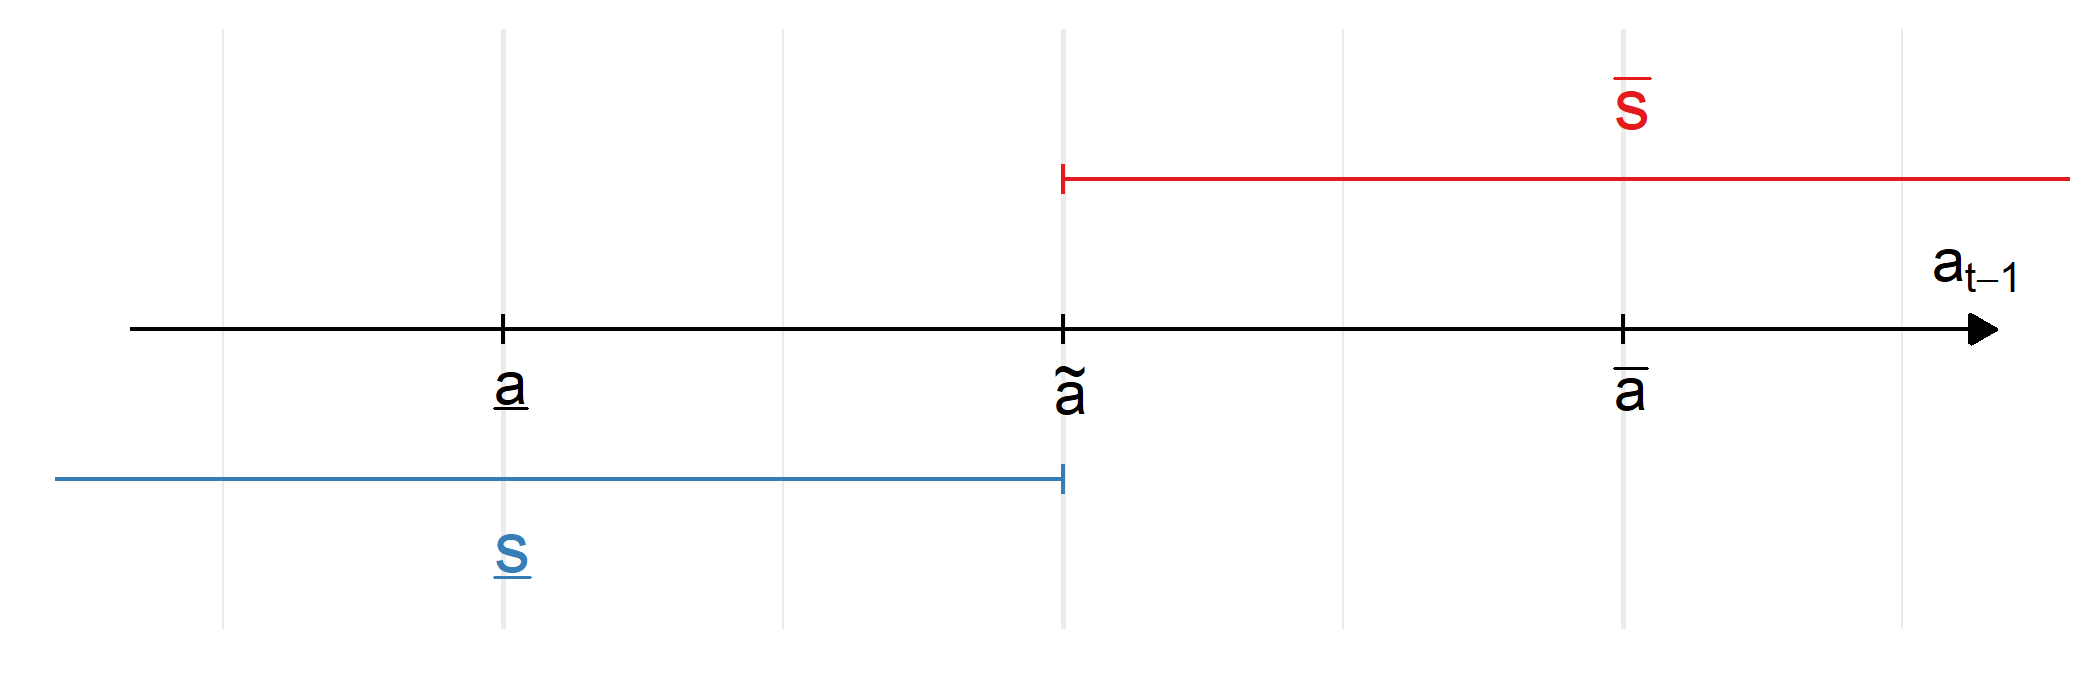
\includegraphics[width=.8\linewidth]{chap3/graphic/theory-choice-a.png}
	\vspace{-3em}
	\justify\singlespacing\footnotesize{\textit{Notes:} This figure presents the indifference value $\widetilde{a}_{t-1}$ which is defined as the threshold value $a$ in $t-1$ such that the agent is indifferent between both groups. In the single-value model, it corresponds to the midpoint value $\widehat{a}$, which is the middle of the distance between the average values in both groups. When the value $a$ in previous period is lower (resp. higher) than the indifference value, the agent prefers to identify with the group $\underline{s}$ (resp. $\overline{s}$).}
\end{figure}
In the single-value model, as long as the value in previous period $a_{t-1}$ is greater (resp. smaller) than the midpoint value $\widehat{a}$, the agent prefers to belong to group $\overline{s}$ (resp. $\underline{s}$). In absence of shocks on her value, the agent converges toward a steady-state value which corresponds to the average value within her group, and the dynamics is given by equation \eqref{chap3-eq:dyn-1val}. What happens when there is a shock?


If an information shock is sufficiently large, the agent identifies with the other group.\footnote{Based on constructivist psychology, a shock on values consists of an event that brings new information to the agent through an experience (\citealt{Levitt2004Transformational}). This latter challenges the agent by questioning her sense of independence, her emotions, her self-awareness, hence, all her perceptions of the meaning of life (i.e. values).} Suppose the agent belongs to the group $\underline{s}$ and she is in her steady state which means that $a_{t-1} = \underline{a}$. There is a shock $\Delta a_{t-1}$ at the end of the period such that her value becomes $a_{t-1}^\prime = a_{t-1} + \Delta a_{t-1}$. Thus, it is straightforward that the agent prefers to keep with her current group $\underline{s}$ as long as the shock does not push $a_{t-1}^\prime$ beyond the threshold---characterized by the indifference value $\widetilde{a}$. Otherwise, the agent prefers to identify with the other group $\overline{s}$. This result leads to Proposition \ref{chap3-prp:shock}. Proof in appendix \ref{chap3-model}.
\begin{proposition}[Shock existence]\label{chap3-prp:shock}
    For any individual, it always exists an information shock such that she prefers to identify with the other group.
\end{proposition}

%%%%% RESULT 1 %%%%%
The single-value model delivers two main results. First, any individual converges to the average value within her group. The length of time to convergence depends on two components: the rate of convergence and the distance with the group-average value. 
On the one hand, the greater is the ratio $\eta_a/\phi_a$, the more costly is the time inconsistency with respect to the group dissonance, hence, the faster the convergence. 
On the other hand, the further the current value is from the group-average value, the slower the convergence.

%%%%% RESULT 2 %%%%%
Second, it is always possible to find a shock such that an individual starts to identify with the other group. The shock requires two conditions to be satisfied: its direction has to be toward the other-group average value and the magnitude has to be sufficiently large. The magnitude depends on the distance between both groups in terms of value and the current value of the individual. The larger is the distance, the greater has to be the shock. When the current value is in a steady state, the magnitude corresponds to the midpoint distance. Otherwise, the closer she is from the midpoint value, the smaller has to be the shock.

\subsection{Two-value model}

We aim to understand the difference in terms of values dynamics when there are two values instead of one. Suppose there are two (motivational types of) values $V_t = (a_t, b_t)\in\mathbb{R}^2$. Consider the same utility function as before but including the second value $b_t$. The maximization program of the agent becomes:
\begin{equation}\label{chap3-eq:maxU-2val}
    \begin{split}
        \max_{a_t, b_t, s_t} U_t(a_t, b_t, s_t) = &-\eta_a\frac{\left[a_t-a_{t-1}\right]^2}{2} -\phi_a\frac{\left[a_t-a^\star(s_t)\right]^2}{2}\\
        &-\eta_b\frac{\left[b_t-b_{t-1}\right]^2}{2} -\phi_b\frac{\left[b_t-b^\star(s_t)\right]^2}{2},
    \end{split}
\end{equation}
where $v^\star(s_t) = \{\underline{v}, \overline{v}\}$ is the average-group value $v\in\{a,b\}$ and $(\eta_a, \phi_a, \eta_b, \phi_b)\in (\mathbb{R}^\star_{+})^4$ are parameters that account for the relative importance of each utility components. 
%
The agent seeks to avoid the same psychological costs as before, namely, time inconsistency and group dissonance, but on two values instead of one. The optimal values are identical to the single-value model, hence, the weighted average between the past value and the average value within the group:
\begin{align*}
    a_t(s_t) =  \frac{\eta_a a_{t-1} + \phi_a a^\star(s_t)}{\eta_a + \phi_a}, \hspace{2em} \text{and} \hspace{2em}%\label{chap3-eq:foc-1val-a}
    b_t(s_t) =  \frac{\eta_b b_{t-1} + \phi_b b^\star(s_t)}{\eta_b + \phi_b}.%\label{chap3-eq:foc-1val-b}
\end{align*}
Thus, the dynamics of values are also identical to equation \eqref{chap3-eq:dyn-1val} and Proposition \ref{chap3-prp:converge} holds. So far, nothing changes with respect to the single-value model although we add one value.

The difference in this setup arises from the inter-dependence between both values. There exist two groups, $\underline{s}$ and $\overline{s}$, in which the average values are respectively $(\underline{a}, \underline{b})$ and $(\overline{a}, \overline{b})$.
Since values are standardized in the population, it implies that $\underline{v}$ and $\overline{v}$ have opposite signs. 
%
We have set the average value $a$ in both groups such that $\overline{a} > 0 > \underline{a}$.
%
Thus, the inter-dependence between values is captured by the sign of $\overline{b}$ (or equivalently by the sign of $\underline{b}$). If $\overline{b}$ is positive, then both values are positively correlated in the population. Otherwise, they are negatively correlated. 

The inter-dependence between values affects the conditions under which the agent prefers to change her group. To illustrate this, suppose the agent belongs to the group $\underline{s}$ and she is in her steady state such that $a_{t-1}=\underline{a}$ and $b_{t-1} = \underline{b}$.
%
There is an information shock on value $a$ at the end of the period, hence, $a_{t-1}^\prime = \underline{a} + \Delta a_{t-1}$. In period $t$, the agent has to choose whether she wants to stay in her group or change for the other group. Her values depend on this choice. If she decides to stay in her current group, her indirect utility is
\begin{equation}\label{chap3-eq:U1under}
    U_t(\underline{s}) = - \gamma_a \left(\Delta a_{t-1}\right)^2.
\end{equation}
Otherwise, she changes her group and gets the following indirect utility:
\begin{equation}\label{chap3-eq:U1over}
    U_t(\overline{s}) = - \gamma_a \big[\overline{a} - \underline{a}-\Delta a_{t-1}\big]^2
    - \gamma_b \big[\overline{b}-\underline{b}\big]^2,
\end{equation}
where $\gamma_b \equiv \frac{\eta_b\phi_b}{2(\eta_b+\phi_b)}>0$. 

The agent decides to change her group \textit{if and only if} the information shock drives her value $a^\prime_{t-1}$ beyond the indifference threshold $\widetilde{a}$, as depicted in figure \ref{chap3-fig:theory-choice-a}. In this example, the indifference value is derived from equations \eqref{chap3-eq:U1under} and \eqref{chap3-eq:U1over} and corresponds to
\begin{equation}\label{chap3-eq:indiff}
    \widetilde{a} = \widehat{a} + \frac{1}{2\gamma}\frac{\big(\overline{b}-\underline{b}\big)^2}{\overline{a}-\underline{a}},
\end{equation}
where $\gamma \equiv \gamma_a/\gamma_b > 0$ and $\overline{a}-\underline{a} > 0$ by definition.
When both values are orthogonal, i.e. $\overline{b}-\underline{b} = 0$, the indifference value corresponds to the one of the single-value model, namely, $\widehat{a}$.

Figure \ref{chap3-fig:theory-shift-a} presents the indifference value as a function of the degree of inter-dependence between values.
\begin{figure}[!tb]
    \centering
    \caption{Indifference value and inter-dependence between values}
    \label{chap3-fig:theory-shift-a}
    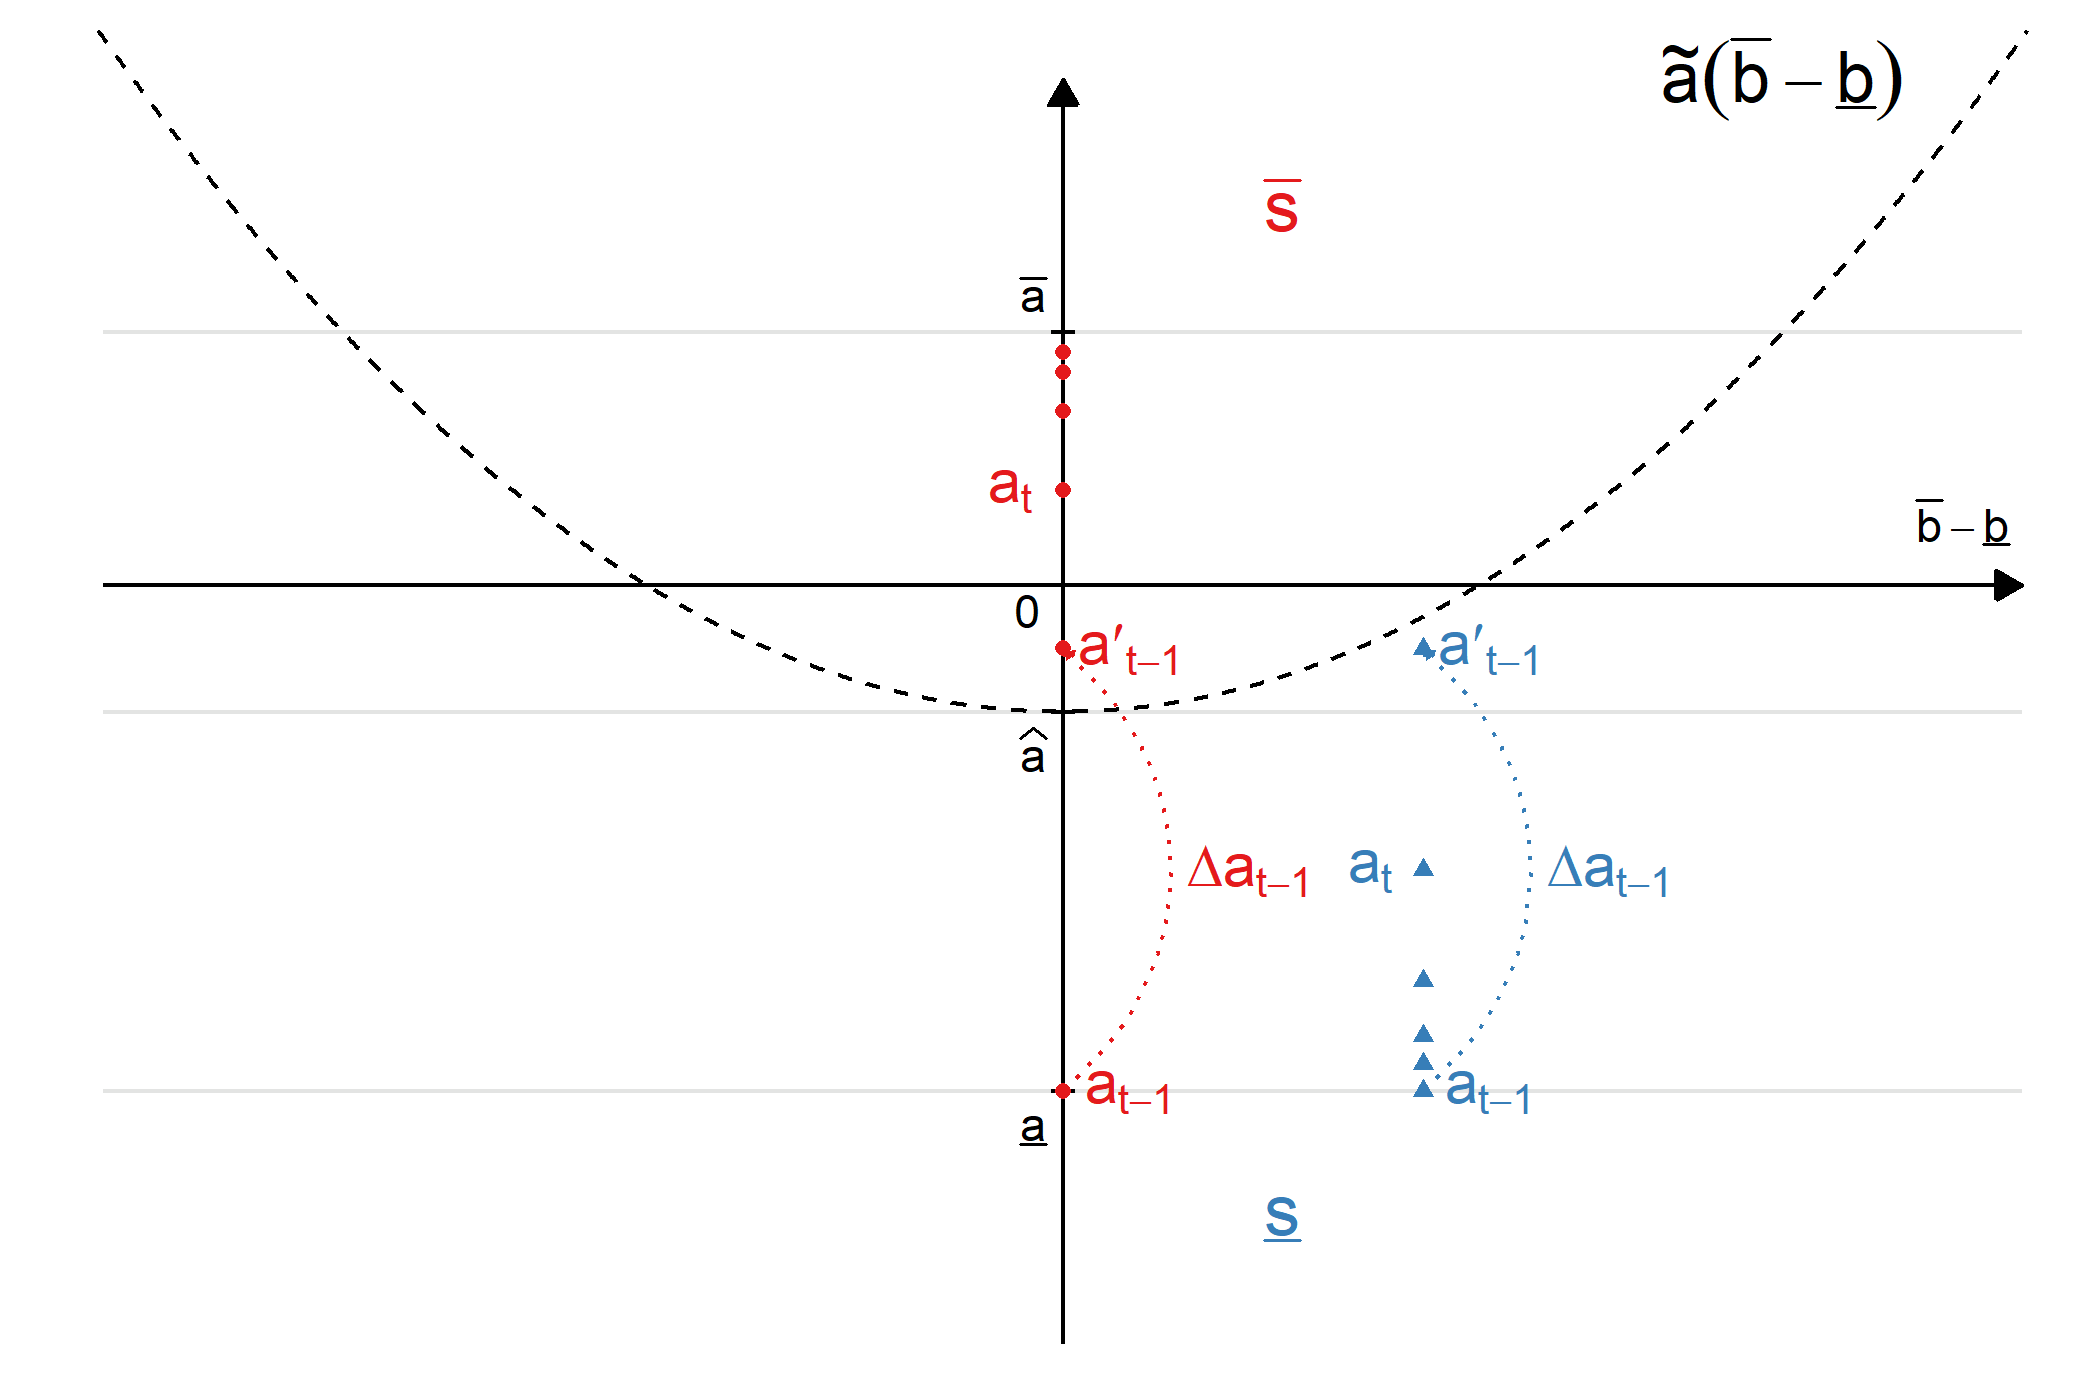
\includegraphics[width=\linewidth]{chap3/graphic/theory-shift-a.png}
	\vspace{-3em}
	\justify\singlespacing\footnotesize{\textit{Notes:} This figure presents the indifference value as a function of the degree of inter-dependence between values. The x-axis corresponds to the gap between both group averages in terms of value $b$. As $\overline{a}-\underline{a} > 0$, it implies that the magnitude of $\overline{b}-\underline{b}$ corresponds to the degree of inter-dependence---values are either positively correlated on the right-hand side of the figure or negatively correlated on the left-hand side.
	The y-axis corresponds to the value $a$. 
	The dash line refers to the indifference value $\widetilde{a}$ and indicates the frontier of indifference between both groups $\overline{s}$ and $\underline{s}$. The dotted curve shows an information shock $\Delta a_{t-1}$ in two different settings, based on the degree of inter-dependence, which lead to different group memberships.}
\end{figure}
The right-hand side of the figure corresponds to cases in which both values are positively correlated, whereas the left-hand side refers to those in which they are negatively correlated. The dashed line represents the indifference value $\widetilde{a}$, which is a function of the distance between both group-average values in $b$, hence, the inter-dependency.

Starting with the area below the dashed curve, any information shock that shifts the value $a$ in this area is not sufficiently large to change the agent's group membership. Thus, agent's value $a$ converges back to its steady-state value $\underline{a}$, and value $b$ has not changed meanwhile.
Conversely, any information shock that brings the value $a$ above the indifference value implies a change in the group membership of the agent. As the agent identifies with the other group, she changes both of her values. In the long run, she converges toward the average values of the other group, namely, $\overline{a}$ and $\overline{b}$. Although the value $b$ was not initially affected by the information shock, the agent has changed her value $b$ to be consistent with the values in her new group. Thus, the two-value model provides a theoretical framework for the existence of spillover effects that is based on group consistency.

Proposition \ref{chap3-prp:shock} holds when there is an additional inter-dependent value, meaning that it is always possible to find a shock sufficiently large such that she prefers to identify with the other group.
Nonetheless, it leads to Proposition \ref{chap3-prp:relevant}.%
\begin{proposition}[Value relevance]\label{chap3-prp:relevant}
    If a value poorly discriminates groups with respect to the other, then this value is less relevant in the individual's choice of group membership.
\end{proposition}%
% % How?
When the gap between groups in terms of value $b$ is large in absolute terms, i.e. $\left|\overline{b}-\underline{b}\right| \gg \overline{a}-\underline{a}$, it indicates that the polarization between both groups in terms of $b$ is important with respect to the one in terms of $a$. Thus, the value $a$ is less relevant for values dynamics as only a very large shock on $a$ can make the agent identify with the other group. This is due to the fact that the group dissonance with respect to $b$ generates a psychological cost that can hardly be offset by any other consideration than keeping up with the current group---except with a large information shock.

\subsection{Predictions of the model}

The theoretical framework provides several predictions about the dynamics of values. 
Proposition \ref{chap3-prp:converge} indicates that, in absence of information shocks, any individual converges in values toward the values of her group.
Proposition \ref{chap3-prp:shock} predicts that, for any individual, it is always possible to find an information shock such that the agent identifies with the other group. The corollary implies that there exist small shocks for which the individual is only affected in the short run as she does not change group.
Both previous predictions hold when the individual is characterized by two values that are correlated across groups, hence, inter-dependent.
Proposition \ref{chap3-prp:relevant} predicts that values that discriminate the most between groups are those that are the most relevant in the choice of the individual about group membership.

The theoretical framework also raises an important issue about considering only one value at a time. The consistency trade-off in individual's group membership depends on the degree of inter-dependence between values across groups. As a result, neglecting this inter-dependence leads to underestimating the role of the group in values dynamics. Thus, the greater the correlation of values across groups, the larger has the shock to be for the agent to change group.

Lastly, Proposition \ref{chap3-prp:spillover} gives the main prediction of the theoretical framework about the existence of spillover effects across values.
\begin{proposition}[Spillover effect]\label{chap3-prp:spillover}
    If two values are inter-dependent, then an information shock on one value can trigger a spillover effect on the other value.
\end{proposition}
When an information shock---due to a life-changing event---on one value is sufficiently large, the individual identifies with another group, thus, she changes both of her values. Although the other value was not initially affected, the life-changing event has also changed this value indirectly through the spillover effect. I turn to empirical analysis in order to test the existence of spillover effects among values.
    
    \section{Data} \label{chap3-data}
    \subsection{Sample}

% What data ?
I use two mature British cohort studies: the National Child Development Study (NCDS58) is a cohort of individuals born during the same week in March 1958; the British Cohort Study (BCS70) is composed of those born during the same week in April 1970. 
% Where are they born ?
Cohort members were born in England, Scotland and Wales.

% Interviews
Both cohorts participated in several interviews at different ages.
% Figure
Figure \ref{chap3-fig:data-itw-values} presents the ages at which cohort members may have been interviewed and the corresponding years.
\begin{figure}[!tb]
    \centering
    \caption{Timing of interviews}
    \label{chap3-fig:data-itw-values}
    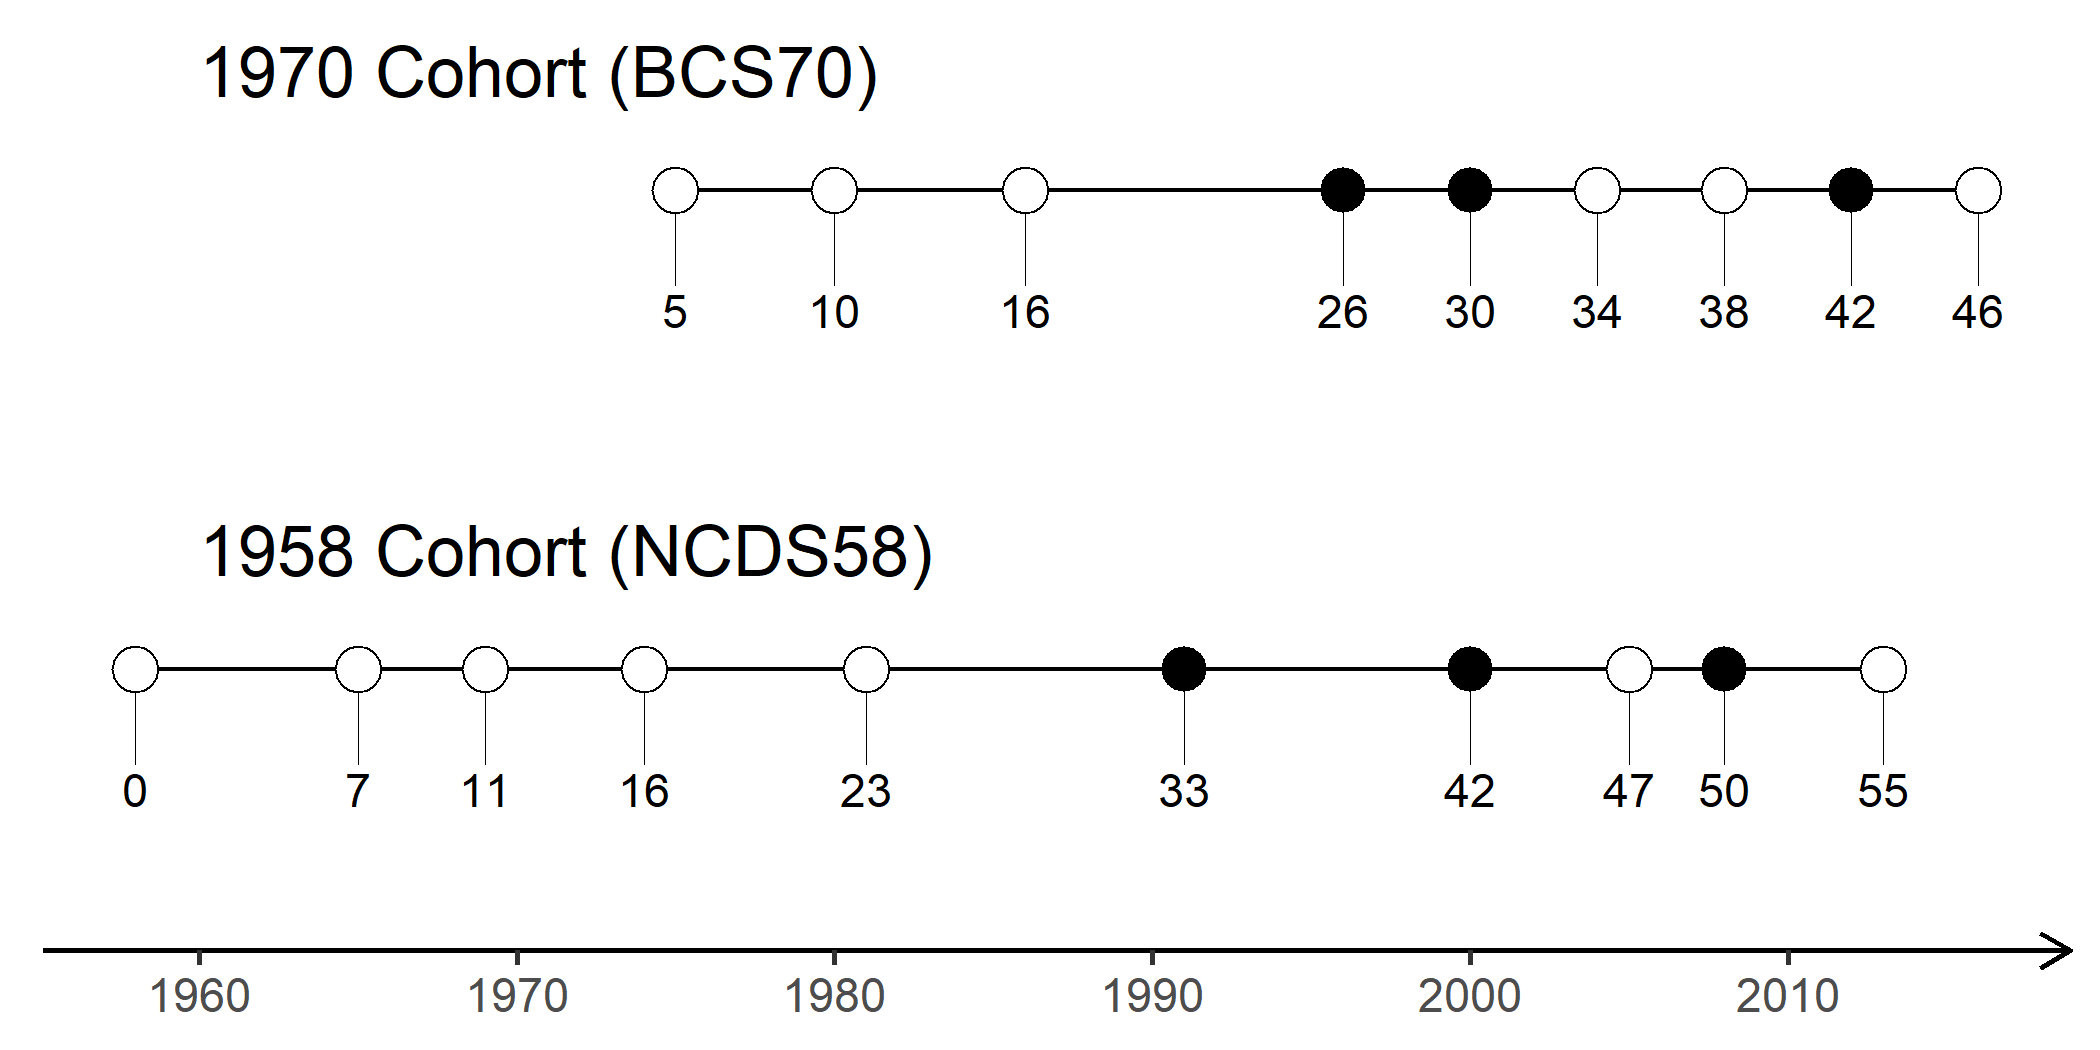
\includegraphics[width=\linewidth]{chap3/graphic/data-itw-values.png}
    \hrulefill
	\vspace{-3em}
	\justify\singlespacing\footnotesize{\textit{Notes:} This figure presents the timing of interviews for the NCDS58 and BCS70 cohorts. Circles correspond to interviews and numbers under them indicate the age of cohort members during this interview. Full circles correspond to interviews for which attitudes can be derived. The horizontal arrow at the bottom of the figure represents the years.}
\end{figure}
% Attitudes available
The full circles on the figure indicate interviews from which values can be derived, thus I will focus on those years for the remaining of the paper.
% Periods definition
I define four periods according to the decade in which individuals belong, i.e. their twenties, thirties, forties, or fifties.
% BCS periods
For the BCS70 cohort, I refer to period 1 for the interview at the age of 26, to period 2 for the one at 30, and to period 3 for the one at 42.
% NCDS periods
For the NCDS58 cohort, periods start at period 2 for the interview at the age of 33, then period 3 corresponds to the one at 42, and period 4 refers to the one at 50.

% Attrition ?
One of the main issues with cohort studies is attrition. 
% Either missing interviews OR lose them
Cohort members do not participate at every interview and therefore some individuals are either missing at some interviews or lost definitely at some point.
%
Table \ref{chap3-tab:data-resp} presents the responses rates by periods of interest.
% Table to show attrition
\begin{table}[!tb]
    \centering
    \caption{Number of individuals and response rates by periods.}
    \label{chap3-tab:data-resp}
    \begin{threeparttable}
        \setlength{\tabcolsep}{15pt}
        
\begin{tabular}{lrr}
\toprule
  & \multicolumn{1}{c}{BCS} & \multicolumn{1}{c}{NCDS}\\
\midrule
Initial & 19,006 (100\%) & 17,885 (100\%)\\
\midrule
Period 1 & 9,003 (47.4\%) & \\
Period 2 & 11,261 (59.2\%) & 11,469 (64.1\%)\\
Period 3 & 9,841 (51.8\%) & 11,419 (63.8\%)\\
Period 4 &  & 9,790 (54.7\%)\\
\midrule
All & 6,115 (32.2\%) & 8,107 (45.3\%)\\
\bottomrule
\end{tabular}

        \begin{tablenotes}[flushleft]
            \footnotesize{\item \textit{Notes}: Response rates between parentheses. The last row corresponds to individuals who have been interviewed at all periods.}
        \end{tablenotes}
    \end{threeparttable}
\end{table}
%
The second-period interview is the one with the greater response rate, i.e. 64.1\% for the NCDS58 cohort and 59.2\% for the BCS70 one. This latter interview, when BCS70 cohort members are 30, has been conducted at the same time as the third-period interview for the NCDS58 cohort, when they are 42, so in the year 2000. Thus, they share the same set of variables.

\subsection{Motivational types of values}

% Attitudes from statements
I derive values from individuals' answers to statements about their attitudes.\footnote{In social psychology, an attitude toward an object---such as a statement---corresponds to emotions, beliefs, and behaviors toward this particular object.} At each interview, cohort members answer to statements using a 5-level scale (strongly disagree / disagree / neither agree nor disagree / agree / strongly agree). I attribute them a score for each statement between -2 and 2 according to the answer.

% Group statement by categories
These statements cover several attitudes and can be grouped into categories (in alphabetical order): Anti-Racism (AR), Authority (A), Children (C), Environment (E), Inequality Aversion (IA), Information Technology (IT), Learning (L), Morale (MOR), Political Cynicism (PC), Work-Ethic (WE), and Working Mother (WM). 
The full list of statements are reported in appendix \ref{chap3-statement}. Some examples of statements are the following:
\begin{table}[!h]
    % \footnotesize
    \renewcommand*{\arraystretch}{1.5}
	\begin{tabular}{rl}
    (A2)    & \textit{For some crimes the death penalty is the most appropriate sentence};\\
    (MOR3)  & \textit{Couples who have children should not separate};\\
    (PC1)   & \textit{None of the political parties would do anything to benefit me};\\
    (WE1)   & \textit{Having almost any job is better than being unemployed}.
    \end{tabular}
\end{table}

% Compute the average score
\noindent I compute the average score within each attitude category for each individual at each period. Thus, each individual has a score for each attitude in each period. Then, I standardize each attitude score at the cohort and period level. Thus, each individual belongs to a cohort and has, for each period, a standardized score for each attitude that is relative to her cohort in a given period.

%
Nonetheless, the number of available statements depends on the cohort and the period. Table \ref{chap3-tab:data-available-short} summarizes the number of available statements at each interview.
\begin{table}[!tb]
    \centering
    \caption{Number of available statements at each interview}
    \label{chap3-tab:data-available-short}
    \begin{threeparttable}
        \setlength{\tabcolsep}{12pt}
        \begin{tabular}{lrrrrrr}
\toprule
\multicolumn{1}{c}{} & \multicolumn{3}{c}{BCS70} & \multicolumn{3}{c}{NCDS58} \\
\cmidrule(l{3pt}r{3pt}){2-4} \cmidrule(l{3pt}r{3pt}){5-7}
Attitude & 26 & 30 & 42 & 33 & 42 & 50\\
\midrule
Authority & 4 & 6 & 3 & 6 & 6 & 3\\
Anti-Racism &  & 5 & 2 & 5 & 5 & 3\\
Children &  & 4 & 2 & 2 & 4 & \\
Environment &  & 3 & 2 & 3 & 3 & 3\\
Inequality Aversion & 1 & 7 & 5 & 7 & 7 & 3\\
Info. Techno. &  & 4 &  &  & 4 & \\
Learning &  & 4 &  &  & 4 & \\
Morale & 3 & 6 & 3 & 6 & 6 & 3\\
Political Cynicism & 3 & 3 & 3 & 3 & 3 & 3\\
Work Ethic & 2 & 3 & 3 & 3 & 3 & 3\\
Working Mother &  & 5 & 2 &  & 5 & \\
\bottomrule
\end{tabular}
        \begin{tablenotes}[flushleft]
            \footnotesize{\item \textit{Notes}: This table presents the number of available statements in each attitudes at each age for the NCDS58 and BCS70 cohorts. Details on statements are reported in the appendix, see tables \ref{chap3-tab:statement-split-1}, \ref{chap3-tab:statement-split-2} and \ref{chap3-tab:statement-split-3} in appendix \ref{chap3-statement}.}
        \end{tablenotes}
        \end{threeparttable}
\end{table}
%
Thus, interviews do not necessarily share the same set of statements, except when the BCS70 cohort is 30 and the NCDS58 cohort is 42 because interviews were performed using the same questionnaires.

I derive motivational types of values from these attitude scores. I focus on the five attitudes that are available in all interviews in order to have the same baseline for each period of both cohorts. These attitudes are Authority (A), Inequality Aversion (IA), Morale (MOR), Political Cynicism (PC), and Work Ethic (WE).

%
I use a Principal Component Analysis (PCA) to transform the 5-dimension attitudes into the two-dimension motivational types of values. PCA increases the interpretability of vectors while minimizing the information loss. By focusing on the two first components, which are orthogonal by the construction of the PCA, I can interpret them as the two main values that discriminate and, therefore, characterize individuals in their attitudes. 

The other principal components act as residuals to some extent. Although they might be incorporated into the analysis, Proposition \ref{chap3-prp:relevant} states that a value needs to be sufficiently discriminatory between groups in order to be relevant in the group membership decision. The two first principal components capture more than 50\% of the explained variance in attitudes, which makes the discriminatory power of the other principal components less relevant.
% \footnote{PCA allows to determine values by summarizing attitudes through dimension reduction which reduces the noise in attitudes, hence, this noise is relegated to the unused components that explain the smaller part of the variance and are not relevant.} Therefore, I focus on the two first components.

%
I perform PCA at the cohort and period level. Figure \ref{chap3-fig:data-pca-v5} presents the eigenvectors of the two first principal components.
\begin{figure}[!tb]
    \centering
    \caption{Eigenvectors of the two first principal components}
    \label{chap3-fig:data-pca-v5}
    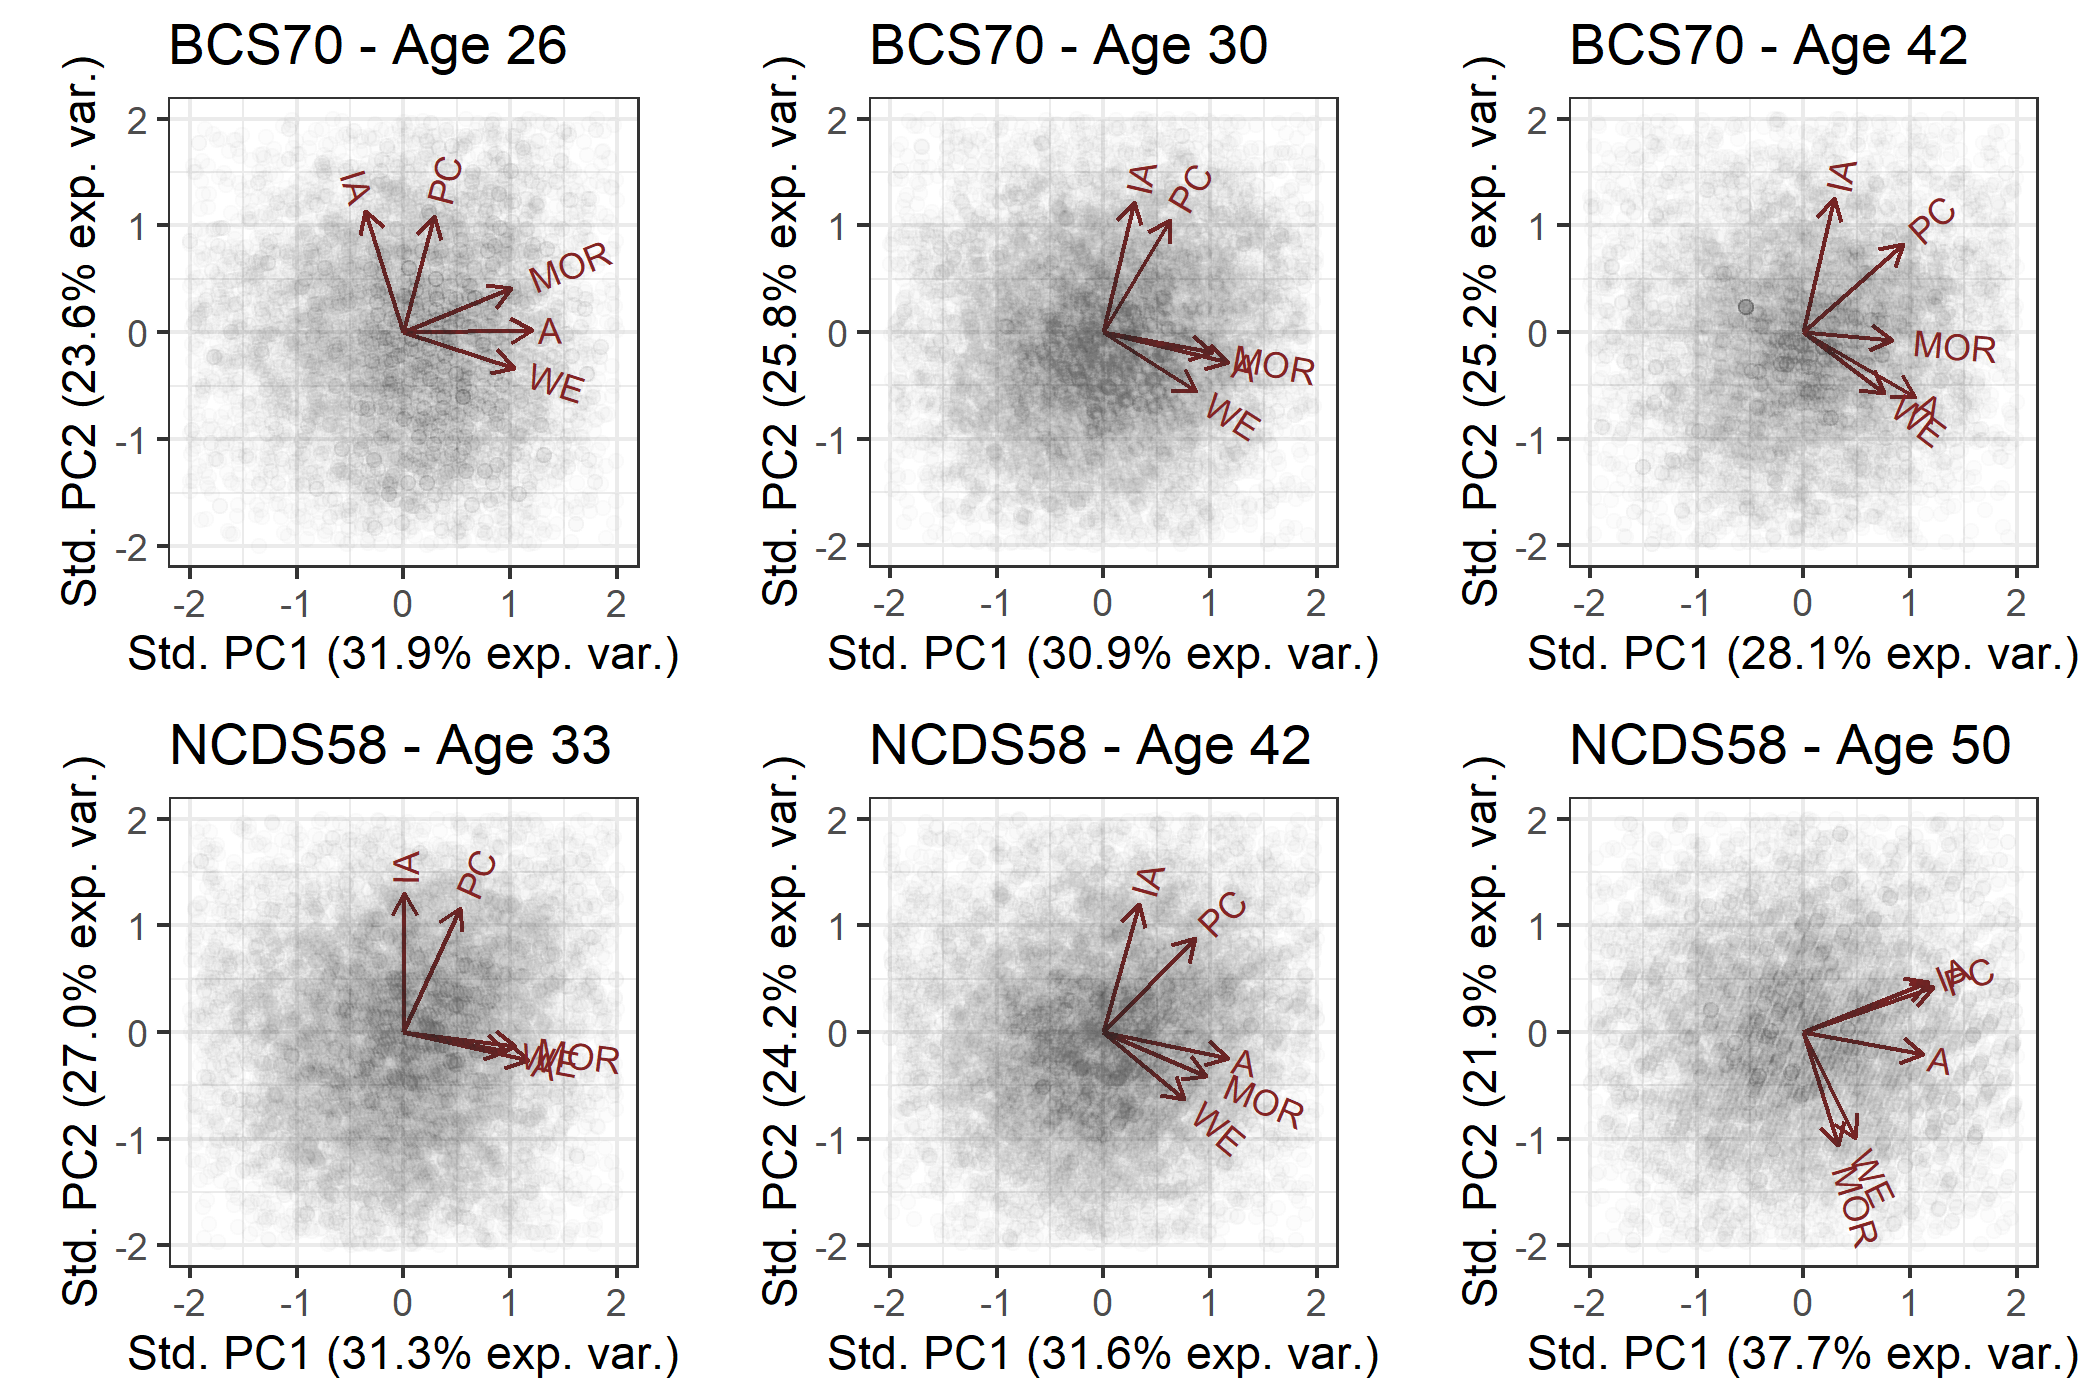
\includegraphics[width=\linewidth]{chap3/graphic/pca-v5.png}
    \hrulefill
	\vspace{-3em}
	\justify\singlespacing\footnotesize{\textit{Notes:} This figure presents the eigenvectors of the two first principal components. Details on the eigenvectors are available in tables \ref{chap3-tab:pca-v5-BCS70} and \ref{chap3-tab:pca-v5-NCDS58}, respectively for the BCS70 and NCDS58 cohorts. Attitudes are Authority (A), Inequality Aversion (IA), Morale (MOR), Political Cynicism (PC) and Work Ethic (WE).}
\end{figure}
Links between attitudes are fairly stable across cohorts and periods. These principal components explain more than 50\% of the variance in attitudes. I interpret both of them as the two-dimensional structure of universal motivational types of values, as introduced by \citet{Schwartz1992Universals, Schwartz2012Overview}---see figure \ref{chap3-fig:schwartz} in the appendix.

% PC1
Focusing on the first principal component (PC1), the x-axis directions of vectors highlight attitudes that characterize \textit{conservatism} which is the preference for stability, security, tradition, and conformity. In the data, they reflect a taste for attitudes about Authority, Morale, and Work Ethic. Thus, the dimension that discriminates the most between individuals is \textit{conservatism} (versus \textit{progressivism}).
% PC2
The second principal component (PC2) is orthogonal to the previous dimension of values at the cohort-period level. Focusing on the y-axis directions of vectors, they indicate attitudes that characterize \textit{collectivism}. This motivational type of values refers to the care and concern about others, reflecting universalism and benevolence. In the data, this value is associated with attitudes toward Political Cynicism and aversion for Inequality and Work Ethic. Therefore, the second discriminatory dimension between individuals is \textit{collectivism} (versus \textit{individualism}).\footnote{In the terms of \citet{Schwartz1992Universals}, both dimensions are respectively named conservation (versus openness-to-change) and self-transcendence (versus self-enhancement).}

% Projection
I make a projection of both principal components for all individuals at each period.  Thus, each cohort member has a Conservatism score ($Cons$) and a Collectivism score ($Coll$) at each period. By construction, both scores are standardized at the cohort-period level and \textit{orthogonal}. Thus, the values are not inter-dependent \textit{per se}. The inter-dependency arises with socio-economic characteristics---such as gender, education, etc.---once they are introduced as control variables. These covariates capture several dimensions of groups to which individuals identify, hence, it creates inter-dependency between values as they are correlated among groups.

\subsection{Groups mapping using political vote}

In my theoretical framework, the agent belongs to a group and the spillover effect occurs once the agent identifies with another group. Defining groups is therefore crucial to understand spillover effects as we expect individuals to change groups along with their values. So far, a group can be interpreted as composed of peers with whom the agent identifies in terms of values. One can think about those peers as close people such as relatives, neighbors, or colleagues; since we tend to share values with them. Nonetheless, most of the time, individuals cannot freely break off all ties with those latter as there may be direct costs. These direct costs thwart the identification of changes in group membership as they introduce noise through bonds. Thus, I cannot rely on peers to define groups.

An alternative proxy for groups is political vote. There is no direct cost in voting for one party or another at the general election, conditional on voting. In addition, political parties reflect part of individuals' values in the sense that the agent decides to identify with one party with respect to others when voting.

Figure \ref{chap3-fig:vote-v5} presents a mapping of values of the average voters for each main political party at the closest general election (GE); see table \ref{chap3-tab:data-vote} in appendix \ref{chap3-details} for the shares of vote in both cohorts.
\begin{figure}[!tb]
    \centering
    \caption{Average values according to political vote}
    \label{chap3-fig:vote-v5}
    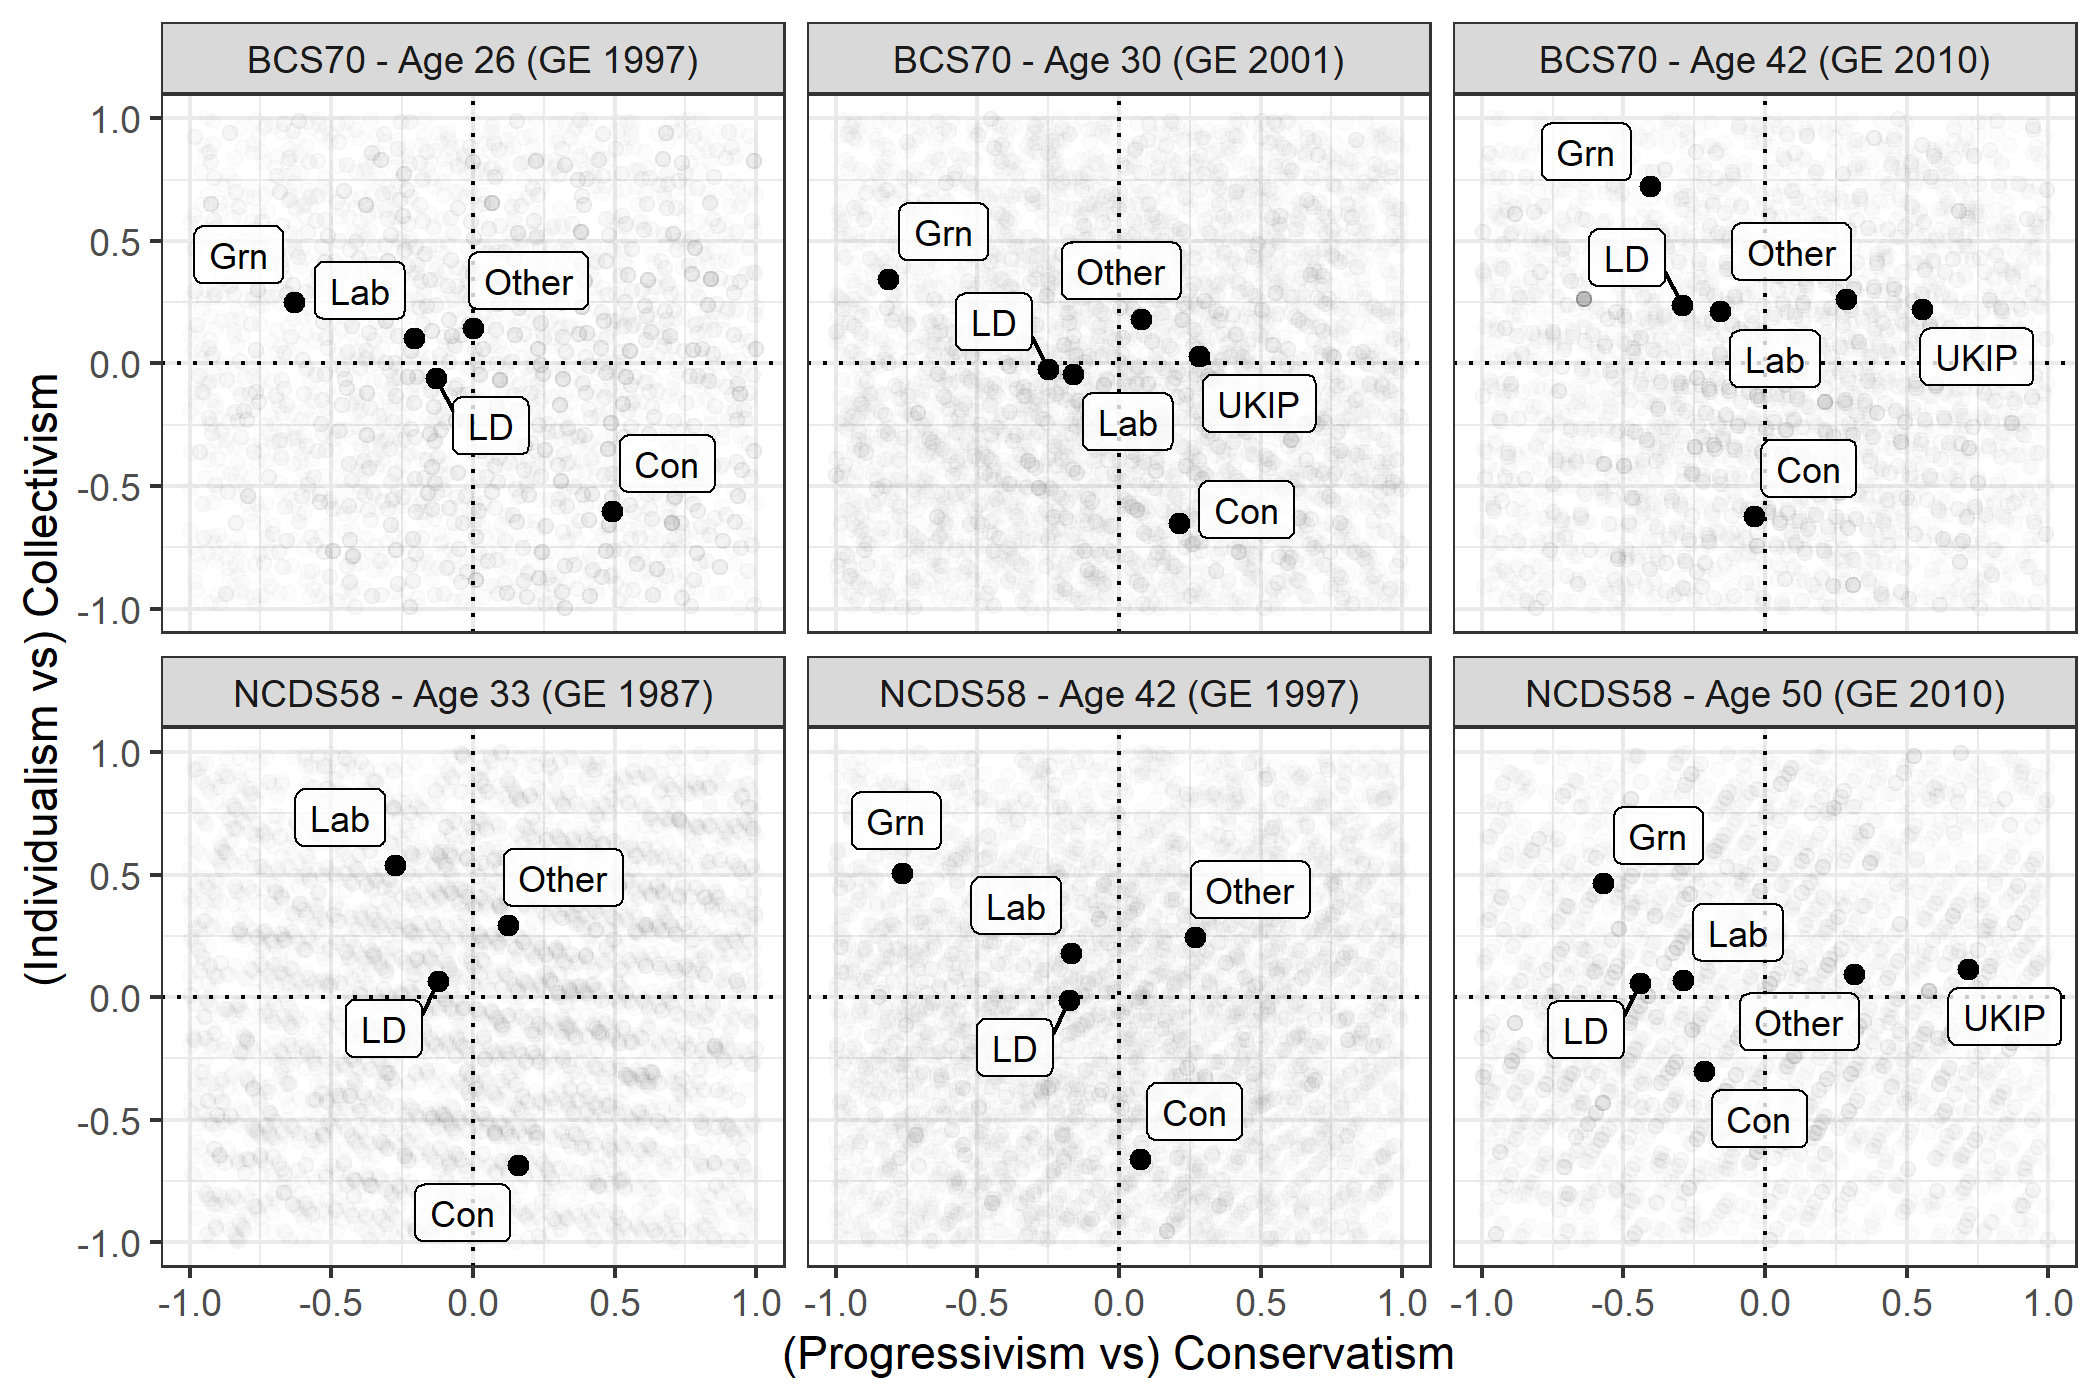
\includegraphics[width=\linewidth]{chap3/graphic/vote-v5.png}
    \hrulefill
	\vspace{-3em}
	\justify\singlespacing\footnotesize{\textit{Notes:} This figure presents the mapping of average scores in conservatism and collectivism according to political voting in General Elections (GE). Political parties are (in alphabetical order): Conservative (Con), Green (Grn), Labour (Lab), Liberal Democrat (LD), and UK Independence Party (UKIP). Other encompasses all other parties, blank votes and abstention.}
\end{figure}
% 1987 GE
The bottom-left panel represents the mapping of values in the 1987 General Election for which only the NCDS58 cohort voted at age 33. Positioning of the two main UK political parties is consistent: Labour (Lab) voters are progressive and collectivist, whereas Conservative (Con) voters are conservative and individualist. The Liberal Democrats (LD) provides an in-between the Labour and Conservative parties.\footnote{Note that the Liberal Democrats party only appeared in 1988 as the merge of the SDP–Liberal Alliance that was running into general elections in 1987. For the ease of exposition, I refer to the SDP–Liberal Alliance in 1987 as the Liberal Democrats.}
Other encompasses all other parties, blank votes, and abstention.
% 1997 GE
The top-left and bottom-mid panels correspond to the 1997 General Election. The Green party (Grn) emerged and attracted voters with progressive and collective values. The overall structure of values and voting is stable across cohorts.
% 2001 GE
The top-mid panel shows the rise of the far-right party UKIP for the 2001 General Election. As the formation of political parties is endogenous, it is unsurprising that it emerged in an area where there was no political supply.
% 2010 GE
Both right panels depict the political mapping for the 2010 general election. The average political voters of the BCS70 cohort are more spread along the collectivism axis, while those in the older cohort are rather spread on the conservatism axis.

Positionings of political parties relative to each other are consistent---over time and across cohorts---on the two-dimensional values' space. Thus, I consider the political vote of individuals as a proxy of their group membership in the remaining of the empirical analysis. This proxy helps understand how individuals start to identify with other groups after life-changing events.

\subsection{Life-changing events}

We are interested in life events that generate information shocks on conservatism ($Cons$) or collectivism ($Coll$) in order to show whether there exist spillover effects or not. The type of life events that I have to consider to test this hypothesis requires two properties: \textit{exogeneity} and \textit{non-reversibility}.
On the one hand, the life event has to be exogenous so that values in the previous period do not influence the likelihood that the life event occurs. 
On the other hand, the life event has to be non-reversible. Otherwise, the probability to reverse the event is likely to be endogenous which would bias the estimate of individual's values at the time of interviews.\footnote{Note that life events that provide temporary shocks are also interesting to study. Especially if a temporary shock leads to a change in groups. In the absence of reverse shock, both---time and group---consistencies would prevent the individual to come back to her previous group's values. Thus, a sufficiently large temporary shock can have long-run consequences on individuals' values.}

In this regard, I focus on two life events that satisfy both properties, namely, \textit{to have ever had cancer} and \textit{to have a girl as first child conditional on having a baby}.
%
The former life event is exogenous in the sense that values, such as conservation and collectivism, do not affect the probability to have cancer---excluding individuals with lung cancer. It is also non-reversible as I compare individuals who have \textit{ever} had cancer with respect to those who never had one. I set the focus on the information shock related to the fact that people have known they have cancer, not on the illness \textit{per se} as someone might have one without knowing it.
Note that for the older cohort at age 50, there may be a bias when considering the effect of this life event on values. As people turn 50, they expect that their health condition will deteriorate in the coming years, thus, they may anticipate such a life event and change their values beforehand. This potential mechanism would bias my estimate toward zero as the control group---those who did not get cancer yet---anticipate and shift their values in the same direction as those who have been treated. Therefore, for this cohort at that age, my approach is likely to provide a lower bound estimate of the effect of having ever had cancer on values.

For the latter life event, I consider a sub-sample that only contains individuals who have at least one baby, hence, I compare those who had a girl as a first child with those who got a boy.
Thus, the life event is exogenous to values because the probabilities of child's sex at birth are fifty-fifty, considering that sex‐selective abortion is very rare in the UK.\footnote{
\citet{Dubuc2007Increase} argue that sex-selective abortion occurs among mothers born in India and living in Britain. They show that sex ratios at birth have always been one point lower for Asian groups in England and Wales before 1990. Although this issue raises several social and economic concerns, it does not statistically affect my results as they represent a minority in the data.} Once the baby is born, the life event is non-reversible because it has occurred and remains forever.
I do not also consider adopted children because the sex may be decided by parents and therefore linked to values and preferences (\citealt{Dahl2008Demand}). I also exclude stillborn babies because the socialization of parents with the baby does not occur.\footnote{Note that this tragic life event could also be considered as a potential life event that would deeply affect values.}

%
I only focus on the first child as fertility decisions for following children might be linked to the sex of the eldest child and values, e.g. a preference for diversity in children's birth sex. Moreover, some parents may have a boy as their first child and a girl thereafter. Some changes in values may be specific to having a girl even though she is not the first baby. Thus, this is likely to produce a lower-bound estimate and also to reduce the statistical power of effects of this life event on values.

Lastly, I study the role of unemployment on values as it is a sizeable information shock in individuals' life. Nonetheless, I cannot use it as a life event to show the existence of spillover effects among values because it does not satisfy both properties. First, individuals change their activity status quite often and, therefore, the effect of unemployment on values is all the time affected by these changes in status. Second, the likelihood to be unemployed is clearly endogenous to values. For instance, one might argue that individuals with high work ethic, hence high conservatism and high individualism, have a lower probability to be unemployed as they are less likely to quit their job with respect to people with low work ethic.

\subsection{Variables and summary statistics}

%%%%% LIFE EVENT VARIABLES %%%%%
For life events, I focus on three of them: to have had a girl as a first child, to have ever had cancer, and to have ever been unemployed. $GirlFirst$ is a dummy variable that equals one if the sex of the first child is female, and zero if it is a male. $GotCancer$ is also a dummy variable that equals one if the individual has ever had cancer by the time of the interview. $BeenUnemp$ is a dummy variable that equals one if the individual has ever been unemployed at least one month by the time of the interview. 
% Activity history
Activity status is derived from the full activity histories to the nearest month since cohort members are 16 years old. These data are available for all cohort members until the last interview they have participated in. When individuals were missing in previous interviews, interviewers asked them about their activities during the period until then.

%%%%% SOCIO-ECONOMIC CHARACTERISTICS %%%%%
I consider several socio-economic characteristics as control variables that will introduce the inter-dependency between values. Among them, I use the sex at birth of cohort members and their level of education based on the highest academic qualification they obtained. $Female$ is a dummy variable that equals one if the cohort member is born as a female. I regroup education levels into three categories that characterize primary, secondary, and tertiary education levels ($Educ$). 

%%%%% SUMMARY STATISTICS %%%%%
Table \ref{chap3-tab:data-statdesc} presents the descriptive statistics for the NCDS58 and BCS70 cohorts. Both cohorts contain respectively 30,552 and 27,906 observations. Period variables corresponds to dummy variables to determine the decade in which individuals are.
\begin{table}[!tb]
    \centering
    \caption{Summary statistics}
    \label{chap3-tab:data-statdesc}
    \begin{threeparttable}
        \setlength{\tabcolsep}{5pt}
        
\begin{tabular}{lrrrrrrrrrr}
\toprule
\multicolumn{1}{c}{} & \multicolumn{5}{c}{NCDS58 - N = 30,552} & \multicolumn{5}{c}{BCS70 - N = 27,906} \\
\cmidrule(l{3pt}r{3pt}){2-6} \cmidrule(l{3pt}r{3pt}){7-11}
Variable & Mean & SD & Min & Max & NA & Mean & SD & Min & Max & NA\\
\midrule
Period 1 - Twenties &  &  &  &  &  & 0.31 & 0.46 & 0 & 1 & 0\\
Period 2 - Thirties & 0.35 & 0.48 & 0 & 1 & 0 & 0.40 & 0.49 & 0 & 1 & 0\\
Period 3 - Forties & 0.37 & 0.48 & 0 & 1 & 0 & 0.29 & 0.45 & 0 & 1 & 0\\
Period 4 - Fifties & 0.28 & 0.45 & 0 & 1 & 0 &  &  &  &  & \\
Female & 0.51 & 0.50 & 0 & 1 & 0 & 0.53 & 0.50 & 0 & 1 & 0\\
Education - Primary & 0.62 & 0.49 & 0 & 1 & 0 & 0.52 & 0.50 & 0 & 1 & 0\\
Education - Secondary & 0.19 & 0.39 & 0 & 1 & 0 & 0.19 & 0.39 & 0 & 1 & 0\\
Education - Tertiary & 0.20 & 0.40 & 0 & 1 & 0 & 0.29 & 0.46 & 0 & 1 & 0\\
Girl First & 0.49 & 0.50 & 0 & 1 & 7199 & 0.48 & 0.50 & 0 & 1 & 14789\\
Got Cancer & 0.03 & 0.16 & 0 & 1 & 0 & 0.01 & 0.12 & 0 & 1 & 0\\
Been Unemployed & 0.34 & 0.48 & 0 & 1 & 0 & 0.21 & 0.41 & 0 & 1 & 0\\
\bottomrule
\end{tabular}

        \begin{tablenotes}[flushleft]
            \footnotesize{\item \textit{Notes}: This table presents the descriptive statistics of variables used in the study. Values and attitudes are not displayed in this table as they are standardized.}
        \end{tablenotes}
    \end{threeparttable}
\end{table}

    
    \section{Empirical evidence} \label{chap3-empirics}
    % What do we do here?
The empirical work aims to investigate the presence of spillover effects across values and how they behave. I proceed in several steps. First, I investigate the effect of both exogenous life events, which characterize the information shocks, on conservatism, collectivism, and group membership, but independently. I observe that only conservatism is affected. Second, I show the presence of spillover effects on collectivism by instrumenting conservative values with the life event. Third, I raise the issue of the two-sided effect in the case of unemployment as unemployment does affect both values at the same time, hence, the identification using instrumental variables does not hold in this setting. 

\subsection{Effect of life events on values}

I estimate \textit{independently} with OLS the effect of the life event $z\in Z=\{GotCancer$, $GirlFirst$, $BeenUnemp\}$ on value $v\in V=\{Cons$, $Coll\}$ for an individual $i$ in period $t$ with the following equation:
\begin{equation}\label{chap3-eq:est-indep}
    v_{it} = \alpha + \beta \times z_{it} + \eta \times v_{i,t-1} + X_{i} \delta + u_{it}
\end{equation}
where $X$ are control variables including gender, education, along with period and cohort fixed effects. 

Table \ref{chap3-tab:reg-v5-raw-all-short} summarizes the coefficients.
\begin{table}[!tb]
    \centering
    \caption{Effect of life events on values}
    \label{chap3-tab:reg-v5-raw-all-short}
    % \resizebox*{\textwidth}{!}{
    \begin{threeparttable}
        \setlength{\tabcolsep}{0pt}
        \begin{tabular}{l D{.}{.}{5.5} D{.}{.}{5.5} D{.}{.}{5.5} D{.}{.}{5.5} D{.}{.}{5.5} D{.}{.}{5.5}}
\toprule
 & \multicolumn{6}{c}{Linear regression - OLS} \\
\cmidrule(lr){2-7}
 & \multicolumn{2}{c}{GirlFirst} & \multicolumn{2}{c}{GotCancer} & \multicolumn{2}{c}{BeenUnemp} \\
\cmidrule(lr){2-3}\cmidrule(lr){4-5}\cmidrule(lr){6-7}
 & \multicolumn{1}{c}{(Cons)} & \multicolumn{1}{c}{(Coll)} & \multicolumn{1}{c}{(Cons)} & \multicolumn{1}{c}{(Coll)} & \multicolumn{1}{c}{(Cons)} & \multicolumn{1}{c}{(Coll)} \\
\midrule
Life event    & 0.03^{**}  & 0.00       & 0.09^{***} & 0.02       & 0.02^{*}   & 0.18^{***} \\
              & (0.01)     & (0.01)     & (0.03)     & (0.03)     & (0.01)     & (0.01)     \\
Value$_{t-1}$ & 0.54^{***} & 0.49^{***} & 0.56^{***} & 0.50^{***} & 0.56^{***} & 0.49^{***} \\
              & (0.01)     & (0.01)     & (0.00)     & (0.00)     & (0.00)     & (0.00)     \\
\midrule
R$^2$ & \multicolumn{1}{c}{0.37} & \multicolumn{1}{c}{0.26} & \multicolumn{1}{c}{0.39} & \multicolumn{1}{c}{0.27} & \multicolumn{1}{c}{0.39} & \multicolumn{1}{c}{0.27}\\
Adj. R$^2$ & \multicolumn{1}{c}{0.37} & \multicolumn{1}{c}{0.26} & \multicolumn{1}{c}{0.39} & \multicolumn{1}{c}{0.27} & \multicolumn{1}{c}{0.39} & \multicolumn{1}{c}{0.27}\\
Num. obs. & \multicolumn{1}{c}{23354} & \multicolumn{1}{c}{23354} & \multicolumn{1}{c}{32885} & \multicolumn{1}{c}{32885} & \multicolumn{1}{c}{32885} & \multicolumn{1}{c}{32885}\\
\bottomrule
\end{tabular}

        \begin{tablenotes}[flushleft]
            \footnotesize{\item \textit{Notes}: $^{***}p<0.01$; $^{**}p<0.05$; $^{*}p<0.1$. Standard errors between parentheses. Control variables include gender, education (primary, secondary, tertiary), cohort fixed effects and period fixed effects. Male in the NCDS cohort in his forties with primary education as the reference group. GirlFirst and GotCancer are the life events. In GirlFirst regressions, parents who have had a boy as a first child are the reference group. In GotCancer regressions, individuals who never had a cancer are the reference group. In BeenUnemp, individuals who have never been unemployed are the reference group. Table \ref{chap3-tab:reg-v5-raw-all-long} in the appendix presents all the coefficients.}
        \end{tablenotes}
    \end{threeparttable}
    % }
\end{table}
% Life event row
For both life events, having a girl as a first child and having ever had cancer, the coefficients are positive and significant in both (Cons) columns; while they are not significant in (Coll) ones.
Parents who have had a girl as a first child, instead of a boy, tend to hold more conservative values, about 0.03 standard deviation, without any statistical difference in their collectivism.
Individuals who have ever had cancer seem to be more conservative, by 0.09 standard deviation, although they do not differ from others in terms of collectivism versus individualism.
For having ever been unemployed, the associated coefficients are both significant and positive.
Individuals who have ever been unemployed tend to be more conservative and collectivist, by respectively 0.02 and 0.18 standard deviation.

% Value t-1 row
Coefficients associated with the lag of the value lie around 0.55 standard deviation for conservatism and around 0.49 standard deviation for collectivism. This pattern indicates that conservative values are more correlated over periods than collectivist values. In terms of the theoretical framework, it provides evidence that time consistency may be more important for conservatism with respect to collectivism.

\subsection{Values change and group membership}

As we observe that people affected by life-changing events tend to hold different values, we, hence, look at their likelihood to change their group membership. Let $p_s$ be the probability to vote for a political party $s\in\{Con,$ $Grn,$ $Lab,$ $LD,$ $UKIP\}$. Thus, we can estimate these probabilities relative to the probability to vote for the $Other$ category $p_O$---which encompasses all other parties, blank votes, and abstention. I estimate the following multinomial logistic regression:
\begin{equation}\label{chap3-eq:est-multi}
    \log\left(\frac{p_s}{p_O}\right) = \pi_{s} + \phi_{1s} \Delta Cons_t + \phi_{2s} \Delta Coll_t + \eta_{1s} Cons_{t-1} + \eta_{2s} Coll_{t-1} + \gamma_{s} X,
\end{equation}
where $\Delta v_t\equiv v_t - v_{t-1}$ are the changes in conservatism and collectivism, which are conditional on individuals' values in previous period, i.e. $Cons_{t-1}$ and $Coll_{t-1}$, and also conditional on the political party for which the individual voted at the previous general election. The latter variable is included in control variables $X$ along with gender, education, cohort and period fixed effects.

Table \ref{chap3-tab:reg-v5-raw-vote-short} summarizes the coefficients. 
\begin{table}[!tb]
    \centering
    \caption{Effect of values change on the group membership}
    \label{chap3-tab:reg-v5-raw-vote-short}
    \begin{threeparttable}
        \begin{tabular}{l D{.}{.}{5.5} D{.}{.}{5.5} D{.}{.}{5.5} D{.}{.}{5.5} D{.}{.}{5.5}}
\toprule
 & \multicolumn{5}{c}{Multinomial logit - Dep. var.: Vote} \\
\cmidrule(lr){2-6}
 & \multicolumn{1}{c}{(Con)} & \multicolumn{1}{c}{(Grn)} & \multicolumn{1}{c}{(Lab)} & \multicolumn{1}{c}{(LD)} & \multicolumn{1}{c}{(UKIP)} \\
\midrule
$\Delta\text{Cons}_t$    & -0.06^{***} & -0.19^{***} & -0.17^{***} & -0.10^{***} & 0.26^{***}  \\
                         & (0.02)      & (0.06)      & (0.02)      & (0.02)      & (0.05)      \\
$\Delta\text{Coll}_t$    & -0.37^{***} & 0.17^{***}  & -0.14^{***} & -0.06^{**}  & -0.01       \\
                         & (0.02)      & (0.06)      & (0.02)      & (0.02)      & (0.05)      \\
$\text{Cons}_{t-1}$      & -0.03       & -0.39^{***} & -0.23^{***} & -0.23^{***} & 0.23^{***}  \\
                         & (0.02)      & (0.05)      & (0.02)      & (0.02)      & (0.05)      \\
$\text{Coll}_{t-1}$      & -0.69^{***} & 0.21^{***}  & -0.05^{***} & -0.08^{***} & -0.03       \\
                         & (0.02)      & (0.06)      & (0.02)      & (0.02)      & (0.06)      \\
$\text{Vote}_{t-1}$ &  2.25^{***}   &  3.26^{***}   &  2.69^{***}   &  2.20^{***}   &  3.07^{***}  \\
  &  (0.05)       &  (0.23)       &  (0.06)       &  (0.04)       &  (0.42)      \\
\midrule
Num. obs. & \multicolumn{1}{c}{32885} & \multicolumn{1}{c}{32885} & \multicolumn{1}{c}{32885} & \multicolumn{1}{c}{32885} & \multicolumn{1}{c}{32885}\\
\bottomrule
\end{tabular}

        \begin{tablenotes}[flushleft]
            \footnotesize{\item \textit{Notes}: $^{***}p<0.01$; $^{**}p<0.05$; $^{*}p<0.1$. Standard errors between parentheses. Control variables include gender, education (primary, secondary, tertiary), cohort fixed effects and period fixed effects. Male in the NCDS cohort in his forties with primary education as the reference group. GirlFirst and GotCancer are the life events. In GirlFirst regressions, parents who have had a boy as a first child are the reference group. In GotCancer regressions, individuals who never had a cancer are the reference group. 
            % Multinomial
            The baseline outcome of the multinomial logistic regression is the vote for Other (encompassing all other parties, blank votes, and abstention). $\text{Vote}_{t-1}$ corresponds to the effect of having voted for the same party in the previous period.
            Table \ref{chap3-tab:reg-v5-IV-GFvote} and \ref{chap3-tab:reg-v5-IV-GCvote} in the appendix present all the coefficients for both life events.}
        \end{tablenotes}
    \end{threeparttable}
\end{table}
These coefficients provide the log odds of voting for the political party $(s)$ relative to the baseline outcome (voting for $Other$). The signs of those coefficients have to be compared with the relative position of political parties with respect to Other category, as depicted in figure \ref{chap3-fig:vote-v5}. 

To derive the effect of values' changes on the odds of voting for one party with respect to another one, we take the exponential of the difference between both coefficients.
For instance, a one-standard-deviation increase in conservatism raises the odds to vote for the Conservatives with respect to the Labour party by 12\%, but it also reduces the odds to vote for the Conservatives with respect to UKIP by 27\%.
Similarly, a one-standard-deviation increase in collectivism raises the odds to vote for the Labour party with respect to its historical rival by 26\%.\footnote{These coefficients are obtained by taking the exponential of the difference between both associated coefficients, respectively, $\exp(-0.06-(-0.17)) = 1.12$, $\exp(-0.06-0.26) = 0.73$ and $\exp(-0.14-(-0.37)) = 1.26$.}

Changes in values are associated with changes in the likelihood to vote for the political parties, hence, with changes in the probability to identify with a new group. An increase in conservative values is associated with a rise in the probability to vote for right-wing and far-right parties, while an increase in collectivist values relates to individuals being more likely to vote for left-wing parties.

\subsection{Spillover effects}\label{chap3-sec:spillover}

To test the existence of spillover effects, I estimate instrumental variable (IV) regressions using two-stage least squares (2SLS). I assume that the information shock associated to the life event ($z$) affects the conservative value ($Cons$) but not the collectivism ($Coll$). Thus, by instrumenting $Cons_t$ with $z$---conditional on $Cons_{t-1}$---in a first stage, I am able to test whether there is spillover effect in the second stage in which I regress $Coll_t$ on the predicted $Cons_t$---conditional on $Coll_{t-1}$. The two stages of the 2SLS estimate can be written as:
\begin{align}
    Cons_{it} &= \alpha_1 + \beta_1 \times z_{it} + \eta_1 \times Cons_{i,t-1} + X_{i} \delta_1 + \varepsilon_{it}, \label{chap3-emp:iv-stage1} \tag{IV - Stage 1}\\
    Coll_{it} &= \alpha_2 + \beta_2 \times \widehat{Cons}_{it} + \eta_2 \times Coll_{i,t-1} + X_{i} \delta_2 + u_{it}, \label{chap3-emp:iv-stage2} \tag{IV - Stage 2}
\end{align}
where $\widehat{Cons}$ are the predicted $Cons$ and $X$ are control variables including gender, education, along with period and cohort fixed effects.

% Results
Table \ref{chap3-tab:reg-v5-IV-GFGC-short} summarizes the coefficients for the IV regressions.
\begin{table}[!tb]
    \centering
    \caption{IV Estimate of the spillover effect}
    \label{chap3-tab:reg-v5-IV-GFGC-short}
    % \resizebox*{\textwidth}{!}{
    \begin{threeparttable}
        \begin{tabular}{l D{.}{.}{5.5} D{.}{.}{5.5} D{.}{.}{5.5} D{.}{.}{5.5}}
\toprule
 & \multicolumn{4}{c}{IV regression - 2SLS} \\
\cmidrule(lr){2-5}
 & \multicolumn{2}{c}{GirlFirst} & \multicolumn{2}{c}{GotCancer} \\
\cmidrule(lr){2-3}\cmidrule(lr){4-5}
 & \multicolumn{1}{c}{(Cons)} & \multicolumn{1}{c}{(Coll)} & \multicolumn{1}{c}{(Cons)} & \multicolumn{1}{c}{(Coll)} \\
\midrule
Life event                & 0.03^{**}  &             & 0.09^{***} &             \\
                          & (0.01)     &             & (0.03)     &             \\
$\widehat{\text{Cons}}_t$ &            & -0.32^{***} &            & -0.34^{***} \\
                          &            & (0.01)      &            & (0.01)      \\
Value$_{t-1}$             & 0.54^{***} & 0.48^{***}  & 0.56^{***} & 0.49^{***}  \\
                          & (0.01)     & (0.01)      & (0.00)     & (0.00)      \\
\midrule
R$^2$ & \multicolumn{1}{c}{0.37} & \multicolumn{1}{c}{0.30} & \multicolumn{1}{c}{0.39} & \multicolumn{1}{c}{0.31}\\
Adj. R$^2$ & \multicolumn{1}{c}{0.37} & \multicolumn{1}{c}{0.30} & \multicolumn{1}{c}{0.39} & \multicolumn{1}{c}{0.31}\\
Num. obs. & \multicolumn{1}{c}{23354} & \multicolumn{1}{c}{23354} & \multicolumn{1}{c}{32885} & \multicolumn{1}{c}{32885}\\
\bottomrule
\end{tabular}

        \begin{tablenotes}[flushleft]
            \footnotesize{\item \textit{Notes}: $^{***}p<0.01$; $^{**}p<0.05$; $^{*}p<0.1$. Standard errors between parentheses. Control variables include gender, education (primary, secondary, tertiary), cohort fixed effects and period fixed effects. Male in the NCDS cohort in his forties with primary education as the reference group. GirlFirst and GotCancer are the life events. In GirlFirst regressions, parents who have had a boy as a first child are the reference group. In GotCancer regressions, individuals who never had a cancer are the reference group. Table \ref{chap3-tab:reg-v5-IV-GFGC-long} in the appendix presents all the coefficients.}
        \end{tablenotes}
    \end{threeparttable}
    % }
\end{table}
In both first-stage regressions, the information shock on conservatism due to the life event is positive and significant. To have a girl instead of a boy as a first child increases conservatism by 0.03 standard deviation, while to have ever had cancer raises conservatism by 0.09 standard deviation.

In both second-stage regressions, the spillover effect is negative and significant. For the first life event, a one-standard-deviation increase in conservatism decreases collectivism by 0.32 standard deviation; while an increase of the same magnitude for the second life event also reduces collectivism by 0.34 standard deviation. As the values associated with collectivism decrease, it means that those related to individualism increase. 

Both exogenous and irreversible life-changing events show that values changes through spillover effects. In my theoretical framework, I argue that those latter are due to a change in the group membership. To validate such a mechanism, I use the first-stage IV regression within a second-stage IV multinomial logistic regression to estimate the probability to vote for a political party. Thus, the second stage can be written as
\begin{equation}\label{chap3-eq:est-multi2}
    \log\left(\frac{p_s}{p_O}\right) = \pi^\prime_{s} + \beta_s \times \widehat{Cons}_{it} + \gamma_{s} X,
\end{equation}
where $\widehat{Cons}$ are the predicted $Cons$ from the first-stage IV regression, and $X$ are control variables including the vote in the previous general election,  gender, education, cohort and period fixed effects.

Table \ref{chap3-tab:reg-v5-IV-GFGCvote-short} summarizes the coefficients for the second-stage IV multinomial logistic regression.
\begin{table}[!tb]
    \centering
    \caption{IV Estimate of the group membership}
    \label{chap3-tab:reg-v5-IV-GFGCvote-short}
    % \resizebox*{\textwidth}{!}{
    \begin{threeparttable}
        % \setlength{\tabcolsep}{-6pt}
        \begin{tabular}{l D{.}{.}{5.5} D{.}{.}{5.5} D{.}{.}{5.5} D{.}{.}{5.5} D{.}{.}{5.5}}
\toprule
 & \multicolumn{5}{c}{IV regression - GirlFirst - Multinomial logit - Dep. var.: Vote} \\
\cmidrule(lr){2-6}
 & \multicolumn{1}{c}{(Con)} & \multicolumn{1}{c}{(Grn)} & \multicolumn{1}{c}{(Lab)} & \multicolumn{1}{c}{(LD)} & \multicolumn{1}{c}{(UKIP)} \\
\midrule
$\widehat{\text{Cons}}_t$ & 0.01        & -0.85^{***} & -0.27^{***} & -0.34^{***} & 0.18^{*}   \\
                          & (0.03)      & (0.10)      & (0.03)      & (0.04)      & (0.09)     \\
Vote$_{t-1}$ &  2.56^{***}   &  3.75^{***}   &  2.73^{***}   &  2.19^{***}   &  3.25^{***} \\
  &  (0.05)       &  (0.31)       &  (0.08)       &  (0.05)       &  (0.49)     \\
\midrule
Num. obs. & \multicolumn{1}{c}{23354} & \multicolumn{1}{c}{23354} & \multicolumn{1}{c}{23354} & \multicolumn{1}{c}{23354} & \multicolumn{1}{c}{23354}\\
\bottomrule
\toprule
 & \multicolumn{5}{c}{IV regression - GotCancer - Multinomial logit - Dep. var.: Vote} \\
\cmidrule(lr){2-6}
 & \multicolumn{1}{c}{(Con)} & \multicolumn{1}{c}{(Grn)} & \multicolumn{1}{c}{(Lab)} & \multicolumn{1}{c}{(LD)} & \multicolumn{1}{c}{(UKIP)} \\
\midrule
$\widehat{\text{Cons}}_t$ & 0.08^{***}  & -0.67^{***} & -0.24^{***} & -0.32^{***} & 0.19^{**}   \\
                          & (0.03)      & (0.07)      & (0.02)      & (0.03)      & (0.07)      \\
$\text{Vote}_{t-1}$ &  2.56^{***}   &  3.31^{***}   &  2.71^{***}   &  2.21^{***}   &  3.06^{***}  \\
  &  (0.04)       &  (0.23)       &  (0.06)       &  (0.04)       &  (0.42)      \\
\midrule
Num. obs. & \multicolumn{1}{c}{32885} & \multicolumn{1}{c}{32885} & \multicolumn{1}{c}{32885} & \multicolumn{1}{c}{32885} & \multicolumn{1}{c}{32885}\\
\bottomrule
\end{tabular}

        \begin{tablenotes}[flushleft]
            \footnotesize{\item \textit{Notes}: $^{***}p<0.01$; $^{**}p<0.05$; $^{*}p<0.1$. Standard errors between parentheses. Control variables include gender, education (primary, secondary, tertiary), cohort fixed effects and period fixed effects. Male in the NCDS cohort in his forties with primary education as the reference group. GirlFirst and GotCancer are the life events. In GirlFirst regressions, parents who have had a boy as a first child are the reference group. In GotCancer regressions, individuals who never had a cancer are the reference group. 
            % Multinomial
            The baseline outcome of the multinomial logistic regression is the vote for Other (encompassing all other parties, blank votes, and abstention). $\text{Vote}_{t-1}$ corresponds to the effect of having voted for the same party in the previous period.
            Table \ref{chap3-tab:reg-v5-IV-GFvote} and \ref{chap3-tab:reg-v5-IV-GCvote} in the appendix present all the coefficients for both life events.}
        \end{tablenotes}
    \end{threeparttable}
    % }
\end{table}
The top panel corresponds to the estimate of the relative probability to vote for each political party when the conservative values are instrumented with the $GirlFirst$ life event, whereas the bottom panel refers to the same estimate when the conservative values are instrumented with the $GotCancer$ life event.

Coefficients are fairly similar across both life events indicating that they have similar effects on the probability to vote for one political party or another. A notable exception is the $\widehat{Cons}$ in the Conservatives column (Con) that is positive but not significant in the column (Con) for the first life event, while it is significant for the second life event. Changes in voting behavior due to changes in values instrumented by life-changing events are consistent with the positioning of political parties in the two-dimensional value space depicted in figure \ref{chap3-fig:vote-v5} which provides empirical evidence of the group membership as the underlying mechanism in explaining the existence of spillover effects.

Both exogenous and irreversible life events show that spillover effects account for a third of the information shock. Nonetheless, the identification relies on the assumption that the information shock, associated with the life event, does not directly affect collectivism, i.e. $Coll \perp z$. This assumption is likely to be too strong, even for those life events.
    
    \section{Simultaneous equations model} \label{chap3-simultaneous}
    The identification of the spillover effect in the latter estimates relies on the exclusion restriction that assumes that the information shock characterized by the life event affects only one value. This assumption does not hold for any information shock that would have a two-sided effect, that is, would affect both values at the same time. Thus, I turn to simultaneous equations model which provides less restrictive assumptions for identification.

\subsection{Empirical specification}

To generalize the role of inter-dependency between values, I test the presence of spillover effects in a context where informational shocks can change both values. I consider a Simultaneous Equations Model (SEM) in which individuals' values are jointly determined, also determined by their own previous values and related to individual characteristics. Each observation consists of an individual $i$ observed in period $t$.  With two values, the structural form of the SEM can be written in matrix notation as
\begin{equation}\label{chap3-eq:emp-structural}
    V_{i,t}\Gamma = z_{i,t} \Theta + V_{i,t-1}H + X_i B + U_{i,t}
\end{equation}
where $V_{i,t} = \begin{bmatrix}Cons_t & Coll_t\end{bmatrix}$ is the matrix of dependent values in period $t$; $\Gamma = \begin{pmatrix} 1 & -\gamma_2^1 \\ -\gamma_1^2 & 1 \end{pmatrix}$ describes the relation between values; $z$ is a dummy vector which indicates whether the life event $Z$ occurred; $\Theta = \begin{pmatrix}\theta_1 \\ \theta_2 \end{pmatrix}$ captures the effect of the life event on each value; $H = \begin{pmatrix} \eta_1 & 0 \\ 0 & \eta_2 \end{pmatrix}$ describes the relation between a value in period $t$ and this same value in period $t-1$; $X$ are the individual characteristics vector including the intercept; $B$ corresponds to all coefficients that are associated to $X$; and $U$ is a matrix of the error terms.

Multiplying equation \eqref{chap3-eq:emp-structural} by the inverse of the $\Gamma$ matrix leads to the reduced form of the SEM such as
\begin{equation}
    V_{i,t} = z_{i,t}\Phi + V_{i,t-1}\Psi + X_{i}\Pi + \epsilon_{i,t}, \label{chap3-eq:emp-reduced}
\end{equation}
where $\Phi = \Theta\Gamma^{-1}$, $\Psi = H\Gamma^{-1}$, $\Pi = B\Gamma^{-1}$, and $\epsilon = U\Gamma^{-1}$. 

\textbf{Identification.}
% Assumptions for identification
The \textit{rank condition} is satisfied for both equations because the number of excluded endogenous variables in the reduced form, i.e. either $Cons_t$ or $Coll_t$, is equal to the number of excluded exogenous variables in the structural form, i.e. either $Coll_{t-1}$ or $Cons_{t-1}$. Thus, the SEM can be identified.

The identification relies on the assumption that $Cons_{t-1}$ does not affect $Coll_t$ and that $Coll_{t-1}$ does not affect $Cons_t$. As I suppose that values are permanently adjusted over time in order to have consistent values, it implies that, for instance, any change in $Coll_{t-1}$ can affect $Cons_t$ only through $Cons_{t-1}$. In addition, the \textit{order condition} is also satisfied for both equations because the number of excluded exogenous variables, i.e. $Cons_{t-1}$ and $Coll_{t-1}$, is also equal to the number of included endogenous variables, i.e. $Cons_{t}$ and $Coll_{t}$. Therefore, the SEM is exactly identified.

In the SEM, the identification assumption requires that one value is not directly affected by the lag of the other value. Thus, this assumption is less restrictive compared to the one in the IV approach in section \ref{chap3-sec:spillover} for which the information shock had to only affect one value and not the other.

\textbf{Decomposition of the total effect.}
%% Decomposition
From the reduced form equation \eqref{chap3-eq:emp-reduced}, it is possible to decompose the total effect of the life event $z$ on value $v \in V=\{v,-v\}$ as the sum of a direct effect (information shock) and an indirect effect (spillover effect), namely,
\begin{equation} \label{chap3-eq:decomp}
    \phi_v = 
    \begingroup
    \underbrace{\widetilde{\gamma}_v^v\times \theta_{v}}_\text{Direct effect}\endgroup 
    + 
    \begingroup
    \underbrace{\widetilde{\gamma}_v^{-v} \times \theta_{-v}}_\text{Indirect effect}\endgroup,
\end{equation}
where $\phi_v$ is the total effect of the life event $Z$ on value $v$, $\widetilde{\gamma}_v^v$ is the element on the diagonal of $\Gamma^{-1}$ associated to the value $v$, $\widetilde{\gamma}_v^{-v}$ is the off-diagonal element of $\Gamma^{-1}$ on the same column, while $\theta_v$ and $\theta_{-v}$ are respectively the information shocks associated to the life event $Z$ on values $v$ and $-v$ from the structural form. 

\textbf{Estimation method.}
%% ESTIMATION
I use a 2SLS estimation method to estimate the SEM. Thus, I instrument the endogenous variables of each equation with all exogenous variables from all equations. In a first step, I estimate the reduced form in equation \eqref{chap3-eq:emp-reduced} and obtain the predicted values, i.e. $\widehat{Cons}_t$ and $\widehat{Coll}_t$. 

In a second step, I estimate the structural form in equation \eqref{chap3-eq:emp-structural} in which I replace the endogenous variables with the predicted values obtained in the first step. Thus, I estimate the following system of equations:
\begin{equation*}
    \widetilde{V}_{i,t}\Gamma = z_{i,t} \Theta + V_{i,t-1}H + X_i B + U_{i,t}
\end{equation*}
where $\widetilde{V}_{i,t} = \begin{bmatrix} v_t & -\widehat{v}_t\end{bmatrix}$ in which $v_t$ is the dependent value and $-\widehat{v}_t$ encompasses the predictions of the endogenous value from the first step estimate. The 2SLS estimates of the simultaneous equations model for all the life events, which are analyzed below, are available in Appendix \ref{chap3-estimates}.

\subsection{Decomposing the total effect}

Figure \ref{chap3-fig:sem-decomp-v5-base} decomposes the total effect of each life-changing events on values between the information shock (direct effect) and the spillover effect (indirect effect).
\begin{figure}[!tb]
    \centering
    \caption{Decomposition of the effect of life-changing events on values}
    \label{chap3-fig:sem-decomp-v5-base}
    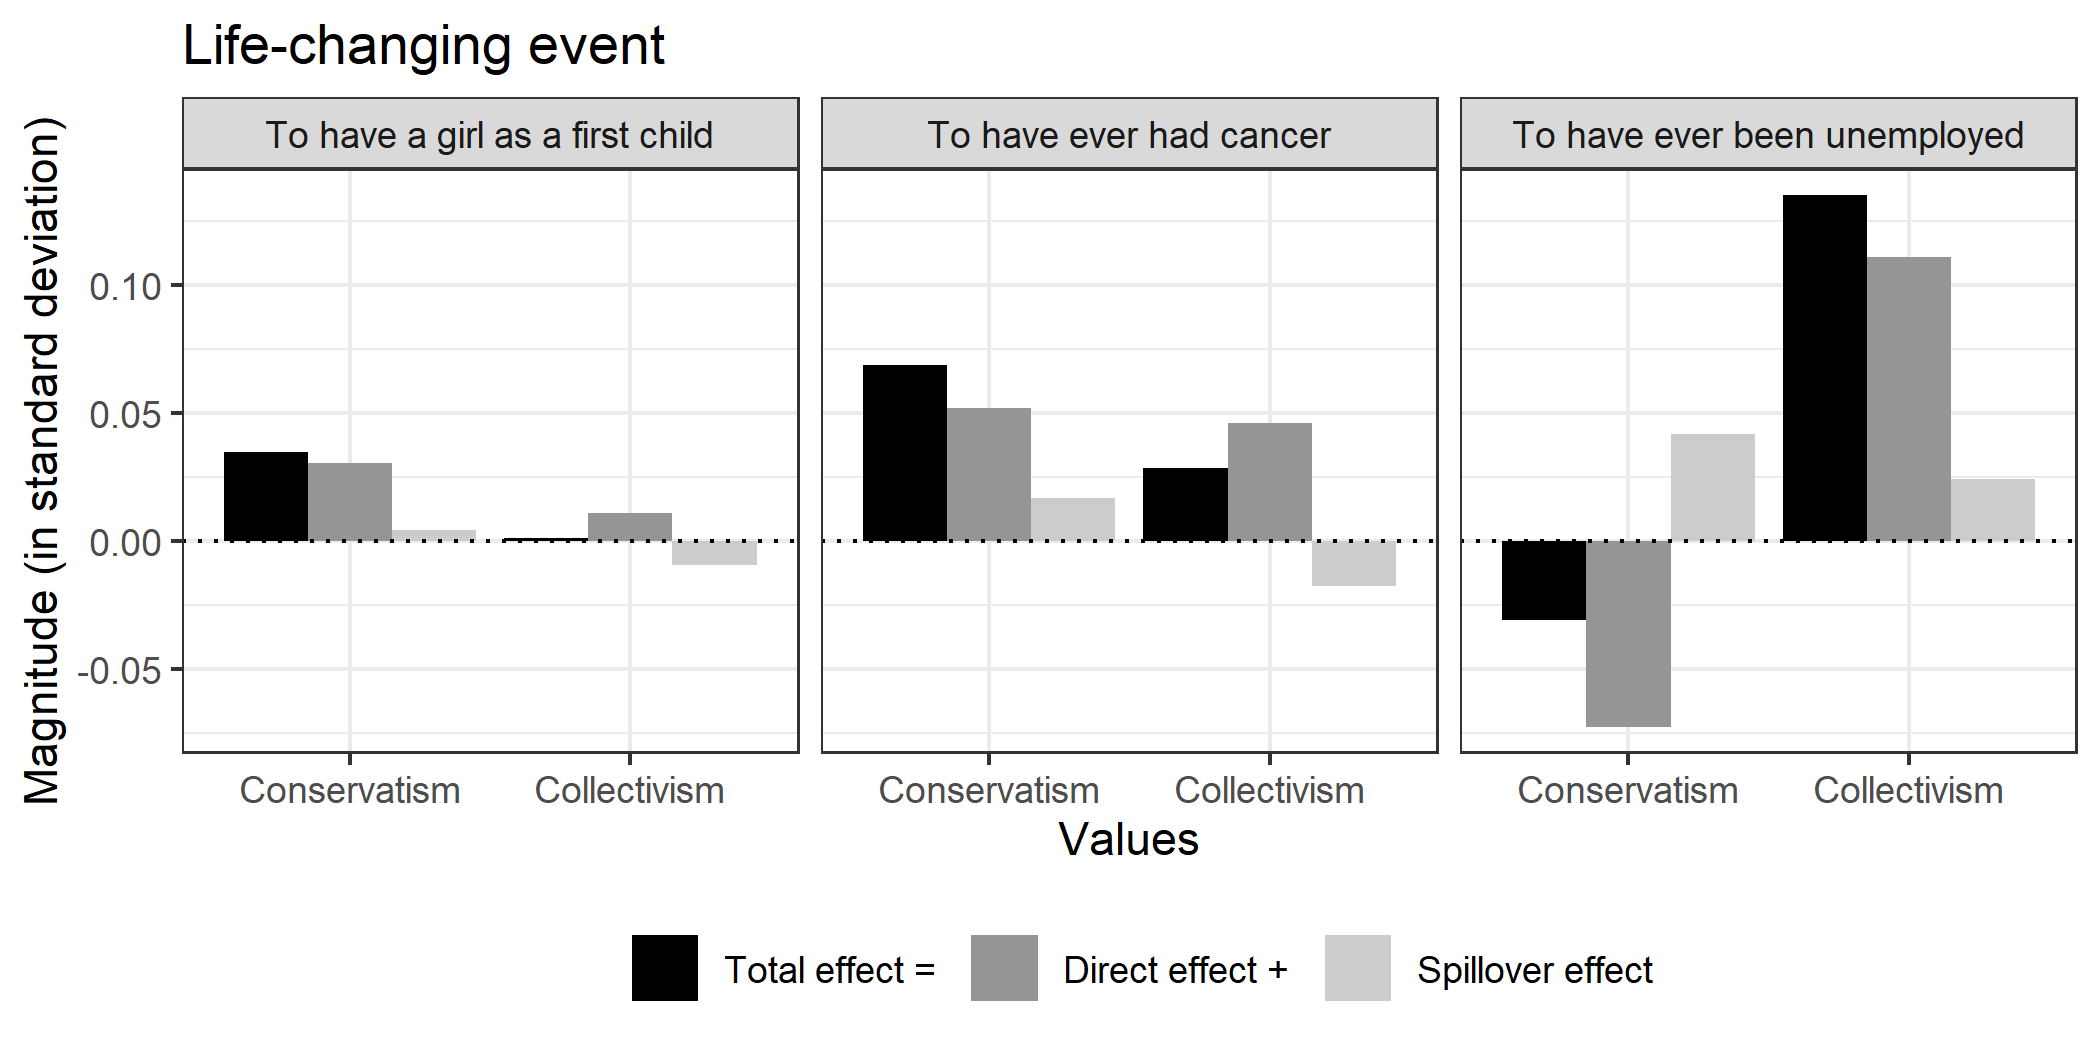
\includegraphics[width=\linewidth]{chap3/graphic/decomp-v5-base.png}
    \hrulefill
	\vspace{-3em}
	\justify\singlespacing\footnotesize{\textit{Notes:} This figure presents the decomposition of the total effect of each life-changing event on both values, Conservatism and Collectivism. The magnitude of effects is expressed in standard deviation. Decompositions are respectively derived from tables \ref{chap3-tab:decomp-GF}, \ref{chap3-tab:decomp-GC} and \ref{chap3-tab:decomp-BU}.}
\end{figure}
Having a girl as a first child directly increases conservative values by 0.03 standard deviation and collectivism by 0.01 standard deviation. Due to the consistency of values, about 14\% of the increase in conservatism is amplified by the raise in collectivism that has a positive impact on conservatism. Meanwhile, the increase in conservatism totally offsets the increase in collectivism, leading to a total effect that is negative although close to zero. Thus, due to the consistency of values and therefore the offsetting effect, collectivism does not increase when an individual gets a girl as a first child rather than a boy, while conservative values do increase. % This reconcile what we have seen in raw reg

Looking at heterogeneity across parents that are affected by this life event delivers two results (see figure \ref{chap3-fig:sem-decomp-v5-GFGender} and \ref{chap3-fig:sem-decomp-v5-GFEduc} in appendix \ref{chap3-estimates}). 
% Split by parents gender
First, for both, mothers and fathers, the direct effects go in the same direction---conservatism and collectivism---but they are more pronounced for mothers. For fathers, the negative spillover effect on collectivism offsets the positive information shock which leads to an increase in individualism. 
% Split by parents education
Second, splitting parents according to their education level shows that those with secondary education are the most affected. The effect of having a girl as a first child on tertiary-educated parents generates more progressive values which is consistent with \citet{Washington2008Female} results showing that congresspersons, hence, mostly highly educated men, become more progressive in their voting after having a daughter.

% HAVING EVER HAD CANCER
Having ever had cancer directly increases both conservatism and collectivism by 0.05 standard deviation. Due to values consistency, the increase in collectivism also increases conservative values through the spillover effect by 0.02 standard deviation, which represents almost a fourth of the total effect on conservatism. Meanwhile, part of the effect on collectivism is offset by the spillover effect of the life event through conservatism. As conservatism raises, it also decreases collectivism by 0.02 standard deviation which corresponds to 38\% of the direct effect. Thus, without the consistency of values, the increase in collectivism would have been 38\% much larger.

One may be concerned by the NCDS58 cohort at age 50 as they are likely to anticipate sickness, thus, changing their values. Excluding the NCDS58 cohort at age 50 provides very similar results with respect to the full sample, whereas considering exclusively this cohort at that age shows that the direct effect on conservatism is four times larger with respect to the baseline specification (see figure \ref{chap3-fig:sem-decomp-v5-GCNCDS58} in appendix \ref{chap3-estimates}). Interestingly, the direct effect on collectivism is much closer to zero. Thus, those who have had cancer at age 50 are not different from those who have not had one. Such an effect may be due to the anticipation of the sickness of the whole cohort at that age as they will rely more on others, hence, they increase their collectivist values. Nonetheless, the total effect on collectivism is positive---about 0.1 standard deviation---which is mostly due to the positive spillover effect on collectivism.
I also provide these estimates by focusing only on individuals who have never had cancer in the previous period (see figure \ref{chap3-fig:sem-decomp-v5-GCNever} in appendix \ref{chap3-estimates}). Although the direct effect on collectivism is larger, qualitative results hold.

% HAVING EVER BEEN UNEMPLOYED
Focusing on the third panel, those who have ever been unemployed experience a direct decline in conservatism, i.e. an increase in progressivism, by 0.07 standard deviation and a direct increase in collectivism by 0.11 standard deviation. The spillover effect of the decline in conservatism increases collectivist values by 0.02 standard deviation. Thus, collectivism raises by 22\% due to the spillover effect. Meanwhile, the increase in collectivism generates a positive spillover effect on conservative values which offsets half of the direct raise in progressivism. As a result, the increase in conservatism is dampened by the spillover effect whereas collectivism increases substantively.\footnote{In the extension of the theoretical framework in appendix \ref{chap3-model2}, I show that there is a bias when measuring the effect of an endogenous life event---such as unemployment---on values and I derive its expression. The bias does not affect the relative shares of the total effect that are due to the direct and spillover effects, nor the sign of the latter. However, the bias may affect the magnitude of the effect. In an extreme case of endogeneity of unemployment to values, the magnitudes have to be multiplied by a factor of 2/5, whereas feasible scenarii are likely to lie with a scale factor ranging from 1 (no endogeneity) to 2/3.}

One may be concerned by the current employment status that would be the driving factor for the effect of having ever been unemployed on values. I estimate the SEM using two subsamples (see figure \ref{chap3-fig:sem-decomp-v5-BUActivity} in appendix \ref{chap3-estimates}). First, I remove unemployed individuals at the time of the interview, then, I remove those out-of-work (unemployed and inactive). Both estimates do not differ with respect to the full sample one.

\subsection{Spillover effects' dynamics}

The intensity of inter-dependence between values drives the magnitude of the spillover effects of life events on values. In the SEM, the matrix $\Gamma$ captures the relation between values within the structural form. Once we consider the estimated reduced form for the decomposition, the spillover effects appear through $\Gamma^{-1}$. For instance, in the case of the girl-first life event, the $\Gamma$ matrix corresponds to
\begin{equation*}
    \Gamma = \begin{pmatrix}1 & 0.39 \\ -0.31 & 1\end{pmatrix} \implies \Gamma^{-1} = \begin{pmatrix}0.89 & -0.35 \\ 0.28 & 0.89\end{pmatrix}.
\end{equation*}
For both other life events, the coefficients in the matrices $\Gamma$ are very close to these ones which indicates that spillover effects do not depend on life events but are rather inherent.%
\footnote{See tables \ref{chap3-tab:reg-v5-sem-GC-stage12} and \ref{chap3-tab:reg-v5-sem-BU-stage12} in the appendix from which the $\Gamma$ matrix can be derived. For the got-cancer life event, $\Gamma = \begin{pmatrix}1 & 0.37 \\ -0.34 & 1\end{pmatrix}$. For the been-unmployed life event, $\Gamma = \begin{pmatrix}1 & 0.37 \\ -0.33 & 1\end{pmatrix}$.}
Thus, the effect of the life event $Z$ on values is derived from the matrix product of $\Theta = \begin{pmatrix} \theta_{Cons} & \theta_{Coll} \end{pmatrix}$ and the propagation matrix $\Gamma^{-1}$ that accounts for direct and spillover effects.

Considering the effect of the life event $Z$ on both values as a homogeneous system of first-order linear differential equations leads to
\begin{align*}
    x^\prime &= 0.89 x + 0.28 y,\\
    y^\prime &= -0.35 x + 0.89 y,
\end{align*}
where $x$ and $y$ are the magnitudes of both information shocks from $\Theta$, whereas $x^\prime$ and $y^\prime$ correspond to the net effects on values from $\Phi$. Solving this system leads to complex eigenvalues with positive real parts. This is due to the fact that, in $\Gamma$, the coefficients on the diagonal are equal to one and both off-diagonal coefficients have opposite signs. 

Figure \ref{chap3-fig:phase-plane} illustrates the phase plane of this system.
\begin{figure}[!tb]
    \centering
    \caption{Dynamics between values}
    \label{chap3-fig:phase-plane}
    \includegraphics[width=\linewidth]{chap3/graphic/sys-diff-eq-plus.png}
	\vspace{-3em}
	\justify\singlespacing\footnotesize{\textit{Notes:} This figure presents the phase plane of the homogeneous system of first-order linear differential equations that describes the relationship between conservatism (versus progressivism) and collectivism (versus individualism) values. Green arrows decompose the direct effect and the indirect effect, i.e. spillover effect, due to a one standard deviation increase in each value.}
\end{figure}
Green dots are set to 1 on both axis, thus, the green arrows describe what happens for a one standard deviation increase on either the x-axis or the y-axis, i.e. in conservatism or in collectivism. An increase in conservatism has a negative spillover effect on collectivism, while an increase in collectivism has a positive spillover effect on conservatism. Thus, the relationship between values is \textit{not reciprocal} because of the spiral pattern in the system of first-order linear differential equations that is derived from the propagation matrix $\Gamma$.

Social psychology literature provides dynamic principles that shed light on the spiral pattern. Those principles correspond to the dynamic underpinnings of changes in values and correspond to the four corners of the figure (see \citealt{Schwartz2012Overview} for more details). For instance, any simultaneous increase in both conservatism and collectivism values, hence toward the top-right corner, refers to a raise in \textit{social focus}, i.e. preferring to live within a community and reinforcing the stability, tradition, and conformity to that community. Conversely, a decrease in those two values, hence toward the bottom-left corner, correspond to a raise in \textit{personal focus}, i.e. preferring to focus on self and not being constrained by rules. Looking at the two other corners, when individualism increases along with conservatism, hence toward the bottom-right corner, this refers to changes in values that help to deal with anxiety and the fear of loss goals, thus, they are self-protective values. Conversely, the top-left corner corresponds to self-expansive and anxiety-free based values.

Examining the spiral pattern of spillover effects through the lens of the dynamic underpinnings of value changes from social psychology provides several keys to understanding how life events affect individuals' values in figure \ref{chap3-fig:sem-decomp-v5-base}.
First, the initial increase in conservatism for both girl-first and got-cancer life events generates a spillover in individualism as those two life events are associated with anxiety, hence, self-protective values. Meanwhile, the initial raise of collectivist values reinforces the increase in conservatism by generating a positive spillover as it triggers a rise in social focus, i.e. relying more on the community and its rules.
For the been-unemployed life event, the initial increase in progressivism characterizes an increase in anxiety-free values as the fear of unemployed is not relevant anymore compared to those who have never been unemployed, hence, preventing themselves from losses. This raise in anxiety-free values has a positive impact on collectivism. The direct effect on collectivism is positive as the individual had relied more on the community since she had been unemployed, thus, this increases the social focus, hence conservative values.
    
    \section{Summary and concluding remarks} \label{chap3-conclusion}
    An extensive literature has studied the effect of life experiences on values but supposing that values are independent. I present a framework that jointly analyzes the dynamics of values over the lifecycle when life events provide information shocks on values in a context where values are inter-dependent in society. My results suggest that values inter-dependence plays an important role as individuals seek to be consistent with respect to values held in the group with which they identify. Thus, neglecting this mechanism underestimates to which extent life experiences affect individuals.

This paper has two main limitations which relate to the theoretical framework. First, I assume that value frontiers between groups are exogenous, while they are most likely endogenous. In my theoretical framework, I assume that the population is sufficiently large to ensure the anonymity of the agent, meaning that any change of value from the agent does not change the distribution. Relaxing this hypothesis would make the value frontier between groups endogenous. It would also relate the theoretical framework to the literature on network. Considering, for instance, that some individuals are more influential than others according to their position within the network. Such a framework could lead to a new approach in linking behaviors, values, and networks in a context of inter-dependence between values. Although I do not consider this approach in this paper, I intend to explore it in future works.

Second, I focus on individual life events, hence, the model is a partial equilibrium model. Thus, I suppose that values held in the group are time-invariant. An extension of the model would be to make them time-dependent, hence, sufficiently large shocks in one period, such as economic crises or global pandemics, would affect the average values. However, this extension goes beyond the scope of the paper and is also intentionally left for future research.

This paper raises an issue that has not been considered in the economic literature yet, namely, the consequences of life events on values. As values are at the roots of agents' preferences---which themselves can explain gaps in economic outcomes---, I believe that values dynamics could be incorporated in future work to explain how observed gaps between individuals can be due to differences in exposure to life events. 
    
    \printbibliography[heading=subbibintoc]
    
    \clearpage
    \addsec{Appendices}
    \renewcommand{\thesubsection}{\thechapter.\Alph{subsection}}
    
    \subsection{Model details} \label{chap3-model}
    This appendix presents the details of the theoretical framework.

\begin{proof}[Proof of Proposition \ref{chap3-prp:converge}]
    The value converges as $\lim_{t\to+\infty} a_t = a^\star$ since $(\eta_a,\phi_a)\in(\mathbb{R}^\star_{+})^2$. The rate of convergence $\eta_a/(\eta_a+\phi_a)$ is a decreasing in $\phi_a/\eta_a$. The smaller the rate of convergence, the faster the speed of convergence. Therefore, the speed of convergence is an increasing function of the relative weight of the group consistency with respect to the time consistency in the utility function.
\end{proof}

\begin{proof}[Proof of Proposition \ref{chap3-prp:shock}]
$\forall s_t\in\{\underline{s}, \overline{s}\}, \forall a_t\in\mathbb{R},~\exists \Delta{a_t} > \Delta\widetilde{a}_t$ such that $\lim_{t\to+\infty} a_{t+1} = a^\star(-s_t)$
\end{proof}

\begin{proof}[Proof of Proposition \ref{chap3-prp:relevant}]
Starting with the expression of the indifference value $\widetilde{a}$ from equation, it is straightforward to show that $\frac{\partial^2\widetilde{a}}{\partial(\overline{b}-\underline{b})^2}>0$. In this example, $\widetilde{a}$ is a convex function of $\overline{b}-\underline{b}$. Thus, the greater the gap between both groups in value $b$ with respect to value $a$, the greater the information shock in value $a$ has to be so that the agent identifies to the other group. Therefore, the less relevant is this latter value in its choice of group membership.
\end{proof}

\begin{proof}[Proof of Proposition \ref{chap3-prp:spillover}]
If $\overline{b}-\underline{b}\neq 0$, then $\exists \Delta{a_t}$ such that $a_{t-1}^\prime > \widetilde{a}_{t-1}$ which implies that the individual identifies to the other group in period $t$. Therefore, both values $a_t$ and $b_t$ change.
\end{proof}

\textbf{Theoretical framework with three groups.}
One may ask to which extent the results hold with more than two groups. So, suppose that instead of having two groups in the reference population, we introduce a third group between both groups. I refer to the former groups as $s_A$ and $s_C$ instead of $\overline{s}$ and $\underline{s}$, while $s_B$ is the new group.

Starting with the single-value model, the ranking is as follows $a_A < a_B < a_C$. Reproducing figure \ref{chap3-fig:theory-choice-a} but with three groups leads to figure \ref{chap3-fig:theory-choice3-a}.
\begin{figure}[!ht]
    \centering
    \caption{Indifference value and group membership (with three groups)}
    \label{chap3-fig:theory-choice3-a}
    \includegraphics[width=.8\linewidth]{chap3/graphic/theory-choice3-a.png}
	\vspace{-3em}
	\justify\singlespacing\footnotesize{\textit{Notes:} This figure is an extension of figure \ref{chap3-fig:theory-choice-a} when there are three groups instead of two in the single value model. The figure presents the indifference values $\widetilde{a}_{ij}$ which are defined as the threshold values $a$ in $t-1$ such that the agent is indifferent between two groups. When the value $a$ in previous period lie in the area of one group, the agent prefers to identify to this group.}
\end{figure}
Introducing an additional group does not change the indifference value between two groups---which remains the midpoint value.
Propositions \ref{chap3-prp:converge} and \ref{chap3-prp:shock} hold in the three-group model.

Consider the two-value model by introducing the second value $b$. Assume the following ranking $a_C < a_B < a_A$ and $b_C < b_B < b_A$, which means that values are positively correlated across groups. I use the simplest case as an example, but other types of ranking are possible. Suppose the setup of section \ref{chap3-theoretical} with respect to the agent. She belongs to the group with the lowest value $a$, hence, $s_A$. It is still possible to derive the expression of the indifference value between the groups $A$ and $j\in\{B,C\}$ from equation \eqref{chap3-eq:indiff}, namely,
\begin{equation}\label{chap3-eq:indiff2}
    \widetilde{a}_{Aj} = \widehat{a}_{Aj} + \frac{1}{2\gamma}\frac{\big(b_j-b_A\big)^2}{a_j-a_A},
\end{equation}
where $\widehat{a}_{Aj}$ is the midpoint value between those of both groups $A$ and $j$. Since $a_j-a_A > 0$, it means that the second term of \eqref{chap3-eq:indiff2} is positive. As a result, the indifference value $\widetilde{a}$ is greater than the midpoint value. Both frontiers are pushed further right with respect to the single-value model in figure \ref{chap3-fig:theory-choice3-a}.

Under those conditions, it is still always possible to find an information shock such that the agent changes her group. Therefore, both propositions \ref{chap3-prp:relevant} and \ref{chap3-prp:spillover} hold. Although spillover effects still exist, their magnitudes are different with respect to the case with the two groups. Information shocks that move $a^\prime_{t-1}$ between $\widetilde{a}_{AB}$ and $\widetilde{a}_{BC}$ generate smaller spillover effects---with respect to the two-group model---as the agent identifies to the group $s_B$; while shocks that move $a^\prime_{t-1}$ beyond $\widetilde{a}_{BC}$ generate larger spillover effects.
    \clearpage
    \subsection{Statement details} \label{chap3-statement}
    This appendix presents the details of statements according to attitudes. These details have been split into three tables, namely, tables \ref{chap3-tab:statement-split-1}, \ref{chap3-tab:statement-split-2} and \ref{chap3-tab:statement-split-3}.

\begin{table}[!hb]
    \centering
    \caption{Statements details by attitudes - Part 1/3}
    \label{chap3-tab:statement-split-1}
    \resizebox*{\textwidth}{!}{
        \begin{threeparttable}
            \begin{tabular}{lll}
\toprule
Variable & Question & Rev\\
\midrule
\addlinespace[0.3em]
\multicolumn{3}{l}{\textbf{Authority (A)}}\\
\hline
\hspace{1em}A1 & The law should be obeyed, even if a particular law is wrong? & \\
\hspace{1em}A2 & For some crimes the death penalty is the most appropriate sentence? & \\
\hspace{1em}A3 & Censorship of films and magazines is necessary to uphold moral standards? & \\
\hspace{1em}A4 & People who break the law should be given stiffer sentences? & \\
\hspace{1em}A5 & Young people today don't have enough respect for traditional British values? & \\
\hspace{1em}A6 & Schools should teach children to obey authority? & \\
\addlinespace[0.3em]
\multicolumn{3}{l}{\textbf{Anti-Racism (AR)}}\\
\hline
\hspace{1em}AR1 & It is alright for people from different races to get married? & \\
\hspace{1em}AR2 & I would not mind if a family from another race moved in next door to me? & \\
\hspace{1em}AR3 & I would not mind if my child went to a school where half the children were of another race? & \\
\hspace{1em}AR4 & I would not mind working with people from other races? & \\
\hspace{1em}AR5 & I would not want a person from another race to be my boss? & X\\
\addlinespace[0.3em]
\multicolumn{3}{l}{\textbf{Children (C)}}\\
\hline
\hspace{1em}C1 & Unless you have children you'll be lonely when you get old? & \\
\hspace{1em}C2 & People can have a fulfilling life without having children? & X\\
\hspace{1em}C3 & Having children seriously interferes with the freedom of their parents? & X\\
\hspace{1em}C4 & People who never have children are missing an important part of life? & \\
\addlinespace[0.3em]
\multicolumn{3}{l}{\textbf{Environment (E)}}\\
\hline
\hspace{1em}E1 & Problems in the environment are not as serious as people claim? & X\\
\hspace{1em}E2 & We should tackle problems in the environment even if this means slower economic growth? & \\
\hspace{1em}E3 & Preserving the environment is more important than any other political issue today? & \\
\bottomrule
\end{tabular}

            \begin{tablenotes}[flushleft]
            \footnotesize{\item \textit{Notes}: The \textit{Rev} column indicates whether the scale has been reversed in the analysis.}
            \end{tablenotes}
        \end{threeparttable}
    }
\end{table}

\begin{table}[!htb]
    \centering
    \caption{Statements details by attitudes - Part 2/3}
    \label{chap3-tab:statement-split-2}
    \resizebox*{\textwidth}{!}{
        \begin{threeparttable}
            
\begin{tabular}{lll}
\toprule
Variable & Question & Rev\\
\midrule
\addlinespace[0.3em]
\multicolumn{3}{l}{\textbf{Inequality Aversion (IA)}}\\
\hline
\hspace{1em}IA1 & Big business benefits owners at the expense of the workers? & \\
\hspace{1em}IA2 & Private schools should be abolished? & \\
\hspace{1em}IA3 & Management will always try to get the better of employees if it gets the chance? & \\
\hspace{1em}IA4 & The time has come for everyone to arrange their own private health care and stop relying on the NHS? & X\\
\hspace{1em}IA5 & Ordinary working people do not get their fair share of the nation's wealth? & \\
\hspace{1em}IA6 & Government should redistribute income from the better off to those who are less well off? & \\
\hspace{1em}IA7 & There is one law for the rich and one for the poor? & \\
\addlinespace[0.3em]
\multicolumn{3}{l}{\textbf{Information Technology (IT)}}\\
\hline
\hspace{1em}IT1 & Computers at work are destroying people's skills? & X\\
\hspace{1em}IT2 & Computers enrich the lives of those who use them? & \\
\hspace{1em}IT3 & Every family should have a computer? & \\
\hspace{1em}IT4 & Learning to use a computer is more trouble than it's worth? & X\\
\addlinespace[0.3em]
\multicolumn{3}{l}{\textbf{Learning (L)}}\\
\hline
\hspace{1em}L1 & You are more likely to get a better job if you do some learning, training or education? & \\
\hspace{1em}L2 & For getting jobs, knowing the right people is more important than the qualifications? & X\\
\hspace{1em}L3 & Learning about new things boosts your confidence? & \\
\hspace{1em}L4 & The effort of getting qualifications is more trouble than it's worth? & X\\
\addlinespace[0.3em]
\multicolumn{3}{l}{\textbf{Morale (MOR)}}\\
\hline
\hspace{1em}MOR1 & Divorce is too easy to get these days? & \\
\hspace{1em}MOR2 & Married people are generally happier than unmarried people? & \\
\hspace{1em}MOR3 & Couples who have children should not separate? & \\
\hspace{1em}MOR4 & Marriage is for life? & \\
\hspace{1em}MOR5 & All women should have the right to choose an abortion if they wish? & X\\
\hspace{1em}MOR6 & It is alright for people to have children without being married? & X\\
\bottomrule
\end{tabular}

            \begin{tablenotes}[flushleft]
            \footnotesize{\item \textit{Notes}: The \textit{Rev} column indicates whether the scale has been reversed in the analysis.}
            \end{tablenotes}
        \end{threeparttable}}
\end{table}

\begin{table}[!htb]
    \centering
    \caption{Statements details by attitudes - Part 3/3}
    \label{chap3-tab:statement-split-3}
    \resizebox*{\textwidth}{!}{
        \begin{threeparttable}
            
\begin{tabular}{lll}
\toprule
Variable & Question & Rev\\
\midrule
\addlinespace[0.3em]
\multicolumn{3}{l}{\textbf{Political Cynicism (PC)}}\\
\hline
\hspace{1em}PC1 & None of the political parties would do anything to benefit me? & \\
\hspace{1em}PC2 & It does not really make much difference which political party is in power in Britain? & \\
\hspace{1em}PC3 & Politicians are mainly in politics for their own benefit and not for the benefit of the community? & \\
\addlinespace[0.3em]
\multicolumn{3}{l}{\textbf{Work-Ethic (WE)}}\\
\hline
\hspace{1em}WE1 & Having almost any job is better than being unemployed? & \\
\hspace{1em}WE2 & If I didn't like a job I'd pack it in, even if there was no other job to go to? & X\\
\hspace{1em}WE3 & Once you've got a job it's important to hang on to it even if you don't really like it? & \\
\addlinespace[0.3em]
\multicolumn{3}{l}{\textbf{Working Mother (WM)}}\\
\hline
\hspace{1em}WM1 & A pre-school child is likely to suffer if his or her mother works? & X\\
\hspace{1em}WM2 & All in all, family life suffers when the mother has a full time job? & X\\
\hspace{1em}WM3 & Children benefit if their mother has a job outside the home? & \\
\hspace{1em}WM4 & A mother and her family will all be happier if she goes out to work? & \\
\hspace{1em}WM5 & A father's job is to earn money; a mother's job is to look after the home and family? & X\\
\bottomrule
\end{tabular}

            \begin{tablenotes}[flushleft]
            \footnotesize{\item \textit{Notes}: The \textit{Rev} column indicates whether the scale has been reversed in the analysis.}
            \end{tablenotes}
        \end{threeparttable}}
\end{table}

    \clearpage
    \subsection{Principal component analysis} \label{chap3-pca}
    This appendix presents the principal components eigenvectors from the Principal Component Analysis (PCA) in section \ref{chap3-data}. Table \ref{chap3-tab:pca-v5-BCS70} presents the eigenvectors for the BCS70 cohort, while table \ref{chap3-tab:pca-v5-NCDS58} displays those for the NCDS58 cohort.

\begin{table}[!hb]
    \centering
    \caption{Principal components eigenvectors for the BCS70 cohort}
    \label{chap3-tab:pca-v5-BCS70}
    \begin{threeparttable}
        
\begin{tabular}{lrrrrr}
\toprule
  & \multicolumn{1}{c}{PC1} & \multicolumn{1}{c}{PC2} & \multicolumn{1}{c}{PC3} & \multicolumn{1}{c}{PC4} & \multicolumn{1}{c}{PC5}\\
\midrule
\addlinespace[0.3em]
\multicolumn{6}{l}{\textbf{Age 26}}\\
\hline
\hspace{1em}Authority & 0.622 & 0.011 & 0.136 & -0.146 & -0.757\\
\hspace{1em}Inequality Aversion & -0.182 & 0.686 & -0.533 & 0.348 & -0.303\\
\hspace{1em}Morale & 0.521 & 0.244 & -0.453 & -0.513 & 0.449\\
\hspace{1em}Political Cynicism & 0.149 & 0.656 & 0.695 & 0.065 & 0.245\\
\hspace{1em}Work Ethic & 0.535 & -0.200 & -0.093 & 0.769 & 0.272\\
\midrule
\hspace{1em}Standard deviation & 1.262 & 1.087 & 0.929 & 0.866 & 0.783\\
\hspace{1em}Proportion of Variance & 0.319 & 0.236 & 0.173 & 0.150 & 0.123\\
\hspace{1em}Cumulative Proportion & 0.319 & 0.555 & 0.727 & 0.877 & 1.000\\
\addlinespace[0.3em]
\multicolumn{6}{l}{\textbf{Age 30}}\\
\hline
\hspace{1em}Authority & 0.614 & -0.162 & -0.050 & 0.281 & -0.718\\
\hspace{1em}Inequality Aversion & 0.153 & 0.702 & 0.013 & -0.638 & -0.278\\
\hspace{1em}Morale & 0.534 & -0.109 & -0.678 & -0.202 & 0.450\\
\hspace{1em}Political Cynicism & 0.326 & 0.605 & 0.221 & 0.592 & 0.359\\
\hspace{1em}Work Ethic & 0.456 & -0.321 & 0.699 & -0.351 & 0.276\\
\midrule
\hspace{1em}Standard deviation & 1.243 & 1.137 & 0.918 & 0.827 & 0.797\\
\hspace{1em}Proportion of Variance & 0.309 & 0.259 & 0.169 & 0.137 & 0.127\\
\hspace{1em}Cumulative Proportion & 0.309 & 0.568 & 0.736 & 0.873 & 1.000\\
\addlinespace[0.3em]
\multicolumn{6}{l}{\textbf{Age 42}}\\
\hline
\hspace{1em}Authority & 0.570 & -0.360 & -0.004 & -0.519 & -0.526\\
\hspace{1em}Inequality Aversion & 0.172 & 0.722 & 0.172 & 0.280 & -0.584\\
\hspace{1em}Morale & 0.462 & -0.048 & -0.749 & 0.466 & 0.079\\
\hspace{1em}Political Cynicism & 0.517 & 0.474 & 0.122 & -0.368 & 0.598\\
\hspace{1em}Work Ethic & 0.406 & -0.350 & 0.628 & 0.548 & 0.135\\
\midrule
\hspace{1em}Standard deviation & 1.184 & 1.124 & 0.968 & 0.882 & 0.787\\
\hspace{1em}Proportion of Variance & 0.281 & 0.253 & 0.187 & 0.156 & 0.124\\
\hspace{1em}Cumulative Proportion & 0.281 & 0.533 & 0.721 & 0.876 & 1.000\\
\bottomrule
\end{tabular}

        % \begin{tablenotes}[flushleft]
        %     \footnotesize{\item \textit{Notes}: Signs of the eigenvectors have been inverted for age 30 and age 42 in order to have the same axis direction for the first principal component. The attitude toward Inequality Aversion (IA) is removed for the PCA on the BCS70 cohort at the age of 26 years because only one statement is available.}
        % \end{tablenotes}
    \end{threeparttable}
\end{table}

\begin{table}[!htb]
    \centering
    \caption{Principal components eigenvectors for the NCDS58 cohort}
    \label{chap3-tab:pca-v5-NCDS58}
    \begin{threeparttable}
        
\begin{tabular}{lrrrrr}
\toprule
  & \multicolumn{1}{c}{PC1} & \multicolumn{1}{c}{PC2} & \multicolumn{1}{c}{PC3} & \multicolumn{1}{c}{PC4} & \multicolumn{1}{c}{PC5}\\
\midrule
\addlinespace[0.3em]
\multicolumn{6}{l}{\textbf{Age 33}}\\
\hline
\hspace{1em}Authority & 0.607 & -0.150 & 0.155 & -0.546 & 0.535\\
\hspace{1em}Inequality Aversion & 0.006 & 0.730 & -0.072 & 0.353 & 0.580\\
\hspace{1em}Morale & 0.548 & -0.077 & 0.551 & 0.591 & -0.201\\
\hspace{1em}Political Cynicism & 0.276 & 0.654 & 0.053 & -0.414 & -0.567\\
\hspace{1em}Work Ethic & 0.504 & -0.102 & -0.815 & 0.237 & -0.122\\
\midrule
\hspace{1em}Standard deviation & 1.250 & 1.162 & 0.901 & 0.851 & 0.741\\
\hspace{1em}Proportion of Variance & 0.313 & 0.270 & 0.162 & 0.145 & 0.110\\
\hspace{1em}Cumulative Proportion & 0.313 & 0.583 & 0.745 & 0.890 & 1.000\\
\addlinespace[0.3em]
\multicolumn{6}{l}{\textbf{Age 42}}\\
\hline
\hspace{1em}Authority & 0.605 & -0.141 & -0.156 & 0.369 & 0.674\\
\hspace{1em}Inequality Aversion & 0.173 & 0.713 & 0.178 & -0.559 & 0.342\\
\hspace{1em}Morale & 0.500 & -0.245 & -0.542 & -0.534 & -0.333\\
\hspace{1em}Political Cynicism & 0.446 & 0.521 & 0.038 & 0.480 & -0.546\\
\hspace{1em}Work Ethic & 0.395 & -0.375 & 0.805 & -0.187 & -0.144\\
\midrule
\hspace{1em}Standard deviation & 1.258 & 1.101 & 0.916 & 0.875 & 0.775\\
\hspace{1em}Proportion of Variance & 0.317 & 0.242 & 0.168 & 0.153 & 0.120\\
\hspace{1em}Cumulative Proportion & 0.317 & 0.559 & 0.727 & 0.880 & 1.000\\
\addlinespace[0.3em]
\multicolumn{6}{l}{\textbf{Age 50}}\\
\hline
\hspace{1em}Authority & 0.531 & -0.134 & 0.063 & -0.816 & -0.173\\
\hspace{1em}Inequality Aversion & 0.554 & 0.296 & -0.075 & 0.441 & -0.637\\
\hspace{1em}Morale & 0.157 & -0.663 & -0.716 & 0.152 & 0.018\\
\hspace{1em}Political Cynicism & 0.578 & 0.264 & -0.063 & 0.170 & 0.750\\
\hspace{1em}Work Ethic & 0.229 & -0.620 & 0.689 & 0.296 & 0.033\\
\midrule
\hspace{1em}Standard deviation & 1.373 & 1.046 & 0.945 & 0.804 & 0.694\\
\hspace{1em}Proportion of Variance & 0.377 & 0.219 & 0.179 & 0.129 & 0.096\\
\hspace{1em}Cumulative Proportion & 0.377 & 0.596 & 0.775 & 0.904 & 1.000\\
\bottomrule
\end{tabular}

        % \begin{tablenotes}[flushleft]
        %     \footnotesize{\item \textit{Notes}: Signs of eigenvectors have been inverted for age 33 and age 50 in order to have the same axis direction for the first principal component.}
        % \end{tablenotes}
    \end{threeparttable}
\end{table}

\begin{figure}[!htb]
    \caption{Two-dimensional structure of universal motivational types of values}
    \label{chap3-fig:schwartz}
    \centering
    \includegraphics[width=.8\linewidth]{chap3/graphic/schwartz92.png}
	\vspace{-3em}
	\justify\singlespacing\footnotesize{\textit{Notes:} This figure reproduces the two-dimensional structure of motivational types of values from \citet{Schwartz1992Universals, Schwartz2012Overview}.}
\end{figure}
    \clearpage
    \subsection{Data details} \label{chap3-details}
    This appendix presents the details of the data. Table \ref{chap3-tab:data-vote} shows the shares of vote in general elections in both cohorts.

\begin{table}[!htb]
    \centering
    \caption{Shares of vote in general elections in both cohorts}
    \label{chap3-tab:data-vote}
    \begin{threeparttable}
        % \setlength{\tabcolsep}{5pt}
        
\begin{tabular}{llrrrrrr}
\toprule
\multicolumn{1}{c}{} & \multicolumn{1}{c}{} & \multicolumn{6}{c}{Proportion of total (in percent)} \\
\cmidrule(l{3pt}r{3pt}){3-8}
  &   & Other & Con & Grn & Lab & LD & UKIP\\
\midrule
BCS70 & Age 26 (GE 1997) & 45.5 & 15.6 & 0.5 & 30.8 & 7.6 & \\
BCS70 & Age 30 (GE 2001) & 51.6 & 13.0 & 1.0 & 25.8 & 7.8 & 0.8\\
BCS70 & Age 42 (GE 2010) & 30.4 & 28.8 & 1.7 & 23.1 & 14.3 & 1.7\\
\midrule
NCDS58 & Age 33 (GE 1987) & 27.6 & 34.0 &  & 26.8 & 11.6 & \\
NCDS58 & Age 42 (GE 1997) & 27.6 & 21.5 & 0.6 & 40.5 & 9.8 & \\
NCDS58 & Age 50 (GE 2010) & 43.2 & 22.9 & 1.1 & 19.0 & 10.8 & 3.0\\
\bottomrule
\end{tabular}

        \begin{tablenotes}[flushleft]
            \footnotesize{\item \textit{Notes}: This table presents the vote proportions (in percentage) for both cohorts at different ages according to the closest General Election (GE). Political parties are (in alphabetical order): Conservative (Con), Green (Grn), Labour (Lab), Liberal Democrat (LD), and UK Independence Party (UKIP). Other encompasses all other parties, blank votes and abstention.}
        \end{tablenotes}
    \end{threeparttable}
\end{table}
    \clearpage
    \subsection{Estimates} \label{chap3-estimates}
    This appendix presents additional regression tables of the paper. 
% RAW ESTIMATE
Table \ref{chap3-tab:reg-v5-raw-all-long} presents the long-version table of the regression table \ref{chap3-tab:reg-v5-raw-all-short} in the paper.
% INSTRUMENTAL VARIABLE
Table \ref{chap3-tab:reg-v5-IV-GFGC-long} presents the IV estimate of the spillover effects. Tables \ref{chap3-tab:reg-v5-IV-GFvote} and \ref{chap3-tab:reg-v5-IV-GCvote} correspond to the IV estimate of the group membership.
% SEM
Table \ref{chap3-tab:reg-v5-sem-GF-stage12}, \ref{chap3-tab:reg-v5-sem-GC-stage12}, and \ref{chap3-tab:reg-v5-sem-BU-stage12} present the details of the 2SLS estimates of the SEM for, respectively, the girl-first, got-cancer, and been-unemployed life event.
% DECOMPOSITION
Tables \ref{chap3-tab:decomp-GF}, \ref{chap3-tab:decomp-GC}, and \ref{chap3-tab:decomp-BU} summarize the decomposition of the total effect from the SEM for, respectively, the girl-first, got-cancer, and been-unemployed life event.
% ROBUSTNESS
Figure \ref{chap3-fig:sem-decomp-v5-GFGender} summarizes the decomposition of the total
effect of girl-first life event by parent. 
Figure \ref{chap3-fig:sem-decomp-v5-GFEduc} summarizes the decomposition of the total
effect of girl-first life event by education level.
Figure \ref{chap3-fig:sem-decomp-v5-BUActivity} summarizes the decomposition of the total
effect of been-unemployed life event according to the current activity status.

%%%%% APPLIED %%%%%

\begin{table}[!htb]
    \centering
    \caption{Effect of life events on values}
    \label{chap3-tab:reg-v5-raw-all-long}
    % \resizebox*{\textwidth}{!}{
    \begin{threeparttable}
        \setlength{\tabcolsep}{0pt}
        \begin{tabular}{l D{.}{.}{5.5} D{.}{.}{5.5} D{.}{.}{5.5} D{.}{.}{5.5} D{.}{.}{5.5} D{.}{.}{5.5}}
\toprule
 & \multicolumn{6}{c}{Linear regression - OLS} \\
\cmidrule(lr){2-7}
 & \multicolumn{2}{c}{GirlFirst} & \multicolumn{2}{c}{GotCancer} & \multicolumn{2}{c}{BeenUnemp} \\
\cmidrule(lr){2-3}\cmidrule(lr){4-5}\cmidrule(lr){6-7}
 & \multicolumn{1}{c}{(Cons)} & \multicolumn{1}{c}{(Coll)} & \multicolumn{1}{c}{(Cons)} & \multicolumn{1}{c}{(Coll)} & \multicolumn{1}{c}{(Cons)} & \multicolumn{1}{c}{(Coll)} \\
\midrule
Intercept       & 0.32^{***}  & -0.15^{***} & 0.27^{***}  & -0.07^{***} & 0.26^{***}  & -0.11^{***} \\
                & (0.02)      & (0.02)      & (0.01)      & (0.01)      & (0.01)      & (0.01)      \\
Female          & -0.19^{***} & 0.07^{***}  & -0.17^{***} & 0.02        & -0.17^{***} & 0.03^{***}  \\
                & (0.01)      & (0.01)      & (0.01)      & (0.01)      & (0.01)      & (0.01)      \\
Educ. Secondary & -0.29^{***} & -0.04^{**}  & -0.28^{***} & -0.03^{**}  & -0.28^{***} & -0.03^{**}  \\
                & (0.02)      & (0.02)      & (0.01)      & (0.01)      & (0.01)      & (0.01)      \\
Educ. Tertiary  & -0.52^{***} & -0.04^{**}  & -0.50^{***} & -0.03^{**}  & -0.50^{***} & -0.03^{***} \\
                & (0.02)      & (0.02)      & (0.01)      & (0.01)      & (0.01)      & (0.01)      \\
Life event      & 0.03^{**}   & 0.00        & 0.09^{***}  & 0.02        & 0.02^{*}    & 0.18^{***}  \\
                & (0.01)      & (0.01)      & (0.03)      & (0.03)      & (0.01)      & (0.01)      \\
Value$_{t-1}$   & 0.54^{***}  & 0.49^{***}  & 0.56^{***}  & 0.50^{***}  & 0.56^{***}  & 0.49^{***}  \\
                & (0.01)      & (0.01)      & (0.00)      & (0.00)      & (0.00)      & (0.00)      \\
\midrule
R$^2$ & \multicolumn{1}{c}{0.37} & \multicolumn{1}{c}{0.26} & \multicolumn{1}{c}{0.39} & \multicolumn{1}{c}{0.27} & \multicolumn{1}{c}{0.39} & \multicolumn{1}{c}{0.27}\\
Adj. R$^2$ & \multicolumn{1}{c}{0.37} & \multicolumn{1}{c}{0.26} & \multicolumn{1}{c}{0.39} & \multicolumn{1}{c}{0.27} & \multicolumn{1}{c}{0.39} & \multicolumn{1}{c}{0.27}\\
Num. obs. & \multicolumn{1}{c}{23354} & \multicolumn{1}{c}{23354} & \multicolumn{1}{c}{32885} & \multicolumn{1}{c}{32885} & \multicolumn{1}{c}{32885} & \multicolumn{1}{c}{32885}\\
\bottomrule
\end{tabular}

        \begin{tablenotes}[flushleft]
            \footnotesize{\item \textit{Notes}: $^{***}p<0.01$; $^{**}p<0.05$; $^{*}p<0.1$. Standard errors between parentheses. Male in the NCDS cohort in his forties with primary education as the reference group. GirlFirst and GotCancer are the life events. In GirlFirst regressions, parents who have had a boy as a first child are the reference group. In GotCancer regressions, individuals who never had a cancer are the reference group. In BeenUnemp, individuals who have never been unemployed are the reference group. Table \ref{chap3-tab:reg-v5-raw-all-short} in the paper summarizes the coefficients.}
        \end{tablenotes}
    \end{threeparttable}
    % }
\end{table}

\begin{table}[!htb]
    \centering
    \caption{IV Estimate of the spillover effect}
    \label{chap3-tab:reg-v5-IV-GFGC-long}
    \begin{threeparttable}
        \begin{tabular}{l D{.}{.}{5.5} D{.}{.}{5.5} D{.}{.}{5.5} D{.}{.}{5.5}}
\toprule
 & \multicolumn{4}{c}{IV regression - 2SLS} \\
\cmidrule(lr){2-5}
 & \multicolumn{2}{c}{GirlFirst} & \multicolumn{2}{c}{GotCancer} \\
\cmidrule(lr){2-3}\cmidrule(lr){4-5}
 & \multicolumn{1}{c}{(Cons)} & \multicolumn{1}{c}{(Coll)} & \multicolumn{1}{c}{(Cons)} & \multicolumn{1}{c}{(Coll)} \\
\midrule
Intercept                 & 0.32^{***}  & 0.07^{***}  & 0.27^{***}  & 0.10^{***}  \\
                          & (0.02)      & (0.02)      & (0.01)      & (0.01)      \\
Female                    & -0.19^{***} & -0.02^{**}  & -0.17^{***} & -0.06^{***} \\
                          & (0.01)      & (0.01)      & (0.01)      & (0.01)      \\
Educ. Secondary           & -0.29^{***} & -0.18^{***} & -0.28^{***} & -0.19^{***} \\
                          & (0.02)      & (0.02)      & (0.01)      & (0.01)      \\
Educ. Tertiary            & -0.52^{***} & -0.33^{***} & -0.50^{***} & -0.36^{***} \\
                          & (0.02)      & (0.02)      & (0.01)      & (0.01)      \\
Life event                & 0.03^{**}   &             & 0.09^{***}  &             \\
                          & (0.01)      &             & (0.03)      &             \\
$\widehat{\text{Cons}}_t$ &             & -0.32^{***} &             & -0.34^{***} \\
                          &             & (0.01)      &             & (0.01)      \\
Value$_{t-1}$             & 0.54^{***}  & 0.48^{***}  & 0.56^{***}  & 0.49^{***}  \\
                          & (0.01)      & (0.01)      & (0.00)      & (0.00)      \\
\midrule
R$^2$ & \multicolumn{1}{c}{0.37} & \multicolumn{1}{c}{0.30} & \multicolumn{1}{c}{0.39} & \multicolumn{1}{c}{0.31}\\
Adj. R$^2$ & \multicolumn{1}{c}{0.37} & \multicolumn{1}{c}{0.30} & \multicolumn{1}{c}{0.39} & \multicolumn{1}{c}{0.31}\\
Num. obs. & \multicolumn{1}{c}{23354} & \multicolumn{1}{c}{23354} & \multicolumn{1}{c}{32885} & \multicolumn{1}{c}{32885}\\
\bottomrule
\end{tabular}

        \begin{tablenotes}[flushleft]
            \footnotesize{\item \textit{Notes}: $^{***}p<0.01$; $^{**}p<0.05$; $^{*}p<0.1$. Standard errors between parentheses. Control variables include gender, education (primary, secondary, tertiary), cohort fixed effects and period fixed effects. Male in the NCDS cohort in his forties with primary education as the reference group. GirlFirst and GotCancer are the life events. In GirlFirst regressions, parents who have had a boy as a first child are the reference group. In GotCancer regressions, individuals who never had a cancer are the reference group. Table \ref{chap3-tab:reg-v5-IV-GFGC-short} in the paper summarizes the coefficients.}
        \end{tablenotes}
    \end{threeparttable}
    % }
\end{table}

\begin{table}[!htb]
    \centering
    \caption{IV Estimate of the group membership (GirlFirst)}
    \label{chap3-tab:reg-v5-IV-GFvote}
    \begin{threeparttable}
        \setlength{\tabcolsep}{3pt}
        \begin{tabular}{l D{.}{.}{5.5} D{.}{.}{5.5} D{.}{.}{5.5} D{.}{.}{5.5} D{.}{.}{5.5}}
\toprule
 & \multicolumn{5}{c}{IV regression - GirlFirst - Multinomial logit - Dep. var.: Vote} \\
\cmidrule(lr){2-6}
 & \multicolumn{1}{c}{(Con)} & \multicolumn{1}{c}{(Grn)} & \multicolumn{1}{c}{(Lab)} & \multicolumn{1}{c}{(LD)} & \multicolumn{1}{c}{(UKIP)} \\
\midrule
Intercept                 & -1.41^{***} & -3.58^{***} & -1.10^{***} & -1.98^{***} & -5.08      \\
                          & (0.04)      & (0.14)      & (0.04)      & (0.05)      & (3.22)     \\
Female                    & -0.15^{***} & 0.04        & -0.04       & -0.02       & -0.27^{**} \\
                          & (0.04)      & (0.15)      & (0.04)      & (0.05)      & (0.12)     \\
Educ. Secondary           & 0.56^{***}  & 0.35^{*}    & 0.09^{*}    & 0.55^{***}  & 0.08       \\
                          & (0.05)      & (0.20)      & (0.05)      & (0.07)      & (0.16)     \\
Educ. Tertiary            & 0.78^{***}  & 0.62^{***}  & 0.36^{***}  & 0.94^{***}  & -0.22      \\
                          & (0.06)      & (0.19)      & (0.06)      & (0.07)      & (0.20)     \\
$\widehat{\text{Cons}}_t$ & 0.01        & -0.85^{***} & -0.27^{***} & -0.34^{***} & 0.18^{*}   \\
                          & (0.03)      & (0.10)      & (0.03)      & (0.04)      & (0.09)     \\
Con $\text{Vote}_{t-1}$   & 2.56^{***}  & 0.13        & 0.46^{***}  & 0.91^{***}  & 1.27^{***} \\
                          & (0.05)      & (0.27)      & (0.06)      & (0.08)      & (0.18)     \\
Grn $\text{Vote}_{t-1}$   & 0.63^{*}    & 3.75^{***}  & 0.77^{**}   & 1.59^{***}  & 0.49       \\
                          & (0.33)      & (0.31)      & (0.35)      & (0.31)      & (1.03)     \\
Lab $\text{Vote}_{t-1}$   & 0.50^{***}  & 0.81^{***}  & 2.19^{***}  & 1.01^{***}  & 1.14^{***} \\
                          & (0.06)      & (0.18)      & (0.05)      & (0.07)      & (0.15)     \\
LD $\text{Vote}_{t-1}$    & 1.06^{***}  & 1.02^{***}  & 1.08^{***}  & 2.73^{***}  & 1.71^{***} \\
                          & (0.08)      & (0.25)      & (0.08)      & (0.08)      & (0.20)     \\
UKIP $\text{Vote}_{t-1}$  & 1.57^{***}  & 1.46        & -0.02       & 1.21^{**}   & 3.25^{***} \\
                          & (0.38)      & (1.06)      & (0.66)      & (0.50)      & (0.49)     \\
\midrule
Num. obs. & \multicolumn{1}{c}{23354} & \multicolumn{1}{c}{23354} & \multicolumn{1}{c}{23354} & \multicolumn{1}{c}{23354} & \multicolumn{1}{c}{23354}\\
\bottomrule
\end{tabular}

        \begin{tablenotes}[flushleft]
            \footnotesize{\item \textit{Notes}: $^{***}p<0.01$; $^{**}p<0.05$; $^{*}p<0.1$. Standard errors between parentheses. Control variables include gender, education (primary, secondary, tertiary), cohort fixed effects and period fixed effects. Male in the NCDS cohort in his forties with primary education as the reference group. GirlFirst and GotCancer are the life events. Parents who have had a boy as a first child are the reference group.
            % Multinomial
            The baseline outcome of the multinomial logistic regression is the vote for Other (encompassing all other parties, blank votes and abstention). $\text{Vote}_{t-1}$ corresponds to the effect of having voted for the corresponding party in the previous period.
            Table \ref{chap3-tab:reg-v5-IV-GFGCvote-short} in the paper summarizes the coefficients.}
        \end{tablenotes}
    \end{threeparttable}
    % }
\end{table}

\begin{table}[!htb]
    \centering
    \caption{IV Estimate of the group membership (GotCancer)}
    \label{chap3-tab:reg-v5-IV-GCvote}
    \begin{threeparttable}
        \setlength{\tabcolsep}{3pt}
        \begin{tabular}{l D{.}{.}{5.5} D{.}{.}{5.5} D{.}{.}{5.5} D{.}{.}{5.5} D{.}{.}{5.5}}
\toprule
 & \multicolumn{5}{c}{IV regression - GotCancer - Multinomial logit - Dep. var.: Vote} \\
\cmidrule(lr){2-6}
 & \multicolumn{1}{c}{(Con)} & \multicolumn{1}{c}{(Grn)} & \multicolumn{1}{c}{(Lab)} & \multicolumn{1}{c}{(LD)} & \multicolumn{1}{c}{(UKIP)} \\
\midrule
Intercept                 & -1.43^{***} & -3.47^{***} & -1.19^{***} & -1.97^{***} & -5.49       \\
                          & (0.03)      & (0.10)      & (0.03)      & (0.04)      & (11.53)     \\
Female                    & -0.09^{***} & 0.08        & 0.03        & 0.06        & -0.28^{***} \\
                          & (0.03)      & (0.11)      & (0.03)      & (0.04)      & (0.10)      \\
Educ. Secondary           & 0.58^{***}  & 0.23        & 0.09^{**}   & 0.50^{***}  & 0.06        \\
                          & (0.04)      & (0.16)      & (0.04)      & (0.06)      & (0.13)      \\
Educ. Tertiary            & 0.74^{***}  & 0.65^{***}  & 0.36^{***}  & 0.88^{***}  & -0.22       \\
                          & (0.05)      & (0.14)      & (0.04)      & (0.06)      & (0.16)      \\
$\widehat{\text{Cons}}_t$ & 0.08^{***}  & -0.67^{***} & -0.24^{***} & -0.32^{***} & 0.19^{**}   \\
                          & (0.03)      & (0.07)      & (0.02)      & (0.03)      & (0.07)      \\
Con $\text{Vote}_{t-1}$   & 2.56^{***}  & 0.09        & 0.47^{***}  & 0.82^{***}  & 1.22^{***}  \\
                          & (0.04)      & (0.21)      & (0.05)      & (0.07)      & (0.15)      \\
Grn $\text{Vote}_{t-1}$   & 0.29        & 3.31^{***}  & 0.36        & 1.24^{***}  & 1.28^{***}  \\
                          & (0.25)      & (0.23)      & (0.27)      & (0.23)      & (0.48)      \\
Lab $\text{Vote}_{t-1}$   & 0.41^{***}  & 0.73^{***}  & 2.21^{***}  & 0.99^{***}  & 0.87^{***}  \\
                          & (0.05)      & (0.14)      & (0.04)      & (0.06)      & (0.13)      \\
LD $\text{Vote}_{t-1}$    & 1.00^{***}  & 1.17^{***}  & 1.11^{***}  & 2.71^{***}  & 1.54^{***}  \\
                          & (0.07)      & (0.18)      & (0.06)      & (0.06)      & (0.16)      \\
UKIP $\text{Vote}_{t-1}$  & 1.46^{***}  & 1.60^{**}   & -0.03       & 1.28^{***}  & 3.06^{***}  \\
                          & (0.32)      & (0.77)      & (0.57)      & (0.41)      & (0.42)      \\
\midrule
Num. obs. & \multicolumn{1}{c}{32885} & \multicolumn{1}{c}{32885} & \multicolumn{1}{c}{32885} & \multicolumn{1}{c}{32885} & \multicolumn{1}{c}{32885}\\
\bottomrule
\end{tabular}

        \begin{tablenotes}[flushleft]
            \footnotesize{\item \textit{Notes}: $^{***}p<0.01$; $^{**}p<0.05$; $^{*}p<0.1$. Standard errors between parentheses. Control variables include gender, education (primary, secondary, tertiary), cohort fixed effects and period fixed effects. Male in the NCDS cohort in his forties with primary education as the reference group. GirlFirst and GotCancer are the life events. Individuals who never had a cancer are the reference group.
            % Multinomial
            The baseline outcome of the multinomial logistic regression is the vote for Other (encompassing all other parties, blank votes and abstention). $\text{Vote}_{t-1}$ corresponds to the effect of having voted for the corresponding party in the previous period.
            Table \ref{chap3-tab:reg-v5-IV-GFGCvote-short} in the paper summarizes the coefficients.}
        \end{tablenotes}
    \end{threeparttable}
    % }
\end{table}

\begin{table}[!htb]
    \centering
    \caption{SEM Estimate of the spillover effects (GirlFirst)}
    \label{chap3-tab:reg-v5-sem-GF-stage12}
    % \resizebox*{\textwidth}{!}{
    \begin{threeparttable}
        \begin{tabular}{l D{.}{.}{5.5} D{.}{.}{5.5} D{.}{.}{5.5} D{.}{.}{5.5}}
\toprule
 & \multicolumn{4}{c}{2SLS regression} \\
\cmidrule(lr){2-5}
 & \multicolumn{2}{c}{Reduced form (Stage 1)} & \multicolumn{2}{c}{Structural form (Stage 2)} \\
\cmidrule(lr){2-3}\cmidrule(lr){4-5}
 & \multicolumn{1}{c}{(Cons)} & \multicolumn{1}{c}{(Coll)} & \multicolumn{1}{c}{(Cons)} & \multicolumn{1}{c}{(Coll)} \\
\midrule
GirlFirst                 & 0.03^{***} & 0.00        & 0.03^{***} & 0.01        \\
                          & (0.01)     & (0.01)      & (0.01)     & (0.01)      \\
Cons$_{t-1}$              & 0.55^{***} & -0.17^{***} & 0.62^{***} &             \\
                          & (0.01)     & (0.01)      & (0.01)     &             \\
Coll$_{t-1}$              & 0.19^{***} & 0.48^{***}  &            & 0.54^{***}  \\
                          & (0.01)     & (0.01)      &            & (0.01)      \\
$\widehat{\text{Cons}}_t$ &            &             &            & -0.31^{***} \\
                          &            &             &            & (0.01)      \\
$\widehat{\text{Coll}}_t$ &            &             & 0.39^{***} &             \\
                          &            &             & (0.01)     &             \\
\midrule
R$^2$ & \multicolumn{1}{c}{0.40} & \multicolumn{1}{c}{0.30} & \multicolumn{1}{c}{0.40} & \multicolumn{1}{c}{0.30}\\
Adj. R$^2$ & \multicolumn{1}{c}{0.40} & \multicolumn{1}{c}{0.30} & \multicolumn{1}{c}{0.40} & \multicolumn{1}{c}{0.30}\\
Num. obs. & \multicolumn{1}{c}{23354} & \multicolumn{1}{c}{23354} & \multicolumn{1}{c}{23354} & \multicolumn{1}{c}{23354}\\
\bottomrule
\end{tabular}

        \begin{tablenotes}[flushleft]
            \footnotesize{\item \textit{Notes}: $^{***}p<0.01$; $^{**}p<0.05$; $^{*}p<0.1$. Standard errors between parentheses. Control variables in all regressions include cohort, period, gender and education.}
        \end{tablenotes}
    \end{threeparttable}%}
\end{table}

\begin{table}[!htb]
    \centering
    \caption{SEM Estimate of the spillover effects (GotCancer)}
    \label{chap3-tab:reg-v5-sem-GC-stage12}
    % \resizebox*{\textwidth}{!}{
    \begin{threeparttable}
        \begin{tabular}{l D{.}{.}{5.5} D{.}{.}{5.5} D{.}{.}{5.5} D{.}{.}{5.5}}
\toprule
 & \multicolumn{4}{c}{2SLS regression} \\
\cmidrule(lr){2-5}
 & \multicolumn{2}{c}{Reduced form (Stage 1)} & \multicolumn{2}{c}{Structural form (Stage 2)} \\
\cmidrule(lr){2-3}\cmidrule(lr){4-5}
 & \multicolumn{1}{c}{(Cons)} & \multicolumn{1}{c}{(Coll)} & \multicolumn{1}{c}{(Cons)} & \multicolumn{1}{c}{(Coll)} \\
\midrule
GotCancer                 & 0.07^{**}  & 0.03        & 0.06^{*}   & 0.05^{*}    \\
                          & (0.03)     & (0.03)      & (0.03)     & (0.03)      \\
Cons$_{t-1}$              & 0.57^{***} & -0.19^{***} & 0.64^{***} &             \\
                          & (0.00)     & (0.00)      & (0.00)     &             \\
Coll$_{t-1}$              & 0.18^{***} & 0.49^{***}  &            & 0.55^{***}  \\
                          & (0.00)     & (0.00)      &            & (0.00)      \\
$\widehat{\text{Cons}}_t$ &            &             &            & -0.34^{***} \\
                          &            &             &            & (0.01)      \\
$\widehat{\text{Coll}}_t$ &            &             & 0.37^{***} &             \\
                          &            &             & (0.01)     &             \\
\midrule
R$^2$ & \multicolumn{1}{c}{0.42} & \multicolumn{1}{c}{0.31} & \multicolumn{1}{c}{0.42} & \multicolumn{1}{c}{0.31}\\
Adj. R$^2$ & \multicolumn{1}{c}{0.42} & \multicolumn{1}{c}{0.31} & \multicolumn{1}{c}{0.42} & \multicolumn{1}{c}{0.31}\\
Num. obs. & \multicolumn{1}{c}{32885} & \multicolumn{1}{c}{32885} & \multicolumn{1}{c}{32885} & \multicolumn{1}{c}{32885}\\
\bottomrule
\end{tabular}

        \begin{tablenotes}[flushleft]
            \footnotesize{\item \textit{Notes}: $^{***}p<0.01$; $^{**}p<0.05$; $^{*}p<0.1$. Standard errors between parentheses. Control variables in all regressions include cohort, period, gender and education.}
        \end{tablenotes}
    \end{threeparttable}%}
\end{table}

\begin{table}[!htb]
    \centering
    \caption{SEM Estimate of the spillover effects (BeenUnemp)}
    \label{chap3-tab:reg-v5-sem-BU-stage12}
    % \resizebox*{\textwidth}{!}{
    \begin{threeparttable}
        \begin{tabular}{l D{.}{.}{5.5} D{.}{.}{5.5} D{.}{.}{5.5} D{.}{.}{5.5}}
\toprule
 & \multicolumn{4}{c}{2SLS regression} \\
\cmidrule(lr){2-5}
 & \multicolumn{2}{c}{Reduced form (Stage 1)} & \multicolumn{2}{c}{Structural form (Stage 2)} \\
\cmidrule(lr){2-3}\cmidrule(lr){4-5}
 & \multicolumn{1}{c}{(Cons)} & \multicolumn{1}{c}{(Coll)} & \multicolumn{1}{c}{(Cons)} & \multicolumn{1}{c}{(Coll)} \\
\midrule
BeenUnemp                 & -0.03^{***} & 0.14^{***}  & -0.08^{***} & 0.12^{***}  \\
                          & (0.01)      & (0.01)      & (0.01)      & (0.01)      \\
Cons$_{t-1}$              & 0.57^{***}  & -0.19^{***} & 0.64^{***}  &             \\
                          & (0.00)      & (0.00)      & (0.00)      &             \\
Coll$_{t-1}$              & 0.18^{***}  & 0.48^{***}  &             & 0.54^{***}  \\
                          & (0.00)      & (0.00)      &             & (0.00)      \\
$\widehat{\text{Cons}}_t$ &             &             &             & -0.33^{***} \\
                          &             &             &             & (0.01)      \\
$\widehat{\text{Coll}}_t$ &             &             & 0.37^{***}  &             \\
                          &             &             & (0.01)      &             \\
\midrule
R$^2$ & \multicolumn{1}{c}{0.42} & \multicolumn{1}{c}{0.31} & \multicolumn{1}{c}{0.42} & \multicolumn{1}{c}{0.31}\\
Adj. R$^2$ & \multicolumn{1}{c}{0.42} & \multicolumn{1}{c}{0.31} & \multicolumn{1}{c}{0.42} & \multicolumn{1}{c}{0.31}\\
Num. obs. & \multicolumn{1}{c}{32885} & \multicolumn{1}{c}{32885} & \multicolumn{1}{c}{32885} & \multicolumn{1}{c}{32885}\\
\bottomrule
\end{tabular}

        \begin{tablenotes}[flushleft]
            \footnotesize{\item \textit{Notes}: $^{***}p<0.01$; $^{**}p<0.05$; $^{*}p<0.1$. Standard errors between parentheses. Control variables in all regressions include cohort, period, gender and education.}
        \end{tablenotes}
    \end{threeparttable}%}
\end{table}

\begin{table}[!htb]
    \centering
    \caption{Decomposition of the effect of GirlFirst on values}
    \label{chap3-tab:decomp-GF}
    \begin{threeparttable}
        \setlength{\tabcolsep}{12pt}
        
\begin{tabular}{lrrr}
\toprule
\multicolumn{1}{c}{ } & \multicolumn{2}{c}{Direct and indirect effects} & \multicolumn{1}{c}{Total effect} \\
\cmidrule(l{3pt}r{3pt}){2-3} \cmidrule(l{3pt}r{3pt}){4-4}
\multicolumn{1}{c}{Value ($v$)} & \multicolumn{1}{c}{$\widetilde{\gamma}^{Cons}_v \times \theta_{Cons}$} & \multicolumn{1}{c}{$\widetilde{\gamma}^{Coll}_v \times \theta_{Coll}$} & \multicolumn{1}{c}{${\phi}_v$}\\
\midrule
Conservatism ($Cons$) & \textbf{0.030} & 0.004 & 0.035\\
 & \textbf{(100.0)} & (13.9) & (113.9)\\
Collectivism ($Coll$) & -0.010 & \textbf{0.011} & 0.001\\
 & (-88.2) & \textbf{(100.0)} & (11.8)\\
\bottomrule
\end{tabular}

        \begin{tablenotes}[flushleft]
            \footnotesize{\item \textit{Notes}: Magnitudes in standard deviations. Direct effects in bold. Relative share with respect to the direct effect in percent between parentheses.}
        \end{tablenotes}
    \end{threeparttable}
\end{table}

\begin{table}[!htb]
    \centering
    \caption{Decomposition of the effect of GotCancer on values}
    \label{chap3-tab:decomp-GC}
    \begin{threeparttable}
        \setlength{\tabcolsep}{12pt}
        
\begin{tabular}{lrrr}
\toprule
\multicolumn{1}{c}{ } & \multicolumn{2}{c}{Direct and indirect effects} & \multicolumn{1}{c}{Total effect} \\
\cmidrule(l{3pt}r{3pt}){2-3} \cmidrule(l{3pt}r{3pt}){4-4}
\multicolumn{1}{c}{Value ($v$)} & \multicolumn{1}{c}{$\widetilde{\gamma}^{Cons}_v \times \theta_{Cons}$} & \multicolumn{1}{c}{$\widetilde{\gamma}^{Coll}_v \times \theta_{Coll}$} & \multicolumn{1}{c}{${\phi}_v$}\\
\midrule
Conservatism ($Cons$) & \textbf{0.052} & 0.017 & 0.069\\
 & \textbf{(100.0)} & (32.5) & (132.5)\\
Collectivism ($Coll$) & -0.018 & \textbf{0.046} & 0.029\\
 & (-38.1) & \textbf{(100.0)} & (61.9)\\
\bottomrule
\end{tabular}

        \begin{tablenotes}[flushleft]
            \footnotesize{\item \textit{Notes}: Magnitudes in standard deviations. Direct effects in bold. Relative share with respect to the direct effect in percent between parentheses.}
        \end{tablenotes}
    \end{threeparttable}
\end{table}

\begin{table}[!htb]
    \centering
    \caption{Decomposition of the effect of BeenUnemp on values}
    \label{chap3-tab:decomp-BU}
    \begin{threeparttable}
        \setlength{\tabcolsep}{12pt}
        
\begin{tabular}{lrrr}
\toprule
\multicolumn{1}{c}{ } & \multicolumn{2}{c}{Direct and indirect effects} & \multicolumn{1}{c}{Total effect} \\
\cmidrule(l{3pt}r{3pt}){2-3} \cmidrule(l{3pt}r{3pt}){4-4}
\multicolumn{1}{c}{Value ($v$)} & \multicolumn{1}{c}{$\widetilde{\gamma}^{Cons}_v \times \theta_{Cons}$} & \multicolumn{1}{c}{$\widetilde{\gamma}^{Coll}_v \times \theta_{Coll}$} & \multicolumn{1}{c}{${\phi}_v$}\\
\midrule
Conservatism ($Cons$) & \textbf{-0.073} & 0.042 & -0.031\\
 & \textbf{(100.0)} & (-57.2) & (42.8)\\
Collectivism ($Coll$) & 0.024 & \textbf{0.111} & 0.135\\
 & (21.7) & \textbf{(100.0)} & (121.7)\\
\bottomrule
\end{tabular}

        \begin{tablenotes}[flushleft]
            \footnotesize{\item \textit{Notes}: Magnitudes in standard deviations. Direct effects in bold. Relative share with respect to the direct effect in percent between parentheses.}
        \end{tablenotes}
    \end{threeparttable}
\end{table}

\begin{figure}[!htb]
    \centering
    \caption{Decomposition of the effect of GirlFirst by parent}
    \label{chap3-fig:sem-decomp-v5-GFGender}
    \includegraphics[width=\linewidth]{chap3/graphic/decomp-v5-GFGender.png}
    \hrulefill
	\vspace{-3em}
	\justify\singlespacing\footnotesize{\textit{Notes:} This figure presents the decomposition of the total effect of the girl-first life event on both values, Conservation and Collectivism, according to the parent. The magnitude of each effect is expressed in standard deviation.}
\end{figure}

\begin{figure}[!htb]
    \centering
    \caption{Decomposition of the effect of GirlFirst by education}
    \label{chap3-fig:sem-decomp-v5-GFEduc}
    \includegraphics[width=\linewidth]{chap3/graphic/decomp-v5-GFEduc.png}
    \hrulefill
	\vspace{-3em}
	\justify\singlespacing\footnotesize{\textit{Notes:} This figure presents the decomposition of the total effect of the girl-first life event on both values, Conservation and Collectivism, according to education. The magnitude of each effect is expressed in standard deviation.}
\end{figure}

\begin{figure}[!htb]
    \centering
    \caption{Decomposition of the effect of GotCancer with and without the NCDS58 Age 50}
    \label{chap3-fig:sem-decomp-v5-GCNCDS58}
    \includegraphics[width=\linewidth]{chap3/graphic/decomp-v5-GCNCDS58.png}
    \hrulefill
	\vspace{-3em}
	\justify\singlespacing\footnotesize{\textit{Notes:} This figure presents the decomposition of the total effect of the got-cancer life event on both values, Conservation and Collectivism, for the NCDS58 cohort at age 50 only and without them. The magnitude of each effect is expressed in standard deviation.}
\end{figure}

\begin{figure}[!htb]
    \centering
    \caption{Decomposition of the effect of GotCancer for those who never have had cancer before}
    \label{chap3-fig:sem-decomp-v5-GCNever}
    \includegraphics[width=\linewidth]{chap3/graphic/decomp-v5-GCNever.png}
    \hrulefill
	\vspace{-3em}
	\justify\singlespacing\footnotesize{\textit{Notes:} This figure presents the decomposition of the total effect of the got-cancer life event on both values, Conservation and Collectivism, for the NCDS58 cohort at age 50 only and without them. The magnitude of each effect is expressed in standard deviation.}
\end{figure}

\begin{figure}[!htb]
    \centering
    \caption{Decomposition of the effect of BeenUnemp by current activity status}
    \label{chap3-fig:sem-decomp-v5-BUActivity}
    \includegraphics[width=\linewidth]{chap3/graphic/decomp-v5-BUActivity.png}
    \hrulefill
	\vspace{-3em}
	\justify\singlespacing\footnotesize{\textit{Notes:} This figure presents the decomposition of the total effect of the girl-first life event on both values, Conservation and Collectivism, according to the current activity status. The magnitude of each effect is expressed in standard deviation.}
\end{figure}
    \clearpage
    \subsection{Extension of the theoretical framework} \label{chap3-model2}
    To quantify the effect of life events on values, we compare two individuals based on their life trajectories and values. Suppose there exist two individuals $i$ and $j$ that are identical except in their initial value $a_0$, with $a_0^j > a_0^i$. Both individuals belong to the group $\underline{s}$.
Let $\pi_t = \pi(a_t)$ be the probability that a life event occurs which is endogenous to the value $a$.

Suppose the information shock $\Delta a_0$---due to the life event---has the same magnitude for both individuals and would be sufficiently large such that both individuals would identify to the other group. The expected values $a_1$ and $b_1$ for the individual $j$ are
\begin{align}
    \mathbb{E}(a_1^j) &= \frac{\eta_a a^j_0 + \phi_a \underline{a}}{\eta_a+\phi_a} + \pi(a_0^j)\left[ \frac{\eta_a\Delta a_0 + \phi_a(\overline{a}-\underline{a})}{\eta_a+\phi_a} \right],\\
    \mathbb{E}(b_1^j) &= \frac{\eta_b b^j_0 + \phi_b \underline{b}}{\eta_b+\phi_b} + \pi(a_0^j)\frac{\phi_b(\overline{b}-\underline{b})}{\eta_b+\phi_b},
\end{align}
where $\mathbb{E}$ is the expectation operator. It is straightforward to show that these values are symmetrical for the individual $i$. Hence, the biases due to the endogeneity of values can be written as 
\begin{align}
    \mathbb{E}(a_1^j) - a_1^j &= \pi(a_0^j)\times\Delta A,\\
    \mathbb{E}(b_1^j) - b_1^j&= \pi(a_0^j)\times\Delta B,
\end{align}
where $\Delta A \equiv \frac{\eta_a\Delta a_0 + \phi_a(\overline{a}-\underline{a})}{\eta_a+\phi_a}$ is the direct effect of the life changing event on value $a$, and $\Delta B \equiv  \frac{\phi_b(\overline{b}-\underline{b})}{\eta_b+\phi_b}$ is the spillover effect of the life event on value $b$.


Let $\Delta\mathbb{E}v_t$ be the difference in expected value $v_t$ with respect to the true difference between both individuals, namely,
\begin{equation}
    \Delta\mathbb{E}v_t \equiv \mathbb{E}(v_t^j) - \mathbb{E}(v_t^i) - (v_t^j - v_t^i)
\end{equation}
% Suppose both individuals have the same initial values $a_0$. Then, it is straightforward to show that $\Delta\mathbb{E}v_1 = 0$ which means they have the same expected value in period $1$. In our case,
Thus,
\begin{align}
    \Delta\mathbb{E}a_1 &= \left[\pi(a_0^j) - \pi(a_0^i)\right]\times\Delta A,\label{chap3-eq:DeltaA}\\
    \Delta\mathbb{E}b_1 &= \left[\pi(a_0^j) - \pi(a_0^i)\right]\times\Delta B,\label{chap3-eq:DeltaB}
\end{align}
When the probability that the life event occurs is exogenous to values, i.e. $\pi(a_0^j) = \pi(a_0^i)$, there is no bias when estimating the difference between both individuals. 
However, in many cases such as unemployment, this probability is likely to be endogenous, i.e. $\pi(a_0^j) \neq \pi(a_0^i)$, which leads to a bias when gauging the effect of a life event on values.

The magnitude of the bias depends on two components: the difference in terms of probabilities that captures the degree of endogeneity of the life event with respect to values; and the magnitude of either the direct effect or the spillover effect. 
Although the endogeneity issue affects the magnitude of the total effect, it does not change the relative shares of the direct and spillover effects because it is a scale factor of the total effect.

In order to evaluate the magnitude of the bias, I assume that the probability $\pi(a_t)$ is an increasing function of $a_t$. The individual $j$ is more likely to face the life event since $a_0^j > a_0^i$. For simplicity, let assume a binomial logistic function such that
\begin{equation}
    \pi(a_0, \beta_a) = \frac{e^{\beta_a a_0}}{1 + e^{\beta_a a_0}}.
\end{equation}
Note that the intercept has been omitted. Suppose a large endogeneity, namely, that the advantage in terms of the probability that the life event occurs given by a higher value $a$ has an odd-ratio about $2$, which means that an individual with a one-standard-deviation increase in $a_0$ would be two times more likely that the life event occurs. As $\beta_a$ corresponds to the log-odd ratio, it implies that $\beta_a = \log(2)$. 

Table \ref{chap3-tab:gap-a0} summarizes the size of the bias according to the gap in initial values between both individuals.
\begin{table}[!tb]
    \centering
    \caption{Endogeneity bias}
    \label{chap3-tab:gap-a0}
    \begin{threeparttable}
        \setlength{\tabcolsep}{9pt}{}
        \begin{tabular}{lrrrrrrr}
            \toprule 
            & \multicolumn{7}{c}{$\beta_a = \log(2)$} \\
            \cmidrule(lr){2-8}
            $a_0^j$ & -2 & -1 & -0.5 & 0 & 0.5 & 1 & 2\\
            $a_0^i$ & 2 & 1 & 0.5 & 0 & -0.5 & -1 & -2\\
            \midrule
            $\pi(a_0^j)$ & 0.2 & 0.33 & 0.41 & 0.5 & 0.59 & 0.66 & 0.8\\
            $\pi(a_0^i)$ & 0.8 & 0.66 & 0.59 & 0.5 & 0.41 & 0.33 & 0.2\\
            \midrule
            $\Delta\pi$ & -0.6 & -0.33 & -0.17 & 0 & 0.17 & 0.33 & 0.6\\
            \bottomrule
        \end{tabular}
        \begin{tablenotes}[flushleft]
            \footnotesize{\item \textit{Notes}: This table presents the magnitude of the endogeneity bias due to the difference in initial value $a$ between two individuals. $\pi(a_0, \beta_a)$ corresponds to the probability derived from the binomial logistic function and $\Delta\pi$ to the difference in probabilities between both individuals.}
        \end{tablenotes}
    \end{threeparttable}
\end{table}
Since $\lvert \Delta\pi \rvert < 1$, it implies that the endogeneity bias does not change the sign of the direct and indirect effects. 
The (2, -2) and (-2, 2) scenarii are extreme cases in which there is a high degree of polarization in terms of values such that both groups have respectively 2 and -2 standard deviations on average while the average value in the population remains 0. Even in those extreme cases, both the direct and spillover effects can be biased by at the most a scale factor of plus or minus $0.6$.

\end{refsection}

	\chapter*{General Conclusion}
	\addcontentsline{toc}{chapter}{General Conclusion}
    \markboth{General Conclusion}{General Conclusion}
	This thesis examines the role of inter-generational dynamics in driving distributional outcomes: chapter one describes how inter-generational conflicts over the public policy can drive labor share dynamics, chapter two explores the link between labor market polarization and social mobility, and chapter three shows the existence of spillover effects across values.
It uses a wide range of techniques by providing theoretical models to confront them to data using a broad spectrum of empirical techniques ranging from the estimation of simultaneous equations models to calibration. The key contribution lies in the conclusion that inter-generational dynamics drive distributional outcomes through several mechanisms such as conflicts, social inequality reproduction, and transmissions of values.

The two first chapters provide evidence of the link between inter-generational dynamics and the labor market. In chapter one, I argue that the inter-generational conflict over the public budget allocation has consequences for wage bargaining in the labor market and therefore for the labor share. This chapter suggests that---to understand macroeconomic dynamics in the long run---we should take into account changes in institutions that are endogenously determined by the age structure of the population. In this regard, my results provide a new conceptual framework to examine demographic dynamics and institutions in future work.

In chapter two, we show that parental income has become more important in explaining children's occupational outcomes when they enter the labor market, but also thereafter. Using British cohort data, we suggest that the structure of employment affects not only the distribution of earnings but also the degree of occupational mobility. There may be a transmission of polarization across generations, thus the increased importance of parental background may accumulate across generations creating a multiplier effect that over time that accentuates the occupational distance across groups from different backgrounds.

The second and third chapters show how intra-generational dynamics are key in understanding inter-generational ones. In chapter two, we provide a bridge between the literatures on inter- and intra-generational mobility by focusing on access to jobs at the beginning of the career and the subsequent career dynamics. Thus, we show that understanding intra-generational mobility is essential to understanding an individual’s outcome when mature. In chapter three, I argue that, within a cohort, as individuals go through different life experiences they change their values with respect to those of their peers. Those changes in values are either directly due to life events or indirectly due to spillover effects. Thus, I provide an intra-generational mechanism that is complementary to the inter-generational transmission of values.


% \printbibliography[heading=subbibliography]

\end{document}
